\documentclass[11pt]{report}
\usepackage[utf8]{inputenc}
\usepackage[margin=1in]{geometry}
\usepackage{amsmath, amssymb, amsthm}
\usepackage{mathtools}
\usepackage{enumitem}
\usepackage{hyperref}
\usepackage{xcolor}
\usepackage{tikz-cd}
\usetikzlibrary{calc,arrows.meta}
\usepackage{tcolorbox}
\usepackage{titlesec}

% Keep section numbering continuous across chapters
\makeatletter
\@removefromreset{section}{chapter}
\makeatother
\renewcommand{\thesection}{\S\arabic{section}}
\renewcommand{\thesubsection}{\arabic{section}.\arabic{subsection}}

% ============================================================================
% AXLER-STYLE COLOR SCHEME
% ============================================================================
% Blue for theorems/propositions/lemmas/corollaries (results to prove)
\definecolor{axlerblue}{RGB}{200, 220, 240}
\definecolor{axlerblueborder}{RGB}{100, 140, 180}

% Yellow/cream for definitions (things to memorize)
\definecolor{axleryellow}{RGB}{255, 250, 205}
\definecolor{axleryellowborder}{RGB}{200, 180, 100}

% Green for examples
\definecolor{axlergreen}{RGB}{220, 245, 220}
\definecolor{axlergreenborder}{RGB}{100, 160, 100}

% Gray for remarks/notes
\definecolor{axlergray}{RGB}{245, 245, 245}
\definecolor{axlergrayborder}{RGB}{180, 180, 180}

% Purple for motivation/intuition remarks
\definecolor{axlerpurple}{RGB}{235, 222, 245}
\definecolor{axlerpurpleborder}{RGB}{140, 100, 180}

% Orange for exercises/questions
\definecolor{axlerorange}{RGB}{255, 235, 205}
\definecolor{axlerorangeborder}{RGB}{200, 150, 100}

% ============================================================================
% AXLER-STYLE THEOREM BOXES
% ============================================================================
\tcbuselibrary{theorems, skins, breakable}

% Separate counters for each type
\newcounter{defcounter}[section]
\renewcommand{\thedefcounter}{\thesection.\arabic{defcounter}}

\newcounter{thmcounter}[section]
\renewcommand{\thethmcounter}{\thesection.\arabic{thmcounter}}

\newcounter{excounter}[section]
\renewcommand{\theexcounter}{\thesection.\arabic{excounter}}

% Definition box (yellow)
\newtcolorbox[use counter=defcounter]{defbox}[1][]{
    enhanced,
    colback=axleryellow,
    colframe=axleryellowborder,
    fonttitle=\bfseries,
    title=Definition \arabic{section}.\arabic{defcounter}\ifx\\#1\\\else: #1\fi,
    breakable,
    left=3mm, right=3mm, top=2mm, bottom=2mm,
    before skip=10pt, after skip=10pt
}

% Theorem box (blue)
\newtcolorbox[use counter=thmcounter]{thmbox}[1][]{
    enhanced,
    colback=axlerblue,
    colframe=axlerblueborder,
    fonttitle=\bfseries,
    title=Theorem \arabic{section}.\arabic{thmcounter}\ifx\\#1\\\else: #1\fi,
    breakable,
    left=3mm, right=3mm, top=2mm, bottom=2mm,
    before skip=10pt, after skip=10pt
}

% Lemma box (blue, lighter) - shares counter with theorem
\newtcolorbox[use counter=thmcounter]{lembox}[1][]{
    enhanced,
    colback=axlerblue!70,
    colframe=axlerblueborder,
    fonttitle=\bfseries,
    title=Lemma \arabic{section}.\arabic{thmcounter}\ifx\\#1\\\else: #1\fi,
    breakable,
    left=3mm, right=3mm, top=2mm, bottom=2mm,
    before skip=10pt, after skip=10pt
}

% Proposition box (blue) - shares counter with theorem
\newtcolorbox[use counter=thmcounter]{propbox}[1][]{
    enhanced,
    colback=axlerblue!80,
    colframe=axlerblueborder,
    fonttitle=\bfseries,
    title=Proposition \arabic{section}.\arabic{thmcounter}\ifx\\#1\\\else: #1\fi,
    breakable,
    left=3mm, right=3mm, top=2mm, bottom=2mm,
    before skip=10pt, after skip=10pt
}

% Corollary box (blue, lighter) - shares counter with theorem
\newtcolorbox[use counter=thmcounter]{corbox}[1][]{
    enhanced,
    colback=axlerblue!60,
    colframe=axlerblueborder,
    fonttitle=\bfseries,
    title=Corollary \arabic{section}.\arabic{thmcounter}\ifx\\#1\\\else: #1\fi,
    breakable,
    left=3mm, right=3mm, top=2mm, bottom=2mm,
    before skip=10pt, after skip=10pt
}

% Example box (green)
\newtcolorbox[use counter=excounter]{exbox}[1][]{
    enhanced,
    colback=axlergreen,
    colframe=axlergreenborder,
    fonttitle=\bfseries,
    title=Example \arabic{section}.\arabic{excounter}\ifx\\#1\\\else: #1\fi,
    breakable,
    left=3mm, right=3mm, top=2mm, bottom=2mm,
    before skip=10pt, after skip=10pt
}

% Remark box (purple)
\newtcolorbox{rembox}[1][]{
    enhanced,
    colback=axlerpurple,
    colframe=axlerpurpleborder,
    fonttitle=\bfseries,
    title=Remark\ifx\\#1\\\else: #1\fi,
    breakable,
    left=3mm, right=3mm, top=2mm, bottom=2mm,
    before skip=10pt, after skip=10pt
}

% Exercise/Question box (orange)
\newtcolorbox{questbox}[1][]{
    enhanced,
    colback=axlerorange,
    colframe=axlerorangeborder,
    fonttitle=\bfseries,
    title=Question\ifx\\#1\\\else: #1\fi,
    breakable,
    left=3mm, right=3mm, top=2mm, bottom=2mm,
    before skip=10pt, after skip=10pt
}

% Proof environment
\renewenvironment{proof}[1][Proof]{\noindent\textbf{#1.} }{\hfill$\square$\par\vspace{5pt}}

% ============================================================================
% DOCUMENT SETTINGS
% ============================================================================
\setlength{\parindent}{0pt}
\setlength{\parskip}{6pt}
\setcounter{tocdepth}{3}
\setcounter{secnumdepth}{3}


% ---- Cross-reference labels for the colored boxes (section.n numbering) ----
\makeatletter
\newcommand{\thmlabel}[1]{\edef\@currentlabel{\arabic{section}.\arabic{thmcounter}}\label{#1}}
\newcommand{\deflabel}[1]{\edef\@currentlabel{\arabic{section}.\arabic{defcounter}}\label{#1}}
\newcommand{\exlabel}[1]{\edef\@currentlabel{\arabic{section}.\arabic{excounter}}\label{#1}}
\makeatother

% ---- Matrix-group macros ----
\newcommand{\GL}{\mathrm{GL}}
\newcommand{\SL}{\mathrm{SL}}
\newcommand{\Ogp}{\mathrm{O}}
\newcommand{\SO}{\mathrm{SO}}
\newcommand{\Ugp}{\mathrm{U}}
\DeclareMathOperator{\Mat}{Mat}
\DeclareMathOperator{\tr}{tr}
\DeclareMathOperator{\adj}{adj}
\DeclareMathOperator{\sgn}{sgn}
\newcommand{\Gr}{\mathrm{Gr}}
\DeclareMathOperator{\Span}{span}
\DeclareMathOperator{\Sym}{Sym}
\DeclareMathOperator{\Skew}{Skew}
\DeclareMathOperator{\Herm}{Herm}
\newcommand{\geo}{\mathrm{geo}}
% Roadmap markers: thread / stage line at the head of each section
\newcommand{\roadmark}[2]{\par\noindent{\small\textsc{#1}\quad\textit{#2}}\par\medskip}
% Reference to the corresponding result in Lee, Introduction to Smooth Manifolds (2nd ed.)
\newcommand{\leeref}[1]{\par\smallskip{\raggedleft\footnotesize\textsc{Lee}:\ #1\par}}

\usetikzlibrary{decorations.markings}
\usepackage{longtable,booktabs,array}
\title{\textbf{MATH 591: Differentiable Manifolds} \\ \large Lecture Notes}
\author{Tianshuo Wang}
\date{Fall 2026}

\begin{document}
\maketitle

\begin{center}
\fbox{\parbox{0.85\textwidth}{
\textbf{Instructor:} A.\ Uribe. \quad \textbf{Text:} Lee, \emph{Introduction to Smooth Manifolds} (2nd ed.). \\
\textbf{Office hours:} Thu 1:00--3:00 PM, 4062 East Hall; Fri 1:00--2:00 PM on Zoom (subject to occasional changes); also $\sim$20 min after each class. \\
\textbf{Midterm:} Wednesday, October 21, 6:00--8:00 PM (written as a 90-minute exam; room TBA). \\
\textbf{Final:} Thursday, December 17, 10:30 AM--12:30 PM. \\
\textbf{Homework:} due Sunday midnight, uploaded to Canvas as a legible PDF (typed or handwritten). \\
% Week of Sep 7 only: in-person OH moved to Wednesday (ending 4 PM); Friday OH on Zoom.
\textbf{Prerequisites (for real):} multivariable calculus, point-set topology, linear algebra on abstract vector spaces.
}}
\end{center}

\tableofcontents
\newpage

\chapter*{Roadmap}
\addcontentsline{toc}{chapter}{Roadmap}

These notes follow the course, and the course builds manifolds in two ways that run as parallel threads. Along the \emph{equations} thread, manifolds are cut out of Euclidean space as level sets: spheres, then $\SL(n,\mathbb{R})$, $\Ogp(n)$, $\Ugp(n)$. Along the \emph{quotients} thread, they are glued together by identifying points: $\mathbb{CP}^n$, orbit spaces, coset spaces $G/H$, Grassmannians. Chapters~1 and~2 develop the two threads side by side, and in Chapters~3 and~4 they part ways over tangent spaces. A manifold built by equations has an ambient space, and its tangent vectors can be taken as velocities inside it (the \emph{geometric} stage). A manifold built by quotients has none, and needs the \emph{abstract} tangent space of derivations. Between them sits a \emph{linear} stage, the linear algebra that both need. The threads meet again in the theorem that the two tangent spaces agree wherever both exist. After that the course turns to maps and what they build. Submersions come first (\ref{sec:submersions}): their normal form makes the regular value theorem work on any manifold, completing the equations thread in submanifolds (\ref{sec:submanifolds}); the submersions that are locally products are the fibrations (\ref{sec:fibrations}); and the tangent spaces themselves assemble into one, the tangent bundle (\ref{sec:tangent-bundle}). Immersions, the maps dual to submersions, begin a new arc (\ref{sec:immersions}), which leads to embeddings, the immersions whose images are submanifolds (\ref{sec:embeddings}).

\begin{center}
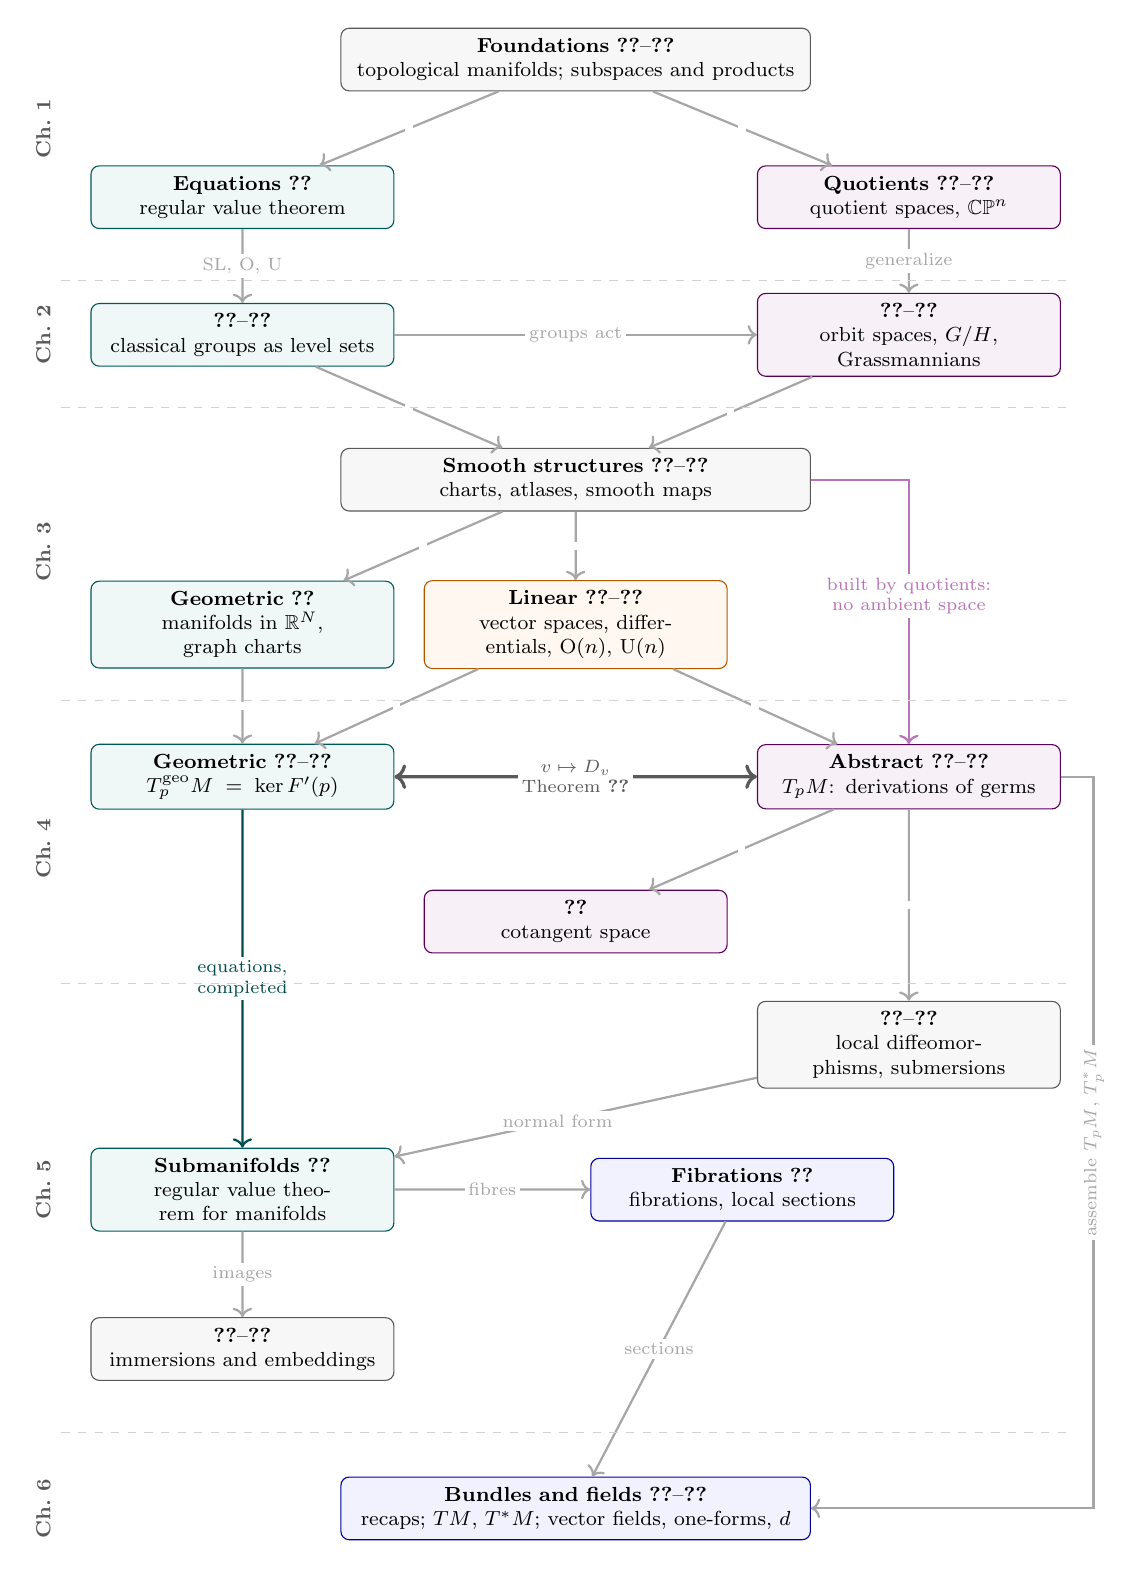
\begin{tikzpicture}[scale=0.92, transform shape]
\node[draw=gray!70!black, fill=gray!6, rounded corners=3pt, text width=6.2cm, align=center, font=\footnotesize, inner sep=4pt] (F) at (4.6,0) {\textbf{Foundations} \ref*{sec:review}--\ref*{sec:new-spaces}\\ topological manifolds; subspaces and products};
\node[draw=teal!70!black, fill=teal!6, rounded corners=3pt, text width=3.9cm, align=center, font=\footnotesize, inner sep=4pt] (E1) at (0,-1.9) {\textbf{Equations} \ref*{sec:rvt}\\ regular value theorem};
\node[draw=violet!70!black, fill=violet!6, rounded corners=3pt, text width=3.9cm, align=center, font=\footnotesize, inner sep=4pt] (Q1) at (9.2,-1.9) {\textbf{Quotients} \ref*{sec:quotient-spaces}--\ref*{sec:open-quotients}\\ quotient spaces, $\mathbb{CP}^n$};
\node[draw=teal!70!black, fill=teal!6, rounded corners=3pt, text width=3.9cm, align=center, font=\footnotesize, inner sep=4pt] (E2) at (0,-3.8) {\ref*{sec:topgroups}--\ref*{sec:classical-manifolds}\\ classical groups as level sets};
\node[draw=violet!70!black, fill=violet!6, rounded corners=3pt, text width=3.9cm, align=center, font=\footnotesize, inner sep=4pt] (Q2) at (9.2,-3.8) {\ref*{sec:actions}--\ref*{sec:GH-topology}\\ orbit spaces, $G/H$, Grassmannians};
\node[draw=gray!70!black, fill=gray!6, rounded corners=3pt, text width=6.2cm, align=center, font=\footnotesize, inner sep=4pt] (S) at (4.6,-5.8) {\textbf{Smooth structures} \ref*{sec:smooth-structures}--\ref*{sec:smooth-maps}\\ charts, atlases, smooth maps};
\node[draw=teal!70!black, fill=teal!6, rounded corners=3pt, text width=3.9cm, align=center, font=\footnotesize, inner sep=4pt] (G1) at (0,-7.8) {\textbf{Geometric} \ref*{sec:euclidean}\\ manifolds in $\mathbb{R}^N$, graph charts};
\node[draw=orange!70!black, fill=orange!6, rounded corners=3pt, text width=3.9cm, align=center, font=\footnotesize, inner sep=4pt] (L) at (4.6,-7.8) {\textbf{Linear} \ref*{sec:vector-spaces}--\ref*{sec:on-un-smooth}\\ vector spaces, differentials, $\Ogp(n)$, $\Ugp(n)$};
\node[draw=teal!70!black, fill=teal!6, rounded corners=3pt, text width=3.9cm, align=center, font=\footnotesize, inner sep=4pt] (T1) at (0,-9.9) {\textbf{Geometric} \ref*{sec:tangent}--\ref*{sec:transversality}\\ $T^{\geo}_pM = \ker F'(p)$};
\node[draw=violet!70!black, fill=violet!6, rounded corners=3pt, text width=3.9cm, align=center, font=\footnotesize, inner sep=4pt] (T2) at (9.2,-9.9) {\textbf{Abstract} \ref*{sec:abstract-tangent}--\ref*{sec:velocities}\\ $T_pM$: derivations of germs};
\node[draw=violet!70!black, fill=violet!6, rounded corners=3pt, text width=3.9cm, align=center, font=\footnotesize, inner sep=4pt] (C) at (4.6,-11.9) {\ref*{sec:cotangent}\\ cotangent space};
\node[draw=gray!70!black, fill=gray!6, rounded corners=3pt, text width=3.9cm, align=center, font=\footnotesize, inner sep=4pt] (M) at (9.2,-13.6) {\ref*{sec:special-maps}--\ref*{sec:submersions}\\ local diffeomorphisms, submersions};
\draw[->, thick, gray!70, ] (F) -- node[font=\scriptsize, fill=white, inner sep=1.5pt] {} (E1);
\draw[->, thick, gray!70, ] (F) -- node[font=\scriptsize, fill=white, inner sep=1.5pt] {} (Q1);
\draw[->, thick, gray!70, ] (E1) -- node[font=\scriptsize, fill=white, inner sep=1.5pt] {$\SL$, $\Ogp$, $\Ugp$} (E2);
\draw[->, thick, gray!70, ] (Q1) -- node[font=\scriptsize, fill=white, inner sep=1.5pt] {generalize} (Q2);
\draw[->, thick, gray!70, ] (E2) -- node[font=\scriptsize, fill=white, inner sep=1.5pt] {groups act} (Q2);
\draw[->, thick, gray!70, ] (E2) -- node[font=\scriptsize, fill=white, inner sep=1.5pt] {} (S);
\draw[->, thick, gray!70, ] (Q2) -- node[font=\scriptsize, fill=white, inner sep=1.5pt] {} (S);
\draw[->, thick, gray!70, ] (S) -- node[font=\scriptsize, fill=white, inner sep=1.5pt] {} (G1);
\draw[->, thick, gray!70, ] (S) -- node[font=\scriptsize, fill=white, inner sep=1.5pt] {} (L);
\draw[->, thick, violet!55] (S.east) -| node[pos=0.72, font=\scriptsize, fill=white, inner sep=1.5pt, align=center] {built by quotients:\\ no ambient space} (T2.north);
\draw[->, thick, gray!70, ] (G1) -- node[font=\scriptsize, fill=white, inner sep=1.5pt] {} (T1);
\draw[->, thick, gray!70, ] (L) -- node[font=\scriptsize, fill=white, inner sep=1.5pt] {} (T1);
\draw[->, thick, gray!70, ] (L) -- node[font=\scriptsize, fill=white, inner sep=1.5pt] {} (T2);
\draw[<->, very thick, black!65] (T1) -- node[font=\scriptsize, fill=white, inner sep=1.5pt, align=center] {$v \mapsto D_v$\\ Theorem~\ref*{thm:ambient-abstract}} (T2);
\draw[->, thick, gray!70, ] (T2) -- node[font=\scriptsize, fill=white, inner sep=1.5pt] {} (C);
\draw[->, thick, gray!70, ] (T2) -- node[font=\scriptsize, fill=white, inner sep=1.5pt] {} (M);
\node[font=\footnotesize\bfseries, gray!70!black, rotate=90] at (-2.75,-0.95) {Ch.~1};
\node[font=\footnotesize\bfseries, gray!70!black, rotate=90] at (-2.75,-3.8) {Ch.~2};
\node[draw=teal!70!black, fill=teal!6, rounded corners=3pt, text width=3.9cm, align=center, font=\footnotesize, inner sep=4pt] (SM) at (0,-15.6) {\textbf{Submanifolds} \ref*{sec:submanifolds}\\ regular value theorem for manifolds};
\node[draw=blue!60!black, fill=blue!5, rounded corners=3pt, text width=3.9cm, align=center, font=\footnotesize, inner sep=4pt] (BU) at (6.9,-15.6) {\textbf{Fibrations} \ref*{sec:fibrations}\\ fibrations, local sections};
\node[draw=blue!60!black, fill=blue!5, rounded corners=3pt, text width=6.2cm, align=center, font=\footnotesize, inner sep=4pt] (BF) at (4.6,-20.0) {\textbf{Bundles and fields} \ref*{sec:recap-tangent}--\ref*{sec:vf-operators}\\ recaps; $TM$, $T^*M$; vector fields, one-forms, $d$};
\draw[->, thick, gray!70] (BU) -- node[pos=0.5, font=\scriptsize, fill=white, inner sep=1.5pt] {sections} (BF);
\draw[->, thick, teal!60!black] (T1) -- node[font=\scriptsize, fill=white, inner sep=1.5pt, align=center] {equations,\\ completed} (SM);
\draw[->, thick, gray!70] (M) -- node[pos=0.55, font=\scriptsize, fill=white, inner sep=1.5pt] {normal form} (SM);
\draw[->, thick, gray!70] (SM) -- node[font=\scriptsize, fill=white, inner sep=1.5pt] {fibres} (BU);
\draw[->, thick, gray!70] (T2.east) -- ++(0.45,0) |- node[pos=0.25, font=\scriptsize, fill=white, inner sep=1.5pt, rotate=90] {assemble $T_pM$, $T_p^*M$} (BF.east);
\node[draw=gray!70!black, fill=gray!6, rounded corners=3pt, text width=3.9cm, align=center, font=\footnotesize, inner sep=4pt] (IM) at (0,-17.8) {\ref*{sec:immersions}--\ref*{sec:embeddings}\\ immersions and embeddings};
\draw[->, thick, gray!70] (SM) -- node[pos=0.5, font=\scriptsize, fill=white, inner sep=1.5pt] {images} (IM);
\node[font=\footnotesize\bfseries, gray!70!black, rotate=90] at (-2.75,-6.8) {Ch.~3};
\node[font=\footnotesize\bfseries, gray!70!black, rotate=90] at (-2.75,-10.9) {Ch.~4};
\node[font=\footnotesize\bfseries, gray!70!black, rotate=90] at (-2.75,-15.6) {Ch.~5};
\node[font=\footnotesize\bfseries, gray!70!black, rotate=90] at (-2.75,-20.0) {Ch.~6};
\draw[gray!35, dashed] (-2.5,-18.95) -- (11.4,-18.95);
\draw[gray!35, dashed] (-2.5,-3.05) -- (11.4,-3.05);
\draw[gray!35, dashed] (-2.5,-4.8) -- (11.4,-4.8);
\draw[gray!35, dashed] (-2.5,-8.85) -- (11.4,-8.85);
\draw[gray!35, dashed] (-2.5,-12.75) -- (11.4,-12.75);
\end{tikzpicture}
\end{center}

The labels on the arrows are the bridges. The regular value theorem (\ref{sec:rvt}) turns equations into manifolds, and graph charts (Proposition~\ref{prop:level-set-smooth}) make them smooth. The differential between vector spaces (\ref{sec:vs-differential}) gives $T^{\geo}_pM = \ker F'(p)$ (Theorem~\ref{thm:tangent-kernel}). For the quotient-built manifolds, atlases are written down by hand (\ref{sec:projective-smooth}), and only the abstract tangent space reaches them. The two tangent spaces are identified by $v \mapsto D_v$ (Theorem~\ref{thm:ambient-abstract}); the abstract differential agrees with the Jacobian (Proposition~\ref{prop:differential-agree}), and on any manifold the matrix of $F_{*p}$ in coordinates \emph{is} the Jacobian of the coordinate representation (Theorem~\ref{lem:differential-matrix}), because partial derivatives upstairs are defined downstairs (Proposition~\ref{prop:upstairs-downstairs}); and every abstract tangent vector is a velocity after all (Theorem~\ref{thm:every-vector-velocity}). At the bottom, the submersion normal form (Theorem~\ref{thm:submersion-normal-form}) proves the regular value theorem for manifolds (Theorem~\ref{thm:rvt-manifolds}), where the equations thread ends; fibrations and the tangent and cotangent spaces follow as bundles (\ref{sec:fibrations}--\ref{sec:tangent-bundle}); and immersions, whose normal form is the twin of the submersion normal form, have images that are locally submanifolds (\ref{sec:immersions}), and globally so when they are embeddings (\ref{sec:embeddings}). Each section opens with a line placing it on this map.


\part{Topological and Smooth Manifolds}

\chapter{Topological Manifolds}

% ============================================================================
% Lecture 1 (Mon Aug 31, 2026)
% SECTION 1: POINT-SET TOPOLOGY REVIEW
% ============================================================================
\section{Point-Set Topology Review}\label{sec:review}

\roadmark{Foundations}{The point-set tools that every later construction draws on.}

\textit{Reference: Lee Appendix A; MATH 590 notes \S2 (bases), \S8 (Hausdorff), \S18 (countability axioms).}

\begin{rembox}[Purpose of this Section]\label{rem:purpose-this-section}
This is a reminder, not a first exposure. The point is twofold: (i) recall the two point-set conditions that will be imposed on every manifold (second countability and the Hausdorff property), and (ii) fix the \emph{terminology} used in this course, which differs in small ways from Munkres. Throughout, $X$ denotes a topological space; the topology itself will usually not be given a name.
\end{rembox}

\subsection{Bases and Neighborhoods}

\begin{defbox}[Basis]\deflabel{def:basis}
A \textbf{basis} for $X$ is a collection $(U_\alpha)_{\alpha \in A}$ of open subsets of $X$ such that
\[
\forall\, p \in X,\ \forall\, U \text{ open with } p \in U,\ \exists\, \alpha \in A \text{ such that } p \in U_\alpha \subseteq U.
\]
\leeref{App.~A, \emph{Topological Spaces}}
\end{defbox}

\begin{propbox}[Equivalent Formulation of a Basis]\thmlabel{prop:basis-equiv}
Let $(U_\alpha)_{\alpha \in A}$ be a collection of open subsets of $X$. The following are equivalent:
\begin{enumerate}
    \item $(U_\alpha)_{\alpha \in A}$ is a basis for $X$;
    \item for every open set $U \subseteq X$ there exists a subset $A_U \subseteq A$ such that $U = \bigcup_{\alpha \in A_U} U_\alpha$.
\end{enumerate}
In words: \emph{every open set is a union of basis elements.}
\leeref{App.~A, \emph{Topological Spaces}}
\end{propbox}

\begin{proof}[Proof (not given in lecture)]
$(1 \Rightarrow 2)$ Let $U$ be open. For each $p \in U$ choose $\alpha_p \in A$ with $p \in U_{\alpha_p} \subseteq U$, and set $A_U = \{\alpha_p \mid p \in U\}$. Then $\bigcup_{\alpha \in A_U} U_\alpha \subseteq U$ since each $U_{\alpha_p} \subseteq U$, and $U \subseteq \bigcup_{\alpha \in A_U} U_\alpha$ since $p \in U_{\alpha_p}$ for every $p \in U$.

$(2 \Rightarrow 1)$ Let $p \in U$ with $U$ open. Write $U = \bigcup_{\alpha \in A_U} U_\alpha$. Since $p \in U$, there is some $\alpha \in A_U$ with $p \in U_\alpha$, and $U_\alpha \subseteq U$ by construction.
\end{proof}

\begin{rembox}[Two Notions of ``Basis'']\label{rem:two-notions-basis}
Definition~\ref{def:basis} assumes the $U_\alpha$ are already open in a \emph{given} topology on $X$: it answers the question ``when is a family of open sets a basis \emph{for} this topology?'' In 590 (Munkres \S13) the word ``basis'' was used in a different, generative sense: one starts from a bare set $X$ and an abstract collection $\mathcal{B}$ of subsets satisfying two axioms, and \emph{builds} a topology out of $\mathcal{B}$. We record that definition next and then show the two notions agree.
\end{rembox}

\begin{defbox}[Basis for a Topology --- Alternate Definition from MATH 590]\deflabel{def:basis-alt}
If $X$ is a set, a \textbf{basis for a topology on $X$} is a collection $\mathcal{B}$ of subsets of $X$ (called \textbf{basis elements}) such that:
\begin{enumerate}
    \item For each $x \in X$, there exists at least one basis element $B \in \mathcal{B}$ containing $x$.
    \item If $x \in B_1 \cap B_2$, where $B_1, B_2 \in \mathcal{B}$, then there exists $B_3 \in \mathcal{B}$ containing $x$ such that $B_3 \subseteq B_1 \cap B_2$.
\end{enumerate}
Given such a $\mathcal{B}$, the \textbf{topology $\mathcal{T}_{\mathcal{B}}$ generated by $\mathcal{B}$} is defined by: $U \subseteq X$ is open if for every $x \in U$ there exists $B \in \mathcal{B}$ with $x \in B \subseteq U$. Equivalently (590 Lemma 2.1), $\mathcal{T}_{\mathcal{B}}$ is the collection of all unions of elements of $\mathcal{B}$.
\leeref{App.~A, \emph{Topological Spaces}}
\end{defbox}

\begin{propbox}[The Two Definitions of Basis Agree]\thmlabel{prop:two-definitions-basis-agree}
Let $X$ be a set and $\mathcal{B}$ a collection of subsets of $X$.
\begin{enumerate}
    \item[(a)] If $\mathcal{B}$ satisfies Definition~\ref{def:basis-alt}, then every $B \in \mathcal{B}$ is open in $\mathcal{T}_{\mathcal{B}}$, and $\mathcal{B}$ is a basis for the topological space $(X, \mathcal{T}_{\mathcal{B}})$ in the sense of Definition~\ref{def:basis}.
    \item[(b)] Conversely, if $\mathcal{T}$ is a topology on $X$ and $\mathcal{B} \subseteq \mathcal{T}$ is a basis for $(X, \mathcal{T})$ in the sense of Definition~\ref{def:basis}, then $\mathcal{B}$ satisfies the two axioms of Definition~\ref{def:basis-alt}, and the topology it generates is $\mathcal{T}_{\mathcal{B}} = \mathcal{T}$.
\end{enumerate}
\end{propbox}

\begin{proof}[Proof (not given in lecture)]
(a) That $\mathcal{T}_{\mathcal{B}}$ is a topology was proved in 590 \S2 (axiom 2 is exactly what makes finite intersections open). For $B \in \mathcal{B}$ and $x \in B$, the element $B$ itself witnesses $x \in B \subseteq B$, so $B \in \mathcal{T}_{\mathcal{B}}$. Now let $p \in U$ with $U \in \mathcal{T}_{\mathcal{B}}$; by the very definition of $\mathcal{T}_{\mathcal{B}}$ there is $B \in \mathcal{B}$ with $p \in B \subseteq U$, which is the condition in Definition~\ref{def:basis}.

(b) \emph{Axiom 1:} $X \in \mathcal{T}$ is open, so for $x \in X$ Definition~\ref{def:basis} gives $B \in \mathcal{B}$ with $x \in B \subseteq X$. \emph{Axiom 2:} if $B_1, B_2 \in \mathcal{B} \subseteq \mathcal{T}$, then $B_1 \cap B_2 \in \mathcal{T}$ (finite intersection), so for $x \in B_1 \cap B_2$ Definition~\ref{def:basis} gives $B_3 \in \mathcal{B}$ with $x \in B_3 \subseteq B_1 \cap B_2$.

\emph{$\mathcal{T}_{\mathcal{B}} = \mathcal{T}$:} If $U \in \mathcal{T}$, then for each $x \in U$ there is $B \in \mathcal{B}$ with $x \in B \subseteq U$ (Definition~\ref{def:basis}), so $U \in \mathcal{T}_{\mathcal{B}}$. If $U \in \mathcal{T}_{\mathcal{B}}$, then $U = \bigcup_{x \in U} B_x$ with each $B_x \in \mathcal{B} \subseteq \mathcal{T}$, so $U \in \mathcal{T}$ (arbitrary union of open sets).
\end{proof}

\begin{rembox}[Which Definition to Use When]\label{rem:which-definition-use-when}
The proposition says ``basis'' has a single meaning; the two definitions are just the two directions of use.
\begin{itemize}
    \item \textbf{Topology already given} (e.g.\ $\mathbb{R}^n$ with the usual topology, or a subspace of it): use Definition~\ref{def:basis} to \emph{verify} that a proposed family is a basis. This is what the second-countability examples below do.
    \item \textbf{Topology to be constructed} (e.g.\ the line with two origins, product and quotient topologies): use Definition~\ref{def:basis-alt} to \emph{generate} it from a convenient family $\mathcal{B}$, after checking axiom 2. Uribe phrases this as ``it suffices to give a basis of neighborhoods of each point,'' which is Definition~\ref{def:basis-alt} applied to the union of the local bases.
\end{itemize}
Uribe stated Definition~\ref{def:basis} and the reformulation in Proposition~\ref{prop:basis-equiv}; Definition~\ref{def:basis-alt} was not written in lecture but is the form used implicitly whenever a topology is specified by a basis.
\end{rembox}

\begin{defbox}[Neighborhood]\deflabel{def:neighborhood}
A \textbf{neighborhood} (abbreviated \textbf{nbhd}) of a point $p \in X$ is any \emph{open} set $U$ with $p \in U$.
\end{defbox}

\begin{rembox}[Terminology Warning: All Neighborhoods Are Open]\label{rem:terminology-warning-all-neighborhoods-open}
In this course (and in Lee), a neighborhood of $p$ is by definition an \emph{open} set containing $p$. Some texts (e.g.\ in analysis, or Bourbaki) call any set containing an open set around $p$ a neighborhood. Munkres and 590 used the open convention as well, so nothing changes for us---but check the convention whenever reading a new book.
\end{rembox}

\begin{defbox}[Basis of Neighborhoods at a Point]\deflabel{def:local-basis}
A \textbf{basis of neighborhoods} (or \textbf{local basis}) of $p \in X$ is a collection $(V_\alpha)_{\alpha \in A_p}$ of neighborhoods of $p$ such that
\[
\forall\, U \text{ nbhd of } p,\ \exists\, \alpha \in A_p \text{ such that } V_\alpha \subseteq U.
\]
\leeref{App.~A, \emph{Topological Spaces} (``neighborhood basis)}
\end{defbox}

\begin{propbox}[Global and Local Bases]\thmlabel{prop:global-local-bases}
Let $X$ be a topological space.
\begin{enumerate}
    \item If $(U_\alpha)_{\alpha \in A}$ is a basis for $X$ and $p \in X$, then $\{U_\alpha \mid \alpha \in A,\ p \in U_\alpha\}$ is a basis of neighborhoods of $p$.
    \item Conversely, if for each $p \in X$ a basis of neighborhoods $\mathcal{B}_p$ of $p$ is given, then $\bigcup_{p \in X}\mathcal{B}_p$ is a basis for $X$.
\end{enumerate}
\leeref{App.~A, \emph{Topological Spaces}}
\end{propbox}

\begin{proof}
(1) Given a neighborhood $U$ of $p$, Definition~\ref{def:basis} supplies $\alpha$ with $p \in U_\alpha \subseteq U$. (2) Every member of $\bigcup_p \mathcal{B}_p$ is open. If $U$ is open and $p \in U$, then $U$ is a neighborhood of $p$, so some $B \in \mathcal{B}_p$ has $p \in B \subseteq U$; this is Definition~\ref{def:basis}.
\end{proof}

\begin{rembox}\label{rem:review}
Part (2), read through Definition~\ref{def:basis-alt}, is why it suffices to \emph{define} a topology by specifying a basis of neighborhoods at every point --- provided the family satisfies the intersection axiom there. This is how the line with two origins is defined below.
\end{rembox}

\subsection{Second Countability}

\begin{defbox}[Second Countable]\deflabel{def:second-countable}
$X$ is \textbf{second countable} if there exists a basis $\{U_\alpha\}_{\alpha \in A}$ of $X$ such that the index set $A$ is countable.
\end{defbox}

\begin{rembox}[Why Second Countability?]\label{rem:why-second-countability}
Second countability is the first of the three conditions defining a manifold. Its job is to keep the space from being ``too big.'' Concretely, it is what makes \emph{partitions of unity} possible later in the course (via paracompactness), and it forces a manifold to have only countably many connected components (Proposition~\ref{prop:count-components}). Compare 590 \S18, where second countability was the hypothesis of the Urysohn metrization theorem.
\end{rembox}

\begin{exbox}[$\mathbb{R}^n$ with the Usual Topology is Second Countable]\exlabel{ex:rn-2c}
A countable basis is
\[
\{B_{\alpha, r}\}_{\alpha \in \mathbb{Q}^n,\ r \in \mathbb{Q}_{>0}}, \qquad B_{\alpha, r} = \{x \in \mathbb{R}^n \mid |x - \alpha| < r\},
\]
i.e.\ all open balls with rational center and rational radius. The index set $\mathbb{Q}^n \times \mathbb{Q}_{>0} \subseteq \mathbb{Q}^{n+1}$ is countable.
\leeref{App.~A, \emph{Topological Spaces}}
\end{exbox}

\begin{proof}[Proof that this is a basis (not given in lecture)]
Let $U \subseteq \mathbb{R}^n$ be open and $x \in U$. Choose $\varepsilon > 0$ with $B(x, \varepsilon) \subseteq U$. By density of $\mathbb{Q}^n$ in $\mathbb{R}^n$, pick $\alpha \in \mathbb{Q}^n$ with $|x - \alpha| < \varepsilon/3$, and pick $r \in \mathbb{Q}$ with $\varepsilon/3 < r < 2\varepsilon/3$. Then:
\begin{itemize}
    \item $x \in B_{\alpha, r}$, since $|x - \alpha| < \varepsilon/3 < r$;
    \item $B_{\alpha, r} \subseteq B(x, \varepsilon) \subseteq U$: if $|y - \alpha| < r$, then $|y - x| \le |y - \alpha| + |\alpha - x| < r + \varepsilon/3 < \varepsilon$.
\end{itemize}
Hence every open $U$ containing $x$ contains a basis element containing $x$.
\end{proof}

\begin{exbox}[Non-Example: $\mathbb{R}$ with the Discrete Topology]\exlabel{ex:r-discrete}
Let $X = \mathbb{R}$ with the discrete topology, so every subset (in particular every singleton $\{x\}$) is open. Then $X$ is \emph{not} second countable.

\textit{Reason:} let $\{U_\alpha\}$ be any basis. For each $x \in \mathbb{R}$, the open set $\{x\}$ contains $x$, so some $U_\alpha$ satisfies $x \in U_\alpha \subseteq \{x\}$, i.e.\ $U_\alpha = \{x\}$. Thus the basis contains every singleton, and $\mathbb{R}$ is uncountable.
\leeref{Example A.4}
\end{exbox}

\begin{defbox}[First Countable at a Point]\deflabel{def:first-countable}
$X$ is \textbf{first countable at $x_0 \in X$} if there is a countable basis of neighborhoods of $x_0$ (Definition~\ref{def:local-basis}); $X$ is \textbf{first countable} if it is first countable at each of its points.
\leeref{App.~A, \emph{Topological Spaces}}
\end{defbox}

\begin{propbox}[Second Countable Implies First Countable]\thmlabel{prop:2c-implies-1c}
A second countable space is first countable at each of its points.
\leeref{App.~A, \emph{Topological Spaces}}
\end{propbox}

\begin{proof}
Let $\mathcal{B}$ be a countable basis of $X$ and $x_0 \in X$. Put $\mathcal{B}_{x_0} = \{\, B \in \mathcal{B} \mid x_0 \in B \,\}$, a countable collection since $\mathcal{B}$ is. Each of its members is a neighborhood of $x_0$. If $U$ is any neighborhood of $x_0$, then by Definition~\ref{def:basis} there is $B \in \mathcal{B}$ with $x_0 \in B \subseteq U$, and such a $B$ lies in $\mathcal{B}_{x_0}$. So $\mathcal{B}_{x_0}$ is a countable basis of neighborhoods of $x_0$.
\end{proof}

\begin{rembox}\label{rem:review-2}
The contrapositive is the useful direction: to prove a space is \emph{not} second countable it suffices to exhibit one point at which it is not first countable. That is how Example~\ref{ex:not-2c-quotient} below shows a quotient of $\mathbb{R}$ fails second countability. The converse of the proposition is false: $\mathbb{R}$ with the discrete topology (Example~\ref{ex:r-discrete}) is first countable---$\{\{x\}\}$ is a one-element basis of neighborhoods at $x$---but not second countable.
\end{rembox}

\subsection{Hausdorff Spaces}

\begin{defbox}[Hausdorff ($T_2$)]\deflabel{def:hausdorff-t2}
$X$ is \textbf{Hausdorff} (or $T_2$) if
\[
\forall\, p, q \in X \text{ with } p \neq q,\ \exists\, U \text{ nbhd of } p,\ V \text{ nbhd of } q \text{ such that } U \cap V = \emptyset.
\]
That is, distinct points can be separated by neighborhoods.
\end{defbox}

\begin{rembox}\label{rem:review-3}
There is a whole hierarchy of separation axioms ($T_0, T_1, T_{2\frac12}, T_3, T_{3\frac12}, \ldots$; see 590 \S19). Uribe's editorial: learning all of them is mostly a waste of time. For manifolds, $T_2$ is the one that matters.
\end{rembox}

\begin{exbox}[Any Metric Space is $T_2$]\exlabel{ex:metric-t2}
Let $d : X \times X \to \mathbb{R}$ be a metric and $p \neq q$. Put $r = \tfrac13 d(p, q) > 0$ and take
\[
U = B(p, r) = \{x \mid d(p, x) < r\}, \qquad V = B(q, r).
\]
Then $U \cap V = \emptyset$: if $z \in U \cap V$, the triangle inequality gives
\[
d(p, q) \le d(p, z) + d(z, q) < r + r = \tfrac23 d(p, q),
\]
which is impossible since $d(p,q) > 0$.
This is the argument given on the board in Lecture~1.
\leeref{Example A.5}
\end{exbox}
\begin{center}
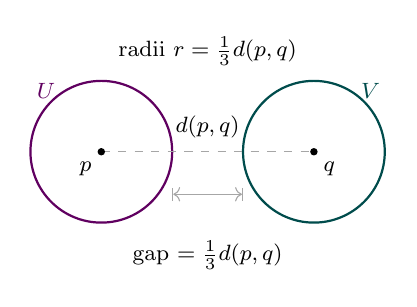
\begin{tikzpicture}[scale=0.9]
\draw[violet!75!black,thick] (0,0) circle (1);
\draw[teal!60!black,thick] (3,0) circle (1);
\draw[dashed,gray!70] (0,0) -- (3,0);
\fill (0,0) circle (1.5pt) node[font=\footnotesize,below left]{$p$};
\fill (3,0) circle (1.5pt) node[font=\footnotesize,below right]{$q$};
\node[font=\footnotesize,above] at (1.5,0.06) {$d(p,q)$};
\draw[|<->|,gray!70] (1,-0.6) -- (2,-0.6);
\node[font=\footnotesize,below] at (1.5,-1.12) {gap $=\tfrac13 d(p,q)$};
\node[violet!75!black,font=\footnotesize] at (-0.78,0.86) {$U$};
\node[teal!60!black,font=\footnotesize] at (3.8,0.86) {$V$};
\node[font=\footnotesize] at (1.5,1.42) {radii $r=\tfrac13 d(p,q)$};
\end{tikzpicture}
\end{center}


\begin{exbox}[Non-Example: The Real Line with Two Origins]\exlabel{ex:two-origins}
As a \emph{set}, let
\[
X = (-\infty, 0) \cup \{0_1, 0_2\} \cup (0, +\infty),
\]
where $0_1, 0_2$ are two distinct points (and the ordinary $0$ is absent). Picture: a left ray, a right ray, and two ``origins'' sitting side by side at the gap.

\textit{Topology.} The open sets contained in $(-\infty, 0)$ or in $(0, \infty)$ are the usual ones. A basis of neighborhoods of $0_i$ ($i = 1, 2$) is
\[
\big\{ (-\varepsilon, 0) \cup \{0_i\} \cup (0, \varepsilon) \big\}_{\varepsilon \in \mathbb{R}_{>0}}.
\]
Precisely: write $N_i(\varepsilon) = (-\varepsilon, 0) \cup \{0_i\} \cup (0, \varepsilon)$ and let
\[
\mathcal{B} = \{\, (a,b) \mid a < b \le 0 \text{ or } 0 \le a < b \,\} \;\cup\; \{\, N_1(\varepsilon) \mid \varepsilon > 0 \,\} \;\cup\; \{\, N_2(\varepsilon) \mid \varepsilon > 0 \,\},
\]
the open intervals contained in one of the rays together with the punctured neighborhoods of the two origins. The topology of $X$ is $\mathcal{T}_{\mathcal{B}}$, the topology generated by $\mathcal{B}$ (Definition~\ref{def:basis-alt}). For this to make sense, $\mathcal{B}$ must satisfy the two axioms.

\emph{Axiom 1.} A point $x < 0$ lies in $(x - 1, x/2) \in \mathcal{B}$, a point $x > 0$ lies in $(x/2, x + 1) \in \mathcal{B}$, and the origin $0_i$ lies in $N_i(1)$.

\emph{Axiom 2.} It suffices to show that the intersection of any two members of $\mathcal{B}$ is a union of members of $\mathcal{B}$ (then any $x$ in the intersection lies in one of those members, which is contained in the intersection). There are four cases, with $m = \min(\varepsilon, \delta)$:
\begin{itemize}
    \item $(a,b) \cap (c,d)$ is an open interval contained in a ray, or empty (the empty union).
    \item $N_i(\varepsilon) \cap N_i(\delta) = N_i(m) \in \mathcal{B}$.
    \item $N_1(\varepsilon) \cap N_2(\delta) = (-m, 0) \cup (0, m)$, a union of two intervals in $\mathcal{B}$ (the origins $0_1 \neq 0_2$ are distinct points, so neither survives).
    \item $N_i(\varepsilon) \cap (a,b)$: since $(a,b)$ lies in one ray, this equals $(a,b) \cap (-\varepsilon, 0)$ or $(a,b) \cap (0, \varepsilon)$, an interval in that ray or empty.
\end{itemize}

\emph{Consequences.} (i) An open set contained in a ray is a union of members of $\mathcal{B}$ none of which can be an $N_i(\varepsilon)$ (those contain an origin), hence a union of intervals in that ray: the open subsets of each ray are the usual ones. (ii) $\{N_i(\varepsilon)\}_{\varepsilon > 0}$ is a basis of neighborhoods of $0_i$: if $W$ is open and $0_i \in W$, then $W$ is a union of members of $\mathcal{B}$, and the only members containing $0_i$ are the $N_i(\varepsilon)$, so some $N_i(\varepsilon) \subseteq W$.

\textit{$X$ is not Hausdorff.} Any neighborhood of $0_1$ contains a basic set $(-\varepsilon_1, 0) \cup \{0_1\} \cup (0, \varepsilon_1)$, and any neighborhood of $0_2$ contains a basic set $(-\varepsilon_2, 0) \cup \{0_2\} \cup (0, \varepsilon_2)$. Both contain $(-\min(\varepsilon_1, \varepsilon_2), 0) \neq \emptyset$. So $0_1$ and $0_2$ cannot be separated.
\leeref{Problem 1-1}
\end{exbox}

\textit{Provenance.} Lecture~1 gave the set, the neighbourhood bases of $0_1$ and $0_2$, and the verdict ``you cannot separate the two origins.'' It sketched the other two conditions in words: second countability (``I won't prove [it] \ldots\ each one has a countable basis'') and local Euclideanness (``there's an obvious bijection with $(-\varepsilon, \varepsilon)$, and this turns out to be a homeomorphism''). The verification above that the proposed sets form a basis, and the precise non-separation argument, are filled in.
\begin{center}
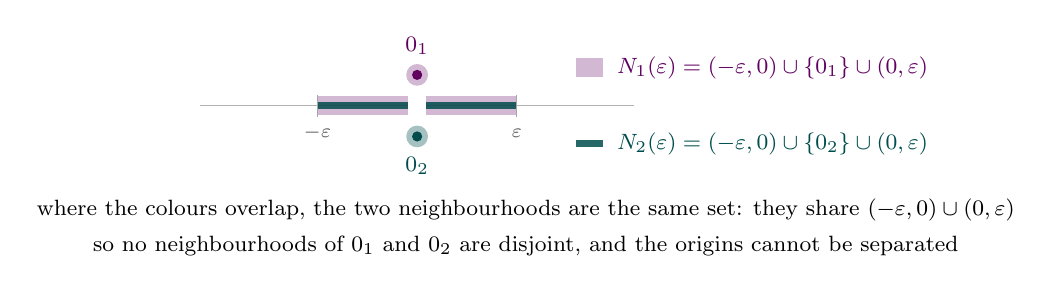
\begin{tikzpicture}[scale=1.15]
% the line, with no ordinary origin
\draw[gray!60] (-2.4,0) -- (-0.1,0); \draw[gray!60] (0.1,0) -- (2.4,0);
% both neighbourhoods painted on the SAME punctured interval: wide purple band, narrow teal band on top
\draw[violet!75!black, line width=7pt, opacity=0.28] (-1.1,0) -- (-0.1,0); \draw[violet!75!black, line width=7pt, opacity=0.28] (0.1,0) -- (1.1,0);
\draw[teal!60!black, line width=2.4pt, opacity=0.85] (-1.1,0) -- (-0.1,0); \draw[teal!60!black, line width=2.4pt, opacity=0.85] (0.1,0) -- (1.1,0);
% the two origins at the gap, each in its own neighbourhood's colour
\fill[violet!75!black, opacity=0.28] (0,0.34) circle (0.12); \fill[violet!75!black] (0,0.34) circle (1.6pt);
\node[violet!75!black,font=\footnotesize,above] at (0,0.46) {$0_1$};
\fill[teal!60!black, opacity=0.35] (0,-0.34) circle (0.12); \fill[teal!60!black] (0,-0.34) circle (1.6pt);
\node[teal!60!black,font=\footnotesize,below] at (0,-0.46) {$0_2$};
% the scale epsilon
\draw[gray!70] (-1.1,-0.12) -- (-1.1,0.12); \draw[gray!70] (1.1,-0.12) -- (1.1,0.12);
\node[font=\scriptsize, text=gray!70!black] at (-1.1,-0.3) {$-\varepsilon$}; \node[font=\scriptsize, text=gray!70!black] at (1.1,-0.3) {$\varepsilon$};
% legend
\draw[violet!75!black, line width=7pt, opacity=0.28] (1.75,0.42) -- (2.05,0.42); \node[violet!75!black,font=\footnotesize,anchor=west] at (2.1,0.42) {$N_1(\varepsilon) = (-\varepsilon,0)\cup\{0_1\}\cup(0,\varepsilon)$};
\draw[teal!60!black, line width=2.4pt, opacity=0.85] (1.75,-0.42) -- (2.05,-0.42); \node[teal!60!black,font=\footnotesize,anchor=west] at (2.1,-0.42) {$N_2(\varepsilon) = (-\varepsilon,0)\cup\{0_2\}\cup(0,\varepsilon)$};
\node[font=\footnotesize] at (1.2,-1.15) {where the colours overlap, the two neighbourhoods are the same set: they share $(-\varepsilon,0)\cup(0,\varepsilon)$};
\node[font=\footnotesize] at (1.2,-1.55) {so no neighbourhoods of $0_1$ and $0_2$ are disjoint, and the origins cannot be separated};
\end{tikzpicture}
\end{center}


\begin{rembox}[The Line with Two Origins as a Quotient]\label{rem:line-two-origins-quotient}
Equivalently (Proposition~\ref{prop:two-origins-agree}), $X$ is the quotient of $\mathbb{R} \times \{1, 2\}$ (two disjoint copies of $\mathbb{R}$) by the equivalence relation $(x, 1) \sim (x, 2)$ for all $x \neq 0$: glue the two lines everywhere except at the origins. This is the standard example showing that \emph{a quotient of a Hausdorff space need not be Hausdorff} (cf.\ 590 \S12). We will meet this space again in \ref{sec:manifolds} as the reason the Hausdorff condition must be imposed \emph{separately} on manifolds---it does not follow from being locally Euclidean.
\end{rembox}


\subsection{Standing Facts Imported from MATH 590}

\begin{rembox}\label{rem:review-4}
The following results from point-set topology are used in these notes without further comment. They are stated here so the notes are self-contained; proofs are in the MATH 590 notes at the sections indicated, except for the two items marked $(\ast)$, which were not recorded there and are proved below.
\end{rembox}

\begin{propbox}[Continuity and Homeomorphisms]\thmlabel{fact:cont}
Let $X, Y$ be topological spaces.
\begin{enumerate}
    \item $(\ast)$ If $\mathcal{B}$ is a basis for $Y$, then $f : X \to Y$ is continuous if and only if $f^{-1}(B)$ is open in $X$ for every $B \in \mathcal{B}$.
    \item A bijection $f : X \to Y$ is a homeomorphism if and only if, for every $U \subseteq X$, $U$ is open in $X$ $\iff$ $f(U)$ is open in $Y$. In particular, homeomorphisms are open maps. \hfill (590 \S9)
    \item If $f : X \to Y$ is a homeomorphism and $A \subseteq X$, then $f|_A : A \to f(A)$ is a homeomorphism for the subspace topologies; if moreover $A$ is open in $X$, then $f(A)$ is open in $Y$. \hfill (590 \S9)
    \item A map $F : Z \to X \times Y$ is continuous if and only if $\pi_X \circ F$ and $\pi_Y \circ F$ are continuous. \hfill (590 \S9; also Theorem~\ref{thm:univ-product})
\end{enumerate}
\leeref{Lemma A.19 and App.~A, \emph{Topological Spaces}}
\end{propbox}

\begin{proof}[Proof of (1)]
If $f$ is continuous, preimages of the (open) basis elements are open. Conversely, every open $V \subseteq Y$ is a union $V = \bigcup_i B_i$ of basis elements (Proposition~\ref{prop:basis-equiv}), and $f^{-1}(V) = \bigcup_i f^{-1}(B_i)$ is a union of open sets.
\end{proof}

\begin{proof}[Proof (to be filled)]
Parts (2)--(4) are proved in MATH 590 (\S9; see the Topology notes); to be filled.
\end{proof}

\begin{propbox}[Metric Spaces]\thmlabel{fact:metric}
Let $(X, d)$ be a metric space with the metric topology.
\begin{enumerate}
    \item $X$ is Hausdorff. \hfill (590 \S11; Example~\ref{ex:metric-t2})
    \item For $A \subseteq X$, the subspace topology on $A$ coincides with the metric topology of the restricted metric $d|_{A \times A}$; in particular every subspace of a metric space is metrizable. \hfill (590 \S11)
    \item $X$ is second countable if and only if it is separable (has a countable dense subset). In particular $\mathbb{R}^n$, and hence every subspace of $\mathbb{R}^n$, is second countable. \hfill (590 \S18; Example~\ref{ex:rn-2c})
\end{enumerate}
\leeref{Example A.5}
\end{propbox}

\begin{proof}[Proof (to be filled)]
Proved in MATH 590 (\S11 and \S18; see the Topology notes); to be filled.
\end{proof}

\begin{defbox}[Connected Component]\deflabel{def:component}
Let $X$ be a topological space and $p \in X$. The \textbf{connected component} of $p$ is the union of all connected subsets of $X$ containing $p$.
\leeref{App.~A, \emph{Connectedness and Compactness}}
\end{defbox}

\begin{propbox}[Connectedness and Components]\thmlabel{fact:conn}
Let $X$ be a topological space, and components be as in Definition~\ref{def:component}.
\begin{enumerate}
    \item The continuous image of a connected space is connected. \hfill (590 \S13)
    \item A union of connected subspaces having a point in common is connected. \hfill (590 \S13)
    \item $(\ast)$ The component of $p$ is connected, and the components of $X$ partition $X$: two components are either equal or disjoint.
    \item $\mathbb{R}^n$ and its open balls are connected; hence any space homeomorphic to one of them is connected. \hfill (590 \S14, by (1))
\end{enumerate}
\leeref{Propositions A.39, A.41 and A.43}
\end{propbox}

\begin{proof}[Proof of (3)]
Let $C_p$ be the component of $p$. Every connected set containing $p$ contains $p$, so by (2) their union $C_p$ is connected. Now suppose $C_p \cap C_q \neq \emptyset$. Then $C_p \cup C_q$ is a union of two connected sets with a common point, hence connected by (2); it contains $p$, so $C_p \cup C_q \subseteq C_p$, i.e.\ $C_q \subseteq C_p$. Symmetrically $C_p \subseteq C_q$. Since every $p$ lies in $C_p$, the components cover $X$.
\end{proof}

\begin{proof}[Proof (to be filled)]
Parts (1), (2) and (4) are proved in MATH 590 (\S13--\S14; see the Topology notes); to be filled.
\end{proof}

\begin{propbox}[Compactness]\thmlabel{fact:compact}
\begin{enumerate}
    \item (Heine--Borel) A subset of $\mathbb{R}^n$ is compact if and only if it is closed and bounded. \hfill (590 \S15)
    \item The continuous image of a compact space is compact. \hfill (590 \S15)
    \item A finite product of compact spaces is compact. \hfill (590 \S15)
    \item A compact subspace of a Hausdorff space is closed. \hfill (590 \S15)
    \item A closed subset of a compact space is compact. \hfill (590 \S15)
    \item A continuous bijection from a compact space onto a Hausdorff space is a homeomorphism. \hfill (590 \S15; proof: by (5), (2), (4) it is a closed map)
\end{enumerate}
\leeref{Propositions A.45 and A.50, Lemma A.52}
\end{propbox}

\begin{proof}[Proof (to be filled)]
Proved in MATH 590 (\S15; see the Topology notes); to be filled.
\end{proof}

% ============================================================================
% SECTION 2: TOPOLOGICAL MANIFOLDS
% ============================================================================
\section{Topological Manifolds}\label{sec:manifolds}

\roadmark{Foundations}{The definition of a topological manifold and the role of each axiom. The two ways of building examples begin next: by quotients (\ref{sec:quotient-spaces}--\ref{sec:open-quotients}) and by equations (\ref{sec:rvt}).}

\textit{Reference: Lee Ch.\ 1, ``Topological Manifolds.''}

\subsection{The Definition}

\begin{defbox}[Locally Euclidean]\deflabel{def:locally-euclidean}
$X$ is \textbf{locally Euclidean} (of dimension $n$) if there exists $n \in \mathbb{N}$ such that for every $p \in X$ there exist a neighborhood $U$ of $p$ and a map
\[
\varphi : U \longrightarrow \mathbb{R}^n
\]
which is a \textbf{homeomorphism}: $\varphi$ is continuous, bijective, and $\varphi^{-1} : \mathbb{R}^n \to U$ is also continuous.
\end{defbox}

\begin{rembox}[Quantifier Order]\label{rem:quantifier-order}
As first written on the board, the definition read ``$\forall p\ \exists U\ \exists \varphi: U \to \mathbb{R}^n$,'' with $n$ implicitly fixed. A student asked whether $n$ is allowed to depend on $p$; the answer in this course is \textbf{no}: ``$\exists n$'' comes \emph{before} ``$\forall p$.'' See the remark ``Conventions on the Dimension'' below for what happens under the other convention.
\end{rembox}

\begin{defbox}[Topological Manifold]\deflabel{def:manifold}
A \textbf{topological manifold} (of dimension $n$) is a topological space $X$ that is
\begin{enumerate}
    \item second countable,
    \item Hausdorff ($T_2$), and
    \item locally Euclidean of dimension $n$.
\end{enumerate}
\leeref{Ch.~1, \emph{Topological Manifolds}}
\end{defbox}

\begin{rembox}[Why These Three Conditions?]\label{rem:why-these-three-conditions}
Locally Euclidean is the substantive geometric condition: near every point the space looks like $\mathbb{R}^n$, so calculus can (eventually) be imported chart by chart. The other two are global point-set hygiene. Hausdorff rules out non-uniqueness of limits (and, later, guarantees that compact subsets are closed, that one-point sets are closed, etc.); second countability rules out spaces that are ``uncountably large'' and is the hypothesis behind partitions of unity. Neither of the two hygiene conditions is implied by local Euclideanness---this is the content of the independence remark and the examples preceding it.
\end{rembox}

\subsection{Dimension}

\begin{rembox}[Conventions on the Dimension]\label{rem:conventions-dimension}
Manifold theory is an old subject (a couple of hundred years, depending on where one starts counting), and conventions vary between books. In particular, \textbf{some books allow $n$ to depend on $p$}. Under that convention, the union of a sphere and a line (disjoint) would be a manifold with dimension $2$ on one component and $1$ on the other. It is a theorem, however, that $n$ is then constant on connected components (Corollary~\ref{cor:dim-loc-const} below). A second convention, which follows Lee: the empty set satisfies the definition of a topological $n$-manifold for \emph{every} $n$, which is why statements about dimension, such as Lee's Theorem~1.2, are made for nonempty manifolds. This is a minor point---but the general lesson is important: \emph{when you read a book on this subject, always check its conventions first.} (Uribe warns this gets worse in MATH 635, Riemannian geometry.)
\end{rembox}

The fact that the dimension of a manifold is well-defined rests on the following theorem, which was stated but not proved in lecture. Its proof is genuinely hard and uses tools from algebraic topology.

\begin{thmbox}[Topological Invariance of Dimension]\thmlabel{thm:inv-dim}
Let $A \subseteq \mathbb{R}^n$ and $B \subseteq \mathbb{R}^m$ be nonempty open sets. If $A$ and $B$ are homeomorphic, then $n = m$.
\leeref{Theorem 1.2 (proved as Theorem 17.26)}
\end{thmbox}

\begin{proof}[Proof (to be filled)]
Not proved in this course (Lee proves it as Theorem 17.26). To be filled.
\end{proof}

\textbf{Not proved in this course.} The theorem follows from Brouwer's \emph{invariance of domain}; Lee proves it in Chapter 17 (Theorem 17.26) using de Rham cohomology. Note that the statement is purely about point-set topology---no differentiability is assumed---which is what makes it hard: the obvious linear-algebra argument ($\mathbb{R}^n \cong \mathbb{R}^m$ as vector spaces implies $n=m$) is unavailable, because homeomorphisms need not be linear or even differentiable. Compare: $\mathbb{R}$ and $\mathbb{R}^2$ are not homeomorphic by a connectedness argument (remove a point), but already $\mathbb{R}^2$ vs.\ $\mathbb{R}^3$ needs more.

\begin{corbox}[Dimension is Locally Constant]\thmlabel{cor:dim-loc-const}
Suppose $X$ satisfies the definition of ``locally Euclidean'' with $n$ allowed to depend on $p$. Then for each $p$ the integer $n(p)$ is well-defined, and $p \mapsto n(p)$ is constant on each connected component of $X$.
\leeref{cf.\ Theorem 1.2}
\end{corbox}

\begin{proof}[Proof (not given in lecture)]
\emph{Well-defined:} if $\varphi : U \to \mathbb{R}^n$ and $\psi : V \to \mathbb{R}^m$ are homeomorphisms with $p \in U \cap V$, then $\varphi(U \cap V) \subseteq \mathbb{R}^n$ and $\psi(U \cap V) \subseteq \mathbb{R}^m$ are nonempty open sets (images of an open set under homeomorphisms onto open sets), and $\psi \circ \varphi^{-1}$ restricts to a homeomorphism between them. By the theorem, $n = m$.

\emph{Locally constant:} if $\varphi : U \to \mathbb{R}^n$ is a homeomorphism with $p \in U$, then the same $\varphi$ shows $n(q) = n$ for \emph{every} $q \in U$. Hence $X_n := \{q \in X \mid n(q) = n\}$ is open for each $n$. The sets $X_n$ are pairwise disjoint and cover $X$, so each $X_n$ is also closed (its complement is a union of open sets). A connected component $C$ is connected and $C = \bigsqcup_n (C \cap X_n)$ is a decomposition into disjoint relatively open sets, so exactly one $C \cap X_n$ is nonempty.
\end{proof}

\begin{propbox}[Charts onto Open Subsets Suffice]\thmlabel{prop:open-charts}
In the definition of locally Euclidean, replacing ``$\varphi : U \to \mathbb{R}^n$ is a homeomorphism'' by
\[
\text{``}\varphi : U \to A \text{ is a homeomorphism onto some \emph{open} set } A \subseteq \mathbb{R}^n\text{''}
\]
yields an equivalent notion.
\leeref{Ch.~1, \emph{Topological Manifolds}}
\end{propbox}

\begin{proof}[Proof (sketched in lecture; details filled in)]
The original definition trivially implies the seemingly more general one (take $A = \mathbb{R}^n$). Conversely, suppose $\varphi : U \to A$ is a homeomorphism onto an open $A \subseteq \mathbb{R}^n$ and $p \in U$. Since $A$ is open and $\varphi(p) \in A$, there is an open ball $B = B(\varphi(p), r) \subseteq A$. Set $U' = \varphi^{-1}(B)$. Then $U'$ is open in $U$ (continuity of $\varphi$), hence open in $X$ (since $U$ is open in $X$), and $p \in U'$. The restriction $\varphi|_{U'} : U' \to B$ is a homeomorphism (restriction of a homeomorphism to an open set, onto its image). It remains to exhibit a homeomorphism $h : B \to \mathbb{R}^n$. Write $c = \varphi(p)$ and define
\[
h : B(c,r) \to \mathbb{R}^n, \quad h(y) = \frac{y - c}{r - |y - c|}, \qquad\qquad g : \mathbb{R}^n \to B(c,r), \quad g(z) = c + \frac{r\, z}{1 + |z|}.
\]
$h$ is continuous on $B(c,r)$ because the denominator $r - |y-c|$ is continuous and strictly positive there. $g$ is continuous on $\mathbb{R}^n$, and takes values in $B(c,r)$ since $|g(z) - c| = \dfrac{r|z|}{1+|z|} < r$. For $y \in B(c,r)$ put $v = y - c$ and $s = |v| < r$; then $h(y) = v/(r-s)$, $|h(y)| = s/(r-s)$, so $1 + |h(y)| = r/(r-s)$ and
\[
g(h(y)) = c + r \cdot \frac{v}{r-s} \cdot \frac{r-s}{r} = c + v = y.
\]
For $z \in \mathbb{R}^n$ put $v = g(z) - c = \dfrac{rz}{1+|z|}$; then $|v| = \dfrac{r|z|}{1+|z|}$, so $r - |v| = \dfrac{r}{1+|z|}$ and
\[
h(g(z)) = \frac{v}{r - |v|} = \frac{rz}{1+|z|} \cdot \frac{1+|z|}{r} = z.
\]
Thus $h$ is a bijection with continuous inverse $g$, i.e.\ a homeomorphism $B \to \mathbb{R}^n$, and $h \circ \varphi|_{U'} : U' \to \mathbb{R}^n$ is a homeomorphism from a neighborhood of $p$ onto $\mathbb{R}^n$, as required.
\end{proof}

\begin{rembox}\label{rem:manifolds}
Lee takes the ``open subset'' version as the \emph{definition} of locally Euclidean and leaves the equivalence as Exercise 1.1. The practical upshot: to verify that a space is locally Euclidean, it is enough to exhibit, around each point, a homeomorphism onto an open ball, or onto an open disk, or onto any open subset of $\mathbb{R}^n$---one never needs to hit all of $\mathbb{R}^n$. This is used in the $S^2$ example, Example~\ref{ex:s2-manifold}.
\end{rembox}

\subsection{Independence of the Three Conditions}


\begin{rembox}[The Exam Trap: Locally Euclidean Does Not Imply Hausdorff]\label{rem:exam-trap-locally-euclidean-does-not-imply}
It is tempting to argue: ``each point has a neighborhood homeomorphic to a disk, and points in Euclidean space can be separated, so a locally Euclidean space must be Hausdorff.'' This is \textbf{false}. The argument only separates points lying in a \emph{common} chart; two points may fail to share any chart, and then no Euclidean argument applies. The line with two origins is exactly this failure.
\end{rembox}

\begin{exbox}[Fails $T_2$: The Line with Two Origins]\exlabel{ex:fails-t2-line-two-origins}
Let $X$ be the line with two origins (Example~\ref{ex:two-origins}). Then $X$ is second countable and locally Euclidean of dimension $1$, but not Hausdorff.
\begin{itemize}
    \item \textit{Not $T_2$:} shown in Example~\ref{ex:two-origins}.
    \item \textit{Locally Euclidean.} Throughout, $\mathcal{B}$ and $N_i(\varepsilon)$ are as in Example~\ref{ex:two-origins}. Recall that for an open $U \subseteq X$ the sets $B \cap U$, $B \in \mathcal{B}$, form a basis of the subspace topology on $U$ (an open subset of $U$ is $W \cap U$ with $W$ a union of members of $\mathcal{B}$).

    \emph{Points of a ray.} Let $p$ lie in a ray and let $I = (a,b)$ be an open interval in that ray with $p \in I$; $I \in \mathcal{B}$ is open in $X$. Every member of $\mathcal{B}$ meets $I$ in an open interval or the empty set (Axiom 2 computation in Example~\ref{ex:two-origins}), so the subspace topology on $I$ has the open subintervals of $I$ as a basis, i.e.\ is the usual topology on $(a,b) \subseteq \mathbb{R}$. Thus $\mathrm{id} : I \to (a,b)$ is a homeomorphism onto an open subset of $\mathbb{R}$.

    \emph{The origins.} Fix $i \in \{1,2\}$, let $j$ be the other index, fix $\varepsilon > 0$, and let $U = N_i(\varepsilon)$, an open neighborhood of $0_i$. Define
    \[
    \varphi : U \to (-\varepsilon, \varepsilon), \qquad \varphi(x) = x \ \text{ for } x \neq 0_i, \quad \varphi(0_i) = 0.
    \]
    $\varphi$ is a bijection. We show it is continuous and open.

    \emph{Basis of $U$.} Intersecting the members of $\mathcal{B}$ with $U$, with $m = \min(\delta, \varepsilon)$:
    \begin{align*}
    (a,b) \cap U &= \text{an open interval contained in } (-\varepsilon, 0) \text{ or in } (0, \varepsilon), \text{ or } \emptyset; \\
    N_i(\delta) \cap U &= N_i(m); \\
    N_j(\delta) \cap U &= (-m, 0) \cup (0, m).
    \end{align*}
    Hence a basis $\mathcal{B}_U$ of $U$ consists of: open intervals contained in $(-\varepsilon,0)$ or $(0,\varepsilon)$; the sets $N_i(\delta)$ with $0 < \delta \le \varepsilon$; and the sets $(-m,0) \cup (0,m)$ with $0 < m \le \varepsilon$.

    \emph{$\varphi$ is open.} Since images commute with unions, it suffices that $\varphi(B)$ is open for $B \in \mathcal{B}_U$. For an interval $(a,b)$ in a ray, $\varphi((a,b)) = (a,b)$; $\varphi(N_i(\delta)) = (-\delta, 0) \cup \{0\} \cup (0, \delta) = (-\delta, \delta)$; $\varphi((-m,0) \cup (0,m)) = (-m,0) \cup (0,m)$. All are open in $(-\varepsilon, \varepsilon)$.

    \emph{$\varphi$ is continuous.} Since preimages commute with unions, it suffices that $\varphi^{-1}(J)$ is open for every open interval $J = (a,b)$ with $-\varepsilon \le a < b \le \varepsilon$, these forming a basis of $(-\varepsilon,\varepsilon)$. If $0 \notin J$, then $J$ lies in $(-\varepsilon,0)$ or $(0,\varepsilon)$ and $\varphi^{-1}(J) = J \in \mathcal{B}_U$. If $0 \in J$, i.e.\ $a < 0 < b$, then with $m = \min(-a, b)$,
    \[
    \varphi^{-1}(J) = (a, 0) \cup \{0_i\} \cup (0, b) = N_i(m) \cup (a, 0) \cup (0, b),
    \]
    a union of members of $\mathcal{B}_U$, hence open.

    Therefore $\varphi$ is a homeomorphism of the neighborhood $U$ of $0_i$ onto the open set $(-\varepsilon,\varepsilon) \subseteq \mathbb{R}$, and Proposition~\ref{prop:open-charts} shows $X$ is locally Euclidean of dimension $1$ at $0_i$.

    \item \textit{Second countable.} Let
    \[
    \mathcal{B}_{\mathbb{Q}} = \{\, (a,b) \in \mathcal{B} \mid a, b \in \mathbb{Q} \,\} \;\cup\; \{\, N_i(q) \mid i = 1, 2,\ q \in \mathbb{Q}_{>0} \,\},
    \]
    a countable subcollection of $\mathcal{B}$ (indexed by subsets of $\mathbb{Q}^2$ and $\{1,2\} \times \mathbb{Q}$). We verify Definition~\ref{def:basis}. Let $W$ be open and $x \in W$; then $x$ lies in some member $B \in \mathcal{B}$ with $B \subseteq W$.
    If $x$ lies in a ray: either $B = (a,b)$ is an interval, or $B = N_k(\delta)$ and then $x \in (-\delta, 0)$ or $x \in (0,\delta)$, an interval contained in $B$; in both cases $x$ lies in an open interval $(a,b) \subseteq W$ inside a ray, and choosing rationals $a < a' < x < b' < b$ with $(a',b')$ still inside the ray gives $x \in (a',b') \in \mathcal{B}_{\mathbb{Q}}$ and $(a',b') \subseteq W$.
    If $x = 0_i$: the only members of $\mathcal{B}$ containing $0_i$ are the $N_i(\delta)$, so $B = N_i(\delta)$; choose $q \in \mathbb{Q}$ with $0 < q < \delta$, and then $0_i \in N_i(q) \subseteq N_i(\delta) \subseteq W$ with $N_i(q) \in \mathcal{B}_{\mathbb{Q}}$.
\end{itemize}
Uribe: this is the \emph{trickiest} of the three counterexamples to come up with---once you have one, there are a million variations.
\end{exbox}

\begin{exbox}[Fails Locally Euclidean: $\mathbb{Q}$]\exlabel{ex:fails-loceuc}
$X = \mathbb{Q}$ with the subspace topology from $\mathbb{R}$ is second countable (subspace of a second countable space) and $T_2$ (metric space), but is not locally Euclidean of any dimension.

\textit{Reason (not given in lecture):} suppose $p \in \mathbb{Q}$ has a neighborhood $U$ homeomorphic to $\mathbb{R}^n$. If $n \ge 1$, then $\mathbb{R}^n$ is uncountable while $U \subseteq \mathbb{Q}$ is countable---a homeomorphism is in particular a bijection, contradiction. If $n = 0$, then $\mathbb{R}^0$ is a single point, so $U = \{p\}$ would be open in $\mathbb{Q}$; but $\mathbb{Q}$ has no isolated points (every interval around $p$ contains other rationals). Contradiction either way.
\leeref{no counterpart; a course example}
\end{exbox}

\begin{exbox}[Fails Second Countability: $\mathbb{R}_{\mathrm{disc}} \times \mathbb{R}$]\exlabel{ex:rdisc-times-r}
Let $X = \mathbb{R}_{\mathrm{disc}} \times \mathbb{R}$, where $\mathbb{R}_{\mathrm{disc}}$ is $\mathbb{R}$ with the discrete topology and the product carries the product topology. As a \emph{set} this is the plane $\mathbb{R}^2$, but topologically it is a completely different animal: each horizontal line $\{a\} \times \mathbb{R}$ is open (product of the open set $\{a\}$ with $\mathbb{R}$), and its subspace topology is the usual one on $\mathbb{R}$. Thus
\[
X \;\cong\; \bigsqcup_{a \in \mathbb{R}} \mathbb{R},
\]
a disjoint union of uncountably many copies of $\mathbb{R}$ (``an enormous line''), and:
\begin{itemize}
    \item \textit{$T_2$:} any two points on the same line are separated inside that line; points on different lines are separated by the lines themselves.
    \item \textit{Locally Euclidean of dimension $1$:} the neighborhood $\{a\} \times \mathbb{R}$ of $(a, t)$ is homeomorphic to $\mathbb{R}$ via projection.
    \item \textit{Not second countable:} each line $\{a\} \times \mathbb{R}$ is a nonempty open set, so any basis must contain some nonempty $U_\alpha \subseteq \{a\} \times \mathbb{R}$. Distinct lines are disjoint, so distinct $a$ give distinct $U_\alpha$, and there are uncountably many $a$.
\end{itemize}
\leeref{Problem 1-2, an uncountable disjoint union of lines}
\end{exbox}
\begin{propbox}[The Three Conditions Are Independent]\thmlabel{prop:conditions-independent}
Second countability, the Hausdorff property, and local Euclideanness are independent: for each of the three there is a space satisfying the other two but not it.
\leeref{Problems 1-1 and 1-2}
\end{propbox}

\begin{proof}
\textit{(Lecture~1 gave the three examples, each with a one-line reason; the verifications are in the examples above.)} The examples above exhibit this, organized by the property that fails: $\mathbb{R}_{\mathrm{disc}} \times \mathbb{R}$ fails only second countability (Example~\ref{ex:rdisc-times-r}); the line with two origins fails only the Hausdorff property (Example~\ref{ex:two-origins}); and $\mathbb{Q}$ fails only local Euclideanness (Example~\ref{ex:fails-loceuc}).
\end{proof}

\begin{rembox}[Dimension-Zero Version]\label{rem:dimension-zero-version}
A student observed that $\mathbb{R}_{\mathrm{disc}}$ alone already works: it is $T_2$ (discrete), locally Euclidean of dimension $0$ (each $\{x\}$ is an open neighborhood homeomorphic to $\mathbb{R}^0 = \{\text{pt}\}$), and not second countable (Example~\ref{ex:r-discrete}). The next proposition says exactly why: it is uncountable.
\end{rembox}

\begin{propbox}[Zero-Dimensional Manifolds]\thmlabel{prop:zero-manifolds}
A topological space is a topological manifold of dimension $0$ if and only if it is a countable discrete space.
\leeref{Example 1.21}
\end{propbox}

\begin{proof}
($\Rightarrow$) $\mathbb{R}^0$ is a single point, so every $p$ has an open neighborhood homeomorphic to a point, i.e.\ $\{p\}$ is open, and $X$ is discrete. In a discrete space every basis contains each singleton, since $\{p\}$ is the only open set $B$ with $p \in B \subseteq \{p\}$; so a countable basis forces $X$ to be countable. ($\Leftarrow$) A countable discrete space is Hausdorff, has the countable basis $\{\{p\} \mid p \in X\}$, and each $\{p\}$ is an open neighborhood homeomorphic to $\mathbb{R}^0$.
\end{proof}

\begin{rembox}[A Warning: $\mathbb{R}_{\mathrm{disc}} \times \mathbb{R}$ vs.\ $\mathbb{R}^2$]\label{rem:warning-r-disc-x-r-vs-r2}
A student asked whether the horizontal lines are homeomorphic to $\mathbb{R}^2$. No: each line is a $1$-dimensional open subset. Since no two Euclidean spaces of different dimensions are homeomorphic (Theorem~\ref{thm:inv-dim}), $X$ is not homeomorphic to $\mathbb{R}^2$ even though it has the same underlying set. The topology, not the set, is what determines the dimension.
\end{rembox}

The failure of second countability in the last example is detected by counting components. This is the mechanism Uribe alluded to (``when you have a countable basis, the number of connected components is countable''); the precise statement needs local connectedness, which locally Euclidean spaces have.

\begin{propbox}[Countably Many Components]\thmlabel{prop:count-components}
If $X$ is locally Euclidean and second countable, then $X$ has at most countably many connected components.
\leeref{Proposition 1.11(d)}
\end{propbox}

\begin{proof}[Proof (not given in lecture)]
First, each connected component $C$ of $X$ is open. Indeed, let $p \in C$ and let $\varphi : U \to \mathbb{R}^n$ be a homeomorphism from a neighborhood $U$ of $p$. Then $U \subseteq C$ (Proposition~\ref{fact:conn}: $U$ is connected by (4), and the component of $p$ contains every connected set through $p$). Hence $C$ is a union of open sets.

Now let $\{U_\alpha\}_{\alpha \in A}$ be a countable basis. For each component $C$, pick $p_C \in C$; since $C$ is open, there is $\alpha_C \in A$ with $p_C \in U_{\alpha_C} \subseteq C$. Distinct components are disjoint, so $C \mapsto \alpha_C$ is injective into the countable set $A$.
\end{proof}

\textbf{Rigor flag.} ``Second countable $\Rightarrow$ countably many components'' is \emph{false} without local connectedness: the Cantor set is a compact metric (hence second countable) space with uncountably many components (each a point). The proposition uses locally Euclidean only through ``components are open,'' i.e.\ local connectedness.



The sphere $S^2$ with its hemisphere charts, and the spheres $S^n$ as topological manifolds, are collected in Section~\ref{sec:ex-spheres}.


Many spaces are \emph{not} topological manifolds (e.g.\ two lines crossing, a cone point, a closed disk---the last of these is a manifold \emph{with boundary}). There was no time to discuss these in lecture; the homework is where such examples live. Uribe emphasized that the most interesting examples of the course are in the homework, which is a reason to do it without AI.

\subsection{Connectedness and Path Connectedness}

\begin{rembox}\label{rem:manifolds-3}
For general topological spaces, path connectedness is strictly stronger than connectedness (the topologist's sine curve is the standard counterexample, 590 \S14). For manifolds the two coincide, because being locally Euclidean makes the space locally path connected. This is PSet 1, Problem 1.
\end{rembox}

\begin{lembox}[Concatenation and Reversal of Paths]\thmlabel{lem:paths}
Let $X$ be a topological space. If $\alpha$ is a path from $a$ to $b$ and $\beta$ a path from $b$ to $c$, then there is a path from $a$ to $c$. If $\alpha$ is a path from $a$ to $b$, there is a path from $b$ to $a$.
\leeref{App.~A, \emph{Connectedness and Compactness}}
\end{lembox}

\begin{proof}
Define $\gamma : [0,1] \to X$ by $\gamma(t) = \alpha(2t)$ for $t \in [0, \tfrac12]$ and $\gamma(t) = \beta(2t-1)$ for $t \in [\tfrac12, 1]$. The two formulas agree at $t = \tfrac12$, where both give $\alpha(1) = b = \beta(0)$, so $\gamma$ is well defined. The sets $[0,\tfrac12]$ and $[\tfrac12,1]$ are closed and cover $[0,1]$, and $\gamma$ is continuous on each (a composite of an affine map with $\alpha$, resp.\ $\beta$), so $\gamma$ is continuous by the pasting lemma (590 \S9). Finally $\gamma(0) = a$, $\gamma(1) = c$. For the reversal, $t \mapsto \alpha(1-t)$ is continuous and runs from $b$ to $a$.
\end{proof}

\begin{thmbox}[Connected Manifolds Are Path Connected]\thmlabel{thm:conn-implies-path}
A connected topological manifold is path connected.
\leeref{Proposition 1.11(b)}
\end{thmbox}

\begin{proof}
Let $M$ be a connected topological manifold; we may assume $M \neq \emptyset$, the empty space being vacuously path connected.

\emph{Step 1: every point has a path-connected open neighborhood.} Let $x \in M$ and let $\varphi : U_x \to \mathbb{R}^n$ be a homeomorphism from a neighborhood of $x$. For $x', x'' \in U_x$, the straight-line path $\gamma(t) = (1-t)\varphi(x') + t\varphi(x'')$ is continuous in $\mathbb{R}^n$, so $\varphi^{-1} \circ \gamma$ is a path in $U_x$ from $x'$ to $x''$. Hence $U_x$ is path connected.

\emph{Step 2: the set of points reachable from a base point is clopen.} Fix $x_0 \in M$ and let
\[
S = \{\, x \in M \mid \text{there is a path in } M \text{ from } x_0 \text{ to } x \,\}.
\]
$S \neq \emptyset$: the constant path shows $x_0 \in S$. Both openness and closedness follow from one observation: \emph{if $U$ is a path-connected set and $U \cap S \neq \emptyset$, then $U \subseteq S$}---for $z \in U \cap S$ and $y \in U$, concatenate a path from $x_0$ to $z$ with one from $z$ to $y$ (Lemma~\ref{lem:paths}). Now: if $x \in S$, then $U_x \cap S \ni x$, so $U_x \subseteq S$ and $S$ is open; if $y \notin S$, then $U_y \cap S = \emptyset$ (else $U_y \subseteq S \ni y$), so $U_y \subseteq M \setminus S$ and $M \setminus S$ is open.

\emph{Step 3.} $S$ is a nonempty subset of the connected space $M$ that is both open and closed, so $S = M$. Given $x, y \in M$, reverse a path from $x_0$ to $x$ and concatenate with one from $x_0$ to $y$ (Lemma~\ref{lem:paths}) to get a path from $x$ to $y$.
\end{proof}

\begin{corbox}[Components of a Manifold]\thmlabel{cor:manifold-components}
Let $M$ be a topological manifold. Then the connected components of $M$ are open, coincide with its path components, and each is itself a topological manifold of the same dimension.
\leeref{Proposition 1.11(c) and (d)}
\end{corbox}

\begin{proof}
A component $C$ is open: for $p \in C$ the connected set $U_p$ (homeomorphic to $\mathbb{R}^n$, connected by Proposition~\ref{fact:conn}(4)) contains $p$, hence lies in $C$. Being open in $M$, $C$ is a manifold of the same dimension by the open-submanifold remark of \S\ref{sub:subspaces}, and it is connected, hence path connected by Theorem~\ref{thm:conn-implies-path}; so $C$ is contained in the path component of any of its points. Conversely a path-connected set is connected, so the path component of $p$ is contained in $C$.
\end{proof}

\begin{rembox}\label{rem:manifolds-4}
This is the mechanism behind Proposition~\ref{prop:count-components}: openness of the components is what turns second countability into a bound on their number. It is also the reason Corollary~\ref{cor:dim-loc-const} can speak of the dimension being constant on components.
\end{rembox}

\subsection{Charts and Transition Functions}\label{sub:charts}

\textit{Reference: Lee Ch.\ 1, ``Coordinate Charts.'' Presented in the last minutes of Lecture 1 as a preview; the topological content is recorded here, the smooth version is Chapter 3.}

Suppose $X$ is a topological manifold of dimension $n$, and let $p \in X$. By definition (in the form of Proposition~\ref{prop:open-charts}), there is a neighborhood $U$ of $p$ and a homeomorphism $\varphi : U \to A$ onto an open set $A \subseteq \mathbb{R}^n$. \begin{defbox}[Chart]\deflabel{def:chart}
Let $X$ be a topological space and $p \in X$. A \textbf{chart} at $p$ is a pair $(U, \varphi)$ where $U$ is an open neighborhood of $p$ and $\varphi : U \to A$ is a homeomorphism onto an open set $A \subseteq \mathbb{R}^n$.
\leeref{Ch.~1, \emph{Coordinate Charts}}
\end{defbox}

\begin{lembox}[Restricting and Recomposing Charts]\thmlabel{lem:chart-modify}
Let $(U, \varphi)$ be a chart on a topological $n$-manifold: $\varphi$ is a homeomorphism of the open set $U$ onto an open subset of $\mathbb{R}^n$.
\begin{enumerate}
    \item If $U' \subseteq U$ is open, then $(U', \varphi|_{U'})$ is a chart.
    \item If $h$ is a homeomorphism of an open set $W \supseteq \varphi(U)$ onto an open subset of $\mathbb{R}^n$, then $(U, h \circ \varphi)$ is a chart.
\end{enumerate}
\leeref{Ch.~1, \emph{Coordinate Charts}}
\end{lembox}

\begin{proof}
(1) By Proposition~\ref{fact:cont}(3), $\varphi|_{U'}$ is a homeomorphism onto $\varphi(U')$, which is open in $\varphi(U)$. An open subset of the open set $\varphi(U)$ has the form $V \cap \varphi(U)$ with $V$ open in $\mathbb{R}^n$, an intersection of two open sets, so $\varphi(U')$ is open in $\mathbb{R}^n$. (2) $h \circ \varphi$ is a homeomorphism onto $h(\varphi(U))$, which is open in $h(W)$ by the same fact, hence in $\mathbb{R}^n$ by the same argument.
\end{proof}

\begin{rembox}[Charts Are Not Unique]\label{rem:charts-not-unique}
Nothing in the definition pins down $U$ or $\varphi$: by the lemma, a chart can be shrunk or recomposed at will. Consequently, the fundamental picture of the first weeks of the course is: \emph{two} charts at the same point, and the map that compares them.
\end{rembox}

Let $\varphi : U \to A$ and $\psi : V \to B$ be two charts at $p$, with $A, B \subseteq \mathbb{R}^n$ open. The overlap $U \cap V$ is an open neighborhood of $p$, and it appears in both charts as the open sets $\varphi(U \cap V) \subseteq A$ and $\psi(U \cap V) \subseteq B$.

\begin{center}
\begin{tikzcd}[column sep=large, row sep=large]
& U \cap V \subseteq X \arrow[dl, "\varphi"'] \arrow[dr, "\psi"] & \\
\varphi(U \cap V) \subseteq A \subseteq \mathbb{R}^n \arrow[rr, "\psi \circ \varphi^{-1}"'] & & \psi(U \cap V) \subseteq B \subseteq \mathbb{R}^n
\end{tikzcd}
\end{center}

\begin{defbox}[Transition Function (Preliminary)]\deflabel{def:transition-function-preliminary}
The \textbf{transition function} from the chart $(U, \varphi)$ to the chart $(V, \psi)$ is the map
\[
\psi \circ \varphi^{-1} : \varphi(U \cap V) \longrightarrow \psi(U \cap V),
\]
where $\varphi^{-1}$ is restricted to $\varphi(U \cap V)$.
\end{defbox}

\begin{propbox}[Transition Functions Are Homeomorphisms]\thmlabel{prop:transition-homeo}
For a topological manifold, $\varphi(U \cap V)$ and $\psi(U \cap V)$ are open subsets of $\mathbb{R}^n$, and $\psi \circ \varphi^{-1}$ is a homeomorphism between them, with inverse $\varphi \circ \psi^{-1}$.
\leeref{Ch.~1, \emph{Smooth Structures}}
\end{propbox}

\begin{proof}
\textit{(Stated in Lecture~1 --- ``for a topological manifold, this will be a continuous map, homeomorphism actually''; filled in.)} $U \cap V$ is open in $U$, so $\varphi(U \cap V)$ is open in $A$ ($\varphi$ is a homeomorphism, hence an open map), and therefore open in $\mathbb{R}^n$ since $A$ is; likewise for $\psi(U \cap V)$. The map $\varphi^{-1}|_{\varphi(U \cap V)} : \varphi(U \cap V) \to U \cap V$ is a homeomorphism (restriction of one), as is $\psi|_{U \cap V} : U \cap V \to \psi(U \cap V)$; their composite is a homeomorphism.
\end{proof}

\begin{center}
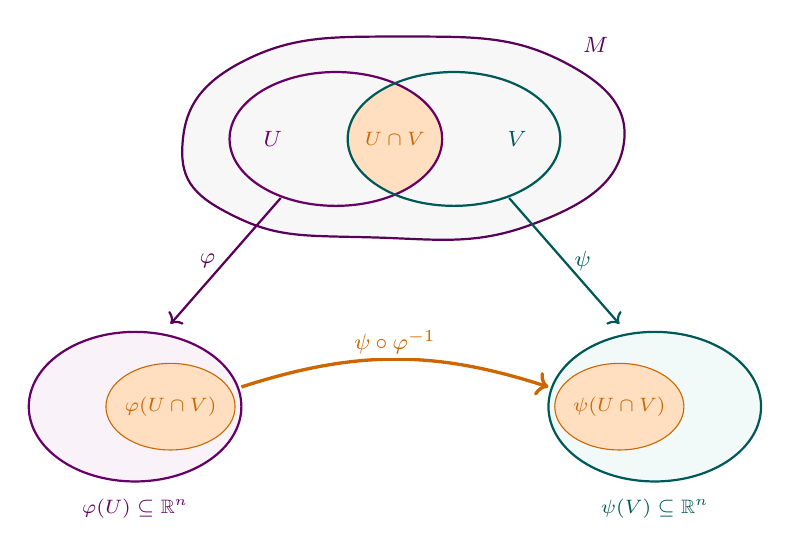
\begin{tikzpicture}
\draw[thick, violet!70!black, fill=gray!6] plot[smooth cycle, tension=0.8] coordinates {(-2.7,3.0) (-1.9,4.1) (0.1,4.4) (2.1,4.1) (2.9,3.0) (1.7,2.0) (-0.3,1.85) (-2.0,2.1)};
\begin{scope} \clip (-0.75,3.1) ellipse (1.35 and 0.85); \fill[orange!25] (0.75,3.1) ellipse (1.35 and 0.85); \end{scope}
\draw[violet!80!black, thick] (-0.75,3.1) ellipse (1.35 and 0.85); \draw[teal!70!black, thick] (0.75,3.1) ellipse (1.35 and 0.85);
\node[violet!80!black, font=\footnotesize] at (-1.55,3.1) {$U$}; \node[teal!70!black, font=\footnotesize] at (1.55,3.1) {$V$}; \node[orange!80!black, font=\scriptsize] at (0,3.1) {$U\cap V$};
\node[violet!70!black, font=\footnotesize] at (2.55,4.3) {$M$};
\draw[violet!80!black, thick, fill=violet!5] (-3.3,-0.3) ellipse (1.35 and 0.95); \fill[orange!25] (-2.85,-0.3) ellipse (0.82 and 0.55); \draw[orange!80!black] (-2.85,-0.3) ellipse (0.82 and 0.55);
\draw[teal!70!black, thick, fill=teal!5] (3.3,-0.3) ellipse (1.35 and 0.95); \fill[orange!25] (2.85,-0.3) ellipse (0.82 and 0.55); \draw[orange!80!black] (2.85,-0.3) ellipse (0.82 and 0.55);
\node[violet!80!black, font=\scriptsize, align=center] at (-3.3,-1.6) {$\varphi(U) \subseteq \mathbb{R}^n$}; \node[teal!70!black, font=\scriptsize, align=center] at (3.3,-1.6) {$\psi(V) \subseteq \mathbb{R}^n$};
\node[orange!80!black, font=\scriptsize] at (-2.85,-0.3) {$\varphi(U\cap V)$}; \node[orange!80!black, font=\scriptsize] at (2.85,-0.3) {$\psi(U\cap V)$};
\draw[->, thick, violet!70!black] (-1.45,2.35) -- node[left, font=\footnotesize] {$\varphi$} (-2.85,0.75);
\draw[->, thick, teal!70!black] (1.45,2.35) -- node[right, font=\footnotesize] {$\psi$} (2.85,0.75);
\draw[->, very thick, orange!80!black] (-1.95,-0.05) to[bend left=18] node[above, font=\footnotesize, fill=white, inner sep=1.5pt] {$\psi\circ\varphi^{-1}$} (1.95,-0.05);
\end{tikzpicture}
\end{center}

Two charts on the same manifold. On the overlap $U \cap V$ (orange) both charts apply, and the two pictures of it, $\varphi(U \cap V)$ and $\psi(U \cap V)$, are compared by the transition map $\psi \circ \varphi^{-1}$ --- a homeomorphism between open subsets of $\mathbb{R}^n$ by Proposition~\ref{prop:transition-homeo}. Chapter~3 defines smooth structures by asking these maps to be smooth.


\begin{rembox}[Preview: What Makes a Manifold \emph{Differentiable}]\label{rem:preview-what-makes-manifold-differentiable}
For a topological manifold, transition functions are homeomorphisms between open subsets of $\mathbb{R}^n$---and that is all one can say. To speak of \emph{differentiable} manifolds, we will \textbf{require} that all transition functions be differentiable (in fact $C^\infty$).

Why is this the right move? Differentiability is not a topological notion: it makes no sense to ask whether a map $X \to \mathbb{R}$ on an abstract topological space is differentiable, because $X$ has no linear structure. What \emph{does} make sense is to pull $f$ back to Euclidean space via a chart, $f \circ \varphi^{-1} : A \to \mathbb{R}$, and ask whether \emph{that} is differentiable. For this to be independent of the chart chosen, one needs $f \circ \psi^{-1} = (f \circ \varphi^{-1}) \circ (\varphi \circ \psi^{-1})$ to be differentiable whenever $f \circ \varphi^{-1}$ is---which is exactly the requirement that transition functions be differentiable. (He expected to begin this on Wednesday; in the event, Lecture 2 stayed with topology---see \ref{sec:new-spaces}.)
\end{rembox}

% ============================================================================
% Lecture 2 (Wed Sep 2, 2026)
% SECTION 4: NEW SPACES FROM OLD
% ============================================================================
\begin{propbox}[Manifolds Are Locally Compact]\thmlabel{prop:locally-compact}
Every topological manifold $M$ is \emph{locally compact}: every point $q \in M$ has an open neighbourhood $V$ whose closure $\overline V$ is compact.
\leeref{Proposition 1.12}
\end{propbox}

\begin{proof}
\textit{(Lecture~14, asking for it to be added to the notes: ``that's obviously true, because you go down to Euclidean space. You have an open set. You just take the ball \ldots\ and pull it up''; filled in.)} Take a chart $(U, \varphi)$ at $q$ and $\varepsilon > 0$ with the closed ball $\overline{B}_\varepsilon(\varphi(q)) \subseteq \varphi(U)$. Put $V = \varphi^{-1}\big(B_\varepsilon(\varphi(q))\big)$, open in $U$ and hence in $M$, and $K = \varphi^{-1}\big(\overline{B}_\varepsilon(\varphi(q))\big)$. $K$ is compact, the image of a compact set under the continuous map $\varphi^{-1}$, hence closed in the Hausdorff space $M$. Since $V \subseteq K$, also $\overline V \subseteq K$, and a closed subset of a compact set is compact.
\end{proof}

% ============================================================================
% Lecture 2 (Wed Sep 2, 2026)
% SECTION 4: NEW SPACES FROM OLD
% ============================================================================
\section{Subspaces and Products}\label{sec:new-spaces}

\roadmark{Thread: quotients}{New spaces from old, first the easy constructions: subspaces and products, with the universal properties that make maps into them easy to check.}

\textit{Reference: Lee Appendix A (``Subspaces, Products, Disjoint Unions, and Quotients''); MATH 590 notes \S5 (subspaces), \S4 (products), \S12 (quotients).}

\begin{rembox}[Why This Section]\label{rem:why-this-section}
Many of the most important manifolds are not defined by charts directly but are \emph{constructed} out of other spaces: complex projective space, Grassmannians, moduli spaces are all quotients. Uribe: ``quotients are the most important construction; a lot of really neat, important manifolds are constructed as quotients of others.'' The guiding question of the lecture, for each construction, is whether the two point-set conditions in the definition of a manifold are \emph{heritable}: if $X$ is $T_2$ and second countable, is the new space too? For subspaces and products the answer is an easy yes; for quotients \emph{everything can go wrong}, and the substance of the lecture is a usable criterion for when it doesn't.
\end{rembox}

\subsection{Subspaces}\label{sub:subspaces}

\begin{defbox}[Subspace Topology]\deflabel{def:subspace}
Let $X$ be a topological space and $S \subseteq X$ a subset. The \textbf{subspace topology} on $S$ is defined by: $V \subseteq S$ is open $\iff$ there exists $U \subseteq X$ open such that $V = U \cap S$.
\leeref{App.~A, \emph{Subspaces, Products, Disjoint Unions, and Quotients}}
\end{defbox}

\begin{rembox}\label{rem:new-spaces}
In 590 \S5 the same topology was defined by naming it as a collection, $\mathcal{T}_S = \{\, U \cap S \mid U \in \mathcal{T} \,\}$; Definition~\ref{def:subspace} just says which sets belong to it. Three facts about it from 590 are used repeatedly in these notes and are recorded here with proofs.
\end{rembox}

\begin{lembox}[Basis of a Subspace]\thmlabel{lem:subspace-basis}
If $\mathcal{B}$ is a basis for $X$ and $S \subseteq X$, then $\mathcal{B}_S = \{\, B \cap S \mid B \in \mathcal{B} \,\}$ is a basis for the subspace topology on $S$.
\leeref{App.~A, \emph{Subspaces, Products, Disjoint Unions, and Quotients}}
\end{lembox}

\begin{proof}
Each $B \cap S$ is open in $S$ by definition. Let $V$ be open in $S$ and $p \in V$; write $V = U \cap S$ with $U$ open in $X$. Since $p \in U$, there is $B \in \mathcal{B}$ with $p \in B \subseteq U$, and then $p \in B \cap S \subseteq U \cap S = V$. This is Definition~\ref{def:basis}.
\end{proof}

\begin{lembox}[Open in Open is Open]\thmlabel{lem:open-in-open}
Let $S \subseteq X$ be open in $X$. If $V \subseteq S$ is open in the subspace topology of $S$, then $V$ is open in $X$.
\leeref{App.~A, \emph{Subspaces, Products, Disjoint Unions, and Quotients}}
\end{lembox}

\begin{proof}
$V = U \cap S$ for some $U$ open in $X$, and $U \cap S$ is an intersection of two open subsets of $X$.
\end{proof}

\begin{propbox}[Universal Property of the Subspace Topology]\thmlabel{prop:univ-subspace}
Let $S \subseteq X$ carry the subspace topology and let $\iota : S \hookrightarrow X$ be the inclusion.
\begin{enumerate}
    \item $\iota$ is continuous, and the subspace topology is the coarsest topology on $S$ for which it is.
    \item For any topological space $Z$ and any function $f : Z \to S$,
    \[
    f \text{ is continuous} \iff \iota \circ f : Z \to X \text{ is continuous.}
    \]
\end{enumerate}
\leeref{Proposition A.17(a)}
\end{propbox}

\begin{proof}
\textit{(Not from lecture; filled in.)} (1) For $U$ open in $X$, $\iota^{-1}(U) = U \cap S$ is open in $S$, so $\iota$ is continuous. If $\mathcal{T}'$ is any topology on $S$ making $\iota$ continuous, then $\mathcal{T}'$ contains $\iota^{-1}(U) = U \cap S$ for every open $U \subseteq X$, i.e.\ $\mathcal{T}'$ contains every open set of the subspace topology.

(2) ($\Rightarrow$) Composition of continuous maps. ($\Leftarrow$) Let $V$ be open in $S$, $V = U \cap S$ with $U$ open in $X$. Since $f$ takes values in $S$,
\[
f^{-1}(V) = f^{-1}(U \cap S) = f^{-1}(U) = \{z \mid f(z) \in U\} = \{z \mid \iota(f(z)) \in U\} = (\iota \circ f)^{-1}(U),
\]
which is open in $Z$.
\end{proof}

\begin{corbox}[The Universal Property Characterizes the Subspace Topology]\thmlabel{cor:univ-subspace-characterizes}
The subspace topology is the unique topology $\mathcal{T}$ on $S$ such that, for every space $Z$, a map $f : Z \to (S, \mathcal{T})$ is continuous if and only if $\iota \circ f : Z \to X$ is continuous.
\leeref{Proposition A.17(b)}
\end{corbox}

\begin{proof}
The subspace topology has the property by Proposition~\ref{prop:univ-subspace}(2). Suppose $\mathcal{T}$ has it. Taking $Z = (S, \mathcal{T})$ and $f = \mathrm{id}$, which is continuous, $\iota$ is continuous for $\mathcal{T}$, so $\mathcal{T}$ contains the subspace topology, the coarsest such (Proposition~\ref{prop:univ-subspace}(1)). Taking $Z$ to be $S$ with the subspace topology and $f = \mathrm{id}$, the composite $\iota \circ \mathrm{id} = \iota$ is continuous, so the property makes $\mathrm{id}$ continuous from the subspace topology to $\mathcal{T}$, i.e.\ $\mathcal{T}$ is contained in the subspace topology.
\end{proof}

This completes the pattern: each of the three constructions --- subspace, product (Corollary~\ref{cor:univ-product-characterizes}) and quotient (Corollary~\ref{cor:univ-characterizes}) --- has its topology characterized by its universal property.

\begin{thmbox}[Subspaces Inherit Both Conditions]\thmlabel{thm:subspace-inherit}
Let $S \subseteq X$ carry the subspace topology.
\begin{enumerate}
    \item If $X$ is $T_2$, then so is $S$.
    \item If $X$ is second countable, then so is $S$.
\end{enumerate}
\leeref{App.~A, \emph{Subspaces, Products, Disjoint Unions, and Quotients}}
\end{thmbox}

\begin{proof}[Proof (only sketched in lecture)]
(1) Let $p \neq q$ in $S$. Since $X$ is $T_2$, there are disjoint open sets $U \ni p$, $V \ni q$ in $X$. Then $U \cap S$ and $V \cap S$ are disjoint neighborhoods of $p$ and $q$ in $S$.

(2) If $\{U_\alpha\}_{\alpha \in A}$ is a countable basis of $X$, then $\{U_\alpha \cap S\}_{\alpha \in A}$ is a basis of $S$ by Lemma~\ref{lem:subspace-basis}, and it is indexed by the same countable set $A$.
\end{proof}

\begin{propbox}[Open Subsets of Manifolds Are Manifolds]\thmlabel{prop:open-submanifold}
An open subset $S$ of a topological $n$-manifold $X$, with the subspace topology, is a topological $n$-manifold.
\leeref{Example 1.26}
\end{propbox}

\begin{proof}
$S$ is Hausdorff and second countable by Theorem~\ref{thm:subspace-inherit}. For $p \in S$ choose a chart $(U, \varphi)$ of $X$ at $p$. Then $U \cap S$ is open in $X$, hence in $S$, and $(U \cap S, \varphi|_{U \cap S})$ is a chart by Lemma~\ref{lem:chart-modify}(1). Proposition~\ref{prop:open-charts} finishes. (Lemma~\ref{lem:open-in-open} is what makes ``open in $S$'' and ``open in $X$'' interchangeable here.)
\end{proof}

\begin{defbox}[Open Submanifold]\deflabel{def:open-submanifold}
An \textbf{open submanifold} of a topological $n$-manifold $X$ is an open subset $S \subseteq X$ with the subspace topology --- a topological $n$-manifold by Proposition~\ref{prop:open-submanifold}.
\leeref{Example 1.26}
\end{defbox}

\begin{rembox}[What Subspaces Do Not Inherit]\label{rem:what-subspaces-do-not-inherit}
Local Euclideanness is \emph{not} hereditary: $\mathbb{R}$ is a $1$-manifold, but its subspace $\mathbb{Q}$ is not locally Euclidean (Example~\ref{ex:fails-loceuc}). By the proposition, openness is exactly what rescues it.
\end{rembox}

\subsection{Products}

\begin{defbox}[Product Topology]\deflabel{def:product-topology}
Let $X, Y$ be topological spaces. The \textbf{product topology} on $X \times Y$ is the one having
\[
\mathcal{B} = \{\, U \times V \mid U \subseteq X \text{ open},\ V \subseteq Y \text{ open} \,\}
\]
as a basis.
\end{defbox}

\begin{propbox}[The Product Basis Generates a Topology]\thmlabel{prop:product-basis}
The collection $\mathcal{B}$ of products $U \times V$ of open sets satisfies the axioms of Definition~\ref{def:basis-alt}, so it is a basis for a topology on $X \times Y$.
\leeref{App.~A, \emph{Subspaces, Products, Disjoint Unions, and Quotients}}
\end{propbox}

\begin{proof}
\textit{(Lecture~2 described the product topology by boxes --- ``for any point $(x,y)$ in $A$, I can fit a box''; that the boxes form a basis is filled in.)} Axiom 1 is clear, since $X \times Y \in \mathcal{B}$. Axiom 2 holds with room to spare, because $\mathcal{B}$ is closed under finite intersections:
\[
(U_1 \times V_1) \cap (U_2 \times V_2) = (U_1 \cap U_2) \times (V_1 \cap V_2). \qedhere
\]
\end{proof}

\begin{propbox}[Box Characterization of Open Sets]\thmlabel{prop:box}
$A \subseteq X \times Y$ is open in the product topology if and only if
\[
\forall\, (x, y) \in A\ \ \exists \text{ neighborhoods } U \text{ of } x \text{ in } X \text{ and } V \text{ of } y \text{ in } Y \text{ such that } U \times V \subseteq A.
\]
\leeref{App.~A, \emph{Subspaces, Products, Disjoint Unions, and Quotients}}
\end{propbox}

\begin{center}
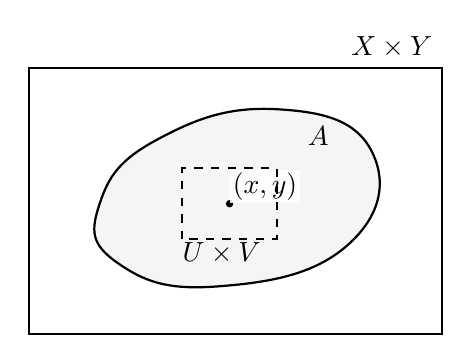
\begin{tikzpicture}[scale=0.75]
    \draw[thick] (0,0) rectangle (7,4.5);
    \node[anchor=south east] at (7,4.5) {$X \times Y$};
    \draw[thick, fill=gray!8] plot [smooth cycle, tension=0.8] coordinates {(1.5,1.2) (3.2,0.8) (5.4,1.5) (5.8,3.1) (4.2,3.8) (2.2,3.3) (1.2,2.2)};
    \node at (4.9,3.35) {$A$};
    \filldraw (3.4,2.2) circle (1.5pt) node[anchor=south west, inner sep=1pt, fill=white, fill opacity=0.85, text opacity=1, ] {$(x,y)$};
    \draw[dashed, thick] (2.6,1.6) rectangle (4.2,2.8);
    \node[anchor=north west, inner sep=1pt] at (2.55,1.6) {$U \times V$};
\end{tikzpicture}
\end{center}

\begin{proof}
If $A$ is open and $(x,y) \in A$, then by Definition~\ref{def:basis} applied to the basis $\mathcal{B}$ there is a basis element $U \times V$ with $(x,y) \in U \times V \subseteq A$; that is the box. Conversely, if every point of $A$ admits such a box, then $A$ is a union of basis elements, hence open (Proposition~\ref{prop:basis-equiv}).
\end{proof}

\begin{rembox}[Cartoons]\label{rem:cartoons}
Uribe on the figure above: diagrams of this kind are ``incredibly important and useful''---an open set in a product is one in which every point can be surrounded by a \emph{box}. The box picture is what actually gets used in proofs (it reappears in the second-countability part of Theorem~\ref{thm:product-inherit} and in the proof of the Hausdorff Criterion below), and he encourages drawing it every time.
\end{rembox}

\begin{propbox}[Coarsest Topology with Continuous Projections]\thmlabel{prop:product-coarsest}
Let $\pi_X : X \times Y \to X$ and $\pi_Y : X \times Y \to Y$ be the projection maps. The product topology is the \emph{coarsest} topology on $X \times Y$ for which $\pi_X$ and $\pi_Y$ are both continuous.
\leeref{App.~A, \emph{Subspaces, Products, Disjoint Unions, and Quotients}}
\end{propbox}

\begin{proof}[Proof (not given in lecture)]
The product topology makes the projections continuous: $\pi_X^{-1}(U) = U \times Y$ and $\pi_Y^{-1}(V) = X \times V$ are basis elements. Conversely, let $\mathcal{T}$ be any topology on $X \times Y$ making both projections continuous. For $U \subseteq X$, $V \subseteq Y$ open, $\mathcal{T}$ contains $U \times Y$ and $X \times V$, hence their intersection $U \times V$. So $\mathcal{T}$ contains the basis $\mathcal{B}$, hence contains all unions of members of $\mathcal{B}$, i.e.\ every set open in the product topology. Thus the product topology is contained in every such $\mathcal{T}$.
\end{proof}

\begin{thmbox}[Universal Property of the Product]\thmlabel{thm:univ-product}
Let $Z$ be any topological space and $F : Z \to X \times Y$ a function. Then
\[
F \text{ is continuous} \iff \text{both } \pi_X \circ F \text{ and } \pi_Y \circ F \text{ are continuous.}
\]
\leeref{Proposition A.23(a)}
\end{thmbox}

\begin{proof}[Proof (one direction in lecture; other filled in)]
($\Rightarrow$) The projections are continuous, and compositions of continuous maps are continuous.

($\Leftarrow$) It suffices to check that preimages of \emph{basis} elements are open (a preimage of a union is the union of the preimages). For $U \times V \in \mathcal{B}$,
\[
F^{-1}(U \times V) = \{z \mid \pi_X(F(z)) \in U \text{ and } \pi_Y(F(z)) \in V\} = (\pi_X \circ F)^{-1}(U) \cap (\pi_Y \circ F)^{-1}(V),
\]
an intersection of two open sets.
\end{proof}

\begin{rembox}[Why the Universal Property Matters]\label{rem:why-universal-property-matters}
``To check that $F$ is continuous, you just check component by component.'' Uribe flagged that the same pattern will reappear for \emph{differentiability}: a map into a product of manifolds will be smooth iff its components are. In Lee's language this is the \emph{characteristic property} of the product topology (Lee Prop.\ A.16), and it characterizes the product topology uniquely (Corollary~\ref{cor:univ-product-characterizes} below). Together with the previous proposition this gives two independent abstract descriptions of the same topology---``coarsest making projections continuous'' and ``the one that lets you check maps componentwise.''

Compare Proposition~\ref{prop:univ-subspace}: the subspace topology is the coarsest making the inclusion continuous, and continuity of a map \emph{into} $S$ is checked by composing with $\iota$. The quotient topology will complete the pattern in the opposite direction (Proposition~\ref{prop:univ-quotient}): it is the \emph{finest} making $\pi$ continuous, and continuity of a map \emph{out of} $X/{\sim}$ is checked by precomposing with $\pi$.
\end{rembox}

\begin{corbox}[The Universal Property Characterizes the Product Topology]\thmlabel{cor:univ-product-characterizes}
The product topology is the unique topology $\mathcal{T}$ on $X \times Y$ such that, for every space $Z$, a map $f : Z \to (X \times Y, \mathcal{T})$ is continuous if and only if $\pi_X \circ f$ and $\pi_Y \circ f$ are continuous.
\leeref{Proposition A.23(b)}
\end{corbox}

\begin{proof}
The product topology has the property by Theorem~\ref{thm:univ-product}. Suppose $\mathcal{T}$ has it. Taking $Z = (X \times Y, \mathcal{T})$ and $f = \mathrm{id}$, which is continuous, the projections are continuous for $\mathcal{T}$, so $\mathcal{T}$ contains the product topology by Proposition~\ref{prop:product-coarsest}. Taking $Z$ to be $X \times Y$ with the product topology and $f = \mathrm{id}$, whose components $\pi_X$ and $\pi_Y$ are continuous there, the property makes $\mathrm{id}$ continuous from the product topology to $\mathcal{T}$, i.e.\ $\mathcal{T}$ is contained in the product topology.
\end{proof}

\begin{thmbox}[Products Inherit Both Conditions]\thmlabel{thm:product-inherit}
\begin{enumerate}
    \item If $X$ and $Y$ are both $T_2$, then $X \times Y$ is $T_2$.
    \item If $X$ and $Y$ are both second countable, then $X \times Y$ is second countable.
\end{enumerate}
\leeref{Example 1.8}
\end{thmbox}

\begin{proof}[Proof (not given in lecture --- ``it's point-set topology'')]
(1) Let $(x, y) \neq (x', y')$; they differ in some coordinate, say $x \neq x'$ (the other case is symmetric). Choose disjoint open $U \ni x$, $U' \ni x'$ in $X$. Then $U \times Y$ and $U' \times Y$ are disjoint open neighborhoods of the two points.

(2) If $\{U_\alpha\}_{\alpha \in A}$ and $\{V_\beta\}_{\beta \in B}$ are countable bases of $X$ and $Y$, then $\{U_\alpha \times V_\beta\}_{(\alpha,\beta) \in A \times B}$ is a countable collection ($A \times B$ countable), and it is a basis: given $(x,y) \in W$ open, the box characterization gives $U \times V \subseteq W$ around $(x,y)$, and then $U_\alpha \subseteq U$, $V_\beta \subseteq V$ around $x, y$ give $(x,y) \in U_\alpha \times V_\beta \subseteq W$.
\end{proof}

\begin{rembox}\label{rem:new-spaces-2}
Both statements extend to finite products by induction. For \emph{infinite} products the story is subtler (product vs.\ box topology, 590 \S10), but finite products are all we need: they are how product manifolds like the torus $T^n = S^1 \times \cdots \times S^1$ will get their point-set hygiene for free, leaving only local Euclideanness to check.
\end{rembox}

% ============================================================================
% SECTION: QUOTIENT SPACES AND OPEN MAPS
% ============================================================================

\section{Quotient Spaces and Open Maps}\label{sec:quotient-spaces}\label{sub:quotients}

\roadmark{Thread: quotients}{Manifolds built by gluing and identifying points. The quotient topology, and open maps and open relations --- the tool that keeps quotients second countable.}

\begin{defbox}[Quotient Space and Quotient Topology]\deflabel{def:quotient}
Let $X$ be a topological space and $\sim$ an equivalence relation on $X$. Form the \textbf{quotient space}
\[
X/{\sim} \;=\; \{\, [x] \mid x \in X \,\}, \qquad [x] = \{y \in X \mid y \sim x\},
\]
the set of equivalence classes, with the natural surjection $\pi : X \to X/{\sim}$, $x \mapsto [x]$. The \textbf{quotient topology} on $X/{\sim}$ is defined by:
\[
W \subseteq X/{\sim} \text{ is open} \iff \pi^{-1}(W) \subseteq X \text{ is open in } X.
\]
\leeref{App.~A, \emph{Subspaces, Products, Disjoint Unions, and Quotients}}
\end{defbox}

\begin{propbox}[The Quotient Topology Is the Finest Making $\pi$ Continuous]\thmlabel{prop:quotient-finest}
The projection $\pi : X \to X/{\sim}$ is continuous, and the quotient topology is the \emph{finest} topology on $X/{\sim}$ with this property: every topology $\mathcal{T}'$ on $X/{\sim}$ for which $\pi$ is continuous is contained in it.
\leeref{App.~A, \emph{Subspaces, Products, Disjoint Unions, and Quotients}}
\end{propbox}

\begin{proof}
\textit{(Not from lecture; filled in.)} If $W$ is open in $X/{\sim}$ then $\pi^{-1}(W)$ is open in $X$ by definition, so $\pi$ is continuous. If $\pi$ is continuous for $\mathcal{T}'$, then every $W \in \mathcal{T}'$ has $\pi^{-1}(W)$ open in $X$, hence $W$ is open in the quotient topology.
\end{proof}


\begin{rembox}[How to Read a Quotient]\label{rem:how-read-quotient}
A quotient space is easy to define and easy to lose track of. Whenever a quotient $X/{\sim}$ appears in these notes, four things are made explicit, and it is worth demanding them of every quotient you meet:
\begin{enumerate}
    \item \textbf{What a point is.} A point of $X/{\sim}$ is an equivalence class $[x]$, i.e.\ a \emph{subset} of $X$. Say which subset.
    \item \textbf{What $\pi$ does.} $\pi(x) = [x]$: it sends a point of $X$ to the class containing it.
    \item \textbf{What the open sets are.} $W \subseteq X/{\sim}$ is open iff $\pi^{-1}(W) = \bigcup_{[x] \in W} [x]$---the union in $X$ of all the classes belonging to $W$---is open in $X$. So the open sets of $X/{\sim}$ correspond exactly to the open subsets of $X$ that are \emph{unions of classes} (the \emph{saturated} open sets, \S\ref{sub:open-relations}).
    \item \textbf{What an identification does.} When $X/{\sim}$ is identified with a concrete space $Y$ via a bijection $\Phi$, say what $\Phi$ does to a class, and what its inverse does to a point of $Y$.
\end{enumerate}
For the line with two origins (Example~\ref{ex:two-origins-quotient}): a point is a pair $\{(x,1), (x,2)\}$ for $x \neq 0$ or a singleton $\{(0,i)\}$; $\pi$ forgets the label except at $0$; a set is open iff its preimage, a union of such pairs and singletons, is open in the two lines; the identification with Example~\ref{ex:two-origins} sends $\{(x,1),(x,2)\} \mapsto x$ and $\{(0,i)\} \mapsto 0_i$.
\end{rembox}

\begin{rembox}[Warning: Nothing Is Automatically Inherited]\label{rem:warning-nothing-automatically-inherited}
\textbf{Neither $T_2$ nor second countability of $X$ is automatically inherited by $X/{\sim}$.} This is the reason the lecture spends most of its time here: the constructions that produce interesting manifolds are quotients, so we need theorems telling us \emph{when} the quotient is $T_2$ (and second countable) --- these properties must be earned, not assumed.
\end{rembox}

\begin{exbox}[Failure of Hausdorffness --- the Line with Two Origins as a Quotient]\exlabel{ex:two-origins-quotient}
Let
\[
X = (\mathbb{R} \times \{1\}) \cup (\mathbb{R} \times \{2\})
\]
(two disjoint copies of the real line), and define $(x, 1) \sim (x, 2)$ for all $x \neq 0$ --- these, together with the relations forced by reflexivity and symmetry, are the only identifications. In particular $(0,1) \not\sim (0,2)$: the two origins survive as distinct points. The quotient space is exactly the real line with two origins of Example~\ref{ex:two-origins}, which is not $T_2$ --- even though $X$ itself, a disjoint union of two lines, is a metrizable space with every good property one could ask for.
\leeref{Problem 1-1}
\end{exbox}

\begin{propbox}[The Two Constructions Agree]\thmlabel{prop:two-origins-agree}
The bijection sending the class $\{(x,1),(x,2)\}$ to $x$ for $x \neq 0$ and the class $\{(0,i)\}$ to $0_i$ is a homeomorphism from $X/{\sim}$, with the quotient topology, onto the line with two origins of Example~\ref{ex:two-origins}, with the topology generated by the neighborhood bases $(-\varepsilon,0) \cup \{0_i\} \cup (0,\varepsilon)$.
\end{propbox}

\begin{proof}[Exercise]
Set up the bijection as above and check that a subset downstairs is open for one topology iff it is open for the other; by Proposition~\ref{prop:GH-open-sets}-style reasoning it is enough to compare the two on the basic sets of Example~\ref{ex:two-origins}, pulling each back along $\pi$. Assigned in lecture and left here.
\end{proof}

The single most useful fact about the quotient topology --- that a map \emph{out} of a quotient is continuous as soon as its composite with $\pi$ is, and that a map on $X$ constant on the classes descends to one on $X/{\sim}$ --- is Theorem~\ref{thm:univ-quotient-full} below. It is stated in \S\ref{sub:quotient-maps} because its natural generality is quotient maps rather than quotient spaces.

\subsection{Open Maps and Open Relations}\label{sub:open-relations}

\begin{defbox}[Open Map]\deflabel{def:open-map}
A continuous map $F : X \to Y$ between topological spaces is \textbf{open} if for every open $U \subseteq X$, the image $F(U)$ is open in $Y$.
\end{defbox}

\begin{exbox}[Projections Are Open]\exlabel{ex:proj-open}
$\pi_X : X \times Y \to X$ is always an open map.
\end{exbox}

\begin{proof}[Proof (not given in lecture --- ``go home and check yourself'')]
First, for a basis element: $\pi_X(U \times V) = U$ if $V \neq \emptyset$ (and $= \emptyset$ if $V = \emptyset$), open either way. A general open $A \subseteq X \times Y$ is a union of basis elements, $A = \bigcup_i U_i \times V_i$, and images commute with unions:
\[
\pi_X(A) = \bigcup_i \pi_X(U_i \times V_i),
\]
a union of open sets.
\end{proof}

\begin{defbox}[Open Equivalence Relation]\deflabel{def:open-equivalence-relation}
An equivalence relation $\sim$ on $X$ is \textbf{open} if the projection $\pi : X \to X/{\sim}$ is an open map.
\end{defbox}

\begin{exbox}[Non-Example]\exlabel{ex:nonopen-relation}
Let $X = \mathbb{R}$ and let $\sim$ be the equivalence relation generated by the single non-trivial identification $0 \sim 1$ (glue the two points; the quotient looks like a line with a small loop). Take the open set $\left(-\tfrac12, \tfrac12\right)$ and compute the preimage of its image:
\[
\pi^{-1}\!\left(\pi\!\left(-\tfrac12, \tfrac12\right)\right) = \left(-\tfrac12, \tfrac12\right) \cup \{1\},
\]
because the identified point $[0] = [1]$ has the \emph{two} preimages $0$ and $1$. This set is not open in $\mathbb{R}$ (no neighborhood of $1$ fits inside), so $\pi\left(-\tfrac12,\tfrac12\right)$ is not open in the quotient, and $\sim$ is not an open relation. Uribe: ``I love little examples like this.''
\end{exbox}

\begin{defbox}[Saturation and Saturated Sets]\deflabel{def:saturation}
Let $\sim$ be an equivalence relation on a set $X$ with quotient map $\pi : X \to X/{\sim}$. For any subset $U \subseteq X$, the \textbf{saturation} of $U$ is
\[
\tilde U \;:=\; \pi^{-1}(\pi(U)) \;=\; \{\, y \in X \mid \exists\, x \in U \text{ such that } y \sim x \,\} \;=\; \bigcup_{x \in U} [x],
\]
the union of all equivalence classes that meet $U$. A subset $S \subseteq X$ is \textbf{saturated} if $S = \tilde S$; equivalently, $S$ is a union of equivalence classes; equivalently, $S = \pi^{-1}(W)$ for some $W \subseteq X/{\sim}$ (namely $W = \pi(S)$).
\end{defbox}

\begin{center}
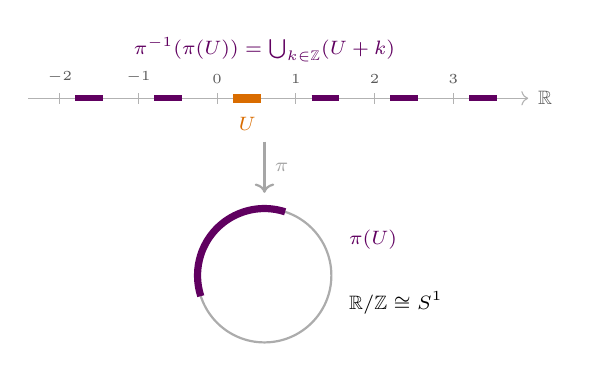
\begin{tikzpicture}
\draw[->, gray!60] (-2.4,0) -- (3.95,0) node[right, font=\scriptsize, text=gray!70!black] {$\mathbb{R}$};
\draw[gray!60] (-2,-0.07) -- (-2,0.07) node[above, font=\tiny, text=gray!70!black] {$-2$};
\draw[gray!60] (-1,-0.07) -- (-1,0.07) node[above, font=\tiny, text=gray!70!black] {$-1$};
\draw[gray!60] (0,-0.07) -- (0,0.07) node[above, font=\tiny, text=gray!70!black] {$0$};
\draw[gray!60] (1,-0.07) -- (1,0.07) node[above, font=\tiny, text=gray!70!black] {$1$};
\draw[gray!60] (2,-0.07) -- (2,0.07) node[above, font=\tiny, text=gray!70!black] {$2$};
\draw[gray!60] (3,-0.07) -- (3,0.07) node[above, font=\tiny, text=gray!70!black] {$3$};
\draw[violet!75!black, line width=2.2pt] (-1.80,0) -- (-1.45,0);
\draw[violet!75!black, line width=2.2pt] (-0.80,0) -- (-0.45,0);
\draw[violet!75!black, line width=2.2pt] (0.20,0) -- (0.55,0);
\draw[violet!75!black, line width=2.2pt] (1.20,0) -- (1.55,0);
\draw[violet!75!black, line width=2.2pt] (2.20,0) -- (2.55,0);
\draw[violet!75!black, line width=2.2pt] (3.20,0) -- (3.55,0);
\draw[orange!85!black, line width=3.2pt] (0.20,0) -- (0.55,0); \node[orange!85!black, font=\scriptsize] at (0.38,-0.32) {$U$};
\node[violet!75!black, font=\scriptsize] at (0.6,0.62) {$\pi^{-1}(\pi(U)) = \bigcup_{k\in\mathbb{Z}} (U + k)$};
\draw[->, thick, gray!70] (0.6,-0.55) -- node[right, font=\scriptsize] {$\pi$} (0.6,-1.2);
\draw[thick, gray!65] (0.60,-2.25) circle (0.85);
\draw[violet!75!black, line width=2.6pt] (0.60,-2.25) ++(72.0:0.85) arc (72.0:198.0:0.85);
\node[violet!75!black, font=\scriptsize, anchor=west] at (1.55,-1.80) {$\pi(U)$};
\node[font=\scriptsize, anchor=west] at (1.55,-2.60) {$\mathbb{R}/\mathbb{Z} \cong S^1$};
\end{tikzpicture}
\end{center}

Saturation for the relation $x \sim y \iff x - y \in \mathbb{Z}$ on $\mathbb{R}$, whose quotient is the circle (Example~\ref{ex:circle-RZ}). The saturation of the interval $U$ is the union of all its integer translates, $\pi^{-1}(\pi(U))$: everything the quotient map cannot tell apart from $U$. It is open because each translate is --- the mechanism behind ``orbit relations are open'' (Lemma~\ref{lem:orbit-open}) --- and its image $\pi(U)$ is an open arc of the circle.

\begin{lembox}[Basic Properties of Saturation]\thmlabel{lem:saturation}
For all $U, V \subseteq X$ and any family $(U_\alpha)$ of subsets:
\begin{enumerate}
    \item $U \subseteq \tilde U$, and $\tilde{\tilde U} = \tilde U$ (the saturation is saturated).
    \item $U \subseteq V \Rightarrow \tilde U \subseteq \tilde V$, and $\widetilde{\bigcup_\alpha U_\alpha} = \bigcup_\alpha \tilde U_\alpha$.
    \item $\pi(\tilde U) = \pi(U)$.
    \item The three descriptions of ``saturated'' in Definition~\ref{def:saturation} are equivalent, and for saturated $S$ one has $\pi^{-1}(\pi(S)) = S$.
\end{enumerate}
\end{lembox}

\begin{proof}
Write $\tilde U = \bigcup_{x \in U}[x]$. (1) $x \in [x]$ gives $U \subseteq \tilde U$. If $y \in \tilde{\tilde U}$ then $y \sim z$ for some $z \in \tilde U$, so $z \sim x$ for some $x \in U$, and transitivity gives $y \sim x$, i.e.\ $y \in \tilde U$; with $\tilde U \subseteq \tilde{\tilde U}$ from the first part, equality follows. (2) Both are immediate from $\tilde U = \bigcup_{x \in U}[x]$: enlarging $U$ enlarges the union, and the union over $\bigcup_\alpha U_\alpha$ is the union of the unions. (3) $\pi(\tilde U) \supseteq \pi(U)$ by (1); conversely $\pi(y)$ for $y \in [x]$, $x \in U$, equals $\pi(x) \in \pi(U)$. (4) If $S = \tilde S$ then $S$ is the union of the classes $[x]$, $x \in S$. If $S$ is a union of classes, $S = \bigcup_{[x] \in W}[x]$ for $W = \pi(S)$, then $\pi^{-1}(W) = \{y \mid [y] \in W\} = S$. If $S = \pi^{-1}(W)$ then $\tilde S = \pi^{-1}(\pi(\pi^{-1}(W))) = \pi^{-1}(W) = S$, using $\pi(\pi^{-1}(W)) = W$ (surjectivity of $\pi$).
\end{proof}

\begin{propbox}[The Saturation Correspondence]\thmlabel{prop:saturation-correspondence}
Let $\pi : X \to X/{\sim}$ be the projection. Then $W \mapsto \pi^{-1}(W)$ is a bijection from the subsets of $X/{\sim}$ onto the saturated subsets of $X$, with inverse $S \mapsto \pi(S)$, and it preserves unions, intersections and complements. Under it, the open subsets of $X/{\sim}$ correspond exactly to the saturated open subsets of $X$, and the closed subsets to the saturated closed subsets.
\leeref{Theorem A.27(c)}
\end{propbox}

\begin{proof}
\textit{(Lecture~2 defined the saturation and stated that a relation is open exactly when saturations of open sets are open; the proof is filled in.)} Every $\pi^{-1}(W)$ is saturated, and $\pi(\pi^{-1}(W)) = W$ because $\pi$ is surjective. Conversely, a saturated $S$ satisfies $\pi^{-1}(\pi(S)) = S$ by Lemma~\ref{lem:saturation}(4). So the two maps are mutually inverse. Taking preimages commutes with unions, intersections and complements. The open sets of $X/{\sim}$ are by definition those $W$ with $\pi^{-1}(W)$ open, which gives the statement for open sets. For closed sets pass to complements, using that the complement of a saturated set is saturated (it is the union of the remaining classes).
\end{proof}

\begin{propbox}[Openness via Saturations]\thmlabel{prop:saturation}
$\sim$ is open $\iff$ for every open $U \subseteq X$, the saturation $\tilde U = \pi^{-1}(\pi(U))$ is open in $X$.
\end{propbox}

\begin{proof}
$\pi$ is open iff $\pi(U)$ is open in $X/{\sim}$ for every open $U \subseteq X$; and by the definition of the quotient topology, $\pi(U)$ is open in $X/{\sim}$ iff $\pi^{-1}(\pi(U)) = \tilde U$ is open in $X$.
\end{proof}

In lecture, saturation was named after the proposition, as the set $\pi^{-1}(\pi(U))$ appearing in it; the notion is worth having on its own (it recurs for orbit spaces in \ref{sec:actions}), which is why it is defined first here, with its elementary properties.

\begin{rembox}[In Words]\label{rem:words}
The saturation of $U$ is $U$ together with everything equivalent to something in $U$ --- ``you push forward and then take the preimage.'' Proposition~\ref{prop:saturation} then reads as a slogan: \emph{$\sim$ is open iff the saturation of every open set is open.} In the non-example above, saturating $\left(-\tfrac12,\tfrac12\right)$ adjoined the isolated point $1$ and destroyed openness. In the $\mathbb{CP}^n$ example below, saturating an open set means rotating it in every possible way, which \emph{preserves} openness --- that contrast is the whole point of the definition.
\end{rembox}

\begin{exbox}[Failure of Second Countability]\exlabel{ex:not-2c-quotient}
Let $X = \mathbb{R}/{\sim}$ with the quotient topology, where $x \sim y$ iff $x = y$ or both $x, y \in \mathbb{Z}$: all integers are collapsed to a single point $x_0$, and $X$ looks like $x_0$ with countably many loops attached. Then $\mathbb{R}$ is second countable but $X$ is not, because $X$ is not first countable at $x_0$.
\end{exbox}
\begin{center}
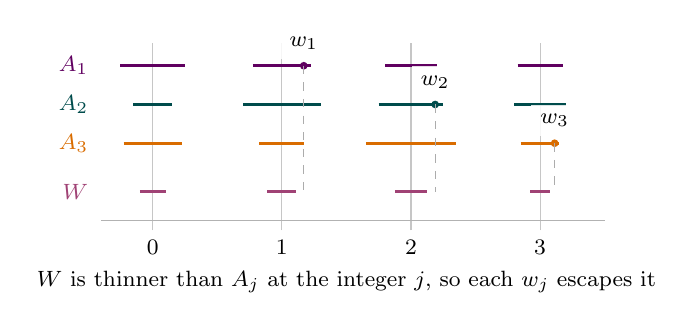
\begin{tikzpicture}[scale=0.82]
\foreach \x in {0,2,4,6} { \draw[gray!45] (\x,-0.15) -- (\x,2.75); }
\draw[gray!60] (-0.8,0) -- (7,0);
\foreach \x/\l in {0/0,2/1,4/2,6/3} { \node[font=\footnotesize,below] at (\x,-0.15) {$\l$}; }
\foreach \i/\a in {0/0.5,2/0.45,4/0.4,6/0.35} { \draw[violet!75!black,very thick] (\i-\a,2.4) -- (\i+\a,2.4); }
\foreach \i/\a in {0/0.3,2/0.6,4/0.5,6/0.4} { \draw[teal!60!black,very thick] (\i-\a,1.8) -- (\i+\a,1.8); }
\foreach \i/\a in {0/0.45,2/0.35,4/0.7,6/0.3} { \draw[orange!85!black,very thick] (\i-\a,1.2) -- (\i+\a,1.2); }
\foreach \i/\a in {0/0.2,2/0.225,4/0.25,6/0.15} { \draw[magenta!60!black,very thick] (\i-\a,0.45) -- (\i+\a,0.45); }
\node[violet!75!black,font=\footnotesize,anchor=east] at (-0.85,2.4) {$A_1$};
\node[teal!60!black,font=\footnotesize,anchor=east] at (-0.85,1.8) {$A_2$};
\node[orange!85!black,font=\footnotesize,anchor=east] at (-0.85,1.2) {$A_3$};
\node[magenta!60!black,font=\footnotesize,anchor=east] at (-0.85,0.45) {$W$};
\fill[violet!75!black] (2.34,2.4) circle (1.7pt);
\fill[teal!60!black] (4.375,1.8) circle (1.7pt);
\fill[orange!85!black] (6.225,1.2) circle (1.7pt);
\draw[dashed,gray!65] (2.34,2.4) -- (2.34,0.45);
\draw[dashed,gray!65] (4.375,1.8) -- (4.375,0.45);
\draw[dashed,gray!65] (6.225,1.2) -- (6.225,0.45);
\node[fill=white, fill opacity=0.85, text opacity=1, font=\footnotesize,anchor=south] at (2.34,2.5) {$w_1$};
\node[fill=white, fill opacity=0.85, text opacity=1, font=\footnotesize,anchor=south] at (4.375,1.9) {$w_2$};
\node[fill=white, fill opacity=0.85, text opacity=1, font=\footnotesize,anchor=south] at (6.225,1.3) {$w_3$};
\node[font=\footnotesize] at (3,-0.95) {$W$ is thinner than $A_j$ at the integer $j$, so each $w_j$ escapes it};
\end{tikzpicture}
\end{center}


\begin{proof}[Proof (PSet 1, Problem 4)]
Write $\pi : \mathbb{R} \to X$, so $\pi^{-1}(x_0) = \mathbb{Z}$ and $\pi^{-1}(\pi(x)) = \{x\}$ for $x \notin \mathbb{Z}$. Two preliminary facts. (i) If $V \subseteq X$ is a neighborhood of $x_0$, then $\pi^{-1}(V)$ is open in $\mathbb{R}$ and contains $\mathbb{Z}$. (ii) If $U \subseteq \mathbb{R}$ is open with $\mathbb{Z} \subseteq U$, then $U$ is saturated---each class is either $\mathbb{Z} \subseteq U$ or a singleton $\{x\} \subseteq U$---so $\pi^{-1}(\pi(U)) = U$ and $\pi(U)$ is a neighborhood of $x_0$ (Definition~\ref{def:saturation} and Lemma~\ref{lem:saturation}(4)).

Suppose $X$ were first countable at $x_0$, with $\{\widetilde U_j\}_{j \in \mathbb{N}}$ a countable basis of neighborhoods of $x_0$, and set $U_j = \pi^{-1}(\widetilde U_j)$, open with $\mathbb{Z} \subseteq U_j$ by (i). For each $j \in \mathbb{N}$ and $n \in \mathbb{Z}$, openness gives a radius $a_{j,n} \in (0, \tfrac14]$ with $(n - a_{j,n}, n + a_{j,n}) \subseteq U_j$; write $A_j = \bigcup_{n \in \mathbb{Z}} (n - a_{j,n}, n + a_{j,n}) \subseteq U_j$. (Radii are capped at $\tfrac14$ so that arms around distinct integers are disjoint: two of them reach out at most $\tfrac12 < 1$.)

\emph{The diagonal neighborhood.} Put
\[
b_n = \begin{cases} a_{n,n}/2, & n \in \mathbb{N}, \\ 1/8, & n \in \mathbb{Z} \setminus \mathbb{N}, \end{cases}
\qquad W = \bigcup_{n \in \mathbb{Z}} (n - b_n,\, n + b_n).
\]
Then $W$ is open, $\mathbb{Z} \subseteq W$, and $b_n \le \tfrac18$ for all $n$.

\emph{No $U_j$ is contained in $W$.} Fix $j \in \mathbb{N}$ and set $w_j = j + \tfrac34 a_{j,j}$. Then $w_j \in A_j \subseteq U_j$, since $|w_j - j| = \tfrac34 a_{j,j} < a_{j,j}$. But $w_j \notin W$: it is not in the arm at $j$, because $j + b_j = j + \tfrac12 a_{j,j} < w_j$; and it is in no other arm, since $|w_j - j| \le \tfrac34 \cdot \tfrac14 < \tfrac14$ while a point of the arm at $m$ is within $b_m \le \tfrac18$ of $m$, so $w_j$ in that arm would force $|j - m| < \tfrac14 + \tfrac18 < 1$, impossible for distinct integers.

\emph{Conclusion.} By (ii), $\widetilde W = \pi(W)$ is a neighborhood of $x_0$. If $\widetilde U_j \subseteq \widetilde W$ for some $j$, taking preimages would give $U_j \subseteq \pi^{-1}(\widetilde W) = W$, contradicting the previous paragraph. So no member of the family sits inside $\widetilde W$, and $\{\widetilde U_j\}$ is not a basis of neighborhoods of $x_0$---a contradiction. Hence $X$ is not first countable at $x_0$, and by Proposition~\ref{prop:2c-implies-1c} it is not second countable.
\end{proof}

\begin{rembox}[Why the Diagonal]\label{rem:why-diagonal}
The mechanism is Cantor's: each candidate $U_j$ is pinned down at the single integer $j$, and $W$ is built to be strictly thinner than $U_j$ exactly there. No countable family can control all of the infinitely many arms at once, because a neighborhood of $x_0$ must specify a radius at \emph{every} integer simultaneously---that is what collapsing infinitely many points to one costs. Theorem~\ref{thm:2c-quotient} is not contradicted, because its hypothesis fails: this relation is \emph{not} open. The saturation of the open set $(-\tfrac12, \tfrac12)$, which meets $\mathbb{Z}$ at $0$, is $(-\tfrac12,\tfrac12) \cup \mathbb{Z}$, and that is not open---no neighborhood of the point $1$ is contained in it.
\end{rembox}

% ============================================================================
% SECTION: QUOTIENT MAPS
% ============================================================================

\section{Quotient Maps}\label{sec:quotient-maps}\label{sub:quotient-maps}

\roadmark{Thread: quotients}{The quotient topology as a property of a map: how quotients are recognized in practice, and how maps out of them are built.}

So far ``quotient'' has named a topology on a set of equivalence classes. The same notion can be phrased as a property of a map, which is often how it is recognized in practice.

\begin{defbox}[Quotient Map]\deflabel{def:quotient-map}
A map $F : X \to Y$ between topological spaces is a \textbf{quotient map} if it is surjective and
\[
U \subseteq Y \text{ is open} \iff F^{-1}(U) \subseteq X \text{ is open}.
\]
\leeref{App.~A, \emph{Subspaces, Products, Disjoint Unions, and Quotients}}
\end{defbox}

\begin{exbox}[Projections onto Quotient Spaces Are Quotient Maps]\exlabel{ex:projection-quotient-map}
The projection $\pi : X \to X/{\sim}$ of Definition~\ref{def:quotient} is a quotient map in the sense of Definition~\ref{def:quotient-map}: it is surjective, and $W$ is open in $X/{\sim}$ if and only if $\pi^{-1}(W)$ is open in $X$, which is the definition of the quotient topology. The next proposition says that these are the only examples.
\end{exbox}

\begin{defbox}[Maps Constant on Fibres]\deflabel{def:constant-fibres}
Let $p : X \to Y$ be a map. A map $g : X \to Z$ is \textbf{constant on the fibres of $p$} if it is constant on $p^{-1}(\{y\})$ for every $y \in Y$; equivalently, $p(x) = p(x')$ implies $g(x) = g(x')$.
\end{defbox}

\begin{thmbox}[Universal Property of a Quotient Map]\thmlabel{thm:univ-quotient-full}
Let $p : X \to Y$ be a quotient map (Definition~\ref{def:quotient-map}), let $Z$ be a topological space, and let $g : X \to Z$ be a map that is constant on the fibres of $p$ (Definition~\ref{def:constant-fibres}). Then there is a \emph{unique} map $f : Y \to Z$ with
\[
f \circ p = g .
\]
Moreover:
\begin{enumerate}
    \item $f$ is continuous $\iff$ $g$ is continuous;
    \item $f$ is a quotient map $\iff$ $g$ is a quotient map.
\end{enumerate}
\leeref{Theorems A.27(a) and A.30}
\end{thmbox}

\begin{center}
\begin{tikzcd}[row sep=3.0em, column sep=3.6em]
X \arrow[r, "g"] \arrow[d, "p"'] & Z \\
Y \arrow[ur, dashed, "f"'] &
\end{tikzcd}
\end{center}

\begin{proof}
\emph{Existence and uniqueness of $f$.} Let $y \in Y$. Since $p$ is surjective the fibre $p^{-1}(\{y\})$ is nonempty; choose $x$ in it and set $f(y) := g(x)$. This does not depend on the choice, because $g$ is constant on that fibre. By construction $f(p(x)) = g(x)$ for every $x \in X$, i.e.\ $f \circ p = g$. If $f'$ also satisfies $f' \circ p = g$, then $f'(y) = f'(p(x)) = g(x) = f(y)$ for any $x$ in the fibre over $y$, so $f' = f$: surjectivity of $p$ makes $f$ unique.

\emph{(1).} ($\Rightarrow$) $g = f \circ p$ is a composite of continuous maps. ($\Leftarrow$) Let $V \subseteq Z$ be open. Then
\[
p^{-1}\big(f^{-1}(V)\big) = (f \circ p)^{-1}(V) = g^{-1}(V),
\]
which is open in $X$; since $p$ is a quotient map, $f^{-1}(V)$ is open in $Y$. Hence $f$ is continuous.

\emph{(2), $\Leftarrow$.} Suppose $g$ is a quotient map. Then $f$ is surjective, since $f(Y) = f(p(X)) = g(X) = Z$, and continuous by (1). Let $V \subseteq Z$ with $f^{-1}(V)$ open; then $g^{-1}(V) = p^{-1}(f^{-1}(V))$ is open by continuity of $p$, so $V$ is open because $g$ is a quotient map. Together with continuity this says: $V$ open $\iff$ $f^{-1}(V)$ open. So $f$ is a quotient map.

\emph{(2), $\Rightarrow$.} Suppose $f$ is a quotient map. Then $g = f \circ p$ is surjective, and for $V \subseteq Z$,
\[
V \text{ open} \iff f^{-1}(V) \text{ open in } Y \iff p^{-1}\big(f^{-1}(V)\big) \text{ open in } X \iff g^{-1}(V) \text{ open in } X,
\]
the first equivalence because $f$ is a quotient map and the second because $p$ is. So $g$ is a quotient map. (In particular: \emph{a composite of quotient maps is a quotient map}.)
\end{proof}

\begin{corbox}[The Form Used in Practice]\thmlabel{prop:univ-quotient}
Let $\sim$ be an equivalence relation on $X$ with projection $\pi : X \to X/{\sim}$.
\begin{enumerate}
    \item If $g : X \to Z$ is constant on equivalence classes, there is a unique $\overline{g} : X/{\sim} \to Z$ with $\overline{g} \circ \pi = g$, and $\overline{g}$ is continuous if and only if $g$ is.
    \item For any function $h : X/{\sim} \to Z$: $h$ is continuous $\iff$ $h \circ \pi$ is continuous.
\end{enumerate}
\leeref{Theorem A.30}
\end{corbox}

\begin{proof}
$\pi$ is a quotient map by the definition of the quotient topology, and its fibres are the equivalence classes, so (1) is Theorem~\ref{thm:univ-quotient-full} verbatim. For (2), apply the theorem to $g = h \circ \pi$, which is constant on each class because $\pi$ is; the unique $f$ with $f \circ \pi = g$ is $h$ itself, and (1) of the theorem gives the equivalence.
\end{proof}

\begin{corbox}[The Universal Property Characterizes the Quotient Topology]\thmlabel{cor:univ-characterizes}
Let $X$ be a topological space, $Y$ a set, and $p : X \to Y$ a surjection. The quotient topology is the \emph{unique} topology $\mathcal{T}$ on $Y$ with the property that for every topological space $Z$ and every function $f : Y \to Z$,
\[
f \text{ is continuous} \iff f \circ p \text{ is continuous.}
\]
\leeref{Theorem A.27(b)}
\end{corbox}

\begin{proof}
The quotient topology has the property: with the quotient topology, $p$ is a quotient map by Definition~\ref{def:quotient-map}, so Theorem~\ref{thm:univ-quotient-full}(1) applies to $g = f \circ p$, which is constant on the fibres of $p$. Suppose $\mathcal{T}$ and $\mathcal{T}'$ both have it. Taking $Z = (Y,\mathcal{T})$ and $f = \mathrm{id}$, which is continuous, the property of $\mathcal{T}$ gives that $p : X \to (Y,\mathcal{T})$ is continuous; likewise $p : X \to (Y,\mathcal{T}')$ is continuous. Now take $Z = (Y,\mathcal{T}')$ and $f = \mathrm{id} : (Y,\mathcal{T}) \to (Y,\mathcal{T}')$. Then $f \circ p = p : X \to (Y,\mathcal{T}')$ is continuous, so by the property of $\mathcal{T}$ the map $f$ is continuous, i.e.\ $\mathcal{T}' \subseteq \mathcal{T}$. Exchanging the roles gives $\mathcal{T} \subseteq \mathcal{T}'$.
\end{proof}

\begin{rembox}[How This Gets Used]\label{rem:how-this-gets-used}
This is 590 \S12 material (Munkres Theorem 22.2, Lee Theorem A.27), stated there in the full form above; it was not repeated in lecture but is used constantly here. The recipe it encodes is: \emph{to define a continuous map out of a quotient, never define it on the quotient.} Define it upstairs on $X$, check it is constant on the classes, check continuity upstairs --- and the theorem delivers a unique continuous map downstairs. Every identification in these notes is made this way:
\begin{itemize}
    \item $\rho : \mathbb{R}^3/\SO(3) \to [0,\infty)$, $[x] \mapsto |x|$, from the norm on $\mathbb{R}^3$ (Example~\ref{ex:so3-orbits});
    \item $\Phi : G/H \to X$, $gH \mapsto g \cdot x_0$, from the orbit map on $G$ (Theorem~\ref{thm:GH-homeo});
    \item $\overline{F} : X/{\sim} \to Y$ recognizing a quotient map (Proposition~\ref{prop:quotient-map-presents});
    \item continuity of the charts on $\mathbb{CP}^n$ and $\mathbb{RP}^n$ (\S\ref{sub:projective-atlas}), applied locally via Lemma~\ref{lem:quotient-restrict}.
\end{itemize}
Part (2) of Theorem~\ref{thm:univ-quotient-full} is what makes the recipe self-improving: if the map upstairs is itself a quotient map, the induced map downstairs is not merely continuous but a homeomorphism when injective, since a bijective quotient map is a homeomorphism.
\end{rembox}

\begin{propbox}[A Quotient Map Presents Its Target as a Quotient]\thmlabel{prop:quotient-map-presents}
Let $F : X \to Y$ be a quotient map and let $\sim$ be the relation on $X$ defined by $a \sim b \iff F(a) = F(b)$ (an equivalence relation, the fibres of $F$ being its classes). Then
\[
\overline{F} : X/{\sim} \longrightarrow Y, \qquad \overline{F}([a]) = F(a)
\]
is a homeomorphism, and $F = \overline{F} \circ \pi$.
\leeref{Theorem A.31}
\end{propbox}

\begin{proof}
\emph{Well defined and bijective.} $\overline{F}$ is well defined because $a \sim b$ means $F(a) = F(b)$, and injective because $F(a) = F(b)$ means $a \sim b$, i.e.\ $[a] = [b]$; it is surjective because $F$ is. The factorization $F = \overline{F} \circ \pi$ holds by construction.

\emph{Continuity of $\overline{F}$.} $\overline{F} \circ \pi = F$ is continuous, so $\overline{F}$ is continuous by the universal property of the quotient (Proposition~\ref{prop:univ-quotient}).

\emph{Continuity of $\overline{F}^{-1}$.} Let $W \subseteq X/{\sim}$ be open; we show $\overline{F}(W)$ is open in $Y$, which is exactly continuity of $\overline{F}^{-1}$. Since $F$ is a quotient map it suffices to show $F^{-1}(\overline{F}(W))$ is open in $X$. But
\[
F^{-1}\big(\overline{F}(W)\big) = \pi^{-1}\big(\overline{F}^{-1}(\overline{F}(W))\big) = \pi^{-1}(W),
\]
using $F = \overline{F} \circ \pi$ for the first equality and injectivity of $\overline{F}$ for the second; and $\pi^{-1}(W)$ is open because $W$ is.
\end{proof}

\begin{rembox}\label{rem:new-spaces-3}
So ``quotient map'' and ``presentation of the target as a quotient space'' are the same notion, and one may use whichever is convenient: to recognize a quotient topology, exhibit a quotient map onto it. Stated without proof in PSet 1, Problem 5.
\end{rembox}

\begin{propbox}[Open Surjections Are Quotient Maps]\thmlabel{prop:open-surj-quotient}
A continuous open surjection $F : X \to Y$ is a quotient map.
\end{propbox}

\begin{proof}
\textit{(Not from lecture; filled in.)} ($\Rightarrow$) Continuity. ($\Leftarrow$) Suppose $F^{-1}(U)$ is open. Then $F(F^{-1}(U))$ is open, $F$ being an open map; and $F(F^{-1}(U)) = U$ because $F$ is surjective.
\end{proof}

\begin{exbox}[Projections Are Quotient Maps]\exlabel{ex:proj-quotient}
If $X_1, \ldots, X_n$ are nonempty topological spaces, every projection $\pi_i : X_1 \times \cdots \times X_n \to X_i$ is a quotient map: it is surjective (choose any point in each other factor), continuous, and open (Example~\ref{ex:proj-open} and induction), so Proposition~\ref{prop:open-surj-quotient} applies. Nonemptiness is needed: if some $X_k = \emptyset$ the product is empty and $\pi_i$ is not surjective onto a nonempty $X_i$.
\end{exbox}

\begin{rembox}\label{rem:new-spaces-4}
This is PSet 1, Problem 5, where it is proved directly from the definition. The direct argument is worth seeing once: writing an open $\pi_i^{-1}(U)$ as a union of boxes $\bigcup_x U_{x,1} \times \cdots \times U_{x,n}$ and projecting gives $U = \bigcup_x U_{x,i}$, a union of open sets---and the step $\pi_i(U_{x,1} \times \cdots \times U_{x,n}) = U_{x,i}$ is exactly where nonemptiness of the other factors enters.
\end{rembox}

\begin{lembox}[Open Surjections Push Bases Forward]\thmlabel{lem:open-surj-basis}
Let $\pi : Y \to Q$ be a continuous open surjection and $\mathcal{B}$ a basis for the topology of $Y$. Then $\pi(\mathcal{B}) = \{\pi(B) \mid B \in \mathcal{B}\}$ is a basis for the topology of $Q$. In particular, if $Y$ is second countable, so is $Q$.
\end{lembox}

\begin{proof}
Each $\pi(B)$ is open, $\pi$ being an open map. Let $W \subseteq Q$ be open and $q \in W$. By surjectivity choose $y \in Y$ with $\pi(y) = q$. By continuity $\pi^{-1}(W)$ is open, and it contains $y$, so there is $B \in \mathcal{B}$ with $y \in B \subseteq \pi^{-1}(W)$. Applying $\pi$ and using $\pi(\pi^{-1}(W)) \subseteq W$,
\[
q = \pi(y) \in \pi(B) \subseteq W .
\]
By Definition~\ref{def:basis}, $\pi(\mathcal{B})$ is a basis. It is the image of $\mathcal{B}$ under $B \mapsto \pi(B)$, hence countable when $\mathcal{B}$ is.
\end{proof}

\begin{lembox}[Restricting a Quotient Map over an Open Set]\thmlabel{lem:quotient-restrict}
Let $p : X \to Y$ be a quotient map and $V \subseteq Y$ an open set, and put $W = p^{-1}(V)$. Then the restriction
\[
q := p|_W : W \longrightarrow V
\]
is a quotient map, where $W$ and $V$ carry the subspace topologies.
\leeref{Theorem A.27(e)}
\end{lembox}

\begin{center}
\begin{tikzcd}[row sep=2.6em, column sep=3.2em]
W = p^{-1}(V) \arrow[r, hook] \arrow[d, "{q \,=\, p|_W}"'] & X \arrow[d, "p"] \\
V \arrow[r, hook] & Y
\end{tikzcd}
\end{center}

The square commutes, and the horizontal arrows are inclusions of open sets. The lemma says the left arrow inherits the quotient property of the right one. Restricting a quotient map to an arbitrary subspace can destroy that property; restricting it over an open set cannot.


\begin{proof}
$q$ is surjective because $p$ is, and continuous as a restriction of a continuous map. Let $A \subseteq V$ be such that $q^{-1}(A)$ is open in $W$; we show $A$ is open in $V$. Since $A \subseteq V$,
\[
q^{-1}(A) = p^{-1}(A) \cap W = p^{-1}(A),
\]
as $p^{-1}(A) \subseteq p^{-1}(V) = W$. The set $W = p^{-1}(V)$ is open in $X$, $V$ being open and $p$ continuous; so a subset open in $W$ is open in $X$ (Lemma~\ref{lem:open-in-open}), and $p^{-1}(A)$ is open in $X$. As $p$ is a quotient map, $A$ is open in $Y$, hence in $V$. The reverse implication is continuity of $q$.
\end{proof}

\begin{lembox}[Restricting a Quotient Map over a Closed Set]\thmlabel{lem:quotient-restrict-closed}
Lemma~\ref{lem:quotient-restrict} holds with ``open'' replaced by ``closed'': if $p : X \to Y$ is a quotient map, $V \subseteq Y$ is closed and $W = p^{-1}(V)$, then $p|_W : W \to V$ is a quotient map.
\leeref{Theorem A.27(e)}
\end{lembox}

\begin{proof}
By taking complements, a continuous surjection is a quotient map exactly when a set is closed iff its preimage is closed. Let $C \subseteq V$ with $q^{-1}(C) = p^{-1}(C)$ closed in $W$. Now $W$ is closed in $X$, as $V$ is closed and $p$ continuous, and a set closed in a closed subspace is closed in the whole space: it is the intersection of $W$ with a closed subset of $X$. So $p^{-1}(C)$ is closed in $X$, hence $C$ is closed in $Y$ because $p$ is a quotient map, and therefore closed in $V$.
\end{proof}

\begin{rembox}\label{rem:new-spaces-5}
Both hypotheses are used, at different steps: that $W$ is a full preimage gives $q^{-1}(A) = p^{-1}(A)$, and that $V$ is open makes a set open in $W$ open in $X$. Without them the restriction of a quotient map need not be a quotient map. The lemma is what allows the universal property (Theorem~\ref{thm:univ-quotient-full}) to be applied \emph{locally}, on an open piece of a quotient --- which is exactly the situation of a chart on a quotient space (\S\ref{sub:projective-atlas}). Both lemmas are from Assignment~2, Problem~2.
\end{rembox}

% ============================================================================
% SECTION: OPEN QUOTIENTS AND COMPLEX PROJECTIVE SPACE
% ============================================================================

\section{Open Quotients}\label{sec:open-quotients}

\roadmark{Thread: quotients}{When is a quotient Hausdorff? For open relations, exactly when the graph is closed (Theorem~\ref{thm:hausdorff-criterion}). Complex projective space, the first manifold built this way, is worked out at the end of the chapter (\ref{sec:ex-cpn}); the question returns for orbit spaces (\ref{sec:actions}) and coset spaces (\ref{sec:homogeneous}).}

\begin{defbox}[Graph of a Relation]\deflabel{def:graph-relation}
The \textbf{graph} of a relation $\sim$ on a set $X$ is
\[
\Gamma = \{\, (x, y) \in X \times X \mid x \sim y \,\} \subseteq X \times X .
\]
\end{defbox}

\begin{thmbox}[Hausdorff Criterion]\thmlabel{thm:hausdorff-criterion}
Assume $\sim$ is an \emph{open} equivalence relation on a topological space $X$, and let $\Gamma \subseteq X \times X$ be its graph (Definition~\ref{def:graph-relation}). Then:
\[
X/{\sim} \text{ is } T_2 \iff \Gamma \text{ is closed in } X \times X.
\]
\leeref{no counterpart; a course result (see the comparison below Theorem~\ref{thm:2c-quotient})}
\end{thmbox}

\begin{proof}[Proof (given in full in lecture)]
($\Leftarrow$) Assume $\Gamma$ is closed. Let $[x] \neq [y]$ in $X/{\sim}$, i.e.\ $x \not\sim y$, i.e.\ $(x, y) \notin \Gamma$. Since $\Gamma$ is closed, its complement is an open set containing $(x,y)$, so by the box characterization (Proposition~\ref{prop:box}) there exist neighborhoods $U$ of $x$ and $V$ of $y$ such that
\[
(U \times V) \cap \Gamma = \emptyset.
\]
Now push forward: $\pi(U)$ and $\pi(V)$ are open in $X/{\sim}$ \emph{because the relation is open}, and $[x] \in \pi(U)$, $[y] \in \pi(V)$.

\textbf{Claim:} $\pi(U) \cap \pi(V) = \emptyset$. If not, there exist $a \in U$, $b \in V$ with $\pi(a) = \pi(b)$. But $\pi(a) = \pi(b)$ means exactly $a \sim b$, i.e.\ $(a, b) \in \Gamma$; and $(a,b) \in U \times V$, so $(U \times V) \cap \Gamma \neq \emptyset$ --- contradiction.

Thus $\pi(U), \pi(V)$ separate $[x]$ and $[y]$, and $X/{\sim}$ is $T_2$.

($\Rightarrow$) Assume $X/{\sim}$ is $T_2$; we show the complement of $\Gamma$ is open. Take $(x, y) \in (X \times X) \setminus \Gamma$, i.e.\ $x \not\sim y$, i.e.\ $\pi(x) \neq \pi(y)$. By assumption there exist neighborhoods $A$ of $\pi(x)$ and $B$ of $\pi(y)$ in $X/{\sim}$ with $A \cap B = \emptyset$. Careful: $A$ and $B$ live in the \emph{quotient}, not in $X$ --- so pull back. Since $\pi$ is continuous, $\pi^{-1}(A) \times \pi^{-1}(B)$ is an open neighborhood of $(x, y)$ in $X \times X$.

\textbf{Claim:} $\left(\pi^{-1}(A) \times \pi^{-1}(B)\right) \cap \Gamma = \emptyset$. Suppose by contradiction there is $(a, b) \in \Gamma$ with $a \in \pi^{-1}(A)$ and $b \in \pi^{-1}(B)$. Then $\pi(a) \in A$ and $\pi(b) \in B$; but $(a,b) \in \Gamma$ means $a \sim b$, so $\pi(a) = \pi(b)$. This common point lies in $A \cap B$, so $A \cap B \neq \emptyset$ --- contradiction.

Hence every point of the complement of $\Gamma$ has a neighborhood inside the complement, so $\Gamma$ is closed. (Note openness of $\sim$ was not used in this direction.)
\end{proof}
\begin{center}
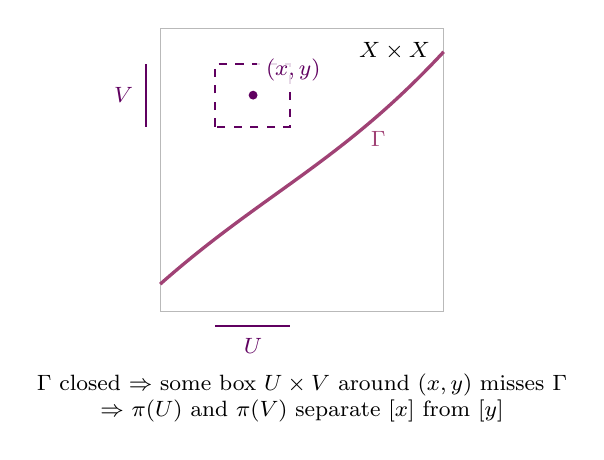
\begin{tikzpicture}[scale=1.0]
\draw[gray!55] (0,0) rectangle (3.6,3.6);
\node[font=\footnotesize,anchor=north east] at (3.55,3.55) {$X\times X$};
\draw[magenta!60!black,very thick] (0,0.35) .. controls (1.3,1.5) and (2.3,1.9) .. (3.6,3.3);
\node[magenta!60!black,font=\footnotesize,anchor=west] at (2.55,2.2) {$\Gamma$};
\draw[dashed,violet!75!black,thick] (0.7,2.35) rectangle (1.65,3.15);
\fill[violet!75!black] (1.18,2.75) circle (1.6pt);
\node[fill=white, fill opacity=0.85, text opacity=1, text=violet!75!black,font=\footnotesize,anchor=south west] at (1.22,2.8) {$(x,y)$};
\draw[violet!75!black,thick] (0.7,-0.18) -- (1.65,-0.18);
\node[violet!75!black,font=\footnotesize,below] at (1.18,-0.22) {$U$};
\draw[violet!75!black,thick] (-0.18,2.35) -- (-0.18,3.15);
\node[violet!75!black,font=\footnotesize,left] at (-0.22,2.75) {$V$};
\node[font=\footnotesize,align=center] at (1.8,-1.1) {$\Gamma$ closed $\Rightarrow$ some box $U\times V$ around $(x,y)$ misses $\Gamma$\\ $\Rightarrow$ $\pi(U)$ and $\pi(V)$ separate $[x]$ from $[y]$};
\end{tikzpicture}
\end{center}



\begin{rembox}[No Hausdorff Hypothesis on $X$]\label{rem:no-hausdorff-hypothesis-x}
Mid-statement, Uribe began to add the hypothesis ``assume $X$ is Hausdorff''---then stopped: ``actually, I don't need that.'' The final statement is correct as it stands: no separation assumption on $X$ is required, only openness of the relation. (Openness, moreover, is used only in the direction $\Leftarrow$; the direction $\Rightarrow$ holds for arbitrary equivalence relations, as the proof shows.)
\end{rembox}

\begin{corbox}[The Diagonal Criterion]\thmlabel{cor:diagonal-criterion}
A topological space $X$ is Hausdorff if and only if the diagonal $\Delta = \{(x,x) \mid x \in X\}$ is closed in $X \times X$.
\end{corbox}

\begin{proof}
Apply Theorem~\ref{thm:hausdorff-criterion} to the trivial relation, $x \sim y \iff x = y$. It is open, since every set is its own saturation. Its graph is $\Gamma = \Delta$. And $\pi : X \to X/{\sim}$ is a continuous open bijection, hence a homeomorphism, so $X/{\sim}$ is Hausdorff iff $X$ is. This classical characterization is the special case of the theorem with nothing identified; the theorem is its generalization to quotients.
\end{proof}
\begin{rembox}[This Is the Tool]\label{rem:this-tool}
Uribe (emphasized): ``this is going to be our tool for figuring out whether a quotient space is $T_2$.'' The workflow it suggests, and which the $\mathbb{CP}^n$ example below executes: (i) show the relation is open --- usually via the saturation slogan; (ii) show the graph is closed --- often by exhibiting $\Gamma$ as a preimage of a closed set, or as a compact set inside a Hausdorff space.
\end{rembox}

\begin{thmbox}[Second Countability of Open Quotients]\thmlabel{thm:2c-quotient}
If $\sim$ is an open equivalence relation and $X$ is second countable, then $X/{\sim}$ is second countable.
\leeref{no counterpart; a course result}
\end{thmbox}

\begin{proof}[Proof (one line in lecture --- ``project the countable basis'')]
$\pi : X \to X/{\sim}$ is a continuous surjection, and open because $\sim$ is; so Lemma~\ref{lem:open-surj-basis} applies and the image of a countable basis of $X$ is a countable basis of $X/{\sim}$.
\end{proof}

\textbf{Comparison with Lee.} Lee's Appendix~A has no counterpart to Theorems~\ref{thm:hausdorff-criterion} and~\ref{thm:2c-quotient}: in his book the Hausdorff property and second countability of $\mathbb{RP}^n$ and $\mathbb{CP}^n$ are checked example by example (Example~1.5, Problem~1-9). The course proves one criterion for all open quotients at once and then reuses it for orbit spaces (\ref{sec:actions}) and coset spaces (\ref{sec:homogeneous}) --- which is what makes the quotient thread a thread.

\begin{exbox}[The Line with Two Origins --- via the Criterion]\exlabel{ex:two-origins-criterion}
Let $X = (\mathbb{R} \times \{1\}) \cup (\mathbb{R} \times \{2\}) \subseteq \mathbb{R}^2$ with the subspace topology (two disjoint copies of $\mathbb{R}$), and $(x,1) \sim (x,2)$ for $x \neq 0$, as in Example~\ref{ex:two-origins-quotient}. The graph
\[
\Gamma = \{(a,b) \in X \times X \mid a = b\} \cup \{\, ((x,i),(x,j)) \mid x \neq 0,\ i \neq j \,\}
\]
is \emph{not} closed in $X \times X$: the points $\big((\tfrac1n, 1), (\tfrac1n, 2)\big)$ lie in $\Gamma$ for every $n$, and converge in $X \times X$ to $\big((0,1),(0,2)\big)$, which is not in $\Gamma$ (the two origins are distinct and are not identified, the identification being imposed only for $x \neq 0$). A closed set contains the limits of its convergent sequences, so $\Gamma$ is not closed.

The relation is open: the saturation of an open $U \subseteq X$ is $U \cup \sigma(U \setminus (\{0\} \times \{1,2\}))$, where $\sigma(x,i) = (x, 3-i)$ swaps the two copies---a homeomorphism of $X$---so the saturation is a union of two open sets. Theorem~\ref{thm:hausdorff-criterion} therefore applies and gives: $X/{\sim}$ is \emph{not} Hausdorff. This recovers Example~\ref{ex:two-origins} from the criterion rather than by separating the origins by hand.
\end{exbox}

PSet 1, Problem 2 asks for the non-closedness of $\Gamma$ directly. The sequence argument above needs no metrizability: in any topological space, if $z_n \to z$ with all $z_n$ in a closed set $C$, then $z \in C$ (otherwise the open set $X \setminus C$ would eventually contain the $z_n$).



The application of these criteria to complex projective space $\mathbb{CP}^n$ is collected in Section~\ref{sec:ex-cpn}.



% ============================================================================
% SECTION 4: THE REGULAR VALUE THEOREM
% ============================================================================
\section{The Regular Value Theorem}\label{sec:rvt}

\roadmark{Thread: equations}{Manifolds cut out as level sets. It sits in this chapter because the next one needs it: $\SL(n,\mathbb{R})$, $\Ogp(n)$ and $\Ugp(n)$ are level sets.}

\textit{Reference: Lee Appendix C (Inverse and Implicit Function Theorems); MATH 452. The theorem itself is PSet 1, Problem 6.}

\begin{rembox}[Why This Section]\label{rem:why-this-section-2}
\ref{sec:new-spaces}--\ref{sec:open-quotients} built manifolds out of manifolds. This section builds them out of \emph{equations}: given a smooth map $F$ on an open subset of $\mathbb{R}^{n+k}$, when is the solution set $\{F = c\}$ a topological manifold, and of what dimension? The answer --- whenever the $k$ equations are independent at every solution --- is the single most productive source of examples in the course. It produces the spheres, every classical matrix group (\ref{sec:topgroups}), and in its smooth form every example of Chapter~3. The machinery is multivariable calculus, and the one theorem taken on faith is the implicit function theorem.
\end{rembox}

\subsection{The Jacobian and the Rank Condition}\label{sub:jacobian}

\begin{defbox}[Jacobian and Rank]\deflabel{def:jacobian}
Let $F = (F_1, \ldots, F_m) : \mathbb{R}^N \to \mathbb{R}^m$ be $C^1$ and $p \in \mathbb{R}^N$. The \textbf{Jacobian matrix} of $F$ at $p$ is the $m \times N$ matrix of partial derivatives
\[
DF_p = \begin{pmatrix}
\dfrac{\partial F_1}{\partial x_1}(p) & \cdots & \dfrac{\partial F_1}{\partial x_N}(p) \\[2mm]
\vdots & & \vdots \\[1mm]
\dfrac{\partial F_m}{\partial x_1}(p) & \cdots & \dfrac{\partial F_m}{\partial x_N}(p)
\end{pmatrix},
\qquad \text{row } a = \nabla F_a(p),
\]
regarded as the linear map $DF_p : \mathbb{R}^N \to \mathbb{R}^m$, $v \mapsto DF_p\, v$. It is the derivative of $F$ at $p$: $F(p + v) = F(p) + DF_p\, v + o(|v|)$, and the chain rule for a curve reads $\frac{d}{dt} F(\gamma(t)) = DF_{\gamma(t)}\, \gamma'(t)$. For $m = 1$ the Jacobian is the single row $\nabla F(p)$, and $DF_p\, v = \nabla F(p) \cdot v$.

The \textbf{rank} of an $m \times N$ matrix is the dimension of its image in $\mathbb{R}^m$, equivalently the number of linearly independent rows (equivalently, columns). It is at most $\min(m, N)$. $DF_p$ has \textbf{rank $m$} (\textbf{full rank} when $N \ge m$) iff it is surjective onto $\mathbb{R}^m$, iff the $m$ gradients $\nabla F_1(p), \ldots, \nabla F_m(p)$ are linearly independent. For $m = 1$ this just says $\nabla F(p) \neq 0$; for $m = 2$ it says $\nabla F_1(p)$ and $\nabla F_2(p)$ are nonzero and not parallel.
\leeref{App.~C, \emph{Total and Partial Derivatives}}
\end{defbox}


\subsection{Regular Points and Regular Values}\label{sub:regular-values}

\begin{defbox}[Regular Point and Regular Value]\deflabel{def:regular-value}
Let $F : \mathbb{R}^N \to \mathbb{R}^m$ be $C^1$.
\begin{enumerate}
    \item A point $p \in \mathbb{R}^N$ is a \textbf{regular point} of $F$ if the Jacobian $DF_p : \mathbb{R}^N \to \mathbb{R}^m$ (Definition~\ref{def:jacobian}) is surjective, i.e.\ has rank $m$. Otherwise $p$ is a \textbf{critical point}.
    \item A value $c \in \mathbb{R}^m$ is a \textbf{regular value} of $F$ if every point of the level set $F^{-1}(c)$ is a regular point. Otherwise $c$ is a \textbf{critical value}. (If $F^{-1}(c) = \emptyset$, then $c$ is vacuously a regular value.)
\end{enumerate}
For scalar-valued $F$ ($m = 1$) the Jacobian is the row vector $\nabla F(p)$, and $p$ is a regular point iff $\nabla F(p) \neq 0$; so $c \in \mathbb{R}$ is a regular value iff $\nabla F$ vanishes nowhere on $F^{-1}(c)$.
\leeref{Ch.~5, p.~105, with the same convention that $c$ is regular when $F^{-1}(c) = \emptyset$}
\end{defbox}

\begin{rembox}[The Constraint $N \ge m$]\label{rem:constraint-n-m}
Regular points can exist only when $N \ge m$, and the case $N = m$ is special; both facts are made precise in Proposition~\ref{prop:regular-N-le-m}, once the regular value theorem is available. Geometrically, one cannot cut an $N$-dimensional space down by more than $N$ independent constraints and have anything left --- the dimension count $N - m$ would be negative. The boundary case $N = m$ belongs to the \emph{inverse} function theorem rather than the implicit one. The situation of interest below is $N = n^2$, $m = 1$.
\end{rembox}

\begin{exbox}[Regular and Critical Values of $x^2 + y^2$]\exlabel{ex:regular-critical-values-x2-y2}
Let $f(x,y) = x^2 + y^2$ on $\mathbb{R}^2$, so $\nabla f = (2x, 2y)$, which vanishes only at the origin. Then $c > 0$ is a regular value and $f^{-1}(c)$ is a circle, a $1$-manifold; $c = 0$ is a critical value and $f^{-1}(0) = \{(0,0)\}$ is a single point, not a $1$-manifold; $c < 0$ is vacuously regular. Note the logic: one critical point on the level set makes the value critical, while the value stays regular no matter how many critical points $f$ has \emph{off} that level set.
\end{exbox}

\begin{rembox}[Why the Notion Matters]\label{rem:why-notion-matters}
The definition is tailored to the Implicit Function Theorem: at a regular point of $F : \mathbb{R}^N \to \mathbb{R}^m$, the $m$ independent gradients $\nabla F_a(p)$ span an $m$-dimensional space of ``constraint directions,'' and one can solve the $m$ equations $F = c$ for $m$ of the coordinates as functions of the remaining $N - m$, so $F^{-1}(c)$ is locally a graph over the complementary $N - m$ directions. That is where the dimension $N - m$ comes from. For $\Ogp(n)$ the constraint is $gg^{\mathsf T} = I$, which is $m = \tfrac{n(n+1)}{2}$ scalar equations (the independent entries of a symmetric matrix), and the task is precisely to show these $m$ gradients are independent at every orthogonal $g$; this is done in Example~\ref{ex:On-smooth}. The general statement---\emph{if $c$ is a regular value of $F$, then $F^{-1}(c)$ is a topological (indeed smooth) manifold of dimension $N - m$}---is Theorem~\ref{thm:regular-value} (PSet 1, Problem 6); the $m = 1$ case is carried out for $\det$ in Proposition~\ref{prop:SL-loc-euc} below.
\end{rembox}


\begin{center}
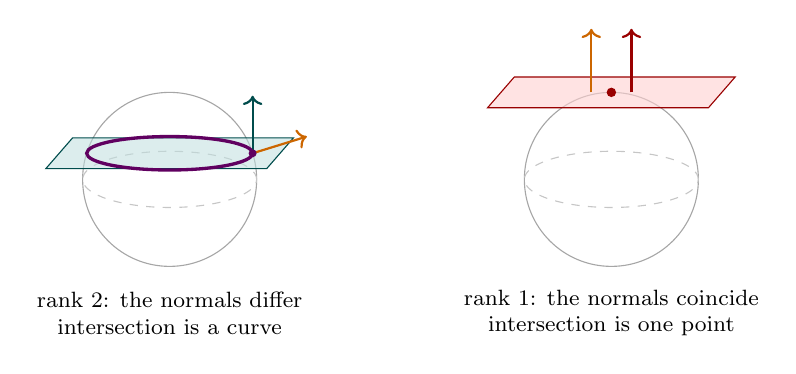
\begin{tikzpicture}[scale=0.85]
\draw[gray!70] (0,0) circle (1.3);
\draw[gray!45,dashed] (0,0) ellipse (1.3 and 0.42);
\fill[teal!25,opacity=0.55] (-1.85,0.16) -- (1.45,0.16) -- (1.85,0.62) -- (-1.45,0.62) -- cycle;
\draw[teal!60!black] (-1.85,0.16) -- (1.45,0.16) -- (1.85,0.62) -- (-1.45,0.62) -- cycle;
\draw[violet!75!black,very thick] (0,0.39) ellipse (1.24 and 0.25);
\draw[orange!80!black,->,thick] (1.24,0.39) -- (2.05,0.64);
\draw[teal!60!black,->,thick] (1.24,0.39) -- (1.24,1.25);
\fill[violet!75!black] (1.24,0.39) circle (1.7pt);
\node[font=\footnotesize,align=center] at (0,-2.0) {rank $2$: the normals differ\\ intersection is a curve};
\begin{scope}[xshift=6.6cm]
\draw[gray!70] (0,0) circle (1.3);
\draw[gray!45,dashed] (0,0) ellipse (1.3 and 0.42);
\fill[red!18,opacity=0.6] (-1.85,1.07) -- (1.45,1.07) -- (1.85,1.53) -- (-1.45,1.53) -- cycle;
\draw[red!60!black] (-1.85,1.07) -- (1.45,1.07) -- (1.85,1.53) -- (-1.45,1.53) -- cycle;
\draw[orange!80!black,->,thick] (-0.3,1.3) -- (-0.3,2.25);
\draw[red!60!black,->,thick] (0.3,1.3) -- (0.3,2.25);
\fill[red!60!black] (0,1.3) circle (2pt);
\node[font=\footnotesize,align=center] at (0,-2.0) {rank $1$: the normals coincide\\ intersection is one point};
\end{scope}
\end{tikzpicture}
\end{center}

The figure is the case $N = 3$, $m = 2$: two equations in $\mathbb{R}^3$, each level set a surface, the common level set their intersection. On the left the sphere $x^2+y^2+z^2 = 1$ meets the plane $z = c$ with $|c| < 1$ transversally, the two gradients at a point of intersection are independent, the Jacobian has rank $2$, and the intersection is a curve of dimension $3 - 2 = 1$. On the right, $F = (x^2+y^2+z^2-1,\, z-1)$: both components have nonvanishing gradient, but at the tangency $(0,0,1)$ they are parallel, so
\[
DF_{(0,0,1)} = \begin{pmatrix} 0 & 0 & 2 \\ 0 & 0 & 1 \end{pmatrix}
\]
has rank $1$, and $F^{-1}(\vec 0)$ is the single point $(0,0,1)$ rather than the predicted curve. This is what the scalar case $m = 1$ cannot show: there the hypothesis reads ``$\nabla F \neq 0$'' and looks like a condition on one function, whereas it is really a condition on the gradients \emph{jointly}.


\subsection{The Implicit Function Theorem}\label{sub:ift}

\begin{thmbox}[Implicit Function Theorem --- Lee Theorem C.40]\thmlabel{thm:ift-general}
Let $U \subseteq \mathbb{R}^n \times \mathbb{R}^k$ be an open subset, with standard coordinates written $(x, y) = (x^1, \ldots, x^n, y^1, \ldots, y^k)$. Suppose $\Phi : U \to \mathbb{R}^k$ is smooth, $(a, b) \in U$, and $c = \Phi(a,b)$. If the $k \times k$ matrix
\[
\left( \frac{\partial \Phi^i}{\partial y^j}(a, b) \right)_{1 \le i, j \le k}
\]
is nonsingular, then there exist neighborhoods $V_0 \subseteq \mathbb{R}^n$ of $a$ and $W_0 \subseteq \mathbb{R}^k$ of $b$ and a smooth function $F : V_0 \to W_0$ such that $\Phi^{-1}(c) \cap (V_0 \times W_0)$ is the graph of $F$; that is, for $(x,y) \in V_0 \times W_0$,
\[
\Phi(x, y) = c \iff y = F(x).
\]
\leeref{Theorem C.40}
\end{thmbox}

\begin{proof}[Proof (sketch)]
Lee deduces this from the Inverse Function Theorem (Theorem~\ref{thm:inverse-function}; Lee, Theorem C.34), applied to the auxiliary map $(x,y) \mapsto (x, \Phi(x,y))$, whose total derivative is block lower triangular with nonsingular diagonal blocks $I_n$ and $(\partial\Phi^i/\partial y^j)$. Both theorems are proved in MATH 452; Lee's proofs are in Appendix C.
\end{proof}

\begin{rembox}[Which Variables Are Solved For]\label{rem:which-variables-solved}
The theorem does not say the level set is a graph over some canonical set of coordinates: it says that \emph{if} the $k$ coordinates $y$ are ones for which the square block $(\partial\Phi^i/\partial y^j)$ is invertible, \emph{then} those $y$ can be solved for in terms of the remaining $n$. Since $D\Phi_{(a,b)}$ has rank $k$ exactly when \emph{some} $k$ of its $n + k$ columns are independent, a regular point always admits such a splitting---after permuting coordinates. That permutation is the ``WLOG'' step in the proof of Proposition~\ref{prop:SL-loc-euc} below.
\end{rembox}

We need only the scalar case $k = 1$. Write $N = n^2$ and points of $\mathbb{R}^N$ as $x = (x', x_N)$ with $x' \in \mathbb{R}^{N-1}$.

\begin{corbox}[Implicit Function Theorem --- Scalar Case]\thmlabel{thm:ift}
Let $F : \mathbb{R}^N \to \mathbb{R}$ be smooth, let $a = (a', a_N)$ with $F(a) = c$, and suppose $\dfrac{\partial F}{\partial x_N}(a) \neq 0$. Then there exist an open set $W' \subseteq \mathbb{R}^{N-1}$ containing $a'$, an open interval $J \subseteq \mathbb{R}$ containing $a_N$, and a smooth function $h : W' \to J$ with $h(a') = a_N$ such that for all $(x', x_N) \in W' \times J$,
\[
F(x', x_N) = c \iff x_N = h(x').
\]
\leeref{Theorem C.40 with $k = 1$}
\end{corbox}

\begin{proof}
Theorem~\ref{thm:ift-general} with $n = N - 1$, $k = 1$, $\Phi = F$: the $1 \times 1$ matrix $(\partial F/\partial x_N(a))$ is nonsingular precisely when $\partial F/\partial x_N(a) \neq 0$. Set $h = F$ in Lee's notation, and note $h(a') = a_N$ because $(a', a_N)$ lies in the level set and in $V_0 \times W_0$.
\end{proof}


\subsection{The Regular Value Theorem}\label{sub:rvt-proper}

\begin{thmbox}[Regular Value Theorem]\thmlabel{thm:regular-value}
Let $F : \mathbb{R}^{n+k} \to \mathbb{R}^k$ be smooth and suppose $\vec 0 \in \mathbb{R}^k$ is a regular value of $F$, i.e.\ the Jacobian $F'(p)$ has rank $k$ at every $p \in X := F^{-1}(\vec 0)$. Then $X$, with the subspace topology, is a topological manifold of dimension $n$.
\leeref{Example 1.32 and Corollary 5.14}
\end{thmbox}

\begin{proof}[Proof (PSet 1, Problem 6)]
\emph{Hausdorff and second countable.} $X$ is a subspace of $\mathbb{R}^{n+k}$, so both properties are inherited (Theorem~\ref{thm:subspace-inherit}).

\emph{Locally Euclidean.} Fix $p \in X$.

\emph{Step 1 (relabelling the coordinates).} $F'(p)$ is a $k \times (n+k)$ matrix of rank $k$, so $k$ of its $n+k$ columns are linearly independent. Let $\rho : \mathbb{R}^{n+k} \to \mathbb{R}^{n+k}$ be the coordinate permutation carrying those $k$ positions to the last $k$, and put $\widetilde F = F \circ \rho^{-1}$. Then $\widetilde F$ is smooth, $\widetilde F^{-1}(\vec 0) = \rho(X)$, and $\widetilde F'(\rho(p)) = F'(p)\,\rho^{-1}$ is $F'(p)$ with its columns permuted, so its last $k$ columns are independent. As $\rho$ restricts to a homeomorphism $X \to \rho(X)$, and local Euclideanness is a topological property, we may replace $(X, F, p)$ by $(\rho(X), \widetilde F, \rho(p))$: WLOG, writing the coordinates as $(x,y) \in \mathbb{R}^n \times \mathbb{R}^k$, the $k \times k$ matrix $\big(\partial F^i/\partial y^j (p)\big)$ --- the last $k$ columns of $F'(p)$ --- is nonsingular.

\emph{Step 2 (the implicit function theorem).} Write $p = (a,b)$. By Theorem~\ref{thm:ift-general} applied to $\Phi = F$ on $U = \mathbb{R}^{n+k}$ with $c = \vec 0$, there are neighborhoods $V_0 \subseteq \mathbb{R}^n$ of $a$ and $W_0 \subseteq \mathbb{R}^k$ of $b$ and a smooth $G : V_0 \to W_0$ with
\[
F(x,y) = \vec 0 \iff y = G(x) \qquad \text{for } (x,y) \in V_0 \times W_0. \tag{$\ast$}
\]

\emph{Step 3 (the level set is locally a graph).} Put $U_p = X \cap (V_0 \times W_0)$, an open neighborhood of $p$ in $X$. By $(\ast)$,
\[
U_p = \{\, (x, G(x)) \mid x \in V_0 \,\} :
\]
``$\supseteq$'' because $(x,G(x)) \in V_0 \times W_0$ satisfies $F = \vec 0$, ``$\subseteq$'' because a point of $U_p$ over $x$ has second coordinate $G(x)$. The maps
\[
\varphi : U_p \to V_0,\ \varphi(x,y) = x, \qquad \psi : V_0 \to U_p,\ \psi(x) = (x, G(x))
\]
are mutually inverse; $\varphi$ is continuous as a restriction of the projection, and $\psi$ is continuous because its two components $\mathrm{id}$ and $G$ are (Theorem~\ref{thm:univ-product} and Proposition~\ref{prop:univ-subspace}). So $\varphi$ is a homeomorphism onto the open set $V_0 \subseteq \mathbb{R}^n$, and Proposition~\ref{prop:open-charts} gives local Euclideanness of dimension $n$ at $p$.
\end{proof}

\begin{corbox}[Open Domains and Arbitrary Values]\thmlabel{cor:rvt-open}
Let $W \subseteq \mathbb{R}^{n+k}$ be open, $F : W \to \mathbb{R}^k$ smooth, and $c \in \mathbb{R}^k$ a regular value of $F$ --- Definition~\ref{def:regular-value}, applied to $F$ on $W$: the Jacobian $F'(p)$ has rank $k$ at every $p \in F^{-1}(c)$. Then $F^{-1}(c)$, with the subspace topology, is a topological manifold of dimension $n$.
\end{corbox}

\begin{proof}
The proof of Theorem~\ref{thm:regular-value} is local, and uses the domain and the value only through the implicit function theorem, which is stated for an arbitrary open set and value (Theorem~\ref{thm:ift-general}). Repeat it with $W$ in place of $\mathbb{R}^{n+k}$ and $c$ in place of $\vec 0$: the permutation $\rho$ of Step~1 carries $W$ to the open set $\rho(W)$; Step~2 applies Theorem~\ref{thm:ift-general} on $U = \rho(W)$ at the value $c$; Step~3 is unchanged. Hausdorffness and second countability are inherited from $\mathbb{R}^{n+k}$ as before.
\end{proof}

This is the form needed on manifolds, where a chart has an open subset of Euclidean space as its image, not the whole space. The general version, for maps between manifolds and with the smooth structure and the tangent space included, is Theorem~\ref{thm:rvt-manifolds} (Lecture~12).

\textbf{Comparison with Lee.} Lee meets level sets twice. Example~1.32 builds graph charts for the level set of a single function with nonvanishing gradient, and Corollary~5.14 proves, via the constant-rank theorem, that every regular level set is a properly embedded submanifold. The course takes the direct route of Example~1.32 in every codimension, using the implicit function theorem, and obtains the smooth structure separately (Proposition~\ref{prop:level-set-smooth}).


\begin{center}
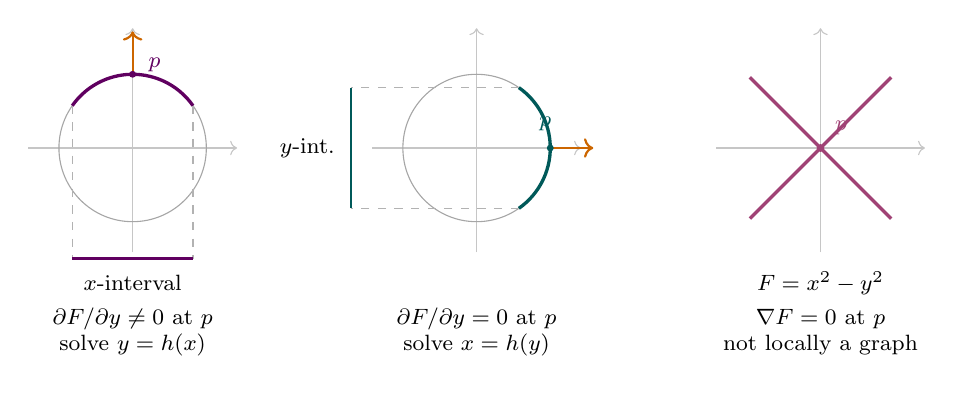
\begin{tikzpicture}[scale=0.78]
\foreach \dx in {0, 5.6, 11.2} {
  \draw[gray!45,->] (\dx-1.7,0) -- (\dx+1.7,0);
  \draw[gray!45,->] (\dx,-1.7) -- (\dx,1.95);
}
\draw[gray!70] (0,0) circle (1.2);
\draw[violet!75!black,very thick] (35:1.2) arc (35:145:1.2);
\draw[dashed,gray!60] (145:1.2) -- ({1.2*cos(145)},-1.8);
\draw[dashed,gray!60] (35:1.2) -- ({1.2*cos(35)},-1.8);
\draw[violet!75!black,thick] ({1.2*cos(145)},-1.8) -- ({1.2*cos(35)},-1.8);
\draw[orange!80!black,->,thick] (0,1.2) -- (0,1.9);
\fill[violet!75!black] (0,1.2) circle (1.6pt);
\node[violet!75!black,font=\footnotesize,anchor=west] at (0.1,1.36) {$p$};
\node[font=\footnotesize] at (0,-2.2) {$x$-interval};
\node[font=\footnotesize,align=center] at (0,-3.0) {$\partial F/\partial y\neq0$ at $p$\\ solve $y=h(x)$};
\draw[gray!70] (5.6,0) circle (1.2);
\draw[teal!70!black,very thick] ([shift={(5.6,0)}]-55:1.2) arc (-55:55:1.2);
\draw[dashed,gray!60] ([shift={(5.6,0)}]55:1.2) -- (3.55,{1.2*sin(55)});
\draw[dashed,gray!60] ([shift={(5.6,0)}]-55:1.2) -- (3.55,{-1.2*sin(55)});
\draw[teal!70!black,thick] (3.55,{-1.2*sin(55)}) -- (3.55,{1.2*sin(55)});
\draw[orange!80!black,->,thick] (6.8,0) -- (7.5,0);
\fill[teal!70!black] (6.8,0) circle (1.6pt);
\node[teal!70!black,font=\footnotesize,anchor=south] at (6.72,0.12) {$p$};
\node[font=\footnotesize,anchor=east] at (3.45,0) {$y$-int.};
\node[font=\footnotesize,align=center] at (5.6,-3.0) {$\partial F/\partial y=0$ at $p$\\ solve $x=h(y)$};
\draw[magenta!60!black,very thick] (10.05,-1.15) -- (12.35,1.15);
\draw[magenta!60!black,very thick] (10.05,1.15) -- (12.35,-1.15);
\fill[magenta!60!black] (11.2,0) circle (1.8pt);
\node[magenta!60!black,font=\footnotesize,anchor=south west] at (11.28,0.06) {$p$};
\node[font=\footnotesize] at (11.2,-2.2) {$F=x^2-y^2$};
\node[font=\footnotesize,align=center] at (11.2,-3.0) {$\nabla F=0$ at $p$\\ not locally a graph};
\end{tikzpicture}
\end{center}

The scalar case $N = 2$, $m = 1$, where every step of the proof is visible at once. \emph{Left:} $F = x^2+y^2-1$; at a point off the horizontal axis $\partial F/\partial y \neq 0$, so the implicit function theorem solves $y = h(x) = \sqrt{1-x^2}$ and the thick arc is the graph over the $x$-interval beneath it --- the chart is ``project to $x$,'' which is exactly $\varphi_2$ of Example~\ref{ex:circle-four}. \emph{Middle:} at $(1,0)$ that partial vanishes and the curve is vertical, so no interval of $x$ works; but $\partial F/\partial x \neq 0$, so one solves $x = h(y)$ and projects to $y$ instead. That switch is the permutation-of-coordinates step in the proof, and the picture shows it is not a technicality: which coordinate can be solved for changes from point to point. \emph{Right:} at a critical point the conclusion fails --- near the origin $\{x^2 = y^2\}$ is two crossing lines, a graph over neither axis.

\begin{rembox}[Reading the Dimension]\label{rem:reading-dimension}
The level set of $k$ independent equations in $\mathbb{R}^{n+k}$ has dimension $(n+k) - k = n$: each independent constraint costs one dimension. The independence is exactly the rank condition, and it is needed at every point of the level set, not just at one --- that is what ``regular \emph{value}'' means (Definition~\ref{def:regular-value}). The theorem is the general form of the computation carried out for $\SL(n,\mathbb{R})$ in \S\ref{sub:classical-manifolds}, the case $k = 1$, $n + k = n^2$; the smooth version, giving $X$ a smooth structure rather than just a topology, comes in Chapter 3.
\end{rembox}


\begin{propbox}[Regular Points When $N \le m$]\thmlabel{prop:regular-N-le-m}
Let $W \subseteq \mathbb{R}^N$ be open and $F : W \to \mathbb{R}^m$ smooth.
\begin{enumerate}
    \item $\operatorname{rank} DF_p \le \min(m, N)$ at every $p$. So if $N < m$, every point of $W$ is critical, and $c$ is a regular value if and only if $F^{-1}(c) = \emptyset$.
    \item If $N = m$, then $p$ is a regular point if and only if $\det DF_p \ne 0$, and every regular level set $F^{-1}(c)$ is discrete: each of its points is isolated.
\end{enumerate}
\end{propbox}

\begin{proof}
(1) An $m \times N$ matrix has at most $\min(m,N)$ independent rows. If $N < m$, the rank is at most $N < m$, so $DF_p$ is never surjective and no point is regular; the condition defining a regular value then holds exactly when there is nothing to check. (2) A square matrix has maximal rank iff it is invertible. If $c$ is a regular value, Theorem~\ref{thm:regular-value} applies with $n = 0$ and $k = m$, so $F^{-1}(c)$ is a manifold of dimension $0$, hence discrete by Proposition~\ref{prop:zero-manifolds}.
\end{proof}

\begin{exbox}[A Level Set in $\mathbb{R}^4$]\exlabel{ex:qr-level-set}
\textit{(Qualifying Review, August 2013; Assignment 2, Problem 3.)} Define
\[
F : \mathbb{R}^4 \to \mathbb{R}^2, \qquad F(x,y,u,v) = \big(x^2 - y^2 - u^2 + v^2 + 2u,\ \ 2xy - 2uv + 2v\big),
\]
and $M = F^{-1}(-1,0)$. Then $(-1,0)$ is a regular value of $F$, so $M$ is a manifold of dimension $2$; and at $x_0 = (0,1,0,0) \in M$,
\[
\ker F'(x_0) = \operatorname{span}\{(1,0,0,-1),\ (0,1,1,0)\}.
\]
\end{exbox}

\begin{proof}[Working out the example]
\emph{Step 1: the Jacobian.} Writing $a = 2x$, $b = 2y$, $c = 2 - 2u$, $d = 2v$,
\[
F'(p) = \begin{pmatrix} 2x & -2y & 2 - 2u & 2v \\ 2y & 2x & -2v & 2 - 2u \end{pmatrix}
= \begin{pmatrix} a & -b & c & d \\ b & a & -d & c \end{pmatrix}.
\]

\emph{Step 2: where the rank drops.} A $2 \times 4$ matrix has rank $< 2$ iff its rows are linearly dependent. If the second row is $0$ then $a = b = c = d = 0$. Otherwise the first is $\gamma$ times the second for some real $\gamma$; comparing entries, $a = \gamma b$ and $-b = \gamma a = \gamma^2 b$, so $b(1+\gamma^2) = 0$, whence $b = 0 = a$; likewise $c = -\gamma d$ and $d = \gamma c = -\gamma^2 d$ force $d = 0 = c$ --- so this case is vacuous. Either way $a = b = c = d = 0$, i.e.\ $p = p_0 := (0,0,1,0)$: the rank is $2$ everywhere except at the single point $p_0$.

\emph{Step 3: the bad point misses the level set.} $F(p_0) = (0 - 0 - 1 + 0 + 2,\ 0) = (1,0) \neq (-1,0)$, so $p_0 \notin M$ and $F'(p)$ has rank $2$ at every $p \in M$: $(-1,0)$ is a regular value.

\emph{Step 4: the manifold.} By Theorem~\ref{thm:regular-value}, $M$ is a topological manifold of dimension $4 - 2 = 2$, smooth by Proposition~\ref{prop:level-set-smooth}.

\emph{Step 5: the kernel at $x_0$.} First $F(0,1,0,0) = (-1,0)$, so $x_0 \in M$. At $x_0$,
\[
F'(x_0) = \begin{pmatrix} 0 & -2 & 2 & 0 \\ 2 & 0 & 0 & 2 \end{pmatrix},
\qquad
F'(x_0)\begin{pmatrix} x \\ y \\ u \\ v \end{pmatrix} = \begin{pmatrix} -2y + 2u \\ 2x + 2v \end{pmatrix},
\]
which vanishes iff $u = y$ and $v = -x$. So $\ker F'(x_0) = \{(x, y, y, -x)\}$, spanned by the two displayed vectors, of dimension $2 = \dim M$ as it must be. By Theorem~\ref{thm:tangent-kernel} this kernel is the geometric tangent space $T^{\geo}_{x_0}M$.
\end{proof}

\begin{rembox}\label{rem:rvt}
\textbf{The workflow.} Every problem of this type runs the same five steps: (i) compute the Jacobian; (ii) find the locus where its rank drops; (iii) check that this locus \emph{misses the level set}; (iv) read off the dimension; (v) compute the kernel. Step (iii) is the one most often skipped, and it is the point of the definition: the rank may drop anywhere at all, so long as it does not drop \emph{on} $F^{-1}(c)$. Here it drops at exactly one point of $\mathbb{R}^4$, which happens to lie on a different level set.
\end{rembox}

\textbf{On the word ``submanifold.''} The problem asks to show $M$ is a \emph{submanifold} of $\mathbb{R}^4$, a notion not yet defined in the course; Assignment~2's own background defers it (``after the theory of submanifolds is developed''). What has been proved is that $M$ is a smooth manifold, and that its topology is the subspace topology from $\mathbb{R}^4$.

\subsection{Holomorphic Level Sets}\label{sub:holomorphic-level-sets}

Step~2 of Example~\ref{ex:qr-level-set} found something it did not look for: the rank of $F'(p)$ is either $2$ or $0$, and never $1$. That is not a coincidence of this particular $F$. With $z = x + iy$ and $w = u + iv$,
\[
F = (\operatorname{Re} f,\ \operatorname{Im} f), \qquad f(z,w) = z^2 - w^2 + 2w,
\]
as expanding $f$ shows; so $F$ is a complex polynomial in disguise, and its rank behaviour is forced by the complex structure. This subsection makes that precise. Throughout, $\mathbb{C}^m \cong \mathbb{R}^{2m}$ as in Definition~\ref{def:complex-groups}.

\begin{center}
\begin{tikzcd}[row sep=2.6em, column sep=3em]
\mathbb{C}^2 \arrow[r, "f"] \arrow[d, "\cong"'] & \mathbb{C} \arrow[d, "\cong"] \\
\mathbb{R}^4 \arrow[r, "F"'] & \mathbb{R}^2
\end{tikzcd}
\qquad\qquad
\begin{tikzcd}[row sep=2.6em, column sep=3em]
\mathbb{C}^2 \arrow[r, "f'(p)"] \arrow[d, "\cong"'] & \mathbb{C} \arrow[d, "\cong"] \\
\mathbb{R}^4 \arrow[r, "F'(p)"'] & \mathbb{R}^2
\end{tikzcd}
\end{center}

Left, the map; right, its derivative at a point. The vertical arrows are the identifications of Definition~\ref{def:complex-groups}. On the right, the top arrow is the complex gradient $(2z,\ 2-2w)$, a $1 \times 2$ complex matrix, and the bottom arrow is the real $2 \times 4$ Jacobian of Example~\ref{ex:qr-level-set}. Everything that follows is about what the top row forces on the bottom one.

\begin{defbox}[Holomorphic Map]\deflabel{def:holomorphic}
Let $W \subseteq \mathbb{C}^N$ be open. A map $F : W \to \mathbb{C}^m$ is \textbf{holomorphic} if it is $C^1$ as a map between open subsets of $\mathbb{R}^{2N}$ and $\mathbb{R}^{2m}$ and its real derivative $DF_p : \mathbb{C}^N \to \mathbb{C}^m$ is $\mathbb{C}$-linear at every $p \in W$. The $\mathbb{C}$-linear map $DF_p$ is then written $F'(p)$, the \textbf{complex Jacobian}, an $m \times N$ complex matrix of partial derivatives $\partial F_a / \partial z_b$.
\end{defbox}

\begin{rembox}\label{rem:rvt-2}
$\mathbb{C}$-linearity of $DF_p$ is the Cauchy--Riemann condition. For $N = m = 1$: multiplication by $\alpha = a + ib$ sends $h = h_1 + i h_2$ to $(a h_1 - b h_2) + i(b h_1 + a h_2)$, so as a real $2 \times 2$ matrix
\[
h \mapsto \alpha h \quad\text{is}\quad \begin{pmatrix} a & -b \\ b & a \end{pmatrix}.
\]
A real $2 \times 2$ matrix is of this form iff it commutes with multiplication by $i$. Polynomials in $z_1, \ldots, z_N$ (with no $\bar z_j$) are holomorphic, by the product and chain rules; maps involving complex conjugation generally are not.
\end{rembox}

\begin{lembox}[Real Rank of a Complex-Linear Map]\thmlabel{lem:real-rank-complex}
Let $A : \mathbb{C}^N \to \mathbb{C}^m$ be $\mathbb{C}$-linear of complex rank $r$. Regarded as an $\mathbb{R}$-linear map $\mathbb{R}^{2N} \to \mathbb{R}^{2m}$, it has real rank $2r$. In particular the real rank of a $\mathbb{C}$-linear map is always even.
\end{lembox}

\begin{proof}
The image of $A$ is a complex subspace $V$ of complex dimension $r$; it suffices to show $\dim_{\mathbb{R}} V = 2r$. Let $v_1, \ldots, v_r$ be a complex basis of $V$. Then $v_1, iv_1, \ldots, v_r, iv_r$ span $V$ over $\mathbb{R}$, since $\sum_j c_j v_j = \sum_j \big(\operatorname{Re} c_j\, v_j + \operatorname{Im} c_j\,(i v_j)\big)$; and they are $\mathbb{R}$-independent, since $\sum_j (a_j v_j + b_j\, i v_j) = 0$ with $a_j, b_j$ real says $\sum_j (a_j + i b_j) v_j = 0$, forcing every $a_j + i b_j = 0$. So they form a real basis of $2r$ vectors.
\end{proof}

\begin{corbox}[Holomorphic Regular Value Theorem]\thmlabel{cor:holomorphic-rvt}
Let $W \subseteq \mathbb{C}^{n+k}$ be open, $F : W \to \mathbb{C}^k$ holomorphic, and $c \in \mathbb{C}^k$ such that the complex Jacobian $F'(p)$ has complex rank $k$ at every $p \in F^{-1}(c)$. Then $F^{-1}(c)$ is a manifold of \emph{real} dimension $2n$, smooth by Proposition~\ref{prop:level-set-smooth}. Moreover, for any holomorphic $F$ the real rank of $DF_p$ is even at every point; for $k = 1$ it is $0$ or $2$. And for $p \in F^{-1}(c)$ the kernel of $F'(p)$ is a complex subspace of $\mathbb{C}^{n+k}$; by Theorem~\ref{thm:tangent-kernel} it is the geometric tangent space $T^{\geo}_p F^{-1}(c)$.
\leeref{no counterpart; from Assignment 2}
\end{corbox}

\begin{proof}
By Lemma~\ref{lem:real-rank-complex}, complex rank $k$ means real rank $2k$, which is the maximal rank for a real map $\mathbb{R}^{2n+2k} \to \mathbb{R}^{2k}$. So $c$ is a regular value of $F$ regarded as a real map, and Theorem~\ref{thm:regular-value} gives a manifold of dimension $(2n+2k) - 2k = 2n$. Evenness of the rank is the lemma again. The kernel of a $\mathbb{C}$-linear map is closed under multiplication by $i$, hence a complex subspace.
\end{proof}

\begin{rembox}[The Example Re-read]\label{rem:example-re-read}
For $f(z,w) = z^2 - w^2 + 2w$ the complex Jacobian is the row $(2z,\ 2 - 2w)$. In the notation of Example~\ref{ex:qr-level-set}, $2z = a + ib$ and $2 - 2w = c - id$, and the $\mathbb{C}$-linear functional $(h, k) \mapsto (a+ib)h + (c-id)k$ has real and imaginary parts
\[
\operatorname{Re}:\ (a,\ -b,\ c,\ d), \qquad \operatorname{Im}:\ (b,\ a,\ -d,\ c)
\]
--- exactly the two rows computed in Step~1. So the case analysis of Step~2 was Lemma~\ref{lem:real-rank-complex} in disguise: the real rank is $2$ precisely when the complex gradient $(2z, 2-2w)$ is nonzero, i.e.\ away from $(z,w) = (0,1)$, and $0$ there, never $1$.

The kernel is complex too. At $x_0$, i.e.\ $(z,w) = (i, 0)$, the complex gradient is $(2i, 2)$, and its kernel is the complex line $\{2i\,h + 2k = 0\} = \{k = -i h\}$. Writing $h = h_1 + i h_2$ and $k = k_1 + i k_2$, the condition $k = -ih = h_2 - i h_1$ reads $k_1 = h_2$, $k_2 = -h_1$ --- which is $\{(x,y,y,-x)\}$ from Step~5. As Corollary~\ref{cor:holomorphic-rvt} predicts, it is a complex subspace.
\end{rembox}

\begin{rembox}[The Contrast with the Unitary Group]\label{rem:contrast-unitary-group}
The map $F(g) = gg^*$ presenting $\Ugp(n)$ (Assignment~2, Problem~4) involves $\bar g$ and is \emph{not} holomorphic: its derivative $h \mapsto hg^* + gh^*$ satisfies $DF_g(ih) = i\,hg^* - i\,gh^*$, which is not $i\,DF_g(h)$ in general. So Corollary~\ref{cor:holomorphic-rvt} is unavailable, and one is forced to regard $\Mat(n,\mathbb{C})$ and the Hermitian matrices as \emph{real} vector spaces --- which is exactly why that problem insists on it. The outcome shows the difference: $\dim \Ugp(n) = n^2$ is odd for odd $n$ (for instance $\Ugp(1) = S^1$ has dimension $1$), which no holomorphic regular level set can be.
\end{rembox}

\begin{exbox}[The Level Set Is a Cylinder]\exlabel{ex:qr-cylinder}
The regular value theorem says that $M$ of Example~\ref{ex:qr-level-set} is a $2$-manifold, but not which one. In fact $M$ is homeomorphic to $\mathbb{C}^\times$, hence to the cylinder $S^1 \times \mathbb{R}$.
\end{exbox}

\begin{proof}
In complex coordinates, completing the square,
\[
M = \{z^2 - (w-1)^2 = -2\} = \{(z - w + 1)(z + w - 1) = -2\}.
\]
The maps
\[
M \to \mathbb{C}^\times,\ \ (z,w) \mapsto s = z - w + 1, \qquad\qquad
\mathbb{C}^\times \to M,\ \ s \mapsto \Big(\tfrac12\big(s - \tfrac{2}{s}\big),\ 1 - \tfrac12\big(s + \tfrac{2}{s}\big)\Big),
\]
are continuous (indeed holomorphic) and mutually inverse, because the second factor $z + w - 1 = -2/s$ is determined by the first. So $M \cong \mathbb{C}^\times$. And $\mathbb{C}^\times \cong S^1 \times \mathbb{R}$ via $s \mapsto \big(s/|s|,\ \log|s|\big)$. The base point $x_0 = (0,1,0,0)$, i.e.\ $(z,w) = (i,0)$, corresponds to $s = 1+i$.
\end{proof}

\begin{center}
\begin{tikzcd}[column sep=6.5em]
M \arrow[r, shift left=0.8ex, "{(z,w) \,\mapsto\, z-w+1}"] & \mathbb{C}^\times \arrow[l, shift left=0.8ex, "{s \,\mapsto\, (z(s),\, w(s))}"] \arrow[r, "\cong"] & S^1 \times \mathbb{R}
\end{tikzcd}
\end{center}

$M$ upstairs in $\mathbb{C}^2$, the parameter $s$ downstairs in $\mathbb{C}^\times$, and polar coordinates $s \mapsto (s/|s|, \log|s|)$ to the cylinder. The two arrows on the left are mutually inverse, so $s$ is a single chart covering all of $M$ --- something the regular value theorem, whose charts are local graphs, never promises.


% ============================================================================
% SECTION: EXAMPLE: SPHERES
% ============================================================================

\section{Spheres}\label{sec:ex-spheres}

\roadmark{Thread: examples}{The sphere, the first manifold of the course, in one place: $S^2$ by hemisphere charts, every $S^n$ by the same argument, and two overlapping charts whose transition map is already smooth.}

The sphere through the course: a topological manifold with hemisphere charts in Section~\ref{sec:ex-spheres}; the homogeneous space $\SO(3)/\SO(2)$ in Example~\ref{ex:s2-homogeneous}; the Riemann sphere $\mathbb{CP}^1$ in Proposition~\ref{prop:cp1-sphere}; its geometric tangent spaces in Example~\ref{ex:tangent-sphere} and its transverse intersection with a plane in Example~\ref{ex:sphere-plane-transverse}; the double cover $S^n \to \mathbb{RP}^n$ and the Hopf fibration $S^{2n+1} \to \mathbb{CP}^n$ in Section~\ref{sec:ex-hopf}; and $S^3 = \mathrm{SU}(2)$ in Proposition~\ref{prop:s3-su2}.

\begin{exbox}[$S^2$ is a Topological $2$-Manifold]\exlabel{ex:s2-manifold}
Let $S^2 = \{x \in \mathbb{R}^3 \mid |x| = 1\}$ with the subspace topology.
\begin{itemize}
    \item \textit{$T_2$ and second countable:} $S^2$ is a metric space (restriction of the Euclidean metric), hence $T_2$; and a subspace of a second countable space is second countable (intersect a countable basis of $\mathbb{R}^3$ with $S^2$).
    \item \textit{Locally Euclidean:} let $p = (p_1, p_2, p_3) \in S^2$. Since $|p| = 1$, some coordinate of $p$ is nonzero. Upon relabeling coordinates (and possibly replacing $z$ by $-z$), we may assume \textbf{WLOG that the $z$-coordinate of $p$ is positive}. Let
    \[
    U = \{(x, y, z) \in S^2 \mid z > 0\} \quad \text{(the open northern hemisphere)},
    \]
    \[
    \varphi : U \to \mathbb{R}^2, \qquad (x, y, z) \mapsto (x, y).
    \]
    $U$ is open in $S^2$ (preimage of $(0, \infty)$ under the continuous coordinate function $z$), and $p \in U$.

    \textbf{Claim:} $\varphi$ is a homeomorphism of $U$ onto the open unit disk $D = \{(x, y) \mid x^2 + y^2 < 1\} \subseteq \mathbb{R}^2$.
\end{itemize}
\leeref{Example 1.4}
\end{exbox}

\begin{proof}[Proof of Claim (not given in lecture)]
\emph{Image:} for $(x, y, z) \in U$, $x^2 + y^2 = 1 - z^2 < 1$ since $0 < z \le 1$, so $\varphi(U) \subseteq D$. Conversely, for $(x, y) \in D$, the point $(x, y, \sqrt{1 - x^2 - y^2})$ lies in $U$ and maps to $(x, y)$; so $\varphi(U) = D$.

\emph{Injective:} if $(x, y, z), (x, y, z') \in U$, then $z = \sqrt{1 - x^2 - y^2} = z'$, using $z, z' > 0$.

\emph{Continuous with continuous inverse:} $\varphi$ is the restriction of the projection $\mathbb{R}^3 \to \mathbb{R}^2$, hence continuous. The inverse $\varphi^{-1} : D \to U$, $(x, y) \mapsto (x, y, \sqrt{1 - x^2 - y^2})$, is continuous as a map into $\mathbb{R}^3$ (each component is continuous on $D$), hence continuous into the subspace $U$.

Since $D$ is open in $\mathbb{R}^2$, Proposition~\ref{prop:open-charts} shows $S^2$ is locally Euclidean of dimension $2$ at $p$.
\end{proof}
\begin{center}
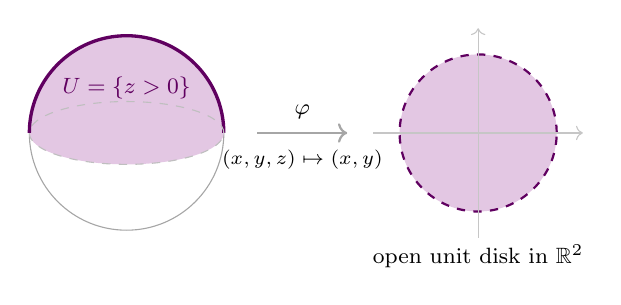
\begin{tikzpicture}[scale=0.95]
\draw[gray!70] (0,0) circle (1.3);
\fill[violet!22] (-1.3,0) arc (180:0:1.3) -- cycle;
\fill[violet!22] (0,0) ellipse (1.3 and 0.42);
\draw[violet!75!black,very thick] (-1.3,0) arc (180:0:1.3);
\draw[gray!50,dashed] (0,0) ellipse (1.3 and 0.42);
\node[violet!75!black,font=\footnotesize] at (0,0.6) {$U=\{z>0\}$};
\draw[->,thick,gray!70] (1.75,0) -- (2.95,0);
\node[font=\footnotesize,above] at (2.35,0.06) {$\varphi$};
\node[font=\scriptsize,below] at (2.35,-0.1) {$(x,y,z)\mapsto(x,y)$};
\begin{scope}[xshift=4.7cm]
\fill[violet!22] (0,0) circle (1.05);
\draw[violet!75!black,thick,dashed] (0,0) circle (1.05);
\draw[gray!45,->] (-1.4,0)--(1.4,0); \draw[gray!45,->] (0,-1.4)--(0,1.4);
\node[font=\footnotesize] at (0,-1.65) {open unit disk in $\mathbb{R}^2$};
\end{scope}
\end{tikzpicture}
\end{center}


\begin{propbox}[Spheres Are Topological Manifolds]\thmlabel{prop:sn-manifold}
$S^n = \{x \in \mathbb{R}^{n+1} \mid |x| = 1\}$ is a topological $n$-manifold.
\leeref{Example 1.4}
\end{propbox}

\begin{proof}
As in Example~\ref{ex:s2-manifold}, $S^n$ is a metric space (restriction of the Euclidean metric), hence Hausdorff, and second countable: intersecting a countable basis of $\mathbb{R}^{n+1}$ with $S^n$ gives a countable basis. The $2(n+1)$ open hemispheres $U_i^{\pm} = \{x \in S^n \mid \pm x_i > 0\}$ cover $S^n$, since every point has a nonzero coordinate. On $U_i^\pm$, the map $\varphi_i^\pm$ forgetting the $i$-th coordinate is continuous and lands in the open unit ball $B^n$, because the remaining coordinates satisfy $\sum_{j \ne i} x_j^2 = 1 - x_i^2 < 1$. Its inverse inserts $\pm\sqrt{1 - |y|^2}$ in slot $i$ and is continuous. So each $\varphi_i^\pm$ is a homeomorphism onto the open set $B^n \subseteq \mathbb{R}^n$, and Proposition~\ref{prop:open-charts} applies.
\end{proof}

\begin{rembox}\label{rem:manifolds-2}
This is the argument of Example~\ref{ex:s2-manifold}, for every $n$ (Lee, Example 1.4). The hemisphere charts will be our first example of an \emph{atlas}, and the maps between overlapping charts (\S\ref{sub:charts}) will turn out to be smooth.
\end{rembox}
\begin{exbox}[Two Hemisphere Charts on $S^2$]\exlabel{ex:two-hemisphere-charts-s2}
Take $U = \{z > 0\}$ with $\varphi(x, y, z) = (x, y)$ and $V = \{x > 0\}$ with $\psi(x, y, z) = (y, z)$, both charts onto the open unit disk. Then $U \cap V = \{x > 0, z > 0\}$, $\varphi(U \cap V) = \{(x, y) \in D \mid x > 0\}$, and
\[
\psi \circ \varphi^{-1}(x, y) = \psi\big(x, y, \sqrt{1 - x^2 - y^2}\big) = \big(y, \sqrt{1 - x^2 - y^2}\big).
\]
Note that this map is not merely continuous but $C^\infty$ on its (open) domain, since $1 - x^2 - y^2 > 0$ there. This is no accident, and it is the point of Definition~\ref{def:compatible}.
\end{exbox}
% ============================================================================
% SECTION: EXAMPLE: COMPLEX PROJECTIVE SPACE
% ============================================================================

\section{Complex Projective Space}\label{sec:ex-cpn}

\roadmark{Thread: quotients}{$\mathbb{CP}^n$, the first manifold built as a quotient: the open quotient $S^{2n+1}/S^1$ is Hausdorff, second countable (\ref{sec:open-quotients}) and compact, and it is the space of complex lines. Its charts come in \ref{sec:projective-smooth}.}

Complex projective space through the course: the open quotient $S^{2n+1}/S^1$, Hausdorff, second countable and compact, in Section~\ref{sec:ex-cpn}; the circle group $\Ugp(1)$ acting there in Example~\ref{ex:1-circle}; an orbit space in Example~\ref{ex:cpn-orbit}; a smooth and complex manifold through its standard atlas in Section~\ref{sec:projective-smooth}; a homogeneous space of $\Ugp(n+1)$ in Remark~\ref{rem:dimension-checks-through-homogeneous-spaces}; the domain of the moment map in Remark~\ref{rem:strategy}; and the base of the Hopf fibration in Section~\ref{sec:ex-hopf}.

\label{sub:cpn}
The following was set up in the last four minutes of lecture; the proof of the claim was given verbally, chalk down. \textbf{Uribe: ``I'll write this again next time''} --- so expect a careful reprise; the details below reconstruct the verbal argument.

\begin{defbox}[Complex Projective Space $\mathbb{CP}^n$]\deflabel{def:cpn}
Consider the sphere $S^{2n+1} \subseteq \mathbb{R}^{2n+2}$, and identify $\mathbb{R}^{2n+2} \cong \mathbb{C}^{n+1}$ by
\[
(x, y) \longmapsto x + iy, \qquad x, y \in \mathbb{R}^{n+1}
\]
(any such identification works). So points of $S^{2n+1}$ are complex vectors $z = (z_1, \dots, z_{n+1}) \in \mathbb{C}^{n+1}$ with $|z| = 1$. Let $S^1 = \{\xi \in \mathbb{C} \mid |\xi| = 1\}$ be the unit circle, and define a relation $\sim$ on $S^{2n+1}$ by
\[
z \sim w \iff \exists\, \xi \in S^1 \text{ such that } w = \xi z
\]
(componentwise complex multiplication: all entries of $w$ are obtained by rotating the entries of $z$ through the \emph{same} angle). This is an equivalence relation ($\xi = 1$ gives reflexivity; $\xi^{-1} \in S^1$ gives symmetry; products give transitivity). The quotient
\[
\mathbb{CP}^n \;:=\; S^{2n+1}/{\sim}
\]
is the \textbf{complex projective space} of complex dimension $n$. Explicitly: a point of $\mathbb{CP}^n$ is a class $[z] = \{\, \xi z \mid \xi \in S^1 \,\}$, a circle inside $S^{2n+1}$; $\pi(z) = [z]$; and $W \subseteq \mathbb{CP}^n$ is open iff the union of the circles belonging to $W$ is open in $S^{2n+1}$. The class $[z]$ is the same as the complex line $\mathbb{C} z \subseteq \mathbb{C}^{n+1}$ through $z$ (a line meets the unit sphere in exactly the circle $\{\xi z\}$), so $\mathbb{CP}^n$ is the space of complex lines through the origin in $\mathbb{C}^{n+1}$; the identification is $[z] \mapsto \mathbb{C} z$, with inverse $\ell \mapsto \ell \cap S^{2n+1}$.
\leeref{Problem 1-9}
\end{defbox}

\begin{propbox}[$\mathbb{CP}^n$ is Hausdorff and Second Countable]\thmlabel{prop:cpn}
The quotient topology on $\mathbb{CP}^n$ is $T_2$ and second countable.
\leeref{Problem 1-9}
\end{propbox}

\begin{proof}[Proof (verbal sketch in Lecture 2; the general form is Corollary~\ref{cor:orbit-T2})]
\textit{(Lecture~4: the graph of the orbit relation is the continuous image of the compact $G \times X$, hence compact, hence closed in the Hausdorff $X \times X$.)} We verify the two hypotheses of the Hausdorff Criterion.

\emph{The relation is open.} For $\xi \in S^1$ define $R_\xi : S^{2n+1} \to S^{2n+1}$, $R_\xi(z) = \xi z$. This is well defined: $|\xi z| = |\xi|\,|z| = |z| = 1$. It is continuous, being the restriction to $S^{2n+1}$ of the $\mathbb{C}$-linear (hence $\mathbb{R}$-linear, hence continuous) map $z \mapsto \xi z$ on $\mathbb{C}^{n+1} \cong \mathbb{R}^{2n+2}$. Since $\xi^{-1} \in S^1$ and $R_{\xi^{-1}} \circ R_\xi = R_\xi \circ R_{\xi^{-1}} = \mathrm{id}$, $R_\xi$ is a homeomorphism; in particular $R_\xi(U)$ is open for every open $U \subseteq S^{2n+1}$. Now let $U \subseteq S^{2n+1}$ be open. For $w \in S^{2n+1}$,
\begin{align*}
w \in \pi^{-1}(\pi(U)) &\iff \exists\, z \in U \text{ with } w \sim z \\
&\iff \exists\, z \in U,\ \xi \in S^1 \text{ with } w = \xi z \iff w \in \bigcup_{\xi \in S^1} R_\xi(U),
\end{align*}
so the saturation $\pi^{-1}(\pi(U)) = \bigcup_{\xi \in S^1} R_\xi(U)$ is a union of open sets, hence open. By Proposition~\ref{prop:saturation}, $\sim$ is open.

\emph{The graph is closed.} Define
\[
\Phi : S^1 \times S^{2n+1} \longrightarrow S^{2n+1} \times S^{2n+1}, \qquad \Phi(\xi, z) = (z, \xi z).
\]
By Theorem~\ref{thm:univ-product}, $\Phi$ is continuous because its two components are: $(\xi, z) \mapsto z$ is the projection, and $(\xi, z) \mapsto \xi z$ is the restriction of the map $\mathbb{C} \times \mathbb{C}^{n+1} \to \mathbb{C}^{n+1}$, $(\xi, z) \mapsto \xi z$, whose real and imaginary parts are polynomial in the real coordinates. Its image is $\Gamma$: for $(z, w) \in S^{2n+1} \times S^{2n+1}$,
\begin{align*}
(z, w) \in \Phi\big(S^1 \times S^{2n+1}\big) &\iff \exists\, \xi \in S^1 \text{ with } (z, w) = (z, \xi z) \\
&\iff \exists\, \xi \in S^1 \text{ with } w = \xi z \iff z \sim w \iff (z,w) \in \Gamma.
\end{align*}
$S^1 \subseteq \mathbb{R}^2$ and $S^{2n+1} \subseteq \mathbb{R}^{2n+2}$ are closed and bounded, hence compact, and a finite product of compact spaces is compact (Proposition~\ref{fact:compact}); so $S^1 \times S^{2n+1}$ is compact and its continuous image $\Gamma$ is compact. The space $S^{2n+1} \times S^{2n+1}$ is a subspace of $\mathbb{R}^{4n+4}$, hence metrizable, hence Hausdorff (Proposition~\ref{fact:metric}), and a compact subset of a Hausdorff space is closed (Proposition~\ref{fact:compact}). Therefore $\Gamma$ is closed in $S^{2n+1} \times S^{2n+1}$.

By the Hausdorff Criterion, $\mathbb{CP}^n$ is $T_2$; and since $S^{2n+1}$ is second countable (subspace of $\mathbb{R}^{2n+2}$) and $\sim$ is open, Theorem~\ref{thm:2c-quotient} gives second countability.
\end{proof}

\textbf{Transcription note.} Page~7 of the handwritten notes writes the map in this argument as $S^1 \times S^{2n+1} \to S^{2n+2} \times S^{2n+2}$; the target is $S^{2n+1} \times S^{2n+1}$, where the graph of the relation lives.

\textbf{Transcription note.} On the board (and in the handwritten notes) the target of $\Phi$ was written with superscripts $2n+2$; the target must be $S^{2n+1} \times S^{2n+1}$ --- pairs of points of the sphere being quotiented --- as recorded here.

\begin{proof}[A direct proof that $\mathbb{CP}^n$ is Hausdorff (Assignment 2)]
This bypasses the Hausdorff criterion and exhibits the separating sets. Let $u \neq v$ in $S^{2n+1}/S^1$, with representatives $\vec u, \vec v \in S^{2n+1}$. Their orbits $S^1 \vec u$ and $S^1 \vec v$ are disjoint (distinct orbits), and compact, being images of the compact $S^1$ under $\mu \mapsto \mu\vec u$, $\mu \mapsto \mu \vec v$.

\emph{The orbits are at positive distance.} Let $d = \inf\{|\vec a - \vec b| : \vec a \in S^1\vec u,\ \vec b \in S^1 \vec v\}$. If $d = 0$, choose $\vec a_k \in S^1\vec u$, $\vec b_k \in S^1\vec v$ with $|\vec a_k - \vec b_k| \to 0$; by compactness a subsequence $\vec a_{k_j} \to \vec a \in S^1\vec u$, whence $\vec b_{k_j} \to \vec a$ too, and $\vec a \in S^1 \vec v$ since that orbit is closed. This contradicts disjointness, so $d > 0$.

\emph{Thickened orbits.} Put $r = d/3$ and $A = \bigcup_{\lambda \in S^1} \lambda\, B(\vec u, r)$, $B = \bigcup_{\lambda \in S^1} \lambda\, B(\vec v, r)$, with balls taken in $S^{2n+1}$. Each is open (a union of images of an open set under the homeomorphisms $\vec z \mapsto \lambda\vec z$) and saturated (a union of orbits). If $\lambda\vec z_1 = \lambda'\vec z_2$ with $\vec z_1 \in B(\vec u, r)$, $\vec z_2 \in B(\vec v, r)$, then
\[
d \le |\lambda\vec u - \lambda'\vec v| \le |\lambda\vec u - \lambda \vec z_1| + |\lambda\vec z_1 - \lambda'\vec z_2| + |\lambda'\vec z_2 - \lambda'\vec v| < r + 0 + r = \tfrac23 d,
\]
using $|\lambda| = |\lambda'| = 1$; a contradiction, so $A \cap B = \emptyset$. Since $\pi$ is open and $A$, $B$ are disjoint and saturated, $\pi(A)$ and $\pi(B)$ are disjoint open neighbourhoods of $u$ and $v$.
\end{proof}

\begin{rembox}\label{rem:new-spaces-6}
The one place the group enters the direct proof is $|\lambda \vec u - \lambda \vec z_1| = |\vec u - \vec z_1|$: every $\lambda \in S^1$ is an \emph{isometry}, so the thickening by $r$ is uniform over the whole group. That uniformity --- a compact group acting by isometries --- is the concrete mechanism behind Corollary~\ref{cor:orbit-T2}, and it is exactly what fails for $\mathbb{R}^+$ in Example~\ref{ex:nonhausdorff-orbit}, where $t \cdot (x,y) = (tx, y/t)$ distorts distances without bound.
\end{rembox}

\begin{propbox}[$\mathbb{CP}^n$ Is Compact]\thmlabel{prop:cpn-compact}
$\mathbb{CP}^n$ is compact.
\leeref{Problem 1-9}
\end{propbox}

\begin{proof}
\textit{(Not from lecture; filled in.)} $S^{2n+1} \subseteq \mathbb{R}^{2n+2}$ is closed and bounded, hence compact (Proposition~\ref{fact:compact}(1)), and $\mathbb{CP}^n = \pi(S^{2n+1})$ is its image under the continuous surjection $\pi$.
\end{proof}

\begin{propbox}[$\mathbb{CP}^n$ as the Space of Complex Lines]\thmlabel{prop:cpn-lines}
Let the multiplicative group $\mathbb{C}^\times = \mathbb{C} \setminus \{0\}$ act on $\mathbb{C}^{n+1} \setminus \{0\}$ by scalar multiplication, $\lambda \cdot \vec z = \lambda \vec z$. Then:
\begin{enumerate}
    \item this is a continuous action, and the orbit of $\vec z$ is the punctured complex line $\operatorname{span}_{\mathbb{C}}(\vec z) \setminus \{0\}$; so the orbit space $(\mathbb{C}^{n+1} \setminus \{0\})/\mathbb{C}^\times$ is in natural bijection with the set of complex lines through the origin in $\mathbb{C}^{n+1}$;
    \item the map
    \[
    \Theta : \big(\mathbb{C}^{n+1} \setminus \{0\}\big)/\mathbb{C}^\times \longrightarrow S^{2n+1}/S^1, \qquad \mathbb{C}^\times\vec z \longmapsto S^1 \cdot \frac{\vec z}{|\vec z|},
    \]
    is a homeomorphism.
\end{enumerate}
Consequently the two natural quotient topologies on the set of lines agree, and either may be taken as the topology of $\mathbb{CP}^n$.
\leeref{Problem 1-9}
\end{propbox}

\begin{center}
\begin{tikzcd}[row sep=3.2em, column sep=4.6em]
\mathbb{C}^{n+1}\setminus\{0\} \arrow[r, shift left=0.8ex, "g"] \arrow[d, "\pi_1"'] & S^{2n+1} \arrow[l, shift left=0.8ex, hook', "\iota"] \arrow[d, "\pi_2"] \\
\big(\mathbb{C}^{n+1}\setminus\{0\}\big)/\mathbb{C}^\times \arrow[r, shift left=0.8ex, "\Theta"] & S^{2n+1}/S^1 \arrow[l, shift left=0.8ex, "\Psi"]
\end{tikzcd}
\end{center}

Here $g(\vec z) = \vec z/|\vec z|$ and $\iota$ is the inclusion. Both squares commute: $\Theta \circ \pi_1 = \pi_2 \circ g$ and $\Psi \circ \pi_2 = \pi_1 \circ \iota$. Upstairs, $g$ and $\iota$ are \emph{not} mutually inverse --- $g \circ \iota = \mathrm{id}$, but $\iota \circ g$ replaces $\vec z$ by $\vec z/|\vec z|$. Downstairs they become inverse, because passing to the quotient forgets exactly the scale that $\iota \circ g$ changes. The proof below is the chase around these two squares.


\begin{proof}
Write $\pi_1 : \mathbb{C}^{n+1}\setminus\{0\} \to (\mathbb{C}^{n+1}\setminus\{0\})/\mathbb{C}^\times$ and $\pi_2 : S^{2n+1} \to S^{2n+1}/S^1$ for the two projections, both quotient maps.

(1) If $\lambda \neq 0$ and $\vec z \neq 0$ then $\lambda\vec z \neq 0$, so the action preserves $\mathbb{C}^{n+1}\setminus\{0\}$. The axioms are $1 \cdot \vec z = \vec z$ and associativity of multiplication in $\mathbb{C}$, coordinatewise. Continuity: each component $(\lambda, \vec z) \mapsto \lambda z_k$ is polynomial in the real and imaginary parts (Definition~\ref{def:complex-groups}), and the action is the restriction of this map to a subspace. The orbit $\{\lambda\vec z : \lambda \neq 0\}$ is $\operatorname{span}_{\mathbb{C}}(\vec z) \setminus \{0\}$, and a line $\ell$ is recovered from $\ell \setminus \{0\}$ by adjoining $0$.

(2) \emph{$\Theta$ is well defined and continuous.} Let $g(\vec z) = \vec z/|\vec z|$, continuous on $\mathbb{C}^{n+1} \setminus \{0\}$ with values in $S^{2n+1}$. For $\lambda \in \mathbb{C}^\times$,
\[
g(\lambda\vec z) = \frac{\lambda}{|\lambda|}\, g(\vec z), \qquad \Big|\frac{\lambda}{|\lambda|}\Big| = 1,
\]
so $g(\lambda\vec z)$ and $g(\vec z)$ lie in the same $S^1$-orbit: $\pi_2 \circ g$ is constant on the fibres of $\pi_1$, although $g$ itself is not. By the universal property (Theorem~\ref{thm:univ-quotient-full}), $\pi_2 \circ g$ descends to a unique continuous map on the $\mathbb{C}^\times$-quotient, which is $\Theta$.

\emph{The inverse is continuous.} Let $\iota : S^{2n+1} \hookrightarrow \mathbb{C}^{n+1}\setminus\{0\}$ be the inclusion. Then $\pi_1 \circ \iota$ is continuous and constant on $S^1$-orbits, since $S^1 \subseteq \mathbb{C}^\times$; so it descends to a continuous $\Psi : S^{2n+1}/S^1 \to (\mathbb{C}^{n+1}\setminus\{0\})/\mathbb{C}^\times$, $S^1\vec z \mapsto \mathbb{C}^\times \vec z$.

\emph{They are mutually inverse.} For $|\vec z| = 1$, $\Theta(\Psi(S^1\vec z)) = S^1 \vec z$; for $\vec z \neq 0$, $\Psi(\Theta(\mathbb{C}^\times\vec z)) = \mathbb{C}^\times(\vec z/|\vec z|) = \mathbb{C}^\times\vec z$, the vector $\vec z/|\vec z|$ lying in the $\mathbb{C}^\times$-orbit of $\vec z$.
\end{proof}

\begin{rembox}\label{rem:new-spaces-7}
The key identity behind (2) is that for a unit vector $\vec z$ the part of its $\mathbb{C}^\times$-orbit lying on the sphere is exactly its $S^1$-orbit: $|\lambda\vec z| = |\lambda|$, which equals $1$ iff $\lambda \in S^1$. So each punctured line meets the unit sphere in precisely one circle, and normalizing $\vec z \mapsto \vec z/|\vec z|$ is the bridge between the two descriptions --- a point downstairs, a whole line upstairs in one, a circle upstairs in the other.
\end{rembox}

\begin{exbox}[Why the Origin Must Be Removed]\exlabel{ex:cpn-origin}
Let $\mathbb{C}^\times$ act instead on all of $\mathbb{C}^{n+1}$ by scalar multiplication. The action is still continuous, but the orbit space acquires one extra point, the orbit $\{\lambda \cdot 0\} = \{0\}$, which is not a line; and that point cannot be separated from any other. Indeed, let $U$ be an open set of the quotient containing $\{0\}$. Its preimage is open, saturated, and contains $0$, hence contains a ball $B(0,\varepsilon)$. For every $\vec z \neq 0$ the vector $\frac{\varepsilon}{2|\vec z|}\vec z$ lies in that ball and in the orbit of $\vec z$, so by saturation the preimage contains every orbit. Thus $U$ is the whole quotient: every neighbourhood of $\{0\}$ contains every point, and the quotient is not Hausdorff. Deleting the origin removes exactly this one orbit. Every orbit accumulates at $0$ --- the same pathology as Example~\ref{ex:nonhausdorff-orbit}, where orbits accumulate on other orbits, here concentrated at a single point.
\end{exbox}

\begin{rembox}[Where This Is Going]\label{rem:where-this-going}
$\mathbb{CP}^n$ is ``one of the main examples of manifolds'' and will recur throughout the course. With $T_2$ and second countability now secured, what is missing from manifold status is the locally Euclidean condition --- charts on $\mathbb{CP}^n$ --- which is supplied in \S\ref{sub:projective-atlas}, together with the smooth structure. The same two-step pattern ($\sim$ open via a group acting by homeomorphisms + graph closed via compactness) is the template for many quotient constructions to come: real projective space $\mathbb{RP}^n$ (Lee Example 1.5), Grassmannians, tori, and lens spaces all fit it.
\end{rembox}
\chapter{Topological Groups and Homogeneous Spaces}

% ============================================================================
% Lecture 3 (Fri Sep 4, 2026), first part
% SECTION 5: TOPOLOGICAL GROUPS AND CLASSICAL MATRIX GROUPS
% ============================================================================
\section{Topological Groups and Classical Matrix Groups}\label{sec:topgroups}

\roadmark{Thread: equations}{Topological groups and the classical matrix groups. That the classical groups are manifolds, as level sets of polynomial maps (\ref{sec:rvt}), is \ref{sec:classical-manifolds}; acting on spaces, they then feed the quotient thread.}

\textit{Reference: Lee Ch.\ 7 (``Lie Groups''). For the calculus: MATH 452 notes (Implicit Function Theorem).}

\begin{rembox}[Why This Section]\label{rem:why-this-section-3}
Topological groups are the precursor of \emph{Lie groups}, one of the main topics later in the course; and the classical matrix groups introduced here ``are going to be our friends for the semester, and hopefully for later on in life.'' Besides being examples of manifolds in their own right (\S\ref{sub:classical-manifolds}), they are the groups whose \emph{actions} produce the quotient manifolds of \ref{sec:actions}--\ref{sec:homogeneous}: spheres, projective spaces, Grassmannians.
\end{rembox}

\subsection{Topological Groups}

\begin{defbox}[Topological Group]\deflabel{def:top-group}
A \textbf{topological group} is a group $G$ equipped with a topology such that the two structures are compatible, meaning that both maps
\begin{enumerate}
    \item $G \times G \to G$, $(g, h) \mapsto gh$ \quad (multiplication), and
    \item $G \to G$, $g \mapsto g^{-1}$ \quad (inversion)
\end{enumerate}
are continuous, where $G \times G$ carries the product topology.
\leeref{Ch.~7, p.~151 (defined in passing)}
\end{defbox}

\begin{exbox}[Discrete Groups]\exlabel{ex:discrete-groups}
Any group $G$ with the discrete topology is a topological group: every subset is open, so every map out of $G$ or $G \times G$ (which is also discrete) is continuous. Uribe: mathematically immediate, but it ``actually shows up in useful ways.''
\end{exbox}

\begin{propbox}[Subgroups Are Topological Groups]\thmlabel{prop:subgroup-topgroup}
If $G$ is a topological group and $H \le G$ is a subgroup, then $H$ with the subspace topology is a topological group.
\leeref{cf.\ Ch.~7, \emph{Lie Subgroups}}
\end{propbox}

\begin{proof}
\textit{(Not from lecture; filled in.)} The multiplication of $H$ is the composite $H \times H \hookrightarrow G \times G \to G$, where the first map is $\iota \times \iota$ (continuous by Theorem~\ref{thm:univ-product}, since each component is $\iota \circ \pi$) and the second is the multiplication of $G$. This composite is continuous and takes values in $H$, so it is continuous as a map into $H$ by Proposition~\ref{prop:univ-subspace}. Inversion on $H$ is the restriction of inversion on $G$, and the same argument applies.
\end{proof}

\subsection{Classical Matrix Groups}

\begin{defbox}[Matrices as a Euclidean Space]\deflabel{def:mat-euclid}
Let $\Mat(n, \mathbb{R})$ be the set of all $n \times n$ real matrices, a real vector space under entrywise addition and scalar multiplication. For $1 \le i, j \le n$ let $E_{ij} \in \Mat(n,\mathbb{R})$ be the matrix with a $1$ in position $(i,j)$ and $0$ elsewhere. Every $g$ can be written uniquely as $g = \sum_{i,j} g_{ij} E_{ij}$, so $\{E_{ij}\}$ is a basis and $\dim \Mat(n,\mathbb{R}) = n^2$. Fix the coordinate map
\[
\Mat(n,\mathbb{R}) \longrightarrow \mathbb{R}^{n^2}, \qquad g \longmapsto (g_{11}, g_{12}, \ldots, g_{1n},\ g_{21}, \ldots, g_{2n},\ \ldots,\ g_{n1}, \ldots, g_{nn}),
\]
which reads the entries row by row (entry $(i,j)$ goes to coordinate number $n(i-1) + j$). This is a linear isomorphism, and we \textbf{define} the topology on $\Mat(n,\mathbb{R})$ by declaring it a homeomorphism onto $\mathbb{R}^{n^2}$ with the usual topology. Every subset of $\Mat(n,\mathbb{R})$ then carries the subspace topology. Concretely, a sequence of matrices converges iff each of its $n^2$ entries converges, and the Euclidean norm on $\mathbb{R}^{n^2}$ pulls back to $\|g\| = \big(\sum_{i,j} g_{ij}^2\big)^{1/2}$.
\leeref{Example 1.25}
\end{defbox}

\begin{defbox}[Permutations and the Sign]\deflabel{def:sgn}
The \textbf{symmetric group} $S_n$ is the set of all bijections $\sigma : \{1, \ldots, n\} \to \{1, \ldots, n\}$, a group under composition, of order $n!$. A \textbf{transposition} is a permutation that swaps two symbols and fixes the rest. An \textbf{inversion} of $\sigma$ is a pair $i < j$ with $\sigma(i) > \sigma(j)$. The \textbf{sign} of $\sigma$ is
\[
\sgn(\sigma) = (-1)^{\#\{\text{inversions of } \sigma\}} \in \{\pm 1\}.
\]
\leeref{App.~B, \emph{The Determinant}}
\end{defbox}

\begin{propbox}[Properties of the Sign]\thmlabel{prop:sgn}
\begin{enumerate}
    \item $\sgn : S_n \to \{\pm 1\}$ is a group homomorphism: $\sgn(\sigma\tau) = \sgn(\sigma)\sgn(\tau)$.
    \item Every transposition has sign $-1$, and $\sgn(\mathrm{id}) = 1$.
    \item Every $\sigma \in S_n$ is a product of transpositions; the number of factors is not unique, but its parity is, and $\sgn(\sigma) = (-1)^k$ for any factorization of $\sigma$ into $k$ transpositions.
    \item If $\sigma$ fixes $n - 1$ of the $n$ symbols, then $\sigma = \mathrm{id}$.
\end{enumerate}
\leeref{App.~B, \emph{The Determinant}}
\end{propbox}

\begin{proof}
(4) is elementary: if $\sigma(i) = i$ for all $i \neq j$, then $\sigma(j)$ must be the one remaining value $j$, since $\sigma$ is injective. (1)--(3) are proved in MATH 493 (Dummit--Foote \S3.5); the standard route is to let $\sigma$ act on the polynomial $\Delta = \prod_{i<j}(x_i - x_j)$ by permuting variables, observe that $\sigma \cdot \Delta = \sgn(\sigma)\,\Delta$ with $\sgn$ as in Definition~\ref{def:sgn}, and read off (1) from the fact that this is a group action; (2) is a direct count; (3) follows from (1) and (2) once one knows transpositions generate $S_n$.
\end{proof}

\begin{exbox}[Small Cases: Two and Three]\exlabel{ex:small-cases-two-three}
$S_2 = \{\mathrm{id}, (1\,2)\}$ with signs $+1, -1$, and the Leibniz formula below reads $\det = x_{11}x_{22} - x_{12}x_{21}$. $S_3$ has six elements: the identity and the two $3$-cycles $(1\,2\,3)$, $(1\,3\,2)$ have sign $+1$ (each $3$-cycle is a product of two transpositions, e.g.\ $(1\,2\,3) = (1\,3)(1\,2)$), and the three transpositions $(1\,2)$, $(1\,3)$, $(2\,3)$ have sign $-1$; this is the six-term formula for a $3 \times 3$ determinant, with three plus and three minus signs.
\end{exbox}

\begin{rembox}\label{rem:topgroups}
The facts used in the determinant computation of Proposition~\ref{prop:jacobi} are exactly (2) and (4) above: the identity permutation contributes with sign $+1$ (which is why the answer is $+\tr V$), and a permutation fixing all but one symbol is the identity (which is why only that one term survives).
\end{rembox}

\begin{propbox}[Determinant Is Continuous]\thmlabel{prop:det-cont}
$\det : \Mat(n,\mathbb{R}) \to \mathbb{R}$ is continuous.
\leeref{App.~B, \emph{The Determinant}}
\end{propbox}

\begin{proof}
\textit{(Implicit in Lecture~3, which used that $\GL(n,\mathbb{R}) = \det^{-1}(\mathbb{R} \setminus \{0\})$ is open; filled in.)} By the Leibniz formula $\det(x) = \sum_{\sigma \in S_n} \sgn(\sigma) \prod_{i=1}^n x_{i,\sigma(i)}$ (with $S_n$ and $\sgn$ as in Definition~\ref{def:sgn}; each $\sigma$ selects one entry from every row, $x_{i,\sigma(i)}$ from row $i$, and bijectivity of $\sigma$ means every column is used exactly once), $\det$ is a polynomial in the $n^2$ coordinates, and polynomials are continuous.
\end{proof}

\begin{defbox}[General Linear Group]\deflabel{def:GL}
The \textbf{general linear group} is
\[
\GL(n, \mathbb{R}) = \det{}^{-1}\big(\mathbb{R} \setminus \{0\}\big) = \{\, g \in \Mat(n,\mathbb{R}) \mid g \text{ is invertible} \,\},
\]
with the subspace topology. Being the preimage of an open set under a continuous map, it is an \textbf{open subset} of $\Mat(n,\mathbb{R}) \cong \mathbb{R}^{n^2}$.
\leeref{Example 1.27}
\end{defbox}

\begin{propbox}[$\GL({n,\mathbb{R}})$ Is a Topological Group]\thmlabel{prop:GL-topgroup}
$\GL(n,\mathbb{R})$ with the subspace topology is a topological group.
\leeref{Examples 1.27 and 7.3}
\end{propbox}

\begin{proof}
\textit{(Lecture~3: the formulas are algebraic --- the product in the coordinates, the inverse ``using cofactors and determinants'' --- ``so one and two are algebraic maps, hence continuous.'' The details are filled in below.)} Multiplication: $(gh)_{ik} = \sum_j g_{ij} h_{jk}$ is a polynomial in the entries of $(g,h) \in \mathbb{R}^{n^2} \times \mathbb{R}^{n^2} = \mathbb{R}^{2n^2}$, so $\Mat \times \Mat \to \Mat$ is continuous; its restriction to $\GL \times \GL$ (subspace of the product, which is the product of the subspaces) is continuous and lands in $\GL$, hence is continuous into $\GL$ by Proposition~\ref{prop:univ-subspace}. Inversion: by the cofactor formula, $g^{-1} = \adj(g)/\det(g)$, where each entry of the adjugate $\adj(g)$ is a polynomial in the entries of $g$ and $\det(g) \neq 0$ on $\GL$; so each entry of $g^{-1}$ is a rational function with nonvanishing denominator, hence continuous on $\GL$. Uribe's summary: ``one and two are algebraic maps, hence continuous.''
\end{proof}

The disconnectedness of $\GL(n,\mathbb{R})$ and of $\Ogp(n)$, why $\SO(n)$ is a proper subgroup of $\Ogp(n)$, and $\Ugp(1) = S^1$ are collected in Section~\ref{sec:ex-classical}.

\begin{defbox}[Special Linear Group]\deflabel{def:special-linear-group}
$\SL(n,\mathbb{R}) = \det^{-1}(1) \subseteq \GL(n,\mathbb{R})$, the matrices of determinant $1$. It is a subgroup ($\det$ is multiplicative), hence a topological group with the subspace topology (Proposition~\ref{prop:subgroup-topgroup}), and it is closed in $\Mat(n,\mathbb{R})$ (preimage of the closed set $\{1\}$).
\end{defbox}

\begin{defbox}[Orthogonal Group]\deflabel{def:orthogonal-group}
The \textbf{orthogonal group} is
\[
\Ogp(n,\mathbb{R}) = \{\, g \in \GL(n,\mathbb{R}) \mid (gx) \cdot (gy) = x \cdot y \ \text{ for all } x, y \in \mathbb{R}^n \,\},
\]
the linear maps preserving the dot product.
\end{defbox}

\begin{propbox}[Equivalent Description of $\Ogp({n,\mathbb{R}})$]\thmlabel{prop:orth-equiv}
For $g \in \GL(n,\mathbb{R})$ the following are equivalent: (i) $g \in \Ogp(n,\mathbb{R})$; (ii) $g^T g = I$; (iii) $g^{-1} = g^T$. Consequently $\det(g)^2 = 1$, i.e.\ $\det g = \pm 1$, for every $g \in \Ogp(n,\mathbb{R})$.
\leeref{Example 7.27}
\end{propbox}

\begin{proof}
\textit{(Stated in Lecture~3 --- ``$g \in \Ogp(n) \iff g^{-1} = g^{\mathsf T}$''; filled in.)} Writing the dot product as $x \cdot y = x^T y$, we have $(gx)\cdot(gy) = x^T g^T g\, y$. If $g^T g = I$ this equals $x^T y$, so (ii) $\Rightarrow$ (i). Conversely, if (i) holds, take $x = e_i$, $y = e_j$: then $(g^T g)_{ij} = e_i^T g^T g\, e_j = e_i \cdot e_j = \delta_{ij}$, so $g^T g = I$. (ii) $\iff$ (iii) since for square matrices a one-sided inverse is two-sided. Finally $1 = \det(I) = \det(g^T g) = \det(g^T)\det(g) = \det(g)^2$.
\end{proof}
\begin{defbox}[Special Orthogonal Group]\deflabel{def:special-orthogonal-group}
$\SO(n,\mathbb{R}) = \Ogp(n,\mathbb{R}) \cap \SL(n,\mathbb{R}) = \{\, g \in \Ogp(n,\mathbb{R}) \mid \det g = 1 \,\}$.
\end{defbox}

\begin{defbox}[Complex Matrix Groups]\deflabel{def:complex-groups}
Once and for all, fix the $\mathbb{R}$-linear identification $\mathbb{C} \cong \mathbb{R}^2$, $x + iy \mapsto (x, y)$, and hence $\mathbb{C}^n \cong \mathbb{R}^{2n}$: explicitly, writing $z_j = x_j + i y_j$,
\[
(z_1, \ldots, z_n) \longmapsto (x_1, y_1, x_2, y_2, \ldots, x_n, y_n).
\]
(Any other ordering of the real coordinates, e.g.\ all $x$'s first, differs by a linear homeomorphism and changes nothing topologically; the choice made in \S\ref{sub:cpn} was of the latter kind.) Applying this to each entry of a complex matrix, in the row-by-row order of Definition~\ref{def:mat-euclid}, gives the coordinate map
\[
\Mat(n,\mathbb{C}) \longrightarrow \mathbb{R}^{2n^2}, \qquad g \longmapsto \big(\operatorname{Re} g_{11}, \operatorname{Im} g_{11},\ \operatorname{Re} g_{12}, \operatorname{Im} g_{12},\ \ldots,\ \operatorname{Re} g_{nn}, \operatorname{Im} g_{nn}\big),
\]
which defines the topology on $\Mat(n,\mathbb{C})$. Then $\det : \Mat(n,\mathbb{C}) \to \mathbb{C} \cong \mathbb{R}^2$ is continuous (its real and imaginary parts are polynomials in these $2n^2$ real coordinates, since $\det$ is a polynomial in the complex entries), and
\[
\GL(n,\mathbb{C}) = \det{}^{-1}(\mathbb{C} \setminus \{0\}) = \{\text{invertible complex } n \times n \text{ matrices}\}
\]
is open in $\Mat(n,\mathbb{C})$ and is a topological group by the same algebraic argument as over $\mathbb{R}$. The \textbf{unitary group} is
\[
\Ugp(n) = \{\, g \in \GL(n,\mathbb{C}) \mid g^{-1} = \bar{g}^{\,T} \,\},
\]
where $\bar g$ is the entrywise complex conjugate; $\bar g^{\,T}$ is also written $g^\dagger$ or $g^*$. It is the analogue of $\Ogp(n)$ with the dot product replaced by the Hermitian inner product $\langle z, w \rangle = \sum_j z_j \bar w_j$: $g \in \Ugp(n)$ iff $\langle gz, gw \rangle = \langle z, w \rangle$ for all $z, w$ (same proof as Proposition~\ref{prop:orth-equiv}, with $e_i^T \bar{g}^{\,T} g\, e_j$ in place of $e_i^T g^T g\, e_j$).
\leeref{Examples 7.29 and 7.30}
\end{defbox}

\begin{exbox}[$\Ugp(1)$ Is the Circle]\exlabel{ex:1-circle}
A $1 \times 1$ complex matrix is a number $\xi \in \mathbb{C}$, all such matrices are symmetric, and the condition $\xi^{-1} = \bar\xi$ reads $\xi \bar\xi = |\xi|^2 = 1$. So
\[
\Ugp(1) = \{\, \xi \in \mathbb{C} \setminus \{0\} \mid |\xi| = 1 \,\} = S^1,
\]
the unit circle, which is the notation ``everybody uses.'' This is the group acting in the construction of $\mathbb{CP}^n$ (\S\ref{sub:cpn}).
\end{exbox}

% ============================================================================
% SECTION: THE CLASSICAL GROUPS ARE TOPOLOGICAL MANIFOLDS
% ============================================================================

\section{The Classical Groups Are Topological Manifolds}\label{sec:classical-manifolds}\label{sub:classical-manifolds}

\roadmark{Thread: equations}{The classical groups as regular level sets of polynomial maps (\ref{sec:rvt}): each is a topological manifold.}

\begin{rembox}[The Method: Level Sets and the Implicit Function Theorem]\label{rem:method-level-sets-implicit-function-theorem}
``For the first time, we're going to use some calculus.'' $\SL(n,\mathbb{R})$ is a \emph{level set}, $\det^{-1}(1)$, of a smooth function on $\mathbb{R}^{n^2}$. Multivariable calculus says that a level set of $F$ is locally a graph---hence locally Euclidean---near any point where $\nabla F \neq 0$. So the work is to compute $\nabla \det$ and show it does not vanish on $\SL(n,\mathbb{R})$. Uribe's methodological message: the Leibniz formula makes computing $\nabla\det$ directly ``a nightmare''; instead, \emph{differentiate along curves} and use the chain rule. ``It's nice to compute gradients or differentials using curves.'' This kind of computation ``will happen several times.''
\end{rembox}

Throughout, identify $\Mat(n,\mathbb{R}) = \mathbb{R}^{n^2}$ via Definition~\ref{def:mat-euclid}, writing $x_{ij}$ for the coordinate that reads off the $(i,j)$ entry, and for $F : \mathbb{R}^{n^2} \to \mathbb{R}$ differentiable write $\nabla F(g) \in \mathbb{R}^{n^2}$ for the gradient, with components $\partial F/\partial x_{ij}(g)$. The dot product on $\mathbb{R}^{n^2}$ is $A \cdot B = \sum_{i,j} A_{ij} B_{ij}$. The chain rule for a curve $\gamma$ reads $\frac{d}{dt} F(\gamma(t)) = \nabla F(\gamma(t)) \cdot \gamma'(t)$.

\begin{propbox}[Derivative of the Determinant]\thmlabel{prop:jacobi}
Let $g \in \GL(n,\mathbb{R})$ and $A \in \Mat(n,\mathbb{R})$. Then
\[
\nabla \det(g) \cdot A \;=\; \frac{d}{dt}\Big|_{t=0} \det(g + tA) \;=\; \det(g)\, \tr\!\big(g^{-1} A\big).
\]
In particular, for $g \in \SL(n,\mathbb{R})$: $\nabla\det(g) \cdot A = \tr(g^{-1}A)$.
\leeref{Problem 7-4}
\end{propbox}

\begin{proof}
\textit{(Lecture~3's computation, as on the board --- page~9 of the handwritten notes. A student caught the order of operations: differentiate first, then set $t = 0$.)} The first equality is the chain rule applied to the affine line $\gamma(t) = g + tA$, for which $\gamma(0) = g$ and $\gamma'(t) = A$.

For the second, factor out $g$ (invertible): $g + tA = g\,(I + t g^{-1} A)$. Put $V = g^{-1}A$. Since $\det$ is multiplicative,
\[
\det(g + tA) = \det(g)\, \det(I + tV),
\]
and $\det(g)$ is a constant, so it suffices to show $\frac{d}{dt}\big|_{t=0} \det(I + tV) = \tr V$. By the Leibniz formula, with $(I + tV)_{ij} = \delta_{ij} + t V_{ij}$,
\[
\det(I + tV) = \sum_{\sigma \in S_n} \sgn(\sigma) \prod_{i=1}^n \big( \delta_{i,\sigma(i)} + t\, V_{i,\sigma(i)} \big).
\]
Differentiation is linear, so it passes inside the finite sum. For the product of $n$ factors use the product rule in the form $\frac{d}{dt} \prod_{i=1}^n f_i(t) = \sum_{j=1}^n f_j'(t) \prod_{i \neq j} f_i(t)$; here $f_i(t) = \delta_{i,\sigma(i)} + t V_{i,\sigma(i)}$, so $f_j'(t) = V_{j,\sigma(j)}$. Differentiating first and only then setting $t = 0$ (in the other order one gets $0$),
\[
\frac{d}{dt}\Big|_{t=0} \det(I + tV) = \sum_{\sigma \in S_n} \sgn(\sigma) \sum_{j=1}^n V_{j,\sigma(j)} \prod_{i \neq j} \delta_{i,\sigma(i)}.
\]
Fix $\sigma$ and $j$. The product $\prod_{i \neq j} \delta_{i,\sigma(i)}$ is nonzero only if $\sigma(i) = i$ for all $i \neq j$; a permutation fixing $n-1$ of the $n$ symbols is the identity (Proposition~\ref{prop:sgn}(4)), so $\sigma = \mathrm{id}$, for which $\sgn(\sigma) = 1$ and the product equals $1$. Every other permutation contributes $0$. Hence
\[
\frac{d}{dt}\Big|_{t=0} \det(I + tV) = \sum_{j=1}^n V_{jj} = \tr V = \tr(g^{-1}A). \qedhere
\]
\end{proof}

In lecture the computation was carried out for $g \in \SL(n,\mathbb{R})$, where $\det(g) = 1$ and the factor disappears; the general-$g$ statement (Jacobi's formula) is the same computation with the constant $\det(g)$ carried along.

\begin{corbox}[Jacobi's Formula --- Gradient Form]\thmlabel{cor:jacobi-gradient}
For invertible $g$,
\[
\nabla\det(g) = \det(g)\,(g^{-1})^{\mathsf T}
\]
as an element of $\mathbb{R}^{n^2}$ arranged as an $n \times n$ matrix; equivalently $\dfrac{\partial \det}{\partial x_{ij}}(g) = \adj(g)_{ji}$, the $(i,j)$ cofactor of $g$.
\leeref{Problem 7-4}
\end{corbox}

\begin{proof}
$\det$ is scalar-valued, so its gradient at $g$ is a vector in $\mathbb{R}^{n^2}$, determined by its dot products with all directions $A$, and Proposition~\ref{prop:jacobi} gives those dot products as $\det(g)\tr(g^{-1}A)$. Expanding the trace,
\[
\tr(g^{-1}A) = \sum_{i,j} (g^{-1})_{ji}\, A_{ij} = \sum_{i,j} \big((g^{-1})^{\mathsf T}\big)_{ij}\, A_{ij} = (g^{-1})^{\mathsf T} \cdot A .
\]
As this holds for every $A$, $\nabla\det(g) = \det(g)(g^{-1})^{\mathsf T}$. By the cofactor formula $g^{-1} = \adj(g)/\det(g)$ this is $\adj(g)^{\mathsf T}$, whose $(i,j)$ entry is $\adj(g)_{ji}$.
\end{proof}

\begin{rembox}[The Gradient Itself]\label{rem:gradient-itself}
Differentiating the determinant with respect to one entry recovers the cofactor expansion along that entry's row. The directional form of Proposition~\ref{prop:jacobi} is the one used in proofs; the gradient form is what one checks against a direct computation for $n = 2$.
\end{rembox}

\begin{corbox}[$1$ Is a Regular Value of $\det$]\thmlabel{cor:regular-value}
For every $g \in \SL(n,\mathbb{R})$, $\nabla \det(g) \neq 0$. Hence every point of the level set $\det^{-1}(1)$ is a regular point of $\det$, i.e.\ $1$ is a regular value of $\det$ (Definition~\ref{def:regular-value}). Equivalently, $0$ is a regular value of the function $\det - 1$, which has the same gradient and the same level set $\{\det - 1 = 0\}$.
\leeref{Ch.~7, p.~158}
\end{corbox}

\begin{proof}
\textit{(Lecture~3: ``I can easily find matrices $A$ for which this is not zero, so the gradient cannot be zero''; the choice $A = g$ is filled in.)} Take $A = g$ in Proposition~\ref{prop:jacobi}: $\nabla\det(g) \cdot g = \tr(g^{-1} g) = \tr(I) = n \neq 0$. A vector with a nonzero dot product against something is nonzero.
\end{proof}

\textbf{Transcription note.} Both the board and the audio say ``$0 \in \mathbb{R}$ is a regular value of $\det$.'' Read literally this is false for $n \ge 2$: the zero matrix lies in $\det^{-1}(0)$, and along the line $\gamma(t) = tA$ one has $\det(tA) = t^n \det A$, whose derivative at $t = 0$ vanishes for $n \ge 2$; so $\nabla\det(0) = 0$ and $0$ is a critical value. What the computation proves is that $1$ is a regular value of $\det$ (or $0$ of $\det - 1$, the form in which level sets are usually written as zero sets). The general statement is Corollary~\ref{cor:det-regular} below.

\begin{corbox}[Every Nonzero Value Is a Regular Value of $\det$]\thmlabel{cor:det-regular}
Every $c \ne 0$ is a regular value of $\det : \Mat(n,\mathbb{R}) \to \mathbb{R}$, so $\det^{-1}(c)$ is a topological manifold of dimension $n^2 - 1$. For $c = 1$ this is $\SL(n,\mathbb{R})$, treated in Corollary~\ref{prop:SL-loc-euc} below.
\leeref{Ch.~7, p.~158}
\end{corbox}

\begin{proof}
\textit{(Not from lecture: the general form of Corollary~\ref{cor:regular-value}.)} Let $\det g = c \ne 0$. By Proposition~\ref{prop:jacobi} in the direction $A = g$,
\[
\nabla\det(g) \cdot g = \det(g)\,\tr(g^{-1}g) = c\,n \ne 0,
\]
so $\nabla\det(g) \ne 0$ and $D\det_g$ is onto $\mathbb{R}$. Theorem~\ref{thm:regular-value} gives the manifold.
\end{proof}

The passage from ``nonvanishing gradient'' to ``locally a graph'' is the Implicit Function Theorem, proved in MATH 452 and used here as a black box. We record it in the general vector-valued form, since that is what the regular value theorem (PSet 1, Problem 6) needs, and then specialize.

\begin{corbox}[$\SL({n,\mathbb{R}})$ Is a Manifold of Dimension $n^2 - 1$]\thmlabel{prop:SL-loc-euc}
$\SL(n,\mathbb{R})$ is a topological manifold of dimension $n^2 - 1$.
\leeref{Ch.~7, p.~158}
\end{corbox}

\begin{proof}[Proof via the Regular Value Theorem]
\textit{(Lecture~3 gave the intuition only --- ``I'm going to wave my hands a little bit \ldots\ you will write it in homework six'': the gradient is nonzero, so one of its components is, and the projection forgetting that coordinate has a local inverse, making $\SL(n,\mathbb{R})$ locally a graph. The proof below is that homework, via Theorem~\ref{thm:regular-value}.)} Apply Theorem~\ref{thm:regular-value} to $F = \det - 1$ on $\mathbb{R}^{n^2} = \mathbb{R}^{(n^2-1)+1}$, with $k = 1$: $F$ is a polynomial, $F^{-1}(0) = \SL(n,\mathbb{R})$, and $\nabla F = \nabla \det$ is nonzero at every point of that level set by Corollary~\ref{cor:regular-value}, so $0$ is a regular value. Hence $\SL(n,\mathbb{R})$ is a topological manifold of dimension $n^2 - 1$.
\end{proof}

The argument given in lecture is the same one specialized by hand; it is recorded because the explicit chart is worth seeing.

\begin{proof}[Proof as given in lecture]
Let $g \in \SL(n,\mathbb{R})$. Number the $N = n^2$ coordinates of $\mathbb{R}^N$ as in Definition~\ref{def:mat-euclid}, so that coordinate $x_k$ with $k = n(i-1)+j$ is the matrix entry $x_{ij}$. By Corollary~\ref{cor:regular-value} some component of $\nabla\det(g)$ is nonzero: $\dfrac{\partial \det}{\partial x_k}(g) \neq 0$ for some $k \in \{1, \ldots, N\}$. If $k \neq N$, let $\tau : \mathbb{R}^N \to \mathbb{R}^N$ be the linear map that swaps coordinates $k$ and $N$. It is a homeomorphism (linear, and its own inverse), so $\tau(\SL(n,\mathbb{R}))$ is homeomorphic to $\SL(n,\mathbb{R})$, and it equals the level set $\{\det \circ \tau^{-1} = 1\}$ of the polynomial $\det \circ \tau^{-1}$, whose gradient at $\tau(g)$ is $\nabla\det(g)$ with coordinates $k$ and $N$ swapped, hence has nonzero last component. Since being locally Euclidean is a topological property, we may replace $(\SL(n,\mathbb{R}), \det)$ by $(\tau(\SL(n,\mathbb{R})), \det \circ \tau^{-1})$; that is, WLOG $k = N$.

Apply Theorem~\ref{thm:ift} to $F = \det$ (a polynomial, hence $C^\infty$), $a = g$, $c = 1$: there are $W' \ni g'$ open in $\mathbb{R}^{N-1}$, an interval $J \ni g_N$, and a smooth $h : W' \to J$ with
\[
\SL(n,\mathbb{R}) \cap (W' \times J) = \{\, (x', h(x')) \mid x' \in W' \,\}.
\]
Set $U = \SL(n,\mathbb{R}) \cap (W' \times J)$. Since $W' \times J$ is open in $\mathbb{R}^N$, $U$ is an open neighborhood of $g$ in $\SL(n,\mathbb{R})$. Define
\[
\varphi : U \to W', \qquad \varphi(x', x_N) = x' ,
\]
the restriction to $U$ of the projection $\mathbb{R}^N \to \mathbb{R}^{N-1}$ onto the first $N-1$ coordinates. Then $\varphi$ is continuous (restriction of a continuous map, Proposition~\ref{prop:univ-subspace}), and it is a bijection onto $W'$ with inverse
\[
\varphi^{-1} : W' \to U, \qquad \varphi^{-1}(x') = (x', h(x')),
\]
which is continuous as a map into $\mathbb{R}^N$ (its components $x'$ and $h(x')$ are continuous), hence into the subspace $U$. So $\varphi$ is a homeomorphism from a neighborhood of $g$ onto the open set $W' \subseteq \mathbb{R}^{N-1}$, and Proposition~\ref{prop:open-charts} gives local Euclideanness of dimension $N - 1 = n^2 - 1$. With Theorem~\ref{thm:subspace-inherit} for the two point-set conditions, $\SL(n,\mathbb{R})$ is a topological manifold of dimension $n^2-1$.
\end{proof}

\textbf{Transcription note.} The board (and the handwritten notes) describe the chart as ``the projection of $\SL(n,\mathbb{R}) \to \mathbb{R}$ by taking the last component has a local inverse.'' The chart is the projection onto the \emph{other} $n^2 - 1$ coordinates, as above; the last coordinate is the one that becomes a function $h$ of the rest. Uribe described this part as hand-waving; the full argument for a general regular level set is PSet 1, Problem 6, which is ``a more elaborate version'' of this computation.

\begin{rembox}[Dimension Count]\label{rem:dimension-count}
$\SL(n,\mathbb{R})$ is cut out of $\mathbb{R}^{n^2}$ by one equation with nonvanishing gradient, and it loses exactly one dimension: $\dim \SL(n,\mathbb{R}) = n^2 - 1$. This is the pattern for all the classical groups: $\Ogp(n)$ is cut out by the $\tfrac{n(n+1)}{2}$ independent equations $g^T g = I$ (symmetric matrix), giving $\dim \Ogp(n) = n^2 - \tfrac{n(n+1)}{2} = \tfrac{n(n-1)}{2}$; checking that these equations have independent gradients is done in Example~\ref{ex:On-smooth}.
\end{rembox}
\begin{thmbox}[Classical Groups Are Manifolds]\thmlabel{thm:classical-manifolds}
Each of $\GL(n,\mathbb{R})$, $\SL(n,\mathbb{R})$, $\Ogp(n,\mathbb{R})$, $\SO(n,\mathbb{R})$, $\GL(n,\mathbb{C})$, and $\Ugp(n)$, with the topology induced from the Euclidean space of matrices, is a topological manifold. (In fact they will turn out to be smooth manifolds, indeed Lie groups.)
\leeref{Examples 1.27 and 7.27--7.30}
\end{thmbox}

\begin{proof}
The proof has two parts of very different difficulty. The point-set part is free: each group is a subspace of $\mathbb{R}^{n^2}$ or $\mathbb{R}^{2n^2}$, hence $T_2$ and second countable by Theorem~\ref{thm:subspace-inherit}. Local Euclideanness is the real content, and it is established in stages. $\GL(n,\mathbb{R})$ and $\GL(n,\mathbb{C})$ are open subsets of Euclidean space and hence locally Euclidean of dimensions $n^2$ and $2n^2$ (Proposition~\ref{prop:open-submanifold}). $\SL(n,\mathbb{R})$ is done above, in this section. $\Ogp(n)$, $\SO(n)$ and $\Ugp(n)$ need the coordinate-free differential and are done in \S\ref{sub:on-smooth} and \S\ref{sub:un-smooth}; Theorem~\ref{thm:classical-summary} collects all six, with their dimensions and geometric tangent spaces.
\end{proof}

The classical groups through the course: defined in Section~\ref{sec:topgroups}, with the examples of Section~\ref{sec:ex-classical}; topological manifolds as level sets in Theorem~\ref{thm:classical-manifolds}; $\SO(2)$ and $\SO(3)$ acting on $\mathbb{R}^2$ and $\mathbb{R}^3$ in Examples~\ref{ex:so2-orbits} and~\ref{ex:so3-orbits}, and $\SO(3)$ on $S^2$ in Examples~\ref{ex:so3-isotropy} and~\ref{ex:s2-homogeneous}; $\Ogp(n)$ acting on the Grassmannians in Corollary~\ref{cor:grassmannian}; smooth manifolds in Examples~\ref{ex:On-smooth} and~\ref{ex:Un-smooth}; their tangent spaces at the identity in Theorem~\ref{thm:classical-summary}, with the infinitesimal rotations of Example~\ref{ex:so3-infinitesimal}; and the double cover $\mathrm{SU}(2) \to \SO(3)$ in Theorem~\ref{thm:double-cover}.



% ============================================================================
% Lecture 3 (Fri Sep 4, 2026), last part, and Lecture 4 (Wed Sep 9, 2026), first part
% SECTION 6: GROUP ACTIONS AND ORBIT SPACES
% ============================================================================
\section{Group Actions and Orbit Spaces}\label{sec:actions}

\roadmark{Thread: quotients}{Orbit spaces generalize the quotients of \ref{sec:quotient-spaces}--\ref{sec:open-quotients} --- $\mathbb{CP}^n = S^{2n+1}/\Ugp(1)$ --- and the Hausdorff question returns (Corollary~\ref{cor:orbit-T2}).}

\textit{Reference: Lee Ch.\ 21 (``Quotient Manifolds''), the sections on group actions and quotients by group actions.}

\begin{rembox}[Why This Section]\label{rem:why-this-section-4}
This returns to the quotient thread of \ref{sec:quotient-spaces}--\ref{sec:open-quotients}: a great many interesting manifolds are quotients, and among those, most are \emph{orbit spaces} of group actions. \ref{sec:open-quotients} gave a criterion (Theorem~\ref{thm:hausdorff-criterion}) for a quotient by an \emph{open} relation to be Hausdorff. The main result here is that orbit relations of continuous actions are \emph{always} open, so the criterion applies to every orbit space---``this is one of the main uses of our theorem''---and the payoff is a clean sufficient condition (Corollary~\ref{cor:orbit-T2}) for an orbit space to be Hausdorff.
\end{rembox}

\subsection{Actions and Orbits}

\begin{defbox}[Group Action]\deflabel{def:action}
Let $G$ be a group and $X$ a set. A (left) \textbf{action} of $G$ on $X$ is a map
\[
G \times X \to X, \qquad (g, x) \mapsto g \cdot x,
\]
such that
\begin{enumerate}
    \item $e \cdot x = x$ for all $x \in X$, where $e \in G$ is the identity; and
    \item $g \cdot (h \cdot x) = (gh) \cdot x$ for all $g, h \in G$ and $x \in X$, where $gh$ is the product in $G$.
\end{enumerate}
\leeref{Ch.~7, \emph{Group Actions and Equivariant Maps}}
\end{defbox}

\begin{exbox}[Matrix Groups Acting on Column Vectors]\exlabel{ex:matrix-groups-acting-column-vectors}
Each of the groups over $\mathbb{R}$ above ($\GL(n,\mathbb{R})$, $\SL$, $\Ogp$, $\SO$) acts on $X = \mathbb{R}^n$, regarded as column vectors, by matrix multiplication $g \cdot x = gx$: $Ix = x$, and $g(hx) = (gh)x$ by associativity of matrix multiplication. Likewise the complex groups act on $\mathbb{C}^n$.
\end{exbox}

\begin{exbox}[A Subgroup Acting by Multiplication]\exlabel{ex:subgroup-acting-multiplication}
If $H \le G$ is a subgroup, then $H$ acts on $G$ by group multiplication, $H \times G \to G$, $(h, g) \mapsto hg$: axiom (1) is $eg = g$, axiom (2) is $h_1(h_2 g) = (h_1 h_2) g$. Note the notational clash with Definition~\ref{def:action}: here $H$ plays the role of the acting group and $G$ the role of the set.
\end{exbox}

\begin{defbox}[Continuous Action]\deflabel{def:continuous-action}
If $G$ is a topological group and $X$ a topological space, an action is \textbf{continuous} if the map $G \times X \to X$, $(g,x) \mapsto g \cdot x$, is continuous (product topology on $G \times X$).
\end{defbox}

\begin{rembox}\label{rem:actions}
Both examples above are continuous: matrix multiplication $g x$ is polynomial in the entries of $(g, x)$, and $(h, g) \mapsto hg$ is the restriction to $H \times G$ of the (continuous) multiplication of $G$. For a continuous action each individual map $x \mapsto g \cdot x$ is a homeomorphism of $X$ (Lemma~\ref{lem:Lg} below).
\end{rembox}

\begin{defbox}[Orbit]\deflabel{def:orbit}
Assume $G$ acts on $X$. The \textbf{orbit} of $x \in X$ is
\[
\mathcal{O}_x = \{\, g \cdot x \mid g \in G \,\} \subseteq X,
\]
the set of everything reachable from $x$ by acting with elements of $G$.
\leeref{Ch.~7, \emph{Group Actions and Equivariant Maps}}
\end{defbox}

\begin{rembox}[What an Orbit Is]\label{rem:what-orbit}
The orbit of $x$ is the set of all places $x$ can be sent by the group: everything \emph{reachable} from $x$ by acting with some $g \in G$. Two questions determine what an orbit looks like: what does the group \emph{preserve}, and what does it \emph{mix}? Whatever quantity is preserved by every $g$ is constant on orbits (so the orbit lies inside a level set of it); whatever the group can mix, it mixes within that level set. For rotations of $\mathbb{R}^n$ the preserved quantity is the norm $|x|$, and rotations mix everything of a given norm; so the orbits are spheres (Example~\ref{ex:so2-orbits}, Example~\ref{ex:so3-orbits}).
\end{rembox}

\begin{defbox}[Orbit Relation]\deflabel{def:orbit-relation}
For an action of a group $G$ on a set $X$, the \textbf{orbit relation} on $X$ is
\[
x \sim y \iff \text{there is } g \in G \text{ with } y = g \cdot x .
\]
\leeref{proof of Proposition 21.4, where it is also called the orbit relation}
\end{defbox}

\begin{propbox}[Orbits Partition $X$]\thmlabel{prop:orbits-partition}
The orbit relation $\sim$ of Definition~\ref{def:orbit-relation} is an equivalence relation, its equivalence classes are exactly the orbits, and consequently the orbits partition $X$.
\leeref{Ch.~7, \emph{Group Actions and Equivariant Maps}}
\end{propbox}

\begin{proof}
\textit{(Claimed in Lecture~4 --- ``Claim: this is an equivalence relation''; filled in.)} \emph{Reflexive:} $x = e \cdot x$. \emph{Symmetric:} if $y = g \cdot x$ then $g^{-1} \cdot y = g^{-1} \cdot (g \cdot x) = (g^{-1} g) \cdot x = e \cdot x = x$, so $x = g^{-1} \cdot y$. \emph{Transitive:} if $y = g \cdot x$ and $z = h \cdot y$ then $z = h \cdot (g \cdot x) = (hg) \cdot x$. The class of $x$ is $\{y \mid \exists g,\ y = g \cdot x\} = \mathcal{O}_x$ by definition. Equivalence classes of an equivalence relation partition the underlying set.
\end{proof}

\begin{rembox}[``Reachable'' Is the Equivalence Relation]\label{rem:reachable-equivalence-relation}
In words: \emph{$x \sim y$ iff $y$ can be reached from $x$ by the action}, and the orbit of $x$ is its equivalence class. The point of the proof is that ``reachable'' is automatically symmetric and transitive \emph{because $G$ is a group}: if $g$ takes $x$ to $y$ then $g^{-1}$ takes $y$ back to $x$, and if $g$ takes $x$ to $y$ and $h$ takes $y$ to $z$ then $hg$ takes $x$ to $z$. Nothing had to be added by hand. Contrast Example~\ref{ex:nonopen-relation} in \S\ref{sub:open-relations}, where the relation on $\mathbb{R}$ had to be \emph{generated} by the single identification $0 \sim 1$ to become an equivalence relation. So the mental sequence for any orbit space is:
\begin{enumerate}
    \item the group moves points around;
    \item two points are declared equivalent if one can be moved to the other;
    \item the classes are the orbits, and the orbit space is the set of orbits with the quotient topology.
\end{enumerate}
\end{rembox}

\begin{defbox}[Orbit Space]\deflabel{def:orbit-space}
The \textbf{orbit space} of an action of $G$ on $X$ is the quotient
\[
X/G \;:=\; X/{\sim}
\]
of $X$ by the orbit relation, with the quotient topology (\S\ref{sub:quotients}). Explicitly: a point of $X/G$ is an orbit $\mathcal{O}_x \subseteq X$; the quotient map is $\pi(x) = \mathcal{O}_x$; and $W \subseteq X/G$ is open iff $\bigcup_{\mathcal{O} \in W} \mathcal{O}$ (the union in $X$ of the orbits belonging to $W$) is open in $X$.
\leeref{Ch.~21, \emph{Quotients of Manifolds by Group Actions}}
\end{defbox}

\begin{exbox}[$\mathbb{CP}^n$ Is an Orbit Space]\exlabel{ex:cpn-orbit}
The relation of \S\ref{sub:cpn} on $S^{2n+1}$, $z \sim w \iff w = \xi z$ for some $\xi \in S^1$, is precisely the orbit relation of the action of $\Ugp(1) = S^1$ on $S^{2n+1}$ by scalar multiplication, $\xi \cdot z = \xi z$, which is continuous, being polynomial in the real coordinates. So $\mathbb{CP}^n = S^{2n+1}/\Ugp(1)$ is an orbit space, and Proposition~\ref{prop:cpn} was our first Hausdorff orbit space. Which continuous actions have Hausdorff orbit spaces in general is the subject of Corollary~\ref{cor:orbit-T2} below.
\leeref{cf.\ Problem 1-9}
\end{exbox}

Complex projective space through the course: the open quotient $S^{2n+1}/S^1$, Hausdorff, second countable and compact, in Section~\ref{sec:ex-cpn}; the circle group $\Ugp(1)$ acting there in Example~\ref{ex:1-circle}; an orbit space in Example~\ref{ex:cpn-orbit}; a smooth and complex manifold through its standard atlas in Section~\ref{sec:projective-smooth}; a homogeneous space of $\Ugp(n+1)$ in Remark~\ref{rem:dimension-checks-through-homogeneous-spaces}; the domain of the moment map in Remark~\ref{rem:strategy}; and the base of the Hopf fibration in Section~\ref{sec:ex-hopf}.


\begin{exbox}[$\SO(2)$ Acting on $\mathbb{R}^2$ --- the Picture]\exlabel{ex:so2-orbits}
Let $\SO(2,\mathbb{R})$, the rotations of the plane, act on $\mathbb{R}^2$ by matrix multiplication. A rotation preserves $|x|$, so $g \cdot x$ stays on the circle of radius $|x|$; and a rotation through the right angle takes $x$ to any prescribed point of that circle. Hence
\[
\mathcal{O}_x = \{\, y \in \mathbb{R}^2 \mid |y| = |x| \,\} \ \text{ for } x \neq 0, \qquad \mathcal{O}_0 = \{0\}.
\]
Every point of a given circle is equivalent to every other point of it, and to nothing off it. The orbit space collapses each circle to a single point, leaving one point per radius:
\[
\mathbb{R}^2/\SO(2) \;\cong\; [0, \infty), \qquad [x] \longmapsto |x|.
\]
\end{exbox}

\begin{center}
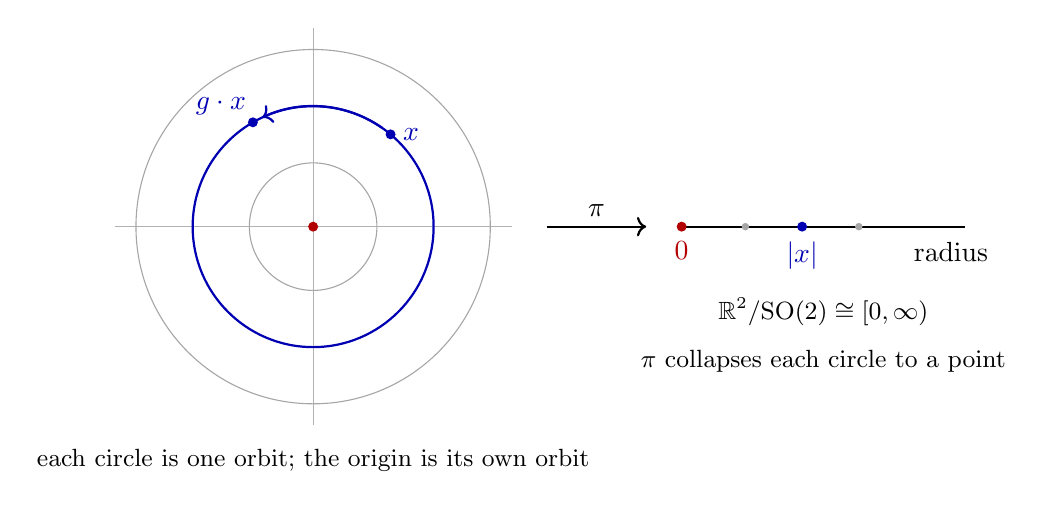
\begin{tikzpicture}[scale=0.9]
    % left panel: the plane with orbits
    \draw[gray!60] (-2.8,0) -- (2.8,0);
    \draw[gray!60] (0,-2.8) -- (0,2.8);
    \draw[gray!70] (0,0) circle (0.9);
    \draw[thick, blue!70!black] (0,0) circle (1.7);
    \draw[gray!70] (0,0) circle (2.5);
    \fill[red!70!black] (0,0) circle (2pt);
    \fill[blue!70!black] (50:1.7) circle (2pt) node[right=1pt] {$x$};
    \fill[blue!70!black] (120:1.7) circle (2pt) node[above left=-1pt] {$g \cdot x$};
    \draw[->, thick, blue!70!black] (55:1.7) arc (55:115:1.7);
    \node at (0,-3.3) {\small each circle is one orbit; the origin is its own orbit};
    % quotient arrow
    \draw[->, thick] (3.3,0) -- (4.7,0) node[midway, above] {$\pi$};
    % right panel: orbit space
    \draw[thick] (5.2,0) -- (9.2,0);
    \fill[red!70!black] (5.2,0) circle (2pt) node[below=2pt] {$0$};
    \fill[gray!70] (6.1,0) circle (1.5pt);
    \fill[blue!70!black] (6.9,0) circle (2pt) node[below=2pt] {$|x|$};
    \fill[gray!70] (7.7,0) circle (1.5pt);
    \node[below=2pt] at (9.0,0) {radius};
    \node at (7.2,-1.2) {\small $\mathbb{R}^2/\SO(2) \cong [0,\infty)$};
    \node at (7.2,-1.9) {\small $\pi$ collapses each circle to a point};
\end{tikzpicture}
\end{center}

\begin{exbox}[$\SO(3)$ Acting on $\mathbb{R}^3$]\exlabel{ex:so3-orbits}
This is the previous example one dimension up, with spheres in place of circles. Let $\SO(3,\mathbb{R})$ act on $\mathbb{R}^3$ by matrix multiplication. Orthogonal matrices preserve the norm ($|gx|^2 = (gx)\cdot(gx) = x \cdot x = |x|^2$), so each orbit lies in a sphere $S_r = \{|x| = r\}$ centered at the origin. In fact:
\begin{itemize}
    \item $\mathcal{O}_0 = \{0\}$.
    \item For $x \neq 0$, $\mathcal{O}_x = S_{|x|}$, the whole sphere of radius $|x|$: given $y$ with $|y| = |x| = r$, let $u = x/r$, $v = y/r$, extend $u$ to an orthonormal basis $(u, u_2, u_3)$ and $v$ to an orthonormal basis $(v, v_2, v_3)$ of $\mathbb{R}^3$ (Gram--Schmidt), replacing $u_3$ by $-u_3$ if necessary so that both bases are positively oriented; then the matrix $g$ with $g u = v$, $g u_2 = v_2$, $g u_3 = v_3$ maps an orthonormal basis to an orthonormal basis, so $g \in \Ogp(3)$, and it maps a positive basis to a positive basis, so $\det g > 0$, i.e.\ $g \in \SO(3)$; and $g x = r\, g u = r v = y$.
\end{itemize}
So the orbits are the concentric spheres together with the origin, and the orbit space is parametrized by the radius:
\[
\mathbb{R}^3/\SO(3) \;\cong\; [0, \infty).
\]
\end{exbox}

\begin{proof}[Proof that $\mathbb{R}^3/\SO(3) \cong [0,\infty)$]
\textit{(Not from lecture; filled in.)} Define $\rho : \mathbb{R}^3/\SO(3) \to [0,\infty)$ by $\rho([x]) = |x|$. It is well defined because $|gx| = |x|$, and it is a bijection by the description of the orbits ($\rho$ is injective since $[x] = [y]$ iff $|x| = |y|$, and surjective since $\rho([(r,0,0)]) = r$). It is continuous by Proposition~\ref{prop:univ-quotient}, since $\rho \circ \pi = |\cdot| : \mathbb{R}^3 \to [0,\infty)$ is continuous. Its inverse $[0,\infty) \to \mathbb{R}^3/\SO(3)$, $r \mapsto [(r,0,0)]$, is the composite of the continuous map $r \mapsto (r,0,0)$ with the continuous map $\pi$. Hence $\rho$ is a homeomorphism.
\end{proof}

\begin{rembox}\label{rem:actions-2}
This example was Uribe's last-minute illustration, given verbally; the proof above supplies the details. Compare it with $\mathbb{CP}^n$: there $S^1$ acts on $S^{2n+1}$ by $z \mapsto \xi z$, the orbit of $z$ is the circle $\{\xi z \mid |\xi| = 1\}$ traced inside the big sphere, and \emph{every} orbit is a circle of the same kind---no special points. That uniformity is part of why $\mathbb{CP}^n$ comes out a manifold. The rotation examples already show one thing the coming theory must accommodate: orbits can have different ``sizes'' (a point and $2$-spheres), and the orbit space can have boundary ($[0,\infty)$ is a manifold \emph{with boundary}, not a manifold). Conditions ruling this out---free actions, properness---are where the theory of quotient manifolds (Lee Ch.\ 21) is headed.
\end{rembox}

The classical groups through the course: defined in Section~\ref{sec:topgroups}, with the examples of Section~\ref{sec:ex-classical}; topological manifolds as level sets in Theorem~\ref{thm:classical-manifolds}; $\SO(2)$ and $\SO(3)$ acting on $\mathbb{R}^2$ and $\mathbb{R}^3$ in Examples~\ref{ex:so2-orbits} and~\ref{ex:so3-orbits}, and $\SO(3)$ on $S^2$ in Examples~\ref{ex:so3-isotropy} and~\ref{ex:s2-homogeneous}; $\Ogp(n)$ acting on the Grassmannians in Corollary~\ref{cor:grassmannian}; smooth manifolds in Examples~\ref{ex:On-smooth} and~\ref{ex:Un-smooth}; their tangent spaces at the identity in Theorem~\ref{thm:classical-summary}, with the infinitesimal rotations of Example~\ref{ex:so3-infinitesimal}; and the double cover $\mathrm{SU}(2) \to \SO(3)$ in Theorem~\ref{thm:double-cover}.


% ---- Lecture 4 (Wed Sep 9, 2026) begins here ----
\subsection{Orbit Relations Are Open}

Throughout, $G$ is a topological group acting continuously on a topological space $X$ (Definition~\ref{def:action} and the definition following it), and $\sim$ is the orbit relation: $x \sim y \iff \exists\, g \in G$ with $y = g \cdot x$ (Proposition~\ref{prop:orbits-partition}).

\begin{lembox}[Left Translations Are Homeomorphisms]\thmlabel{lem:Lg}
For $g \in G$ define $L_g : X \to X$, $L_g(x) = g \cdot x$. Then:
\begin{enumerate}
    \item $L_g$ is continuous;
    \item $L_g \circ L_{g'} = L_{gg'}$ for all $g, g' \in G$, and $L_e = \mathrm{id}_X$;
    \item $L_g$ is a homeomorphism with inverse $L_{g^{-1}}$.
\end{enumerate}
\leeref{proof of Lemma 21.1}
\end{lembox}

\begin{proof}
\textit{(Lecture~4, in full: Uribe gave this proof ``because I want to model what is expected of you when you write your homework.'')} (1) $L_g$ is the composite
\[
X \longrightarrow G \times X \longrightarrow X, \qquad x \longmapsto (g, x) \longmapsto g \cdot x .
\]
The first map is continuous by Theorem~\ref{thm:univ-product}: its components are the constant map $x \mapsto g$ and the identity. The second is the action, continuous by hypothesis. A composite of continuous maps is continuous.

(2) For $x \in X$, $(L_g \circ L_{g'})(x) = g \cdot (g' \cdot x) = (gg') \cdot x = L_{gg'}(x)$ by the second action axiom, and $L_e(x) = e \cdot x = x$ by the first.

(3) By (2), $L_g \circ L_{g^{-1}} = L_{gg^{-1}} = L_e = \mathrm{id}_X$ and $L_{g^{-1}} \circ L_g = L_{g^{-1}g} = L_e = \mathrm{id}_X$. So $L_g$ is a bijection with inverse $L_{g^{-1}}$, which is continuous by (1) applied to $g^{-1}$.
\end{proof}

\begin{rembox}[A Model Proof]\label{rem:model-proof}
Uribe: ``the reason I want to do this with simple proofs is because I want to model what is expected of you when you write your homework.'' The features to imitate: name the map you are studying ($L_g$); prove continuity by exhibiting it as a composite of maps already known to be continuous; get the inverse from the algebra (the action axioms), not from a separate argument; and say which axiom is used where.
\end{rembox}

\begin{lembox}[Orbit Relations Are Open]\thmlabel{lem:orbit-open}
For a continuous action of $G$ on $X$, the orbit relation is an open equivalence relation (Definition of open relation in \S\ref{sub:open-relations}). Equivalently: for every open $U \subseteq X$, its saturation $\tilde U = \pi^{-1}(\pi(U))$ is open.
\leeref{Lemma 21.1, the same statement and proof}
\end{lembox}

\begin{proof}
\textit{(Lecture~4: the saturation of $U$ is the union of the open sets $L_g(U)$.)} By Proposition~\ref{prop:saturation} it suffices to show the saturation of every open $U$ is open. \textbf{Claim:} $\tilde U = \bigcup_{g \in G} L_g(U)$. By definition of saturation and of the orbit relation,
\[
\tilde U = \{\, y \in X \mid \exists\, x \in U \text{ with } y \sim x \,\} = \{\, y \in X \mid \exists\, x \in U,\ g \in G \text{ with } y = g \cdot x \,\},
\]
using symmetry of $\sim$ to write $y \sim x$ as $y = g \cdot x$. And $y = g \cdot x$ for some $x \in U$ means exactly $y \in L_g(U)$; so $\tilde U = \bigcup_g L_g(U)$, proving the claim. Each $L_g(U)$ is open, since $L_g$ is a homeomorphism (Lemma~\ref{lem:Lg}) and homeomorphisms are open maps (Proposition~\ref{fact:cont}(2)). A union of open sets is open.
\end{proof}

\subsection{Hausdorff Orbit Spaces}

\begin{corbox}[Compact Group and Compact Hausdorff Space]\thmlabel{cor:orbit-T2}
If $G$ acts continuously on $X$, and $G$ and $X$ are compact and $X$ is Hausdorff, then the orbit space $X/G$ is Hausdorff.
\leeref{Proposition 21.4 with Corollary 21.6, for Lie groups acting on manifolds}
\end{corbox}

\begin{proof}
We apply the Hausdorff Criterion (Theorem~\ref{thm:hausdorff-criterion}) to the orbit relation $\sim$ on $X$. It has two hypotheses, and its conclusion is exactly that $X/{\sim} = X/G$ is $T_2$.

\emph{Hypothesis 1: $\sim$ is an open relation.} This is Lemma~\ref{lem:orbit-open}, which uses only continuity of the action.

\emph{Hypothesis 2: the graph of $\sim$ is closed in $X \times X$.} The graph is
\[
\Gamma = \{\, (x, y) \in X \times X \mid x \sim y \,\} = \{\, (x, g \cdot x) \mid x \in X,\ g \in G \,\}.
\]
Consider
\[
\Psi : G \times X \longrightarrow X \times X, \qquad \Psi(g, x) = (x, g \cdot x). \tag{$\ast$}
\]
$\Psi$ is continuous by Theorem~\ref{thm:univ-product}, its components being the projection to $X$ and the action. Its image is $\Gamma$: a pair lies in the image iff it has the form $(x, g \cdot x)$ iff it lies in $\Gamma$. Since $G \times X$ is compact (Proposition~\ref{fact:compact}(3)), $\Gamma = \Psi(G \times X)$ is compact (Proposition~\ref{fact:compact}(2)). Since $X$ is Hausdorff, so is $X \times X$ (Theorem~\ref{thm:product-inherit}), and a compact subset of a Hausdorff space is closed (Proposition~\ref{fact:compact}(4)). So $\Gamma$ is closed.

Both hypotheses of Theorem~\ref{thm:hausdorff-criterion} hold, so $X/G$ is Hausdorff.
\end{proof}

\begin{exbox}[Compactness Is Needed: a Non-Hausdorff Orbit Space]\exlabel{ex:nonhausdorff-orbit}
Let the multiplicative group $\mathbb{R}^{+}$ of positive reals act on $X = \mathbb{R}^2 \setminus \{0\}$ by
\[
t \cdot (x, y) = (tx,\, y/t).
\]
This is a continuous action ($X$ is preserved because $t > 0$, and the axioms are immediate), $X$ is Hausdorff and second countable, and the orbit relation is open by Lemma~\ref{lem:orbit-open}. Nonetheless $X/\mathbb{R}^{+}$ is \emph{not} Hausdorff.
\leeref{cf.\ Example 21.3}
\end{exbox}
\begin{center}
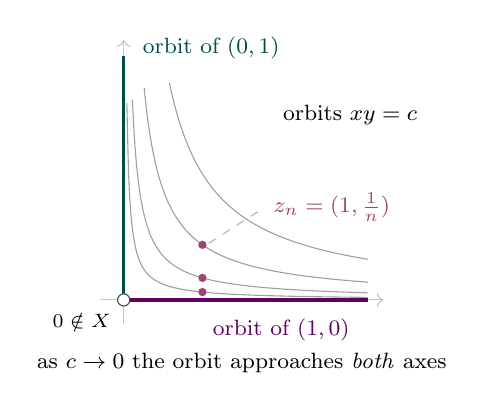
\begin{tikzpicture}[scale=1.0]
\draw[gray!45,->] (-0.3,0) -- (3.3,0); \draw[gray!45,->] (0,-0.3) -- (0,3.3);
\foreach \c/\d in {1.6/0.58, 0.7/0.26, 0.28/0.11, 0.1/0.04} {
  \draw[gray!75,domain=\d:3.1,samples=140,smooth,variable=\x] plot (\x,{\c/\x}); }
\draw[violet!75!black,very thick] (0.04,0) -- (3.1,0);
\draw[teal!60!black,very thick] (0,0.04) -- (0,3.1);
\draw[black!70, fill=white] (0,0) circle (2.2pt); \node[font=\scriptsize, anchor=north east] at (-0.04,-0.04) {$0 \notin X$};
\foreach \y in {0.7,0.28,0.1} { \fill[magenta!60!black] (1,\y) circle (1.5pt); }
\draw[gray!60,dashed] (1.08,0.72) -- (1.75,1.15);
\node[magenta!60!black,font=\footnotesize,anchor=west] at (1.78,1.18) {$z_n=(1,\tfrac1n)$};
\node[violet!75!black,font=\footnotesize,anchor=north] at (2.0,-0.12) {orbit of $(1,0)$};
\node[teal!60!black,font=\footnotesize,anchor=west] at (0.12,3.2) {orbit of $(0,1)$};
\node[font=\footnotesize,anchor=north west] at (1.9,2.6) {orbits $xy=c$};
\node[font=\footnotesize] at (1.5,-0.8) {as $c\to0$ the orbit approaches \emph{both} axes};
\end{tikzpicture}
\end{center}


\begin{proof}[Proof (PSet 1, Problem 3)]
The orbits of $(1,0)$ and $(0,1)$ are the positive $x$-axis $\{(t,0) \mid t>0\}$ and the positive $y$-axis $\{(0,s) \mid s>0\}$; they are distinct classes, since $t \cdot (1,0) = (t,0)$ never has a nonzero second coordinate. Consider $z_n = (1, \tfrac1n) \in X$.

\emph{$[z_n] \to [(1,0)]$.} Let $W \ni [(1,0)]$ be open. Then $\pi^{-1}(W)$ is open in $X$ and contains $(1,0)$, so it contains a box around $(1,0)$, which contains $z_n$ for all large $n$; hence $[z_n] \in \pi(\pi^{-1}(W)) = W$ eventually.

\emph{$[z_n] \to [(0,1)]$.} Acting by $t = \tfrac1n$ gives $\tfrac1n \cdot (1, \tfrac1n) = (\tfrac1n, 1)$, so $[z_n] = [(\tfrac1n, 1)]$, and the same argument applied to the representatives $(\tfrac1n, 1) \to (0,1)$ shows $[z_n]$ is eventually in every open set containing $[(0,1)]$.

A sequence in a Hausdorff space has at most one limit (if $p \neq q$ had disjoint neighborhoods, the sequence could not be eventually in both), so $X/\mathbb{R}^{+}$ is not Hausdorff.
\end{proof}

\begin{rembox}[What the Example Shows]\label{rem:what-example-shows}
Every hypothesis of Corollary~\ref{cor:orbit-T2} except compactness of $G$ holds here, so compactness is not removable. Seen through the criterion: the relation is open, so by Theorem~\ref{thm:hausdorff-criterion} the graph $\Gamma$ must fail to be closed --- and indeed $\big((1,\tfrac1n),(\tfrac1n,1)\big) \in \Gamma$ converges to $\big((1,0),(0,1)\big) \notin \Gamma$. The mechanism is that the orbits, the hyperbolas $xy = c$ together with the two half-axes, \emph{accumulate on each other}: the hyperbola through $z_n$ approaches both axes at once. Compactness of $G$ is what prevents an orbit from running off to infinity and limiting onto a different orbit; properness is the general condition that does the same job for non-compact $G$.

Note also that openness of the relation is \emph{automatic} here (Lemma~\ref{lem:orbit-open}) and buys nothing by itself: the two hypotheses of Theorem~\ref{thm:hausdorff-criterion} are genuinely independent, and for orbit spaces it is always the closed-graph half that carries the content.
\end{rembox}

\begin{thmbox}[Compactness of $X$ Is Not Needed]\thmlabel{thm:orbit-T2-strong}
If a compact topological group $G$ acts continuously on a Hausdorff space $X$, then the orbit space $X/G$ is Hausdorff.
\leeref{Proposition 21.4 with Corollary 21.6, for Lie groups acting on manifolds}
\end{thmbox}

\textbf{Not proved in this course.} Stated in lecture as a strengthening of Corollary~\ref{cor:orbit-T2}, with the proof declined: ``another ten minutes of point-set topology which we will not take.'' The gap is exactly the step where compactness of $X$ was used --- in Corollary~\ref{cor:orbit-T2} it made $\Psi(G \times X) = \Gamma$ compact, hence closed; without it one shows directly that $\Gamma$ is closed, using compactness of $G$ alone (a tube-lemma argument). Corollary~\ref{cor:orbit-T2} is the version proved in lecture, and it suffices for every application below, since all the groups met are compact and all the spaces are compact Hausdorff. For completeness, the tube-lemma argument is short enough to give here.

\begin{proof}[Proof of Theorem~\ref{thm:orbit-T2-strong} (filled in; not from lecture)]
\textit{(Stated in Lecture~4 --- ``compactness of $X$ is not strictly necessary''; filled in.)} By Lemma~\ref{lem:orbit-open} the orbit relation is open, so by Theorem~\ref{thm:hausdorff-criterion} it suffices to show that $\Gamma = \{(x, g\cdot x)\}$ is closed in $X \times X$. Let $(x, y) \notin \Gamma$, so that $g \cdot x \ne y$ for every $g \in G$. For each $g$, choose disjoint open sets $U_g \ni g \cdot x$ and $V_g \ni y$, using that $X$ is Hausdorff. By continuity of the action at $(g, x)$, choose open $A_g \ni g$ and $B_g \ni x$ with $a \cdot x' \in U_g$ for all $a \in A_g$ and $x' \in B_g$. The sets $A_g$ cover the compact $G$, so finitely many, $A_{g_1}, \ldots, A_{g_m}$, suffice; put $B = \bigcap_i B_{g_i}$ and $V = \bigcap_i V_{g_i}$, open neighbourhoods of $x$ and $y$. If some $(x', y') \in B \times V$ had $y' = a \cdot x'$, then $a \in A_{g_i}$ for some $i$, whence $y' \in U_{g_i}$; but also $y' \in V \subseteq V_{g_i}$, which is disjoint from $U_{g_i}$. So $B \times V$ misses $\Gamma$, and $\Gamma$ is closed.
\end{proof}

\begin{defbox}[Proper Map and Proper Action]\deflabel{def:proper}
A continuous map is \textbf{proper} if the preimage of every compact set is compact. A continuous action of a topological group $G$ on a space $X$ is \textbf{proper} if the map $\Psi : G \times X \to X \times X$, $\Psi(g,x) = (x, g\cdot x)$, of $(\ast)$ in the proof of Corollary~\ref{cor:orbit-T2} is proper.
\leeref{Ch.~21, \emph{Proper Actions}}
\end{defbox}

\begin{rembox}[Proper Actions]\label{rem:proper-actions}
Uribe: ``this is one of many theorems people are interested in on when quotient spaces are Hausdorff, and this is the simplest one.'' Properness is the notion that replaces compactness of $G$ altogether: every action of a compact group on a Hausdorff space is proper, and proper actions of non-compact groups are what Lee Ch.\ 21 treats. He warned that his own examples will be mostly compact --- ``I tend to be a compact-manifold person.''
\end{rembox}

\begin{rembox}\label{rem:actions-3}
Proposition~\ref{prop:cpn} is a special case: $\Ugp(1) = S^1$ is compact, $S^{2n+1}$ is compact Hausdorff, and the proof given there is exactly the proof of the corollary specialized to that action.
\end{rembox}

% ============================================================================
% Lecture 4 (Wed Sep 9, 2026), second part
% SECTION 7: HOMOGENEOUS SPACES
% ============================================================================
\section{Homogeneous Spaces}\label{sec:homogeneous}

\roadmark{Thread: quotients}{A transitive action identifies a space with a coset space $G/H$, here as a set; its topology and the Grassmannians follow in \ref{sec:GH-topology}.}

\textit{Reference: Lee Ch.\ 21, the section on homogeneous spaces; Lee Example 1.36 (Grassmannians). Logistics: a substitute lectures on Friday Sep 11; smooth structures are scheduled to begin then.}

\begin{rembox}[Why This Section]\label{rem:why-this-section-5}
\emph{Homogeneous spaces} are spaces on which a group acts transitively. They are identified with coset spaces $G/H$, which are themselves orbit spaces (of $H$ acting on $G$), so everything in \ref{sec:actions} applies. This is how spheres, projective spaces, and Grassmannians acquire their topology in one stroke: ``that's a natural way to give a topology to homogeneous spaces.''
\end{rembox}

\subsection{Transitive Actions and Isotropy}

\begin{defbox}[Transitive Action and Homogeneous Space]\deflabel{def:homogeneous}
An action of $G$ on $X$ is \textbf{transitive} if there is only one orbit; equivalently,
\[
\forall\, x, y \in X\ \ \exists\, g \in G \text{ such that } y = g \cdot x .
\]
A topological space $X$ is \textbf{homogeneous} for the topological group $G$ if $G$ acts continuously and transitively on $X$.
\leeref{Ch.~7 and Example 21.15}
\end{defbox}

\begin{rembox}\label{rem:homogeneous}
For a transitive action the orbit space $X/G$ is a single point, ``which is not that interesting.'' The interesting quotient is a different one: $X$ itself will be exhibited as a quotient $G/H$ of the \emph{group}, by the action of a subgroup $H$ on $G$.
\end{rembox}

\begin{defbox}[Isotropy Subgroup]\deflabel{def:isotropy}
For any action of $G$ on $X$ and any $x_0 \in X$, the \textbf{isotropy subgroup} (or \textbf{stabilizer}) of $x_0$ is
\[
H_{x_0} = \{\, g \in G \mid g \cdot x_0 = x_0 \,\},
\]
the set of group elements that do not move $x_0$.
\leeref{Ch.~7, p.~162}
\end{defbox}

\begin{propbox}[The Isotropy Is a Subgroup]\thmlabel{prop:isotropy-subgroup}
$H_{x_0}$ is a subgroup of $G$.
\end{propbox}

\begin{proof}
$e \in H_{x_0}$ since $e \cdot x_0 = x_0$. If $g, g' \in H_{x_0}$ then $(gg') \cdot x_0 = g \cdot (g' \cdot x_0) = g \cdot x_0 = x_0$. If $g \in H_{x_0}$ then $g^{-1} \cdot x_0 = g^{-1} \cdot (g \cdot x_0) = (g^{-1}g) \cdot x_0 = x_0$.
\end{proof}

\begin{defbox}[Orbit Map]\deflabel{def:orbit-map}
Let a topological group $G$ act continuously on $X$, and let $x_0 \in X$. The \textbf{orbit map} of $x_0$ is
\[
\theta_{x_0} : G \to X, \qquad \theta_{x_0}(g) = g \cdot x_0 .
\]
It is continuous, being the action composed with $g \mapsto (g, x_0)$, and its image is the orbit of $x_0$.
\leeref{Proposition 7.26}
\end{defbox}

\begin{thmbox}[Isotropy Subgroups Are Closed]\thmlabel{thm:isotropy-closed}
Let $G$ be a topological group acting continuously on a topological space $X$ in which points are closed (for instance, $X$ Hausdorff). Then for every $x_0 \in X$ the isotropy subgroup $H_{x_0}$ is a \emph{closed} subgroup of $G$.
\leeref{proof of Theorem 21.18 (``closed by continuity)}
\end{thmbox}

\begin{proof}[Exercise]
\textit{(Claimed in Lecture~4 --- ``this is a closed subgroup''; filled in.)} Consider the orbit map $\theta_{x_0} : G \to X$, $\theta_{x_0}(g) = g \cdot x_0$, of Definition~\ref{def:orbit-map}, and identify $H_{x_0}$ as a preimage under it. Two things are to be checked: that $\theta_{x_0}$ is continuous, and that the relevant subset of $X$ is closed. Uribe stated the result and said the closedness ``may be the next assignment''; it was not proved in lecture, and the argument is left here.
\end{proof}

\textbf{On the hypothesis.} The board stated the theorem with no condition on $X$, and in that form it is false, as the next example shows. What fails there is precisely that points of $X$ are not closed. Requiring $X$ to be $T_1$ --- in particular Hausdorff, which is the case for every manifold --- repairs the statement, and costs nothing in the applications: $\Ogp(n)$ acting on $\Gr_k(\mathbb{R}^n)$, $\SO(3)$ on $S^2$, and every other action met here has Hausdorff target.

\begin{exbox}[An Isotropy Group That Is Not Closed]\exlabel{ex:isotropy-not-closed}
Let $G = \mathbb{R}$ act on $X = \mathbb{R}/\mathbb{Q}$, with the quotient topology, by $t \cdot [x] = [x+t]$. The action is continuous, but the isotropy group $H_{[0]} = \mathbb{Q}$ is not closed in $\mathbb{R}$. So Theorem~\ref{thm:isotropy-closed} fails without its hypothesis on $X$.
\end{exbox}

\begin{proof}
\textit{(Not from lecture; filled in.)} The action is well defined, since $x - x' \in \mathbb{Q}$ implies $(x+t) - (x'+t) \in \mathbb{Q}$. Every nonempty open saturated subset of $\mathbb{R}$ contains an interval and is invariant under adding rationals; since $\mathbb{Q}$ is dense, the translates of an interval by rationals cover $\mathbb{R}$, so the set is all of $\mathbb{R}$. Hence $X$ carries the indiscrete topology, every map into $X$ is continuous, and in particular so is the action. Finally
\[
H_{[0]} = \{\, t \in \mathbb{R} \mid [t] = [0] \,\} = \mathbb{Q},
\]
which is dense in $\mathbb{R}$ and not closed.
\end{proof}

The classical groups through the course: defined in Section~\ref{sec:topgroups}, with the examples of Section~\ref{sec:ex-classical}; topological manifolds as level sets in Theorem~\ref{thm:classical-manifolds}; $\SO(2)$ and $\SO(3)$ acting on $\mathbb{R}^2$ and $\mathbb{R}^3$ in Examples~\ref{ex:so2-orbits} and~\ref{ex:so3-orbits}, and $\SO(3)$ on $S^2$ in Examples~\ref{ex:so3-isotropy} and~\ref{ex:s2-homogeneous}; $\Ogp(n)$ acting on the Grassmannians in Corollary~\ref{cor:grassmannian}; smooth manifolds in Examples~\ref{ex:On-smooth} and~\ref{ex:Un-smooth}; their tangent spaces at the identity in Theorem~\ref{thm:classical-summary}, with the infinitesimal rotations of Example~\ref{ex:so3-infinitesimal}; and the double cover $\mathrm{SU}(2) \to \SO(3)$ in Theorem~\ref{thm:double-cover}.


\begin{exbox}[Isotropy of the North Pole under $\SO(3)$]\exlabel{ex:so3-isotropy}
Let $\SO(3)$ act on $S^2 = \{x \in \mathbb{R}^3 \mid |x| = 1\}$ by rotations (matrix multiplication; it preserves the sphere since orthogonal matrices preserve norms). For $x_0 = (0,0,1)$, the answer from the floor: the isotropy consists of the rotations about the $z$-axis. In matrices, $g \cdot e_3 = e_3$ says the third column of $g$ is $e_3$; orthogonality then forces the third row to be $e_3^T$ as well (the columns are orthonormal, so the first two columns are orthogonal to $e_3$, i.e.\ have zero third entry), and the remaining $2 \times 2$ block is orthogonal with determinant $1$:
\[
H_{x_0} = \left\{ \begin{pmatrix} A & 0 \\ 0 & 1 \end{pmatrix} \;\middle|\; A \in \SO(2) \right\} \;\cong\; \SO(2) \;\cong\; S^1 .
\]
\end{exbox}

\subsection{The Coset Space $G/H$}

\begin{rembox}[The Organizing Fact]\label{rem:organizing-fact}
Everything in this section and the next is a special case of \ref{sec:actions}. The coset space $G/H$ is not merely \emph{like} an orbit space: it \emph{is} one, for a suitable action of $H$ on $G$ (Proposition~\ref{prop:GH-orbit-space}), with the same underlying set and the same projection map --- so the quotient topology of \S\ref{sub:GH-topology} and the orbit-space topology of Definition~\ref{def:orbit-space} are equal by construction, not merely homeomorphic. Consequently every result of \ref{sec:actions} applies to $G/H$ with no further work, and three facts below are obtained that way: $\pi$ is an open map (Lemma~\ref{lem:orbit-open}), $G/H$ is Hausdorff under a compactness hypothesis (Corollary~\ref{cor:orbit-T2}), and it is second countable (Theorem~\ref{thm:2c-quotient}).
\end{rembox}

\begin{defbox}[Left Cosets and the Coset Space]\deflabel{def:cosets}
Let $H \le G$ be a subgroup of a group $G$. The \textbf{left coset} of $g \in G$ is
\[
gH \;=\; \{\, gh \mid h \in H \,\} \;\subseteq\; G,
\]
the translate of $H$ by $g$. The \textbf{coset space} $G/H$ is the set whose elements are the left cosets,
\[
G/H \;=\; \{\, gH \mid g \in G \,\}.
\]
(This is the algebraic quotient from MATH 493. Note that $G/H$ is a \emph{group} only when $H$ is normal, which is not assumed here; for us it is only a set, and shortly a space.)
\leeref{proof of Theorem 21.17}
\end{defbox}

\begin{lembox}[When Two Cosets Coincide]\thmlabel{lem:cosets}
$gH = g'H \iff g^{-1}g' \in H$. Consequently the left cosets partition $G$.
\leeref{proof of Theorem 21.17}
\end{lembox}

\begin{proof}
\textit{(Used in Lecture~4 as ``$gH = g'H \iff g^{-1}g' \in H$''; filled in.)} ($\Rightarrow$) $g' = g'e \in g'H = gH$, so $g' = gh$ for some $h \in H$, i.e.\ $g^{-1}g' = h \in H$. ($\Leftarrow$) If $g^{-1}g' = h \in H$, then $g' = gh$, so $g'H = ghH = gH$ (as $hH = H$ for $h \in H$, $H$ being a subgroup). For the partition: $g \in gH$, and if $gH \cap g'H \ni a$, then $aH = gH$ and $aH = g'H$ by the first part, so $gH = g'H$.
\end{proof}

\begin{defbox}[The Canonical Projection]\deflabel{def:coset-projection}
The \textbf{canonical projection} associated with $H \le G$ is the map
\[
\pi : G \longrightarrow G/H, \qquad \pi(g) = gH,
\]
sending a group element to the coset containing it. It is surjective by construction, and by Lemma~\ref{lem:cosets} its fibres are exactly the cosets: $\pi^{-1}(gH) = gH$.
\leeref{Theorem 21.17}
\end{defbox}

\begin{rembox}\label{rem:homogeneous-2}
A point of $G/H$ is a \emph{subset} of $G$, and $\pi$ is the map that forgets which element of that subset one started from. The two roles of the symbol $gH$ --- a subset of $G$, and a single point of $G/H$ --- are the usual source of confusion with quotients (\S\ref{sub:quotients}); the identity $\pi^{-1}(gH) = gH$ is that ambiguity made harmless, the left side reading $gH$ as a point and the right side as a set.
\end{rembox}

\begin{propbox}[$G/H$ Is an Orbit Space]\thmlabel{prop:GH-orbit-space}
Let $H \le G$. The formula
\[
H \times G \longrightarrow G, \qquad (h, g) \longmapsto g h^{-1}
\]
is an action of $H$ on $G$, and its orbits are exactly the left cosets: $\mathcal{O}_g = gH$. Hence $G/H$ (the set of left cosets) is the orbit space of this action.
\leeref{proof of Theorem 21.17 ($H$ acting on $G$ by right translation)}
\end{propbox}

\begin{proof}
\textit{(Lecture~4 checked the action axiom, $(hh')\cdot g = h \cdot (h' \cdot g)$, on the board; the rest is filled in.)} \emph{Action.} $e \cdot g = g e^{-1} = g$. For $h, h' \in H$: $(hh') \cdot g = g (hh')^{-1} = g\, h'^{-1} h^{-1} = (g h'^{-1}) h^{-1} = h \cdot (h' \cdot g)$. (The inverse is what makes the order of the factors come out right: multiplying on the right by $h$ itself would give $g h' h$, which is $(h'h) \cdot g$, the wrong order.) \emph{Orbits.} $\mathcal{O}_g = \{\, g h^{-1} \mid h \in H \,\} = \{\, g h \mid h \in H \,\} = gH$, since $h \mapsto h^{-1}$ is a bijection of $H$.
\end{proof}

\begin{rembox}\label{rem:homogeneous-3}
The inverse in the formula is not cosmetic. The first thing one writes, $(h,g) \mapsto hg$, is also an action, but its orbits are the \emph{right} cosets $Hg$, giving the other quotient $H \backslash G$. To produce \emph{left} cosets from a \emph{left} action of $H$ one must multiply on the right and invert, and that is exactly what makes the second axiom come out in the correct order, as the proof shows. For non-abelian $H$ the naive formula $(h,g) \mapsto gh$ fails the axiom outright.

Proposition~\ref{prop:GH-orbit-space} is a statement about sets; the topological half is Definition~\ref{def:GH-topology} together with the observation that the two projections $G \to G/H$ --- the canonical one of Definition~\ref{def:coset-projection} and the orbit projection of Definition~\ref{def:orbit-space} --- are the same function, so the two quotient topologies they induce are the same topology.
\end{rembox}

\begin{lembox}[Homogeneous Spaces Are Coset Spaces]\thmlabel{lem:GH-bijection}
Suppose $G$ acts transitively on $X$, fix a \emph{base point} $x_0 \in X$, and let $H = H_{x_0}$. Then
\[
\Phi : G/H \longrightarrow X, \qquad \Phi(gH) = g \cdot x_0
\]
is a well-defined bijection.
\leeref{proof of Theorem 21.18}
\end{lembox}

\begin{proof}
\textit{(Lecture~4 checked well-definedness --- translate ``the so-called base point'' --- on the board; injectivity and surjectivity are filled in.)} \emph{Well defined.} If $gH = g'H$ then $g' = gh$ with $h \in H$ (Lemma~\ref{lem:cosets}), and
\[
g' \cdot x_0 = (gh) \cdot x_0 = g \cdot (h \cdot x_0) = g \cdot x_0,
\]
since $h$ fixes $x_0$. \emph{Injective.} If $g \cdot x_0 = g' \cdot x_0$, apply $L_{g^{-1}}$: $x_0 = g^{-1} \cdot (g' \cdot x_0) = (g^{-1}g') \cdot x_0$, so $g^{-1}g' \in H$ and $gH = g'H$ by Lemma~\ref{lem:cosets}. \emph{Surjective.} Given $y \in X$, transitivity gives $g$ with $y = g \cdot x_0 = \Phi(gH)$.
\end{proof}

\begin{exbox}[The Sphere as a Homogeneous Space]\exlabel{ex:s2-homogeneous}
$\SO(3)$ acts transitively on $S^2$: the orbit of $e_3$ is the whole sphere (the argument of Example~\ref{ex:so3-orbits} with $r = 1$). By Example~\ref{ex:so3-isotropy} the isotropy of $e_3$ is the copy $H$ of $\SO(2)$ in the upper-left block. Hence, as sets (and, by the theorem below, as spaces),
\[
S^2 \;\cong\; \SO(3)/\SO(2).
\]
\emph{Explicitly.} A point of $\SO(3)/H$ is a coset $gH = \{\, gh \mid h \in H \,\}$. Since $h e_3 = e_3$ for $h \in H$, every element of $gH$ has the same third column $g e_3$; conversely, if $g' e_3 = g e_3$ then $g^{-1} g' \in H$, so $g' \in gH$ (Lemma~\ref{lem:cosets}). Thus
\[
gH = \{\, \text{rotations whose third column is } g e_3 \,\},
\]
and the cosets are indexed by unit vectors. The identification $\Phi(gH) = g \cdot e_3 = g e_3$ reads off that third column; its inverse sends a unit vector $v \in S^2$ to the set of all rotations having $v$ as third column (nonempty, since some rotation carries $e_3$ to $v$). A set of unit vectors $W \subseteq S^2$ is open in the quotient topology iff the set of all rotations whose third column lies in $W$ is open in $\SO(3)$; Theorem~\ref{thm:GH-homeo} says this agrees with the usual topology of $S^2 \subseteq \mathbb{R}^3$.
\leeref{Examples 21.15(a) and 21.19(a)}
\end{exbox}

\textbf{Transcription note.} Page~12 of the handwritten notes writes ``$X = \SO(3)$ acting on $S^2$''; the group is $G = \SO(3)$ and the space is $X = S^2$.

\begin{center}
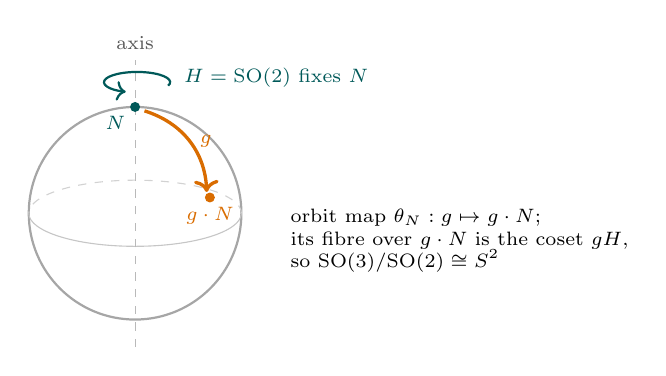
\begin{tikzpicture}
\draw[thick, gray!70] (0,0) circle (1.35); \draw[gray!45] (-1.35,0) arc (180:360:1.35 and 0.42); \draw[gray!35, dashed] (1.35,0) arc (0:180:1.35 and 0.42);
\draw[gray!55, dashed] (0,-1.7) -- (0,1.95) node[above, font=\scriptsize, text=gray!70!black] {axis};
\draw[->, thick, teal!70!black] (0.42,1.62) arc (-20:250:0.42 and 0.13); \node[teal!70!black, font=\scriptsize, anchor=west] at (0.5,1.72) {$H = \SO(2)$ fixes $N$};
\fill[teal!70!black] (0,1.35) circle (1.8pt) node[anchor=north east, font=\scriptsize] {$N$};
\draw[->, very thick, orange!85!black] (0.12,1.3) to[bend left=35] node[right, font=\scriptsize] {$g$} (0.910,0.270);
\fill[orange!85!black] (0.950,0.200) circle (1.8pt) node[anchor=north, font=\scriptsize] {$g \cdot N$};
\node[font=\scriptsize, align=left, anchor=west] at (1.85,-0.35) {orbit map $\theta_N : g \mapsto g\cdot N$;\\ its fibre over $g\cdot N$ is the coset $gH$,\\ so $\SO(3)/\SO(2) \cong S^2$};
\end{tikzpicture}
\end{center}

The picture behind Example~\ref{ex:s2-homogeneous}. The rotations about the vertical axis fix the north pole $N$; they form the isotropy group $H \cong \SO(2)$. A rotation $g$ carries $N$ to $g \cdot N$, and the rotations carrying $N$ to that same point are exactly the products $gh$ with $h \in H$: the fibre of the orbit map $\theta_N$ over $g \cdot N$ is the coset $gH$. Collapsing each fibre to a point is the passage from $\SO(3)$ to $\SO(3)/\SO(2)$, which is why the coset space is the sphere (Theorem~\ref{thm:GH-homeo}).

% ============================================================================
% SECTION: THE TOPOLOGY OF $G/H$ AND REAL GRASSMANNIANS
% ============================================================================

\section{The Topology of $G/H$ and Real Grassmannians}\label{sec:GH-topology}\label{sub:GH-topology}

\roadmark{Thread: quotients}{The coset space $G/H$ as a topological space: open quotient, Hausdorff when $H$ is closed, and homeomorphic to a homogeneous space. The Grassmannians are the payoff. The two threads meet in the next chapter.}

Definitions \ref{def:cosets} and \ref{def:coset-projection} are purely algebraic. If $G$ carries a topology, $G/H$ inherits one in the only reasonable way.

\begin{defbox}[The Quotient Topology on a Coset Space]\deflabel{def:GH-topology}
Let $G$ be a topological group and $H \le G$ a subgroup. The \textbf{quotient topology} on $G/H$ is the quotient topology induced by the canonical projection $\pi$ of Definition~\ref{def:coset-projection}, in the sense of Definition~\ref{def:quotient}:
\[
W \subseteq G/H \text{ is open} \iff \pi^{-1}(W) \subseteq G \text{ is open in } G.
\]
Unless stated otherwise, $G/H$ always carries this topology.
\leeref{Theorem 21.17}
\end{defbox}

\begin{propbox}[Three Descriptions of the Open Sets]\thmlabel{prop:GH-open-sets}
Let $G$ be a topological group, $H \le G$, and $W \subseteq G/H$. The following are equivalent:
\begin{enumerate}
    \item $W$ is open in $G/H$;
    \item $\displaystyle\bigcup_{gH \in W} gH$, the union in $G$ of the cosets belonging to $W$, is open in $G$;
    \item $W = \pi(U)$ for some open $U \subseteq G$ satisfying $UH = U$.
\end{enumerate}
Moreover $\pi$ is a continuous, surjective, \emph{open} map, and the quotient topology is the finest topology on $G/H$ making $\pi$ continuous.
\leeref{Theorem 21.17 and Lemma 21.1}
\end{propbox}

\begin{proof}
\textit{(Not from lecture; filled in.)} $(1 \Leftrightarrow 2)$ By Definition~\ref{def:coset-projection} the fibre over a point $gH \in W$ is the coset $gH$, so $\pi^{-1}(W) = \bigcup_{gH \in W} gH$; now apply Definition~\ref{def:GH-topology}.

$(1 \Leftrightarrow 3)$ A subset $U \subseteq G$ satisfies $UH = U$ iff it is a union of cosets, i.e.\ iff it is saturated for the coset relation (Definition~\ref{def:saturation}): $UH = \bigcup_{u \in U} uH$ always contains $U$, and equals $U$ exactly when each $uH \subseteq U$. If $W$ is open, take $U = \pi^{-1}(W)$, which is open, saturated, and has $\pi(U) = W$ by surjectivity of $\pi$. Conversely if $U$ is open with $UH = U$, then $\pi^{-1}(\pi(U)) = U$ by saturation (Lemma~\ref{lem:saturation}(4)), which is open, so $\pi(U)$ is open.

\emph{Openness of $\pi$.} For $U \subseteq G$ open, $\pi^{-1}(\pi(U)) = UH = \bigcup_{h \in H} Uh$, a union of translates of $U$. Right translation by $h$ is a homeomorphism of $G$ (it is continuous with continuous inverse, both restrictions of the multiplication of the topological group), so each $Uh$ is open and the union is open; hence $\pi(U)$ is open. Continuity and finest-topology are the general facts recorded after Definition~\ref{def:quotient}.
\end{proof}

\begin{corbox}[$\pi$ Is a Quotient Map]\thmlabel{cor:GH-quotient-map}
$\pi : G \to G/H$ is a quotient map in the sense of Definition~\ref{def:quotient-map}, and consequently a map $g : G/H \to Z$ into a topological space is continuous if and only if $g \circ \pi : G \to Z$ is continuous.
\leeref{Theorem 21.17}
\end{corbox}

\begin{proof}
\textit{(Not from lecture; filled in.)} $\pi$ is a continuous open surjection by Proposition~\ref{prop:GH-open-sets}, hence a quotient map by Proposition~\ref{prop:open-surj-quotient}. (It is also one directly from Definition~\ref{def:GH-topology}, which is the defining property.) The second statement is the universal property, Proposition~\ref{prop:univ-quotient}.
\end{proof}

\begin{rembox}\label{rem:homogeneous-4}
\textbf{Openness of $\pi$, for free.} The action of $H$ on $G$ in Proposition~\ref{prop:GH-orbit-space} is continuous, being the restriction to $H \times G$ of the map $(h,g) \mapsto gh^{-1}$ on $G \times G$, a composite of inversion and multiplication. So by the organizing fact, Definition~\ref{def:GH-topology} \emph{is} the orbit-space topology, and Lemma~\ref{lem:orbit-open} --- every orbit relation of a continuous action is open --- already gives that $\pi$ is an open map. The proof above is that argument written out in the group case, with the translations $L_h$ of Lemma~\ref{lem:Lg} appearing as right translations $g \mapsto gh$; it is included because the formula $\pi^{-1}(\pi(U)) = UH$ is worth seeing explicitly.
\end{rembox}

\begin{thmbox}[Homogeneous Spaces Are Homeomorphic to Coset Spaces]\thmlabel{thm:GH-homeo}
Let $G$ act continuously and transitively on a topological space $X$, let $x_0 \in X$, $H = H_{x_0}$, and let $\Phi : G/H \to X$, $\Phi(gH) = g \cdot x_0$.
\begin{enumerate}
    \item $\Phi$ is a continuous bijection.
    \item If $G/H$ is compact and $X$ is Hausdorff, then $\Phi$ is a homeomorphism.
\end{enumerate}
In particular (2) applies whenever $G$ itself is compact.
\leeref{Theorem 21.18, a smooth version without compactness (see the comparison below)}
\end{thmbox}

\begin{center}
\begin{tikzcd}[row sep=2.6em, column sep=2.2em]
& G \arrow[dl, "\pi"'] \arrow[dr, "g \,\mapsto\, g \cdot x_0"] & \\
G/H \arrow[rr, "\Phi"'] & & X
\end{tikzcd}
\end{center}

Upstairs is the group, downstairs its coset space, and the triangle commutes: $\Phi \circ \pi$ is the orbit map. The orbit map is continuous for free; part (1) is the universal property pushing that continuity down along $\pi$, and part (2) is the compactness argument upgrading the bottom arrow to a homeomorphism.


\begin{proof}
\textit{(Stated in Lecture~4, with a hypothesis missing --- the board said ``$G$ compact $\Rightarrow$ $G/H \cong X$'', and $X$ must also be Hausdorff; filled in.)}
(1) Bijectivity is Lemma~\ref{lem:GH-bijection}. The composite $\Phi \circ \pi : G \to X$ is the orbit map $g \mapsto g \cdot x_0$, which is continuous: it is $G \to G \times X \to X$, $g \mapsto (g, x_0) \mapsto g \cdot x_0$, a composite of a map continuous by Theorem~\ref{thm:univ-product} with the action. By the universal property of the quotient (Proposition~\ref{prop:univ-quotient}), $\Phi$ is continuous.

(2) By (1), $\Phi$ is a continuous bijection from the compact space $G/H$ onto the Hausdorff space $X$, hence a homeomorphism (Proposition~\ref{fact:compact}(6)). Spelled out: if $C \subseteq G/H$ is closed, then $C$ is compact by Proposition~\ref{fact:compact}(5), so $\Phi(C)$ is compact by (2) of that proposition, hence closed in $X$ by (4); so $\Phi$ is a closed map, and the inverse of a closed continuous bijection is continuous, since $(\Phi^{-1})^{-1}(C) = \Phi(C)$ for every $C$.

For the final sentence of the theorem: if $G$ is compact, then $G/H = \pi(G)$ is compact as the continuous image of a compact space.
\end{proof}

\begin{exbox}[The Circle as $\mathbb{R}/\mathbb{Z}$]\exlabel{ex:circle-RZ}
Let the additive group $\mathbb{R}$ act on $S^1 = \{z \in \mathbb{C} \mid |z| = 1\}$ by
\[
t \cdot z = e^{2\pi i t} z .
\]
This is an action ($0 \cdot z = z$ and $s \cdot (t \cdot z) = e^{2\pi i s}e^{2\pi i t}z = (s+t) \cdot z$), it is continuous (the map $(t,z) \mapsto e^{2\pi i t}z$ is continuous on $\mathbb{R} \times S^1$), and it is transitive (every $w \in S^1$ is $e^{2\pi i \theta} = \theta \cdot 1$ for some $\theta$). The isotropy of the base point $1$ is
\[
H_1 = \{\, t \in \mathbb{R} \mid e^{2\pi i t} = 1 \,\} = \mathbb{Z} .
\]
The coset space $\mathbb{R}/\mathbb{Z}$ is compact, being the image under $\pi$ of the compact interval $[0,1]$ (every coset $t + \mathbb{Z}$ meets $[0,1]$), and $S^1$ is Hausdorff. So Theorem~\ref{thm:GH-homeo}(2) gives a homeomorphism
\[
\Phi : \mathbb{R}/\mathbb{Z} \xrightarrow{\ \cong\ } S^1, \qquad t + \mathbb{Z} \longmapsto e^{2\pi i t} .
\]
Here $G = \mathbb{R}$ is \emph{not} compact, so the version of the theorem with ``$G$ compact'' would not apply. The hypothesis on the quotient is genuinely weaker than the hypothesis on the group, and it is the one that matters: the proof uses compactness of $G/H$ and nothing about $G$.
\leeref{Example 21.14(a)}
\end{exbox}

\begin{center}
\begin{tikzcd}[row sep=2.6em, column sep=2.2em]
& \mathbb{R} \arrow[dl, "\pi"'] \arrow[dr, "t \,\mapsto\, e^{2\pi i t}"] & \\
\mathbb{R}/\mathbb{Z} \arrow[rr, "\Phi"', "\cong"] & & S^1
\end{tikzcd}
\end{center}

The same triangle with $G = \mathbb{R}$. The exponential wraps the line around the circle; it is constant exactly on the cosets $t + \mathbb{Z}$, which is why it descends to the quotient, and the induced bottom arrow is the homeomorphism.

\begin{exbox}[A Continuous Bijection That Is Not a Homeomorphism]\exlabel{ex:GH-not-homeo}
Let $G = \mathbb{R}_{\mathrm{disc}}$, the additive group of real numbers with the discrete topology --- a topological group, since every map out of a discrete space is continuous. It acts on $X = \mathbb{R}$, with its usual topology, by translation, $t \cdot x = x + t$. The action is continuous, because $G \times X$ is the disjoint union of the open sets $\{t\} \times X$, on each of which it is a translation. It is transitive, the isotropy group of $0$ is $\{0\}$, and so $G/H = \mathbb{R}_{\mathrm{disc}}$. The map $\Phi : \mathbb{R}_{\mathrm{disc}} \to \mathbb{R}$, $t \mapsto t$, is a continuous bijection but not a homeomorphism: $\{0\}$ is open in $\mathbb{R}_{\mathrm{disc}}$ and not in $\mathbb{R}$. Here $X$ is Hausdorff and $G/H$ is not compact, so Theorem~\ref{thm:GH-homeo}(2) does not apply --- and its conclusion genuinely fails.
\leeref{no counterpart; a course example}
\end{exbox}

\textbf{Comparison with Lee.} Lee's Theorem~21.18 has no compactness hypothesis: for a Lie group acting smoothly and transitively on a manifold, $\Phi$ is an equivariant \emph{diffeomorphism}. Smoothness does the work that compactness does here --- $\Phi$ has constant rank by his equivariant rank theorem (Theorem~7.25), and a bijection of constant rank is a diffeomorphism. His standing assumption that $G$ is a Lie group, in particular second countable, also rules out Example~\ref{ex:GH-not-homeo}, where $G$ is an uncountable discrete group. In the purely topological setting of the course some hypothesis is needed, and ``$G/H$ compact, $X$ Hausdorff'' is the one used.


\textbf{Classroom exchange and its resolution.} On the board the statement read ``if $G$ is compact, then $G/H \cong X$ is a homeomorphism,'' with no hypothesis on $X$ beyond the continuous transitive action. A student objected that the conclusion cannot hold with no condition on the topology of $X$; Uribe agreed on the spot (``good catch \ldots\ I think I made a mistake, and I will correct that by email''). The correction arrived as Problem~1 of Assignment~2, which states exactly the theorem above: (1) with no hypotheses, and (2) under ``$G/H$ compact and $X$ Hausdorff.'' So the board version was off in two ways at once --- it was missing Hausdorffness of $X$, and it asked for compactness of the wrong space. Example~\ref{ex:circle-RZ} shows the second repair matters.

\begin{defbox}[The Topology of a Homogeneous Space]\deflabel{def:homogeneous-topology}
Let a topological group $G$ act transitively on a \emph{set} $X$, let $x_0 \in X$, and let $H = H_{x_0}$. The \textbf{homogeneous-space topology} on $X$ is the one that makes the bijection $\Phi : G/H \to X$, $gH \mapsto g \cdot x_0$, of Lemma~\ref{lem:GH-bijection} a homeomorphism: $V \subseteq X$ is open iff $\Phi^{-1}(V)$ is open in $G/H$.
\leeref{Theorem 21.20}
\end{defbox}

\begin{propbox}[Independence of the Base Point]\thmlabel{prop:homog-basepoint}
The homogeneous-space topology does not depend on the choice of $x_0$.
\leeref{Theorem 21.20}
\end{propbox}

\begin{proof}
\textit{(Not from lecture; filled in.)} Let $x_1 = a \cdot x_0$. Then $H_{x_1} = aH_{x_0}a^{-1}$, since $g\,a\cdot x_0 = a\cdot x_0 \iff a^{-1}ga \in H_{x_0}$. Right translation $g \mapsto ga^{-1}$ is a homeomorphism of $G$ carrying each coset $gH_{x_0}$ onto $ga^{-1}(aH_{x_0}a^{-1}) = ga^{-1}H_{x_1}$. So, by the universal property (Corollary~\ref{prop:univ-quotient}), it induces a continuous map $\bar R : G/H_{x_0} \to G/H_{x_1}$, $gH_{x_0} \mapsto ga^{-1}H_{x_1}$, whose inverse is induced in the same way by $g \mapsto ga$. Hence $\bar R$ is a homeomorphism. It intertwines the two bijections, since $\Phi_1(\bar R(gH_{x_0})) = ga^{-1}\cdot x_1 = g \cdot x_0 = \Phi_0(gH_{x_0})$. So $\Phi_1 = \Phi_0 \circ \bar R^{-1}$, and the two transported topologies coincide.
\end{proof}

\begin{rembox}[Giving a Set a Topology]\label{rem:giving-set-topology}
Theorem~\ref{thm:GH-homeo} is also used in reverse: when $X$ is merely a \emph{set} on which $G$ acts transitively, the definition above gives it a topology --- ``that's a natural way to give a topology to homogeneous spaces.'' This is how the Grassmannians below get their topology, and the proposition says the result is canonical.
\end{rembox}

\begin{corbox}[When $G/H$ Is Hausdorff and Second Countable]\thmlabel{cor:GH-nice}
Let $G$ be a compact Hausdorff topological group and $H \le G$ a compact subgroup. Then $G/H$ is compact Hausdorff; if moreover $G$ is second countable, so is $G/H$.
\leeref{Theorem 21.17}
\end{corbox}

\begin{proof}
\textit{(Not from lecture; filled in.)} Everything is an application of \ref{sec:actions} to the continuous action of $H$ on $G$ of Proposition~\ref{prop:GH-orbit-space}, whose orbit space is $G/H$ with its quotient topology. Apply Corollary~\ref{cor:orbit-T2}: $H$ and $G$ compact, $G$ Hausdorff, so the orbit space $G/H$ is Hausdorff; it is compact as $\pi(G)$. Second countability is Theorem~\ref{thm:2c-quotient}, the orbit relation being open by Lemma~\ref{lem:orbit-open}.
\end{proof}

The classical groups through the course: defined in Section~\ref{sec:topgroups}, with the examples of Section~\ref{sec:ex-classical}; topological manifolds as level sets in Theorem~\ref{thm:classical-manifolds}; $\SO(2)$ and $\SO(3)$ acting on $\mathbb{R}^2$ and $\mathbb{R}^3$ in Examples~\ref{ex:so2-orbits} and~\ref{ex:so3-orbits}, and $\SO(3)$ on $S^2$ in Examples~\ref{ex:so3-isotropy} and~\ref{ex:s2-homogeneous}; $\Ogp(n)$ acting on the Grassmannians in Corollary~\ref{cor:grassmannian}; smooth manifolds in Examples~\ref{ex:On-smooth} and~\ref{ex:Un-smooth}; their tangent spaces at the identity in Theorem~\ref{thm:classical-summary}, with the infinitesimal rotations of Example~\ref{ex:so3-infinitesimal}; and the double cover $\mathrm{SU}(2) \to \SO(3)$ in Theorem~\ref{thm:double-cover}.


\subsection{Real Grassmannians}

\begin{defbox}[Grassmannian]\deflabel{def:grassmannian}
For $0 \le k \le n$, the \textbf{real Grassmannian} is the set
\[
\Gr_k(\mathbb{R}^n) = \{\, V \subseteq \mathbb{R}^n \mid V \text{ is a } k\text{-dimensional linear subspace} \,\}.
\]
For $k = 1$ it is the set of lines through the origin in $\mathbb{R}^n$, the \textbf{real projective space}
\[
\Gr_1(\mathbb{R}^n) = \mathbb{RP}^{n-1}.
\]
\leeref{Example 1.36}
\end{defbox}

\begin{rembox}[On the Index]\label{rem:index}
The board first said $\Gr_1(\mathbb{R}^n) = \mathbb{RP}^n$; a student asked whether it should be $n-1$, and after some back-and-forth (``this drives me absolutely crazy'') the answer settled on $\mathbb{RP}^{n-1}$: each line through $0$ in $\mathbb{R}^n$ meets the unit sphere $S^{n-1}$ in exactly two antipodal points $\pm v$, so $\mathbb{RP}^{n-1} \cong S^{n-1}/\{\pm I\}$, an $(n-1)$-dimensional object. Explicitly, the quotient on the right is the orbit space of the group $\{\pm I\} \cong \mathbb{Z}/2$ acting on $S^{n-1}$ by $v \mapsto \pm v$: a point is an antipodal pair $\{v, -v\}$, $\pi(v) = \{v,-v\}$, a set of pairs is open iff the union of the pairs is open in $S^{n-1}$, and the identification with $\Gr_1(\mathbb{R}^n)$ is $\{v, -v\} \mapsto \mathbb{R} v$, with inverse $\ell \mapsto \ell \cap S^{n-1}$. This orbit space is Hausdorff by Corollary~\ref{cor:orbit-T2} ($\{\pm I\}$ finite, hence compact), and its topology agrees with the homogeneous-space topology of $\Gr_1(\mathbb{R}^n)$ (see the note after Corollary~\ref{cor:rpn-atlas}). The superscript on $\mathbb{RP}$ records the dimension of the manifold; the superscript on the $\mathbb{R}^n$ it is built from is one larger. (The alternative notation $\mathbb{P}(\mathbb{R}^n)$, treating $\mathbb{P}$ as an operation on the vector space, avoids the off-by-one.)
\end{rembox}

\begin{propbox}[$\Ogp(n)$ Acts Transitively on $\Gr_k({\mathbb{R}^n})$]\thmlabel{prop:On-transitive}
For $g \in \Ogp(n)$ and $V \in \Gr_k(\mathbb{R}^n)$ set $g \cdot V = gV = \{\, gv \mid v \in V \,\}$. This defines an action of $\Ogp(n)$ on $\Gr_k(\mathbb{R}^n)$, and the action is transitive.
\leeref{Example 21.21}
\end{propbox}

\begin{proof}
\textit{(Set in Lecture~4 as a ``linear algebra exercise''; filled in.)} \emph{Action.} $gV$ is a linear subspace (image of a subspace under a linear map) of dimension $k$ ($g$ is injective), so $gV \in \Gr_k(\mathbb{R}^n)$; $IV = V$; and $g(g'V) = (gg')V$ by associativity.

\emph{Transitive} (``a linear algebra exercise''). Let $V, W \in \Gr_k(\mathbb{R}^n)$. Choose an orthonormal basis $v_1, \ldots, v_k$ of $V$ (Gram--Schmidt applied to any basis of $V$) and extend it to an orthonormal basis $v_1, \ldots, v_n$ of $\mathbb{R}^n$ (apply Gram--Schmidt to a basis of the orthogonal complement $V^\perp$, which has dimension $n - k$). Do the same for $W$: an orthonormal basis $w_1, \ldots, w_n$ of $\mathbb{R}^n$ with $w_1, \ldots, w_k$ spanning $W$. Let $g$ be the linear map with $g v_i = w_i$ for all $i$. Since $g$ carries an orthonormal basis to an orthonormal basis, $(gx) \cdot (gy) = x \cdot y$ for all $x, y$ (expand $x, y$ in the $v_i$), so $g \in \Ogp(n)$; and $gV = g\,\Span(v_1, \ldots, v_k) = \Span(w_1, \ldots, w_k) = W$.
\end{proof}

\begin{propbox}[Isotropy of the Standard $k$-Plane]\thmlabel{prop:grassmann-isotropy}
Let $V_0 = \Span(e_1, \ldots, e_k) \in \Gr_k(\mathbb{R}^n)$ be the base point. Then
\[
H_{V_0} = \left\{ \begin{pmatrix} A & 0 \\ 0 & B \end{pmatrix} \;\middle|\; A \in \Ogp(k),\ B \in \Ogp(n-k) \right\} \;\cong\; \Ogp(k) \times \Ogp(n-k),
\]
block matrices with respect to the decomposition $\mathbb{R}^n = V_0 \oplus V_0^\perp$, $V_0^\perp = \Span(e_{k+1}, \ldots, e_n)$.
\leeref{Example 21.21}
\end{propbox}

\begin{proof}
\textit{(Stated in Lecture~4, with the block picture of $\Ogp(k) \times \Ogp(n-k)$; filled in.)} Write $g \in \Ogp(n)$ in blocks $g = \begin{pmatrix} A & C \\ D & B \end{pmatrix}$ with $A$ of size $k \times k$. Then $gV_0 = V_0$ iff $g e_j \in V_0$ for $j \le k$ iff the first $k$ columns have zero lower part, i.e.\ $D = 0$ (then $g$ maps $V_0$ into $V_0$, and injectivity plus $\dim$ gives $gV_0 = V_0$). Now orthogonal maps preserve orthogonal complements: if $gV_0 = V_0$ and $u \in V_0^\perp$, then for all $v \in V_0$, $(gu) \cdot v = (gu) \cdot (g g^{-1} v) = u \cdot g^{-1}v = 0$ since $g^{-1}v \in V_0$; so $g V_0^\perp \subseteq V_0^\perp$, i.e.\ $C = 0$. With $C = D = 0$, the condition $g^T g = I$ reads $A^T A = I_k$ and $B^T B = I_{n-k}$, i.e.\ $A \in \Ogp(k)$, $B \in \Ogp(n-k)$. Conversely every such block-diagonal matrix is orthogonal and fixes $V_0$. The map $(A, B) \mapsto \mathrm{diag}(A, B)$ is a group isomorphism from the product group and a homeomorphism (it is a linear embedding of coordinates).
\end{proof}

\textbf{Transcription note.} Page~13 of the handwritten notes writes the base point as the span of $e_1$ through $e_n$. A $k$-plane is spanned by $k$ vectors, so the base point is the span of $e_1$ through $e_k$, as above.

\begin{corbox}[Grassmannians as Homogeneous Spaces]\thmlabel{cor:grassmannian}
As sets, $\Gr_k(\mathbb{R}^n) \cong \Ogp(n)/\big(\Ogp(k) \times \Ogp(n-k)\big)$ via $g H_{V_0} \mapsto g V_0$. Transporting the quotient topology across this bijection makes $\Gr_k(\mathbb{R}^n)$ a compact, Hausdorff, second countable space.
\leeref{Examples 1.36 and 21.21}
\end{corbox}

\begin{proof}
The bijection is Lemma~\ref{lem:GH-bijection} with Propositions \ref{prop:On-transitive} and \ref{prop:grassmann-isotropy}. Explicitly, with $H = H_{V_0}$: a point of $\Ogp(n)/H$ is a coset $gH$, and since every $h \in H$ preserves $V_0 = \Span(e_1, \ldots, e_k)$, all elements of $gH$ have first $k$ columns spanning the same $k$-plane $gV_0$; conversely $g' V_0 = g V_0$ implies $g^{-1}g' \in H$, so
\[
gH = \{\, g' \in \Ogp(n) \mid \Span(\text{first } k \text{ columns of } g') = g V_0 \,\}.
\]
The identification $\Phi(gH) = gV_0$ sends a coset to the span of the first $k$ columns of any of its members; its inverse sends a $k$-plane $V$ to the set of orthogonal matrices whose first $k$ columns span $V$ (nonempty by transitivity). A set $W$ of $k$-planes is declared open iff the set of orthogonal matrices whose first $k$ columns span some member of $W$ is open in $\Ogp(n)$. For the topology, apply Corollary~\ref{cor:GH-nice}: $\Ogp(n)$ is compact, being closed (the preimage of $\{I\}$ under the continuous map $g \mapsto g^T g$) and bounded (each column is a unit vector, so every entry satisfies $|g_{ij}| \le 1$) in $\mathbb{R}^{n^2}$; it is Hausdorff and second countable as a subspace of $\mathbb{R}^{n^2}$; and the subgroup $\Ogp(k) \times \Ogp(n-k)$ is compact by the same argument.
\end{proof}

\begin{rembox}[Dimension Count and What Is Still Missing]\label{rem:dimension-count-what-still-missing}
Heuristically, $\dim G/H = \dim G - \dim H$, which with $\dim \Ogp(m) = \tfrac{m(m-1)}{2}$ (\S\ref{sub:classical-manifolds}) gives
\[
\dim \Gr_k(\mathbb{R}^n) = \frac{n(n-1)}{2} - \frac{k(k-1)}{2} - \frac{(n-k)(n-k-1)}{2} = k(n-k).
\]
This is correct, but nothing proved so far shows $\Gr_k(\mathbb{R}^n)$ is locally Euclidean at all: the corollary only supplies the two point-set conditions. Charts on Grassmannians (graphs of linear maps $V_0 \to V_0^\perp$) are Lee Example 1.36, and will make $\Gr_k(\mathbb{R}^n)$ a $k(n-k)$-manifold. For $k = 1$ this is $\mathbb{RP}^{n-1}$, of dimension $n - 1$, consistent with the index remark above. The picture Uribe drew is $n = 3$, $k = 2$: $V_0$ is the $xy$-plane, $\Gr_2(\mathbb{R}^3)$ is the space of planes through the origin in $\mathbb{R}^3$, and $k(n-k) = 2$.
\end{rembox}

% ============================================================================
% SECTION: EXAMPLE: THE CLASSICAL GROUPS
% ============================================================================

\section{The Classical Groups}\label{sec:ex-classical}

\roadmark{Thread: equations}{The classical matrix groups of \ref{sec:topgroups} as examples: the determinant disconnects $\GL(n,\mathbb{R})$ and $\Ogp(n)$, $\SO(n)$ is a proper subgroup of $\Ogp(n)$, and $\Ugp(1)$ is the circle.}

The classical groups through the course: defined in Section~\ref{sec:topgroups}, with the examples of Section~\ref{sec:ex-classical}; topological manifolds as level sets in Theorem~\ref{thm:classical-manifolds}; $\SO(2)$ and $\SO(3)$ acting on $\mathbb{R}^2$ and $\mathbb{R}^3$ in Examples~\ref{ex:so2-orbits} and~\ref{ex:so3-orbits}, and $\SO(3)$ on $S^2$ in Examples~\ref{ex:so3-isotropy} and~\ref{ex:s2-homogeneous}; $\Ogp(n)$ acting on the Grassmannians in Corollary~\ref{cor:grassmannian}; smooth manifolds in Examples~\ref{ex:On-smooth} and~\ref{ex:Un-smooth}; their tangent spaces at the identity in Theorem~\ref{thm:classical-summary}, with the infinitesimal rotations of Example~\ref{ex:so3-infinitesimal}; and the double cover $\mathrm{SU}(2) \to \SO(3)$ in Theorem~\ref{thm:double-cover}.


\begin{propbox}[$\GL({n,\mathbb{R}})$ Is Disconnected]\thmlabel{prop:GL-disconnected}
$\GL(n,\mathbb{R}) = \det^{-1}(0,\infty) \sqcup \det^{-1}(-\infty,0)$ is a disjoint union of two nonempty open sets, hence disconnected.
\leeref{Proposition 21.35}
\end{propbox}

\begin{proof}
\textit{(Not from lecture; filled in.)} Both sets are open as preimages of open sets under the continuous $\det$ (Proposition~\ref{prop:det-cont}), they are disjoint, their union is $\GL(n,\mathbb{R})$ since $\det \neq 0$ there, and both are nonempty ($I$ and $\mathrm{diag}(1,\ldots,1,-1)$).
\end{proof}

\begin{thmbox}[Exactly Two Components]\thmlabel{thm:GL-two-components}
Each of $\det^{-1}(0,\infty)$ and $\det^{-1}(-\infty,0)$ is connected, so $\GL(n,\mathbb{R})$ has exactly two connected components.
\leeref{Proposition 21.35, via Proposition 21.34}
\end{thmbox}

\begin{proof}[Proof (to be filled)]
Not proved here (stated in lecture; Lee, Proposition 21.35). To be filled.
\end{proof}

\textbf{Not proved here.} Stated in lecture with ``we'll say more about that.'' The usual argument reduces a matrix of positive determinant to the identity by a path, using Gaussian elimination or the polar decomposition together with connectedness of $\SO(n)$. Only Proposition~\ref{prop:GL-disconnected} is needed below.


\begin{center}
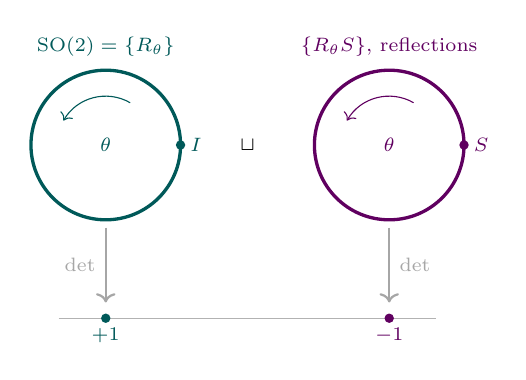
\begin{tikzpicture}
\draw[very thick, teal!70!black] (0.00,0) circle (0.95);
\fill[teal!70!black] (0.95,0) circle (1.7pt) node[anchor=west, font=\scriptsize] {$I$};
\node[teal!70!black, font=\scriptsize] at (0.00,1.25) {$\SO(2) = \{R_\theta\}$};
\draw[->, teal!70!black] (0.00,0) ++(60:0.62) arc (60:150:0.62); \node[font=\scriptsize, teal!70!black] at (0.00,0) {$\theta$};
\draw[very thick, violet!75!black] (3.60,0) circle (0.95);
\fill[violet!75!black] (4.55,0) circle (1.7pt) node[anchor=west, font=\scriptsize] {$S$};
\node[violet!75!black, font=\scriptsize] at (3.60,1.25) {$\{R_\theta S\}$, reflections};
\draw[->, violet!75!black] (3.60,0) ++(60:0.62) arc (60:150:0.62); \node[font=\scriptsize, violet!75!black] at (3.60,0) {$\theta$};
\draw[gray!60] (-0.6,-2.2) -- (4.2,-2.2); \fill[teal!70!black] (0,-2.2) circle (1.7pt) node[below, font=\scriptsize] {$+1$}; \fill[violet!75!black] (3.6,-2.2) circle (1.7pt) node[below, font=\scriptsize] {$-1$};
\draw[->, thick, gray!70] (0,-1.05) -- node[left, font=\scriptsize] {$\det$} (0,-2.0); \draw[->, thick, gray!70] (3.6,-1.05) -- node[right, font=\scriptsize] {$\det$} (3.6,-2.0);
\node[font=\scriptsize] at (1.8,0) {$\sqcup$};
\end{tikzpicture}
\end{center}

$\Ogp(2)$ drawn as two circles. The rotations $R_\theta$ form $\SO(2)$, the matrices of determinant $1$, a circle through $I$. The matrices of determinant $-1$ are the reflections $R_\theta S$ with $S = \mathrm{diag}(1, -1)$ --- if $\det A = -1$ then $AS \in \SO(2)$ --- a second circle. The determinant is continuous with only the values $\pm 1$ on $\Ogp(n)$, so it splits $\Ogp(n)$ into two disjoint open and closed pieces, by the argument that disconnects $\GL(n,\mathbb{R})$ (Proposition~\ref{prop:GL-disconnected}). That each piece is connected, so that $\Ogp(n)$ has exactly two components, is Lee's Proposition~21.34.


\begin{exbox}[Why $\SO(n)$ Is a Proper Subgroup of $\Ogp(n)$]\exlabel{ex:why-n-proper-subgroup-n}
A student asked why one bothers to intersect with $\SL$: does $\Ogp(n)$ not already sit inside $\SL(n)$? No: $\det = \pm 1$, and both signs occur. The reflection
\[
g = \begin{pmatrix} 1 & 0 \\ 0 & -1 \end{pmatrix}
\]
across the $x$-axis is orthogonal ($g^T g = I$) with $\det g = -1$, so $g \in \Ogp(2,\mathbb{R}) \setminus \SO(2,\mathbb{R})$. The same works in every dimension with $\mathrm{diag}(1, \ldots, 1, -1)$.
\end{exbox}
\chapter{Smooth Structures}

% ============================================================================
% Lecture 5 (Fri Sep 11, 2026) -- given by a substitute
% SECTION 7: DIFFERENTIABLE STRUCTURES
% ============================================================================
\section{Differentiable Structures}\label{sec:smooth-structures}

\roadmark{Stage: foundations}{Charts, compatibility, atlases and maximal atlases: what a smooth structure is, for every manifold. The projective spaces get theirs next (\ref{sec:projective-smooth}), then smooth maps (\ref{sec:smooth-maps}).}

\textit{Reference: Lee Ch.\ 1, ``Smooth Structures.'' Lecture 5 was given by a substitute; the transcript is poor, so several steps below are reconstructions and are flagged as such.}

\begin{rembox}[Why This Section]\label{rem:why-this-section-6}
``We want to describe differentiable manifolds. So we take a topological manifold and decorate it a little.'' A topological manifold supports the notion of a \emph{continuous} function and nothing finer; the whole point of a differentiable structure is to make the phrase ``$f$ is differentiable'' meaningful on an abstract space that has no linear structure of its own. Differentiability could mean $C^1, C^2, \ldots$; \textbf{in this course it always means $C^\infty$}, and ``smooth'' and ``differentiable'' are used interchangeably. Everything below was previewed in \S\ref{sub:charts}; the new content is the compatibility requirement and the bookkeeping (atlases, maximal atlases) needed to make the resulting notion independent of choices.
\end{rembox}

\subsection{Smooth Functions Relative to a Chart}

\begin{defbox}[Chart]\deflabel{def:smooth-chart}
Let $M$ be a topological $n$-manifold. As in Definition~\ref{def:chart}, a \textbf{chart} on $M$ is a pair $(U, \varphi)$ where $U \subseteq M$ is open and $\varphi : U \to \varphi(U) \subseteq \mathbb{R}^n$ is a homeomorphism onto an open subset of $\mathbb{R}^n$. The $n$ component functions of $\varphi$ are the \textbf{local coordinates} on $U$.
\leeref{Ch.~1, \emph{Coordinate Charts}}
\end{defbox}

\begin{rembox}\label{rem:smooth-structures}
Requiring $\varphi(U)$ to be open is not an extra condition: by invariance of domain (Theorem~\ref{thm:inv-dim} and the discussion there) a continuous injection from an open subset of $\mathbb{R}^n$ into $\mathbb{R}^n$ is automatically open. The lecture stated only ``$\varphi$ is a homeomorphism onto its image''; we build openness into the definition to avoid invoking a hard theorem.
\end{rembox}

\begin{defbox}[Smooth Function in the Sense of a Chart]\deflabel{def:smooth-in-chart}
Let $(U, \varphi)$ be a chart on $M$. A function $h : U \to \mathbb{R}$ is \textbf{smooth in the sense of $\varphi$} if
\[
h = f \circ \varphi \quad \text{for some smooth } f : \varphi(U) \to \mathbb{R},
\]
where ``smooth'' on the open set $\varphi(U) \subseteq \mathbb{R}^n$ has its usual meaning from multivariable calculus ($C^\infty$: all partial derivatives of all orders exist and are continuous). Since $\varphi$ is a bijection onto $\varphi(U)$, such an $f$ is unique if it exists, namely $f = h \circ \varphi^{-1}$; so the condition may equivalently be stated as
\[
h \text{ is smooth in the sense of } \varphi \iff h \circ \varphi^{-1} : \varphi(U) \to \mathbb{R} \text{ is smooth.}
\]
The first form builds $h$ out of a smooth $f$ and is the one used on the board; the second tests $h$ by pushing it to Euclidean space and is Lee's. They say the same thing, and both are used below.
\leeref{Ch.~2, \emph{Smooth Functions and Smooth Maps}}
\end{defbox}

\begin{rembox}[The Problem This Creates]\label{rem:problem-this-creates}
Definition~\ref{def:smooth-in-chart} depends on $\varphi$, not only on $U$. If a point lies in two chart domains $U$ and $V$, there are \emph{two} notions of smoothness available on $U \cap V$, and nothing so far says they agree. That is the question the rest of the subsection answers: ``you've got a notion of what it means to be differentiable here, and a notion of what it means to be differentiable there --- are they consistent?''
\end{rembox}

\subsection{Compatibility of Charts}\label{sub:compatibility}

\begin{defbox}[Diffeomorphism of Open Subsets of Euclidean Space]\deflabel{def:diffeo-euclidean}
Let $A, B \subseteq \mathbb{R}^n$ be open. A map $F : A \to B$ is a \textbf{diffeomorphism} if it is a bijection and both $F$ and $F^{-1}$ are smooth, and $A$ and $B$ are \textbf{diffeomorphic} if such an $F$ exists. (This is the differentiable analogue of a homeomorphism: a smooth bijection whose inverse is also smooth.)
\leeref{Ch.~1, \emph{Smooth Structures}}
\end{defbox}

\begin{defbox}[Smoothly Compatible Charts]\deflabel{def:compatible}
Two charts $(U, \varphi)$ and $(V, \psi)$ on $M$ are \textbf{$C^\infty$-compatible} if the \textbf{transition function}
\[
\psi \circ \varphi^{-1} : \varphi(U \cap V) \longrightarrow \psi(U \cap V)
\]
is a diffeomorphism in the sense of Definition~\ref{def:diffeo-euclidean}. If $U \cap V = \emptyset$ the condition is vacuous and the charts are compatible.
\leeref{Ch.~1, \emph{Smooth Structures} (``smoothly compatible)}
\end{defbox}

\begin{rembox}\label{rem:smooth-structures-2}
The domain and target are open subsets of $\mathbb{R}^n$, and $\psi \circ \varphi^{-1}$ is automatically a homeomorphism between them --- this is Proposition~\ref{prop:transition-homeo} from \S\ref{sub:charts}, which used nothing but the topological manifold structure. Compatibility asks for the one genuinely new thing: that this homeomorphism and its inverse be $C^\infty$. Note that requiring $\psi\circ\varphi^{-1}$ to be a diffeomorphism is symmetric in the two charts, since $(\psi \circ \varphi^{-1})^{-1} = \varphi \circ \psi^{-1}$.
\end{rembox}


\begin{center}
\begin{tikzcd}[row sep=2.2em, column sep=1.1em]
& U \cap V \subseteq M \arrow[dl, "\varphi"'] \arrow[dr, "\psi"] & \\
\varphi(U \cap V) \subseteq \mathbb{R}^n \arrow[rr, "\psi \circ \varphi^{-1}"'] \arrow[dr, "f"'] & & \psi(U \cap V) \subseteq \mathbb{R}^n \arrow[dl, "g"] \\
& \mathbb{R} &
\end{tikzcd}
\end{center}

The diagram drawn in lecture. The same function on $U \cap V$ is represented downstairs by $f$ in the $\varphi$-coordinates and by $g$ in the $\psi$-coordinates; the upper triangle says $f \circ \varphi = g \circ \psi$, and the lower triangle says $f = g \circ (\psi \circ \varphi^{-1})$. Compatibility is exactly the statement that the horizontal arrow is a diffeomorphism, which is what lets one pass between $f$ and $g$ without leaving the smooth category.

\begin{defbox}[Regularity Classes of Manifolds]\deflabel{def:regularity-classes}
Nothing in Definition~\ref{def:compatible}, or in the definitions of atlases and maximal atlases that follow, is special to $C^\infty$: the regularity of a manifold is imposed \emph{entirely} through its transition functions. Replacing ``smooth'' by another class of maps gives:
\begin{itemize}
    \item a \textbf{$C^k$ manifold}, for a fixed $k \ge 1$: transition functions are $C^k$ with $C^k$ inverses;
    \item a \textbf{real-analytic manifold}: transition functions are real-analytic --- locally given by convergent power series --- with real-analytic inverses;
    \item a \textbf{complex manifold} of complex dimension $n$: charts take values in open subsets of $\mathbb{C}^n$, and transition functions are holomorphic with holomorphic inverses.
\end{itemize}
From here on, unless stated otherwise, everything in this course is $C^\infty$.
\leeref{Ch.~1, \emph{Smooth Structures}}
\end{defbox}

\begin{rembox}[Comparing the Classes]\label{rem:comparing-classes}
Uribe: ``it's all given by what you ask of the transition functions between charts.'' Two cautions on how these classes compare, since the lecture's answer to a student's question was explicitly hedged. First, \emph{lowering $k$ gains nothing}: by a theorem of Whitney, every $C^k$ structure with $k \ge 1$ contains a compatible $C^\infty$ structure, unique up to diffeomorphism, so $C^1$ and $C^\infty$ manifolds are the same objects up to isomorphism. What is genuinely different is $C^0$: there exist topological manifolds carrying \emph{no} smooth structure at all. Second, regularity does matter for \emph{theorems about maps}. Sard's theorem --- that the set of critical values of $F : \mathbb{R}^N \to \mathbb{R}^m$ has measure zero --- requires $F$ to be $C^k$ with $k \ge \max(1, N-m+1)$, and fails for $C^1$ maps otherwise. Real-analytic manifolds are harder to work with for a different reason: $C^\omega$ functions are rigid, so there are no bump functions and hence no partitions of unity, a tool we will rely on constantly.
\end{rembox}

\begin{thmbox}[Compatibility Means the Two Notions Agree]\thmlabel{thm:compat-agree}
Let $(U,\varphi)$ and $(V,\psi)$ be charts on $M$ with $U \cap V \neq \emptyset$. The following are equivalent:
\begin{enumerate}
    \item $(U,\varphi)$ and $(V,\psi)$ are $C^\infty$-compatible;
    \item for every $h : U \cap V \to \mathbb{R}$: $h$ is smooth in the sense of $\varphi$ $\iff$ $h$ is smooth in the sense of $\psi$.
\end{enumerate}
\end{thmbox}

\begin{proof}
\textit{(Not from lecture; filled in. It reconciles two phrasings: Lecture~5 asked that the transition function be a diffeomorphism, Lecture~6 that the transition functions in both directions be smooth.)} Throughout, write $A = \varphi(U \cap V)$ and $B = \psi(U \cap V)$, both open in $\mathbb{R}^n$, and $\tau = \psi \circ \varphi^{-1} : A \to B$, a homeomorphism with inverse $\tau^{-1} = \varphi \circ \psi^{-1}$.

$(1 \Rightarrow 2)$ Suppose $\tau$ is a diffeomorphism, and let $h = f \circ \varphi$ with $f$ smooth on $A$. Put $g = f \circ \tau^{-1}$, smooth on $B$ as a composite of smooth maps. Then
\[
g \circ \psi = f \circ \tau^{-1} \circ \psi = f \circ \varphi \circ \psi^{-1} \circ \psi = f \circ \varphi = h,
\]
so $h$ is smooth in the sense of $\psi$. The converse implication is the same computation with $\tau$ in place of $\tau^{-1}$, using smoothness of $\tau$.

$(2 \Rightarrow 1)$ Apply (2) to the $n$ coordinate functions of $\varphi$. Let $\pi^i : \mathbb{R}^n \to \mathbb{R}$ be the $i$-th coordinate projection and $h_i = \pi^i \circ \varphi$, which is smooth in the sense of $\varphi$ (take $f = \pi^i$). By (2), $h_i = g_i \circ \psi$ for some smooth $g_i$ on $B$, i.e.\ $g_i = h_i \circ \psi^{-1} = \pi^i \circ \varphi \circ \psi^{-1} = \pi^i \circ \tau^{-1}$. So every component of $\tau^{-1}$ is smooth, hence $\tau^{-1}$ is smooth; symmetrically $\tau$ is smooth. Both being continuous bijections already, $\tau$ is a diffeomorphism.
\end{proof}

\begin{rembox}[The Board Version]\label{rem:board-version}
The lecture gave the direction $(1 \Rightarrow 2)$ in the compact form
\[
f = g \circ (\psi \circ \varphi^{-1}), \qquad \text{equivalently} \qquad f \circ \varphi = g \circ \psi,
\]
read as: the same function on $U \cap V$ is represented by $f$ in the $\varphi$-coordinates and by $g$ in the $\psi$-coordinates, and the transition function converts one representative into the other. The converse $(2 \Rightarrow 1)$ was not discussed; it is included because it shows compatibility is not merely \emph{sufficient} for the two notions to agree but \emph{necessary} --- the definition is not an arbitrarily strong choice.
\end{rembox}

\begin{propbox}[Compatibility Is Not an Equivalence Relation]\thmlabel{prop:compat-not-transitive}
$C^\infty$-compatibility of charts is reflexive and symmetric, but not transitive.
\leeref{cf.\ Ch.~1, \emph{Smooth Structures}}
\end{propbox}

\begin{proof}
\textit{(Not from lecture; filled in.)} \emph{Reflexive:} the transition function of a chart with itself is the identity. \emph{Symmetric:} the transition function in the other direction is the inverse diffeomorphism. \emph{Not transitive:} on $M = \mathbb{R}$ let $\varphi_1 = \mathrm{id}$ on $U_1 = \mathbb{R}$, $\varphi_2 = \mathrm{id}$ on $U_2 = (0,\infty)$, and $\varphi_3(t) = t^3$ on $U_3 = \mathbb{R}$. Then $(U_1,\varphi_1)$ and $(U_2,\varphi_2)$ are compatible, and so are $(U_2,\varphi_2)$ and $(U_3,\varphi_3)$, since on $(0,\infty)$ the transition $t \mapsto t^{1/3}$ is smooth with smooth inverse. But $(U_1,\varphi_1)$ and $(U_3,\varphi_3)$ are not: the transition $\varphi_1 \circ \varphi_3^{-1}(t) = t^{1/3}$ fails to be differentiable at $0$.
\end{proof}

\begin{rembox}\label{rem:smooth-structures-3}
This is exactly why Theorem~\ref{thm:maximal-atlas} below cannot be proved by ``collect all charts compatible with a given one.'' The chart $(U_2,\varphi_2)$ is compatible with both of two charts that are incompatible with each other.
\end{rembox}

\subsection{Atlases}

\begin{defbox}[Atlas]\deflabel{def:atlas}
An \textbf{atlas} on a topological $n$-manifold $M$ is a collection $\mathcal{A} = \{(U_i, \varphi_i)\}_{i \in I}$ of pairwise $C^\infty$-compatible charts with $\bigcup_{i} U_i = M$.
\leeref{Ch.~1, \emph{Smooth Structures} (``smooth atlas)}
\end{defbox}

\begin{exbox}[Euclidean Space]\exlabel{ex:atlas-Rn}
$\mathbb{R}^n$ has the one-chart atlas $\{(\mathbb{R}^n, \mathrm{id})\}$. More generally any open $A \subseteq \mathbb{R}^n$ has the atlas $\{(A, \mathrm{id})\}$. A single chart is automatically an atlas: compatibility with itself is the statement that $\mathrm{id}$ is a diffeomorphism.
\leeref{Example 1.22}
\end{exbox}

\begin{exbox}[The Four-Chart Atlas on the Circle]\exlabel{ex:circle-four}
Let $S^1 = \{(x,y) \in \mathbb{R}^2 \mid x^2 + y^2 = 1\}$ and cut it along the axes into four open half-circles, each projected onto the axis it is a graph over:
\[
\begin{array}{llll}
U_1 = \{x > 0\}, & \varphi_1(x,y) = y; \qquad & U_3 = \{x < 0\}, & \varphi_3(x,y) = y;\\
U_2 = \{y > 0\}, & \varphi_2(x,y) = x; & U_4 = \{y < 0\}, & \varphi_4(x,y) = x.
\end{array}
\]
Each $\varphi_i$ is a homeomorphism onto $(-1,1)$, with inverse given by solving $x^2 + y^2 = 1$ for the missing coordinate with the sign determined by the half-circle: e.g.\ $\varphi_1^{-1}(y) = (\sqrt{1-y^2},\, y)$ and $\varphi_4^{-1}(x) = (x,\, -\sqrt{1-x^2})$. The four sets cover $S^1$, so this is an atlas once compatibility is checked.

\emph{Transition functions.} $U_1 \cap U_3 = \emptyset = U_2 \cap U_4$, so those two pairs are vacuously compatible. The four remaining overlaps are the open quadrant arcs, and on each the transition is the map that solves for the other coordinate:
\[
\varphi_2 \circ \varphi_1^{-1}(y) = \sqrt{1-y^2} \ \text{ on } (0,1), \qquad
\varphi_3 \circ \varphi_2^{-1}(x) = \sqrt{1-x^2} \ \text{ on } (-1,0),
\]
\[
\varphi_4 \circ \varphi_3^{-1}(y) = -\sqrt{1-y^2} \ \text{ on } (-1,0), \qquad
\varphi_1 \circ \varphi_4^{-1}(x) = -\sqrt{1-x^2} \ \text{ on } (0,1).
\]
Each is smooth on its (open) domain, because $1 - t^2 > 0$ there, and each is its own inverse up to sign, so all four are diffeomorphisms. Hence $\{(U_i, \varphi_i)\}_{i=1}^4$ is an atlas.
\leeref{Examples 1.4 and 1.31}
\end{exbox}

The board wrote ``$x^2 + y^2 = 0$'' when setting up the first transition function; the equation of the circle is of course $x^2 + y^2 = 1$. The sign in each transition function is dictated by the quadrant --- this is what the lecture meant by ``sometimes the square root is positive, sometimes negative; look at the picture to see where you are.'' Note also that $\sqrt{1-t^2}$ is \emph{not} smooth at $t = \pm 1$; it does not need to be, because those values are not in the domain of any transition function. Cutting at the axes is exactly what keeps the bad points out.


\begin{center}
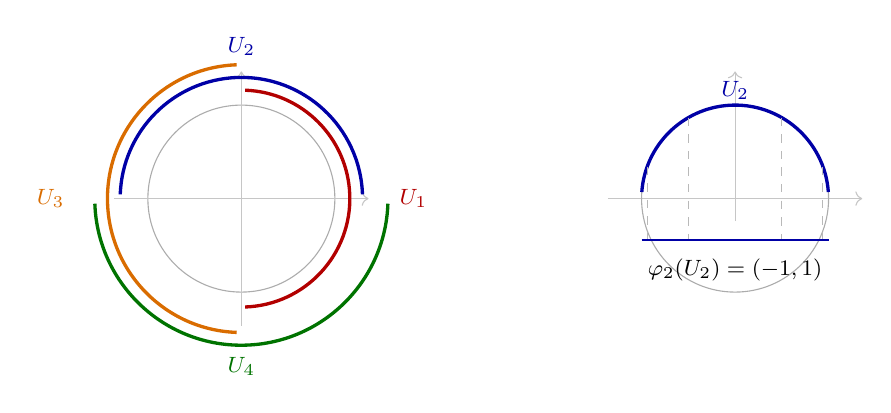
\begin{tikzpicture}[scale=0.95]
\draw[gray!65] (0,0) circle (1.25);
\draw[gray!45,->] (-1.7,0) -- (1.7,0); \draw[gray!45,->] (0,-1.7) -- (0,1.7);
\draw[red!70!black,very thick] (-88:1.45) arc (-88:88:1.45);
\draw[blue!65!black,very thick] (2:1.62) arc (2:178:1.62);
\draw[orange!85!black,very thick] (92:1.79) arc (92:268:1.79);
\draw[green!45!black,very thick] (182:1.96) arc (182:358:1.96);
\node[red!70!black,font=\footnotesize] at (2.3,0) {$U_1$};
\node[blue!65!black,font=\footnotesize] at (0,2.04) {$U_2$};
\node[orange!85!black,font=\footnotesize] at (-2.55,0) {$U_3$};
\node[green!45!black,font=\footnotesize] at (0,-2.24) {$U_4$};
\begin{scope}[xshift=6.6cm]
\draw[gray!45,->] (-1.7,0) -- (1.7,0); \draw[gray!45,->] (0,-0.3) -- (0,1.7);
\draw[gray!65] (0,0) circle (1.25);
\draw[blue!65!black,very thick] (4:1.25) arc (4:176:1.25);
\foreach \a in {20,60,120,160} { \draw[dashed,gray!55] (\a:1.25) -- ({1.25*cos(\a)},-0.55); }
\draw[blue!65!black,thick] (-1.25,-0.55) -- (1.25,-0.55);
\node[font=\footnotesize,anchor=north] at (0,-0.68) {$\varphi_2(U_2)=(-1,1)$};
\node[blue!65!black,font=\footnotesize] at (0,1.45) {$U_2$};
\end{scope}
\end{tikzpicture}
\end{center}

\emph{Left:} the four half-circles, drawn at staggered radii so the overlaps are visible. $U_1$ and $U_3$ never meet, nor do $U_2$ and $U_4$; the four nonempty overlaps are the open quadrant arcs, where consecutive colors run alongside each other. \emph{Right:} the chart $\varphi_2$ on the upper half-circle is vertical projection onto the $x$-axis, a homeomorphism onto $(-1,1)$. Each of the four charts is a projection onto the axis its half-circle is a graph over, which is why the transition functions come out as $\pm\sqrt{1-t^2}$.

\begin{propbox}[The Circle Needs More Than One Chart]\thmlabel{prop:circle-no-global-chart}
There is no atlas on $S^1$ consisting of a single chart; that is, $S^1$ is not homeomorphic to an open subset of $\mathbb{R}$.
\end{propbox}

\begin{proof}
\textit{(Lecture~5 gave the reason: an open subset of $\mathbb{R}$ cannot be homeomorphic to the compact circle; filled in.)} Suppose $\varphi : S^1 \to \varphi(S^1) \subseteq \mathbb{R}$ were such a chart. Then $\varphi(S^1)$ is open by Definition~\ref{def:smooth-chart}, and compact as the continuous image of the compact space $S^1$ (Proposition~\ref{fact:compact}(1) gives compactness of $S^1$, closed and bounded in $\mathbb{R}^2$; (2) gives compactness of the image). A compact subset of the Hausdorff space $\mathbb{R}$ is closed (Proposition~\ref{fact:compact}(4)), so $\varphi(S^1)$ is a nonempty subset of $\mathbb{R}$ that is both open and closed. Since $\mathbb{R}$ is connected, $\varphi(S^1) = \mathbb{R}$ --- which is not compact. Contradiction.
\end{proof}

\begin{rembox}\label{rem:smooth-structures-4}
``It is absolutely essential to break the circle into charts.'' The obstruction is global (compactness), not local: every point of $S^1$ has arbitrarily small neighborhoods that are perfectly good chart domains. A student asked which open sets can serve; the answer is the next proposition.
\end{rembox}

\begin{exbox}[Stereographic Atlas on the Circle]\exlabel{ex:circle-stereo}
Let $N = (0,1)$ and $S = (0,-1)$ be the north and south poles. For $P \in S^1 \setminus \{N\}$, the line through $N$ and $P$ meets the $x$-axis in exactly one point; sending $P$ to that point defines
\[
\sigma_N : S^1 \setminus \{N\} \to \mathbb{R}, \quad \sigma_N(x,y) = \frac{x}{1-y}, \qquad
\sigma_S : S^1 \setminus \{S\} \to \mathbb{R}, \quad \sigma_S(x,y) = \frac{x}{1+y}.
\]
Both are homeomorphisms onto $\mathbb{R}$, with $\sigma_N^{-1}(u) = \left( \frac{2u}{u^2+1},\, \frac{u^2-1}{u^2+1} \right)$. The two domains cover $S^1$, their intersection is $S^1 \setminus \{N, S\}$, and
\[
\sigma_S \circ \sigma_N^{-1}(u) = \frac{2u/(u^2+1)}{1 + (u^2-1)/(u^2+1)} = \frac{2u}{2u^2} = \frac{1}{u},
\]
a diffeomorphism of $\mathbb{R} \setminus \{0\}$ onto itself. So $\{(S^1 \setminus \{N\}, \sigma_N), (S^1 \setminus \{S\}, \sigma_S)\}$ is an atlas with only two charts. (``It is going to be a rational function'': here $u \mapsto 1/u$.) Consistently with Proposition~\ref{prop:circle-no-global-chart}, two is the minimum.
\leeref{Problem 1-7}
\end{exbox}


\begin{center}
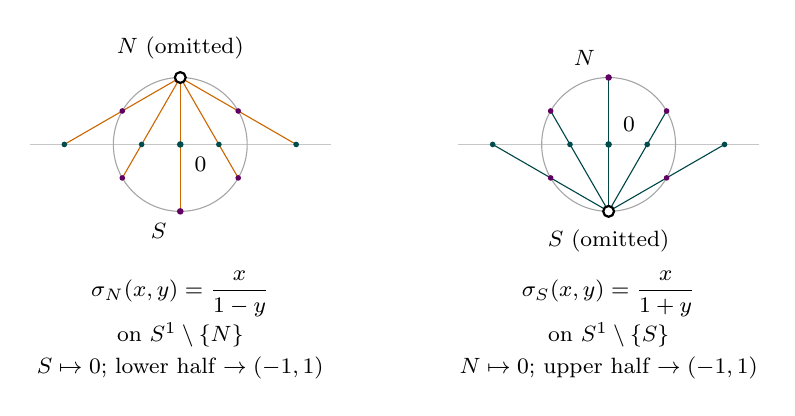
\begin{tikzpicture}[scale=0.85]
\draw[gray!45] (-2.25,0) -- (2.25,0);
\draw[gray!70] (0,0) circle (1);
\draw[orange!80!black,thin] (0,1) -- (0,0) -- (0,-1);
\foreach \a/\u in {30/1.732, 150/-1.732, -30/0.577, 210/-0.577} {
  \draw[orange!80!black,thin] (0,1) -- (\u,0) -- (\a:1);
  \fill[violet!75!black] (\a:1) circle (1.2pt);
  \fill[teal!60!black] (\u,0) circle (1.2pt); }
\fill[violet!75!black] (0,-1) circle (1.4pt);
\fill[teal!60!black] (0,0) circle (1.4pt);
\draw[fill=white,thick] (0,1) circle (2.3pt);
\node[font=\footnotesize,anchor=south] at (0,1.13) {$N$ (omitted)};
\node[font=\footnotesize,anchor=north east] at (-0.06,-1.04) {$S$};
\node[font=\footnotesize,anchor=north west] at (0.07,-0.04) {$0$};
\node[font=\footnotesize,align=center,anchor=north] at (0,-1.75) {$\sigma_N(x,y)=\dfrac{x}{1-y}$\\[1pt] on $S^1\setminus\{N\}$\\[2pt] $S\mapsto0$; lower half $\to(-1,1)$};
\begin{scope}[shift={(6.4,0)}]
\draw[gray!45] (-2.25,0) -- (2.25,0);
\draw[gray!70] (0,0) circle (1);
\draw[teal!55!black,thin] (0,-1) -- (0,0) -- (0,1);
\foreach \a/\u in {30/0.577, 150/-0.577, -30/1.732, 210/-1.732} {
  \draw[teal!55!black,thin] (0,-1) -- (\u,0) -- (\a:1);
  \fill[violet!75!black] (\a:1) circle (1.2pt);
  \fill[teal!60!black] (\u,0) circle (1.2pt); }
\fill[violet!75!black] (0,1) circle (1.4pt);
\fill[teal!60!black] (0,0) circle (1.4pt);
\draw[fill=white,thick] (0,-1) circle (2.3pt);
\node[font=\footnotesize,anchor=north] at (0,-1.13) {$S$ (omitted)};
\node[font=\footnotesize,anchor=south east] at (-0.06,1.04) {$N$};
\node[font=\footnotesize,anchor=south west] at (0.07,0.05) {$0$};
\node[font=\footnotesize,align=center,anchor=north] at (0,-1.75) {$\sigma_S(x,y)=\dfrac{x}{1+y}$\\[1pt] on $S^1\setminus\{S\}$\\[2pt] $N\mapsto0$; upper half $\to(-1,1)$};
\end{scope}
\end{tikzpicture}
\end{center}

The hollow circle marks the pole each chart \emph{omits}: $\sigma_N$ is undefined at $N$, since the line through $N$ and $N$ is not determined, and as $P$ climbs towards $N$ the image $\sigma_N(P)$ runs off to $\pm\infty$. Every other point is hit exactly once, so $\sigma_N$ is a bijection onto all of $\mathbb{R}$.

The vertical ray is the case $P = S$: the line through $N$ and $S$ meets the axis at the origin, so $\sigma_N(S) = 0/(1-(-1)) = 0$, and by symmetry $\sigma_S(N) = 0$. The two charts are mirror images in this respect --- $\sigma_N$ compresses the \emph{lower} half-circle into $(-1,1)$ and throws the upper half outside it, while $\sigma_S$ does the reverse. On the overlap $S^1 \setminus \{N,S\}$ this exchange of inside and outside is exactly the transition function $u \mapsto 1/u$.


\begin{propbox}[Chart Domains on the Circle]\thmlabel{prop:circle-chart-domains}
A connected open subset $V \subseteq S^1$ is the domain of a chart if and only if $V \ne S^1$. Every such $V$ is an open arc, homeomorphic to an open interval.
\end{propbox}

\begin{proof}
\textit{(Not from lecture; filled in.)} If $V \ne S^1$, pick $q \notin V$ and a rotation $\rho$ of $S^1$ with $\rho(q) = N$. The stereographic projection $\sigma_N : S^1 \setminus \{N\} \to \mathbb{R}$ of Example~\ref{ex:circle-stereo} above is a homeomorphism, so $\sigma_N \circ \rho$ maps $V$ homeomorphically onto a connected open subset of $\mathbb{R}$, which is an open interval; this is a chart. Conversely, $S^1$ is not a chart domain, by Proposition~\ref{prop:circle-no-global-chart}.
\end{proof}
\begin{exbox}[Angle Atlas on the Circle]\exlabel{ex:circle-angle}
Parametrize by angle, which cannot be done globally --- the same meta-principle --- so use two overlapping ranges:
\[
\begin{aligned}
U_a &= S^1 \setminus \{(1,0)\}, & \varphi_a(\cos\theta, \sin\theta) &= \theta \in (0, 2\pi); \\
U_b &= S^1 \setminus \{(-1,0)\}, & \varphi_b(\cos\theta, \sin\theta) &= \theta \in (\pi, 3\pi).
\end{aligned}
\]
Here $U_a \cap U_b$ is the union of the open upper and lower half-circles, $\varphi_a(U_a \cap U_b) = (0,\pi) \cup (\pi, 2\pi)$, and
\[
\varphi_b \circ \varphi_a^{-1}(\theta) = \begin{cases} \theta + 2\pi, & \theta \in (0,\pi), \\ \theta, & \theta \in (\pi, 2\pi), \end{cases}
\]
a translation on each component of its domain, hence a diffeomorphism. A parametrization is just the inverse of a chart --- ``putting labels on points'' --- so the two descriptions carry the same information.
\end{exbox}

\begin{rembox}[Three Atlases and One Structure]\label{rem:three-atlases-one-structure}
$S^1$ thus carries at least three different atlases. They are not competing structures: every chart of one is compatible with every chart of another, so they determine the \emph{same} smooth structure. This is proved in Proposition~\ref{prop:circle-atlases-same}, once regular level sets are available. For instance, on the arc where $U_2$ (upper half, coordinate $x$) meets $U_a$ the transition is $\theta \mapsto \cos\theta$ with inverse $x \mapsto \arccos x$, and $\sigma_N \circ \varphi_2^{-1}(x) = x/(1 - \sqrt{1-x^2})$ is smooth on $(-1,0) \cup (0,1)$. ``Which atlas you write down is a matter of convenience'' --- what is intrinsic is the maximal atlas they all generate.
\end{rembox}

\subsection{Maximal Atlases and Smooth Structures}

\begin{defbox}[Compatible Atlases]\deflabel{def:compatible-atlases}
Two atlases $\mathcal{A}, \mathcal{A}'$ on $M$ are \textbf{$C^\infty$-compatible} if every chart of $\mathcal{A}$ is $C^\infty$-compatible with every chart of $\mathcal{A}'$; equivalently, if $\mathcal{A} \cup \mathcal{A}'$ is again an atlas.
\leeref{Proposition 1.17(b)}
\end{defbox}

\begin{defbox}[Maximal Atlas]\deflabel{def:maximal-atlas}
An atlas $\mathcal{A}$ is \textbf{maximal} if every chart compatible with all the charts of $\mathcal{A}$ already belongs to $\mathcal{A}$. Equivalently, $\mathcal{A}$ is contained in no strictly larger atlas.
\leeref{Ch.~1, \emph{Smooth Structures}}
\end{defbox}

\begin{thmbox}[Every Atlas Lies in a Unique Maximal Atlas]\thmlabel{thm:maximal-atlas}
Let $\mathcal{A}$ be an atlas on $M$ and let
\[
\overline{\mathcal{A}} = \{\, (V, \psi) \text{ a chart on } M \mid (V,\psi) \text{ is compatible with every chart of } \mathcal{A} \,\}.
\]
Then $\overline{\mathcal{A}}$ is the unique maximal atlas containing $\mathcal{A}$. Consequently two atlases are compatible if and only if they are contained in the same maximal atlas.
\leeref{Proposition 1.17(a)}
\end{thmbox}

\begin{proof}
\emph{$\overline{\mathcal{A}}$ is an atlas.} \textit{(Lecture~6's sketch, completed.)} It contains $\mathcal{A}$ (whose charts are pairwise compatible), so its domains cover $M$. The content is that any two of its charts are compatible with \emph{each other} --- which does not follow formally, compatibility not being transitive. Let $(V,\psi), (W,\chi) \in \overline{\mathcal{A}}$; we show $\chi \circ \psi^{-1}$ is smooth on $\psi(V \cap W)$. Smoothness is a local property, so it suffices to prove it near each point $\psi(p)$, $p \in V \cap W$. Choose $(U,\varphi) \in \mathcal{A}$ with $p \in U$, possible since $\mathcal{A}$ covers $M$. On the open set $\psi(U \cap V \cap W) \ni \psi(p)$,
\[
\chi \circ \psi^{-1} = (\chi \circ \varphi^{-1}) \circ (\varphi \circ \psi^{-1}),
\]
and both factors are smooth because $(U,\varphi)$ is compatible with each of $(W,\chi)$ and $(V,\psi)$ --- this factorization is the ``little bit of diagram chasing'' of the lecture. Hence $\chi \circ \psi^{-1}$ is smooth near $\psi(p)$. As $p$ was arbitrary it is smooth on all of $\psi(V\cap W)$, and exchanging the roles of the two charts gives smoothness of the inverse.

\emph{$\overline{\mathcal{A}}$ is maximal.} If a chart $(V,\psi)$ is compatible with every chart of $\overline{\mathcal{A}}$, then in particular with every chart of $\mathcal{A} \subseteq \overline{\mathcal{A}}$, so $(V,\psi) \in \overline{\mathcal{A}}$ by definition.

\emph{Uniqueness.} Let $\mathcal{M}$ be any maximal atlas with $\mathcal{A} \subseteq \mathcal{M}$. If $(V,\psi) \in \mathcal{M}$ then it is compatible with every chart of $\mathcal{M}$, hence with every chart of $\mathcal{A}$, so $(V,\psi) \in \overline{\mathcal{A}}$; thus $\mathcal{M} \subseteq \overline{\mathcal{A}}$. Since $\overline{\mathcal{A}}$ is an atlas containing $\mathcal{M}$ and $\mathcal{M}$ is maximal, $\mathcal{M} = \overline{\mathcal{A}}$.
\end{proof}

Lecture~5 argued uniqueness only (``anything in one is contained in the other, so they are equal''), taking for granted that the collection of all compatible charts is an atlas. Lecture~6 returned to the lemma: Uribe defined $\overline{\mathcal{A}}$ as above, called maximality ``not that hard'' and the atlas property ``more substantial'', and sketched it --- a point of the overlap lies in some chart of $\mathcal{A}$, compatible with both charts, ``and then you have to do a little bit of diagram chasing'' --- skipping the details for time. The proof above completes that sketch. That step is the one with content, and the remark on non-transitivity above shows it really needs the mediating chart $(U,\varphi) \in \mathcal{A}$: without an atlas to pass through, pairwise compatibility with a single chart proves nothing. Compare Lee, Proposition 1.17.

\begin{defbox}[Smooth Manifold Structure]\deflabel{def:smooth-structure}
A \textbf{differentiable (smooth) structure} on a topological manifold $M$ is a maximal atlas $\mathcal{A}$ on $M$. A \textbf{smooth manifold} is a pair $\mathcal{M} = (M, \mathcal{A})$. By Theorem~\ref{thm:maximal-atlas}, specifying any atlas specifies a smooth structure, and two atlases specify the same structure exactly when they are compatible.
\leeref{Ch.~1, \emph{Smooth Structures}}
\end{defbox}

\begin{rembox}[On the Connectedness Assumption]\label{rem:connectedness-assumption}
The board wrote ``let $M$ be a topological manifold (connected).'' Nothing in this section uses connectedness, and the definitions above are stated without it. It is a harmless convenience --- with $n$ fixed in advance (Definition~\ref{def:manifold}) the dimension is already constant --- and it can be dropped. It does matter under the convention where $n$ is allowed to vary with the point (Corollary~\ref{cor:dim-loc-const}).
\end{rembox}

% ============================================================================
% SECTION: PROJECTIVE SPACES AS SMOOTH MANIFOLDS
% ============================================================================

\section{Projective Spaces as Smooth Manifolds}\label{sec:projective-smooth}\label{sub:projective-atlas}

\roadmark{Stage: foundations}{The quotient-built manifolds get their smooth structures from atlases written down by hand: $\mathbb{CP}^n$, with holomorphic transition functions.}

The projections $S^n \to \mathbb{RP}^n$ and $S^{2n+1} \to \mathbb{CP}^n$ through the course: the second is the quotient map that defines $\mathbb{CP}^n$ in Section~\ref{sec:ex-cpn}, an orbit map in Example~\ref{ex:cpn-orbit}; the first is the quotient map of Proposition~\ref{prop:rpn-topologies}, and both are read in the standard atlases of Section~\ref{sec:projective-smooth}; Section~\ref{sec:ex-hopf} shows the first is a two-to-one local diffeomorphism and the second a submersion and a fibration, the Hopf fibration, with local but no global sections; and for $n = 3$ the first returns as $S^3 = \mathrm{SU}(2) \to \SO(3) \cong \mathbb{RP}^3$ in Theorem~\ref{thm:double-cover}.


\textit{Assignment 2, Problem 2(b)--(c). This completes the construction begun in \S\ref{sub:cpn}: there $\mathbb{CP}^n$ was shown to be compact, Hausdorff and second countable; here it acquires charts, and the charts turn out to be smoothly --- indeed holomorphically --- compatible.}

\begin{defbox}[Homogeneous Coordinates]\deflabel{def:homogeneous-coords}
For $\vec z = (z_0, \ldots, z_n) \in \mathbb{C}^{n+1} \setminus \{0\}$, write $[z_0 : z_1 : \cdots : z_n] \in \mathbb{CP}^n$ for the complex line through $\vec z$ (Proposition~\ref{prop:cpn-lines}). The $z_i$ are \textbf{homogeneous coordinates} of that point; they are determined only up to a common nonzero factor, $[\vec z] = [\lambda\vec z]$ for every $\lambda \in \mathbb{C}^\times$.
\leeref{Problem 1-9}
\end{defbox}

Let $\pi : \mathbb{C}^{n+1} \setminus \{0\} \to \mathbb{CP}^n$ be the projection $\vec z \mapsto [\vec z]$ of Proposition~\ref{prop:cpn-lines}. Throughout, $\mathbb{C}^m \cong \mathbb{R}^{2m}$ by Definition~\ref{def:complex-groups}.

\begin{defbox}[The Standard Charts on $\mathbb{CP}^n$]\deflabel{def:cpn-charts}
For $i \in \{0, 1, \ldots, n\}$ let
\[
U_i = \{\, [\vec z] \in \mathbb{CP}^n \mid z_i \neq 0 \,\},
\qquad
\varphi_i : U_i \to \mathbb{C}^n, \quad \varphi_i\big([z_0 : \cdots : z_n]\big) = \Big( \frac{z_k}{z_i} \Big)_{k \neq i}.
\]
It is convenient to index the $n$ entries of a point of the target by $\{0,\ldots,n\} \setminus \{i\}$ rather than by $\{1,\ldots,n\}$; this only relabels the slots. Equivalently $U_i = \{\ell \mid \ell \cap \{z_i = 0\} = \{0\}\}$: the lines not lying in the $i$-th coordinate hyperplane.
\leeref{Problem 1-9}
\end{defbox}

\begin{propbox}[Each $\varphi_i$ Is a Chart]\thmlabel{prop:cpn-chart}
$U_i$ is open in $\mathbb{CP}^n$, and $\varphi_i$ is a well-defined homeomorphism of $U_i$ onto $\mathbb{C}^n \cong \mathbb{R}^{2n}$, with inverse
\[
\varphi_i^{-1}(\vec w) = [\, w_0 : \cdots : w_{i-1} : 1 : w_{i+1} : \cdots : w_n \,] \qquad \text{($1$ in slot $i$).}
\]
\leeref{Problem 1-9}
\end{propbox}

\begin{center}
\begin{tikzcd}[row sep=4em, column sep=6em]
\pi^{-1}(U_i) \arrow[r, shift left=0.8ex, "\tilde\varphi_i"] \arrow[d, "p"'] & \mathbb{C}^n \arrow[l, shift left=0.8ex, "s_i"] \arrow[dl, shift left=1.1ex, "\psi_i", pos=0.45] \\
U_i \arrow[ur, shift left=1.1ex, "\varphi_i", pos=0.45] &
\end{tikzcd}
\end{center}

Here $p = \pi|_{\pi^{-1}(U_i)}$, the map $\tilde\varphi_i(\vec z) = (z_k/z_i)_{k\neq i}$ divides by the $i$-th coordinate, and $s_i$ inserts a $1$ in slot $i$. The pattern of Proposition~\ref{prop:cpn-lines} recurs: upstairs $\tilde\varphi_i \circ s_i = \mathrm{id}$ but $s_i \circ \tilde\varphi_i$ rescales $\vec z$ to $\vec z/z_i$; downstairs $\varphi_i$ and $\psi_i = p \circ s_i$ are mutually inverse. The triangle $\varphi_i \circ p = \tilde\varphi_i$ is where the universal property is applied --- to $p$, not to $\pi$, which is the job of Lemma~\ref{lem:quotient-restrict}.


\begin{proof}
\emph{$U_i$ is well defined and open.} Every nonzero vector on a line $\ell$ is a scalar multiple $\lambda\vec z$, $\lambda \neq 0$, of any one of them, and $(\lambda\vec z)_i = \lambda z_i$; so ``$z_i \neq 0$'' holds for one representative iff for all. Hence
\[
\pi^{-1}(U_i) = \{\, \vec z \in \mathbb{C}^{n+1}\setminus\{0\} \mid z_i \neq 0 \,\},
\]
whose complement in $\mathbb{C}^{n+1}\setminus\{0\}$ is $H_i \setminus \{0\}$ with $H_i = \{z_i = 0\}$ a linear subspace, hence closed. So $\pi^{-1}(U_i)$ is open and, by the definition of the quotient topology, $U_i$ is open.

\emph{$\varphi_i$ is well defined.} For $\lambda \in \mathbb{C}^\times$ and $k \neq i$, $(\lambda z_k)/(\lambda z_i) = z_k/z_i$.

\emph{Bijectivity.} Let $s_i : \mathbb{C}^n \to \mathbb{C}^{n+1}\setminus\{0\}$ insert $1$ in slot $i$, and $\psi_i = \pi \circ s_i$. Then $\varphi_i(\psi_i(\vec w)) = \vec w$, since the representative $s_i(\vec w)$ has $i$-th entry $1$. Conversely, for $\ell = [\vec z] \in U_i$ the vector $\vec z/z_i$ represents $\ell$, has $i$-th entry $1$, and has remaining entries $\varphi_i(\ell)$; so $\psi_i(\varphi_i(\ell)) = \ell$. Thus $\psi_i = \varphi_i^{-1}$.

\emph{$\varphi_i$ is continuous.} By Lemma~\ref{lem:quotient-restrict}, since $\pi$ is a quotient map and $U_i$ is open, the restriction $p = \pi|_{\pi^{-1}(U_i)} : \pi^{-1}(U_i) \to U_i$ is a quotient map. The map $\tilde\varphi_i(\vec z) = (z_k/z_i)_{k\neq i}$ on $\pi^{-1}(U_i)$ is continuous (each component is a quotient of continuous functions with nonvanishing denominator) and constant on the fibres of $p$ by well-definedness. By the universal property (Theorem~\ref{thm:univ-quotient-full}) it descends to a continuous map on $U_i$, which is $\varphi_i$.

\emph{$\varphi_i^{-1}$ is continuous.} $\psi_i = \pi \circ s_i$, and $s_i$ is continuous (its components are coordinates or the constant $1$).
\end{proof}

\begin{rembox}\label{rem:smooth-structures-5}
This is where Lemma~\ref{lem:quotient-restrict} earns its place. The map $\tilde\varphi_i$ is defined only on the open piece $\pi^{-1}(U_i)$ --- it divides by $z_i$ --- so the universal property cannot be applied to $\pi$ itself; it is applied to $\pi$ restricted over $U_i$, which the lemma guarantees is still a quotient map. Every chart on a quotient space is built by this two-step move.
\end{rembox}

\begin{thmbox}[The Standard Atlas Is Smooth]\thmlabel{thm:cpn-atlas}
$\{(U_i, \varphi_i)\}_{i=0}^n$ is a $C^\infty$ atlas on $\mathbb{CP}^n$. For $i \neq j$,
\[
\varphi_j(U_i \cap U_j) = \{\, \vec w \in \mathbb{C}^n \mid w_i \neq 0 \,\},
\qquad
\big(\varphi_i \circ \varphi_j^{-1}\big)(\vec w) = \Big( \frac{w_k}{w_i} \Big)_{k \neq i},
\]
with the convention $w_j := 1$.
Consequently $\mathbb{CP}^n$ is a compact smooth manifold of (real) dimension $2n$.
\leeref{Problem 1-9}
\end{thmbox}

\begin{center}
\begin{tikzcd}[row sep=3em, column sep=1.4em]
& U_i \cap U_j \arrow[dl, "\varphi_j"'] \arrow[dr, "\varphi_i"] & \\
\{\vec w \mid w_i \neq 0\} \arrow[rr, "\varphi_i \circ \varphi_j^{-1}"'] & & \{\vec w \mid w_j \neq 0\}
\end{tikzcd}
\end{center}

The compatibility triangle of \S\ref{sub:compatibility} for two standard charts. The overlap lives upstairs in $\mathbb{CP}^n$; its two images downstairs are open subsets of $\mathbb{C}^n$, each cut out by one nonvanishing coordinate, and the bottom arrow is the transition function computed below.


\begin{proof}
\emph{Cover.} If $\vec z \neq 0$ some $z_i \neq 0$, so $[\vec z] \in U_i$.

\emph{Domains.} By Proposition~\ref{prop:cpn-chart}, $\varphi_j^{-1}(\vec w)$ is represented by $s_j(\vec w)$, whose $j$-th entry is $1$ and whose $k$-th entry is $w_k$ for $k \neq j$. It lies in $U_i$ iff its $i$-th entry is nonzero, i.e.\ (as $i \neq j$) iff $w_i \neq 0$. This set is open, being the preimage of $\mathbb{C}\setminus\{0\}$ under the continuous coordinate $\vec w \mapsto w_i$.

\emph{Transition functions.} Applying $\varphi_i$ to the representative $s_j(\vec w)$ divides every entry by its $i$-th entry $w_i$ and deletes slot $i$, giving the displayed formula; in particular the entry in slot $j$ is $1/w_i$. Each entry $w_k/w_i$ is a quotient of polynomials with denominator nonvanishing on the domain. In real coordinates, writing $w_k = a_k + \mathrm{i}\,b_k$ (with $\mathrm{i}$ the imaginary unit, to distinguish it from the index $i$),
\[
\frac{w_k}{w_i} = \frac{w_k\,\overline{w_i}}{|w_i|^2} = \frac{a_k a_i + b_k b_i}{a_i^2 + b_i^2} + \mathrm{i}\,\frac{b_k a_i - a_k b_i}{a_i^2 + b_i^2},
\]
so both real components are rational functions with nonvanishing denominator $|w_i|^2$, hence $C^\infty$. Exchanging $i$ and $j$ gives the inverse transition, also $C^\infty$; so any two charts are compatible.

\emph{Conclusion.} The $U_i$ are open and cover, the $\varphi_i$ are homeomorphisms onto the open set $\mathbb{C}^n \cong \mathbb{R}^{2n}$, and all transitions are diffeomorphisms: this is a smooth atlas, determining a smooth structure by Theorem~\ref{thm:maximal-atlas}. Hausdorffness, second countability and compactness are Propositions~\ref{prop:cpn} and \ref{prop:cpn-compact}.
\end{proof}

\begin{corbox}[$\mathbb{CP}^n$ Is a Complex Manifold]\thmlabel{cor:cpn-complex}
The transition functions of the standard atlas are holomorphic. Hence $\mathbb{CP}^n$ is a complex manifold of complex dimension $n$, in the sense of Definition~\ref{def:regularity-classes}.
\end{corbox}

\begin{proof}
\textit{(Not from lecture; filled in.)} Each component $\vec w \mapsto w_k/w_i$ of a transition function (Theorem~\ref{thm:cpn-atlas}) is a quotient of complex polynomials with denominator nonvanishing on the domain, hence holomorphic.
\end{proof}

\begin{propbox}[$\mathbb{CP}^1$ Is the Riemann Sphere]\thmlabel{prop:cp1-sphere}
$\mathbb{CP}^1$ is homeomorphic to $S^2$.
\leeref{Problem 4-5(b)}
\end{propbox}

\begin{proof}
\textit{(Not from lecture; filled in.)} For $(x,y,z) \in S^2$ the identity $(x+iy)(x-iy) = x^2 + y^2 = (1-z)(1+z)$ shows that $[x+iy : 1-z]$, defined when $z \ne 1$, and $[1+z : x-iy]$, defined when $z \ne -1$, are the same point of $\mathbb{CP}^1$ wherever both are defined. So there is a well-defined map $\Phi : S^2 \to \mathbb{CP}^1$, continuous on each of the two open sets $\{z \ne 1\}$ and $\{z \ne -1\}$ covering $S^2$, hence continuous. On $S^2 \setminus \{N\}$ it is $p \mapsto [\sigma(p) : 1]$, where $\sigma(x,y,z) = (x+iy)/(1-z)$ is the stereographic projection. This is a bijection onto $\mathbb{C}$, with inverse $w \mapsto \big(2\operatorname{Re} w,\, 2\operatorname{Im} w,\, |w|^2 - 1\big)/(|w|^2+1)$. So $\Phi$ maps $S^2 \setminus \{N\}$ bijectively onto $U_1 = \{[w : 1]\}$, and $\Phi(N) = [2 : 0] = [1:0]$ is the one point outside $U_1$. Thus $\Phi$ is a continuous bijection from the compact $S^2$ onto the Hausdorff $\mathbb{CP}^1$ (Proposition~\ref{prop:cpn}), hence a homeomorphism.
\end{proof}

\begin{rembox}\label{rem:smooth-structures-6}
For $n = 1$ there are two standard charts and a single transition function, $w \mapsto 1/w$ on $\mathbb{C} \setminus \{0\}$ --- the complex counterpart of the stereographic transition $u \mapsto 1/u$ of Example~\ref{ex:circle-stereo}.
\end{rembox}

\begin{corbox}[Real Projective Space]\thmlabel{cor:rpn-atlas}
Let $\mathbb{RP}^n = S^n/\{\pm 1\} \cong (\mathbb{R}^{n+1}\setminus\{0\})/\mathbb{R}^\times$, the space of real lines through the origin in $\mathbb{R}^{n+1}$. With $U_i = \{[\vec x] \mid x_i \neq 0\}$ and $\varphi_i([\vec x]) = (x_k/x_i)_{k \neq i}$, the family $\{(U_i, \varphi_i)\}_{i=0}^n$ is a smooth atlas, and $\mathbb{RP}^n$ is a compact smooth manifold of dimension $n$.
\leeref{Example 1.33}
\end{corbox}

\begin{proof}
\textit{(Not from lecture; filled in.)} Every argument of \S\ref{sub:cpn} and of this section goes through verbatim with $\mathbb{R}$, $\mathbb{R}^\times$, $\{\pm1\}$ and $S^n$ in place of $\mathbb{C}$, $\mathbb{C}^\times$, $S^1$ and $S^{2n+1}$: the group $\{\pm 1\}$ is finite, hence compact, and acts on $S^n$ by isometries; the transition maps are the real rational functions $x_k/x_i$. Hausdorffness can alternatively be read off from Corollary~\ref{cor:orbit-T2}.
\end{proof}

\begin{center}
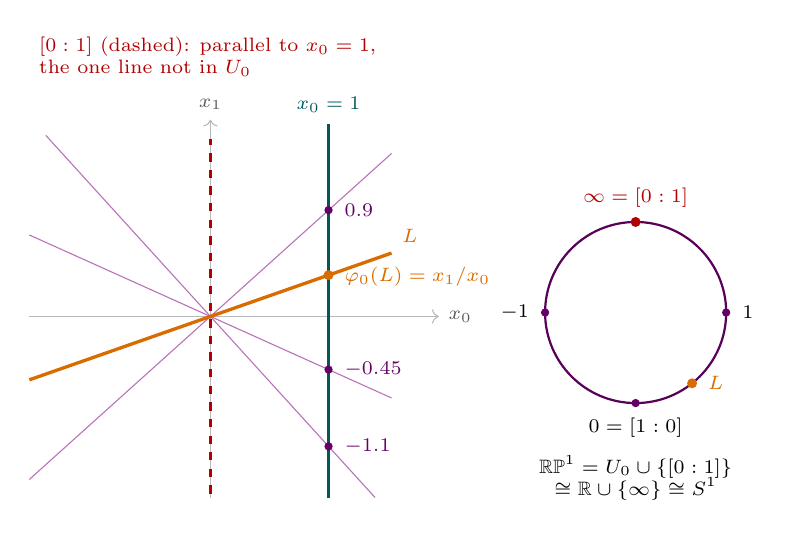
\begin{tikzpicture}
\draw[->, gray!55] (-2.3,0) -- (2.9,0) node[right, font=\scriptsize, text=gray!70!black] {$x_0$}; \draw[->, gray!55] (0,-2.3) -- (0,2.5) node[above, font=\scriptsize, text=gray!70!black] {$x_1$};
\draw[teal!70!black, very thick] (1.50,-2.3) -- (1.50,2.45) node[above, font=\scriptsize] {$x_0 = 1$};
\draw[violet!55] (-2.091,2.300) -- (2.091,-2.300);
\fill[violet!80!black] (1.500,-1.650) circle (1.5pt); \node[font=\scriptsize, anchor=west, text=violet!80!black] at (1.580,-1.650) {$-1.1$};
\draw[violet!55] (-2.300,1.035) -- (2.300,-1.035);
\fill[violet!80!black] (1.500,-0.675) circle (1.5pt); \node[font=\scriptsize, anchor=west, text=violet!80!black] at (1.580,-0.675) {$-0.45$};
\draw[violet!55] (-2.300,-2.070) -- (2.300,2.070);
\fill[violet!80!black] (1.500,1.350) circle (1.5pt); \node[font=\scriptsize, anchor=west, text=violet!80!black] at (1.580,1.350) {$0.9$};
\draw[orange!85!black, very thick] (-2.300,-0.805) -- (2.300,0.805) node[above right, font=\scriptsize] {$L$};
\fill[orange!85!black] (1.500,0.525) circle (1.8pt); \node[font=\scriptsize, anchor=west, text=orange!85!black] at (1.580,0.505) {$\varphi_0(L) = x_1/x_0$};
\draw[red!70!black, very thick, dashed] (0,-2.25) -- (0,2.25); \node[red!70!black, font=\scriptsize, align=left, anchor=west] at (-2.3,3.3) {$[0:1]$ (dashed): parallel to $x_0 = 1$,\\ the one line not in $U_0$};
\draw[thick, violet!70!black] (5.40,0.05) circle (1.15);
\fill[violet!80!black] (5.400,-1.100) circle (1.5pt); \node[font=\scriptsize, anchor=north] at (5.400,-1.160) {$0 = [1:0]$};
\fill[violet!80!black] (6.550,0.050) circle (1.5pt); \node[font=\scriptsize, anchor=west] at (6.630,0.050) {$1$};
\fill[violet!80!black] (4.250,0.050) circle (1.5pt); \node[font=\scriptsize, anchor=east] at (4.170,0.050) {$-1$};
\fill[orange!85!black] (6.117,-0.849) circle (1.8pt); \node[font=\scriptsize, anchor=west, text=orange!85!black] at (6.197,-0.849) {$L$};
\fill[red!70!black] (5.40,1.20) circle (1.8pt); \node[red!70!black, font=\scriptsize, anchor=south] at (5.40,1.26) {$\infty = [0:1]$};
\node[font=\scriptsize, align=center] at (5.40,-2.05) {$\mathbb{RP}^1 = U_0 \cup \{[0:1]\}$\\ $\cong \mathbb{R} \cup \{\infty\} \cong S^1$};
\end{tikzpicture}
\end{center}

The chart $U_0$ of $\mathbb{RP}^1$, drawn in the plane of homogeneous coordinates. A point of $\mathbb{RP}^1$ is a line through the origin. A line $L$ with $x_0 \ne 0$ meets the affine line $x_0 = 1$ in exactly one point, $(1, x_1/x_0)$, and the chart $\varphi_0(L) = x_1/x_0$ records where. The one line with $x_0 = 0$ --- the $x_1$-axis, the point $[0:1]$ --- is parallel to $x_0 = 1$ and never meets it: it is the point at infinity that $U_0$ misses, and the second chart $U_1$ covers it. On the right, $\mathbb{RP}^1$ drawn as a circle, with $U_0$ everything except the top point. In $\mathbb{RP}^n$ the same picture holds with the affine hyperplane $x_0 = 1$ in place of the line.

\begin{propbox}[The Two Topologies on $\mathbb{RP}^n$ Agree]\thmlabel{prop:rpn-topologies}
\begin{enumerate}
    \item Under $[\vec x] \mapsto \mathbb{R}\vec x$, the quotient topology on $\mathbb{RP}^n = S^n/\{\pm1\}$ agrees with the topology of $\Gr_1(\mathbb{R}^{n+1})$ transported from the coset space $\Ogp(n+1)/(\Ogp(1)\times\Ogp(n))$ in \ref{sec:homogeneous}.
    \item $\mathbb{RP}^1$ is homeomorphic to $S^1$.
\end{enumerate}
\leeref{Examples 1.5 and 1.33}
\end{propbox}

\begin{proof}
\textit{(Not from lecture; filled in.)} (1) $\Ogp(n+1)$ acts on $S^n/\{\pm1\}$ by $g \cdot [\vec x] = [g\vec x]$, continuously: the map $\mathrm{id} \times \pi : \Ogp(n+1) \times S^n \to \Ogp(n+1) \times S^n/\{\pm1\}$ is an open continuous surjection, hence a quotient map, and the action descends along it by the universal property. The action is transitive, the coset space is compact, and $S^n/\{\pm1\}$ is Hausdorff, so Theorem~\ref{thm:GH-homeo} identifies $S^n/\{\pm1\}$ homeomorphically with the coset space --- which is precisely the transported topology.

(2) Let $\sigma_N, \sigma_S$ be the stereographic charts of Example~\ref{ex:circle-stereo}, and $\varphi_0, \varphi_1$ the standard charts of $\mathbb{RP}^1$. Define $F = \sigma_N^{-1} \circ \varphi_0$ on $U_0$ and $F = \sigma_S^{-1} \circ \varphi_1$ on $U_1$. On $U_0 \cap U_1$ we have $\varphi_1 = 1/\varphi_0$, and $\sigma_S \circ \sigma_N^{-1}(u) = 1/u$ gives $\sigma_N^{-1}(u) = \sigma_S^{-1}(1/u)$; so the two formulas agree and $F$ is well defined and continuous. It maps $U_0$ bijectively onto $S^1 \setminus \{N\}$, and the one point $[0:1]$ outside $U_0$ to $\sigma_S^{-1}(0) = N$. So $F$ is a continuous bijection from the compact $\mathbb{RP}^1$ onto the Hausdorff $S^1$, hence a homeomorphism. Both transition functions are $u \mapsto 1/u$, and in the charts used $F$ has coordinate representation the identity; so it is even a diffeomorphism, in the sense of Definition~\ref{def:smooth-map} below.
\end{proof}

\begin{center}
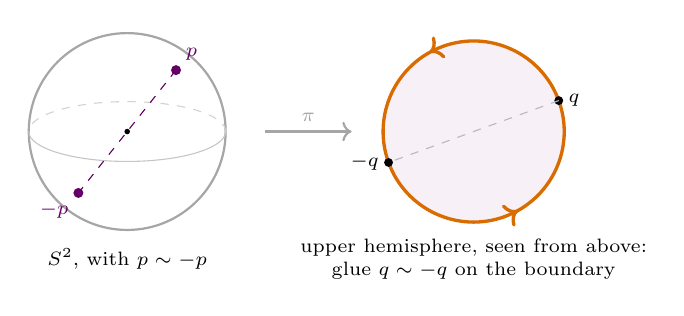
\begin{tikzpicture}
\draw[thick, gray!70] (0,0) circle (1.25); \draw[gray!45] (-1.25,0) arc (180:360:1.25 and 0.38); \draw[gray!35, dashed] (1.25,0) arc (0:180:1.25 and 0.38);
\draw[violet!75!black, dashed] (0.620,0.780) -- (-0.620,-0.780); \fill (0,0) circle (1pt);
\fill[violet!80!black] (0.620,0.780) circle (1.8pt) node[anchor=south west, font=\scriptsize] {$p$}; \fill[violet!80!black] (-0.620,-0.780) circle (1.8pt) node[anchor=north east, font=\scriptsize] {$-p$};
\node[font=\scriptsize] at (0,-1.62) {$S^2$, with $p \sim -p$};
\draw[->, thick, gray!70] (1.75,0) -- node[above, font=\scriptsize] {$\pi$} (2.85,0);
\fill[violet!6] (4.40,0) circle (1.15);
\draw[very thick, orange!85!black, postaction={decorate}, decoration={markings, mark=at position 0.55 with {\arrow{>}}}] (4.40,0) ++(20:1.15) arc (20:200:1.15);
\draw[very thick, orange!85!black, postaction={decorate}, decoration={markings, mark=at position 0.55 with {\arrow{>}}}] (4.40,0) ++(200:1.15) arc (200:380:1.15);
\fill (5.481,0.393) circle (1.6pt) node[anchor=west, font=\scriptsize] {$q$}; \fill (3.319,-0.393) circle (1.6pt) node[anchor=east, font=\scriptsize] {$-q$};
\draw[gray!55, dashed] (5.481,0.393) -- (3.319,-0.393);
\node[font=\scriptsize, align=center] at (4.40,-1.62) {upper hemisphere, seen from above:\\ glue $q \sim -q$ on the boundary};
\end{tikzpicture}
\end{center}

The quotient $S^n \to \mathbb{RP}^n$ of Proposition~\ref{prop:rpn-topologies}, drawn for $n = 2$. A line through the origin meets the sphere in two antipodal points $p$ and $-p$, which $\pi$ identifies. Every line meets the closed upper hemisphere: once if it is not horizontal, and in a pair of antipodal points $q$, $-q$ of the equator if it is. So $\mathbb{RP}^2$ can be pictured as a closed disc with antipodal boundary points glued, as the arrows indicate. For $n = 1$ the same gluing closes a half-circle into a circle, which is $\mathbb{RP}^1 \cong S^1$.

% ============================================================================
% SECTION: SMOOTH FUNCTIONS AND SMOOTH MAPS
% ============================================================================

\section{Smooth Functions and Smooth Maps}\label{sec:smooth-maps}\label{sub:smooth-maps}

\roadmark{Stage: foundations}{With a smooth structure in hand the chart drops out of the phrase ``smooth'': smooth functions, smooth maps, diffeomorphisms and product manifolds.}

Definition~\ref{def:smooth-in-chart} explains what it means for a function to be smooth \emph{in the sense of one chart}. With a smooth structure in hand the chart can be dropped from the phrase. Throughout, $M$ is a smooth manifold with maximal atlas $\mathcal{A}$.

\begin{defbox}[Smooth Chart]\deflabel{def:smooth-chart-M}
Let $M$ be a smooth manifold with maximal atlas $\mathcal{A}$. A \textbf{smooth chart} of $M$ is a chart belonging to $\mathcal{A}$ --- equivalently, by Theorem~\ref{thm:maximal-atlas}, a chart compatible with every chart of some, hence any, atlas generating $\mathcal{A}$.
\leeref{Ch.~1, \emph{Smooth Structures}}
\end{defbox}

\begin{defbox}[Smooth Function on a Manifold]\deflabel{def:smooth-function}
A function $f : M \to \mathbb{R}$ is \textbf{smooth} if for every $p \in M$ there exists a smooth chart $(U,\varphi)$ with $p \in U$ such that
\[
f_\varphi \;:=\; f|_U \circ \varphi^{-1} : \varphi(U) \longrightarrow \mathbb{R}
\]
is smooth in the sense of analysis. (The function $f_\varphi$ is $f$ written in the coordinates of the chart; it is what Definition~\ref{def:smooth-in-chart} called $h \circ \varphi^{-1}$.)
\leeref{Ch.~2, \emph{Smooth Functions and Smooth Maps}}
\end{defbox}

\begin{propbox}[Some Chart Suffices --- Every Chart Then Works]\thmlabel{prop:some-any-function}
If $f : M \to \mathbb{R}$ is smooth, then $f_\psi = f|_V \circ \psi^{-1}$ is smooth for \emph{every} smooth chart $(V,\psi)$ of $M$.
\leeref{Ch.~2, \emph{Smooth Functions and Smooth Maps}}
\end{propbox}

\begin{proof}
\textit{(Stated in lecture, with the proof left to the class; filled in.)} Let $(V,\psi)$ be a smooth chart and $q \in V$; we show $f_\psi$ is smooth on a neighborhood of $\psi(q)$. Since smoothness of a function on an open subset of $\mathbb{R}^n$ is a local property, this suffices. By Definition~\ref{def:smooth-function} there is a smooth chart $(U,\varphi)$ with $q \in U$ and $f_\varphi$ smooth on $\varphi(U)$. Both charts belong to the maximal atlas, so they are compatible, and on the open set $\psi(U \cap V) \ni \psi(q)$,
\[
f_\psi = f \circ \psi^{-1} = \big(f \circ \varphi^{-1}\big) \circ \big(\varphi \circ \psi^{-1}\big) = f_\varphi \circ (\varphi \circ \psi^{-1}),
\]
a composite of the smooth map $f_\varphi$ with the transition function $\varphi \circ \psi^{-1}$, which is smooth by compatibility. Hence $f_\psi$ is smooth near $\psi(q)$.
\end{proof}

\begin{rembox}\label{rem:smooth-structures-7}
The point of logic Uribe stopped to make: the definition says ``there \emph{exists} a chart,'' and the proposition upgrades it to ``\emph{any} chart.'' Without the proposition, smoothness of $f$ would appear to depend on which charts one happened to test it in. The upgrade costs exactly one use of compatibility --- which is what compatibility was designed to buy (Theorem~\ref{thm:compat-agree}). He assigned this as an exercise, not to be collected: ``you have to wrestle with this.''
\end{rembox}

To compare two smooth manifolds one needs smooth \emph{maps} between them.

\begin{defbox}[Smooth Map and Diffeomorphism]\deflabel{def:smooth-map}
Let $(M, \mathcal{A}_M)$ and $(N, \mathcal{A}_N)$ be smooth manifolds of dimensions $m$ and $n$. A map $F : M \to N$ is \textbf{smooth} if it is continuous and for every $p \in M$ there are charts $(U,\varphi) \in \mathcal{A}_M$ with $p \in U$ and $(V,\psi) \in \mathcal{A}_N$ with $F(U) \subseteq V$ such that the \textbf{coordinate representation}
\[
\psi \circ F \circ \varphi^{-1} : \varphi(U) \longrightarrow \psi(V) \subseteq \mathbb{R}^n
\]
is smooth. $F$ is a \textbf{diffeomorphism} if it is a smooth bijection with smooth inverse --- generalizing Definition~\ref{def:diffeo-euclidean}, with which it agrees on open subsets of Euclidean space (Proposition~\ref{prop:diffeo-agree}).
\leeref{Ch.~2, \emph{Smooth Functions and Smooth Maps}}
\end{defbox}


\begin{propbox}[Smoothness of a Map Does Not Depend on the Charts]\thmlabel{prop:smooth-map-charts}
If $F : M \to N$ is smooth, then for \emph{every} pair of smooth charts $(U',\varphi')$ of $M$ and $(V',\psi')$ of $N$ with $F(U') \subseteq V'$, the coordinate representation $\psi' \circ F \circ \varphi'^{-1} : \varphi'(U') \to \psi'(V')$ is smooth. For $N = \mathbb{R}$ with its standard one-chart atlas, Definition~\ref{def:smooth-map} agrees with Definition~\ref{def:smooth-function}.
\leeref{Proposition 2.5}
\end{propbox}

\begin{proof}
\textit{(Not from lecture; filled in.)} Fix $a \in \varphi'(U')$ and put $p = \varphi'^{-1}(a)$. Definition~\ref{def:smooth-map} supplies charts $(U,\varphi)$ at $p$ and $(V,\psi)$ at $F(p)$ with $F(U) \subseteq V$ and $\psi \circ F \circ \varphi^{-1}$ smooth. On the open set $\varphi'(U \cap U') \ni a$,
\[
\psi' \circ F \circ \varphi'^{-1} = (\psi' \circ \psi^{-1}) \circ (\psi \circ F \circ \varphi^{-1}) \circ (\varphi \circ \varphi'^{-1}).
\]
Here $\varphi \circ \varphi'^{-1}$ maps $\varphi'(U \cap U')$ into $\varphi(U \cap U')$, then $F$ maps $U \cap U'$ into $V \cap V'$, and $\psi' \circ \psi^{-1}$ is defined on $\psi(V \cap V')$. The outer factors are transition functions, smooth by compatibility, and the middle one is smooth by hypothesis. So the composite is smooth near $a$, and $a$ was arbitrary. For $N = \mathbb{R}$, taking $\psi = \mathrm{id}$ turns Definition~\ref{def:smooth-map} into Definition~\ref{def:smooth-function}; continuity is automatic there, since $f = f_\varphi \circ \varphi$ near each point.
\end{proof}

\begin{defbox}[Diffeomorphic Manifolds]\deflabel{def:diffeomorphic}
Smooth manifolds $M$ and $N$ are \textbf{diffeomorphic} if there is a diffeomorphism $F : M \to N$. Diffeomorphic manifolds are also called \textbf{isomorphic as smooth manifolds}.
\leeref{Ch.~2, \emph{Diffeomorphisms}}
\end{defbox}

\begin{rembox}\label{rem:smooth-structures-8}
``Diffeomorphic'' is to smooth manifolds what ``homeomorphic'' is to topological spaces: the notion of sameness, under which every smooth property is preserved. No symbol is introduced for it; $\cong$ is already used in these notes for homeomorphisms and linear isomorphisms, so the word is written out.
\end{rembox}

\begin{propbox}[The Two Notions of Diffeomorphism Agree]\thmlabel{prop:diffeo-agree}
Give open sets $A \subseteq \mathbb{R}^m$ and $B \subseteq \mathbb{R}^n$ their standard smooth structures, determined by the charts $(A, \mathrm{id}_A)$ and $(B, \mathrm{id}_B)$. Then a map $F : A \to B$ is smooth in the sense of Definition~\ref{def:smooth-map} if and only if it is smooth in the Euclidean sense. Consequently, for $m = n$, $F$ is a diffeomorphism in the sense of Definition~\ref{def:smooth-map} if and only if it is one in the sense of Definition~\ref{def:diffeo-euclidean}, and $A$ and $B$ are diffeomorphic in the sense of Definition~\ref{def:diffeomorphic} if and only if they are in the sense of Definition~\ref{def:diffeo-euclidean}.
\end{propbox}

\begin{proof}
\textit{(Not from lecture; filled in.)} If $F$ is smooth in the Euclidean sense, it is continuous, and in the charts $(A, \mathrm{id}_A)$ and $(B, \mathrm{id}_B)$ its coordinate representation is $F$ itself, which is smooth. Conversely, suppose $F$ is smooth in the sense of Definition~\ref{def:smooth-map}, and let $p \in A$ with charts $(U, \varphi)$ and $(V, \psi)$ as in that definition. These charts belong to the standard structures, so they are compatible with the identity charts: $\varphi = \varphi \circ \mathrm{id}_A^{-1}$ and $\psi^{-1} = \mathrm{id}_B \circ \psi^{-1}$ are smooth in the Euclidean sense, by Definition~\ref{def:compatible}. Hence on $U$
\[
F = \psi^{-1} \circ \big(\psi \circ F \circ \varphi^{-1}\big) \circ \varphi
\]
is a composite of Euclidean-smooth maps, so $F$ is smooth near $p$. For diffeomorphisms, apply this to $F$ and to $F^{-1}$.
\end{proof}

\begin{rembox}\label{rem:smooth-structures-9}
Not stated in lecture. The word is defined twice because the logic needs it twice: Definition~\ref{def:diffeo-euclidean} must exist before smooth manifolds do, since compatibility of charts is phrased with it, and Definition~\ref{def:smooth-map} is the general notion. The proposition is what licenses using one word for both. A third notion, the \emph{local} diffeomorphism of \ref{sec:special-maps}, is genuinely different; Corollary~\ref{cor:bijective-local-diffeo} relates it to the other two.
\end{rembox}

\begin{lembox}[Composition of Smooth Maps]\thmlabel{lem:composition-smooth}
If $F : M \to N$ and $G : N \to P$ are smooth maps of smooth manifolds, then $G \circ F : M \to P$ is smooth.
\leeref{Proposition 2.10}
\end{lembox}

\begin{proof}
\textit{(Lecture~7: ``something that I would trust ChatGPT to prove without looking at the answer''; filled in.)} $G \circ F$ is continuous as a composite of continuous maps. Fix $p \in M$; we must produce charts at $p$ and at $G(F(p))$ satisfying Definition~\ref{def:smooth-map}. The order of choices matters.

\emph{Step 1: charts for $G$ at $F(p)$.} Since $G$ is smooth, there are smooth charts $(V, \psi)$ of $N$ with $F(p) \in V$ and $(W, \chi)$ of $P$ with $G(V) \subseteq W$ such that $\chi \circ G \circ \psi^{-1}$ is smooth on $\psi(V)$.

\emph{Step 2: a chart for $F$ at $p$ landing inside $V$.} Since $F$ is smooth, there are smooth charts $(U_0, \varphi)$ of $M$ with $p \in U_0$ and $(V_0, \psi_0)$ of $N$ with $F(U_0) \subseteq V_0$ such that $\psi_0 \circ F \circ \varphi^{-1}$ is smooth. The chart $(V_0,\psi_0)$ need not be the $(V,\psi)$ of Step 1, so we adjust. Put $U = U_0 \cap F^{-1}(V)$, an open neighborhood of $p$ since $F$ is continuous, and keep the coordinate map $\varphi|_U$; $(U, \varphi|_U)$ is still a smooth chart (a restriction of one to an open subset). Now $F(U) \subseteq V \cap V_0$, and on $\varphi(U)$
\[
\psi \circ F \circ \varphi^{-1} = (\psi \circ \psi_0^{-1}) \circ (\psi_0 \circ F \circ \varphi^{-1}),
\]
which is smooth: the first factor is a transition function of the maximal atlas of $N$, the second is smooth by the choice of $(U_0,\varphi)$.

\emph{Step 3: compose.} $G \circ F$ maps $U$ into $W$, and on $\varphi(U)$
\[
\chi \circ (G \circ F) \circ \varphi^{-1} = \big(\chi \circ G \circ \psi^{-1}\big) \circ \big(\psi \circ F \circ \varphi^{-1}\big),
\]
a composite of two smooth maps between open subsets of Euclidean spaces (the inner map takes values in $\psi(V)$ because $F(U) \subseteq V$). So $(U, \varphi|_U)$ and $(W, \chi)$ witness the smoothness of $G \circ F$ at $p$.
\end{proof}

\begin{propbox}[Being Diffeomorphic Is an Equivalence Relation]\thmlabel{prop:diffeomorphic-equivalence}
\begin{enumerate}
    \item Being diffeomorphic is an equivalence relation on smooth manifolds.
    \item Diffeomorphic manifolds are homeomorphic.
\end{enumerate}
\leeref{Proposition 2.15}
\end{propbox}

\begin{proof}
\textit{(Not from lecture; filled in.)} (1) \emph{Reflexive:} $\mathrm{id}_M$ is a diffeomorphism, its coordinate representation in any chart $(U,\varphi)$, taken on both sides, being the identity of $\varphi(U)$. \emph{Symmetric:} if $F$ is a diffeomorphism, so is $F^{-1}$, since the definition is symmetric in $F$ and $F^{-1}$. \emph{Transitive:} if $F : M \to N$ and $G : N \to P$ are diffeomorphisms, then $G \circ F$ is smooth by Lemma~\ref{lem:composition-smooth}, and so is its inverse $F^{-1} \circ G^{-1}$. (2) Smooth maps are continuous by Definition~\ref{def:smooth-map}, so a diffeomorphism is a continuous bijection with continuous inverse.
\end{proof}

\begin{rembox}\label{rem:smooth-structures-10}
The converse of (2) is false: Milnor's exotic $7$-spheres are homeomorphic to $S^7$ but not diffeomorphic to it (see the remark after Example~\ref{ex:two-structures-R}). Two further distinctions are worth keeping apart. \emph{Different smooth structures} on one set may still be \emph{diffeomorphic}: in Example~\ref{ex:two-structures-R}, $\mathbb{R}$ and $\widetilde{\mathbb{R}}$ have different maximal atlases, yet $x \mapsto x^3$ is a diffeomorphism between them. And being diffeomorphic is a property of a \emph{pair} of manifolds, while being a diffeomorphism is a property of a \emph{map}: $\mathrm{id} : \mathbb{R} \to \widetilde{\mathbb{R}}$ is not a diffeomorphism even though the two are diffeomorphic.
\end{rembox}

\begin{rembox}\label{rem:smooth-structures-11}
Uribe: ``the composition of smooth maps is smooth is something I would trust ChatGPT to prove without looking at the answer.'' The only content is Step 2 --- the middle charts produced by the two hypotheses need not agree, and one must shrink the domain using continuity of $F$ and then pay one transition function to switch. ``Just compose the two'' skips exactly this.
\end{rembox}


\begin{center}
\begin{tikzcd}[row sep=2.2em, column sep=3.4em]
U \subseteq M \arrow[r, "F"] \arrow[d, "\varphi"'] & V \subseteq N \arrow[d, "\psi"] \\
\varphi(U) \subseteq \mathbb{R}^m \arrow[r, "\psi \circ F \circ \varphi^{-1}"'] & \psi(V) \subseteq \mathbb{R}^n
\end{tikzcd}
\end{center}

The top row is the map one cares about, between spaces where ``smooth'' has no meaning; the bottom row is its coordinate representation, between open subsets of Euclidean spaces where it does. The two vertical arrows are charts, so they are homeomorphisms, and the square commutes by construction. Smoothness of $F$ is \emph{defined} by smoothness of the bottom arrow, and Proposition~\ref{prop:smooth-map-charts} says this does not depend on which charts are used to build it.

\begin{exbox}[Two Smooth Structures on the Real Line]\exlabel{ex:two-structures-R}
Take $M = \mathbb{R}$ as a topological space in both cases, and put
\[
\mathbb{R} = (\mathbb{R}, \{(\mathbb{R}, \varphi)\}), \ \ \varphi = \mathrm{id}; \qquad\qquad
\widetilde{\mathbb{R}} = (\mathbb{R}, \{(\mathbb{R}, \psi)\}), \ \ \psi(p) = \sqrt[3]{p}.
\]
Both $\varphi$ and $\psi$ are homeomorphisms of $\mathbb{R}$ onto $\mathbb{R}$, so each is a legitimate chart (Definition~\ref{def:smooth-chart}), and a one-chart atlas is automatically smooth: the only compatibility to check is of the chart with itself, and the transition function is the identity. By Theorem~\ref{thm:maximal-atlas} each therefore determines a smooth structure.
\leeref{Example 1.23}
\end{exbox}

\begin{proof}[Working out the example]
\textit{(Lecture~5 introduced this example --- the two structures are ``not compatible, but isomorphic'' --- and Lecture~6 returned to it: ``different, but isomorphic. We're going to say diffeomorphic.'' Worked out here.)} \emph{Step 1: the formula of a chart is not a legality condition.} One is tempted to object that $\psi$ ``is not smooth.'' On a bare topological manifold that question is not yet posed: ``smooth'' for a function on $M$ has no meaning until a structure is fixed, and here $\psi$ is what supplies the structure. What makes $\sqrt[3]{\,\cdot\,}$ look illegitimate is a silent comparison against the standard structure of $\mathbb{R}$ --- and that comparison is not part of Definition~\ref{def:smooth-chart}; it is the compatibility question of \S\ref{sub:compatibility}, arriving early and in disguise. Any homeomorphism onto an open set is a chart, whatever its formula. The formula is irrelevant to whether the chart may be written down, and decisive for which structure it produces.

\emph{Step 2: each chart is smooth for its own structure.} By Definition~\ref{def:smooth-in-chart}, a function $h : \mathbb{R} \to \mathbb{R}$ is smooth in the sense of $\psi$ iff $h \circ \psi^{-1}$ is smooth, where $\psi^{-1}(y) = y^3$. Taking $h = \psi$ gives $\psi \circ \psi^{-1} = \mathrm{id}$, which is smooth. So $\sqrt[3]{\,\cdot\,}$ \emph{is} a smooth function on $\widetilde{\mathbb{R}}$. Nothing is special about this chart: the coordinate representation of any chart in its own coordinates is the identity, so every chart of an atlas is smooth for the structure that atlas generates. In the same way $\psi : \widetilde{\mathbb{R}} \to \mathbb{R}$ is a diffeomorphism --- a chart is exactly an identification of its domain with a piece of Euclidean space, carried out in whichever coordinate the chart names.

\emph{Step 3: the two structures are different.} Compatibility is a condition on a \emph{pair} of charts, and it is here that the two disagree. The two transition functions are
\[
\psi \circ \varphi^{-1}(x) = \sqrt[3]{x}, \qquad\qquad \varphi \circ \psi^{-1}(y) = y^3,
\]
and note the asymmetry: the second is smooth, the first is not, since $\tfrac{d}{dx}\sqrt[3]{x} = \tfrac13 x^{-2/3}$ blows up at $x = 0$. Definition~\ref{def:compatible} demands that the transition function be a diffeomorphism, i.e.\ that \emph{both} directions be smooth --- and this example is why: with only one direction required, compatibility would not even be a symmetric relation. So the charts are not compatible, the atlases are not compatible, and the maximal atlases are distinct. Equivalently, in the language of Definition~\ref{def:smooth-map}: the identity map $\mathbb{R} \to \widetilde{\mathbb{R}}$ has coordinate representation $\psi \circ \mathrm{id} \circ \varphi^{-1}(t) = \sqrt[3]{t}$ and is \emph{not} smooth.

\emph{Step 4: which functions are smooth in each.} Smooth in the sense of $\varphi$ means $h \circ \varphi^{-1} = h$ is smooth, so $C^\infty(\mathbb{R})$ is the usual class. Smooth in the sense of $\psi$ means $y \mapsto h(y^3)$ is smooth. Every ordinarily smooth $h$ passes this test, being a composite of smooth maps; and $h = \sqrt[3]{\,\cdot\,}$ passes it while failing the first. Hence
\[
C^\infty(\mathbb{R}) \subsetneq C^\infty(\widetilde{\mathbb{R}}),
\]
a \emph{strict} containment: $\widetilde{\mathbb{R}}$ has more smooth functions than $\mathbb{R}$. The two structures are genuinely different objects, not two names for one.

\emph{Step 5: and yet they are isomorphic.} Define $\Phi : \mathbb{R} \to \widetilde{\mathbb{R}}$, $\Phi(x) = x^3$. Its coordinate representation is $\psi \circ \Phi \circ \varphi^{-1}(t) = \sqrt[3]{t^3} = t$, the identity; the representation of $\Phi^{-1}(y) = \sqrt[3]{y}$ is likewise the identity. So $\Phi$ is a diffeomorphism and $\mathbb{R} \cong \widetilde{\mathbb{R}}$ as smooth manifolds. There is no contradiction with Step 4: the isomorphism is not the identity map, and pullback along $\Phi$ carries $C^\infty(\widetilde{\mathbb{R}})$ bijectively onto $C^\infty(\mathbb{R})$, so a strict containment between isomorphic objects is no more paradoxical here than elsewhere in infinite mathematics.

The moral is that $x$ is merely a \emph{label} for points of $\mathbb{R}$; the structure decides which functions of that label count as smooth, and the two structures decide differently. The identity map respects labels but not structure, while $x \mapsto x^3$ respects structure and scrambles labels.
\end{proof}

\textbf{Transcription note.} The board reads ``Claim: $\exists\,\Phi : \mathbb{R} \to \widetilde{\mathbb{R}}$ which is $C^\infty$, $\Phi(x) = \sqrt[3]{x}$.'' With $\widetilde{\mathbb{R}}$ carrying the chart $\psi = \sqrt[3]{\ \cdot\ }$, that map has coordinate representation $\sqrt[3]{\sqrt[3]{t}} = t^{1/9}$, which is not smooth at $0$; the domain and the formula have been paired the wrong way. The two correct readings are $\Phi : \mathbb{R} \to \widetilde{\mathbb{R}}$ with $\Phi(x) = x^3$ (used above), or the same map read backwards, $\Phi : \widetilde{\mathbb{R}} \to \mathbb{R}$ with $\Phi(x) = \sqrt[3]{x}$. Either way the coordinate representation is the identity, which is what the lecture meant by ``it looks strange, but rewritten in the differentiable coordinate you just get the identity.''

\begin{center}
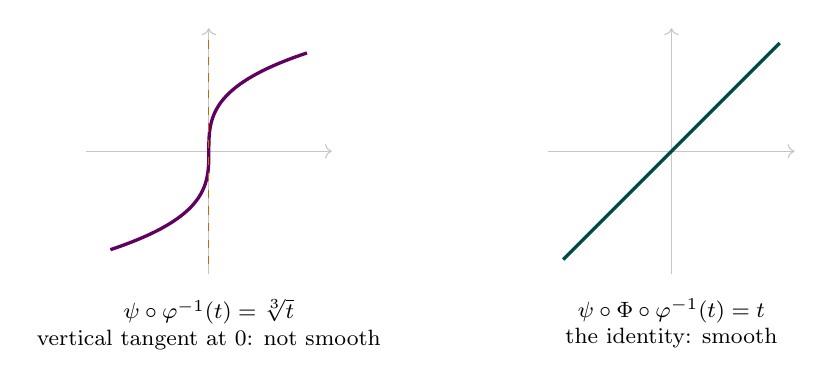
\begin{tikzpicture}[scale=1.25]
\draw[gray!45,->] (-1.25,0)--(1.25,0); \draw[gray!45,->] (0,-1.25)--(0,1.25);
\draw[violet!75!black,very thick,domain=-1:1,samples=90,smooth,variable=\t] plot ({\t*\t*\t},{\t});
\draw[orange!80!black,dashed] (0,-1.15) -- (0,1.15);
\node[font=\footnotesize,align=center,anchor=north] at (0,-1.4) {$\psi\circ\varphi^{-1}(t)=\sqrt[3]{t}$\\ vertical tangent at $0$: not smooth};
\begin{scope}[xshift=4.7cm]
\draw[gray!45,->] (-1.25,0)--(1.25,0); \draw[gray!45,->] (0,-1.25)--(0,1.25);
\draw[teal!60!black,very thick] (-1.1,-1.1) -- (1.1,1.1);
\node[font=\footnotesize,align=center,anchor=north] at (0,-1.4) {$\psi\circ\Phi\circ\varphi^{-1}(t)=t$\\ the identity: smooth};
\end{scope}
\end{tikzpicture}
\end{center}

\begin{propbox}[Transport of Smooth Structure]\thmlabel{prop:transport-structure}
Let $N$ be a smooth $n$-manifold, $X$ a topological space, and $h : X \to N$ a homeomorphism. Then:
\begin{enumerate}
    \item $X$ is a topological $n$-manifold, and $\mathcal{A}_h = \{\, (h^{-1}(V),\ \psi \circ h) \mid (V,\psi) \text{ a smooth chart of } N \,\}$ is a smooth atlas on $X$;
    \item for the smooth structure it determines, $h$ is a diffeomorphism;
    \item it is the \emph{only} smooth structure on $X$ for which $h$ is a diffeomorphism.
\end{enumerate}
\leeref{cf.\ Problem 1-6}
\end{propbox}

\begin{proof}
(1) Hausdorffness and second countability pass through homeomorphisms. Each $\psi \circ h$ is a homeomorphism of the open set $h^{-1}(V)$ onto the open set $\psi(V) \subseteq \mathbb{R}^n$, and these domains cover $X$ because the $V$ cover $N$. Transition functions are $(\psi' \circ h) \circ (\psi \circ h)^{-1} = \psi' \circ \psi^{-1}$, transition functions of $N$, hence smooth.

(2) In the charts $(h^{-1}(V), \psi \circ h)$ of $X$ and $(V, \psi)$ of $N$, the coordinate representation of $h$ is $\psi \circ h \circ (\psi \circ h)^{-1} = \mathrm{id}$, and likewise for $h^{-1}$. Both are continuous, so both are smooth.

(3) Suppose $h$ is a diffeomorphism for some smooth structure $\mathcal{S}$ on $X$, and let $(W, \chi) \in \mathcal{S}$. Then $(\psi \circ h) \circ \chi^{-1} = \psi \circ h \circ \chi^{-1}$ is a coordinate representation of $h$, and $\chi \circ (\psi \circ h)^{-1} = \chi \circ h^{-1} \circ \psi^{-1}$ one of $h^{-1}$; both are smooth by Proposition~\ref{prop:smooth-map-charts}. So every chart of $\mathcal{S}$ is compatible with every chart of $\mathcal{A}_h$, i.e.\ $\mathcal{S}$ lies in the maximal atlas generated by $\mathcal{A}_h$. Since $\mathcal{S}$ is itself maximal, the two coincide (Theorem~\ref{thm:maximal-atlas}).
\end{proof}

\begin{defbox}[Transported Smooth Structure]\deflabel{def:transported}
In the situation of Proposition~\ref{prop:transport-structure}, the smooth structure on $X$ generated by $\mathcal{A}_h$ --- the unique one for which $h$ is a diffeomorphism --- is the smooth structure \textbf{transported} along $h$.
\leeref{cf.\ Problem 1-6}
\end{defbox}

\begin{rembox}\label{rem:smooth-structures-12}
This is the smooth counterpart of Definition~\ref{def:homogeneous-topology}, where a \emph{topology} was transported along a bijection. Here a smooth structure is transported along a homeomorphism: the charts of $N$, precomposed with $h$, become charts of $X$. The structure on $X$ is then ``$N$'s structure, relabelled by $h$'', which is why $h$ is automatically a diffeomorphism.
\end{rembox}

\begin{corbox}[Single-Chart Structures on $\mathbb{R}^n$]\thmlabel{cor:single-chart-Rn}
Let $h : \mathbb{R}^n \to \mathbb{R}^n$ be a homeomorphism, and let $M$ be $\mathbb{R}^n$ with the smooth structure determined by the one-chart atlas $\{(\mathbb{R}^n, h)\}$.
\begin{enumerate}
    \item $\{(\mathbb{R}^n, h)\}$ is a smooth atlas.
    \item $h : M \to \mathbb{R}^n$ is a diffeomorphism onto $\mathbb{R}^n$ with its standard structure. So $M$ is diffeomorphic to standard $\mathbb{R}^n$.
    \item The smooth structure of $M$ \emph{equals} the standard one if and only if $h$ is a diffeomorphism of standard $\mathbb{R}^n$.
\end{enumerate}
\leeref{Example 1.23 and Problem 1-6}
\end{corbox}

\begin{proof}
\textit{(Assignment 3, Problem 1.)} (1) The single domain $\mathbb{R}^n$ covers $M$; $h$ is a homeomorphism onto $h(\mathbb{R}^n) = \mathbb{R}^n$, which is open; and the only transition function is $h \circ h^{-1} = \mathrm{id}_{\mathbb{R}^n}$, which is smooth.

(2) The underlying topological spaces of $M$ and of standard $\mathbb{R}^n$ are the same, so $h$ is a homeomorphism $M \to \mathbb{R}^n$, in particular continuous with continuous inverse $h^{-1}$. In the charts $(\mathbb{R}^n, h)$ of $M$ and $(\mathbb{R}^n, \mathrm{id})$ of standard $\mathbb{R}^n$, the coordinate representation of $h$ is $\mathrm{id} \circ h \circ h^{-1} = \mathrm{id}_{\mathbb{R}^n}$, and that of $h^{-1}$ is $h \circ h^{-1} \circ \mathrm{id}^{-1} = \mathrm{id}_{\mathbb{R}^n}$. Both are smooth, so $h$ is a smooth bijection with smooth inverse. Equivalently, $M$ carries exactly the structure transported along $h$ from standard $\mathbb{R}^n$ (Proposition~\ref{prop:transport-structure}, with the atlas $\{(\mathbb{R}^n, \mathrm{id})\}$ of the target).

(3) The two one-chart atlases determine the same smooth structure if and only if they are compatible (Definition~\ref{def:compatible-atlases}), i.e.\ if and only if $h \circ \mathrm{id}^{-1} = h$ and $\mathrm{id} \circ h^{-1} = h^{-1}$ are both smooth --- that is, if and only if $h$ is a diffeomorphism of standard $\mathbb{R}^n$.
\end{proof}

\begin{center}
\begin{tikzcd}[row sep=3em, column sep=5em]
M = \big(\mathbb{R}^n, \{h\}\big) \arrow[r, "h"] \arrow[d, "h"'] & \mathbb{R}^n_{\text{standard}} \arrow[d, "\mathrm{id}"] \\
\mathbb{R}^n \arrow[r, "\mathrm{id}"'] & \mathbb{R}^n
\end{tikzcd}
\end{center}

The proof of (2) in one square. Upstairs, $h$ is the map between the two manifolds; the vertical arrows are their charts, $h$ on the left and $\mathrm{id}$ on the right. The square commutes, so the coordinate representation along the bottom is the identity: $h$ is as smooth as a map can be, even when, as a map of standard $\mathbb{R}^n$, it is not differentiable at all.

\begin{exbox}[The Real Line with the Cube-Root Chart]\exlabel{ex:cube-root-transport}
For $n = 1$ and $h(x) = \sqrt[3]{x}$, the manifold $M$ is the $\widetilde{\mathbb{R}}$ of Example~\ref{ex:two-structures-R}. By Corollary~\ref{cor:single-chart-Rn}(3) its structure differs from the standard one, since $h$ is not differentiable at $0$. By part (2) it is nevertheless diffeomorphic to standard $\mathbb{R}$, via $h : \widetilde{\mathbb{R}} \to \mathbb{R}$ --- equivalently via $h^{-1}(x) = x^3$ in the other direction, the map $\Phi$ of that example.
\leeref{Example 1.23}
\end{exbox}

\begin{rembox}\label{rem:smooth-structures-13}
Corollary~\ref{cor:single-chart-Rn} produces, from each homeomorphism of $\mathbb{R}^n$ that is not a diffeomorphism --- there are uncountably many --- a smooth structure on $\mathbb{R}^n$ \emph{different} from the standard one. By (2), every one of them is \emph{diffeomorphic} to the standard one. So ``how many smooth structures'' is the wrong question: the right one is how many up to diffeomorphism. It also shows something about the exotic structures of the next remark. An exotic $\mathbb{R}^4$ cannot admit a single chart whose image is all of $\mathbb{R}^4$, since by the argument of (2) that chart would be a diffeomorphism onto standard $\mathbb{R}^4$.
\end{rembox}

\begin{rembox}[Distinct Structures versus Non-Diffeomorphic Manifolds]\label{rem:distinct-structures-versus-non-diffeomorphic}
Example~\ref{ex:two-structures-R} shows that one topological manifold can carry distinct smooth structures --- but that alone is cheap, since pulling any structure back along a homeomorphism that is not a diffeomorphism produces another one, and all of these are diffeomorphic to the original (Proposition~\ref{prop:transport-structure}, Corollary~\ref{cor:single-chart-Rn}). The deep question is whether a topological manifold can carry structures that are \emph{not} diffeomorphic to one another. It can: Milnor found smooth structures on $S^7$ not diffeomorphic to the standard one (1956), and $\mathbb{R}^4$ admits uncountably many pairwise non-diffeomorphic structures, the first produced by combining Freedman's topological classification with Donaldson's gauge theory, the uncountable family by Taubes. By contrast $\mathbb{R}^n$ for $n \neq 4$ admits exactly one up to diffeomorphism --- a result of Stallings for $n \ge 5$ and of Rad\'o and Moise for $n \le 3$, not of Donaldson, to whom the lecture attributed it. All of this is far outside the course, but it is why the definitions above are made so carefully.
\end{rembox}

\subsection{Product Manifolds}\label{sub:product-manifolds}

\textit{Lecture 11 (Fri Sep 25). The product of two smooth manifolds is a smooth manifold, with the products of charts as an atlas; its tangent spaces are treated in \ref{sub:tangent-products}.}

\begin{propbox}[The Product Smooth Structure]\thmlabel{prop:product-manifold}
Let $M_1$, $M_2$ be smooth manifolds of dimensions $m_1$, $m_2$. The product space $M_1 \times M_2$ is a topological manifold of dimension $m_1 + m_2$, and the \textbf{product charts}
\[
\big(U_1 \times U_2,\ \varphi_1 \times \varphi_2\big), \qquad (\varphi_1 \times \varphi_2)(q_1, q_2) = \big(\varphi_1(q_1), \varphi_2(q_2)\big) \in \mathbb{R}^{m_1} \times \mathbb{R}^{m_2} = \mathbb{R}^{m_1 + m_2},
\]
with $(U_i, \varphi_i)$ a smooth chart of $M_i$, form a smooth atlas on it.
\leeref{Example 1.34}
\end{propbox}

\begin{proof}
Hausdorffness and second countability pass to products (Theorem~\ref{thm:product-inherit}). Each $U_1 \times U_2$ is open, and these sets cover $M_1 \times M_2$. The map $\varphi_1 \times \varphi_2$ is a bijection of $U_1 \times U_2$ onto $\varphi_1(U_1) \times \varphi_2(U_2)$, which is open in $\mathbb{R}^{m_1 + m_2}$; it is continuous with continuous inverse $\varphi_1^{-1} \times \varphi_2^{-1}$, because each is continuous in each component (Theorem~\ref{thm:univ-product}). So the product charts are charts, and $M_1 \times M_2$ is locally Euclidean of dimension $m_1 + m_2$. Two product charts overlap in $(U_1 \cap U_1') \times (U_2 \cap U_2')$, and their transition map is
\[
(\psi_1 \times \psi_2) \circ (\varphi_1 \times \varphi_2)^{-1} = (\psi_1 \circ \varphi_1^{-1}) \times (\psi_2 \circ \varphi_2^{-1}),
\]
smooth because each component is.
\end{proof}

\begin{defbox}[Product Manifold]\deflabel{def:product-manifold}
The \textbf{product manifold} $M_1 \times M_2$ is the product space with the smooth structure generated by the product charts (Proposition~\ref{prop:product-manifold}). If $\varphi_1 = (x^1, \ldots, x^{m_1})$ and $\varphi_2 = (y^1, \ldots, y^{m_2})$, the coordinate functions of the product chart are $x^i \circ \pi_1$ and $y^j \circ \pi_2$, written again $x^i$, $y^j$: ``the $x$'s and then the $y$'s''. For $p_2 \in M_2$ and $p_1 \in M_1$, the \textbf{slice inclusions} are
\[
\iota^{p_2} : M_1 \to M_1 \times M_2, \ q \mapsto (q, p_2), \qquad\qquad \iota^{p_1} : M_2 \to M_1 \times M_2, \ q \mapsto (p_1, q).
\]
\end{defbox}

\begin{propbox}[Projections and Slice Inclusions Are Smooth]\thmlabel{prop:product-maps}
The projections $\pi_1 : M_1 \times M_2 \to M_1$, $\pi_2 : M_1 \times M_2 \to M_2$ and the slice inclusions $\iota^{p_2}$, $\iota^{p_1}$ are smooth. In product charts their coordinate representations are
\[
(r, s) \mapsto r, \qquad (r, s) \mapsto s, \qquad r \mapsto \big(r, \varphi_2(p_2)\big), \qquad s \mapsto \big(\varphi_1(p_1), s\big).
\]
\end{propbox}

\begin{proof}
All four are continuous: the projections by the definition of the product topology, the inclusions because their components are continuous (Theorem~\ref{thm:univ-product}). The coordinate representations are read off from $\varphi_1 \circ \pi_1 \circ (\varphi_1 \times \varphi_2)^{-1}(r, s) = r$ and $(\varphi_1 \times \varphi_2) \circ \iota^{p_2} \circ \varphi_1^{-1}(r) = (r, \varphi_2(p_2))$, and the same for the others. They are smooth, so the maps are smooth (Proposition~\ref{prop:smooth-map-charts}).
\end{proof}

\section{Manifolds in Euclidean Space}\label{sec:euclidean}

\roadmark{Stage: geometric}{The equations thread made smooth: a manifold given inside $\mathbb{R}^N$, and level sets smoothed by graph charts (Proposition~\ref{prop:level-set-smooth}).}

\subsection{Two Descriptions of a Manifold in Euclidean Space}\label{sub:ext-int}

\begin{rembox}[The Closing Remark]\label{rem:closing-remark}
The lecture ended before the ``main theorem,'' which the lecturer named as the implicit function theorem, and summarized its message instead:
\begin{quote}
There are two ways to look at a manifold sitting in a big ambient space. Either it is defined by the simultaneous zeros of some functions, or it is parametrized. The implicit function theorem says it does not matter --- they are the same thing.
\end{quote}
So one may think of a manifold \emph{internally}, through parametrizations, or \emph{externally}, through the equations that cut it out of the ambient space. ``We started with the circle, sum of squares equals one, and we have parametrizations like $\theta$.'' The rest of this subsection makes the slogan precise; none of it was proved in lecture, and the two halves are in quite different states in these notes.
\end{rembox}

\begin{defbox}[External and Internal Descriptions]\deflabel{def:ext-int}
Let $X \subseteq \mathbb{R}^{n+k}$ and $p \in X$. Near $p$, $X$ is described
\begin{itemize}
    \item \textbf{externally} if there are an open $W \ni p$ in $\mathbb{R}^{n+k}$ and a smooth $F : W \to \mathbb{R}^k$ having $\vec 0$ as a regular value, with $X \cap W = F^{-1}(\vec 0)$ --- the level-set or implicit description;
    \item \textbf{internally} if there are an open $V \subseteq \mathbb{R}^n$, an open $W \ni p$ in $\mathbb{R}^{n+k}$, and a smooth $\alpha : V \to \mathbb{R}^{n+k}$ which is a homeomorphism onto $X \cap W$ and whose Jacobian $D\alpha_q$ has rank $n$ at every $q \in V$ --- the parametric description.
\end{itemize}
\end{defbox}

\begin{thmbox}[The Two Descriptions Agree]\thmlabel{thm:ext-int}
For $X \subseteq \mathbb{R}^{n+k}$ and $p \in X$, the external and internal descriptions near $p$ are equivalent, and each is equivalent to:
\begin{itemize}
    \item[(G)] \textbf{graph:} after a permutation of the coordinates of $\mathbb{R}^{n+k} = \mathbb{R}^n \times \mathbb{R}^k$, there are open sets $V \subseteq \mathbb{R}^n$, $V' \subseteq \mathbb{R}^k$ with $p \in V \times V'$ and a smooth $h : V \to V'$ such that $X \cap (V \times V') = \{\, (x, h(x)) \mid x \in V \,\}$.
\end{itemize}
\end{thmbox}

\begin{proof}[Proof (not given in lecture)]
\emph{External $\Rightarrow$ (G).} This is Steps 1--3 of the proof of Theorem~\ref{thm:regular-value}: the rank condition lets one permute coordinates so that $\big(\partial F^i/\partial y^j(p)\big)$ is nonsingular, and Theorem~\ref{thm:ift-general} produces the smooth $h$ with $F(x,y) = \vec 0 \iff y = h(x)$ on a box.

\emph{(G) $\Rightarrow$ external.} Take $W = V \times V'$ and $F(x,y) = y - h(x)$, smooth, with $F^{-1}(\vec 0) = X \cap W$ by hypothesis. Its Jacobian is the $k \times (n+k)$ block matrix $\big(-Dh_x \ \big| \ I_k\big)$, of rank $k$ everywhere because of the identity block; so $\vec 0$ is a regular value.

\emph{(G) $\Rightarrow$ internal.} Take $\alpha(x) = (x, h(x))$ on $V$. It is smooth, its Jacobian $\big(I_n \, ; \, Dh_x\big)$ has rank $n$, and it is a homeomorphism onto $X \cap (V \times V')$ with inverse the restriction of the projection $(x,y) \mapsto x$.

\emph{Internal $\Rightarrow$ (G).} Since $D\alpha_q$ has rank $n$, some $n$ of its $n+k$ rows are independent; permute coordinates so these are the first $n$, and write $\alpha = (\alpha_1, \alpha_2)$ with $\alpha_1 : V \to \mathbb{R}^n$, $\alpha_2 : V \to \mathbb{R}^k$. Then $D(\alpha_1)_q$ is invertible, so by the inverse function theorem (Lee, Theorem C.34) $\alpha_1$ restricts to a diffeomorphism of a neighborhood $V_1 \ni q$ onto an open $V_2 \subseteq \mathbb{R}^n$. Put $h = \alpha_2 \circ (\alpha_1|_{V_1})^{-1} : V_2 \to \mathbb{R}^k$, smooth. Then $\alpha(V_1) = \{(x, h(x)) \mid x \in V_2\}$, and because $\alpha$ is a homeomorphism onto $X \cap W$, the set $\alpha(V_1)$ is open in $X \cap W$, so it equals $X \cap (V_2 \times V')$ for a suitable box.
\end{proof}

\begin{exbox}[The Circle in Three Descriptions]\exlabel{ex:circle-three-ways}
Near the point $p = (0,1)$ of $S^1 \subseteq \mathbb{R}^2$ (here $n = k = 1$):
\begin{itemize}
    \item \textbf{External:} $F(x,y) = x^2 + y^2 - 1$, with $\nabla F = (2x, 2y) \neq 0$ on $S^1$, so $0$ is a regular value and $S^1 = F^{-1}(0)$.
    \item \textbf{Graph:} on $(-1,1) \times (0,\infty)$, $S^1$ is the graph of $h(x) = \sqrt{1-x^2}$ --- which is the chart $\varphi_2$ of Example~\ref{ex:circle-four}, read backwards.
    \item \textbf{Internal:} $\alpha(\theta) = (\cos\theta, \sin\theta)$ on $\theta \in (0,\pi)$, with $\alpha'(\theta) = (-\sin\theta, \cos\theta) \neq 0$ --- the angle chart of Example~\ref{ex:circle-angle}, read backwards.
\end{itemize}
The three are related exactly as in the proof: $h$ comes from $F$ by the implicit function theorem, and $\alpha$ comes from $h$ by $x \mapsto (x, h(x))$ followed by the reparametrization $x = \cos\theta$.
\end{exbox}
\begin{center}
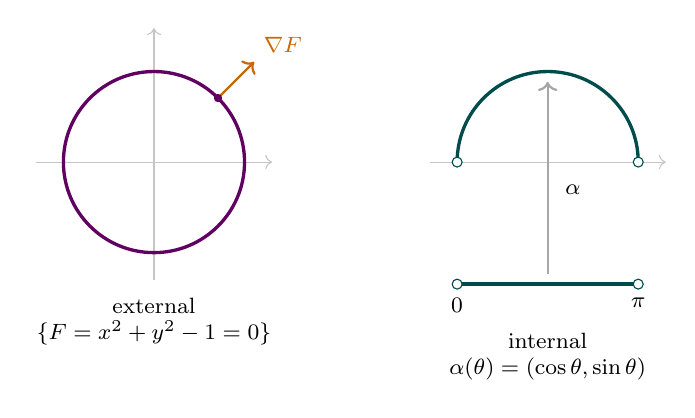
\begin{tikzpicture}[scale=1.0]
\draw[gray!45,->] (-1.5,0)--(1.5,0); \draw[gray!45,->] (0,-1.5)--(0,1.7);
\draw[violet!75!black,very thick] (0,0) circle (1.15);
\draw[orange!80!black,->,thick] (45:1.15) -- (45:1.8);
\node[orange!80!black,font=\footnotesize,anchor=south west] at (45:1.8) {$\nabla F$};
\fill[violet!75!black] (45:1.15) circle (1.5pt);
\node[font=\footnotesize,anchor=north,align=center] at (0,-1.6) {external\\ $\{F=x^2+y^2-1=0\}$};
\begin{scope}[xshift=5.0cm]
\draw[gray!45,->] (-1.5,0)--(1.5,0);
\draw[teal!60!black,very thick] (0:1.15) arc (0:180:1.15);
\draw[teal!60!black, fill=white] (1.15,0) circle (1.8pt); \draw[teal!60!black, fill=white] (-1.15,0) circle (1.8pt);
\draw[teal!60!black,very thick] (-1.15,-1.55) -- (1.15,-1.55);
\draw[teal!60!black, fill=white] (-1.15,-1.55) circle (1.8pt); \draw[teal!60!black, fill=white] (1.15,-1.55) circle (1.8pt);
\node[font=\footnotesize,below] at (-1.15,-1.6) {$0$};
\node[font=\footnotesize,below] at (1.15,-1.6) {$\pi$};
\draw[->,thick,gray!70] (0,-1.42) -- (0,1.02);
\node[font=\footnotesize,anchor=west] at (0.1,-0.35) {$\alpha$};
\node[font=\footnotesize,anchor=north,align=center] at (0,-2.05) {internal\\ $\alpha(\theta)=(\cos\theta,\sin\theta)$};
\end{scope}
\end{tikzpicture}
\end{center}


\begin{rembox}[A Parametrization Is an Inverse Chart]\label{rem:parametrization-inverse-chart}
``A parametrization is just another name for my inverse'' --- if $(U, \varphi)$ is a chart then $\varphi^{-1} : \varphi(U) \to U$ is a parametrization, and conversely. The internal description is therefore the chart picture of Chapter 1 with the extra demand that the map be smooth with injective differential; the external one is the level-set picture of \S\ref{sub:classical-manifolds}. Theorem~\ref{thm:ext-int} says the two carry the same information locally, which is why one may pass freely between ``solve the equations'' and ``draw the parametrization'' --- ``the same thing.''
\end{rembox}


% ============================================================================
% Lecture 6 (Mon Sep 14, 2026)
% SECTION 7.7: SMOOTH STRUCTURES ON REGULAR LEVEL SETS
% ============================================================================
\subsection{Smooth Structures on Regular Level Sets}\label{sub:level-smooth}

\textit{Lecture 6. Theorem~\ref{thm:regular-value} produced a \emph{topological} manifold from a regular level set. The charts it produced were not arbitrary, and the point of this subsection is that they are automatically smoothly compatible --- so the regular value theorem is in fact a machine for manufacturing smooth manifolds. ``This is a powerful way of constructing examples.''}

Recall the construction in the proof of Theorem~\ref{thm:regular-value}. Index the coordinates of $\mathbb{R}^{n+k}$ by $\{1, \ldots, n+k\}$. For $p \in M = F^{-1}(c)$, the hypothesis $\operatorname{rank} F'(p) = k$ says that some $k$ of the $n+k$ columns of $F'(p)$ are linearly independent. Choose such a set of indices $J$, $|J| = k$, and let $I = \{1,\ldots,n+k\} \setminus J$ be the complementary $n$ indices. Write $x_J \in \mathbb{R}^J$ and $x_I \in \mathbb{R}^I$ for the corresponding groups of coordinates. The implicit function theorem then solves for $x_J$ in terms of $x_I$: there are an open box $U_J \times V_J' \ni p$ and a smooth $h_J : V_J \to \mathbb{R}^J$ with
\[
F(x) = c \iff x_J = h_J(x_I) \qquad \text{for } x \text{ in the box},
\]
and the chart is the restriction to $M$ of the linear projection $\pi_I : \mathbb{R}^{n+k} \to \mathbb{R}^I$,
\[
\begin{aligned}
\varphi_J &: U_J \to V_J \subseteq \mathbb{R}^I, &\quad \varphi_J &= \pi_I|_{U_J}, \\
\varphi_J^{-1} &: V_J \to \mathbb{R}^{n+k}, &\quad \varphi_J^{-1}(u) &= \text{the point with } x_I = u,\ x_J = h_J(u).
\end{aligned}
\]
The inverse $\varphi_J^{-1}$ is a parametrization of that piece of $M$, in the following sense.

\begin{defbox}[Parametrization]\deflabel{def:parametrization}
Let $(U, \varphi)$ be a chart of a manifold $M$. The inverse $\varphi^{-1} : \varphi(U) \to U$ is the \textbf{parametrization} of $U$ determined by the chart. When $M \subseteq \mathbb{R}^N$, it is also regarded as a map $\varphi(U) \to \mathbb{R}^N$.
\leeref{Ch.~1, \emph{Coordinate Charts} (``local parametrization)}
\end{defbox}

\begin{propbox}[Regular Level Sets Are Smooth Manifolds]\thmlabel{prop:level-set-smooth}
Let $W \subseteq \mathbb{R}^{n+k}$ be open, $F : W \to \mathbb{R}^k$ smooth, and $c \in \mathbb{R}^k$ a regular value. Then the charts $\{(U_J, \varphi_J)\}$ above form a $C^\infty$ atlas on $M = F^{-1}(c)$, and $M$ is a smooth manifold of dimension $n$.
\leeref{Example 1.32 and Corollary 5.14}
\end{propbox}

\begin{center}
\begin{tikzcd}[row sep=3em, column sep=1.6em]
& \mathbb{R}^{n+k} \arrow[dr, "\pi_{I'}"] & \\
\varphi_J(U_J \cap U_{J'}) \arrow[ur, "\varphi_J^{-1}"] \arrow[rr, "\varphi_{J'} \circ \varphi_J^{-1}"'] & & \varphi_{J'}(U_J \cap U_{J'})
\end{tikzcd}
\end{center}

The proof in one picture. The transition function between two graph charts factors through the ambient space: a parametrization up, followed by a linear projection down. Both legs are smooth in the Euclidean sense, so the composite is.



\begin{proof}
\textit{(Lecture 6 worked the surface of Example~\ref{ex:surface-transition} first, then gave this general argument: ``the general thing is just harder to write.'')} The domains cover $M$, since each $p \in M$ lies in some $U_J$. Let $(U_J, \varphi_J)$ and $(U_{J'}, \varphi_{J'})$ be two of the charts, with complementary index sets $I$ and $I'$. Two observations, each valid for every choice of $J$:
\begin{enumerate}
    \item $\varphi_J^{-1} : V_J \to \mathbb{R}^{n+k}$ is smooth \emph{in the Euclidean sense}: its components are either coordinates of $u$ or components of the smooth map $h_J$.
    \item $\varphi_{J'}$ is the restriction of the linear map $\pi_{I'}$, which is smooth on all of $\mathbb{R}^{n+k}$.
\end{enumerate}
The transition function is the composite of the two. On the open set $\varphi_J(U_J \cap U_{J'}) \subseteq \mathbb{R}^I$,
\[
\varphi_{J'} \circ \varphi_J^{-1} = \pi_{I'} \circ \varphi_J^{-1},
\]
a composite of smooth maps between open subsets of Euclidean spaces, hence smooth. Exchanging the roles of $J$ and $J'$ shows $\varphi_J \circ \varphi_{J'}^{-1}$ is smooth as well, so the transition function is a diffeomorphism and the two charts are $C^\infty$-compatible (Definition~\ref{def:compatible}). By Theorem~\ref{thm:maximal-atlas} the atlas determines a smooth structure, of dimension $n$ by Theorem~\ref{thm:regular-value}.
\end{proof}
\begin{exbox}[A Surface in $\mathbb{R}^3$]\exlabel{ex:surface-transition}
The case $n = 2$, $k = 1$, where the indices can be written out. Let $F : W \subseteq \mathbb{R}^3 \to \mathbb{R}$ be smooth with regular value $c$, so $M = F^{-1}(c)$ is a surface and $F'(p) = \nabla F(p) \neq 0$ for $p \in M$. Suppose that at $p$ \emph{two} partial derivatives are nonzero, say $\partial F/\partial z(p) \neq 0$ and $\partial F/\partial y(p) \neq 0$. Then $p$ lies in the domains of two charts built from different solved-for variables:
\[
\begin{aligned}
\text{solving for } z: &\quad z = g(x,y), &\quad \varphi : U \to \mathbb{R}^2, &\quad \varphi(x,y,z) = (x,y);\\
\text{solving for } y: &\quad y = h(x,z), &\quad \psi : V \to \mathbb{R}^2, &\quad \psi(x,y,z) = (x,z).
\end{aligned}
\]
The parametrization inverse to $\varphi$ is $\varphi^{-1}(x,y) = (x,\,y,\,g(x,y))$, and composing with $\psi$ --- which reads off the first and third coordinates --- gives the transition function
\[
\psi \circ \varphi^{-1}(x,y) = \big(x,\; g(x,y)\big),
\]
smooth because $g$ is. In the other direction $\varphi \circ \psi^{-1}(x,z) = \big(x,\, h(x,z)\big)$, smooth because $h$ is. So $(U,\varphi)$ and $(V,\psi)$ are compatible, and the same picture is what Proposition~\ref{prop:level-set-smooth} formalizes: the overlap of two charts is the part of the surface expressible as a graph over two different pairs of variables, and the transition function converts one graph into the other.
\end{exbox}

The same level sets are submanifolds in the sense of Lecture~12, and their graph-chart structure is the induced one (Proposition~\ref{prop:rvt-agree}).

\begin{rembox}\label{rem:euclidean}
The only thing that varies between charts is \emph{which} $k$ coordinates are solved for, and the whole proof is the observation that a projection composed with a parametrization is smooth no matter which choice is made. Uribe made the same point while declining to write the general indices out: ``the notation becomes a mess, but it's the same thing.'' Note also that the charts are graphs of smooth maps, which is what makes the parametrization smooth --- the topological argument of Theorem~\ref{thm:regular-value} only needed $h_J$ continuous.
\end{rembox}

\begin{center}
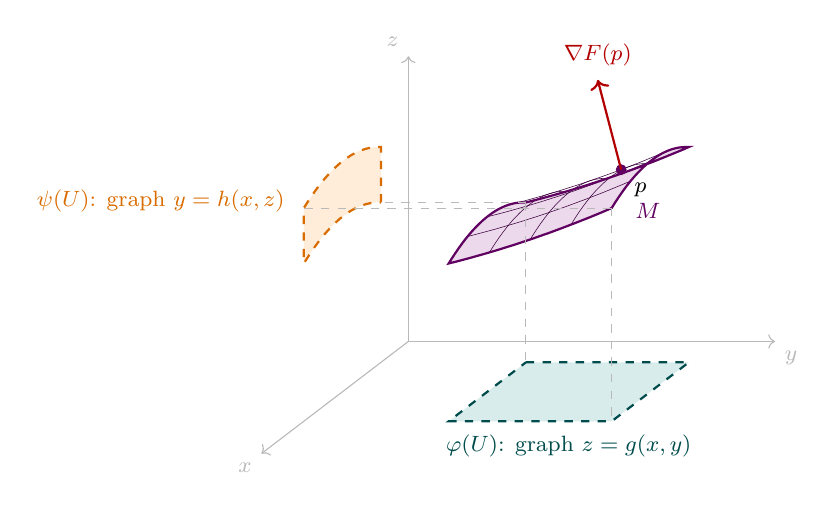
\begin{tikzpicture}[scale=1.15]
\fill[violet!15] (1.298,1.535) -- (1.376,1.555) -- (1.454,1.575) -- (1.532,1.596) -- (1.611,1.618) -- (1.689,1.640) -- (1.767,1.663) -- (1.845,1.687) -- (1.924,1.711) -- (2.002,1.736) -- (2.080,1.761) -- (2.158,1.787) -- (2.237,1.814) -- (2.315,1.841) -- (2.393,1.869) -- (2.471,1.897) -- (2.550,1.926) -- (2.628,1.956) -- (2.706,1.986) -- (2.784,2.017) -- (2.863,2.049) -- (2.941,2.081) -- (3.019,2.113) -- (3.097,2.147) -- (3.097,2.147) -- (3.060,2.147) -- (3.023,2.145) -- (2.986,2.141) -- (2.949,2.133) -- (2.912,2.123) -- (2.875,2.110) -- (2.838,2.094) -- (2.801,2.076) -- (2.764,2.055) -- (2.727,2.031) -- (2.690,2.004) -- (2.653,1.975) -- (2.616,1.943) -- (2.579,1.908) -- (2.542,1.871) -- (2.504,1.830) -- (2.467,1.787) -- (2.430,1.742) -- (2.393,1.693) -- (2.356,1.642) -- (2.319,1.588) -- (2.282,1.532) -- (2.245,1.473) -- (2.245,1.473) -- (2.167,1.439) -- (2.088,1.406) -- (2.010,1.374) -- (1.932,1.343) -- (1.854,1.312) -- (1.775,1.282) -- (1.697,1.252) -- (1.619,1.223) -- (1.541,1.194) -- (1.462,1.167) -- (1.384,1.139) -- (1.306,1.113) -- (1.228,1.087) -- (1.149,1.061) -- (1.071,1.037) -- (0.993,1.012) -- (0.915,0.989) -- (0.836,0.966) -- (0.758,0.944) -- (0.680,0.922) -- (0.602,0.901) -- (0.523,0.880) -- (0.445,0.861) -- (0.445,0.861) -- (0.482,0.920) -- (0.519,0.976) -- (0.556,1.030) -- (0.593,1.081) -- (0.630,1.130) -- (0.667,1.175) -- (0.704,1.218) -- (0.742,1.259) -- (0.779,1.296) -- (0.816,1.331) -- (0.853,1.363) -- (0.890,1.392) -- (0.927,1.419) -- (0.964,1.443) -- (1.001,1.464) -- (1.038,1.482) -- (1.075,1.498) -- (1.112,1.511) -- (1.149,1.521) -- (1.186,1.529) -- (1.223,1.533) -- (1.260,1.535) -- (1.298,1.535) -- cycle;
\draw[violet!45!black,very thin] (1.747,1.657) -- (1.710,1.658) -- (1.673,1.656) -- (1.636,1.651) -- (1.599,1.644) -- (1.562,1.633) -- (1.525,1.620) -- (1.488,1.605) -- (1.451,1.586) -- (1.414,1.565) -- (1.377,1.541) -- (1.340,1.515) -- (1.303,1.485) -- (1.266,1.453) -- (1.229,1.419) -- (1.192,1.381) -- (1.154,1.341) -- (1.117,1.298) -- (1.080,1.252) -- (1.043,1.204) -- (1.006,1.153) -- (0.969,1.099) -- (0.932,1.042) -- (0.895,0.983);
\draw[violet!45!black,very thin] (2.197,1.800) -- (2.160,1.801) -- (2.123,1.799) -- (2.086,1.794) -- (2.049,1.787) -- (2.012,1.776) -- (1.975,1.763) -- (1.938,1.748) -- (1.901,1.729) -- (1.864,1.708) -- (1.827,1.684) -- (1.790,1.658) -- (1.753,1.628) -- (1.716,1.596) -- (1.679,1.562) -- (1.642,1.524) -- (1.604,1.484) -- (1.567,1.441) -- (1.530,1.395) -- (1.493,1.347) -- (1.456,1.296) -- (1.419,1.242) -- (1.382,1.185) -- (1.345,1.126);
\draw[violet!45!black,very thin] (2.647,1.963) -- (2.610,1.964) -- (2.573,1.962) -- (2.536,1.957) -- (2.499,1.950) -- (2.462,1.939) -- (2.425,1.926) -- (2.388,1.911) -- (2.351,1.892) -- (2.314,1.871) -- (2.277,1.847) -- (2.240,1.821) -- (2.203,1.791) -- (2.166,1.759) -- (2.129,1.725) -- (2.092,1.687) -- (2.054,1.647) -- (2.017,1.604) -- (1.980,1.558) -- (1.943,1.510) -- (1.906,1.459) -- (1.869,1.405) -- (1.832,1.348) -- (1.795,1.289);
\draw[violet!45!black,very thin] (1.083,1.501) -- (1.161,1.521) -- (1.240,1.541) -- (1.318,1.562) -- (1.396,1.584) -- (1.474,1.606) -- (1.553,1.629) -- (1.631,1.653) -- (1.709,1.677) -- (1.787,1.702) -- (1.866,1.727) -- (1.944,1.753) -- (2.022,1.780) -- (2.100,1.807) -- (2.179,1.835) -- (2.257,1.863) -- (2.335,1.892) -- (2.413,1.922) -- (2.492,1.952) -- (2.570,1.983) -- (2.648,2.015) -- (2.726,2.047) -- (2.805,2.079) -- (2.883,2.113);
\draw[violet!45!black,very thin] (0.868,1.376) -- (0.947,1.396) -- (1.025,1.416) -- (1.103,1.437) -- (1.182,1.459) -- (1.260,1.481) -- (1.338,1.504) -- (1.416,1.528) -- (1.495,1.552) -- (1.573,1.577) -- (1.651,1.602) -- (1.729,1.628) -- (1.808,1.655) -- (1.886,1.682) -- (1.964,1.710) -- (2.042,1.738) -- (2.121,1.767) -- (2.199,1.797) -- (2.277,1.827) -- (2.355,1.858) -- (2.434,1.889) -- (2.512,1.922) -- (2.590,1.954) -- (2.668,1.988);
\draw[violet!45!black,very thin] (0.654,1.159) -- (0.732,1.179) -- (0.811,1.200) -- (0.889,1.221) -- (0.967,1.242) -- (1.045,1.265) -- (1.124,1.288) -- (1.202,1.311) -- (1.280,1.335) -- (1.358,1.360) -- (1.437,1.385) -- (1.515,1.411) -- (1.593,1.438) -- (1.671,1.465) -- (1.750,1.493) -- (1.828,1.522) -- (1.906,1.551) -- (1.984,1.580) -- (2.063,1.611) -- (2.141,1.641) -- (2.219,1.673) -- (2.297,1.705) -- (2.376,1.738) -- (2.454,1.771);
\draw[violet!75!black,thick] (1.298,1.535) -- (1.376,1.555) -- (1.454,1.575) -- (1.532,1.596) -- (1.611,1.618) -- (1.689,1.640) -- (1.767,1.663) -- (1.845,1.687) -- (1.924,1.711) -- (2.002,1.736) -- (2.080,1.761) -- (2.158,1.787) -- (2.237,1.814) -- (2.315,1.841) -- (2.393,1.869) -- (2.471,1.897) -- (2.550,1.926) -- (2.628,1.956) -- (2.706,1.986) -- (2.784,2.017) -- (2.863,2.049) -- (2.941,2.081) -- (3.019,2.113) -- (3.097,2.147) -- (3.097,2.147) -- (3.060,2.147) -- (3.023,2.145) -- (2.986,2.141) -- (2.949,2.133) -- (2.912,2.123) -- (2.875,2.110) -- (2.838,2.094) -- (2.801,2.076) -- (2.764,2.055) -- (2.727,2.031) -- (2.690,2.004) -- (2.653,1.975) -- (2.616,1.943) -- (2.579,1.908) -- (2.542,1.871) -- (2.504,1.830) -- (2.467,1.787) -- (2.430,1.742) -- (2.393,1.693) -- (2.356,1.642) -- (2.319,1.588) -- (2.282,1.532) -- (2.245,1.473) -- (2.245,1.473) -- (2.167,1.439) -- (2.088,1.406) -- (2.010,1.374) -- (1.932,1.343) -- (1.854,1.312) -- (1.775,1.282) -- (1.697,1.252) -- (1.619,1.223) -- (1.541,1.194) -- (1.462,1.167) -- (1.384,1.139) -- (1.306,1.113) -- (1.228,1.087) -- (1.149,1.061) -- (1.071,1.037) -- (0.993,1.012) -- (0.915,0.989) -- (0.836,0.966) -- (0.758,0.944) -- (0.680,0.922) -- (0.602,0.901) -- (0.523,0.880) -- (0.445,0.861) -- (0.445,0.861) -- (0.482,0.920) -- (0.519,0.976) -- (0.556,1.030) -- (0.593,1.081) -- (0.630,1.130) -- (0.667,1.175) -- (0.704,1.218) -- (0.742,1.259) -- (0.779,1.296) -- (0.816,1.331) -- (0.853,1.363) -- (0.890,1.392) -- (0.927,1.419) -- (0.964,1.443) -- (1.001,1.464) -- (1.038,1.482) -- (1.075,1.498) -- (1.112,1.511) -- (1.149,1.521) -- (1.186,1.529) -- (1.223,1.533) -- (1.260,1.535) -- (1.298,1.535) -- cycle;
\fill[teal!15] (1.298,-0.231) -- (1.898,-0.231) -- (2.497,-0.231) -- (3.097,-0.231) -- (3.097,-0.231) -- (2.813,-0.448) -- (2.529,-0.665) -- (2.245,-0.882) -- (2.245,-0.882) -- (1.645,-0.882) -- (1.045,-0.882) -- (0.445,-0.882) -- (0.445,-0.882) -- (0.729,-0.665) -- (1.013,-0.448) -- (1.298,-0.231) -- cycle;  \draw[teal!60!black,thick,dashed] (1.298,-0.231) -- (1.898,-0.231) -- (2.497,-0.231) -- (3.097,-0.231) -- (3.097,-0.231) -- (2.813,-0.448) -- (2.529,-0.665) -- (2.245,-0.882) -- (2.245,-0.882) -- (1.645,-0.882) -- (1.045,-0.882) -- (0.445,-0.882) -- (0.445,-0.882) -- (0.729,-0.665) -- (1.013,-0.448) -- (1.298,-0.231) -- cycle;
\fill[orange!15] (-0.303,1.535) -- (-0.303,1.565) -- (-0.303,1.598) -- (-0.303,1.631) -- (-0.303,1.666) -- (-0.303,1.703) -- (-0.303,1.741) -- (-0.303,1.780) -- (-0.303,1.821) -- (-0.303,1.863) -- (-0.303,1.907) -- (-0.303,1.952) -- (-0.303,1.998) -- (-0.303,2.046) -- (-0.303,2.096) -- (-0.303,2.147) -- (-0.303,2.147) -- (-0.359,2.147) -- (-0.416,2.140) -- (-0.473,2.127) -- (-0.530,2.108) -- (-0.587,2.082) -- (-0.643,2.050) -- (-0.700,2.011) -- (-0.757,1.967) -- (-0.814,1.915) -- (-0.871,1.857) -- (-0.928,1.793) -- (-0.985,1.723) -- (-1.041,1.646) -- (-1.098,1.562) -- (-1.155,1.473) -- (-1.155,1.473) -- (-1.155,1.422) -- (-1.155,1.372) -- (-1.155,1.324) -- (-1.155,1.278) -- (-1.155,1.232) -- (-1.155,1.189) -- (-1.155,1.147) -- (-1.155,1.106) -- (-1.155,1.066) -- (-1.155,1.029) -- (-1.155,0.992) -- (-1.155,0.957) -- (-1.155,0.923) -- (-1.155,0.891) -- (-1.155,0.861) -- (-1.155,0.861) -- (-1.098,0.950) -- (-1.041,1.034) -- (-0.985,1.111) -- (-0.928,1.181) -- (-0.871,1.245) -- (-0.814,1.303) -- (-0.757,1.355) -- (-0.700,1.399) -- (-0.644,1.438) -- (-0.587,1.470) -- (-0.530,1.496) -- (-0.473,1.515) -- (-0.416,1.528) -- (-0.359,1.535) -- (-0.303,1.535) -- cycle;  \draw[orange!85!black,thick,dashed] (-0.303,1.535) -- (-0.303,1.565) -- (-0.303,1.598) -- (-0.303,1.631) -- (-0.303,1.666) -- (-0.303,1.703) -- (-0.303,1.741) -- (-0.303,1.780) -- (-0.303,1.821) -- (-0.303,1.863) -- (-0.303,1.907) -- (-0.303,1.952) -- (-0.303,1.998) -- (-0.303,2.046) -- (-0.303,2.096) -- (-0.303,2.147) -- (-0.303,2.147) -- (-0.359,2.147) -- (-0.416,2.140) -- (-0.473,2.127) -- (-0.530,2.108) -- (-0.587,2.082) -- (-0.643,2.050) -- (-0.700,2.011) -- (-0.757,1.967) -- (-0.814,1.915) -- (-0.871,1.857) -- (-0.928,1.793) -- (-0.985,1.723) -- (-1.041,1.646) -- (-1.098,1.562) -- (-1.155,1.473) -- (-1.155,1.473) -- (-1.155,1.422) -- (-1.155,1.372) -- (-1.155,1.324) -- (-1.155,1.278) -- (-1.155,1.232) -- (-1.155,1.189) -- (-1.155,1.147) -- (-1.155,1.106) -- (-1.155,1.066) -- (-1.155,1.029) -- (-1.155,0.992) -- (-1.155,0.957) -- (-1.155,0.923) -- (-1.155,0.891) -- (-1.155,0.861) -- (-1.155,0.861) -- (-1.098,0.950) -- (-1.041,1.034) -- (-0.985,1.111) -- (-0.928,1.181) -- (-0.871,1.245) -- (-0.814,1.303) -- (-0.757,1.355) -- (-0.700,1.399) -- (-0.644,1.438) -- (-0.587,1.470) -- (-0.530,1.496) -- (-0.473,1.515) -- (-0.416,1.528) -- (-0.359,1.535) -- (-0.303,1.535) -- cycle;
\draw[gray!55,dashed] (1.298,1.535) -- (1.298,-0.231);
\draw[gray!55,dashed] (1.298,1.535) -- (-0.303,1.535);
\draw[gray!55,dashed] (2.245,1.473) -- (2.245,-0.882);
\draw[gray!55,dashed] (2.245,1.473) -- (-1.155,1.473);
\fill[violet!75!black] (2.350,1.897) circle (1.7pt);
\draw[red!70!black,->,thick] (2.350,1.897) -- (2.091,2.889);
\node[font=\footnotesize,anchor=north west] at (2.390,1.857) {$p$};
\node[red!70!black,font=\footnotesize,anchor=south] at (2.091,2.929) {$\nabla F(p)$};
\node[violet!75!black,font=\footnotesize,anchor=west] at (2.40,1.44) {$M$};
\node[teal!60!black,font=\footnotesize,anchor=north] at (1.771,-0.92) {$\varphi(U)$: graph $z=g(x,y)$};
\node[orange!85!black,font=\footnotesize,anchor=east] at (-1.26,1.55) {$\psi(U)$: graph $y=h(x,z)$};
\draw[gray!55,->] (0,0) -- (-1.623,-1.239) node[anchor=north east,font=\footnotesize]{$x$};
\draw[gray!55,->] (0,0) -- (4.050,0.000) node[anchor=north west,font=\footnotesize]{$y$};
\draw[gray!55,->] (0,0) -- (0.000,3.150) node[anchor=south east,font=\footnotesize]{$z$};
\end{tikzpicture}
\end{center}

The board picture for this example. The patch $M$ is drawn over a rectangle of $(x,y)$, and the two shaded regions are its images under the two charts: straight down onto the $xy$-plane, giving $\varphi(U)$ and presenting $M$ as $z = g(x,y)$; and sideways onto the $xz$-plane, giving $\psi(U)$ and presenting the \emph{same} patch as $y = h(x,z)$. The transition function is the trip up from one shadow and down to the other.

The picture only works because $\partial F/\partial z$ and $\partial F/\partial y$ are \emph{both} nonzero throughout the patch. If $\partial F/\partial y$ vanished anywhere --- if the surface were vertical in the $y$-direction there --- the sideways projection would fold over and $\psi$ would not be injective, so there would be no second chart and nothing to compare. Which pairs of variables work is a condition at each point, and in general it changes from point to point; that is the content of the index set $J$ in Proposition~\ref{prop:level-set-smooth}.

\textbf{Transcription note.} The board wrote the parametrization as ``$\psi^{-1}(x,y) = (x,y,g(x,y))$''; it is $\varphi^{-1}$, as the recording confirms. The board also wrote ``$\varphi^{-1}|_{U \cap V} : U \cap V \to \mathbb{R}^{n+k}$'' --- but $\varphi^{-1}$ is defined on $\varphi(U \cap V) \subseteq \mathbb{R}^n$, not on $U \cap V$, which consists of points of the manifold. Two further slips in the statement of the regular value theorem: the value $c$ lies in $\mathbb{R}^k$, not $\mathbb{R}^{n+k}$; and the rank condition is on the Jacobian $F'(p)$, not on $F^{-1}(p)$.

\begin{lembox}[Smooth Maps into and out of Regular Level Sets]\thmlabel{lem:level-set-maps}
Let $M = F^{-1}(c)$ be a regular level set in $\mathbb{R}^{n+k}$, with the smooth structure of Proposition~\ref{prop:level-set-smooth}.
\begin{enumerate}
    \item If $W' \subseteq \mathbb{R}^{n+k}$ is open and $H : W' \to \mathbb{R}^l$ is smooth, then the restriction $H|_{M \cap W'} : M \cap W' \to \mathbb{R}^l$ is smooth.
    \item If $P$ is a smooth manifold and $G : P \to \mathbb{R}^{n+k}$ is smooth with $G(P) \subseteq M$, then $G$ is smooth as a map $P \to M$.
\end{enumerate}
\leeref{cf.\ Ch.~5, \emph{Restricting Maps to Submanifolds}}
\end{lembox}

\begin{proof}
(1) $M \cap W'$ is open in $M$. For a graph chart $(U_J, \varphi_J)$, the parametrization $\varphi_J^{-1}$ is smooth into $\mathbb{R}^{n+k}$, so the coordinate representation $H \circ \varphi_J^{-1}$ is a composite of smooth maps between open subsets of Euclidean spaces. (2) $G$ is continuous into $M$ for the subspace topology. Given $q \in P$, take a graph chart $(U_J, \varphi_J)$ of $M$ at $G(q)$ and a chart $(V, \chi)$ of $P$ at $q$ with $G(V) \subseteq U_J$ (shrink $V$ to $V \cap G^{-1}(U_J)$). Then $\varphi_J \circ G \circ \chi^{-1} = \pi_I \circ (G \circ \chi^{-1})$ is a linear projection of a smooth map, hence smooth.
\end{proof}

Not stated in lecture; filled in because it is used repeatedly --- tacitly in the next proof, and explicitly for $S^n \to \mathbb{RP}^n$ in \ref{sec:special-maps}. In words: maps \emph{out of} a level set may be computed by restricting ambient formulas, and maps \emph{into} one may be computed as maps into the ambient space.

\begin{propbox}[The Three Circle Atlases Define One Smooth Structure]\thmlabel{prop:circle-atlases-same}
The four-chart atlas (Example~\ref{ex:circle-four}), the angle atlas (Example~\ref{ex:circle-angle}) and the stereographic atlas (Example~\ref{ex:circle-stereo}) on $S^1$ are pairwise compatible. All three generate the smooth structure that Proposition~\ref{prop:level-set-smooth} gives $S^1 = F^{-1}(1)$, $F(x,y) = x^2 + y^2$.
\end{propbox}

\begin{proof}
For $S^1$ the graph charts of Proposition~\ref{prop:level-set-smooth} are the four projection charts, so that atlas $\mathcal{A}$ is the four-chart atlas. It suffices to show that every chart $(V, \chi)$ of the other two atlases is compatible with every chart $(U, \varphi)$ of $\mathcal{A}$. All such charts then lie in the maximal atlas $\overline{\mathcal{A}}$ (Theorem~\ref{thm:maximal-atlas}), and any two charts of an atlas are compatible --- which is how Proposition~\ref{prop:compat-not-transitive} is circumvented.

Each such $\chi$ has two properties.
\begin{itemize}
    \item[(a)] $\chi^{-1}$ is smooth as a map into $\mathbb{R}^2$: it is $\theta \mapsto (\cos\theta, \sin\theta)$ for the angle charts, $u \mapsto \big(2u,\, u^2 - 1\big)/(u^2+1)$ for $\sigma_N$, and similarly for $\sigma_S$.
    \item[(b)] $\chi$ is the restriction to $V$ of a smooth function $\hat\chi$ on an open subset of $\mathbb{R}^2$ containing $V$. For $\sigma_N = x/(1-y)$ take $\{y < 1\}$, and for $\sigma_S = x/(1+y)$ take $\{y > -1\}$. For an angle chart take a smooth branch of the argument on the plane minus a closed ray: for values in $(-\pi, \pi)$, $\theta = 2\arctan\big(y/(x + \sqrt{x^2+y^2})\big)$, and other ranges follow by rotating and adding a constant.
\end{itemize}
On the overlap, $\varphi \circ \chi^{-1} = \pi \circ \chi^{-1}$ with $\pi$ a linear projection, which is smooth by (a). And $\chi \circ \varphi^{-1} = \hat\chi \circ \varphi^{-1}$ is smooth by (b), $\varphi^{-1}$ being a smooth parametrization.
\end{proof}

\section{Linear Algebra Toolkit}\label{sec:vector-spaces}

\roadmark{Stage: linear}{The tool both tangent spaces will need: the linear algebra used from here on. The differential of a map between vector spaces (\ref{sec:vs-differential}) and the smooth matrix groups (\ref{sec:on-un-smooth}) follow.}

\label{sub:linalg-toolkit}

\textit{Not from lecture. From here on the course runs on linear algebra --- differentials, bases of tangent spaces, dual spaces --- and this section records, once, the facts used. The first box is imported from linear algebra without proof, as the point-set facts of \ref{sec:review} were imported from 590; everything after it is proved.} Throughout, vector spaces are real.

\begin{propbox}[Standing Facts from Linear Algebra]\thmlabel{fact:linalg}
Let $A : V \to W$ be linear, with $V$ and $W$ finite-dimensional.
\begin{enumerate}
    \item \emph{Rank--nullity.} $\dim V = \dim\ker A + \operatorname{rank} A$. Consequently: if $A$ is injective then $\dim V \le \dim W$; if $A$ is surjective then $\dim V \ge \dim W$; and if $\dim V = \dim W$, then $A$ is injective $\iff$ surjective $\iff$ bijective.
    \item \emph{Bases determine linear maps.} A linear map is determined by its values on a basis, and any assignment of values to the vectors of a basis extends uniquely to a linear map. In particular, two linear maps that agree on a basis are equal.
    \item \emph{Matrices.} Given bases $(e_1, \ldots, e_m)$ of $V$ and $(f_1, \ldots, f_n)$ of $W$, the matrix $[A] = (a_{ij})$ of $A$ is defined by $A e_j = \sum_i a_{ij} f_i$: its $j$-th \emph{column} holds the coordinates of $Ae_j$. Composition corresponds to matrix multiplication, $[AB] = [A][B]$, and $\operatorname{rank} A$ is the rank of $[A]$, which equals the rank of its transpose.
    \item \emph{Change of basis.} If $e'_j = \sum_i P_{ij}\, e_i$ and $f'_l = \sum_k Q_{kl}\, f_k$ are new bases, with $P$ and $Q$ invertible, then the matrix of $A$ in the new bases is $Q^{-1} [A] P$.
\end{enumerate}
\leeref{Corollary B.21 and Proposition B.24}
\end{propbox}

\begin{proof}[Proof (to be filled)]
Imported from linear algebra without proof; proved in Axler, \emph{Linear Algebra Done Right} (see also Lee, Corollary~B.21 and Proposition~B.24). To be filled.
\end{proof}

\begin{defbox}[Dual Space]\deflabel{def:dual}
The \textbf{dual space} of $V$ is $V^* = \{\lambda : V \to \mathbb{R} \mid \lambda \text{ linear}\}$, a vector space under pointwise operations; its elements are \textbf{linear functionals}, or \textbf{covectors}.
\leeref{Proposition 11.1}
\end{defbox}

\begin{defbox}[Dual Basis]\deflabel{def:dual-basis}
If $(e_1, \ldots, e_n)$ is a basis of $V$, the \textbf{dual basis} $(\varepsilon^1, \ldots, \varepsilon^n)$ consists of the covectors (Definition~\ref{def:dual}) with
\[
\varepsilon^i(e_j) = \delta^i_j ,
\]
which exist and are unique by Proposition~\ref{fact:linalg}(2).
\leeref{Proposition 11.1}
\end{defbox}

\begin{propbox}[The Dual Basis]\thmlabel{prop:dual-basis}
Let $(e_1, \ldots, e_n)$ be a basis of $V$ with dual basis $(\varepsilon^1, \ldots, \varepsilon^n)$. Then $(\varepsilon^i)$ is a basis of $V^*$, so $\dim V^* = \dim V$, and for all $v \in V$ and $\lambda \in V^*$,
\[
v = \sum_{i=1}^n \varepsilon^i(v)\, e_i, \qquad\qquad \lambda = \sum_{i=1}^n \lambda(e_i)\, \varepsilon^i .
\]
\leeref{Proposition 11.1}
\end{propbox}

\begin{proof}
If $v = \sum_j v^j e_j$, then $\varepsilon^i(v) = \sum_j v^j \delta^i_j = v^i$, which is the first formula: the dual basis \emph{extracts the components} of a vector. The two sides of the second formula are covectors that agree on each $e_j$, both giving $\lambda(e_j)$, so they are equal by Proposition~\ref{fact:linalg}(2); hence the $\varepsilon^i$ span $V^*$. If $\sum_i c_i \varepsilon^i = 0$, applying it to $e_j$ gives $c_j = 0$; so they are independent.
\end{proof}

\begin{propbox}[The Double Dual]\thmlabel{prop:double-dual}
For a finite-dimensional $V$, the map
\[
\iota : V \to V^{**}, \qquad \iota(v)(\lambda) = \lambda(v),
\]
is a linear isomorphism. It is \textbf{canonical}: its definition involves no choice of basis.
\leeref{Proposition 11.8}
\end{propbox}

\begin{proof}
$\iota$ is linear, since each $\lambda$ is. If $v \ne 0$, extend $v$ to a basis $(v, e_2, \ldots, e_n)$; the first dual basis covector $\varepsilon^1$ has $\iota(v)(\varepsilon^1) = \varepsilon^1(v) = 1 \ne 0$. So $\iota$ is injective, and $\dim V^{**} = \dim V^* = \dim V$ by Proposition~\ref{prop:dual-basis}, so $\iota$ is an isomorphism by Proposition~\ref{fact:linalg}(1).
\end{proof}

\begin{rembox}\label{rem:vector-spaces}
A finite-dimensional $V$ is also isomorphic to $V^*$, for instance by $e_i \mapsto \varepsilon^i$, but that isomorphism depends on the basis: change the basis and it changes. $V$ and $V^{**}$ are identified \emph{canonically}. This is why tangent vectors and covectors must be kept apart, as Lecture 10 did with $T_pM$ and $T_p^*M$, while the dual of $T_p^*M$ may be silently identified with $T_pM$.
\end{rembox}

\begin{defbox}[Dual Map]\deflabel{def:dual-map}
The \textbf{dual map}, or \textbf{transpose}, of a linear map $A : V \to W$ is
\[
A^* : W^* \to V^*, \qquad A^*(\lambda) = \lambda \circ A .
\]
\leeref{Proposition 11.4}
\end{defbox}

\begin{center}
\begin{tikzcd}[row sep=1.2em, column sep=4em]
V \arrow[r, "A"] & W & \text{vectors: forward} \\
V^* & W^* \arrow[l, "A^*"'] & \text{covectors: backward}
\end{tikzcd}
\end{center}

A covector on $W$ becomes a covector on $V$ by first applying $A$; so the dual map runs backwards. This is the linear-algebra shadow of the directions in \S\ref{sub:pushforward}, where germs were pulled back and derivations pushed forward.

\begin{propbox}[Properties of the Dual Map]\thmlabel{prop:dual-map}
Let $A : V \to W$ and $B : W \to Z$ be linear.
\begin{enumerate}
    \item $A^*$ is linear, $(\mathrm{id}_V)^* = \mathrm{id}_{V^*}$, and $(B \circ A)^* = A^* \circ B^*$. In particular, if $A$ is an isomorphism, so is $A^*$, with $(A^*)^{-1} = (A^{-1})^*$.
    \item For finite-dimensional $V$ and $W$, the matrix of $A^*$ in the dual bases is the transpose of the matrix of $A$.
    \item For finite-dimensional $V$ and $W$: $A$ is injective $\iff$ $A^*$ is surjective, and $A$ is surjective $\iff$ $A^*$ is injective.
\end{enumerate}
\leeref{Proposition 11.4}
\end{propbox}

\begin{proof}
(1) $A^*(\lambda + c\mu) = (\lambda + c\mu) \circ A = A^*\lambda + c\,A^*\mu$, and $(B \circ A)^*(\lambda) = \lambda \circ B \circ A = A^*(B^*\lambda)$. For an isomorphism, apply this to $A^{-1} \circ A = \mathrm{id}$ and $A \circ A^{-1} = \mathrm{id}$.

(2) Let $(e_j)$ and $(f_i)$ be bases of $V$ and $W$, with dual bases $(\varepsilon^j)$ and $(\varphi^k)$, and $Ae_j = \sum_i a_{ij} f_i$. Then $A^*(\varphi^k)(e_j) = \varphi^k(Ae_j) = a_{kj}$, so by Proposition~\ref{prop:dual-basis}, $A^*(\varphi^k) = \sum_j a_{kj}\,\varepsilon^j$. The $k$-th column of the matrix of $A^*$ is therefore the $k$-th row of $[A]$.

(3) By (2) and Proposition~\ref{fact:linalg}(3), $\operatorname{rank} A^* = \operatorname{rank} A$. Now $A$ is surjective iff $\operatorname{rank} A = \dim W$, iff $\operatorname{rank} A^* = \dim W^*$, which by rank--nullity means $A^*$ is injective. Likewise $A$ is injective iff $\operatorname{rank} A = \dim V = \dim V^*$, iff $A^*$ is surjective.
\end{proof}

\begin{defbox}[Bilinear Pairing]\deflabel{def:pairing}
A \textbf{bilinear pairing} is a map $B : V \times W \to \mathbb{R}$ that is linear in each argument separately. It induces linear maps
\[
B^\flat : V \to W^*, \ \ v \mapsto B(v, \cdot\,), \qquad\qquad B^\sharp : W \to V^*, \ \ w \mapsto B(\cdot\,, w).
\]
$B$ is \textbf{left non-degenerate} if $B(v, w) = 0$ for all $w$ implies $v = 0$, i.e.\ $B^\flat$ is injective; \textbf{right non-degenerate} if $B(v, w) = 0$ for all $v$ implies $w = 0$, i.e.\ $B^\sharp$ is injective; and \textbf{non-degenerate} if both.
\end{defbox}

\begin{thmbox}[Non-Degenerate Pairings]\thmlabel{thm:pairing}
Let $B : V \times W \to \mathbb{R}$ be a non-degenerate bilinear pairing, and suppose $V$ or $W$ is finite-dimensional. Then both are finite-dimensional, $\dim V = \dim W$, and
\[
B^\flat : V \xrightarrow{\ \cong\ } W^*, \qquad\qquad B^\sharp : W \xrightarrow{\ \cong\ } V^*
\]
are isomorphisms.
\leeref{no counterpart}
\end{thmbox}

\begin{proof}
Suppose $V$ is finite-dimensional, of dimension $n$; the other case is symmetric. Right non-degeneracy makes $B^\sharp : W \to V^*$ injective, so $W$ is isomorphic to a subspace of the $n$-dimensional $V^*$: it is finite-dimensional with $\dim W \le n$. Left non-degeneracy makes $B^\flat : V \to W^*$ injective, so $n \le \dim W^* = \dim W$. Hence $\dim V = \dim W$, and $B^\flat$, $B^\sharp$ are injective maps between spaces of equal finite dimension, hence isomorphisms by Proposition~\ref{fact:linalg}(1).
\end{proof}

\begin{rembox}\label{rem:vector-spaces-2}
Each half of non-degeneracy gives one inequality of dimensions, and it is the \emph{pair} of inequalities that forces the isomorphisms; neither half suffices alone. The finiteness hypothesis cannot be dropped: for an infinite-dimensional $V$, the evaluation pairing $V \times V^* \to \mathbb{R}$, $(v, \lambda) \mapsto \lambda(v)$, is non-degenerate, but its map $B^\flat = \iota : V \to V^{**}$ is injective without being onto. Assignment~3, Problem~3 is exactly a pairing $T_pM \times I_p/I_p^2 \to \mathbb{R}$ to which this theorem applies.
\end{rembox}

\begin{defbox}[Quotient Vector Space]\deflabel{def:quotient-vs}
Let $W \subseteq V$ be a linear subspace. The \textbf{quotient space} $V/W$ is the set of cosets $v + W = \{v + w \mid w \in W\}$, with
\[
(v + W) + (v' + W) = (v + v') + W, \qquad c\,(v + W) = cv + W,
\]
and the \textbf{projection} is $\pi : V \to V/W$, $\pi(v) = v + W$. Two vectors have the same coset iff their difference lies in $W$.
\leeref{App.~B, \emph{Vector Spaces}}
\end{defbox}

\begin{propbox}[Quotient Spaces and Their Universal Property]\thmlabel{prop:quotient-vs}
\begin{enumerate}
    \item The operations are well defined, $V/W$ is a vector space, and $\pi$ is linear and surjective with $\ker \pi = W$.
    \item \emph{Universal property.} If $A : V \to Z$ is linear with $W \subseteq \ker A$, there is a unique linear $\bar A : V/W \to Z$ with $\bar A \circ \pi = A$, namely $\bar A(v + W) = A(v)$.
    \item If $V$ is finite-dimensional, $\dim V/W = \dim V - \dim W$.
\end{enumerate}
\leeref{App.~B, \emph{Vector Spaces}}
\end{propbox}

\begin{proof}
(1) If $v - v' \in W$ and $u - u' \in W$, then $(v + u) - (v' + u') \in W$ and $cv - cv' \in W$, so the operations do not depend on representatives; the vector space axioms are inherited from $V$. $\pi$ is linear by the definition of the operations, surjective by construction, and $\pi(v) = 0 + W$ iff $v \in W$. (2) If $v - v' \in W$ then $A(v) - A(v') = A(v - v') = 0$, so $\bar A$ is well defined; it is linear because $A$ is; and it is unique because $\pi$ is surjective. (3) Rank--nullity for $\pi$.
\end{proof}

\begin{center}
\begin{tikzcd}[row sep=2.6em, column sep=2.4em]
V \arrow[rr, "A"] \arrow[dr, "\pi"'] & & Z \\
& V/W \arrow[ur, "\bar A"'] &
\end{tikzcd}
\end{center}

The universal property as a triangle: a linear map that kills $W$ descends to $V/W$. It is the linear counterpart of the universal property of quotient maps, Theorem~\ref{thm:univ-quotient-full}, with ``vanishes on $W$'' in place of ``constant on the fibres'' --- and the proof is the same: define the map on a class by choosing a representative, and check the choice does not matter. Assignment~3, Problem~3(a) is an instance: a derivation kills $I_p^2$, so its restriction to $I_p$ descends to $I_p/I_p^2$.

\begin{defbox}[Direct Sum]\deflabel{def:direct-sum}
The \textbf{direct sum} of vector spaces $V$ and $W$ is $V \oplus W = V \times W$ with the componentwise operations $(v, w) + (v', w') = (v + v', w + w')$ and $c(v, w) = (cv, cw)$. It comes with the \textbf{inclusions} $\iota_V(v) = (v, 0)$, $\iota_W(w) = (0, w)$ and the \textbf{projections} $\pi_V(v, w) = v$, $\pi_W(v, w) = w$, all linear. A vector space $U$ is the \textbf{internal direct sum} of subspaces $U_1, U_2$, written $U = U_1 \oplus U_2$, if every $u \in U$ is $u_1 + u_2$ for unique $u_1 \in U_1$, $u_2 \in U_2$.
\end{defbox}

\begin{propbox}[Direct Sums]\thmlabel{prop:direct-sum}
\begin{enumerate}
    \item $\pi_V \iota_V = \mathrm{id}_V$, $\pi_W \iota_W = \mathrm{id}_W$, $\pi_W \iota_V = 0$ and $\pi_V \iota_W = 0$. So $\iota_V$, $\iota_W$ are injective, and $V \oplus W$ is the internal direct sum of $V \oplus \{0\} = \iota_V(V)$ and $\{0\} \oplus W = \iota_W(W)$.
    \item If $(e_i)$ and $(f_j)$ are bases of $V$ and $W$, then the vectors $(e_i, 0)$ and $(0, f_j)$ together form a basis of $V \oplus W$. In particular $\dim (V \oplus W) = \dim V + \dim W$.
\end{enumerate}
\leeref{App.~B, \emph{Vector Spaces}}
\end{propbox}

\begin{proof}
(1) Direct from the formulas; each $(v, w)$ is $\iota_V(v) + \iota_W(w)$, and $v = \pi_V(v, w)$, $w = \pi_W(v, w)$ are forced. (2) $(v, w) = \sum_i v^i (e_i, 0) + \sum_j w^j (0, f_j)$ for the coordinates $v^i$, $w^j$ of $v$ and $w$, and such a combination vanishes only if all $v^i$ and all $w^j$ do.
\end{proof}

\begin{rembox}[Direct Sum and Product]\label{rem:direct-sum-product}
For two summands, or finitely many, the direct sum \emph{is} the Cartesian product with componentwise operations --- the point Uribe said in Lecture~11 he had forgotten the reason for. The two notions differ only for infinitely many summands: the product $\prod_\alpha V_\alpha$ contains all families $(v_\alpha)$, while the direct sum $\bigoplus_\alpha V_\alpha$ contains only those with finitely many nonzero entries.
\end{rembox}

% ============================================================================
% SECTION: THE DIFFERENTIAL OF A MAP BETWEEN VECTOR SPACES
% ============================================================================

\section{The Differential of a Map Between Vector Spaces}\label{sec:vs-differential}\label{sub:vs-differential}

\roadmark{Stage: linear}{The derivative of a map between finite-dimensional vector spaces, without coordinates --- the model for the differential of a smooth map.}

\textit{Lecture 7. ``A careful analysis of what we did last time --- last time I was rushing.'' The $\Ogp(n)$ argument computed a derivative by differentiating along straight lines and read off surjectivity from the result, without ever writing a Jacobian matrix. This section says exactly what that computes and why it is legitimate. ``For now it's all linear algebra,'' but it is also the template for the differential of a map between manifolds, to come.}

Throughout, $X$ and $Y$ are finite-dimensional real vector spaces, of dimensions $m$ and $n$, and $F : X \to Y$ is a map of sets.

\begin{defbox}[Linear Coordinates and Coordinate Representation]\deflabel{def:linear-coords}
A \textbf{linear coordinate system} on $X$ is a linear isomorphism $L : X \to \mathbb{R}^m$ --- equivalently, a choice of basis, $L$ sending a vector to its coordinate column. Given linear coordinate systems $L$ on $X$ and $K$ on $Y$, the \textbf{coordinate representation} of $F$ is
\[
\widetilde F = K \circ F \circ L^{-1} : \mathbb{R}^m \to \mathbb{R}^n .
\]
\leeref{Example 1.24}
\end{defbox}

Since $L$ and $K$ are bijections, $\widetilde F$ is the unique map making the square commute:
\[
\begin{tikzcd}[row sep=2.2em, column sep=3.2em]
X \arrow[r, "F"] \arrow[d, "L"', "\cong"] & Y \arrow[d, "K", "\cong"'] \\
\mathbb{R}^m \arrow[r, "\widetilde F"'] & \mathbb{R}^n
\end{tikzcd}
\qquad\qquad \widetilde F = K \circ F \circ L^{-1}.
\]
Commutativity means: apply $F$ and then take coordinates, or take coordinates and then apply $\widetilde F$; the result is the same. ``$\widetilde F$ is just $F$ expressed in coordinates.''

\begin{defbox}[Smooth Map Between Vector Spaces]\deflabel{def:vs-smooth}
$F : X \to Y$ is \textbf{smooth} if $\widetilde F = K \circ F \circ L^{-1} : \mathbb{R}^m \to \mathbb{R}^n$ is smooth for any choice of linear coordinates $L, K$ --- equivalently, by Lemma~\ref{lem:vs-smooth-indep}, for some choice.
\end{defbox}

\begin{lembox}[Independence of Coordinates]\thmlabel{lem:vs-smooth-indep}
If the coordinate representation $\widetilde F = K \circ F \circ L^{-1}$ of Definition~\ref{def:linear-coords} is smooth for one choice of linear coordinates $L$ on $X$ and $K$ on $Y$, it is smooth for every choice. Hence ``any'' in Definition~\ref{def:vs-smooth} may be replaced by ``some'' --- Uribe's ``little observation'' in Lecture~7.
\end{lembox}

\begin{proof}
\textit{(Not proved in lecture, where it was called ``a little observation''; filled in.)} Let $L', K'$ be another choice, with $\widetilde F' = K' F L'^{-1}$. Then
\[
\widetilde F' = (K' K^{-1}) \circ \widetilde F \circ (L L'^{-1}),
\]
and $K'K^{-1} : \mathbb{R}^n \to \mathbb{R}^n$, $LL'^{-1} : \mathbb{R}^m \to \mathbb{R}^m$ are linear isomorphisms, hence smooth. A composite of smooth maps is smooth.
\end{proof}

\begin{propbox}[A Vector Space Is a Smooth Manifold]\thmlabel{prop:vs-manifold}
Any two linear coordinate systems $L, L' : X \to \mathbb{R}^m$ on a finite-dimensional real vector space are $C^\infty$-compatible charts. Consequently $X$ carries a canonical smooth structure, the one generated by any single linear chart $(X, L)$, and a map $F : X \to Y$ is smooth in the sense of Definition~\ref{def:vs-smooth} iff it is smooth in the sense of Definition~\ref{def:smooth-map} for these structures.
\leeref{Example 1.24}
\end{propbox}

\begin{proof}
$L$ is a homeomorphism of $X$ (with the topology transported from $\mathbb{R}^m$, which is independent of $L$ since all norms on $\mathbb{R}^m$ are equivalent) onto the open set $\mathbb{R}^m$, so $(X, L)$ is a chart. The transition function $L' \circ L^{-1} : \mathbb{R}^m \to \mathbb{R}^m$ is a linear isomorphism, hence a diffeomorphism, so any two linear charts are compatible. By Theorem~\ref{thm:maximal-atlas} the one-chart atlas $\{(X,L)\}$ determines a smooth structure, and by compatibility it is the same structure for every $L$. For the last claim, the coordinate representation of $F$ in the linear charts $L$ and $K$ is precisely $K \circ F \circ L^{-1} = \widetilde F$.
\end{proof}

\begin{defbox}[The Standard Smooth Structure on a Vector Space]\deflabel{def:vs-structure}
A finite-dimensional real vector space $X$ of dimension $m$ is given the topology for which one, hence every, linear coordinate system $L : X \to \mathbb{R}^m$ is a homeomorphism, and the smooth structure generated by one, hence every, \textbf{linear chart} $(X, L)$ --- ``hence every'' by Proposition~\ref{prop:vs-manifold}. With these, $X$ is a smooth manifold of dimension $m$ whose linear coordinate systems are smooth charts.
\leeref{Example 1.24}
\end{defbox}

\begin{rembox}\label{rem:vector-spaces-3}
This is the sense in which $\Mat(n,\mathbb{R})$, $\Sym(n,\mathbb{R})$, and $\Mat(n,\mathbb{C})$ are smooth manifolds without anyone having chosen coordinates on them. Uribe: ``you can think of this as an abstract vector space that I make into a manifold by choosing a linear chart, and it won't matter which linear chart I choose --- they are all smoothly compatible.''
\end{rembox}

Now suppose $F$ is smooth and fix $p \in X$. There is a second square, with the same vertical arrows but a \emph{linear} map along the bottom: the linear map $\mathbb{R}^m \to \mathbb{R}^n$ given by the Jacobian matrix $\widetilde F'(\tilde p)$, where $\tilde p = L(p)$ is the coordinate vector of $p$.

\begin{defbox}[The Differential]\deflabel{def:vs-differential}
Let $F : X \to Y$ be smooth and $p \in X$. Choose linear coordinates $L$ on $X$ and $K$ on $Y$, let $\widetilde F = K \circ F \circ L^{-1}$ be the coordinate representation (Definition~\ref{def:linear-coords}), and put $\tilde p = L(p)$. The \textbf{differential} of $F$ at $p$ is the unique linear map $dF_p : X \to Y$ making the square commute:
\[
\begin{tikzcd}[row sep=2.2em, column sep=3.6em]
X \arrow[r, "dF_p"] \arrow[d, "L"'] & Y \arrow[d, "K"] \\
\mathbb{R}^m \arrow[r, "\widetilde F'(\tilde p)"'] & \mathbb{R}^n
\end{tikzcd}
\qquad\qquad dF_p = K^{-1} \circ \widetilde F'(\tilde p) \circ L.
\]
\end{defbox}

\begin{thmbox}[Coordinate-Free Formula for the Differential]\thmlabel{thm:vs-differential-curves}
Let $F : X \to Y$ be smooth and $p, v \in X$. Then
\[
dF_p(v) \;=\; \frac{d}{dt}\Big|_{t=0} F(p + tv) \;=\; \lim_{t \to 0} \frac{1}{t}\big( F(p+tv) - F(p) \big).
\]
In particular $dF_p$ does not depend on the choice of bases used to define it.
\leeref{cf.\ Corollary 3.25}
\end{thmbox}

\begin{proof}
The curve $t \mapsto p + tv$ in $X$ has coordinate curve $t \mapsto L(p+tv) = \tilde p + t\,L(v)$ in $\mathbb{R}^m$, by linearity of $L$. Hence, writing $\tilde v = L(v)$,
\[
F(p+tv) = K^{-1}\big( \widetilde F(\tilde p + t \tilde v) \big).
\]
The map $t \mapsto \widetilde F(\tilde p + t\tilde v)$ is a smooth curve in $\mathbb{R}^n$, and by the chain rule its velocity at $t = 0$ is the Jacobian applied to the direction: $\frac{d}{dt}\big|_0 \widetilde F(\tilde p + t\tilde v) = \widetilde F'(\tilde p)\,\tilde v$. Since $K^{-1}$ is linear, it commutes with differentiation of curves, so
\[
\frac{d}{dt}\Big|_{t=0} F(p+tv) = K^{-1}\Big( \frac{d}{dt}\Big|_{t=0} \widetilde F(\tilde p + t\tilde v) \Big) = K^{-1}\big( \widetilde F'(\tilde p) L(v) \big) = dF_p(v).
\]
The second expression for $dF_p(v)$ is the definition of the derivative of the $Y$-valued curve $t \mapsto F(p+tv)$ at $t = 0$. The right-hand side of the displayed formula makes no reference to $L$ or $K$, so neither does $dF_p$.
\end{proof}

\begin{rembox}\label{rem:vector-spaces-4}
Two things are worth isolating. First, the hypothesis that $F$ is smooth is used: it is what makes $\widetilde F$ differentiable so that the chain rule applies. A map can have all directional derivatives $\frac{d}{dt}\big|_0 F(p+tv)$ at a point without being differentiable there, and for such a map the formula defines nothing linear. Second, the formula uses the vector space structure of \emph{both} spaces, in two different places: that of $X$ to form the line $p + tv$, and that of $Y$ to form the difference quotient $\frac1t\big(F(p+tv) - F(p)\big)$. Uribe stopped to ask the class where $Y$'s structure enters, and this is the answer. Neither can be dropped, which is why the same formula will \emph{not} serve as the definition of the differential on a general manifold: there is no ``$p + tv$'' and no ``$F(p+tv) - F(p)$.'' That is the problem \ref{sec:tangent} begins to address.
\end{rembox}

\begin{corbox}[Regular Values Without Coordinates]\thmlabel{cor:vs-regular}
Suppose $\dim X \ge \dim Y$ and $F : X \to Y$ is smooth, and let $\widetilde F = K \circ F \circ L^{-1}$ and $\tilde p = L(p)$ be taken in linear coordinates $L$, $K$, as in Definition~\ref{def:vs-differential}. Then for $p \in X$,
\[
\widetilde F'(\tilde p) \text{ has maximal rank } (= \dim Y) \iff dF_p : X \to Y \text{ is surjective},
\]
and this holds for one choice of coordinates iff for all. Hence $c \in Y$ is a regular value of $F$ iff $dF_p$ is surjective for every $p \in F^{-1}(c)$, a statement that involves no bases.
\end{corbox}

\begin{proof}
Since $m \ge n$, the maximal possible rank of an $n \times m$ matrix is $n$, and $\widetilde F'(\tilde p)$ has rank $n$ iff the linear map $\mathbb{R}^m \to \mathbb{R}^n$ it defines is surjective. In the square of Definition~\ref{def:vs-differential} the vertical arrows are bijections, so the bottom arrow is surjective iff the top arrow $dF_p$ is. The top arrow is independent of coordinates by Theorem~\ref{thm:vs-differential-curves}, so surjectivity of $\widetilde F'(\tilde p)$ is too.
\end{proof}

\begin{rembox}[What the Curve Method Computes]\label{rem:what-curve-method-computes}
Read together, Theorem~\ref{thm:vs-differential-curves} and Corollary~\ref{cor:vs-regular} are the license for the computation in \S\ref{sub:on-smooth}. The board computation $\frac{d}{dt}\big|_0 F(g + tA)$ is not a shortcut around the Jacobian --- it \emph{is} the Jacobian, packaged as the linear map $A \mapsto dF_g(A)$ and read off without coordinates; and the surjectivity of that linear map \emph{is} the maximal-rank condition, likewise without coordinates. Written as a matrix, $dF_g$ for $\Ogp(n)$ would have $n(n+1)/2$ rows and $n^2$ columns of partial derivatives. None of it is needed. ``Using curves to compute differentials is a basic technique in this subject.''
\end{rembox}

% ============================================================================
% SECTION: THE ORTHOGONAL AND UNITARY GROUPS AS SMOOTH MANIFOLDS
% ============================================================================

\section{The Orthogonal and Unitary Groups as Smooth Manifolds}\label{sec:on-un-smooth}\label{sub:on-smooth}

\roadmark{Stage: linear}{The matrix groups become smooth level sets: $\Ogp(n)$ and $\Ugp(n)$ by the regular value theorem, with the differential computed along straight lines.}

The classical groups through the course: defined in Section~\ref{sec:topgroups}, with the examples of Section~\ref{sec:ex-classical}; topological manifolds as level sets in Theorem~\ref{thm:classical-manifolds}; $\SO(2)$ and $\SO(3)$ acting on $\mathbb{R}^2$ and $\mathbb{R}^3$ in Examples~\ref{ex:so2-orbits} and~\ref{ex:so3-orbits}, and $\SO(3)$ on $S^2$ in Examples~\ref{ex:so3-isotropy} and~\ref{ex:s2-homogeneous}; $\Ogp(n)$ acting on the Grassmannians in Corollary~\ref{cor:grassmannian}; smooth manifolds in Examples~\ref{ex:On-smooth} and~\ref{ex:Un-smooth}; their tangent spaces at the identity in Theorem~\ref{thm:classical-summary}, with the infinitesimal rotations of Example~\ref{ex:so3-infinitesimal}; and the double cover $\mathrm{SU}(2) \to \SO(3)$ in Theorem~\ref{thm:double-cover}.


The promise of \S\ref{sub:classical-manifolds} can now be kept, with \S\ref{sub:vs-differential} supplying the meaning of every step.

\begin{defbox}[Symmetric Matrices as a Euclidean Space]\deflabel{def:sym}
Let $\Sym(n,\mathbb{R}) = \{\, S \in \Mat(n,\mathbb{R}) \mid S^{\mathsf T} = S \,\}$. It is a linear subspace of $\Mat(n,\mathbb{R})$, and the entries on and above the diagonal are free while those below are determined, so
\[
\dim \Sym(n,\mathbb{R}) = n + (n-1) + \cdots + 1 = \frac{n(n+1)}{2}.
\]
Reading off those entries in a fixed order gives a linear isomorphism $\Sym(n,\mathbb{R}) \cong \mathbb{R}^{n(n+1)/2}$, which we use to regard maps into $\Sym(n,\mathbb{R})$ as maps into a Euclidean space. Being linear, it changes neither smoothness nor rank.
\end{defbox}

\begin{exbox}[$\Ogp(n)$ Is a Smooth Manifold of Dimension $\tfrac{n(n-1)}{2}$]\exlabel{ex:On-smooth}
Define
\[
F : \Mat(n,\mathbb{R}) \longrightarrow \Sym(n,\mathbb{R}), \qquad F(g) = g\, g^{\mathsf T}.
\]
Then $\Ogp(n) = F^{-1}(I)$, the identity $I$ is a regular value of $F$, and consequently $\Ogp(n)$ is a smooth manifold of dimension $n^2 - \tfrac{n(n+1)}{2} = \tfrac{n(n-1)}{2}$.
\leeref{Example 7.27}
\end{exbox}

\begin{proof}
\emph{$F$ is well defined and smooth.} $(gg^{\mathsf T})^{\mathsf T} = g^{\mathsf T\mathsf T} g^{\mathsf T} = g g^{\mathsf T}$, so $F$ does land in $\Sym(n,\mathbb{R})$. Each entry $(gg^{\mathsf T})_{ij} = \sum_m g_{im}g_{jm}$ is a quadratic polynomial in the coordinates of Definition~\ref{def:mat-euclid}, so $F$ is smooth.

\emph{$\Ogp(n) = F^{-1}(I)$.} By Proposition~\ref{prop:orth-equiv}, $g \in \Ogp(n) \iff g^{-1} = g^{\mathsf T} \iff gg^{\mathsf T} = I$.

\emph{The differential as a linear map.} \textit{(Lecture~6: ``We're not going to compute [the] Jacobian of this thing\ldots\ You use curves'' --- a technique he could ``not emphasize enough''.)} $\Mat(n,\mathbb{R})$ and $\Sym(n,\mathbb{R})$ are finite-dimensional vector spaces and $F$ is smooth between them, so by Theorem~\ref{thm:vs-differential-curves} the differential is computed along lines: for $g \in F^{-1}(I)$ and any $A \in \Mat(n,\mathbb{R})$, $dF_g(A) = \frac{d}{dt}\big|_{t=0} F(g+tA)$. Expanding,
\[
F(g+tA) = (g+tA)(g^{\mathsf T} + tA^{\mathsf T}) = g g^{\mathsf T} + t\big(A g^{\mathsf T} + g A^{\mathsf T}\big) + t^2 A A^{\mathsf T},
\]
so
\[
dF_g(A) = A g^{\mathsf T} + g A^{\mathsf T}.
\]
This is visibly symmetric, as it must be: $(Ag^{\mathsf T} + gA^{\mathsf T})^{\mathsf T} = gA^{\mathsf T} + Ag^{\mathsf T}$.

\emph{$dF_g$ is surjective.} \textit{(Lecture~6 observed that the left side is twice the symmetric part of a matrix, which is the substitution below; Lecture~7 finished with the explicit choice $A = \tfrac12 Sg$ --- the equation ``looks like a hard equation to solve until you realize that you have to use the fact that $S$ is symmetric and that $g$ is orthogonal.'')} Put $X = Ag^{\mathsf T}$, so that $dF_g(A) = X + X^{\mathsf T}$. Since $g$ is invertible, $A \mapsto Ag^{\mathsf T}$ is a linear \emph{bijection} of $\Mat(n,\mathbb{R})$, and therefore
\[
\operatorname{im} F'(g) = \{\, X + X^{\mathsf T} \mid X \in \Mat(n,\mathbb{R}) \,\} = \Sym(n,\mathbb{R}),
\]
the last equality because $X + X^{\mathsf T}$ is always symmetric, and conversely any symmetric $S$ arises from $X = \tfrac12 S$. Unwinding the substitution gives the matrix explicitly: $A = X (g^{\mathsf T})^{-1} = \tfrac12 S g$, using $(g^{\mathsf T})^{-1} = g$ for orthogonal $g$. Directly, with $A = \tfrac12 Sg$:
\[
A g^{\mathsf T} = \tfrac12 S g g^{\mathsf T} = \tfrac12 S, \qquad
g A^{\mathsf T} = g \big(\tfrac12 S g\big)^{\mathsf T} = \tfrac12 g\, g^{\mathsf T} S^{\mathsf T} = \tfrac12 S,
\]
using $gg^{\mathsf T} = I$ and $S^{\mathsf T} = S$; adding gives $dF_g(A) = S$.

\begin{center}
\begin{tikzcd}[row sep=2.8em, column sep=2.2em]
\Mat(n,\mathbb{R}) \arrow[rr, "dF_g"] \arrow[dr, "A \,\mapsto\, Ag^{\mathsf T}"', "\cong"] & & \Sym(n,\mathbb{R}) \\
& \Mat(n,\mathbb{R}) \arrow[ur, "X \,\mapsto\, X + X^{\mathsf T}"'] &
\end{tikzcd}
\end{center}

The same argument as a diagram: a bijection followed by symmetrization, which is onto. The unitary case in \S\ref{sub:un-smooth} has exactly this shape, with $^{\mathsf T}$ replaced by $^*$.

\emph{Conclusion.} $dF_g$ is surjective onto $\Sym(n,\mathbb{R})$ for every $g \in F^{-1}(I)$. By Corollary~\ref{cor:vs-regular} (here $\dim \Mat = n^2 \ge \tfrac{n(n+1)}{2} = \dim \Sym$), this says that in any linear coordinates the Jacobian has maximal rank $k = \tfrac{n(n+1)}{2}$ at every point of $F^{-1}(I)$, i.e.\ $I$ is a regular value (Definition~\ref{def:regular-value}). Proposition~\ref{prop:level-set-smooth} applies with $n + k = n^2$: $\Ogp(n)$ is a smooth manifold of dimension $n^2 - \tfrac{n(n+1)}{2} = \tfrac{n(n-1)}{2}$.
\end{proof}

\begin{rembox}\label{rem:vector-spaces-5}
\textbf{The codomain is not a cosmetic choice.} It is essential that $F$ be regarded as a map into $\Sym(n,\mathbb{R})$ and not into $\Mat(n,\mathbb{R})$. Since $F(g)$ is always symmetric, $\operatorname{im} F \subseteq \Sym(n,\mathbb{R}) \subsetneq \Mat(n,\mathbb{R})$, so $F'(g)$ could never be surjective onto $\Mat(n,\mathbb{R})$; with that codomain $I$ would fail to be a regular value at every point and the theorem would yield nothing. Choosing the codomain to be exactly the space the map lands in is what makes the rank condition attainable --- and it is also what produces the right dimension count, since $\dim \Ogp(n) = n^2 - \dim(\text{codomain})$.
\end{rembox}

\begin{rembox}\label{rem:vector-spaces-6}
The smooth structure obtained is independent of the linear coordinates used to identify $\Mat(n,\mathbb{R})$ with $\mathbb{R}^{n^2}$ and $\Sym(n,\mathbb{R})$ with $\mathbb{R}^{n(n+1)/2}$: two such identifications differ by linear isomorphisms, which are diffeomorphisms, so the level set $F^{-1}(I)$ and its graph charts transport across them without change (Proposition~\ref{prop:vs-manifold}). ``There's no ambiguity.''
\end{rembox}

\begin{propbox}[The Kernel of the Differential]\thmlabel{prop:On-kernel}
With $F(g) = gg^{\mathsf T}$ as above, for every $g \in \Ogp(n)$,
\[
\ker dF_g = \{\, A \in \Mat(n,\mathbb{R}) \mid gA^{\mathsf T} + Ag^{\mathsf T} = 0 \,\} = g \cdot \Skew(n,\mathbb{R}),
\]
where $\Skew(n,\mathbb{R}) = \{B \mid B^{\mathsf T} = -B\}$. In particular $\ker dF_I = \Skew(n,\mathbb{R})$, and $\dim \ker dF_g = \tfrac{n(n-1)}{2}$ for every $g$.
\end{propbox}

\begin{proof}
The first equality is the definition of the kernel. For the second, since $g$ is invertible every $A$ can be written uniquely as $A = gB$ with $B = g^{-1}A$. Substituting, and using $A^{\mathsf T} = B^{\mathsf T} g^{\mathsf T}$,
\[
gA^{\mathsf T} + Ag^{\mathsf T} = g B^{\mathsf T} g^{\mathsf T} + g B g^{\mathsf T} = g\,(B^{\mathsf T} + B)\,g^{\mathsf T}.
\]
As $g$ and $g^{\mathsf T}$ are invertible, this vanishes iff $B + B^{\mathsf T} = 0$, i.e.\ iff $B$ is skew-symmetric. Hence $\ker dF_g = \{gB \mid B \in \Skew(n,\mathbb{R})\}$. At $g = I$ the description reads $\ker dF_I = \Skew(n,\mathbb{R})$ directly: $dF_I(A) = A^{\mathsf T} + A$. Left multiplication by $g$ is a linear isomorphism of $\Mat(n,\mathbb{R})$, so $\dim \ker dF_g = \dim \Skew(n,\mathbb{R})$ for every $g$.

\emph{Counting.} A skew-symmetric matrix has zero diagonal ($B_{ii} = -B_{ii}$) and its entries below the diagonal are the negatives of those above, so it is determined by the $\tfrac{n(n-1)}{2}$ entries strictly above the diagonal, which may be chosen freely:
\[
B = \begin{pmatrix} 0 & \ast \\ -(\ast)^{\mathsf T} & \ddots \end{pmatrix}, \qquad \dim \Skew(n,\mathbb{R}) = \binom{n}{2} = \frac{n(n-1)}{2}. \qedhere
\]
\end{proof}

\begin{rembox}[Two Readings of the Dimension]\label{rem:two-readings-dimension}
A student asked for a combinatorial reason that $\dim \Ogp(n) = \tfrac{n(n-1)}{2}$, ``like choosing two out of $n$.'' There are now two: the level-set count $n^2 - \tfrac{n(n+1)}{2}$ from the regular value theorem, and the kernel count $\binom{n}{2}$ from Proposition~\ref{prop:On-kernel}. They agree by rank--nullity: $dF_g$ is surjective onto a space of dimension $\tfrac{n(n+1)}{2}$, so its kernel has dimension $n^2 - \tfrac{n(n+1)}{2}$. The kernel is not yet officially anything, but Uribe named it ahead of time: it is the \emph{geometric tangent space} $T^{\geo}_g\Ogp(n)$ to $\Ogp(n)$ at $g$ (see \ref{sec:tangent}), and at $g = I$ the skew-symmetric matrices will be the \emph{Lie algebra} $\mathfrak{so}(n)$, ``in some number of weeks.'' The same move produced $\nabla\det$ in Proposition~\ref{prop:jacobi}, and it will recur whenever a classical group is presented as a level set.
\end{rembox}

\begin{corbox}[Consequences]\thmlabel{cor:On-consequences}
$\SO(n)$ is a smooth manifold of dimension $\tfrac{n(n-1)}{2}$, and $\Ogp(n)$ is compact.
\leeref{Example 7.27}
\end{corbox}

\begin{proof}
$\SO(n) = \Ogp(n) \cap \det^{-1}(0,\infty)$ is an open subset of $\Ogp(n)$ ($\det$ is continuous and takes only the values $\pm1$ on $\Ogp(n)$, so $\SO(n)$ is also closed), and an open subset of a smooth $m$-manifold is a smooth $m$-manifold, its charts being restrictions of the given ones. Compactness of $\Ogp(n)$ was shown in Corollary~\ref{cor:grassmannian}: it is closed as $F^{-1}(I)$ with $F$ continuous, and bounded because every column of an orthogonal matrix is a unit vector.
\end{proof}

\textbf{Transcription note.} Page 20 of the handwritten notes writes ``$\ker dF_g(A) = \{A \mid gA^{\mathsf T} + Ag^{\mathsf T} = 0\}$''; the kernel is of the linear map $dF_g$, and the ``$(A)$'' does not belong. The transposes sit to the right of $g$ throughout because that is how $F$ was written ($gg^{\mathsf T}$, not $g^{\mathsf T}g$); either convention defines $\Ogp(n)$.

The unitary group $\Ugp(n)$ is treated the same way, with $F(g) = gg^*$ mapping into the Hermitian matrices, in \S\ref{sub:un-smooth}. The analogue for $\SL(n,\mathbb{R})$ was Corollary~\ref{prop:SL-loc-euc}, which Proposition~\ref{prop:level-set-smooth} now upgrades from a topological to a smooth manifold.

\begin{rembox}[Where This Leaves Us]\label{rem:where-this-leaves-us}
Every level set met so far is now a smooth manifold: $\SL(n,\mathbb{R})$, $\Ogp(n)$, $\SO(n)$, the spheres, and any surface cut out by a regular value. What remains owed is the global half of the internal picture: a manifold defined abstractly, not sitting inside any $\mathbb{R}^N$, has no external description until one knows it can be embedded in a Euclidean space at all. That is Whitney's embedding theorem, later in the course.
\end{rembox}

% ============================================================================
% Lecture 7 (Wed Sep 16, 2026), last part
% SECTION 8: TANGENT SPACES
% ============================================================================
\subsection{The Unitary Group as a Smooth Manifold}\label{sub:un-smooth}

\textit{Assignment 2, Problem 4. The argument is that of \S\ref{sub:on-smooth} with one change that is easy to get wrong: the spaces involved are complex, but the map is not complex-linear, so everything must be done over $\mathbb{R}$.}

Write $A^* = \bar A^{\mathsf T}$ for the conjugate transpose, so that $\Ugp(n) = \{g \in \Mat(n,\mathbb{C}) \mid g^* g = I\}$. Throughout, $\Mat(n,\mathbb{C})$ is regarded as a \emph{real} vector space of dimension $2n^2$ (Definition~\ref{def:complex-groups}).

\begin{defbox}[Hermitian Matrices as a Real Vector Space]\deflabel{def:herm}
Let $\Herm(n) = \{A \in \Mat(n,\mathbb{C}) \mid A^* = A\}$. It is closed under addition and under multiplication by \emph{real} scalars, so it is a real vector space; it is \emph{not} a complex subspace, since $(iA)^* = -iA$. A Hermitian matrix has real diagonal entries ($a_{jj} = \overline{a_{jj}}$), arbitrary complex entries above the diagonal, and entries below the diagonal determined by $a_{kj} = \overline{a_{jk}}$. Hence
\[
\dim_{\mathbb{R}} \Herm(n) = n + 2\binom{n}{2} = n^2 ,
\]
and reading off the real diagonal entries and the real and imaginary parts of the entries above the diagonal gives a linear isomorphism $\Herm(n) \cong \mathbb{R}^{n^2}$.
\end{defbox}

\begin{lembox}[A One-Sided Inverse Suffices]\thmlabel{lem:one-sided-unitary}
If $g \in \Mat(n,\mathbb{C})$ satisfies $gg^* = I$, then also $g^*g = I$. Consequently $\Ugp(n) = \{g \mid gg^* = I\}$.
\end{lembox}

\begin{proof}
Taking determinants, $\det(g)\det(g^*) = 1$, so $\det g \neq 0$ and $g$ is invertible. Multiplying $gg^* = I$ on the left by $g^{-1}$ gives $g^* = g^{-1}$, hence $g^*g = I$.
\end{proof}

\begin{exbox}[$\Ugp(n)$ Is a Smooth Manifold of Dimension $n^2$]\exlabel{ex:Un-smooth}
Define
\[
F : \Mat(n,\mathbb{C}) \longrightarrow \Herm(n), \qquad F(g) = g g^*,
\]
both regarded as real vector spaces. Then $\Ugp(n) = F^{-1}(I)$, the identity is a regular value, and $\Ugp(n)$ is a smooth manifold of dimension $2n^2 - n^2 = n^2$.
\leeref{Example 7.29}
\end{exbox}

\begin{center}
\begin{tikzcd}[row sep=2.6em, column sep=3em]
\Mat(n,\mathbb{C}) \arrow[r, "F"] \arrow[d, "\cong"'] & \Herm(n) \arrow[d, "\cong"] \\
\mathbb{R}^{2n^2} \arrow[r, "\widehat F"'] & \mathbb{R}^{n^2}
\end{tikzcd}
\end{center}

The vertical arrows are the real-linear identifications of Definitions~\ref{def:complex-groups} and \ref{def:herm}. This is the square of \S\ref{sub:vs-differential} with $X = \Mat(n,\mathbb{C})$ and $Y = \Herm(n)$ regarded as real vector spaces: $F$ is smooth, and $I$ is a regular value, exactly when the same holds for $\widehat F$ (Lemma~\ref{lem:vs-smooth-indep}, Corollary~\ref{cor:vs-regular}). Nothing is computed in the bottom row; it only certifies that the top row may be used.


\begin{proof}
\emph{$F$ is well defined and smooth.} $(gg^*)^* = g^{**}g^* = gg^*$, so $F$ lands in $\Herm(n)$. Each entry $(gg^*)_{jk} = \sum_m g_{jm}\overline{g_{km}}$ has real and imaginary parts that are quadratic polynomials in the real coordinates of $g$, so $F$ is smooth (Definition~\ref{def:vs-smooth}).

\emph{$\Ugp(n) = F^{-1}(I)$.} Lemma~\ref{lem:one-sided-unitary}.

\emph{The differential.} By Theorem~\ref{thm:vs-differential-curves}, for $g \in F^{-1}(I)$ and $h \in \Mat(n,\mathbb{C})$, $dF_g(h) = \frac{d}{dt}\big|_{t=0} F(g+th)$ with $t$ \emph{real}. Since $(th)^* = t h^*$ for real $t$,
\[
F(g+th) = (g+th)(g^* + th^*) = gg^* + t\big(hg^* + gh^*\big) + t^2\, hh^*,
\qquad\text{so}\qquad
dF_g(h) = hg^* + gh^* ,
\]
which is Hermitian, as it must be.

\emph{$dF_g$ is surjective.} Put $X = hg^*$; then $gh^* = (hg^*)^* = X^*$, so $dF_g(h) = X + X^*$. As $g$ is invertible, $h \mapsto hg^*$ is a real-linear bijection of $\Mat(n,\mathbb{C})$, with inverse $X \mapsto Xg$. Hence $\operatorname{im} dF_g = \{X + X^* \mid X \in \Mat(n,\mathbb{C})\} = \Herm(n)$, since any Hermitian $A$ arises from $X = \tfrac12 A$. Explicitly $h = \tfrac12 Ag$:
\[
hg^* = \tfrac12 A gg^* = \tfrac12 A, \qquad gh^* = \tfrac12\, g g^* A^* = \tfrac12 A .
\]

\begin{center}
\begin{tikzcd}[row sep=2.8em, column sep=2.2em]
\Mat(n,\mathbb{C}) \arrow[rr, "dF_g"] \arrow[dr, "h \,\mapsto\, hg^*"', "\cong"] & & \Herm(n) \\
& \Mat(n,\mathbb{C}) \arrow[ur, "X \,\mapsto\, X + X^*"'] &
\end{tikzcd}
\end{center}

The surjectivity argument as a diagram: $dF_g$ factors as a bijection followed by $X \mapsto X + X^*$, and the second map is onto $\Herm(n)$, hitting $A$ at $X = \tfrac12 A$. Hence $dF_g$ is onto.

\emph{Conclusion.} $\dim_{\mathbb{R}}\Mat(n,\mathbb{C}) = 2n^2 \ge n^2 = \dim_{\mathbb{R}}\Herm(n)$, so by Corollary~\ref{cor:vs-regular} surjectivity of $dF_g$ at every $g \in F^{-1}(I)$ is exactly the statement that $I$ is a regular value. Proposition~\ref{prop:level-set-smooth} makes $\Ugp(n)$ a smooth manifold of dimension $2n^2 - n^2 = n^2$.
\end{proof}

\begin{rembox}\label{rem:vector-spaces-7}
\textbf{Why over $\mathbb{R}$.} The derivative $h \mapsto hg^* + gh^*$ is real-linear but not complex-linear: $dF_g(ih) = i\,hg^* - i\,gh^*$, which differs from $i\,dF_g(h)$ unless $gh^* = 0$. This is the conjugation in $g^*$ at work, and it is why Problem~4 insists that both spaces be regarded as real vector spaces. It is also why the holomorphic regular value theorem of \S\ref{sub:holomorphic-level-sets} does not apply, and why $\dim \Ugp(n) = n^2$ can be odd, which no holomorphic level set can.
\end{rembox}

\begin{propbox}[The Kernel of the Differential]\thmlabel{prop:Un-kernel}
For $g \in \Ugp(n)$,
\[
\ker dF_g = \mathfrak{u}(n)\cdot g = g \cdot \mathfrak{u}(n), \qquad \mathfrak{u}(n) = \{X \in \Mat(n,\mathbb{C}) \mid X^* = -X\},
\]
the skew-Hermitian matrices, and $\dim_{\mathbb{R}} \mathfrak{u}(n) = n^2$.
\end{propbox}

\begin{proof}
Every $h$ can be written uniquely as $h = Xg$ with $X = hg^*$, and then $dF_g(Xg) = Xgg^* + gg^*X^* = X + X^*$, which vanishes iff $X \in \mathfrak{u}(n)$. So $\ker dF_g = \mathfrak{u}(n)\cdot g$. For the second description, conjugation by $g$ preserves $\mathfrak{u}(n)$: if $X^* = -X$ then $(gXg^*)^* = gX^*g^* = -gXg^*$; so $g \cdot \mathfrak{u}(n) = (g\,\mathfrak{u}(n)\,g^{-1})\cdot g = \mathfrak{u}(n)\cdot g$. A skew-Hermitian matrix has purely imaginary diagonal ($n$ real parameters) and arbitrary complex entries above the diagonal ($2\binom n2$ real parameters), so $\dim_{\mathbb{R}}\mathfrak{u}(n) = n^2$ --- agreeing with $\dim \Ugp(n)$ by rank--nullity, $2n^2 - n^2$.
\end{proof}

\begin{corbox}[$\Ugp(n)$ Is Compact]\thmlabel{cor:Un-compact}
$\Ugp(n)$ is a compact smooth manifold of dimension $n^2$.
\leeref{Example 7.29}
\end{corbox}

\begin{proof}
It is closed in $\Mat(n,\mathbb{C}) \cong \mathbb{R}^{2n^2}$ as $F^{-1}(I)$ with $F$ continuous, and bounded because the columns of a unitary matrix are unit vectors of $\mathbb{C}^n$, so every entry has modulus at most $1$. Apply Proposition~\ref{fact:compact}(1).
\end{proof}

\chapter{Tangent and Cotangent Spaces}

\section{The Geometric Tangent Space}\label{sec:tangent}

\roadmark{Stage: geometric}{Tangent vectors as velocities inside the ambient space, $T^{\geo}_pM = \ker F'(p)$ --- available only for manifolds presented by equations.}

\textit{Reference: Lee Ch.\ 3, ``Tangent Vectors.'' Begun at the end of Lecture 7; the abstract definition is promised for Friday. Logistics: a grader (a doctoral student) has been assigned; HW3 Problem 1 is the diffeomorphism $\mathbb{R} \cong \widetilde{\mathbb{R}}$ of Example~\ref{ex:two-structures-R}.}

\begin{rembox}[Why This Section]\label{rem:why-this-section-7}
The goal is to attach to each point $p$ of a smooth manifold $M$ a vector space $T_pM$, the \emph{abstract tangent space}, so that maps between manifolds acquire differentials $dF_p : T_pM \to T_{F(p)}N$ as in \S\ref{sub:vs-differential}. The obstacle is that the familiar picture --- a plane resting on a surface --- lives in an ambient space: ``if you have a sphere you can think of the tangent plane, but that is a subspace of $\mathbb{R}^3$. If you do not have $\mathbb{R}^3$, then what do you do? You do not have room to put your vectors.'' An abstract manifold has no ambient space, so the construction ``is going to take a little while.'' This section therefore treats the case where an ambient space \emph{is} available, and defines there the \emph{geometric tangent space} $T^{\geo}_pM$ --- as motivation, and because it covers all the matrix groups. The abstract $T_pM$ is built in \ref{sec:abstract-tangent}, and the cotangent space in \ref{sec:cotangent}. (Uribe noted that it is in some ways more natural to define the dual space first --- the cotangent space --- but follows Lee in not doing so.)
\end{rembox}

\subsection{The Geometric Tangent Space of a Regular Level Set}\label{sub:geometric-tangent}

Throughout this subsection $W \subseteq \mathbb{R}^{n+k}$ is open, $F : W \to \mathbb{R}^k$ is smooth, $c \in \mathbb{R}^k$ is a regular value, and $M = F^{-1}(c)$, a smooth $n$-manifold by Proposition~\ref{prop:level-set-smooth}. Fix $p \in M$.

\begin{defbox}[Geometric Tangent Space]\deflabel{def:geometric-tangent}
The \textbf{geometric} (or \textbf{ambient}) \textbf{tangent space} to $M$ at $p$ is
\[
T^{\geo}_pM \;=\; \Big\{\, \gamma'(0) \;\Big|\; \gamma : (-\varepsilon,\varepsilon) \to \mathbb{R}^{n+k} \text{ smooth},\ \varepsilon > 0,\ \gamma\big((-\varepsilon,\varepsilon)\big) \subseteq M,\ \gamma(0) = p \,\Big\} \subseteq \mathbb{R}^{n+k},
\]
where $\gamma'(0) = \frac{d\gamma}{dt}\big|_{t=0}$ is the ordinary derivative of a curve in $\mathbb{R}^{n+k}$. In words: $T^{\geo}_pM$ is the set of velocities at $p$ of smooth curves that pass through $p$ while staying on $M$. The same definition applies verbatim with $\mathbb{R}^{n+k}$ replaced by any finite-dimensional real vector space containing $M$, such as $\Mat(n,\mathbb{R})$, with $\gamma'(0)$ computed in that space.
\leeref{Ch.~3 (geometric tangent vectors in $\mathbb{R}^n$) and Proposition 5.37}
\end{defbox}

\begin{rembox}\label{rem:tangent}
\textbf{Notation.} Two different objects in this section are called ``the tangent space at $p$'', and the notes keep them apart throughout. The \emph{geometric} tangent space of Definition~\ref{def:geometric-tangent} is written $T^{\geo}_pM$: it is a linear subspace of the Euclidean space $\mathbb{R}^{n+k}$ in which $M$ sits, and it exists only for manifolds presented inside a Euclidean space (here, regular level sets; also open subsets of $\mathbb{R}^N$ and of finite-dimensional vector spaces). The \emph{abstract} tangent space of Definition~\ref{def:abstract-tangent}, built from derivations in \S\ref{sub:derivations}, is written plain $T_pM$: it exists for every smooth manifold, and is not a subset of anything. The phrase ``tangent space'' is always qualified by one of the two adjectives. The two are identified, for regular level sets, by Theorem~\ref{thm:ambient-abstract} --- but the identification is a theorem, not a definition. On the board they appeared as $(T_pM)^{\mathrm{ambient}}$ and $(T_pM)^{\mathrm{abstract}}$.
\end{rembox}

\begin{center}
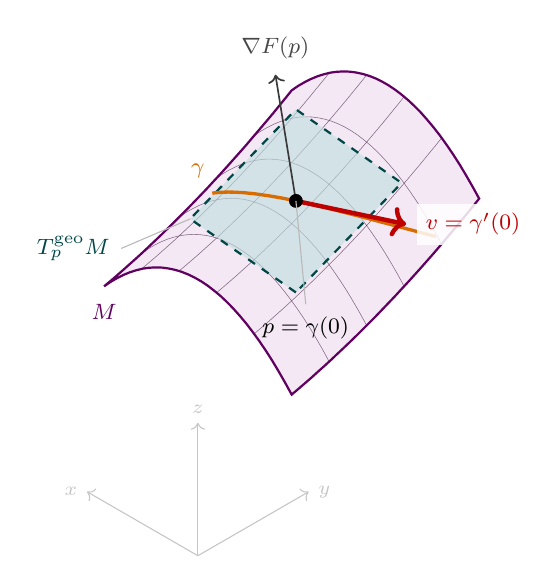
\begin{tikzpicture}[scale=1.25]
\draw[gray!45,->] (0,0) -- (-1.126,0.650) node[anchor=east,font=\scriptsize]{$x$};
\draw[gray!45,->] (0,0) -- (1.126,0.650) node[anchor=west,font=\scriptsize]{$y$};
\draw[gray!45,->] (0,0) -- (0.000,1.350) node[anchor=south,font=\scriptsize]{$z$};
\fill[violet!9] (0.953,1.637) -- (1.018,1.692) -- (1.084,1.749) -- (1.150,1.806) -- (1.215,1.865) -- (1.281,1.924) -- (1.347,1.984) -- (1.412,2.046) -- (1.478,2.108) -- (1.544,2.171) -- (1.610,2.235) -- (1.675,2.300) -- (1.741,2.366) -- (1.807,2.432) -- (1.872,2.500) -- (1.938,2.569) -- (2.004,2.638) -- (2.069,2.709) -- (2.135,2.780) -- (2.201,2.853) -- (2.267,2.926) -- (2.332,3.000) -- (2.398,3.075) -- (2.464,3.152) -- (2.529,3.229) -- (2.595,3.307) -- (2.661,3.385) -- (2.726,3.465) -- (2.792,3.546) -- (2.858,3.628) -- (2.858,3.628) -- (2.792,3.748) -- (2.726,3.863) -- (2.661,3.972) -- (2.595,4.075) -- (2.529,4.172) -- (2.464,4.263) -- (2.398,4.348) -- (2.332,4.427) -- (2.267,4.501) -- (2.201,4.568) -- (2.135,4.630) -- (2.069,4.685) -- (2.004,4.735) -- (1.938,4.779) -- (1.872,4.817) -- (1.807,4.849) -- (1.741,4.875) -- (1.675,4.895) -- (1.610,4.909) -- (1.544,4.918) -- (1.478,4.920) -- (1.412,4.917) -- (1.347,4.908) -- (1.281,4.892) -- (1.215,4.871) -- (1.150,4.844) -- (1.084,4.811) -- (1.018,4.773) -- (0.953,4.728) -- (0.953,4.728) -- (0.887,4.646) -- (0.821,4.565) -- (0.756,4.485) -- (0.690,4.407) -- (0.624,4.329) -- (0.558,4.252) -- (0.493,4.175) -- (0.427,4.100) -- (0.361,4.026) -- (0.296,3.953) -- (0.230,3.880) -- (0.164,3.809) -- (0.099,3.738) -- (0.033,3.669) -- (-0.033,3.600) -- (-0.099,3.532) -- (-0.164,3.466) -- (-0.230,3.400) -- (-0.296,3.335) -- (-0.361,3.271) -- (-0.427,3.208) -- (-0.493,3.146) -- (-0.558,3.084) -- (-0.624,3.024) -- (-0.690,2.965) -- (-0.756,2.906) -- (-0.821,2.849) -- (-0.887,2.792) -- (-0.953,2.737) -- (-0.953,2.737) -- (-0.887,2.782) -- (-0.821,2.820) -- (-0.756,2.853) -- (-0.690,2.880) -- (-0.624,2.901) -- (-0.558,2.917) -- (-0.493,2.926) -- (-0.427,2.929) -- (-0.361,2.927) -- (-0.296,2.918) -- (-0.230,2.904) -- (-0.164,2.884) -- (-0.099,2.858) -- (-0.033,2.826) -- (0.033,2.788) -- (0.099,2.744) -- (0.164,2.694) -- (0.230,2.639) -- (0.296,2.577) -- (0.361,2.510) -- (0.427,2.436) -- (0.493,2.357) -- (0.558,2.272) -- (0.624,2.181) -- (0.690,2.084) -- (0.756,1.981) -- (0.821,1.872) -- (0.887,1.757) -- (0.953,1.637) -- cycle;
\draw[violet!28!black,very thin,opacity=0.55] (1.334,1.972) -- (1.268,2.093) -- (1.202,2.208) -- (1.137,2.316) -- (1.071,2.419) -- (1.005,2.516) -- (0.939,2.607) -- (0.874,2.692) -- (0.808,2.772) -- (0.742,2.845) -- (0.677,2.913) -- (0.611,2.974) -- (0.545,3.030) -- (0.480,3.079) -- (0.414,3.123) -- (0.348,3.161) -- (0.282,3.193) -- (0.217,3.219) -- (0.151,3.240) -- (0.085,3.254) -- (0.020,3.262) -- (-0.046,3.265) -- (-0.112,3.261) -- (-0.177,3.252) -- (-0.243,3.237) -- (-0.309,3.216) -- (-0.374,3.189) -- (-0.440,3.156) -- (-0.506,3.117) -- (-0.572,3.072);
\draw[violet!28!black,very thin,opacity=0.55] (1.715,2.339) -- (1.649,2.460) -- (1.583,2.574) -- (1.518,2.683) -- (1.452,2.786) -- (1.386,2.883) -- (1.321,2.974) -- (1.255,3.059) -- (1.189,3.139) -- (1.123,3.212) -- (1.058,3.279) -- (0.992,3.341) -- (0.926,3.397) -- (0.861,3.446) -- (0.795,3.490) -- (0.729,3.528) -- (0.664,3.560) -- (0.598,3.586) -- (0.532,3.606) -- (0.466,3.621) -- (0.401,3.629) -- (0.335,3.632) -- (0.269,3.628) -- (0.204,3.619) -- (0.138,3.604) -- (0.072,3.583) -- (0.007,3.556) -- (-0.059,3.523) -- (-0.125,3.484) -- (-0.191,3.439);
\draw[violet!28!black,very thin,opacity=0.55] (2.096,2.737) -- (2.030,2.858) -- (1.964,2.973) -- (1.899,3.081) -- (1.833,3.184) -- (1.767,3.281) -- (1.702,3.372) -- (1.636,3.457) -- (1.570,3.537) -- (1.504,3.610) -- (1.439,3.678) -- (1.373,3.739) -- (1.307,3.795) -- (1.242,3.844) -- (1.176,3.888) -- (1.110,3.926) -- (1.045,3.958) -- (0.979,3.984) -- (0.913,4.005) -- (0.847,4.019) -- (0.782,4.027) -- (0.716,4.030) -- (0.650,4.026) -- (0.585,4.017) -- (0.519,4.002) -- (0.453,3.981) -- (0.388,3.954) -- (0.322,3.921) -- (0.256,3.882) -- (0.191,3.837);
\draw[violet!28!black,very thin,opacity=0.55] (2.477,3.167) -- (2.411,3.287) -- (2.345,3.402) -- (2.280,3.511) -- (2.214,3.614) -- (2.148,3.711) -- (2.083,3.802) -- (2.017,3.887) -- (1.951,3.966) -- (1.885,4.040) -- (1.820,4.107) -- (1.754,4.169) -- (1.688,4.224) -- (1.623,4.274) -- (1.557,4.318) -- (1.491,4.356) -- (1.426,4.388) -- (1.360,4.414) -- (1.294,4.434) -- (1.229,4.448) -- (1.163,4.457) -- (1.097,4.459) -- (1.031,4.456) -- (0.966,4.447) -- (0.900,4.431) -- (0.834,4.410) -- (0.769,4.383) -- (0.703,4.350) -- (0.637,4.312) -- (0.572,4.267);
\draw[violet!28!black,very thin,opacity=0.55] (0.572,2.254) -- (0.637,2.310) -- (0.703,2.366) -- (0.769,2.424) -- (0.834,2.482) -- (0.900,2.541) -- (0.966,2.602) -- (1.031,2.663) -- (1.097,2.725) -- (1.163,2.788) -- (1.229,2.852) -- (1.294,2.917) -- (1.360,2.983) -- (1.426,3.050) -- (1.491,3.117) -- (1.557,3.186) -- (1.623,3.256) -- (1.688,3.326) -- (1.754,3.398) -- (1.820,3.470) -- (1.885,3.543) -- (1.951,3.617) -- (2.017,3.693) -- (2.083,3.769) -- (2.148,3.846) -- (2.214,3.924) -- (2.280,4.003) -- (2.345,4.083) -- (2.411,4.163) -- (2.477,4.245);
\draw[violet!28!black,very thin,opacity=0.55] (0.191,2.673) -- (0.256,2.728) -- (0.322,2.785) -- (0.388,2.842) -- (0.453,2.901) -- (0.519,2.960) -- (0.585,3.020) -- (0.650,3.081) -- (0.716,3.144) -- (0.782,3.207) -- (0.847,3.271) -- (0.913,3.336) -- (0.979,3.401) -- (1.045,3.468) -- (1.110,3.536) -- (1.176,3.605) -- (1.242,3.674) -- (1.307,3.745) -- (1.373,3.816) -- (1.439,3.889) -- (1.504,3.962) -- (1.570,4.036) -- (1.636,4.111) -- (1.702,4.187) -- (1.767,4.264) -- (1.833,4.342) -- (1.899,4.421) -- (1.964,4.501) -- (2.030,4.582) -- (2.096,4.664);
\draw[violet!28!black,very thin,opacity=0.55] (-0.191,2.893) -- (-0.125,2.948) -- (-0.059,3.005) -- (0.007,3.062) -- (0.072,3.121) -- (0.138,3.180) -- (0.204,3.240) -- (0.269,3.301) -- (0.335,3.364) -- (0.401,3.427) -- (0.466,3.491) -- (0.532,3.556) -- (0.598,3.621) -- (0.664,3.688) -- (0.729,3.756) -- (0.795,3.825) -- (0.861,3.894) -- (0.926,3.965) -- (0.992,4.036) -- (1.058,4.109) -- (1.123,4.182) -- (1.189,4.256) -- (1.255,4.331) -- (1.321,4.407) -- (1.386,4.484) -- (1.452,4.562) -- (1.518,4.641) -- (1.583,4.721) -- (1.649,4.802) -- (1.715,4.884);
\draw[violet!28!black,very thin,opacity=0.55] (-0.572,2.914) -- (-0.506,2.970) -- (-0.440,3.026) -- (-0.374,3.084) -- (-0.309,3.142) -- (-0.243,3.201) -- (-0.177,3.262) -- (-0.112,3.323) -- (-0.046,3.385) -- (0.020,3.448) -- (0.085,3.512) -- (0.151,3.577) -- (0.217,3.643) -- (0.282,3.710) -- (0.348,3.777) -- (0.414,3.846) -- (0.480,3.916) -- (0.545,3.986) -- (0.611,4.058) -- (0.677,4.130) -- (0.742,4.203) -- (0.808,4.277) -- (0.874,4.353) -- (0.939,4.429) -- (1.005,4.506) -- (1.071,4.584) -- (1.137,4.663) -- (1.202,4.743) -- (1.268,4.823) -- (1.334,4.905);
\draw[violet!75!black,thick] (0.953,1.637) -- (1.018,1.692) -- (1.084,1.749) -- (1.150,1.806) -- (1.215,1.865) -- (1.281,1.924) -- (1.347,1.984) -- (1.412,2.046) -- (1.478,2.108) -- (1.544,2.171) -- (1.610,2.235) -- (1.675,2.300) -- (1.741,2.366) -- (1.807,2.432) -- (1.872,2.500) -- (1.938,2.569) -- (2.004,2.638) -- (2.069,2.709) -- (2.135,2.780) -- (2.201,2.853) -- (2.267,2.926) -- (2.332,3.000) -- (2.398,3.075) -- (2.464,3.152) -- (2.529,3.229) -- (2.595,3.307) -- (2.661,3.385) -- (2.726,3.465) -- (2.792,3.546) -- (2.858,3.628) -- (2.858,3.628) -- (2.792,3.748) -- (2.726,3.863) -- (2.661,3.972) -- (2.595,4.075) -- (2.529,4.172) -- (2.464,4.263) -- (2.398,4.348) -- (2.332,4.427) -- (2.267,4.501) -- (2.201,4.568) -- (2.135,4.630) -- (2.069,4.685) -- (2.004,4.735) -- (1.938,4.779) -- (1.872,4.817) -- (1.807,4.849) -- (1.741,4.875) -- (1.675,4.895) -- (1.610,4.909) -- (1.544,4.918) -- (1.478,4.920) -- (1.412,4.917) -- (1.347,4.908) -- (1.281,4.892) -- (1.215,4.871) -- (1.150,4.844) -- (1.084,4.811) -- (1.018,4.773) -- (0.953,4.728) -- (0.953,4.728) -- (0.887,4.646) -- (0.821,4.565) -- (0.756,4.485) -- (0.690,4.407) -- (0.624,4.329) -- (0.558,4.252) -- (0.493,4.175) -- (0.427,4.100) -- (0.361,4.026) -- (0.296,3.953) -- (0.230,3.880) -- (0.164,3.809) -- (0.099,3.738) -- (0.033,3.669) -- (-0.033,3.600) -- (-0.099,3.532) -- (-0.164,3.466) -- (-0.230,3.400) -- (-0.296,3.335) -- (-0.361,3.271) -- (-0.427,3.208) -- (-0.493,3.146) -- (-0.558,3.084) -- (-0.624,3.024) -- (-0.690,2.965) -- (-0.756,2.906) -- (-0.821,2.849) -- (-0.887,2.792) -- (-0.953,2.737) -- (-0.953,2.737) -- (-0.887,2.782) -- (-0.821,2.820) -- (-0.756,2.853) -- (-0.690,2.880) -- (-0.624,2.901) -- (-0.558,2.917) -- (-0.493,2.926) -- (-0.427,2.929) -- (-0.361,2.927) -- (-0.296,2.918) -- (-0.230,2.904) -- (-0.164,2.884) -- (-0.099,2.858) -- (-0.033,2.826) -- (0.033,2.788) -- (0.099,2.744) -- (0.164,2.694) -- (0.230,2.639) -- (0.296,2.577) -- (0.361,2.510) -- (0.427,2.436) -- (0.493,2.357) -- (0.558,2.272) -- (0.624,2.181) -- (0.690,2.084) -- (0.756,1.981) -- (0.821,1.872) -- (0.887,1.757) -- (0.953,1.637) -- cycle;
\fill[teal!25,opacity=0.62] (0.996,2.675) -- (-0.078,3.422) -- (0.996,4.535) -- (2.070,3.787) -- cycle;
\draw[teal!55!black,dashed,thick] (0.996,2.675) -- (-0.078,3.422) -- (0.996,4.535) -- (2.070,3.787) -- cycle;
\draw[orange!85!black,very thick] (0.146,3.683) -- (0.162,3.686) -- (0.179,3.688) -- (0.197,3.689) -- (0.215,3.691) -- (0.233,3.692) -- (0.252,3.693) -- (0.272,3.694) -- (0.292,3.694) -- (0.312,3.695) -- (0.333,3.694) -- (0.355,3.694) -- (0.376,3.693) -- (0.399,3.692) -- (0.422,3.691) -- (0.445,3.690) -- (0.469,3.688) -- (0.493,3.686) -- (0.518,3.683) -- (0.543,3.681) -- (0.569,3.678) -- (0.595,3.675) -- (0.622,3.671) -- (0.649,3.667) -- (0.677,3.663) -- (0.705,3.659) -- (0.733,3.655) -- (0.762,3.650) -- (0.792,3.645) -- (0.822,3.639) -- (0.853,3.634) -- (0.884,3.628) -- (0.915,3.621) -- (0.947,3.615) -- (0.979,3.608) -- (1.012,3.601) -- (1.046,3.594) -- (1.080,3.587) -- (1.114,3.579) -- (1.149,3.571) -- (1.184,3.563) -- (1.220,3.554) -- (1.257,3.546) -- (1.293,3.537) -- (1.331,3.528) -- (1.368,3.519) -- (1.407,3.509) -- (1.445,3.499) -- (1.485,3.489) -- (1.524,3.479) -- (1.564,3.469) -- (1.605,3.458) -- (1.646,3.448) -- (1.688,3.437) -- (1.730,3.426) -- (1.772,3.414) -- (1.815,3.403) -- (1.859,3.391) -- (1.903,3.380) -- (1.948,3.368) -- (1.992,3.356) -- (2.038,3.344) -- (2.084,3.332) -- (2.130,3.319) -- (2.177,3.307) -- (2.225,3.294) -- (2.272,3.281) -- (2.321,3.269) -- (2.370,3.256) -- (2.419,3.243);
\draw[gray!45!black,->,semithick] (0.996,3.605) -- (0.788,4.887);
\node[gray!55!black,font=\footnotesize,anchor=south] at (0.788,4.947) {$\nabla F(p)$};
\draw[red!75!black,->,ultra thick] (0.996,3.605) -- (2.116,3.368);
\fill[black] (0.996,3.605) circle (2.0pt);
\node[fill=white, fill opacity=0.85, text opacity=1, text=red!75!black,font=\footnotesize,anchor=west] at (2.216,3.368) {$v=\gamma'(0)$};
\draw[gray!55,thin] (-0.078,3.422) -- (-0.778,3.122);
\node[teal!55!black,font=\footnotesize,anchor=east] at (-0.798,3.122) {$T^{\geo}_pM$};
\node[orange!85!black,font=\footnotesize,anchor=south east] at (0.166,3.743) {$\gamma$};
\draw[gray!55,thin] (0.996,3.605) -- (1.096,2.555);
\node[font=\footnotesize,anchor=north] at (1.096,2.525) {$p=\gamma(0)$};
\node[violet!75!black,font=\footnotesize,anchor=north] at (-0.953,2.657) {$M$};
\end{tikzpicture}
\end{center}

``Smooth'' for $\gamma$ means smooth as a map into the Euclidean space $\mathbb{R}^{n+k}$; the constraint that it take values in $M$ is a separate condition. The derivative $\gamma'(0)$ is computed with the vector space structure of $\mathbb{R}^{n+k}$, which is exactly what an abstract manifold lacks. The figure shows the definition: a curve $\gamma$ drawn on $M$ through $p$, its velocity $v$ at $t=0$ (a vector of the ambient space, drawn from $p$), and the plane these velocities sweep out as $\gamma$ ranges over all such curves --- which Theorem~\ref{thm:tangent-kernel} identifies as $\ker F'(p)$, and which is therefore orthogonal to the gradient $\nabla F(p)$, shown in grey for contrast. Note that $T^{\geo}_pM$ is drawn as a plane through $p$ only as an aid: as a subspace of $\mathbb{R}^{n+k}$ it passes through the origin, and it is the \emph{translate} to $p$ that is tangent to $M$.

It is not obvious from Definition~\ref{def:geometric-tangent} that $T^{\geo}_pM$ is closed under addition: given two curves through $p$ with velocities $v$ and $w$, there is no evident curve with velocity $v + w$. ``How do I add two curves?'' Both this and the dimension follow from an algebraic description.

\begin{lembox}[Locality of the Geometric Tangent Space]\thmlabel{lem:tangent-local}
If $M' \subseteq M$ is open in $M$ and $p \in M'$, then $T^{\geo}_pM' = T^{\geo}_pM$.
\end{lembox}

\begin{proof}
$\subseteq$ is clear, a curve in $M'$ being a curve in $M$. For $\supseteq$, let $\gamma : (-\varepsilon,\varepsilon) \to M$ be smooth with $\gamma(0) = p$. Since $\gamma$ is continuous and $M'$ is open in $M$, the set $\gamma^{-1}(M')$ is open in $(-\varepsilon,\varepsilon)$ and contains $0$, so it contains an interval $(-\delta,\delta)$. The restriction $\gamma|_{(-\delta,\delta)}$ takes values in $M'$ and has the same velocity at $0$.
\end{proof}

\begin{lembox}[The Geometric Tangent Space of a Graph]\thmlabel{lem:tangent-graph}
Let $A \subseteq \mathbb{R}^n$ be open, $G : A \to \mathbb{R}^k$ smooth, and
\[
M = \{\, (x, G(x)) \mid x \in A \,\} \subseteq \mathbb{R}^{n+k}
\]
its graph. For $p = (x_0, G(x_0))$ with $x_0 \in A$,
\[
T^{\geo}_pM \;=\; \{\, (u,\; G'(x_0)\,u) \mid u \in \mathbb{R}^n \,\},
\]
the graph of the linear map $G'(x_0) : \mathbb{R}^n \to \mathbb{R}^k$. In particular $T^{\geo}_pM$ is a linear subspace of $\mathbb{R}^{n+k}$ of dimension $n$.
\end{lembox}

\begin{proof}
\textit{(Set in Lecture~8 as an exercise --- ``not a trivial exercise''; filled in.)} $\subseteq$: let $\gamma : (-\varepsilon,\varepsilon) \to M$ be smooth with $\gamma(0) = p$, and write $\gamma = (\gamma_1, \gamma_2)$ with $\gamma_1$ into $\mathbb{R}^n$ and $\gamma_2$ into $\mathbb{R}^k$. Both components are smooth, and since $\gamma(t) \in M$ for every $t$ we have $\gamma_2 = G \circ \gamma_1$ and $\gamma_1(0) = x_0$. By the chain rule
\[
\gamma'(0) = \big(\gamma_1'(0),\; G'(x_0)\,\gamma_1'(0)\big),
\]
which lies in the graph of $G'(x_0)$.

$\supseteq$: given $u \in \mathbb{R}^n$, choose $\varepsilon > 0$ with $x_0 + tu \in A$ for $|t| < \varepsilon$, possible since $A$ is open, and set
\[
\gamma(t) = \big(x_0 + tu,\; G(x_0 + tu)\big).
\]
This is smooth into $\mathbb{R}^{n+k}$, takes values in $M$, has $\gamma(0) = p$, and $\gamma'(0) = (u, G'(x_0)u)$ by the chain rule.

Finally, the graph of a linear map $\mathbb{R}^n \to \mathbb{R}^k$ is a linear subspace of $\mathbb{R}^{n+k}$, and $u \mapsto (u, G'(x_0)u)$ is an injective linear map onto it, so its dimension is $n$.
\end{proof}

\begin{rembox}\label{rem:tangent-2}
Uribe stated this lemma and left it as an exercise, calling it ``not a trivial exercise''; the proof above is short but both inclusions are needed, and the $\supseteq$ half --- lifting a straight line from the chart --- is the construction that reappears in \S\ref{sub:derivations-motivation} as the curve defining $D_v$. In words: \emph{the geometric tangent space to a graph is the graph of the differential.}
\end{rembox}

\begin{thmbox}[The Geometric Tangent Space Is the Kernel of the Jacobian]\thmlabel{thm:tangent-kernel}
$T^{\geo}_pM = \ker F'(p)$, where $F'(p) : \mathbb{R}^{n+k} \to \mathbb{R}^k$ is the Jacobian at $p$. In particular $T^{\geo}_pM$ is a linear subspace of $\mathbb{R}^{n+k}$ of dimension $n = \dim M$.
\leeref{Proposition 5.38}
\end{thmbox}

\begin{proof}
The order is Lecture~8's sketch, which built on an inclusion proved in Lecture~7.

\emph{1. The inclusion (Lecture~7: ``last time we saw this inclusion'').} $T^{\geo}_pM \subseteq \ker F'(p)$. Let $v \in T^{\geo}_pM$ with $\gamma$ as in Definition~\ref{def:geometric-tangent}. The composite $F \circ \gamma : (-\varepsilon,\varepsilon) \to \mathbb{R}^k$ is smooth, being a composite of smooth maps between Euclidean spaces, and since $\gamma(t) \in M = F^{-1}(c)$ for every $t$ it is the constant $c$. Differentiating at $t = 0$ and applying the chain rule,
\[
\vec 0 = \frac{d}{dt}\Big|_{t=0} F(\gamma(t)) = F'(\gamma(0))\,\gamma'(0) = F'(p)\, v ,
\]
so $v \in \ker F'(p)$.

\emph{2. Everything is local near $p$, so WLOG $M$ is a graph.} ``Since everything is local near $p$ \ldots\ these regular level sets are locally graphs of functions, for various choices of variables.'' \textit{(Completion.)} By the proof of Theorem~\ref{thm:regular-value}, after permuting coordinates there is an open box $V \times V'$ containing $p$ and a smooth $G : V \to V'$ with $M \cap (V \times V') = \{(x, G(x)) \mid x \in V\}$. By Lemma~\ref{lem:tangent-local} the geometric tangent space is unchanged on passing to this open piece.

\emph{3. The claim: the tangent space to a graph is the graph of the derivative.} $T^{\geo}_pM$ is the graph of $G'(x_0)$, where $p = (x_0, G(x_0))$ --- set in lecture as ``not a trivial exercise'' and proved in Lemma~\ref{lem:tangent-graph}. So $T^{\geo}_pM$ is a subspace of dimension $n$.

\emph{4. The kernel has dimension $n$, by rank--nullity.} Since $c$ is a regular value, $F'(p) : \mathbb{R}^{n+k} \to \mathbb{R}^k$ has rank $k$, so rank--nullity gives $\dim \ker F'(p) = (n+k) - k = n$.

\emph{5. ``We must have equality.''} $T^{\geo}_pM$ is an $n$-dimensional subspace contained in the $n$-dimensional subspace $\ker F'(p)$, so the two are equal.
\end{proof}

\begin{rembox}\label{rem:tangent-3}
The structure is worth noticing, because it is not the obvious one. Only the \emph{easy} inclusion is proved directly; the reverse inclusion is never constructed, but forced by a dimension count. Uribe: ``it's best actually to prove something else'' --- namely the graph lemma, from which both the vector space structure and the dimension of $T^{\geo}_pM$ are immediate, after which ``we must have equality.''
\end{rembox}

\begin{corbox}[Three Descriptions of the Geometric Tangent Space]\thmlabel{cor:tangent-three}
In the notation of the proof, with $\alpha : V \to \mathbb{R}^{n+k}$, $\alpha(x) = (x, h(x))$ the parametrization inverse to the graph chart,
\[
T^{\geo}_pM \;=\; \{\text{velocities of curves in } M \text{ through } p\} \;=\; \ker F'(p) \;=\; \operatorname{im} D\alpha_a ,
\]
and $D\alpha_a : \mathbb{R}^n \to \mathbb{R}^{n+k}$, $u \mapsto (u, Dh_a u)$, is an isomorphism onto $T^{\geo}_pM$.
\leeref{Propositions 5.37 and 5.38}
\end{corbox}

\begin{proof}
The first equality is the definition and the second is Theorem~\ref{thm:tangent-kernel}. Step 2 of that proof shows every $v \in \ker F'(p)$ has the form $(v_1, Dh_a v_1) = D\alpha_a(v_1)$, so $\ker F'(p) \subseteq \operatorname{im} D\alpha_a$; and differentiating $F \circ \alpha \equiv c$ gives $F'(p) \circ D\alpha_a = 0$, so $\operatorname{im} D\alpha_a \subseteq \ker F'(p)$. $D\alpha_a$ is injective because its first $n$ components are the identity, and both spaces have dimension $n$.
\end{proof}

\begin{rembox}\label{rem:tangent-4}
The corollary is the infinitesimal form of \S\ref{sub:ext-int}: the geometric tangent space can be read off from the \emph{external} description as the kernel of the constraint map, or from the \emph{internal} description as the image of the derivative of a parametrization, and the two agree. The geometric definition, via curves, is the one that makes no reference to either presentation --- which is why it is the one that will generalize.
\end{rembox}

\subsection{Examples}

\begin{exbox}[The Sphere]\exlabel{ex:tangent-sphere}
For $S^n = F^{-1}(1)$ with $F(x) = |x|^2 = \sum x_i^2$ on $\mathbb{R}^{n+1}$, the Jacobian at $p$ is the row vector $F'(p) = 2p^{\mathsf T}$, and $1$ is a regular value since $p \neq 0$ on $S^n$. Hence
\[
T^{\geo}_pS^n = \ker\big(2p^{\mathsf T}\big) = \{\, v \in \mathbb{R}^{n+1} \mid p \cdot v = 0 \,\} = p^{\perp},
\]
the hyperplane orthogonal to the position vector --- the tangent plane of calculus, now as a theorem. Directly from the definition: any curve $\gamma$ on the sphere satisfies $\gamma(t)\cdot\gamma(t) = 1$, so $2\,\gamma(t)\cdot\gamma'(t) = 0$, and at $t = 0$ this is $p \cdot v = 0$.
\end{exbox}

The sphere through the course: a topological manifold with hemisphere charts in Section~\ref{sec:ex-spheres}; the homogeneous space $\SO(3)/\SO(2)$ in Example~\ref{ex:s2-homogeneous}; the Riemann sphere $\mathbb{CP}^1$ in Proposition~\ref{prop:cp1-sphere}; its geometric tangent spaces in Example~\ref{ex:tangent-sphere} and its transverse intersection with a plane in Example~\ref{ex:sphere-plane-transverse}; the double cover $S^n \to \mathbb{RP}^n$ and the Hopf fibration $S^{2n+1} \to \mathbb{CP}^n$ in Section~\ref{sec:ex-hopf}; and $S^3 = \mathrm{SU}(2)$ in Proposition~\ref{prop:s3-su2}.


\begin{exbox}[The Orthogonal Group]\exlabel{ex:tangent-On}
For $\Ogp(n) = F^{-1}(I)$ with $F : \Mat(n,\mathbb{R}) \to \Sym(n,\mathbb{R})$, $F(g) = gg^{\mathsf T}$, Theorem~\ref{thm:tangent-kernel} applies after identifying both spaces with Euclidean spaces by linear coordinates, under which the Jacobian corresponds to the differential $dF_g$ of Definition~\ref{def:vs-differential}. Proposition~\ref{prop:On-kernel} then gives
\[
T^{\geo}_g\Ogp(n) = \ker dF_g = g \cdot \Skew(n,\mathbb{R}), \qquad T^{\geo}_I \Ogp(n) = \Skew(n,\mathbb{R}),
\]
of dimension $\tfrac{n(n-1)}{2}$, as it must be. Directly from the definition, at $g = I$: if $\gamma$ is a curve of orthogonal matrices with $\gamma(0) = I$, then $\gamma(t)\gamma(t)^{\mathsf T} = I$ for all $t$; differentiating at $0$ gives $\gamma'(0) + \gamma'(0)^{\mathsf T} = 0$, so the velocity is skew-symmetric. This geometric tangent space at the identity is the object that will later be called the \emph{Lie algebra} $\mathfrak{so}(n)$.
\end{exbox}

\begin{rembox}\label{rem:tangent-5}
For $\Ogp(n)$ the ambient space is $\Mat(n,\mathbb{R})$ rather than $\mathbb{R}^{n^2}$; Definition~\ref{def:geometric-tangent} is used in its vector-space form, and Theorem~\ref{thm:tangent-kernel} transfers across the linear isomorphism of Proposition~\ref{prop:vs-manifold}. The description $T^{\geo}_g\Ogp(n) = g \cdot T^{\geo}_I\Ogp(n)$ --- every geometric tangent space is a translate of the one at the identity --- is the first sign that a group structure simplifies the tangent bundle; it will be a general fact about Lie groups.
\end{rembox}

\begin{exbox}[The Unitary Group]\exlabel{ex:tangent-Un}
By Proposition~\ref{prop:Un-kernel} and Theorem~\ref{thm:tangent-kernel} (transferred to the real vector space $\Mat(n,\mathbb{C})$ as in the note above),
\[
T^{\geo}_g\Ugp(n) = \ker dF_g = \mathfrak{u}(n)\cdot g = g\cdot\mathfrak{u}(n), \qquad T^{\geo}_I\Ugp(n) = \mathfrak{u}(n).
\]
Directly from the definition at $g = I$: a curve of unitary matrices with $\gamma(0) = I$ satisfies $\gamma(t)\gamma(t)^* = I$, and differentiating at $0$ gives $\gamma'(0) + \gamma'(0)^* = 0$.
\end{exbox}

\begin{thmbox}[The Classical Groups]\thmlabel{thm:classical-summary}
Each classical group of Theorem~\ref{thm:classical-manifolds} is a smooth manifold, of the dimension and with the geometric tangent space at the identity given below. Moreover, for $G = \SL(n,\mathbb{R}), \Ogp(n), \SO(n), \Ugp(n)$ and every $g \in G$,
\[
T^{\geo}_g G \;=\; g \cdot T^{\geo}_I G \;=\; T^{\geo}_I G \cdot g .
\]
\leeref{Examples 7.27--7.30}
\end{thmbox}

\begin{center}
\renewcommand{\arraystretch}{1.35}
\begin{tabular}{l l c l}
\hline
Group $G$ & Presentation & $\dim G$ & $T^{\geo}_I G$ \\
\hline
$\GL(n,\mathbb{R})$ & open in $\Mat(n,\mathbb{R})$ & $n^2$ & $\Mat(n,\mathbb{R})$ \\
$\GL(n,\mathbb{C})$ & open in $\Mat(n,\mathbb{C})$ & $2n^2$ & $\Mat(n,\mathbb{C})$ \\
$\SL(n,\mathbb{R})$ & $\det^{-1}(1)$ & $n^2 - 1$ & $\mathfrak{sl}(n) = \{A \mid \tr A = 0\}$ \\
$\Ogp(n)$ & $F^{-1}(I)$, $F(g) = gg^{\mathsf T} \in \Sym(n,\mathbb{R})$ & $\tfrac{n(n-1)}{2}$ & $\mathfrak{so}(n) = \Skew(n,\mathbb{R})$ \\
$\SO(n)$ & open in $\Ogp(n)$ & $\tfrac{n(n-1)}{2}$ & $\mathfrak{so}(n)$ \\
$\Ugp(n)$ & $F^{-1}(I)$, $F(g) = gg^* \in \Herm(n)$ & $n^2$ & $\mathfrak{u}(n) = \{X \mid X^* = -X\}$ \\
\hline
\end{tabular}
\end{center}

\begin{proof}
\emph{The general linear groups.} An open subset $U$ of a finite-dimensional vector space $V$ is a smooth manifold of dimension $\dim V$ (one chart, the restriction of a linear chart). Definition~\ref{def:geometric-tangent} makes sense verbatim for $U \subseteq V$, and every $v \in V$ is the velocity of the curve $t \mapsto p + tv$, which stays in $U$ for small $|t|$; so $T^{\geo}_pU = V$.

\emph{$\SL(n,\mathbb{R})$.} Smoothness and dimension are Corollary~\ref{prop:SL-loc-euc} with Proposition~\ref{prop:level-set-smooth}. By Proposition~\ref{prop:jacobi}, $d(\det)_g(A) = \det(g)\,\tr(g^{-1}A)$, so for $g \in \SL(n,\mathbb{R})$ Theorem~\ref{thm:tangent-kernel} gives $T^{\geo}_g\SL = \{A \mid \tr(g^{-1}A) = 0\}$. Writing $A = gB$ this is $g\cdot\mathfrak{sl}(n)$; writing $A = Bg$ and using $\tr(g^{-1}Bg) = \tr B$, it is $\mathfrak{sl}(n)\cdot g$. The trace condition removes one dimension, consistently with $n^2 - 1$.

\emph{$\Ogp(n)$ and $\SO(n)$.} Example~\ref{ex:On-smooth}, Corollary~\ref{cor:On-consequences}, and Example~\ref{ex:tangent-On}; since $\SO(n)$ is open in $\Ogp(n)$ its geometric tangent spaces are those of $\Ogp(n)$ (Lemma~\ref{lem:tangent-local}). For the right translate, $\Skew(n,\mathbb{R})$ is preserved by conjugation by orthogonal $g$, exactly as in the proof of Proposition~\ref{prop:Un-kernel}.

\emph{$\Ugp(n)$.} Example~\ref{ex:Un-smooth} and Example~\ref{ex:tangent-Un}.
\end{proof}

\begin{defbox}[Adjoint Action]\deflabel{def:adjoint}
Let $G$ be one of $\SL(n,\mathbb{R})$, $\Ogp(n)$, $\SO(n)$, $\Ugp(n)$, and $\mathfrak{g} = T^{\geo}_I G$. For $g \in G$, \textbf{conjugation} by $g$ is $\mathrm{Ad}_g(X) = gXg^{-1}$. The \textbf{adjoint action} of $G$ on $\mathfrak{g}$ is $g \mapsto \mathrm{Ad}_g|_{\mathfrak{g}}$; that each $\mathrm{Ad}_g$ maps $\mathfrak{g}$ onto itself is part of the next proposition.
\end{defbox}

\begin{propbox}[The Adjoint Action]\thmlabel{prop:adjoint}
Let $G$ be one of $\SL(n,\mathbb{R})$, $\Ogp(n)$, $\SO(n)$, $\Ugp(n)$, and $\mathfrak{g} = T^{\geo}_I G$. For $g \in G$ the conjugation
\[
\mathrm{Ad}_g : \mathfrak{g} \to \mathfrak{g}, \qquad \mathrm{Ad}_g(X) = gXg^{-1},
\]
is a linear isomorphism, with $\mathrm{Ad}_{gh} = \mathrm{Ad}_g \circ \mathrm{Ad}_h$. Left and right multiplication $L_g(X) = gX$ and $R_g(X) = Xg$ satisfy $L_g = R_g \circ \mathrm{Ad}_g$.
\end{propbox}

\begin{proof}
That $\mathrm{Ad}_g$ maps $\mathfrak{g}$ into itself is checked case by case, with $\mathfrak{g}$ as in Theorem~\ref{thm:classical-summary}. For $\mathfrak{sl}(n)$: $\tr(gXg^{-1}) = \tr X$. For $g$ orthogonal and $X$ skew: $(gXg^{-1})^{\mathsf T} = (gXg^{\mathsf T})^{\mathsf T} = gX^{\mathsf T}g^{\mathsf T} = -gXg^{-1}$. For $g$ unitary and $X$ skew-Hermitian: $(gXg^*)^* = gX^*g^* = -gXg^{-1}$. $\mathrm{Ad}_g$ is linear, $\mathrm{Ad}_{gh}X = ghXh^{-1}g^{-1} = \mathrm{Ad}_g(\mathrm{Ad}_h X)$, and $\mathrm{Ad}_{g^{-1}}$ is an inverse. Finally $R_g(\mathrm{Ad}_g X) = gXg^{-1}g = gX$.
\end{proof}

\begin{rembox}[Left and Right Translates]\label{rem:left-right-translates}
The notes computed $T^{\geo}_g\Ogp(n) = g\cdot\Skew(n)$ by writing $A = gB$ (Proposition~\ref{prop:On-kernel}); Assignment~2 computed $T^{\geo}_g\Ugp(n) = \mathfrak{u}(n)\cdot g$ by writing $h = Xg$. Neither choice is privileged, and by the proposition the two agree, $g \cdot \mathfrak{g} = \mathrm{Ad}_g(\mathfrak{g}) \cdot g = \mathfrak{g} \cdot g$. This is the first structural fact about Lie groups to appear in the course: the geometric tangent space at the identity, carried to every other point by left or right multiplication, determines all the geometric tangent spaces. The spaces $\mathfrak{sl}(n)$, $\mathfrak{so}(n)$, $\mathfrak{u}(n)$ in the table will reappear as \emph{Lie algebras}.
\end{rembox}

\begin{center}
\begin{tikzcd}[row sep=2.8em, column sep=2.6em]
T^{\geo}_IG \arrow[rr, "\mathrm{Ad}_g \,:\, X \,\mapsto\, gXg^{-1}"] \arrow[dr, "L_g \,:\, X \,\mapsto\, gX"'] & & T^{\geo}_IG \arrow[dl, "R_g \,:\, X \,\mapsto\, Xg"] \\
& T^{\geo}_gG &
\end{tikzcd}
\end{center}

Left and right multiplication by $g$ both carry $T^{\geo}_IG$ isomorphically onto $T^{\geo}_gG$, and they differ by the adjoint action: $L_g = R_g \circ \mathrm{Ad}_g$, since $(gXg^{-1})g = gX$. The two descriptions of $T^{\geo}_gG$ agree precisely because $\mathrm{Ad}_g$ maps $T^{\geo}_IG$ onto itself.


\begin{defbox}[The Hat Map]\deflabel{def:hat-map}
The \textbf{hat map} $\mathbb{R}^3 \to \Skew(3,\mathbb{R})$ sends $v = (v_1, v_2, v_3)$ to
\[
\hat v = \begin{pmatrix} 0 & -v_3 & v_2 \\ v_3 & 0 & -v_1 \\ -v_2 & v_1 & 0 \end{pmatrix},
\]
a linear isomorphism, characterized by $\hat v\, x = v \times x$ for all $x \in \mathbb{R}^3$.
\end{defbox}

\begin{exbox}[$\SO(3)$ and Infinitesimal Rotations]\exlabel{ex:so3-infinitesimal}
$T^{\geo}_I\SO(3) = \Skew(3,\mathbb{R})$ is $3$-dimensional, and it is identified with $\mathbb{R}^3$ by the hat map of Definition~\ref{def:hat-map}
\[
v = (v_1,v_2,v_3) \longmapsto \hat v = \begin{pmatrix} 0 & -v_3 & v_2 \\ v_3 & 0 & -v_1 \\ -v_2 & v_1 & 0 \end{pmatrix},
\qquad \hat v\, x = v \times x .
\]
Every tangent vector at the identity is the velocity of a family of rotations. For the axis $e_3$,
\[
R(t) = \begin{pmatrix} \cos t & -\sin t & 0 \\ \sin t & \cos t & 0 \\ 0 & 0 & 1 \end{pmatrix}, \qquad R(0) = I, \qquad R'(0) = \begin{pmatrix} 0 & -1 & 0 \\ 1 & 0 & 0 \\ 0 & 0 & 0 \end{pmatrix} = \hat e_3 .
\]
For a unit vector $n$, choose $Q \in \SO(3)$ with $Qe_3 = n$ (possible by Example~\ref{ex:s2-homogeneous}); the rotation about $n$ by angle $t$ is $QR(t)Q^{\mathsf T}$, with velocity $Q\hat e_3 Q^{\mathsf T} = \widehat{Qe_3} = \hat n$ at $t = 0$, using the identity $\widehat{Qv} = Q\hat vQ^{\mathsf T}$ for $Q \in \SO(3)$, which holds because rotations preserve the cross product. Scaling the speed, every $\hat v$ is attained: \emph{a tangent vector to $\SO(3)$ at the identity is an angular velocity}, with direction the axis and length the rate of rotation.
\end{exbox}

\begin{rembox}\label{rem:tangent-6}
This connects the $\SO(3)$ material of \ref{sec:actions} and \ref{sec:homogeneous} with the geometric tangent space. The three dimensions of $\SO(3)$ are the two needed to specify an axis, a point of $S^2$, and one for the angle about it --- matching $S^2 \cong \SO(3)/\SO(2)$ of Example~\ref{ex:s2-homogeneous}, with the isotropy $\SO(2)$ being exactly the rotations about the fixed axis.
\end{rembox}

The classical groups through the course: defined in Section~\ref{sec:topgroups}, with the examples of Section~\ref{sec:ex-classical}; topological manifolds as level sets in Theorem~\ref{thm:classical-manifolds}; $\SO(2)$ and $\SO(3)$ acting on $\mathbb{R}^2$ and $\mathbb{R}^3$ in Examples~\ref{ex:so2-orbits} and~\ref{ex:so3-orbits}, and $\SO(3)$ on $S^2$ in Examples~\ref{ex:so3-isotropy} and~\ref{ex:s2-homogeneous}; $\Ogp(n)$ acting on the Grassmannians in Corollary~\ref{cor:grassmannian}; smooth manifolds in Examples~\ref{ex:On-smooth} and~\ref{ex:Un-smooth}; their tangent spaces at the identity in Theorem~\ref{thm:classical-summary}, with the infinitesimal rotations of Example~\ref{ex:so3-infinitesimal}; and the double cover $\mathrm{SU}(2) \to \SO(3)$ in Theorem~\ref{thm:double-cover}.


\begin{rembox}[Dimension Checks through Homogeneous Spaces]\label{rem:dimension-checks-through-homogeneous-spaces}
In every homogeneous space met so far, $\dim G/H = \dim G - \dim H$:
\begin{itemize}
    \item $S^2 = \SO(3)/\SO(2)$: \ $3 - 1 = 2$;
    \item $\Gr_k(\mathbb{R}^n) = \Ogp(n)/\big(\Ogp(k)\times\Ogp(n-k)\big)$: \ $\tfrac{n(n-1)}{2} - \tfrac{k(k-1)}{2} - \tfrac{(n-k)(n-k-1)}{2} = k(n-k)$;
    \item $S^{2n+1} = \Ugp(n+1)/\Ugp(n)$: \ $(n+1)^2 - n^2 = 2n+1$;
    \item $\mathbb{CP}^n = \Ugp(n+1)/\big(\Ugp(1)\times\Ugp(n)\big)$: \ $(n+1)^2 - 1 - n^2 = 2n$, the real dimension found from charts in Theorem~\ref{thm:cpn-atlas}.
\end{itemize}
The first two identifications are proved in \ref{sec:homogeneous}--\ref{sec:GH-topology}; the last two are their complex analogues --- $\Ugp(n+1)$ acts transitively on unit vectors of $\mathbb{C}^{n+1}$ and on complex lines --- and are not proved here. The formula itself is heuristic until quotient manifolds are available, when it becomes a theorem; for now it is a consistency check linking four separate computations.
\end{rembox}

\subsection{The Dimension of the Geometric Tangent Space}\label{sub:geo-dimension}

\begin{thmbox}[Dimension of the Geometric Tangent Space]\thmlabel{thm:geo-tangent-dimension}
Let $M = F^{-1}(c) \subseteq \mathbb{R}^{n+k}$ be as in Theorem~\ref{thm:tangent-kernel}, a manifold of dimension $n$. Then for every $p \in M$,
\[
\dim T^{\geo}_pM = n = \dim M .
\]
The geometric tangent space has the same dimension at every point, and it is the dimension of the manifold.
\end{thmbox}

\begin{proof}
\textit{(The last sentence of Theorem~\ref{thm:tangent-kernel}, recorded as a theorem in its own right.)} By Theorem~\ref{thm:tangent-kernel}, $T^{\geo}_pM = \ker F'(p)$. Since $c$ is a regular value, the $k \times (n+k)$ matrix $F'(p)$ has rank $k$, so by rank--nullity $\dim \ker F'(p) = (n + k) - k = n$.
\end{proof}

The count is the geometric meaning of ``$k$ independent equations in $n + k$ unknowns'': each equation removes one tangent direction, and $n$ remain at every point. Theorem~\ref{thm:tangent-dimension} gives the same number for the abstract tangent space, as it must, since the two spaces are isomorphic (Theorem~\ref{thm:ambient-abstract}).

\subsection{From Tangent Vectors to Derivations}\label{sub:derivations-motivation}

\textit{Motivation only; nothing in this subsection is used later, but it is where the abstract definition comes from.}

Keep $M = F^{-1}(c)$ and, by Lemmas \ref{lem:tangent-local} and \ref{lem:tangent-graph}, assume $M$ is the graph of a smooth $G : A \to \mathbb{R}^k$ over an open $A \subseteq \mathbb{R}^n$, with chart $\varphi : M \to A$ the projection $(x, G(x)) \mapsto x$ and $p = (x_0, G(x_0))$. Let $f : M \to \mathbb{R}$ be smooth, so that $f_\varphi = f \circ \varphi^{-1} : A \to \mathbb{R}$ is smooth (Definition~\ref{def:smooth-function}).

Given $v \in T^{\geo}_pM$, Lemma~\ref{lem:tangent-graph} provides a unique $u \in \mathbb{R}^n$ with $v = (u, G'(x_0)u)$. Lift the straight line $t \mapsto x_0 + tu$ from the chart to the manifold:
\[
\gamma(t) = \big(x_0 + tu,\; G(x_0 + tu)\big), \qquad \gamma(0) = p, \quad \gamma'(0) = v .
\]

\begin{center}
\begin{tikzcd}[row sep=3.0em, column sep=3.6em]
M \arrow[r, "f"] \arrow[d, shift right=0.6ex, "\varphi"'] & \mathbb{R} \\
A \subseteq \mathbb{R}^n \arrow[u, shift right=0.6ex, "\varphi^{-1}"'] \arrow[ur, "f_\varphi"'] &
\end{tikzcd}
\end{center}

The chart triangle for the graph case, as drawn on the board. Downstairs is the open set $A \subseteq \mathbb{R}^n$; upstairs is the manifold. The chart $\varphi(x, G(x)) = x$ and its inverse $\varphi^{-1}(x) = (x, G(x))$ pass between them, and the triangle commutes: $f = f_\varphi \circ \varphi$. Smoothness of $f$ \emph{means} smoothness of $f_\varphi$, so every computation with $f$ can be pushed downstairs, done in ordinary calculus, and read back. That is the manoeuvre in the next definition: the curve is built downstairs as a straight line, lifted upstairs by $\varphi^{-1}$, and the derivative taken downstairs again. ``Upstairs and downstairs are very useful terminologies.''

\begin{defbox}[The Directional Derivative Attached to a Tangent Vector]\deflabel{def:Dv}
Let $M \subseteq \mathbb{R}^{n+k}$ be the graph of a smooth $G : A \to \mathbb{R}^k$ on an open $A \subseteq \mathbb{R}^n$, with chart $\varphi(x, G(x)) = x$, and $p = (x_0, G(x_0))$. Let $v \in T^{\geo}_pM$, let $u \in \mathbb{R}^n$ be the vector with $v = (u, G'(x_0)u)$ (Lemma~\ref{lem:tangent-graph}), and let $\gamma(t) = (x_0 + tu, G(x_0 + tu))$ be the lifted line, a curve in $M$ with $\gamma(0) = p$ and $\gamma'(0) = v$. For $f$ a smooth real-valued function on a neighbourhood of $p$ in $M$, set
\[
D_v(f) \;=\; \frac{d}{dt}\Big|_{t=0} f(\gamma(t)) \;=\; \frac{d}{dt}\Big|_{t=0} f_\varphi(x_0 + tu) \;=\; u \cdot \nabla f_\varphi(x_0),
\]
the second equality because $\varphi(\gamma(t)) = x_0 + tu$ and $f = f_\varphi \circ \varphi$, the third by the chain rule. So $D_v$ takes a smooth function defined near $p$ and returns a real number, and it depends only on the values of $f$ near $p$ --- which is what the germs of the next subsection make precise.
\leeref{Proposition 3.2 (in $\mathbb{R}^n$)}
\end{defbox}

\begin{propbox}[Basic Properties of $D_v$]\thmlabel{prop:Dv-properties}
In the setting of Definition~\ref{def:Dv}:
\begin{enumerate}
    \item $D_v(f)$ depends only on the germ of $f$ at $p$;
    \item if $\sigma$ is \emph{any} smooth curve in $M$ with $\sigma(0) = p$ and $\sigma'(0) = v$, then $D_v(f) = \frac{d}{dt}\big|_{t=0} f(\sigma(t))$; so $D_v$ depends on $v$ alone, not on the curve used to define it;
    \item $D_v$ is linear and obeys the product rule $D_v(fg) = f(p)\,D_v(g) + g(p)\,D_v(f)$.
\end{enumerate}
\end{propbox}

\begin{proof}
(1) $\gamma(t)$ lies in any given neighbourhood of $p$ for $|t|$ small, so only the values of $f$ near $p$ enter --- ``we don't need the whole manifold.'' (2) The chart $\varphi$ is the restriction to $M$ of the linear projection $(x,y) \mapsto x$, so $\varphi \circ \sigma$ is a smooth curve in $A$ whose velocity at $0$ is the first component $u$ of $v$. Since $f \circ \sigma = f_\varphi \circ (\varphi \circ \sigma)$, the chain rule gives $\frac{d}{dt}\big|_0 f(\sigma(t)) = \nabla f_\varphi(x_0) \cdot u = D_v(f)$. (3) Linearity and the product rule are inherited from those of the gradient, $\nabla(f_\varphi g_\varphi) = f_\varphi \nabla g_\varphi + g_\varphi \nabla f_\varphi$, evaluated at $x_0$, where $f_\varphi(x_0) = f(p)$.
\end{proof}

\begin{propbox}[$D_v$ Determines $v$]\thmlabel{prop:Dv-determines-v}
The map $v \mapsto D_v$ is injective on $T^{\geo}_pM$: if $D_v = D_{v'}$ then $v = v'$.
\leeref{Proposition 3.2(b)}
\end{propbox}

\begin{proof}
Write $v = (u, G'(x_0)u)$ and $v' = (u', G'(x_0)u')$. For $i = 1, \ldots, n$ let $x^i : M \to \mathbb{R}$ be the $i$-th coordinate of the chart, so $(x^i)_\varphi = r^i$ is the $i$-th coordinate function on $A$ and $\nabla (x^i)_\varphi = e_i$. Then $D_v(x^i) = u \cdot e_i = u^i$. If $D_v = D_{v'}$, applying both to $x^i$ gives $u^i = (u')^i$ for every $i$, so $u = u'$ and hence $v = v'$.
\end{proof}

\begin{rembox}\label{rem:abstract-tangent}
Uribe's version of this argument: the numbers $D_v(f) = u \cdot \nabla f_\varphi(x_0)$ range over the dot products of $u$ with an arbitrary vector, because the gradient of a function at a point can be prescribed freely; so knowing all of them determines $u$. Taking $f$ to be the coordinate functions is the cheapest way to prescribe it.

The conclusion is that a tangent vector loses nothing by being replaced by the operator it defines --- and the operator, unlike the vector, makes sense with no ambient space in sight. \emph{Tangent vectors will be defined as operators:} you feed them a function and they return a number.
\end{rembox}

% ============================================================================
% SECTION: TRANSVERSALITY
% ============================================================================

\section{Transversality}\label{sec:transversality}\label{sub:transversality}

\roadmark{Stage: geometric}{When is the preimage of a regular level set again a regular level set? A condition that does not mention the defining map.}

\textit{Assignment 2, Problem 5. The problem ends with a parenthetical that is the point of the whole exercise: the transversality condition ``does not mention $G$ explicitly --- keep this in mind, for the future.''}

Throughout this section $F : \mathbb{R}^N \to \mathbb{R}^k$ and $G : \mathbb{R}^k \to \mathbb{R}^\ell$ are smooth, $0$ is a regular value of $G$, and
\[
S = G^{-1}(0) \subseteq \mathbb{R}^k ,
\]
a smooth manifold of dimension $k - \ell$ with $T^{\geo}_qS = \ker G'(q)$ for $q \in S$ (Theorem~\ref{thm:tangent-kernel}). Its codimension, in the sense of the next definition, is $\operatorname{codim} S = k - \dim S = \ell$, the number of equations cutting it out.

\begin{defbox}[Codimension]\deflabel{def:codimension}
If $S \subseteq \mathbb{R}^k$ is a manifold of dimension $s$ --- for instance a regular level set --- its \textbf{codimension} in $\mathbb{R}^k$ is $\operatorname{codim} S = k - s$.
\leeref{Ch.~5, \emph{Embedded Submanifolds}}
\end{defbox} (Everything below works verbatim with $F$ and $G$ defined only on open subsets.)

\begin{defbox}[Transversality]\deflabel{def:transverse}
$F$ is \textbf{transverse} to $S$, written $F \pitchfork S$, if
\[
\operatorname{im} F'(p) \;+\; T^{\geo}_{F(p)}S \;=\; \mathbb{R}^k \qquad \text{for every } p \in F^{-1}(S).
\]
The condition is imposed only at points of the preimage, and holds vacuously if $F^{-1}(S) = \emptyset$.
\end{defbox}

\begin{rembox}\label{rem:tangent-7}
In words: at each point where $F$ meets $S$, the directions $F$ can move in, together with the directions along $S$, fill up the whole ambient space. The condition involves $F$ and $S$ only --- not the function $G$ used to cut $S$ out.
\end{rembox}

\begin{thmbox}[Preimages of Transverse Level Sets]\thmlabel{thm:transverse-preimage}
If $F \pitchfork S$, then $M = F^{-1}(S)$ is a smooth manifold of dimension $N - \ell$ (or empty), and for $p \in M$
\[
T^{\geo}_pM = F'(p)^{-1}\big(T^{\geo}_{F(p)}S\big) = \{\, v \in \mathbb{R}^N \mid F'(p)v \in T^{\geo}_{F(p)}S \,\}.
\]
In particular $\operatorname{codim} M = \operatorname{codim} S = \ell$.
\leeref{Theorem 6.30(a)}
\end{thmbox}

\begin{center}
\begin{tikzcd}[row sep=3em, column sep=3.6em]
M \arrow[r, hook] \arrow[d, "F|_M"'] & \mathbb{R}^N \arrow[d, "F"'] \arrow[dr, "G \circ F"] & \\
S \arrow[r, hook] & \mathbb{R}^k \arrow[r, "G"'] & \mathbb{R}^\ell
\end{tikzcd}
\\[1.2em]
\begin{tikzcd}[row sep=3em, column sep=3.6em]
T^{\geo}_pM \arrow[r, hook] \arrow[d, "F'(p)|"'] & \mathbb{R}^N \arrow[d, "F'(p)"'] \arrow[dr, "(G \circ F)'(p)"] & \\
T^{\geo}_qS \arrow[r, hook] & \mathbb{R}^k \arrow[r, "G'(q)"'] & \mathbb{R}^\ell
\end{tikzcd}
\end{center}

Top, the spaces; bottom, their linearizations at $p$ and $q = F(p)$. In each, the square says the top-left corner is everything upstairs that lands in the bottom-left corner --- $M = F^{-1}(S)$ and $T^{\geo}_pM = F'(p)^{-1}(T^{\geo}_qS)$ --- and the triangle says the same set is cut out by the composite, $M = (G\circ F)^{-1}(0)$ and $T^{\geo}_pM = \ker (G\circ F)'(p)$. The theorem asserts that the preimage in the lower diagram is the geometric tangent space of the preimage in the upper one; Example~\ref{ex:transverse-failures}(b) shows this can fail without transversality.


\begin{proof}
If $M = \emptyset$ there is nothing to prove, so assume otherwise; then $S \neq \emptyset$, and surjectivity of $G'(q) : \mathbb{R}^k \to \mathbb{R}^\ell$ at some $q \in S$ gives $k \ge \ell$.

\emph{$M$ is a level set.} $p \in F^{-1}(S) \iff F(p) \in G^{-1}(0) \iff G(F(p)) = 0$, so $M = (G \circ F)^{-1}(0)$, with $G \circ F : \mathbb{R}^N \to \mathbb{R}^\ell$ smooth.

\emph{$0$ is a regular value of $G \circ F$.} Let $p \in M$ and $q = F(p)$. By the chain rule $(G \circ F)'(p) = G'(q)\,F'(p)$. Given $w \in \mathbb{R}^\ell$, choose $u \in \mathbb{R}^k$ with $G'(q)u = w$, possible as $G'(q)$ is surjective. By transversality write $u = F'(p)v + t$ with $v \in \mathbb{R}^N$ and $t \in T^{\geo}_qS = \ker G'(q)$. Then
\[
w = G'(q)u = G'(q)F'(p)v + G'(q)t = G'(q)F'(p)v ,
\]
so $(G\circ F)'(p)$ is surjective. As $p \in M$ was arbitrary, $0$ is a regular value, and surjectivity at a point of $M$ forces $N \ge \ell$.

\emph{Conclusion.} By Theorem~\ref{thm:regular-value} and Proposition~\ref{prop:level-set-smooth}, $M$ is a smooth manifold of dimension $N - \ell$, so $\operatorname{codim} M = N - (N - \ell) = \ell = \operatorname{codim} S$. By Theorem~\ref{thm:tangent-kernel},
\[
T^{\geo}_pM = \ker\big(G'(q)F'(p)\big) = \{v \mid F'(p)v \in \ker G'(q)\} = F'(p)^{-1}(T^{\geo}_qS). \qedhere
\]
\end{proof}

\textbf{Comparison with Lee.} Lee's Theorem~6.30 states this for a smooth map transverse to an \emph{embedded submanifold} $S \subseteq M$, after the theory of submanifolds (Chapter~5). The course's version, for level sets in Euclidean space, needs only the regular value theorem. It is the case where $S$ is cut out by a single global defining map $G$, and the proof --- pull $G$ back along $F$ --- is the one Lee uses locally.

\begin{propbox}[Transversality Is the Regular Value Condition]\thmlabel{prop:transverse-iff}
For $p \in F^{-1}(S)$ with $q = F(p)$,
\[
\operatorname{im} F'(p) + T^{\geo}_qS = \mathbb{R}^k \iff (G \circ F)'(p) \text{ is surjective.}
\]
Consequently $F \pitchfork S$ if and only if $0$ is a regular value of $G \circ F$.
\end{propbox}

\begin{proof}
($\Rightarrow$) is the middle step of the proof of Theorem~\ref{thm:transverse-preimage}. ($\Leftarrow$) Suppose $G'(q)F'(p)$ is surjective and let $u \in \mathbb{R}^k$. Then $G'(q)u = G'(q)F'(p)v$ for some $v \in \mathbb{R}^N$, so $u - F'(p)v \in \ker G'(q) = T^{\geo}_qS$, and
\[
u = F'(p)v + \big(u - F'(p)v\big) \in \operatorname{im} F'(p) + T^{\geo}_qS. \qedhere
\]
\end{proof}

\begin{rembox}[An Intrinsic Statement with a Chosen Proof]\label{rem:intrinsic-statement-chosen-proof}
Proposition~\ref{prop:transverse-iff} is the precise content of the parenthetical. Transversality is not merely a sufficient condition: it \emph{is} the regular value condition for $G \circ F$, rewritten so that $G$ disappears. The hypothesis of Theorem~\ref{thm:transverse-preimage} and both of its conclusions --- that $M$ is a manifold, and the formula for $T^{\geo}_pM$ --- involve only $F$ and $S$; only the proof picks a defining function $G$. This is the same pattern as for charts: a statement that does not depend on a choice, proved by making one. Two things remain for later. The smooth structure on $M$ is built through $G$, and its independence of $G$ is a statement about submanifolds. And $S$ need only be cut out by some $G$ \emph{near each point}, which will turn out to hold for every embedded submanifold, so the theorem localizes.
\end{rembox}

\begin{corbox}[The Regular Value Theorem as a Special Case]\thmlabel{cor:rvt-transverse}
Let $c \in \mathbb{R}^k$ and $S = \{c\}$. Then $F \pitchfork \{c\}$ if and only if $c$ is a regular value of $F$, and in that case Theorem~\ref{thm:transverse-preimage} returns Theorem~\ref{thm:regular-value} together with $T^{\geo}_pM = \ker F'(p)$.
\end{corbox}

\begin{proof}
$\{c\} = G^{-1}(0)$ for $G(y) = y - c$, whose Jacobian is the identity, so $0$ is a regular value of $G$ with $\ell = k$, and $T^{\geo}_c\{c\} = \ker I = 0$. Transversality then reads $\operatorname{im} F'(p) = \mathbb{R}^k$ at every $p \in F^{-1}(c)$ --- the definition of a regular value. The conclusions are $\dim M = N - k$ and $T^{\geo}_pM = F'(p)^{-1}(0) = \ker F'(p)$.
\end{proof}

\begin{defbox}[Transverse Intersection]\deflabel{def:transverse-intersection}
Regular level sets $S_1, S_2 \subseteq \mathbb{R}^k$ \textbf{intersect transversally} if
\[
T^{\geo}_qS_1 + T^{\geo}_qS_2 = \mathbb{R}^k \qquad\text{for every } q \in S_1 \cap S_2 ,
\]
a condition that holds vacuously when $S_1 \cap S_2 = \emptyset$.
\leeref{Theorem 6.30(b)}
\end{defbox}

\begin{propbox}[Transverse Intersections]\thmlabel{prop:transverse-intersection}
Let $G_i : \mathbb{R}^k \to \mathbb{R}^{\ell_i}$, $i = 1,2$, be smooth with $0$ a regular value, and $S_i = G_i^{-1}(0)$. For $q \in S_1 \cap S_2$,
\[
T^{\geo}_qS_1 + T^{\geo}_qS_2 = \mathbb{R}^k \iff (G_1, G_2)'(q) : \mathbb{R}^k \to \mathbb{R}^{\ell_1 + \ell_2} \text{ is surjective.}
\]
If $S_1$ and $S_2$ intersect transversally (Definition~\ref{def:transverse-intersection}), then $S_1 \cap S_2$ is a smooth manifold with
\[
\operatorname{codim}(S_1 \cap S_2) = \operatorname{codim} S_1 + \operatorname{codim} S_2, \qquad T^{\geo}_q(S_1 \cap S_2) = T^{\geo}_qS_1 \cap T^{\geo}_qS_2 .
\]
\leeref{Theorem 6.30(b)}
\end{propbox}

\begin{proof}
Write $T_i = T^{\geo}_qS_i = \ker G_i'(q)$, of dimension $k - \ell_i$. The kernel of the stacked map $(G_1,G_2)'(q) = \begin{pmatrix} G_1'(q) \\ G_2'(q)\end{pmatrix}$ is $T_1 \cap T_2$, so by rank--nullity it is surjective iff $\dim(T_1 \cap T_2) = k - \ell_1 - \ell_2$. On the other hand
\[
\dim(T_1 + T_2) = \dim T_1 + \dim T_2 - \dim(T_1 \cap T_2) = (k - \ell_1) + (k - \ell_2) - \dim(T_1 \cap T_2),
\]
which equals $k$ iff $\dim(T_1 \cap T_2) = k - \ell_1 - \ell_2$. The two conditions coincide. When they hold throughout $S_1 \cap S_2 = (G_1,G_2)^{-1}(0)$, the point $0$ is a regular value of $(G_1, G_2)$, and Theorems~\ref{thm:regular-value} and \ref{thm:tangent-kernel} give a manifold of codimension $\ell_1 + \ell_2$ with geometric tangent space $\ker(G_1,G_2)'(q) = T_1 \cap T_2$.
\end{proof}

\begin{exbox}[The Sphere and the Plane Re-read]\exlabel{ex:sphere-plane-transverse}
The figure in \S\ref{sub:regular-values} was a transversality picture. Let $S_1 = S^2$ and $S_2 = \{z = c\}$ in $\mathbb{R}^3$, so $T^{\geo}_qS_1 = q^\perp$ and $T^{\geo}_qS_2 = e_3^\perp$, the horizontal plane. Two planes through the origin in $\mathbb{R}^3$ sum to $\mathbb{R}^3$ iff they are distinct, so the intersection is transverse at $q$ iff $q^\perp \neq e_3^\perp$, i.e.\ iff $q \neq \pm e_3$ --- iff the two normals $q$ and $e_3$ are independent, which is what the figure's caption said in the language of gradients.
\begin{itemize}
    \item $|c| < 1$: every point of $S_1 \cap S_2$ has $x^2 + y^2 = 1 - c^2 > 0$, so $q \neq \pm e_3$ and the intersection is transverse. Codimensions add, $1 + 1 = 2$, and $S_1 \cap S_2$ is a curve: the circle of radius $\sqrt{1-c^2}$.
    \item $c = \pm 1$: $S_1 \cap S_2 = \{\pm e_3\}$, where $T^{\geo}_qS_1 = T^{\geo}_qS_2$. Not transverse, and the intersection is a point rather than the predicted curve.
    \item $|c| > 1$: the intersection is empty, and transversality holds vacuously.
\end{itemize}
\end{exbox}

The sphere through the course: a topological manifold with hemisphere charts in Section~\ref{sec:ex-spheres}; the homogeneous space $\SO(3)/\SO(2)$ in Example~\ref{ex:s2-homogeneous}; the Riemann sphere $\mathbb{CP}^1$ in Proposition~\ref{prop:cp1-sphere}; its geometric tangent spaces in Example~\ref{ex:tangent-sphere} and its transverse intersection with a plane in Example~\ref{ex:sphere-plane-transverse}; the double cover $S^n \to \mathbb{RP}^n$ and the Hopf fibration $S^{2n+1} \to \mathbb{CP}^n$ in Section~\ref{sec:ex-hopf}; and $S^3 = \mathrm{SU}(2)$ in Proposition~\ref{prop:s3-su2}.


\begin{exbox}[Two Ways Transversality Can Fail]\exlabel{ex:transverse-failures}
Let $S$ be the $x$-axis in $\mathbb{R}^2$, cut out by $G(x,y) = y$, so $T^{\geo}_qS$ is the $x$-axis at every $q \in S$, and $\ell = 1$. For $F : \mathbb{R} \to \mathbb{R}^2$ the theorem predicts $\dim F^{-1}(S) = 1 - 1 = 0$.
\begin{enumerate}
    \item[(a)] $F(t) = (t, 0)$. Then $F^{-1}(S) = \mathbb{R}$, of dimension $1$: the \emph{dimension} is wrong. Here $\operatorname{im} F'(t)$ is the $x$-axis, so $\operatorname{im} F'(t) + T S$ is the $x$-axis, not $\mathbb{R}^2$.
    \item[(b)] $F(t) = (t, t^2)$. Then $F^{-1}(S) = \{0\}$, which has the predicted dimension $0$; but $F'(0) = (1,0)$ lies in $T^{\geo}_0S$, so $F'(0)^{-1}(T^{\geo}_0S) = \mathbb{R}$, while the geometric tangent space of a point is $0$: the \emph{tangent formula} is wrong. Correspondingly $(G \circ F)(t) = t^2$ has $(G\circ F)'(0) = 0$, as Proposition~\ref{prop:transverse-iff} predicts.
    \item[(c)] $F(t) = (t, t^2 - \varepsilon)$ with $\varepsilon > 0$. Now $F^{-1}(S) = \{\pm\sqrt\varepsilon\}$, and at these points $F'(t) = (1, 2t)$ has nonzero second component, so $\operatorname{im} F'(t) + TS = \mathbb{R}^2$: transverse, two points, and every conclusion of the theorem holds.
\end{enumerate}
\end{exbox}

\begin{center}
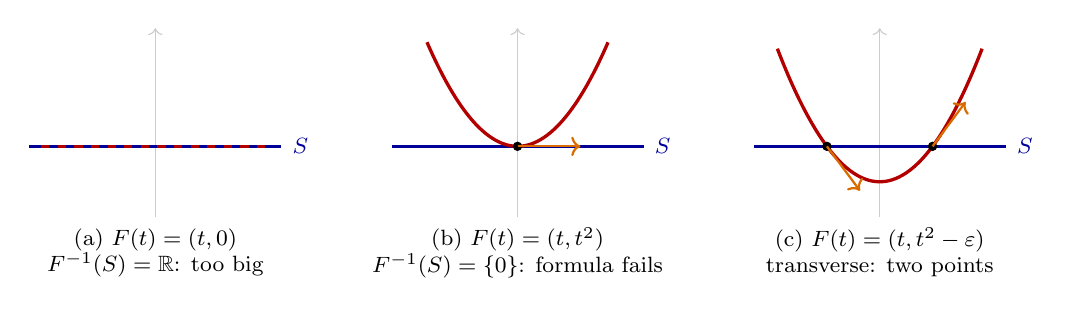
\begin{tikzpicture}[scale=1.0]
% ---- (a) curve lying in S
\draw[gray!40,->] (0,-0.9) -- (0,1.5);
\draw[blue!60!black,very thick] (-1.6,0) -- (1.6,0);
\draw[red!70!black,very thick,dashed] (-1.45,0) -- (1.45,0);
\node[blue!60!black,font=\footnotesize,anchor=west] at (1.62,0) {$S$};
\node[font=\footnotesize,align=center] at (0,-1.35) {(a) $F(t) = (t,0)$\\ $F^{-1}(S) = \mathbb{R}$: too big};
% ---- (b) tangent parabola
\begin{scope}[xshift=4.6cm]
\draw[gray!40,->] (0,-0.9) -- (0,1.5);
\draw[blue!60!black,very thick] (-1.6,0) -- (1.6,0);
\draw[red!70!black,very thick,domain=-1.15:1.15,samples=60,smooth,variable=\t] plot (\t,{\t*\t});
\fill[black] (0,0) circle (1.7pt);
\draw[orange!85!black,->,thick] (0,0) -- (0.8,0);
\node[blue!60!black,font=\footnotesize,anchor=west] at (1.62,0) {$S$};
\node[font=\footnotesize,align=center] at (0,-1.35) {(b) $F(t) = (t,t^2)$\\ $F^{-1}(S) = \{0\}$: formula fails};
\end{scope}
% ---- (c) perturbed, transverse
\begin{scope}[xshift=9.2cm]
\draw[gray!40,->] (0,-0.9) -- (0,1.5);
\draw[blue!60!black,very thick] (-1.6,0) -- (1.6,0);
\draw[red!70!black,very thick,domain=-1.3:1.3,samples=60,smooth,variable=\t] plot (\t,{\t*\t-0.45});
\fill[black] ({sqrt(0.45)},0) circle (1.7pt);
\fill[black] ({-sqrt(0.45)},0) circle (1.7pt);
\draw[orange!85!black,->,thick] ({sqrt(0.45)},0) -- ({sqrt(0.45)+0.42},{2*sqrt(0.45)*0.42});
\draw[orange!85!black,->,thick] ({-sqrt(0.45)},0) -- ({-sqrt(0.45)+0.42},{-2*sqrt(0.45)*0.42});
\node[blue!60!black,font=\footnotesize,anchor=west] at (1.62,0) {$S$};
\node[font=\footnotesize,align=center] at (0,-1.35) {(c) $F(t) = (t,t^2-\varepsilon)$\\ transverse: two points};
\end{scope}
\end{tikzpicture}
\end{center}

\begin{rembox}\label{rem:tangent-8}
Transversality protects the dimension and the tangent formula \emph{independently}: (a) loses the first, (b) keeps the first and loses the second. And (c) shows what happens to the tangency of (b) under an arbitrarily small perturbation: it disappears, replaced by two transverse crossings (for $\varepsilon > 0$) or by no intersection at all (for $\varepsilon < 0$). The same happens to the tangent plane of Example~\ref{ex:sphere-plane-transverse} when it is moved slightly up or down.
\end{rembox}

\begin{rembox}[Looking Ahead: Transversality Is Generic]\label{rem:looking-ahead-transversality-generic}
Two points of the remark above will be taken up once abstract manifolds and submanifolds are in place. First, the definition makes sense verbatim for a smooth map $F : X \to Y$ between abstract manifolds and a submanifold $S \subseteq Y$, with \emph{abstract} tangent spaces and the differential of \S\ref{sub:pushforward} in place of $T^{\geo}$ and the Jacobian:
\[
dF_p(T_pX) + T_{F(p)}S = T_{F(p)}Y \qquad \text{for all } p \in F^{-1}(S),
\]
and Theorem~\ref{thm:transverse-preimage} becomes the statement that \emph{the preimage of a submanifold under a transverse map is a submanifold of the same codimension}. Second, as Example~\ref{ex:transverse-failures}(c) suggests, transversality is the \emph{typical} situation: any smooth map can be made transverse to a given submanifold by an arbitrarily small perturbation, and tangencies are non-generic accidents. This is the transversality theorem of Thom, and it is the entry point to intersection theory (Guillemin--Pollack, Ch.~2). Neither is part of the course yet.
\end{rembox}

\begin{rembox}[What Is Still Missing]\label{rem:what-still-missing}
Everything above presupposes an ambient $\mathbb{R}^{n+k}$: Definition~\ref{def:geometric-tangent} of the geometric tangent space $T^{\geo}_pM$ uses its vector space structure to differentiate $\gamma$, and Theorem~\ref{thm:tangent-kernel} uses the Jacobian of the defining map $F$. For an abstract smooth manifold neither is available --- ``if you have a sphere you can think of the tangent plane, but that is a subspace of $\mathbb{R}^3$. If you do not have $\mathbb{R}^3$, then what do you do? You do not have room to put your vectors.'' The next sections build the \emph{abstract} tangent space $T_pM$ from the charts alone.
\end{rembox}

\section{Germs}\label{sub:germs}\label{sec:abstract-tangent}

\roadmark{Stage: abstract}{Germs of smooth functions at a point --- the objects that derivations act on, available on every manifold, including those built by quotients. The motivation from geometric tangent vectors closes \ref{sec:tangent}.}

Point (1) of Proposition~\ref{prop:Dv-properties}, at the end of \ref{sec:tangent}, is made official here: the objects a derivation eats are not functions but germs.

\begin{defbox}[Agreement Near a Point]\deflabel{def:germ-relation}
Let $M$ be a smooth manifold and $p \in M$. Consider pairs $(f, U)$ with $U \subseteq M$ open, $p \in U$, and $f : U \to \mathbb{R}$ smooth. Two such pairs \textbf{agree near $p$}, written $(f,U) \sim (g,V)$, if
\[
\text{there is an open } W \text{ with } p \in W \subseteq U \cap V \text{ and } f|_W = g|_W .
\]
\end{defbox}

\begin{propbox}[Agreement Near a Point Is an Equivalence Relation]\thmlabel{prop:germ-equivalence}
\begin{enumerate}
    \item $\sim$ is an equivalence relation.
    \item Finitely many pairs in one equivalence class agree on a common open neighbourhood of $p$.
\end{enumerate}
\end{propbox}

\begin{proof}
(1) \emph{Reflexive:} take $W = U$. \emph{Symmetric:} the condition is symmetric in the two pairs. \emph{Transitive:} if $f = g$ on an open $W_1 \ni p$ and $g = h$ on an open $W_2 \ni p$, then $f = h$ on $W_1 \cap W_2$, which is open, contains $p$, and lies in both domains.

(2) If $(f_1,U_1), \ldots, (f_k,U_k)$ are equivalent, then for each $i$ there is an open $W_i \ni p$ on which $f_1 = f_i$. On $W = W_2 \cap \cdots \cap W_k$, which is open and contains $p$, all the $f_i$ equal $f_1$. Both parts use only that a \emph{finite} intersection of open sets is open.
\end{proof}

\begin{defbox}[Germs of Smooth Functions]\deflabel{def:germ}
An equivalence class $[f]$ of the relation $\sim$ of Definition~\ref{def:germ-relation} is a \textbf{(}$C^\infty$\textbf{) germ at $p$}, and each pair $(f,U)$ in it is a \textbf{representative} of the germ. The set of all germs at $p$ is denoted $C_p^\infty(M)$.
\leeref{no counterpart; the course's germ-based route (Lee uses $C^\infty(M)$; see Proposition~\ref{prop:germ-global})}
\end{defbox}

\begin{center}
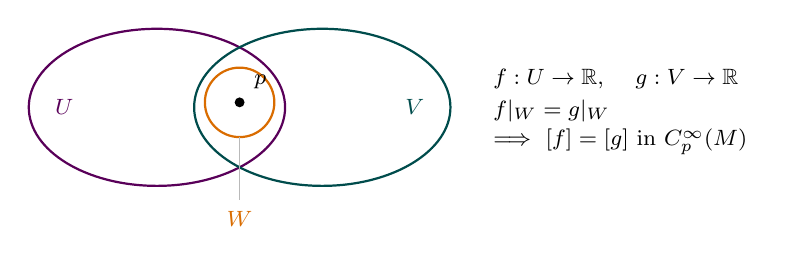
\begin{tikzpicture}[scale=1.05]
\draw[violet!70!black, thick] (0,0) ellipse (1.55 and 0.95);
\draw[teal!60!black, thick] (2.0,0) ellipse (1.55 and 0.95);
\node[violet!70!black,font=\footnotesize] at (-1.12,0) {$U$};
\node[teal!60!black,font=\footnotesize] at (3.12,0) {$V$};
\draw[orange!85!black, thick] (1.0,0.06) circle (0.42);
\draw[gray!55,thin] (1.0,-0.36) -- (1.0,-1.12);
\node[orange!85!black,font=\footnotesize,anchor=north] at (1.0,-1.14) {$W$};
\fill (1.0,0.06) circle (1.7pt);
\node[font=\footnotesize,anchor=south west] at (1.06,0.10) {$p$};
\node[font=\footnotesize,anchor=west] at (3.95,0.34) {$f : U \to \mathbb{R}$, \quad $g : V \to \mathbb{R}$};
\node[font=\footnotesize,anchor=west] at (3.95,-0.04) {$f|_W = g|_W$};
\node[font=\footnotesize,anchor=west] at (3.95,-0.42) {$\Longrightarrow\ [f] = [g]$ in $C_p^\infty(M)$};
\end{tikzpicture}
\end{center}

\begin{exbox}[No Neighbourhood Serves a Whole Germ]\exlabel{ex:germ-no-common-nbhd}
Part (2) of Proposition~\ref{prop:germ-equivalence} fails for infinitely many representatives. Work at $p = 0 \in \mathbb{R}$. Let $h(s) = e^{-1/s}$ for $s > 0$ and $h(s) = 0$ for $s \le 0$, the smooth flat function (see Example~\ref{ex:taylor-germs} below), and put
\[
f_n(x) = h\big(x^2 - 1/n^2\big), \qquad n = 1, 2, 3, \ldots
\]
Each $f_n$ is smooth on all of $\mathbb{R}$ and vanishes exactly on $[-1/n, 1/n]$, so $(f_n, \mathbb{R}) \sim (0, \mathbb{R})$: every $f_n$ represents the zero germ. Yet the set on which all of them agree with $0$ is $\bigcap_n [-1/n, 1/n] = \{0\}$, which contains no open neighbourhood of $0$. The same happens, even more simply, with the representatives $\big(0, (-1/n, 1/n)\big)$: no open set around $0$ lies in all of their domains.
\end{exbox}

\begin{rembox}\label{rem:abstract-tangent-2}
Nothing in the theory needs a common neighbourhood for a whole class. Every construction on germs --- sums, products and evaluation (Proposition~\ref{prop:germ-algebra}), derivations, pullbacks --- handles finitely many representatives at a time, and part (2) supplies the common neighbourhood for those. The obstruction in the example is exactly that an \emph{infinite} intersection of open sets need not be open. This is also the precise sense in which a germ is not a function on any particular neighbourhood of $p$: its representatives can be shrunk at will, but there is no smallest domain to shrink them to.
\end{rembox}

\begin{propbox}[$C_p^\infty(M)$ Is an $\mathbb{R}$-Algebra]\thmlabel{prop:germ-algebra}
The operations
\[
[f] + [g] = [f|_W + g|_W], \qquad [f]\,[g] = [f|_W \cdot g|_W], \qquad \lambda[f] = [\lambda f],
\]
where $W$ is any open set with $p \in W \subseteq U \cap V$, are well defined and make $C_p^\infty(M)$ a commutative ring with unit $[1]$ and an $\mathbb{R}$-vector space --- that is, a commutative $\mathbb{R}$-algebra. Moreover the evaluation map
\[
[f] \longmapsto [f](p) := f(p)
\]
is a well-defined $\mathbb{R}$-algebra homomorphism $C_p^\infty(M) \to \mathbb{R}$.
\leeref{no counterpart; the course's germ-based route}
\end{propbox}

\begin{proof}
\textit{(Lecture~8 sketched the operations --- ``taking representatives \ldots\ and shrinking to a common domain'' --- and skipped the checks as ``tedious''; they are filled in here.)} \emph{Existence of $W$ and smoothness.} $U \cap V$ is open and contains $p$, so $W = U \cap V$ will do; $f|_W + g|_W$ and $f|_W\, g|_W$ are smooth on $W$, so they define germs.

\emph{Independence of representatives.} Suppose $(f,U) \sim (f', U')$ and $(g,V) \sim (g',V')$, say $f = f'$ on $W_1 \ni p$ and $g = g'$ on $W_2 \ni p$. On the open set $W_1 \cap W_2 \ni p$ the four functions satisfy $f + g = f' + g'$ and $fg = f'g'$ pointwise, so the resulting germs agree. Independence of the auxiliary $W$ is the same argument with $f = f'$, $g = g'$.

\emph{Algebra axioms.} Each is an identity between germs that holds for representatives on a common domain, hence holds after passing to classes.

\emph{Evaluation.} If $(f,U) \sim (g,V)$ then $f = g$ near $p$, in particular $f(p) = g(p)$; and evaluation of functions is compatible with sums and products.
\end{proof}

\begin{defbox}[Evaluation of a Germ]\deflabel{def:germ-evaluation}
The \textbf{value} of a germ $[f] \in C_p^\infty(M)$ at $p$ is $[f](p) := f(p)$, independent of the representative by Proposition~\ref{prop:germ-algebra}. The map $C_p^\infty(M) \to \mathbb{R}$, $[f] \mapsto [f](p)$, is \textbf{evaluation} at $p$.
\end{defbox}

\begin{rembox}[How to Think About a Germ]\label{rem:how-think-about-germ}
Uribe: ``when I think of a germ, I think of a representative --- a smooth function defined in a neighbourhood --- but I know that it is a germ, which means I can shrink its domain arbitrarily, as long as I shrink it to a neighbourhood of $p$.'' In practice one works with representatives and checks at the end that the answer is unchanged by shrinking. The formal content of the definition is exactly that shrinking is free.
\end{rembox}

\begin{exbox}[Germs Versus Taylor Series]\exlabel{ex:taylor-germs}
Take $M = \mathbb{R}^n$ and $x_0 \in \mathbb{R}^n$. All partial derivatives of a function at $x_0$ depend only on its germ, so the Taylor series construction descends to a map into the ring of formal power series,
\[
\mathcal{T} : C_{x_0}^\infty(\mathbb{R}^n) \longrightarrow \mathbb{R}[[x^1, \ldots, x^n]], \qquad
\mathcal{T}[f] = \sum_{\alpha} \frac{1}{\alpha!}\, \frac{\partial^{|\alpha|} f}{\partial x^\alpha}(x_0)\, (x - x_0)^\alpha ,
\]
an $\mathbb{R}$-algebra homomorphism. It is \emph{surjective} but \emph{not injective}.
\end{exbox}

\begin{proof}[Justification]
Surjectivity is \textbf{Borel's theorem}: every formal power series is the Taylor series at $x_0$ of some smooth function. It is cited, not proved --- Uribe: ``that's not so easy to show, but it's true.'' Failure of injectivity is elementary. Uribe: ``You can have totally flat functions that are not zero''; the example is filled in. The function
\[
f(x) = \begin{cases} e^{-1/|x-x_0|^2}, & x \neq x_0,\\ 0, & x = x_0,\end{cases}
\]
is smooth with all partial derivatives vanishing at $x_0$ (a standard computation, not reproduced here), so $\mathcal{T}[f] = 0$ while $[f] \neq 0$.
\end{proof}

\begin{defbox}[Flat Germ]\deflabel{def:flat-germ}
A germ $[f] \in C_{x_0}^\infty(\mathbb{R}^n)$ is \textbf{flat} if all partial derivatives of $f$, of all orders, vanish at $x_0$; equivalently, $\mathcal{T}[f] = 0$. So the kernel of $\mathcal{T}$ consists exactly of the flat germs.
\end{defbox}

\begin{rembox}\label{rem:abstract-tangent-3}
The moral is that a germ carries strictly more information than its Taylor series --- ``one of the beauties of being in the $C^\infty$ category.'' This is the same phenomenon as the rigidity of $C^\omega$ noted after Definition~\ref{def:regularity-classes}: a real-analytic germ \emph{is} its Taylor series, which is why there are no analytic bump functions, whereas a $C^\infty$ germ has room to spare.
\end{rembox}

% ============================================================================
% SECTION: DERIVATIONS AND THE ABSTRACT TANGENT SPACE
% ============================================================================

\section{Derivations and the Abstract Tangent Space}\label{sec:derivations}\label{sub:derivations}

\roadmark{Stage: abstract}{The abstract tangent space $T_pM$ as the derivations at $p$, and the differential $F_{*p}$ that pushes them forward. The two notions of tangent space agree wherever both exist (Theorem~\ref{thm:ambient-abstract}).}

\begin{rembox}[Two Faces of a Tangent Vector]\label{rem:two-faces-tangent-vector}
Lecture 9 opened with a framing that the rest of the course keeps returning to. A tangent vector has two faces --- ``like Janus.'' It is a \emph{velocity}, the $\gamma'(0)$ of a curve --- an element of the geometric tangent space $T^{\geo}_pM$, which is how \S\ref{sub:derivations-motivation} met it; and it is a \emph{derivation}, an operator that eats germs and returns numbers --- an element of the abstract tangent space $T_pM$, the formal definition below. Formally they are different objects, and the relation between them has to be proved (Theorem~\ref{thm:ambient-abstract}). The same split will reappear for vector fields: as velocities attached to every point they \emph{generate dynamics}, and as operators they lead to the \emph{Lie derivative}.
\end{rembox}

\begin{defbox}[Derivation at a Point]\deflabel{def:derivation}
Let $M$ be a smooth manifold and $p \in M$. A \textbf{derivation at $p$} is an $\mathbb{R}$-linear map
\[
D : C_p^\infty(M) \longrightarrow \mathbb{R}
\]
satisfying the \textbf{Leibniz rule}
\[
D\big([f][g]\big) \;=\; f(p)\, D[g] \;+\; g(p)\, D[f] \qquad \text{for all } [f], [g] \in C_p^\infty(M),
\]
where $f(p) = [f](p)$ is the evaluation of Proposition~\ref{prop:germ-algebra}.
\leeref{Ch.~3, \emph{Tangent Vectors}, on $C^\infty(M)$ rather than germs}
\end{defbox}

\begin{defbox}[The Abstract Tangent Space]\deflabel{def:abstract-tangent}
The \textbf{(abstract) tangent space} to $M$ at $p$ is
\[
T_pM \;=\; \{\, \text{all derivations at } p \,\},
\]
a real vector space under the pointwise operations $(D + D')[f] = D[f] + D'[f]$ and $(\lambda D)[f] = \lambda\, D[f]$. An element $D \in T_pM$ is a \textbf{tangent vector} at $p$. It is not an arrow in any ambient space but a function on germs, $D : C^\infty_p(M) \to \mathbb{R}$, so $D[f]$ is a real number for each germ $[f]$ at $p$.
\leeref{Ch.~3, \emph{Tangent Vectors}, via $C^\infty(M)$ (see Proposition~\ref{prop:germ-global})}
\end{defbox}

\begin{proof}[Verification that $T_pM$ is a vector space]
$D + D'$ and $\lambda D$ are linear, being pointwise combinations of linear maps, and each satisfies the Leibniz rule because the rule is linear in $D$: for instance
\[
(D+D')([f][g]) = f(p)D[g] + g(p)D[f] + f(p)D'[g] + g(p)D'[f] = f(p)(D+D')[g] + g(p)(D+D')[f].
\]
The zero map is a derivation, and the vector space axioms hold pointwise.
\end{proof}

\begin{defbox}[The Ideal of Germs Vanishing at a Point]\deflabel{def:Ip}
The \textbf{ideal of germs vanishing at $p$} is
\[
I_p = \{\, [f] \in C_p^\infty(M) \mid f(p) = 0 \,\},
\]
the kernel of evaluation at $p$ (Definition~\ref{def:germ-evaluation}). Its \textbf{square} $I_p^2$ is the set of all finite sums $\sum_k [u_k][w_k]$ of products of two elements of $I_p$, the empty sum $0$ included.
\leeref{Problem 11-4, where $I_p \subseteq C^\infty(M)$ consists of global functions}
\end{defbox}

\begin{lembox}[$I_p$ and $I_p^2$]\thmlabel{lem:Ip-subspaces}
$I_p$ is an ideal of $C_p^\infty(M)$ and $I_p^2 \subseteq I_p$; both are linear subspaces.
\end{lembox}

\begin{proof}
$I_p$ is the kernel of the algebra homomorphism of evaluation (Proposition~\ref{prop:germ-algebra}), hence a linear subspace and an ideal: $[g][f] \in I_p$ whenever $[f] \in I_p$, since $g(p)f(p) = 0$. $I_p^2$ is closed under sums by construction and under scalars since $c\,[u][w] = [cu][w]$ with $[cu] \in I_p$; and each product $[u][w]$ lies in $I_p$, since $u(p)w(p) = 0$.
\end{proof}

\begin{lembox}[First Properties of Derivations]\thmlabel{lem:derivation-properties}
Let $D$ be a derivation at $p$, and $I_p$, $I_p^2$ as in Definition~\ref{def:Ip}.
\begin{enumerate}
    \item $D$ annihilates constants: if $c \in \mathbb{R}$ and $\underline{c}$ denotes the germ of the constant function $c$, then $D[\underline{c}] = 0$. Consequently $D[f] = D\big[f - \underline{f(p)}\big]$, so $D$ is determined by its values on $I_p$.
    \item $D$ annihilates products of vanishing germs: if $[f], [g] \in I_p$, then $D([f][g]) = 0$. Consequently $D$ vanishes on all of $I_p^2$.
\end{enumerate}
\leeref{Lemmas 3.1 and 3.4}
\end{lembox}

\begin{proof}
(1) The germ of the constant $1$ satisfies $[\underline 1] = [\underline 1][\underline 1]$, so by the Leibniz rule
\[
D[\underline 1] = D\big([\underline 1][\underline 1]\big) = 1 \cdot D[\underline 1] + 1 \cdot D[\underline 1] = 2\, D[\underline 1],
\]
whence $D[\underline 1] = 0$. For general $c$, linearity gives $D[\underline c] = c\, D[\underline 1] = 0$.

(2) Immediate from the Leibniz rule: $D([f][g]) = f(p)D[g] + g(p)D[f] = 0 + 0 = 0$. A general element of $I_p^2$ is a finite sum of such products, and $D$ is linear.
\end{proof}

Both parts were set as an exercise in Lecture 9, where Uribe noted that (2) is ``a very simple consequence of the product rule'' and is part of a problem on Assignment~3, which introduces the ideal $I_p$ under that name. In commutative algebra the same ideal is written $\mathfrak{m}_p$, the notation used in the remark at the end of \S\ref{sub:coordinate-derivations}.

\begin{rembox}\label{rem:abstract-tangent-4}
Uribe listed exactly these two as what must be shown before the basis theorem, and deferred them to the following lecture. They are the entire reason the Taylor--Hadamard expansion collapses: the constant term dies by (1), the quadratic remainder dies by (2), and only the linear term survives.
\end{rembox}

\begin{propbox}[Germ Derivations and Global Derivations]\thmlabel{prop:germ-global}
Lee defines $T_pM$ as the space of derivations of $C^\infty(M)$ at $p$: linear maps $v : C^\infty(M) \to \mathbb{R}$ with $v(fg) = f(p)\,vg + g(p)\,vf$. For $D \in T_pM$ in the sense of Definition~\ref{def:abstract-tangent}, the formula $v_D(f) = D[f]$ defines such a derivation, and $D \mapsto v_D$ is a linear isomorphism between the two spaces.
\leeref{Ch.~3, with Propositions 2.25 and 3.8}
\end{propbox}

\begin{proof}[Proof, granting smooth bump functions]
Taking germs is an algebra homomorphism $C^\infty(M) \to C_p^\infty(M)$ compatible with evaluation at $p$, so $v_D$ is a derivation, and $D \mapsto v_D$ is linear. Both remaining steps use a \emph{bump function}: for an open $U \ni p$, a smooth $\psi : M \to [0,1]$ supported in $U$ with $\psi \equiv 1$ near $p$ (Lee, Proposition 2.25; these notes do not construct one). \emph{Injective:} every germ $[f]$, with $f$ defined on $U$, has the global representative $\psi f$, extended by zero; so if $v_D = 0$ then $D[f] = v_D(\psi f) = 0$ for every germ. \emph{Surjective:} given Lee's $v$, set $D[f] = v(\tilde f)$ for any global $\tilde f$ representing $[f]$. This is well defined because $v$ is local --- if $\tilde f = \tilde g$ near $p$ then $v\tilde f = v\tilde g$ (Lee, Proposition 3.8, whose proof uses a bump function) --- it is a derivation on germs, and $v_D = v$.
\end{proof}

\textbf{Comparison with Lee.} This is where the course's algebraic route and Lee's part company. Lee works with global functions and pays for locality with bump functions: Proposition~3.8 shows a derivation of $C^\infty(M)$ only sees a function near $p$, and Proposition~3.9 identifies $T_pU$ with $T_pM$. Germs build locality into the definition, so the course needs no bump functions at all --- Lemma~\ref{lem:germs-local} is pure algebra. The proposition above is the bridge. Since the two spaces are isomorphic, every result about $T_pM$ in these notes transfers to Lee's, and conversely.


\subsection{Pushing Derivations Forward}\label{sub:pushforward}

\textit{Lecture 9. Derivations can be pushed forward along smooth maps. In lecture this appeared in the middle of the proof of the basis theorem, as a ``new derivation'' $\tilde D$ on $\mathbb{R}^n$ built from one on $M$, and was defined properly only afterwards --- ``the order of my presentation is not ideal.'' Here it comes first, so the proof can cite it.}

Throughout, $F : M \to N$ is a smooth map of smooth manifolds and $p \in M$. The construction has two steps: functions are pulled back, and derivations, being linear functionals on functions, are pushed forward by duality.

\begin{defbox}[Pullback of Germs]\deflabel{def:germ-pullback}
Let $F : M \to N$ be a smooth map between smooth manifolds, and $p \in M$, so that $F(p)$ is a point of $N$. Let $[g] \in C^\infty_{F(p)}(N)$ be a germ \emph{at the point $F(p)$ of $N$}, with a representative $(g, V)$: $V \subseteq N$ is open with $F(p) \in V$, and $g : V \to \mathbb{R}$ is smooth. Then $F^{-1}(V)$ is an open neighbourhood of $p$ in $M$, and $g \circ F : F^{-1}(V) \to \mathbb{R}$ is smooth (Lemma~\ref{lem:composition-smooth}), so $(g \circ F, F^{-1}(V))$ represents a germ at $p$ on $M$. The \textbf{pullback} of germs along $F$ at $p$ is the map
\[
F_p^* : C^\infty_{F(p)}(N) \longrightarrow C^\infty_p(M), \qquad F_p^*[g] = [\,g \circ F\,],
\]
which takes a germ on $N$ at $F(p)$ to a germ on $M$ at $p$. It does not depend on the representative $(g, V)$ (Proposition~\ref{prop:pullback-properties}).
\leeref{no counterpart; the course's germ-based route}
\end{defbox}

\begin{propbox}[Properties of the Pullback]\thmlabel{prop:pullback-properties}
Let $F : M \to N$ be smooth and $p \in M$. The map $F_p^* : C^\infty_{F(p)}(N) \to C^\infty_p(M)$ is well defined, it is a homomorphism of $\mathbb{R}$-algebras, and it is compatible with evaluation: for every germ $[g] \in C^\infty_{F(p)}(N)$,
\[
\big(F_p^*[g]\big)(p) = g\big(F(p)\big).
\]
In particular $F_p^*$ maps the germs on $N$ vanishing at $F(p)$ to germs on $M$ vanishing at $p$: $F_p^*\big(I_{F(p)}\big) \subseteq I_p$.
\end{propbox}

\begin{proof}
\emph{Well defined.} For a representative $(g, V)$, the set $F^{-1}(V)$ is open and contains $p$ because $F$ is continuous, and $g \circ F$ is smooth there by Lemma~\ref{lem:composition-smooth}. If $(g, V)$ and $(g', V')$ represent the same germ at $F(p)$, then $g = g'$ on some open $W$ with $F(p) \in W \subseteq V \cap V'$; so $g \circ F = g' \circ F$ on the open set $F^{-1}(W) \ni p$, and the two pulled-back germs at $p$ are equal.

\emph{Algebra homomorphism.} Composition with $F$ respects the pointwise operations: $(g + h)\circ F = g \circ F + h \circ F$, $(gh) \circ F = (g\circ F)(h \circ F)$, $(\lambda g)\circ F = \lambda (g \circ F)$, and $1 \circ F = 1$.

\emph{Evaluation.} $(g \circ F)(p) = g(F(p))$ by definition of composition.
\end{proof}

\begin{defbox}[Pushforward --- the Differential]\deflabel{def:pushforward}
Let $F : M \to N$ be smooth and $p \in M$, and let $D \in T_pM$ be a tangent vector at $p$ --- that is, a derivation at $p$, a linear map $D : C^\infty_p(M) \to \mathbb{R}$ satisfying the Leibniz rule. The \textbf{pushforward} of $D$ along $F$ is the map
\[
F_{*p}D : C^\infty_{F(p)}(N) \longrightarrow \mathbb{R}, \qquad \big(F_{*p}D\big)[g] \;:=\; D\big(F_p^*[g]\big) = D[\,g \circ F\,],
\]
defined on germs $[g]$ at $F(p)$ on $N$: pull the germ back to $p$, then apply $D$. In one line, $F_{*p}D = D \circ F_p^*$. It is a derivation at $F(p)$, i.e.\ an element of $T_{F(p)}N$ (Proposition~\ref{prop:pushforward-derivation}). Letting $D$ vary gives the \textbf{pushforward}, or \textbf{differential}, of $F$ at $p$,
\[
F_{*p} : T_pM \longrightarrow T_{F(p)}N, \qquad D \longmapsto F_{*p}D,
\]
a map from tangent vectors at $p$ in $M$ to tangent vectors at $F(p)$ in $N$, also written $dF_p$. (Uribe: ``the awkward notation $F_{*p}$.'') So $F_{*p}$ acts on derivations; its value $F_{*p}D$ is again a derivation, which acts on germs at $F(p)$.
\leeref{Ch.~3, \emph{The Differential of a Smooth Map}}
\end{defbox}

\begin{center}
\begin{tikzcd}[row sep=3em, column sep=4em]
C^\infty_{F(p)}(N) \arrow[r, "F_p^*"] \arrow[dr, "F_{*p}D"'] & C^\infty_p(M) \arrow[d, "D"] \\
& \mathbb{R}
\end{tikzcd}
\\[1.4em]
\begin{tikzcd}[row sep=1.1em, column sep=3.6em]
M \arrow[r, "F"] & N & \text{points: forward} \\
C^\infty_p(M) & C^\infty_{F(p)}(N) \arrow[l, "F_p^*"'] & \text{germs: backward} \\
T_pM \arrow[r, "F_{*p}"] & T_{F(p)}N & \text{derivations: forward}
\end{tikzcd}
\end{center}

Above, the definition as a diagram: $F_{*p}D = D \circ F_p^*$, a derivation at $F(p)$ obtained by first pulling the germ back to $p$ and then applying $D$. Below, the directions. Points move forward along $F$; functions move backward, since a function on $N$ composed with $F$ is a function on $M$; and derivations, being dual to functions, reverse the arrow once more and move forward again.

\begin{propbox}[The Differential Is a Linear Map of Abstract Tangent Spaces]\thmlabel{prop:pushforward-derivation}
For every $D \in T_pM$, $F_{*p}D$ is a derivation at $F(p)$; and $F_{*p} : T_pM \to T_{F(p)}N$ is linear.
\leeref{Ch.~3, \emph{The Differential of a Smooth Map}}
\end{propbox}

\begin{proof}
$F_{*p}D = D \circ F_p^*$ is linear, as a composite of linear maps. For the Leibniz rule, let $[g],[h] \in C^\infty_{F(p)}(N)$. Then
\[
\begin{aligned}
\big(F_{*p}D\big)\big([g][h]\big)
&= D\big(F_p^*[g]\cdot F_p^*[h]\big) \\
&= \big(F_p^*[g]\big)(p)\, D\big(F_p^*[h]\big) + \big(F_p^*[h]\big)(p)\, D\big(F_p^*[g]\big) \\
&= g(F(p))\,\big(F_{*p}D\big)[h] + h(F(p))\,\big(F_{*p}D\big)[g],
\end{aligned}
\]
using, in turn, that $F_p^*$ is multiplicative, the Leibniz rule for $D$ at $p$, and compatibility with evaluation. So $F_{*p}D$ is a derivation at $F(p)$. Linearity in $D$ holds because $(D + \lambda D')\circ F_p^* = D \circ F_p^* + \lambda\, D' \circ F_p^*$.
\end{proof}

Every object of this section, with what it is and where it lives. The rows go in order of the diagram above: germs travel backwards, from $N$ to $M$, and derivations forwards, from $M$ to $N$.

\begin{center}
\renewcommand{\arraystretch}{1.25}
\begin{tabular}{>{\raggedright\arraybackslash}p{2.6cm} >{\raggedright\arraybackslash}p{7.8cm} >{\raggedright\arraybackslash}p{2.9cm}}
\toprule
\textbf{Object} & \textbf{What it is} & \textbf{Lives in} \\ \midrule
$F$ & a smooth map & $M \to N$ \\
$p$, \ $F(p)$ & a point of $M$, and its image, a point of $N$ & $M$, \ $N$ \\
$[f]$ & a germ at $p$: a class of smooth functions defined near $p$ in $M$ & $C^\infty_p(M)$ \\
$[g]$ & a germ at $F(p)$: a class of smooth functions defined near $F(p)$ in $N$ & $C^\infty_{F(p)}(N)$ \\
$F_p^*$ & pullback, an algebra homomorphism, $[g] \mapsto [g \circ F]$ & $C^\infty_{F(p)}(N) \to C^\infty_p(M)$ \\
$D$ & a tangent vector at $p$: a derivation, a linear map $C^\infty_p(M) \to \mathbb{R}$ & $T_pM$ \\
$F_{*p}$ & pushforward, a linear map, $D \mapsto D \circ F_p^*$ & $T_pM \to T_{F(p)}N$ \\
$F_{*p}D$ & a tangent vector at $F(p)$: a derivation, a linear map $C^\infty_{F(p)}(N) \to \mathbb{R}$ & $T_{F(p)}N$ \\
$(F_{*p}D)[g]$ & a real number, equal to $D[g \circ F]$ & $\mathbb{R}$ \\
\bottomrule
\end{tabular}
\end{center}

The board justified the derivation property with ``since $F_p^*$ is a ring morphism.'' That is one of the two facts used, and not quite enough on its own: the Leibniz rule \emph{at $F(p)$} needs the coefficients $g(F(p))$ and $h(F(p))$, and these appear only because pullback is compatible with evaluation, $(g \circ F)(p) = g(F(p))$ --- the third equality above. It is automatic here, but it is a separate property from multiplicativity, and it is the one that moves the base point from $p$ to $F(p)$.

\begin{thmbox}[The Chain Rule]\thmlabel{prop:pushforward-functorial}
If $F : M \to N$ and $G : N \to P$ are smooth and $p \in M$, then
\[
(G \circ F)_{*p} = G_{*F(p)} \circ F_{*p} : T_pM \to T_{G(F(p))}P, \qquad (\mathrm{id}_M)_{*p} = \mathrm{id}_{T_pM} .
\]
\leeref{Proposition 3.6(b)}
\end{thmbox}

\begin{proof}
\textit{(Lecture~10: ``the proof of the chain rule is one line'' --- pullbacks compose in the opposite order, because composition is associative. The dualization that follows was set as an exercise, ``use this to conclude the proof''; it is filled in.)} Pullback reverses composition: $(G\circ F)_p^* = F_p^* \circ G_{F(p)}^*$, since $g \circ (G \circ F) = (g \circ G) \circ F$. Hence for $D \in T_pM$ and a germ $[g]$ at $G(F(p))$,
\[
\big((G\circ F)_{*p}D\big)[g] = D\big(F_p^*\, G_{F(p)}^*[g]\big) = \big(F_{*p}D\big)\big(G_{F(p)}^*[g]\big) = \big(G_{*F(p)}\,F_{*p}D\big)[g].
\]
The identity pulls back every germ to itself, so it pushes every derivation to itself.
\end{proof}

\begin{center}
\begin{tikzcd}[row sep=3.2em, column sep=3.4em]
M \arrow[r, "F"] \arrow[rr, bend left=28, "G \circ F"] & N \arrow[r, "G"] & P \\
T_pM \arrow[r, "F_{*p}"'] \arrow[rr, bend right=28, "(G \circ F)_{*p}"'] & T_{F(p)}N \arrow[r, "G_{*F(p)}"'] & T_{G(F(p))}P
\end{tikzcd}
\end{center}

The upper row is the composite of maps; the lower row says its differential is the composite of the differentials. In coordinates (Corollary~\ref{cor:chain-rule-coords}) it becomes the multiplication of Jacobian matrices --- the chain rule of calculus, now as a statement about manifolds.

\textbf{Lecture 10.} Uribe stated this as the Chain Rule and proved the pullback identity $(G \circ F)_p^* = F_p^* \circ G_{F(p)}^*$ on the board --- ``see, you know that this is the right point of view when proofs become one line'' --- leaving the dualization as an exercise; the displayed computation above is that exercise. Pullbacks compose in the \emph{opposite} order, so pushforwards, being their duals, compose in the \emph{same} order as the maps. (The theorem appeared here, ahead of the lecture, because the two results below depend on it.)

\begin{corbox}[Diffeomorphisms Induce Isomorphisms]\thmlabel{lem:germs-diffeo}
If $\Phi : M \to N$ is a diffeomorphism, then $\Phi_{*p} : T_pM \to T_{\Phi(p)}N$ is a linear isomorphism, with inverse $(\Phi^{-1})_{*\Phi(p)}$.
\leeref{Proposition 3.6(d)}
\end{corbox}

\begin{proof}
Apply Proposition~\ref{prop:pushforward-functorial} to $\Phi^{-1} \circ \Phi = \mathrm{id}_M$ and $\Phi \circ \Phi^{-1} = \mathrm{id}_N$.
\end{proof}

\begin{lembox}[Open Subsets Have the Same Abstract Tangent Spaces]\thmlabel{lem:germs-local}
Let $U \subseteq M$ be open with $p \in U$, and $\iota : U \hookrightarrow M$ the inclusion. Then $\iota_p^* : C^\infty_p(M) \to C^\infty_p(U)$ is restriction of germs, an isomorphism of $\mathbb{R}$-algebras, and consequently $\iota_{*p} : T_pU \to T_pM$ is a linear isomorphism. We use it to identify $T_pU = T_pM$.
\leeref{Proposition 3.9}
\end{lembox}

\begin{proof}
Restriction is well defined and an algebra homomorphism by Proposition~\ref{prop:pullback-properties}. It is surjective because a germ at $p$ on $U$ has a representative defined on an open subset of $U$, which is open in $M$ and so already represents a germ on $M$; and injective because if $f|_U$ and $g|_U$ agree near $p$ then $f$ and $g$ agree near $p$. A derivation on one algebra corresponds to exactly one on the other by composing with this isomorphism, so $\iota_{*p}$ is a bijection; it is linear by Proposition~\ref{prop:pushforward-derivation}.
\end{proof}

\begin{propbox}[Charts Are Diffeomorphisms]\thmlabel{prop:chart-diffeo}
If $(U, \varphi)$ is a smooth chart of $M$, then $\varphi : U \to \varphi(U)$ is a diffeomorphism. Consequently, for every $p \in U$,
\[
T_pM \;=\; T_pU \xrightarrow[\ \cong\ ]{\ \varphi_{*p}\ } T_{\varphi(p)}\,\varphi(U)
\]
is a linear isomorphism of abstract tangent spaces.
\end{propbox}

\begin{proof}
In the charts $(U,\varphi)$ on $U$ and $(\varphi(U), \mathrm{id})$ on $\varphi(U)$, both $\varphi$ and $\varphi^{-1}$ have coordinate representation the identity, so both are smooth (Definition~\ref{def:smooth-map}). The isomorphism is then Lemma~\ref{lem:germs-local} followed by Corollary~\ref{lem:germs-diffeo}.
\end{proof}

\begin{rembox}[The Chart Pushforward]\label{rem:chart-pushforward}
This is the $\tilde D$ of the lecture: for $D \in T_pM$, $\tilde D = \varphi_{*p}D$ acts by $\tilde D[g] = D[g \circ \varphi]$, identifying tangent vectors on $M$ with derivations at a point of an open subset of $\mathbb{R}^n$. Everything about the abstract tangent space $T_pM$ can therefore be settled in $\mathbb{R}^n$, which is how the basis theorem is proved.
\end{rembox}

% ============================================================================
% SECTION: COORDINATE DERIVATIONS AND THE BASIS THEOREM
% ============================================================================

\section{Coordinate Derivations and the Basis Theorem}\label{sec:basis-theorem}\label{sub:coordinate-derivations}

\roadmark{Stage: abstract}{Charts give derivations $\partial/\partial x^i|_p$, and they form a basis of $T_pM$: $\dim T_pM = \dim M$. The proof needs Taylor's theorem with a smooth remainder.}

\begin{defbox}[Coordinate Functions of a Chart]\deflabel{def:coordinate-functions}
Let $M$ be a smooth $n$-manifold.
\begin{enumerate}
    \item The \textbf{standard coordinate functions} on $\mathbb{R}^n$ are the projections
    \[
    r^i : \mathbb{R}^n \to \mathbb{R}, \qquad r^i(a^1, \ldots, a^n) = a^i, \qquad i = 1, \ldots, n.
    \]
    \item For a smooth chart $(U, \varphi)$, the \textbf{coordinate functions of the chart}, or \textbf{local coordinates} on $U$, are
    \[
    x^i := r^i \circ \varphi : U \to \mathbb{R}, \qquad\text{so that}\qquad \varphi = (x^1, \ldots, x^n), \quad\text{i.e. } \varphi(q) = \big(x^1(q), \ldots, x^n(q)\big).
    \]
    \item For a function $f$ defined on $U$, its \textbf{coordinate representation} in the chart is $f_\varphi = f \circ \varphi^{-1} : \varphi(U) \to \mathbb{R}$, as in Definition~\ref{def:smooth-function}; thus $f = f_\varphi \circ \varphi$ on $U$. In particular $(x^i)_\varphi = r^i \circ \varphi \circ \varphi^{-1} = r^i$ on $\varphi(U)$.
\end{enumerate}
\leeref{Ch.~1, \emph{Coordinate Charts}}
\end{defbox}

\begin{rembox}\label{rem:abstract-tangent-5}
\textbf{A notational discipline.} Uribe stopped to insist on this. The $x^i$ live \emph{upstairs}, as functions on the manifold, and the $r^i$ \emph{downstairs}, as functions on $\mathbb{R}^n$; conflating them is the main source of confusion in what follows. The identity $(x^i)_\varphi = r^i$ is the bridge between the two rows: it says that the coordinate functions, written in their own chart, are the standard coordinates. It also shows that each $x^i$ is a smooth function on $U$, by Definition~\ref{def:smooth-function}, since $r^i$ is smooth.
\end{rembox}

\begin{center}
\begin{tikzcd}[row sep=3.0em, column sep=3.4em]
& U \arrow[dl, "f"'] \arrow[d, "\varphi"] \arrow[dr, "x^i"] & \\
\mathbb{R} & \varphi(U) \subseteq \mathbb{R}^n \arrow[l, "f_\varphi"] \arrow[r, "r^i"'] & \mathbb{R}
\end{tikzcd}
\end{center}

The board diagram for this section. Both triangles commute: the left one says $f = f_\varphi \circ \varphi$, which is what smoothness of $f$ means; the right one is the \emph{definition} $x^i = r^i \circ \varphi$ of the $i$-th coordinate function on $U$ (Definition~\ref{def:coordinate-functions}). Everything upstairs is expressed downstairs by composing with $\varphi$, and the derivation about to be defined does its differentiating entirely on the bottom row, where partial derivatives already make sense.

\begin{defbox}[Coordinate Derivations]\deflabel{def:coordinate-derivation}
Let $(U,\varphi)$ be a smooth chart with $p \in U$, with coordinate functions $x^1, \ldots, x^n$ (Definition~\ref{def:coordinate-functions}), and let $i \in \{1,\ldots,n\}$. Define $\dfrac{\partial}{\partial x^i}\Big|_p : C_p^\infty(M) \to \mathbb{R}$ by
\[
\frac{\partial}{\partial x^i}\Big|_p [f] \;:=\; \frac{\partial f_\varphi}{\partial r^i}\big(\varphi(p)\big),
\]
the ordinary $i$-th partial derivative at $\varphi(p)$ of the coordinate representation $f_\varphi = f \circ \varphi^{-1}$. For a function $f$ smooth near $p$ we also write
\[
\frac{\partial f}{\partial x^i}(p) \;:=\; \frac{\partial}{\partial x^i}\Big|_p [f] \;=\; \frac{\partial f_\varphi}{\partial r^i}\big(\varphi(p)\big),
\]
the \textbf{partial derivative} of $f$ with respect to the coordinate $x^i$. It is defined by going downstairs: there is no other way to differentiate a function on a manifold with respect to a coordinate.
\leeref{Ch.~3, \emph{Computations in Coordinates}}
\end{defbox}

\begin{propbox}[Coordinate Derivations Are Derivations]\thmlabel{prop:coord-is-derivation}
$\dfrac{\partial}{\partial x^i}\Big|_p$ is well defined on germs and is a derivation at $p$.
\end{propbox}

\begin{proof}
\textit{(Lecture~8: ``it's linear, and the product rule will be inherited from the product rule of the ordinary partial derivatives'' --- the \emph{Linear} and \emph{Leibniz} steps below. Well-definedness is filled in.)} \emph{Well defined.} If $(f,U_1) \sim (g,U_2)$, then $f = g$ on an open $W \ni p$, so $f_\varphi = g_\varphi$ on the open set $\varphi(W \cap U) \ni \varphi(p)$; partial derivatives at a point depend only on the function near that point, so the two values agree. (Shrinking the chart domain also changes nothing, for the same reason.)

\emph{Linear.} $(\lambda f + g)_\varphi = \lambda f_\varphi + g_\varphi$, and partial differentiation is linear.

\emph{Leibniz.} $(fg)_\varphi = f_\varphi\, g_\varphi$, so by the ordinary product rule at $\varphi(p)$,
\[
\frac{\partial (fg)_\varphi}{\partial r^i}(\varphi(p)) = f_\varphi(\varphi(p))\,\frac{\partial g_\varphi}{\partial r^i}(\varphi(p)) + g_\varphi(\varphi(p))\,\frac{\partial f_\varphi}{\partial r^i}(\varphi(p)),
\]
and $f_\varphi(\varphi(p)) = f(p)$, $g_\varphi(\varphi(p)) = g(p)$.
\end{proof}

The proof of the Basis Theorem below needs a form of Taylor expansion whose remainder is not an estimate but an exact, \emph{smooth} term --- ``a theorem from calculus'' that is not usually taught there. It is built in two steps: first order, then the first-order statement applied again.

\begin{lembox}[Hadamard's Lemma]\thmlabel{lem:hadamard}
Let $W \subseteq \mathbb{R}^n$ be open, $a = (a^1,\ldots,a^n) \in W$, $f : W \to \mathbb{R}$ smooth, and $B \subseteq W$ an open ball centred at $a$. Then there are smooth functions $f_1, \ldots, f_n$ on $B$ with
\[
f(r) = f(a) + \sum_{i=1}^n (r^i - a^i)\, f_i(r) \quad (r \in B), \qquad f_i(a) = \frac{\partial f}{\partial r^i}(a) .
\]
Explicitly, $f_i(r) = \displaystyle\int_0^1 \frac{\partial f}{\partial r^i}\big(a + t(r-a)\big)\, dt$.
\leeref{cf.\ Theorem C.15, used in the proof of Proposition 3.2}
\end{lembox}

\begin{proof}
\textit{(Lecture~9: ``the proof is delightfully simple.'')} Fix $r \in B$. The segment $t \mapsto a + t(r - a)$, $t \in [0,1]$, runs from $a$ to $r$ and stays in $B$, a ball being convex. By the fundamental theorem of calculus and the chain rule,
\[
f(r) - f(a) = \int_0^1 \frac{d}{dt} f\big(a + t(r-a)\big)\, dt = \int_0^1 \sum_{i=1}^n (r^i - a^i)\, \frac{\partial f}{\partial r^i}\big(a + t(r-a)\big)\, dt = \sum_{i=1}^n (r^i - a^i)\, f_i(r),
\]
the factors $r^i - a^i$ coming out of the integral because they do not depend on $t$. Each $f_i$ is smooth on $B$: the integrand is smooth in $(t, r)$ on $[0,1] \times B$, so differentiation under the integral sign is legitimate to every order. At $r = a$ the integrand is constant, and $f_i(a) = \partial f/\partial r^i(a)$.
\end{proof}

\textbf{Transcription note.} In Lecture~9 the path in the integral was first written with the wrong endpoints; a student corrected it to the convex combination $t(r - a) + a$, which runs from $a$ at $t = 0$ to $r$ at $t = 1$, as above.

Uribe called the proof ``delightfully simple.'' A student corrected the path on the board: it must be the segment $a + t(r - a)$, equal to $a$ at $t = 0$ and to $r$ at $t = 1$. Convexity of $B$ is what the proof uses --- ``everything is local,'' but the neighbourhood must contain the segment from $a$ to each of its points, which is why a ball (or any set star-shaped about $a$) is taken.

\begin{lembox}[Taylor--Hadamard]\thmlabel{lem:taylor-hadamard}
In the setting of Lemma~\ref{lem:hadamard}, there are smooth functions $f_{ij}$ on $B$, $1 \le i, j \le n$, with
\[
f(r) \;=\; f(a) \;+\; \sum_{i=1}^n (r^i - a^i)\, \frac{\partial f}{\partial r^i}(a) \;+\; \sum_{i,j=1}^n (r^i - a^i)(r^j - a^j)\, f_{ij}(r) \qquad (r \in B),
\]
and $f_{ij}(a) = \tfrac12\, \dfrac{\partial^2 f}{\partial r^i\,\partial r^j}(a)$. This is an identity, not an approximation.
\leeref{cf.\ Theorem C.15}
\end{lembox}

\begin{proof}
\textit{(Lecture~9, exactly: first order, then ``apply the claim to each $f_i$'' and substitute back. Uribe wrote the quadratic term with a factor $\tfrac12$ --- ``doesn't matter'' --- which the notes absorb into $f_{ij}$; the value of $f_{ij}(a)$ at the end is a completion, the lecture needing only that the $f_{ij}$ are smooth.)} Apply Lemma~\ref{lem:hadamard} to $f$, obtaining $f_1, \ldots, f_n$; then apply it again to each $f_i$, obtaining smooth $f_{ij}$ with
\[
f_i(r) = f_i(a) + \sum_{j=1}^n (r^j - a^j)\, f_{ij}(r) = \frac{\partial f}{\partial r^i}(a) + \sum_{j=1}^n (r^j - a^j)\, f_{ij}(r).
\]
Substituting this into $f(r) = f(a) + \sum_i (r^i - a^i) f_i(r)$ gives the identity. For the value at $a$: by Lemma~\ref{lem:hadamard} applied to $f_i$, $f_{ij}(a) = \partial f_i/\partial r^j(a)$, and differentiating the integral formula for $f_i$ under the integral sign,
\[
\frac{\partial f_i}{\partial r^j}(r) = \int_0^1 t\, \frac{\partial^2 f}{\partial r^j\,\partial r^i}\big(a + t(r-a)\big)\, dt, \qquad\text{so}\qquad \frac{\partial f_i}{\partial r^j}(a) = \frac12\, \frac{\partial^2 f}{\partial r^i\,\partial r^j}(a). \qedhere
\]
\end{proof}

\textbf{On the factor $\tfrac12$.} The board states the lemma with $\tfrac12 \sum_{i,j}$ in front of the quadratic term; Uribe added it ``just for consistency,'' saying it ``doesn't matter.'' For the \emph{existence} statement that is right --- replacing $f_{ij}$ by $2f_{ij}$ converts one form into the other. But the two forms are not interchangeable as written: the iterated proof above produces the version \emph{without} the $\tfrac12$, and with $f_{ij}(a) = \tfrac12 \partial_{ij} f(a)$. The board's normalization is the one in which $f_{ij}(a) = \partial_{ij} f(a)$, matching the Hessian term $\tfrac12 \sum \partial_{ij}f(a)(r^i - a^i)(r^j - a^j)$ of the ordinary Taylor polynomial. A numerical check on a test function confirms the unscaled identity to machine precision and shows the scaled one, with the same $f_{ij}$, to be off. Nothing below depends on the normalization, since only the vanishing of the quadratic term under a derivation is used.

\begin{rembox}\label{rem:abstract-tangent-6}
\textbf{What matters.} ``The point is that these functions don't blow up at $a$'': the remainder is a product of two factors vanishing at $a$ with a \emph{smooth} function, not merely a quantity that is small compared with $|r - a|^2$. The same iteration continues to any order.
\end{rembox}

\begin{center}
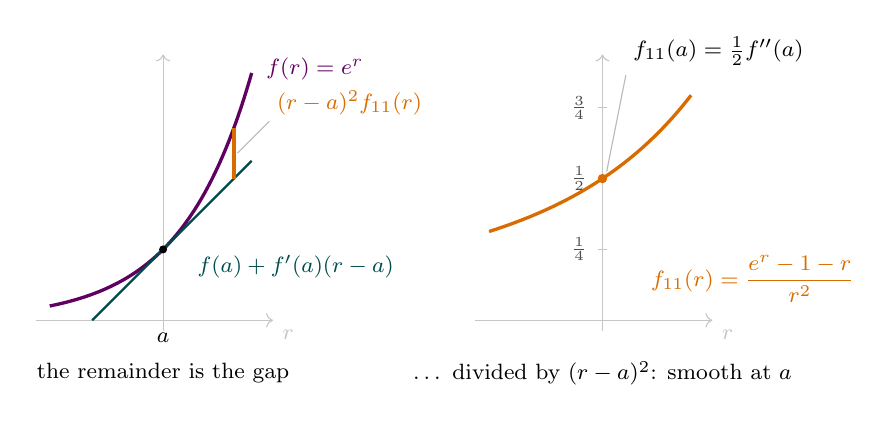
\begin{tikzpicture}[scale=0.9]
\draw[gray!45,->] (-1.8,0) -- (1.55,0) node[anchor=north west,font=\footnotesize]{$r$};
\draw[gray!45,->] (0,-0.15) -- (0,3.75);
\draw[violet!75!black,very thick] (-1.6000,0.2019) -- (-1.5795,0.2061) -- (-1.5590,0.2103) -- (-1.5385,0.2147) -- (-1.5180,0.2192) -- (-1.4975,0.2237) -- (-1.4770,0.2283) -- (-1.4565,0.2331) -- (-1.4360,0.2379) -- (-1.4155,0.2428) -- (-1.3950,0.2478) -- (-1.3745,0.2530) -- (-1.3540,0.2582) -- (-1.3335,0.2636) -- (-1.3129,0.2690) -- (-1.2924,0.2746) -- (-1.2719,0.2803) -- (-1.2514,0.2861) -- (-1.2309,0.2920) -- (-1.2104,0.2981) -- (-1.1899,0.3042) -- (-1.1694,0.3105) -- (-1.1489,0.3170) -- (-1.1284,0.3235) -- (-1.1079,0.3302) -- (-1.0874,0.3371) -- (-1.0669,0.3441) -- (-1.0464,0.3512) -- (-1.0259,0.3585) -- (-1.0054,0.3659) -- (-0.9849,0.3735) -- (-0.9644,0.3812) -- (-0.9439,0.3891) -- (-0.9234,0.3972) -- (-0.9029,0.4054) -- (-0.8824,0.4138) -- (-0.8619,0.4224) -- (-0.8414,0.4311) -- (-0.8209,0.4401) -- (-0.8004,0.4492) -- (-0.7799,0.4585) -- (-0.7594,0.4680) -- (-0.7388,0.4777) -- (-0.7183,0.4876) -- (-0.6978,0.4977) -- (-0.6773,0.5080) -- (-0.6568,0.5185) -- (-0.6363,0.5292) -- (-0.6158,0.5402) -- (-0.5953,0.5514) -- (-0.5748,0.5628) -- (-0.5543,0.5745) -- (-0.5338,0.5864) -- (-0.5133,0.5985) -- (-0.4928,0.6109) -- (-0.4723,0.6236) -- (-0.4518,0.6365) -- (-0.4313,0.6497) -- (-0.4108,0.6631) -- (-0.3903,0.6769) -- (-0.3698,0.6909) -- (-0.3493,0.7052) -- (-0.3288,0.7198) -- (-0.3083,0.7347) -- (-0.2878,0.7499) -- (-0.2673,0.7655) -- (-0.2468,0.7813) -- (-0.2263,0.7975) -- (-0.2058,0.8140) -- (-0.1853,0.8309) -- (-0.1647,0.8481) -- (-0.1442,0.8657) -- (-0.1237,0.8836) -- (-0.1032,0.9019) -- (-0.0827,0.9206) -- (-0.0622,0.9397) -- (-0.0417,0.9591) -- (-0.0212,0.9790) -- (-0.0007,0.9993) -- (0.0198,1.0200) -- (0.0403,1.0411) -- (0.0608,1.0627) -- (0.0813,1.0847) -- (0.1018,1.1072) -- (0.1223,1.1301) -- (0.1428,1.1535) -- (0.1633,1.1774) -- (0.1838,1.2018) -- (0.2043,1.2267) -- (0.2248,1.2521) -- (0.2453,1.2780) -- (0.2658,1.3045) -- (0.2863,1.3315) -- (0.3068,1.3591) -- (0.3273,1.3873) -- (0.3478,1.4160) -- (0.3683,1.4453) -- (0.3888,1.4753) -- (0.4094,1.5058) -- (0.4299,1.5370) -- (0.4504,1.5689) -- (0.4709,1.6014) -- (0.4914,1.6345) -- (0.5119,1.6684) -- (0.5324,1.7030) -- (0.5529,1.7382) -- (0.5734,1.7743) -- (0.5939,1.8110) -- (0.6144,1.8485) -- (0.6349,1.8868) -- (0.6554,1.9259) -- (0.6759,1.9658) -- (0.6964,2.0065) -- (0.7169,2.0481) -- (0.7374,2.0905) -- (0.7579,2.1338) -- (0.7784,2.1780) -- (0.7989,2.2231) -- (0.8194,2.2692) -- (0.8399,2.3162) -- (0.8604,2.3642) -- (0.8809,2.4132) -- (0.9014,2.4631) -- (0.9219,2.5142) -- (0.9424,2.5663) -- (0.9629,2.6194) -- (0.9835,2.6737) -- (1.0040,2.7291) -- (1.0245,2.7856) -- (1.0450,2.8433) -- (1.0655,2.9022) -- (1.0860,2.9623) -- (1.1065,3.0237) -- (1.1270,3.0863) -- (1.1475,3.1503) -- (1.1680,3.2155) -- (1.1885,3.2821) -- (1.2090,3.3501) -- (1.2295,3.4195) -- (1.2500,3.4903);
\draw[teal!60!black,thick] (-1.0000,0.0000) -- (1.2500,2.2500);
\fill (0,1) circle (1.6pt);
\draw[orange!85!black,very thick] (1.0,2.0000) -- (1.0,2.7183);
\draw[gray!55,thin] (1.05,2.3591) -- (1.5,2.8091);
\node[orange!85!black,font=\footnotesize,anchor=south west] at (1.47,2.7591) {$(r-a)^2 f_{11}(r)$};
\node[violet!75!black,font=\footnotesize,anchor=west] at (1.32,3.55) {$f(r)=e^r$};
\node[teal!60!black,font=\footnotesize,anchor=north west] at (0.35,1.05) {$f(a)+f'(a)(r-a)$};
\node[font=\footnotesize,anchor=north] at (0,-0.04) {$a$};
\node[font=\footnotesize,align=center] at (0,-0.75) {the remainder is the gap};
\begin{scope}[xshift=6.2cm]
\draw[gray!45,->] (-1.8,0) -- (1.55,0) node[anchor=north west,font=\footnotesize]{$r$};
\draw[gray!45,->] (0,-0.15) -- (0,3.75);
\draw[gray!45] (-0.07,1.0) -- (0.07,1.0); \node[gray!60!black,font=\scriptsize,anchor=east] at (-0.08,1.0) {$\tfrac14$};
\draw[gray!45] (-0.07,2.0) -- (0.07,2.0); \node[gray!60!black,font=\scriptsize,anchor=east] at (-0.08,2.0) {$\tfrac12$};
\draw[gray!45] (-0.07,3.0) -- (0.07,3.0); \node[gray!60!black,font=\scriptsize,anchor=east] at (-0.08,3.0) {$\tfrac34$};
\draw[orange!85!black,very thick] (-1.6000,1.2530) -- (-1.5795,1.2595) -- (-1.5590,1.2662) -- (-1.5385,1.2729) -- (-1.5180,1.2796) -- (-1.4975,1.2864) -- (-1.4770,1.2933) -- (-1.4565,1.3002) -- (-1.4360,1.3072) -- (-1.4155,1.3142) -- (-1.3950,1.3213) -- (-1.3745,1.3285) -- (-1.3540,1.3357) -- (-1.3335,1.3431) -- (-1.3129,1.3504) -- (-1.2924,1.3579) -- (-1.2719,1.3654) -- (-1.2514,1.3729) -- (-1.2309,1.3806) -- (-1.2104,1.3883) -- (-1.1899,1.3960) -- (-1.1694,1.4039) -- (-1.1489,1.4118) -- (-1.1284,1.4198) -- (-1.1079,1.4278) -- (-1.0874,1.4360) -- (-1.0669,1.4442) -- (-1.0464,1.4525) -- (-1.0259,1.4608) -- (-1.0054,1.4693) -- (-0.9849,1.4778) -- (-0.9644,1.4864) -- (-0.9439,1.4951) -- (-0.9234,1.5038) -- (-0.9029,1.5127) -- (-0.8824,1.5216) -- (-0.8619,1.5306) -- (-0.8414,1.5397) -- (-0.8209,1.5489) -- (-0.8004,1.5581) -- (-0.7799,1.5675) -- (-0.7594,1.5769) -- (-0.7388,1.5865) -- (-0.7183,1.5961) -- (-0.6978,1.6058) -- (-0.6773,1.6156) -- (-0.6568,1.6255) -- (-0.6363,1.6355) -- (-0.6158,1.6456) -- (-0.5953,1.6558) -- (-0.5748,1.6661) -- (-0.5543,1.6765) -- (-0.5338,1.6870) -- (-0.5133,1.6976) -- (-0.4928,1.7083) -- (-0.4723,1.7191) -- (-0.4518,1.7300) -- (-0.4313,1.7410) -- (-0.4108,1.7521) -- (-0.3903,1.7633) -- (-0.3698,1.7747) -- (-0.3493,1.7861) -- (-0.3288,1.7977) -- (-0.3083,1.8094) -- (-0.2878,1.8212) -- (-0.2673,1.8331) -- (-0.2468,1.8452) -- (-0.2263,1.8573) -- (-0.2058,1.8696) -- (-0.1853,1.8820) -- (-0.1647,1.8945) -- (-0.1442,1.9072) -- (-0.1237,1.9200) -- (-0.1032,1.9329) -- (-0.0827,1.9460) -- (-0.0622,1.9592) -- (-0.0417,1.9725) -- (-0.0212,1.9859) -- (-0.0007,1.9995) -- (0.0198,2.0133) -- (0.0403,2.0271) -- (0.0608,2.0412) -- (0.0813,2.0553) -- (0.1018,2.0696) -- (0.1223,2.0841) -- (0.1428,2.0987) -- (0.1633,2.1135) -- (0.1838,2.1284) -- (0.2043,2.1435) -- (0.2248,2.1587) -- (0.2453,2.1741) -- (0.2658,2.1897) -- (0.2863,2.2054) -- (0.3068,2.2213) -- (0.3273,2.2373) -- (0.3478,2.2535) -- (0.3683,2.2700) -- (0.3888,2.2865) -- (0.4094,2.3033) -- (0.4299,2.3202) -- (0.4504,2.3373) -- (0.4709,2.3546) -- (0.4914,2.3721) -- (0.5119,2.3898) -- (0.5324,2.4077) -- (0.5529,2.4257) -- (0.5734,2.4440) -- (0.5939,2.4624) -- (0.6144,2.4811) -- (0.6349,2.5000) -- (0.6554,2.5190) -- (0.6759,2.5383) -- (0.6964,2.5578) -- (0.7169,2.5775) -- (0.7374,2.5974) -- (0.7579,2.6176) -- (0.7784,2.6379) -- (0.7989,2.6585) -- (0.8194,2.6794) -- (0.8399,2.7004) -- (0.8604,2.7217) -- (0.8809,2.7432) -- (0.9014,2.7650) -- (0.9219,2.7870) -- (0.9424,2.8093) -- (0.9629,2.8318) -- (0.9835,2.8546) -- (1.0040,2.8776) -- (1.0245,2.9009) -- (1.0450,2.9244) -- (1.0655,2.9482) -- (1.0860,2.9723) -- (1.1065,2.9967) -- (1.1270,3.0213) -- (1.1475,3.0463) -- (1.1680,3.0715) -- (1.1885,3.0970) -- (1.2090,3.1228) -- (1.2295,3.1489) -- (1.2500,3.1753);
\fill[orange!85!black] (0,2.0) circle (1.9pt);
\draw[gray!55,thin] (0.06,2.1) -- (0.33,3.46);
\node[font=\footnotesize,anchor=south west] at (0.3,3.46) {$f_{11}(a)=\tfrac12 f''(a)$};
\node[orange!85!black,font=\footnotesize,anchor=north west] at (0.55,1.05) {$f_{11}(r)=\dfrac{e^r-1-r}{r^2}$};
\node[font=\footnotesize,align=center] at (0,-0.75) {\dots\ divided by $(r-a)^2$: smooth at $a$};
\end{scope}
\end{tikzpicture}
\end{center}

Taylor--Hadamard for $f(r) = e^r$ at $a = 0$, in one variable. Left: the remainder $f(r) - f(a) - f'(a)(r-a)$ is the gap between the graph and its tangent line. Right: the same gap divided by $(r - a)^2$. The quotient $f_{11}(r) = (e^r - 1 - r)/r^2$ has only a removable singularity at $a$: it is smooth there, with value $\tfrac12 = \tfrac12 f''(0)$, exactly as the lemma predicts, and as the iterated proof computes it --- $f_1(r) = (e^r - 1)/r$, then $f_{11}(r) = (f_1(r) - f_1(0))/r$. That the quotient extends smoothly across $a$ is the whole content of the lemma.

\begin{corbox}[Derivations on $\mathbb{R}^n$]\thmlabel{cor:derivations-Rn}
Let $W \subseteq \mathbb{R}^n$ be open, $a \in W$, and $D$ a derivation at $a$ on $W$. Then for every germ $[f]$ at $a$,
\[
D[f] = \sum_{i=1}^n \frac{\partial f}{\partial r^i}(a)\, D[r^i], \qquad\text{that is,}\qquad D = \sum_{i=1}^n D[r^i]\, \frac{\partial}{\partial r^i}\Big|_a .
\]
\leeref{Proposition 3.2 and Corollary 3.3}
\end{corbox}

\begin{proof}
Choose a representative $f$ on an open ball $B \subseteq W$ centred at $a$, which changes nothing since $D$ acts on germs, and apply $D$ to the identity of Lemma~\ref{lem:taylor-hadamard}:
\[
D[f] = D\big[\underline{f(a)}\big] + \sum_{i} \frac{\partial f}{\partial r^i}(a)\, D\big[r^i - a^i\big] + \sum_{i,j} D\Big[(r^i - a^i)\cdot\big((r^j - a^j) f_{ij}\big)\Big].
\]
The constant term vanishes by Lemma~\ref{lem:derivation-properties}(1). Each quadratic term is $D$ of a product of two germs in $I_a$ --- namely $r^i - a^i$ and $(r^j - a^j)f_{ij}$, both zero at $a$ --- so it vanishes by Lemma~\ref{lem:derivation-properties}(2). Finally $D[r^i - a^i] = D[r^i]$ by (1) again. So $D$ sees only the linear part of $f$: ``the ultimate formula in the Euclidean case.''
\end{proof}

\begin{thmbox}[Basis Theorem]\thmlabel{thm:tangent-basis}
Let $M$ be a smooth $n$-manifold, $p \in M$, and $(U, \varphi)$ any smooth chart with $p \in U$. Then
\[
\left\{ \frac{\partial}{\partial x^1}\Big|_p, \ \ldots, \ \frac{\partial}{\partial x^n}\Big|_p \right\}
\]
is a basis of $T_pM$; in particular $\dim T_pM = n$. Explicitly, every derivation $D$ at $p$ satisfies the \textbf{universal formula}
\[
D \;=\; \sum_{i=1}^n D\big[x^i\big]\, \frac{\partial}{\partial x^i}\Big|_p .
\]
\leeref{Proposition 3.15 and Corollary 3.3}
\end{thmbox}

\begin{proof}
\textit{(Lecture~9. In lecture the derivation $\tilde D$ was introduced inside this proof --- ``this is how you push forward derivations \ldots\ we'll come back to this construction immediately after'' --- and Uribe remarked that ``the order of my presentation is not ideal.'' The notes define the pushforward first, in \ref{sub:pushforward}, so that the proof can cite it.)} Let $D \in T_pM$ and put $a = \varphi(p) = (r_0^1, \ldots, r_0^n)$.

\emph{Step 1: push $D$ down.} Let $\tilde D = \varphi_{*p}D \in T_a\,\varphi(U)$, the chart pushforward of Proposition~\ref{prop:chart-diffeo}; so $\tilde D[g] = D[g \circ \varphi]$ for germs $g$ at $a$.

\emph{Step 2: apply the Euclidean formula downstairs.} By Corollary~\ref{cor:derivations-Rn} on the open set $\varphi(U)$,
\[
\tilde D[g] = \sum_{i=1}^n \frac{\partial g}{\partial r^i}(a)\, \tilde D[r^i] .
\]

\emph{Step 3: read it back upstairs.} Let $[f]$ be a germ at $p$, and take $g = f_\varphi = f \circ \varphi^{-1}$. Then $f_\varphi \circ \varphi = f$ near $p$, so $\tilde D[f_\varphi] = D[f]$; by Definition~\ref{def:coordinate-derivation}, $\partial f_\varphi/\partial r^i(a) = \partial/\partial x^i|_p[f]$; and $\tilde D[r^i] = D[r^i \circ \varphi] = D[x^i]$. Substituting,
\[
D[f] = \sum_{i=1}^n D[x^i]\, \frac{\partial}{\partial x^i}\Big|_p[f] \qquad\text{for every germ } [f],
\]
so $D = \sum_i D[x^i]\, \partial/\partial x^i|_p$ and the coordinate derivations span.

\emph{Step 4: independence.} If $\sum_i c_i\, \partial/\partial x^i|_p = 0$, apply it to $[x^j]$. Since $(x^j)_\varphi = r^j$, we get $\partial/\partial x^i|_p[x^j] = \partial r^j/\partial r^i = \delta^j_i$, hence $c_j = 0$. So the $n$ coordinate derivations form a basis, and the coefficients of $D$ are the numbers $D[x^i]$ --- uniquely.
\end{proof}

\begin{center}
\begin{tikzcd}[row sep=3.2em, column sep=4.4em]
C^\infty_{a}\big(\varphi(U)\big) \arrow[r, "\varphi^*"] \arrow[dr, "\tilde D \,=\, \varphi_{*p}D"'] & C^\infty_p(U) = C^\infty_p(M) \arrow[d, "D"] \\
& \mathbb{R}
\end{tikzcd}
\qquad
\begin{tabular}{c}
$\varphi^*[r^i] = [x^i]$ \\[3pt]
$\varphi^*[f_\varphi] = [f]$
\end{tabular}
\end{center}

The proof in one diagram --- the defining triangle of the pushforward, for the chart. Downstairs the Euclidean formula computes $\tilde D$ on everything; the two pullback identities on the right carry the answer back upstairs, turning $\tilde D[r^i]$ into $D[x^i]$ and $\tilde D[f_\varphi]$ into $D[f]$.

\textbf{Reconciliation with the lecture.} This is the lecture's proof, in the lecture's order of ideas but with the pushforward defined before it is used rather than after. Two details of the board version. It opens with ``$\forall\, [f] \in I_p$'': restricting to germs vanishing at $p$ is harmless, since $D[f] = D[f - f(p)]$ by Lemma~\ref{lem:derivation-properties}(1), but the argument works verbatim for every germ. And the notes had filled in a proof of this theorem before Lecture 9, via two reduction lemmas; those were the pushforward by an inclusion and by the chart in disguise, and they now appear as Lemma~\ref{lem:germs-local} and Corollary~\ref{lem:germs-diffeo}.

\textbf{Transcription note (Lecture 8).} Page 16 of the handwritten notes states Taylor--Hadamard for ``$f : U \to \mathbb{R}^2$''; the target is $\mathbb{R}$.

\begin{thmbox}[Ambient and Abstract Agree]\thmlabel{thm:ambient-abstract}
Let $M = F^{-1}(c) \subseteq \mathbb{R}^{n+k}$ be a regular level set and $p \in M$. Then
\[
T^{\geo}_pM \longrightarrow T_pM, \qquad v \longmapsto D_v,
\]
from the geometric tangent space (a subspace of $\mathbb{R}^{n+k}$) to the abstract tangent space (derivations at $p$) is an isomorphism of vector spaces.
\leeref{Propositions 3.2, 5.37 and 5.38}
\end{thmbox}

\begin{proof}[Proof]
\textbf{Announced in lecture.} Stated in lecture in answer to a student's question --- ``are the ambient and the abstract tangent spaces the same, just defined differently?'' --- with the answer that they are, but that it has to be proved. Injectivity is Proposition~\ref{prop:Dv-determines-v}; that $D_v$ really is a derivation is Proposition~\ref{prop:Dv-properties}; surjectivity follows from the basis theorem (Theorem~\ref{thm:tangent-basis}), both spaces having dimension $n$. Even once it is proved, the notes keep the notations apart: $T^{\geo}_pM$ is the geometric tangent space, $T_pM$ the abstract one.
\end{proof}
\begin{corbox}[Consequences]\thmlabel{cor:tangent-basis-consequences}
Let $M$ be a smooth $n$-manifold and $p \in M$. Then the abstract tangent space has $\dim T_pM = n$, and for a regular level set $M = F^{-1}(c)$ the map $v \mapsto D_v$ of Theorem~\ref{thm:ambient-abstract}, from $T^{\geo}_pM$ to $T_pM$, is an isomorphism.
\leeref{Proposition 3.10}
\end{corbox}

\begin{proof}
The first claim is Theorem~\ref{thm:tangent-basis}. For the second, $v \mapsto D_v$ is linear and injective (Proposition~\ref{prop:Dv-determines-v}) between spaces of dimension $n$ --- the geometric tangent space $T^{\geo}_pM$ by Theorem~\ref{thm:tangent-kernel}, the abstract tangent space $T_pM$ by Theorem~\ref{thm:tangent-basis} --- hence an isomorphism.
\end{proof}

\textbf{Comparison with Lee.} Lee meets the two kinds of tangent vector in the opposite order. He defines $T_pM$ by derivations first, identifies geometric and abstract tangent vectors in $\mathbb{R}^n$ (Proposition~3.2), and only later, for embedded submanifolds, shows $T_pS = \ker d\Phi_p$ (Proposition~5.38). The course starts geometrically, with $T^{\geo}_pM = \ker F'(p)$ inside the ambient space (Theorem~\ref{thm:tangent-kernel}), and reaches derivations afterwards. The consequence above is where the two orders meet.

\begin{rembox}[A Derivation Sees Only the First Derivatives]\label{rem:derivation-sees-only-first-derivatives}
The basis theorem showed that, of the whole Taylor expansion of a germ, a derivation sees only the \emph{linear} term --- ``of the entire Taylor series of the germ, all I care about are the first partials.'' \S\ref{sub:cotangent-germs} says this algebraically: $I_p$ is a maximal ideal, being the kernel of evaluation; $I_p^2$ consists exactly of the germs vanishing to \emph{second} order (Proposition~\ref{prop:second-order}); and $I_p/I_p^2$ is canonically the \emph{cotangent space} $T_p^*M$ of Definition~\ref{def:cotangent}, built with no dualizing at all (Theorem~\ref{thm:cotangent-ideal}). This is the sense in which, as Uribe remarked when he first set out to define the abstract tangent space, ``it is more natural to define the dual'': the cotangent space comes first, and the abstract tangent space is its dual. We follow Lee and do not take that route.
\end{rembox}

\begin{thmbox}[Dimension of the Tangent Space]\thmlabel{thm:tangent-dimension}
Let $M$ be a smooth $n$-manifold. Then for every $p \in M$,
\[
\dim T_pM = n = \dim M ,
\]
the same at every point, and independent of the chart used to compute it.
\end{thmbox}

\begin{proof}
\textit{(The last clause of the basis theorem, recorded as a theorem in its own right.)} Any chart $(U, \varphi)$ at $p$ has $n$ coordinate functions, and by Theorem~\ref{thm:tangent-basis} the $n$ derivations $\partial/\partial x^i|_p$ form a basis of $T_pM$. A different chart gives a different basis, but every basis of a finite-dimensional vector space has the same number of elements.
\end{proof}

This is less obvious than it looks: the space of germs $C^\infty_p(M)$ on which the derivations act is infinite-dimensional, and it is the Hadamard lemma behind the basis theorem that cuts the derivations down to exactly $n$ dimensions.

\begin{corbox}[Smooth Invariance of Dimension]\thmlabel{cor:smooth-invariance-dim}
If $U \subseteq \mathbb{R}^m$ and $V \subseteq \mathbb{R}^n$ are nonempty open sets and $F : U \to V$ is a diffeomorphism, then $m = n$. Consequently two smooth charts of a smooth manifold at the same point have targets of the same dimension.
\end{corbox}

\begin{proof}
\textit{(Not from lecture; filled in.)} Let $p \in U$. By the chain rule (Theorem~\ref{prop:pushforward-functorial}), $(F^{-1})_{*F(p)} \circ F_{*p}$ and $F_{*p} \circ (F^{-1})_{*F(p)}$ are the pushforwards of the identity maps, hence identities, so $F_{*p} : T_pU \to T_{F(p)}V$ is a linear isomorphism. By Theorem~\ref{thm:tangent-dimension}, applied to the open sets $U$ and $V$ with their identity charts, these spaces have dimensions $m$ and $n$, so $m = n$. For two charts $(U_1, \varphi_1)$ and $(U_2, \varphi_2)$ at $p$ with targets $\mathbb{R}^m$ and $\mathbb{R}^n$, apply this to the transition map $\varphi_2 \circ \varphi_1^{-1} : \varphi_1(U_1 \cap U_2) \to \varphi_2(U_1 \cap U_2)$, a diffeomorphism between nonempty open sets.
\end{proof}

Compare Theorem~\ref{thm:inv-dim}: the same statement for \emph{homeomorphisms} is true but genuinely hard, needing algebraic topology. For diffeomorphisms the derivative linearizes the problem, and linear algebra finishes it --- one of the first payoffs of having tangent spaces.


% ============================================================================
% Lecture 9 (Mon Sep 21, 2026), end
% ============================================================================
% ============================================================================
% SECTION: THE DIFFERENTIAL IN COORDINATES
% ============================================================================

\section{The Differential in Coordinates}\label{sec:differential-coords}\label{sub:differential-coords}

\roadmark{Stage: abstract}{In charts the differential $F_{*p}$ is the Jacobian of the coordinate representation, and the chain rule is matrix multiplication.}

\textit{Lecture 9. The differential $F_{*p}$ is defined without coordinates; choosing charts on both sides turns it into a matrix, and the matrix is the Jacobian of the coordinate representation. ``This should be very much reminiscent of the things we said about vector spaces --- another instance of the same thing.''}

Let $F : M \to N$ be smooth, $\dim M = m$, $\dim N = n$, and $p \in M$. Choose smooth charts $(U, \varphi)$ of $M$ with $p \in U$ and $(V, \psi)$ of $N$ with $F(U) \subseteq V$ --- possible because $F$ is smooth (Definition~\ref{def:smooth-map}) --- and write
\[
\varphi = (x^1, \ldots, x^m), \qquad \psi = (y^1, \ldots, y^n), \qquad \tilde F = \psi \circ F \circ \varphi^{-1}, \qquad F^j = y^j \circ F : U \to \mathbb{R}.
\]
By Theorem~\ref{thm:tangent-basis} there are bases
\[
\mathcal{B}_M = \Big\{ \frac{\partial}{\partial x^i}\Big|_p \Big\}_{i=1}^m \ \text{ of } T_pM, \qquad \mathcal{B}_N = \Big\{ \frac{\partial}{\partial y^j}\Big|_{F(p)} \Big\}_{j=1}^n \ \text{ of } T_{F(p)}N .
\]

\begin{center}
\begin{tikzcd}[row sep=3em, column sep=3.6em]
U \arrow[r, "F"] \arrow[d, "\varphi"'] & V \arrow[d, "\psi"] \\
\varphi(U) \arrow[r, "\tilde F"'] & \psi(V)
\end{tikzcd}
\qquad\qquad
\begin{tikzcd}[row sep=3em, column sep=4.4em]
T_pM \arrow[r, "F_{*p}"] \arrow[d, "\cong"'] & T_{F(p)}N \arrow[d, "\cong"] \\
\mathbb{R}^m \arrow[r, "\tilde F'(\varphi(p))"'] & \mathbb{R}^n
\end{tikzcd}
\end{center}

Left, the maps: upstairs $F$ between manifolds, downstairs its coordinate representation $\tilde F$ between open sets of Euclidean space. Right, their linearizations: upstairs the differential, intrinsic; downstairs the Jacobian matrix, and the vertical isomorphisms send $\partial/\partial x^i|_p \mapsto e_i$ and $\partial/\partial y^j|_{F(p)} \mapsto e_j$. Theorem~\ref{lem:differential-matrix} below says the right-hand square commutes. It is the square of \S\ref{sub:vs-differential} again, with abstract tangent spaces in place of abstract vector spaces and coordinate bases in place of linear coordinates.

\begin{propbox}[Partial Derivatives Upstairs and Downstairs]\thmlabel{prop:upstairs-downstairs}
Let $F : M \to N$ be smooth, with smooth charts $(U, \varphi = (x^1, \ldots, x^m))$ of $M$ and $(V, \psi = (y^1, \ldots, y^n))$ of $N$ such that $F(U) \subseteq V$. Let $F^j = y^j \circ F : U \to \mathbb{R}$ be the components of $F$, functions on the manifold, and $\tilde F = \psi \circ F \circ \varphi^{-1} : \varphi(U) \to \mathbb{R}^n$ the coordinate representation, with components $\tilde F^j = r^j \circ \tilde F$, functions on Euclidean space. Then $F^j \circ \varphi^{-1} = \tilde F^j$, and therefore, for every $p \in U$,
\[
\underbrace{\frac{\partial F^j}{\partial x^i}(p)}_{\text{upstairs, on } M} \;=\; \underbrace{\frac{\partial \tilde F^j}{\partial r^i}\big(\varphi(p)\big)}_{\text{downstairs, in } \mathbb{R}^m} .
\]
\end{propbox}

\begin{proof}
$F^j \circ \varphi^{-1} = y^j \circ F \circ \varphi^{-1} = r^j \circ \psi \circ F \circ \varphi^{-1} = r^j \circ \tilde F = \tilde F^j$ on $\varphi(U)$, using $y^j = r^j \circ \psi$. So the coordinate representation of the function $F^j$ is $\tilde F^j$, and by Definition~\ref{def:coordinate-derivation}, $\partial F^j/\partial x^i(p) = \partial (F^j \circ \varphi^{-1})/\partial r^i(\varphi(p)) = \partial \tilde F^j/\partial r^i(\varphi(p))$.
\end{proof}

\begin{rembox}[Why This Identity Carries So Much]\label{rem:why-this-identity-carries-so-much}
Uribe stated it in Lecture~10 and recalled it at the decisive moment of Lecture~11 --- it is marked with ``!!!'' on page~30 of the handwritten notes. When a student asked whether the matrix in the proof of the normal form should be written with $\tilde F$, the answer was: ``it's the same thing \ldots\ that's how we define partials.'' Partial derivatives on a manifold are \emph{defined} by going downstairs, so the matrix of partials of the components $F^j$ upstairs is literally the ordinary Jacobian of $\tilde F$ downstairs. This is what turns every local computation on a manifold into calculus in $\mathbb{R}^m$, and it is used in:
\begin{enumerate}
    \item the matrix of the differential (Theorem~\ref{lem:differential-matrix}), which is a one-line proof because of it;
    \item regular values in one chart (Proposition~\ref{prop:regular-one-chart}): the rank of $F_{*p}$ is the rank of $\tilde F'(\varphi(p))$;
    \item the proof of the local normal form (Theorem~\ref{thm:submersion-normal-form}), where the matrix $\big[\partial F^j/\partial x^i(p)\big]$ is built from the components $F^j$ but is the Jacobian of $\tilde F$;
    \item Assignment~3, Problem~4, whose ``matching coefficients'' step computes $F_{*p}(\partial/\partial u_k|_p)[x^j]$ as an ordinary partial derivative of $F_\varphi$.
\end{enumerate}
Both sides depend on the charts: changing $\varphi$ or $\psi$ changes the matrix (Corollary~\ref{cor:change-coords}), while $F_{*p}$ itself does not.
\end{rembox}

\begin{thmbox}[The Matrix of the Differential]\thmlabel{lem:differential-matrix}
$F_{*p}$ is linear, and
\[
F_{*p}\Big(\frac{\partial}{\partial x^i}\Big|_p\Big) = \sum_{j=1}^n \frac{\partial F^j}{\partial x^i}(p)\, \frac{\partial}{\partial y^j}\Big|_{F(p)} .
\]
So the matrix of $F_{*p}$ in the bases $\mathcal{B}_M$, $\mathcal{B}_N$ has the upstairs partials $\partial F^j/\partial x^i(p)$ as entries, and by Proposition~\ref{prop:upstairs-downstairs} it is the $n \times m$ Jacobian of the coordinate representation,
\[
\Big[\, \frac{\partial F^j}{\partial x^i}(p) \,\Big]_{j, i} = \tilde F'\big(\varphi(p)\big),
\]
with $j$ the row index and $i$ the column index.
\leeref{Ch.~3, \emph{Computations in Coordinates}}
\end{thmbox}

\begin{proof}
\textit{(Lecture 10 --- ``once you think about it a little bit, it's a one-line proof.'')} Linearity is Proposition~\ref{prop:pushforward-derivation}. The $i$-th column of the matrix consists of the coefficients of $F_{*p}(\partial/\partial x^i|_p)$ in the basis $\mathcal{B}_N$, and the universal formula of Theorem~\ref{thm:tangent-basis}, applied at $F(p)$ with the chart $\psi$, says the $j$-th coefficient of any derivation is its value on $[y^j]$. By the definition of the pushforward,
\[
F_{*p}\Big(\frac{\partial}{\partial x^i}\Big|_p\Big)\big[y^j\big] = \frac{\partial}{\partial x^i}\Big|_p\big[y^j \circ F\big] = \frac{\partial F^j}{\partial x^i}(p).
\]
That is the formula. For the identification with $\tilde F'(\varphi(p))$ --- the ``claim'' of the lecture --- this is Proposition~\ref{prop:upstairs-downstairs}: the partials are \emph{defined} through the chart, and $F^j \circ \varphi^{-1} = \tilde F^j$, so $\partial F^j/\partial x^i(p) = \partial \tilde F^j/\partial r^i(\varphi(p))$, the $(j,i)$ entry of $\tilde F'(\varphi(p))$. ``It's all the same.''
\end{proof}

\begin{rembox}\label{rem:abstract-tangent-7}
\textbf{Which index is the row.} Uribe's mnemonic, ``from the mid-nineteenth century'': \emph{gradients go across}. Row $j$ of the matrix is the gradient of the single function $F^j$, so moving along a row changes $i$; the column $i$ is the image of the $i$-th basis vector, as it must be for the matrix of a linear map.
\end{rembox}

\textbf{Transcription notes.} Page 26 of the handwritten notes calls $\mathcal{B}_N$ a basis ``of $T_{F(p)}M$''. Page 27 (Lecture 10) repeats the lemma with the basis written $\{\partial/\partial y^j|_p,\ 1 \le j \le m\}$ ``of $T_{F(p)}M$'' --- three slips at once: the base point is $F(p)$, the index runs to $n = \dim N$, and the space is $T_{F(p)}N$. In the same proof the universal formula is written with $\partial/\partial y^j|_p$ for $\partial/\partial y^j|_{F(p)}$. A student asked whether the index on $F^j$ belongs upstairs or downstairs; upstairs, as for coordinates, with $j$ the row index. Uribe also announced that the partials will from now on be written in calculus notation, $\partial F^j/\partial x^i(p)$ rather than $\partial/\partial x^i|_p[F^j]$.

\begin{corbox}[The Chain Rule in Coordinates]\thmlabel{cor:chain-rule-coords}
Let $F : M \to N$ and $G : N \to O$ be smooth, with charts $(U,\varphi)$ at $p$, $(V,\psi)$ at $F(p)$ and $(W,\chi)$ at $G(F(p))$ such that $F(U) \subseteq V$ and $G(V) \subseteq W$, and write $\tilde F = \psi \circ F \circ \varphi^{-1}$, $\tilde G = \chi \circ G \circ \psi^{-1}$ and $\widetilde{G \circ F} = \chi \circ (G \circ F) \circ \varphi^{-1}$ for the coordinate representations. Then $\widetilde{G \circ F} = \tilde G \circ \tilde F$ on $\varphi(U)$, and
\[
\big(\widetilde{G \circ F}\big)'\big(\varphi(p)\big) = \tilde G'\big(\psi(F(p))\big)\; \tilde F'\big(\varphi(p)\big):
\]
the matrix of $(G \circ F)_{*p}$ is the product of the matrices of $G_{*F(p)}$ and $F_{*p}$.
\leeref{Ch.~3, \emph{Computations in Coordinates}}
\end{corbox}

\begin{proof}
$\chi \circ G \circ F \circ \varphi^{-1} = (\chi \circ G \circ \psi^{-1}) \circ (\psi \circ F \circ \varphi^{-1})$ on $\varphi(U)$. By the Chain Rule (Theorem~\ref{prop:pushforward-functorial}) the matrix of $(G\circ F)_{*p}$ is the product of the matrices of $G_{*F(p)}$ and $F_{*p}$, and by Theorem~\ref{lem:differential-matrix} the three matrices are the three Jacobians. The formula is also the Euclidean chain rule applied to $\tilde G \circ \tilde F$; the two routes agree, as they must.
\end{proof}

\begin{center}
\begin{tikzcd}[row sep=3em, column sep=3.6em]
U \arrow[r, "F"] \arrow[d, "\varphi"'] & V \arrow[r, "G"] \arrow[d, "\psi"] & W \arrow[d, "\chi"] \\
\varphi(U) \arrow[r, "\tilde F"'] & \psi(V) \arrow[r, "\tilde G"'] & \chi(W)
\end{tikzcd}
\end{center}

Upstairs the composite of maps between manifolds; downstairs the composite of their coordinate representations. Each square commutes, so the outer rectangle does, and differentiating the bottom row at $\varphi(p)$ multiplies the Jacobians.

\begin{corbox}[Change of Coordinates]\thmlabel{cor:change-coords}
If $(U, \varphi)$ and $(\tilde U, \tilde\varphi)$ are two smooth charts at $p$, with coordinates $x^i$ and $\tilde x^j$, then
\[
\frac{\partial}{\partial \tilde x^j}\Big|_p = \sum_{i=1}^n \frac{\partial x^i}{\partial \tilde x^j}(p)\, \frac{\partial}{\partial x^i}\Big|_p ,
\]
and the change-of-basis matrix is the Jacobian of the transition function $\varphi \circ \tilde\varphi^{-1}$ at $\tilde\varphi(p)$.
\leeref{Ch.~3, \emph{Computations in Coordinates}}
\end{corbox}

\begin{proof}
Apply Theorem~\ref{lem:differential-matrix} to $F = \mathrm{id}_M$, with the chart $\tilde\varphi$ on the source and $\varphi$ on the target. Then $F^i = x^i$, the coordinate representation is the transition $\varphi \circ \tilde\varphi^{-1}$, and $(\mathrm{id}_M)_{*p} = \mathrm{id}$ by Proposition~\ref{prop:pushforward-functorial}.
\end{proof}

\begin{exbox}[Polar Coordinates]\exlabel{ex:polar-derivations}
On $M = \mathbb{R}^2 \setminus \{(x, 0) \mid x \le 0\}$ take the standard chart $(x, y)$ and the polar chart $(r, \theta)$, $0 < r$, $-\pi < \theta < \pi$, with $x = r\cos\theta$ and $y = r\sin\theta$. By Corollary~\ref{cor:change-coords},
\[
\frac{\partial}{\partial r} = \cos\theta\, \frac{\partial}{\partial x} + \sin\theta\, \frac{\partial}{\partial y}, \qquad
\frac{\partial}{\partial \theta} = -r\sin\theta\, \frac{\partial}{\partial x} + r\cos\theta\, \frac{\partial}{\partial y},
\]
the coefficients being $\partial x/\partial r$, $\partial y/\partial r$ and $\partial x/\partial\theta$, $\partial y/\partial\theta$.
\leeref{cf.\ Example C.37}
\end{exbox}

\begin{center}
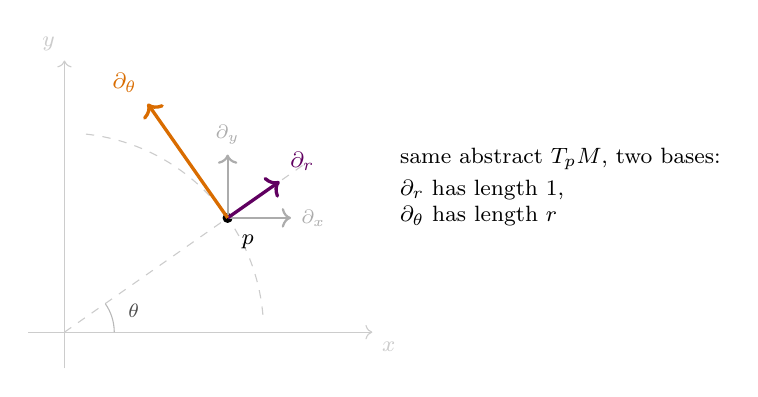
\begin{tikzpicture}[scale=1.15]
\draw[gray!40,->] (-0.4,0) -- (3.4,0) node[anchor=north west,font=\footnotesize]{$x$};
\draw[gray!40,->] (0,-0.4) -- (0,3.0) node[anchor=south east,font=\footnotesize]{$y$};
\draw[gray!40,dashed] (0,0) -- (35:3.3);
\draw[gray!40,dashed] (5:2.2) arc (5:85:2.2);
\draw[gray!55] (0.55,0) arc (0:35:0.55); \node[gray!60!black,font=\scriptsize] at (17:0.8) {$\theta$};
\fill (35:2.2) circle (1.6pt);
\node[font=\footnotesize,anchor=north west] at ($(35:2.2)+(0.05,-0.08)$) {$p$};
\draw[gray!65,->,thick] (35:2.2) -- ++(0.7,0) node[anchor=west,font=\scriptsize]{$\partial_x$};
\draw[gray!65,->,thick] (35:2.2) -- ++(0,0.7) node[anchor=south,font=\scriptsize]{$\partial_y$};
\draw[violet!75!black,->,very thick] (35:2.2) -- ++(35:0.7) node[anchor=south west,font=\footnotesize]{$\partial_r$};
\draw[orange!85!black,->,very thick] (35:2.2) -- ++(125:1.54) node[anchor=south east,font=\footnotesize]{$\partial_\theta$};
\node[font=\footnotesize,align=left,anchor=west] at (3.6,1.6) {same abstract $T_pM$, two bases:\\[2pt] $\partial_r$ has length $1$,\\ $\partial_\theta$ has length $r$};
\end{tikzpicture}
\end{center}

At a point $p$ at radius $r$, the four coordinate derivations --- elements of the abstract tangent space $T_pM$ --- drawn as the vectors of $T^{\geo}_pM = \mathbb{R}^2$ they correspond to under the identification $\partial_x \leftrightarrow e_1$, $\partial_y \leftrightarrow e_2$ of Proposition~\ref{prop:differential-agree} below (all at the common scale $0.7$). The polar ones are the radial and tangential directions, but $\partial_\theta$ is not a unit vector: it has length $r$, because it records the velocity of the curve $\theta \mapsto (r\cos\theta, r\sin\theta)$ along which the other coordinate is held fixed. A coordinate vector depends on the whole chart, not only on its own coordinate function --- the same abstract tangent space, and a different matrix for every map out of it.

\begin{propbox}[Agreement with the Vector-Space Differential]\thmlabel{prop:differential-agree}
Let $W \subseteq \mathbb{R}^m$ be open, $F : W \to \mathbb{R}^n$ smooth, and $a \in W$, and identify the abstract tangent spaces $T_aW \cong \mathbb{R}^m$ and $T_{F(a)}\mathbb{R}^n \cong \mathbb{R}^n$ by $\partial/\partial r^i \mapsto e_i$ --- that is, with the geometric tangent spaces $T^{\geo}_aW = \mathbb{R}^m$ and $T^{\geo}_{F(a)}\mathbb{R}^n = \mathbb{R}^n$. Then $F_{*a}$ corresponds to the Jacobian $F'(a)$, i.e.\ to the differential $dF_a$ of \S\ref{sub:vs-differential}. Under the same identification, $v = \sum_i v^i e_i$ corresponds to the derivation
\[
[g] \longmapsto \sum_i v^i\, \frac{\partial g}{\partial r^i}(a) = \frac{d}{dt}\Big|_{t=0} g(a + tv),
\]
the directional derivative $D_v$ of \S\ref{sub:derivations-motivation}.
\leeref{Proposition 3.13 and Corollary 3.3}
\end{propbox}

\begin{proof}
Apply Theorem~\ref{lem:differential-matrix} with the identity charts: then $\tilde F = F$, and the matrix of $F_{*a}$ is $F'(a)$. The second statement is the chain rule applied to $t \mapsto g(a + tv)$.
\end{proof}

\begin{corbox}[The Tangent Space to a Vector Space]\thmlabel{cor:tangent-vs}
Let $V$ be a finite-dimensional vector space with its standard smooth structure, and $a \in V$. The map
\[
V \to T_aV, \qquad v \mapsto D_v|_a, \qquad D_v|_a[f] = \frac{d}{dt}\Big|_{t=0} f(a + tv),
\]
is a linear isomorphism, defined without any choice of basis. For every linear map $L : V \to W$, $L_{*a}(D_v|_a) = D_{Lv}|_{La}$.
\leeref{Proposition 3.13}
\end{corbox}

\begin{proof}
For linear $L$, $L_{*a}(D_v|_a)[g] = D_v|_a[g \circ L] = \frac{d}{dt}\big|_0\, g(La + t\,Lv) = D_{Lv}|_{La}[g]$. Now take $L = L_0 : V \to \mathbb{R}^m$ a linear coordinate system. It is a chart, hence a diffeomorphism (Proposition~\ref{prop:chart-diffeo}), so $(L_0)_{*a}$ is an isomorphism, and it carries $D_v|_a$ to $D_{L_0 v}|_{L_0 a}$, which is $\sum_i (L_0 v)^i\,\partial/\partial r^i$ by Proposition~\ref{prop:differential-agree}. The composite $v \mapsto L_0 v \mapsto \sum_i (L_0v)^i\,\partial/\partial r^i$ is an isomorphism, hence so is $v \mapsto D_v|_a$. The defining formula mentions no basis.
\end{proof}

\begin{rembox}\label{rem:abstract-tangent-8}
This is what licenses the shared notation $dF_p$: on open subsets of Euclidean spaces the abstract differential \emph{is} the Jacobian, and between vector spaces it is the map of Theorem~\ref{thm:vs-differential-curves}. It also closes a loop opened in \S\ref{sub:derivations-motivation}, where a tangent vector $v$ was traded for the operator $D_v$; in $\mathbb{R}^n$ that trade is exactly the identification $e_i \leftrightarrow \partial/\partial r^i$.
\end{rembox}

\begin{defbox}[Rank and Regular Values of a Smooth Map]\deflabel{def:manifold-regular}
Let $F : M \to N$ be a smooth map. The \textbf{rank} of $F$ at $p$ is the rank of the linear map $F_{*p} : T_pM \to T_{F(p)}N$ of abstract tangent spaces; by Theorem~\ref{lem:differential-matrix} it is the rank of the Jacobian of any coordinate representation. A point $p$ is a \textbf{regular point} of $F$ if $F_{*p}$ is surjective, and $c \in N$ is a \textbf{regular value} if every $p \in F^{-1}(c)$ is a regular point.
\leeref{Ch.~4 and Ch.~5, p.~105}
\end{defbox}

\begin{rembox}[The Map Is Intrinsic --- the Matrix Is Not]\label{rem:map-intrinsic-matrix-not}
Uribe's closing point. The linear map $F_{*p}$ is defined with no choices, but its matrix depends on both charts: by Corollary~\ref{cor:change-coords}, changing them multiplies the matrix on each side by the Jacobian of a transition function. So only properties of $F_{*p}$ that survive such changes --- its rank, kernel and image, injectivity and surjectivity --- are properties of $F$, which is why the definition above is phrased through $F_{*p}$ rather than through a matrix. By Proposition~\ref{prop:differential-agree} it agrees with Definition~\ref{def:regular-value} in the Euclidean case. A regular point is exactly a point at which $F$ is a \emph{submersion}, in the sense of Definition~\ref{def:submersion}; maps with bijective, surjective and injective differentials are the subject of \ref{sec:special-maps}.
\end{rembox}

\begin{propbox}[Regular Values Inside One Chart]\thmlabel{prop:regular-one-chart}
Let $F : M \to N$ be a smooth map between smooth manifolds of dimensions $m$ and $n$, and $c \in N$. Suppose there are smooth charts $(U, \varphi)$ of $M$ and $(V, \psi)$ of $N$ with
\[
F^{-1}(c) \subseteq U, \qquad c \in V, \qquad F(U) \subseteq V .
\]
Let $\tilde F = \psi \circ F \circ \varphi^{-1} : \varphi(U) \to \mathbb{R}^n$ be the coordinate representation of $F$, a smooth map on the open set $\varphi(U) \subseteq \mathbb{R}^m$, and put $\tilde c = \psi(c) \in \mathbb{R}^n$. Then:
\begin{enumerate}
    \item $\varphi$ restricts to a homeomorphism from the level set $F^{-1}(c) \subseteq M$ onto the Euclidean level set $\tilde F^{-1}(\tilde c) \subseteq \varphi(U)$;
    \item $c$ is a regular value of $F$ in the sense of Definition~\ref{def:manifold-regular} if and only if $\tilde c$ is a regular value of $\tilde F$ in the sense of Definition~\ref{def:regular-value};
    \item in that case $F^{-1}(c)$ is a topological manifold of dimension $m - n$.
\end{enumerate}
\end{propbox}

\begin{proof}
(1) Let $x \in \varphi(U)$ and $q = \varphi^{-1}(x) \in U$. Since $F(U) \subseteq V$ and $\psi$ is injective on $V$,
\[
\tilde F(x) = \tilde c \iff \psi\big(F(q)\big) = \psi(c) \iff F(q) = c .
\]
So $\varphi\big(F^{-1}(c) \cap U\big) = \tilde F^{-1}(\tilde c)$, and $F^{-1}(c) \cap U = F^{-1}(c)$ by hypothesis. A homeomorphism restricts to a homeomorphism from any subset onto its image, both with the subspace topology.

(2) Let $p \in F^{-1}(c)$. By Theorem~\ref{lem:differential-matrix}, the matrix of $F_{*p}$ in the coordinate bases of the two charts is the Jacobian $\tilde F'(\varphi(p))$, and a linear map is surjective exactly when its matrix has rank equal to the dimension of the target (Proposition~\ref{fact:linalg}). So $p$ is a regular point of $F$ if and only if $\varphi(p)$ is a regular point of $\tilde F$. By (1), $p$ runs over $F^{-1}(c)$ exactly as $\varphi(p)$ runs over $\tilde F^{-1}(\tilde c)$.

(3) By (2) and Corollary~\ref{cor:rvt-open}, applied on the open set $\varphi(U) \subseteq \mathbb{R}^m$ with $k = n$, the Euclidean level set $\tilde F^{-1}(\tilde c)$ is a topological manifold of dimension $m - n$. By (1), $F^{-1}(c)$ is homeomorphic to it, and being a topological manifold is preserved by homeomorphisms.
\end{proof}

\begin{center}
\begin{tikzcd}[row sep=3em, column sep=4.4em]
F^{-1}(c) \subseteq U \arrow[r, "F"] \arrow[d, "\varphi"', "\cong"] & \{c\} \subseteq V \arrow[d, "\psi"] \\
\tilde F^{-1}(\tilde c) \subseteq \varphi(U) \arrow[r, "\tilde F"'] & \{\tilde c\} \subseteq \psi(V)
\end{tikzcd}
\end{center}

The proposition in one square. The level set upstairs is carried by the chart onto a level set downstairs, in Euclidean space, and the question ``is $c$ regular?'' is carried with it: surjectivity of $F_{*p}$ upstairs is the rank of $\tilde F'$ downstairs.

\begin{rembox}[The Strategy]\label{rem:strategy}
To show that $c$ is a regular value of a map between manifolds, and to see its level set:
\begin{enumerate}
    \item \emph{Locate the level set.} Show that $F^{-1}(c)$ lies inside a single chart domain $U$, and that $F(U)$ lies in a chart domain $V$ around $c$.
    \item \emph{Go downstairs.} Write the coordinate representation $\tilde F = \psi \circ F \circ \varphi^{-1}$, an ordinary map between open subsets of Euclidean spaces.
    \item \emph{Compute as in \ref{sec:rvt}.} Check that the Jacobian of $\tilde F$ has full rank $n$ at every point of the Euclidean level set $\tilde F^{-1}(\tilde c)$.
    \item \emph{Come back up.} By Proposition~\ref{prop:regular-one-chart}, $c$ is a regular value of $F$, and $F^{-1}(c)$ is homeomorphic, through the chart, to a Euclidean regular level set: a manifold of dimension $\dim M - \dim N$.
\end{enumerate}
Assignment~3, Problem~4 is exactly this. For the moment map $F : \mathbb{CP}^n \to \mathbb{R}^n$ and $c$ in the interior of the simplex, every point of $F^{-1}(c)$ has all homogeneous coordinates nonzero, so $F^{-1}(c) \subseteq U_0$ (step 1). The target chart is the identity of $\mathbb{R}^n$, and $\varphi_0(U_0) = \mathbb{C}^n \cong \mathbb{R}^{2n}$, so $\tilde F$ is an explicit rational map $\mathbb{R}^{2n} \to \mathbb{R}^n$ (step 2). Its Jacobian has rank $n$ on the level set (step 3). So the fibre is an $n$-dimensional manifold (step 4) --- in this case a regular level set of $\mathbb{R}^{2n}$ itself, exactly the situation of \ref{sec:rvt}. When a level set does not fit in one chart, the same argument applies around each of its points separately, as the next corollary shows.
\end{rembox}

Complex projective space through the course: the open quotient $S^{2n+1}/S^1$, Hausdorff, second countable and compact, in Section~\ref{sec:ex-cpn}; the circle group $\Ugp(1)$ acting there in Example~\ref{ex:1-circle}; an orbit space in Example~\ref{ex:cpn-orbit}; a smooth and complex manifold through its standard atlas in Section~\ref{sec:projective-smooth}; a homogeneous space of $\Ugp(n+1)$ in Remark~\ref{rem:dimension-checks-through-homogeneous-spaces}; the domain of the moment map in Remark~\ref{rem:strategy}; and the base of the Hopf fibration in Section~\ref{sec:ex-hopf}.


\begin{corbox}[Regular Level Sets Are Topological Manifolds]\thmlabel{cor:manifold-level-sets}
Let $F : M \to N$ be a smooth map between smooth manifolds of dimensions $m$ and $n$, and $c \in N$ a regular value of $F$. Then $F^{-1}(c)$, with the subspace topology, is a topological manifold of dimension $m - n$ (or empty).
\end{corbox}

\begin{proof}
Hausdorffness and second countability are inherited from $M$ (Theorem~\ref{thm:subspace-inherit}). For local Euclideanness, let $p \in F^{-1}(c)$. Choose smooth charts $(V, \psi)$ around $c$ and $(U_0, \varphi_0)$ around $p$, and put $U = U_0 \cap F^{-1}(V)$, an open neighbourhood of $p$ because $F$ is continuous; restricting $\varphi_0$ gives a smooth chart $(U, \varphi)$ (Lemma~\ref{lem:chart-modify}). Apply Proposition~\ref{prop:regular-one-chart} to the restriction $F|_U : U \to N$, a smooth map on the open submanifold $U$: its level set $F^{-1}(c) \cap U$ lies in $U$, it maps $U$ into $V$, and $c$ is still a regular value, since $T_qU = T_qM$ and $(F|_U)_{*q} = F_{*q}$ for $q \in U$ (Lemma~\ref{lem:germs-local}). So $F^{-1}(c) \cap U$, an open neighbourhood of $p$ in $F^{-1}(c)$, is a topological manifold of dimension $m - n$; in particular $p$ has a neighbourhood in $F^{-1}(c)$ homeomorphic to an open subset of $\mathbb{R}^{m-n}$.
\end{proof}

This is the topological half of the regular value theorem for manifolds, and it is \ref{sec:rvt} applied chart by chart. The smooth half --- that $F^{-1}(c)$ is a smooth \emph{submanifold} of $M$, with tangent space $\ker F_{*p}$ --- came in Lecture~12, as Theorem~\ref{thm:rvt-manifolds}, proved with the local normal form for submersions (Theorem~\ref{thm:submersion-normal-form}): near each point of the level set, $F$ is a projection, so the level set is a coordinate slice. It is Lee's Corollary~5.14 and Proposition~5.38. The corollary above is now a consequence of it, a submanifold being in particular a topological manifold, but its proof --- \ref{sec:rvt} applied chart by chart --- is more elementary.

\begin{propbox}[Maps with Zero Differential Are Constant]\thmlabel{prop:zero-differential}
Let $F : M \to N$ be smooth, with $M$ connected. If $F_{*p} = 0$ for every $p \in M$, then $F$ is constant.
\end{propbox}

\begin{proof}
\textit{(Assignment~4, Problem~1: the submitted solution, condensed.)} \emph{$F$ is locally constant.} Fix $p_0 \in M$. Take a chart $(V, \psi)$ at $F(p_0)$ and a chart at $p_0$ whose domain $U_0$ satisfies $F(U_0) \subseteq V$ and whose image is an open ball $B$ --- shrink by continuity of $F$, then to a ball. The coordinate representation $\tilde F = \psi \circ F \circ \varphi^{-1} : B \to \mathbb{R}^n$ has Jacobian $\tilde F'(\varphi(p))$, the matrix of $F_{*p}$ (Theorem~\ref{lem:differential-matrix}), so $\tilde F' \equiv 0$ on $B$. For $p \in U_0$, the segment from $\varphi(p_0)$ to $\varphi(p)$ stays in the convex $B$, and the mean value theorem applied to each component of $\tilde F$ along it gives $\tilde F(\varphi(p)) = \tilde F(\varphi(p_0))$; since $\psi$ is injective, $F(p) = F(p_0)$.

\emph{$F$ is constant.} Let $c = F(p_0)$. The set $F^{-1}(c)$ is closed, since $F$ is continuous, and open, since $F$ is locally constant; it is nonempty. As $M$ is connected, $F^{-1}(c) = M$.
\end{proof}

The hypothesis that $M$ is connected cannot be dropped: on a disconnected $M$, a map that takes different constant values on different components has zero differential everywhere. Locally, the proposition is the familiar fact from calculus that a function with zero derivative on an interval is constant.

% ============================================================================
% SECTION: TANGENT VECTORS AS VELOCITIES OF CURVES
% ============================================================================

\section{Tangent Vectors as Velocities of Curves}\label{sec:velocities}\label{sub:velocities}

\roadmark{Stage: abstract}{The other face of a tangent vector: every derivation is the velocity of a curve, on every manifold. Tangent spaces of products split.}

\textit{Assignment 3, Problem 2.} Tangent vectors were introduced with two faces: velocities of curves, and derivations (the remark at the start of \S\ref{sub:derivations}). For regular level sets the two were identified by Theorem~\ref{thm:ambient-abstract}, through the ambient space. This section identifies them on \emph{every} smooth manifold, with no ambient space at all.

\begin{defbox}[Smooth Curve and Its Velocity]\deflabel{def:velocity}
Let $J \subseteq \mathbb{R}$ be an open interval containing $0$, with its standard smooth structure and coordinate $t$. A \textbf{smooth curve} in $M$ is a smooth map $\gamma : J \to M$. If $\gamma(0) = p$, the \textbf{velocity} of $\gamma$ at $0$ is the abstract tangent vector
\[
D_\gamma = \gamma_{*0}\Big(\frac{d}{dt}\Big|_0\Big) \in T_pM, \qquad\text{explicitly}\qquad D_\gamma[f] = \frac{d}{dt}\Big|_{t=0} f\big(\gamma(t)\big).
\]
\leeref{Ch.~3, \emph{Velocity Vectors of Curves}}
\end{defbox}

The explicit formula is the definition of the pushforward: $\gamma_{*0}(d/dt|_0)[f] = d/dt|_0\,[f \circ \gamma]$, the ordinary derivative at $0$ of the function $f \circ \gamma$, which is defined near $0$. Lee writes $\gamma'(0)$ for $D_\gamma$. These notes keep $\gamma'(0)$ for the ordinary derivative of a curve in $\mathbb{R}^N$, which is a \emph{geometric} tangent vector, and write $D_\gamma$ for the abstract one, as Assignment~3 does.

\begin{propbox}[Velocity in Coordinates]\thmlabel{prop:velocity-coords}
$D_\gamma$ is a derivation at $p$. In a chart $(U, \varphi)$ at $p$ with coordinate functions $x^1, \ldots, x^n$,
\[
D_\gamma = \sum_{j=1}^n \big(x^j \circ \gamma\big)'(0)\, \frac{\partial}{\partial x^j}\Big|_p .
\]
In particular $D_\gamma$ depends only on the velocity $(\varphi \circ \gamma)'(0) \in \mathbb{R}^n$ of the coordinate curve $\varphi \circ \gamma$.
\leeref{Ch.~3, \emph{Velocity Vectors of Curves}}
\end{propbox}

\begin{proof}
$D_\gamma$ is a pushforward of a derivation, hence a derivation (Proposition~\ref{prop:pushforward-derivation}) --- which is why Assignment~3 could waive the check. By the universal formula (Theorem~\ref{thm:tangent-basis}), the $j$-th coefficient of $D_\gamma$ is $D_\gamma[x^j] = (x^j \circ \gamma)'(0)$.
\end{proof}

The same formula comes out of the chain rule directly, as in the assignment's solution. With $c = \varphi \circ \gamma$ and $c^j = r^j \circ c = x^j \circ \gamma$, near $0$ one has $f \circ \gamma = f_\varphi \circ c$, so
\[
D_\gamma[f] = \frac{d}{dt}\Big|_0 f_\varphi\big(c(t)\big) = \sum_{j} \frac{\partial f_\varphi}{\partial r^j}\big(\varphi(p)\big)\,(c^j)'(0) = \sum_j (c^j)'(0)\,\frac{\partial}{\partial x^j}\Big|_p[f].
\]
Each input $r^j$ of $f_\varphi$ moves at speed $(c^j)'(0)$ along the curve, and contributes $\partial f_\varphi/\partial r^j \cdot (c^j)'(0)$ to the rate of change.

\begin{thmbox}[Every Tangent Vector Is a Velocity]\thmlabel{thm:every-vector-velocity}
For every $D \in T_pM$ there is a smooth curve $\gamma : (-\varepsilon, \varepsilon) \to M$ with $\gamma(0) = p$ and $D_\gamma = D$.
\leeref{Proposition 3.23}
\end{thmbox}

\begin{proof}
\textit{(Assignment 3, Problem 2.)} Fix a chart $(U, \varphi)$ at $p$ with coordinate functions $x^i$, and put $a^i = D[x^i]$ and $a = (a^1, \ldots, a^n) \in \mathbb{R}^n$. These are the coefficients of $D$ in the universal formula; the freedom lies in the curve.

\emph{The curve downstairs.} Let $c(t) = \varphi(p) + t\,a$. Since $\varphi(U)$ is open, some ball $B(\varphi(p), r)$ lies in it. If $a \ne 0$ take $\varepsilon = r/|a|$, so that $|c(t) - \varphi(p)| = |t|\,|a| < r$ for $|t| < \varepsilon$. If $a = 0$, which happens exactly when $D = 0$, take $\varepsilon = 1$. In either case $c : (-\varepsilon, \varepsilon) \to \varphi(U)$ is smooth, being affine, with $c(0) = \varphi(p)$ and $c'(0) = a$.

\emph{The curve upstairs.} Let $\gamma = \varphi^{-1} \circ c$. It is smooth, since its coordinate representation in the chart $(U,\varphi)$ is $\varphi \circ \gamma = c$, and $\gamma(0) = p$. Its coordinate curve is $\varphi \circ \gamma = c$, so $(x^j \circ \gamma)'(0) = (c^j)'(0) = a^j$.

\emph{Conclusion.} By Proposition~\ref{prop:velocity-coords} and the universal formula,
\[
D_\gamma = \sum_j a^j\, \frac{\partial}{\partial x^j}\Big|_p = \sum_j D[x^j]\, \frac{\partial}{\partial x^j}\Big|_p = D. \qedhere
\]
\end{proof}

Assignment~3's solution first treats the basis vectors $\partial/\partial x^i|_p$, using curves with $c'(0) = e_i$, and then the general case. The general argument contains the basis case, with $a = e_i$ and $c(t) = \varphi(p) + t\,e_i$, so it is presented here alone.

\begin{corbox}[Velocity of a Composite --- Computing Differentials by Curves]\thmlabel{cor:velocity-composite}
Let $F : M \to N$ be smooth and $\gamma$ a smooth curve in $M$ with $\gamma(0) = p$. Then $D_{F \circ \gamma} = F_{*p}(D_\gamma)$. Consequently, for every $D \in T_pM$,
\[
F_{*p}(D) = D_{F \circ \gamma} \qquad \text{for any smooth curve } \gamma \text{ with } \gamma(0) = p \text{ and } D_\gamma = D,
\]
and such a curve exists by Theorem~\ref{thm:every-vector-velocity}.
\leeref{Proposition 3.24 and Corollary 3.25}
\end{corbox}

\begin{proof}
By the Chain Rule (Theorem~\ref{prop:pushforward-functorial}), $D_{F \circ \gamma} = (F \circ \gamma)_{*0}(d/dt|_0) = F_{*p}\big(\gamma_{*0}(d/dt|_0)\big) = F_{*p}(D_\gamma)$.
\end{proof}

This is Lee's main computational tool: to find $F_{*p}(D)$, choose any curve with velocity $D$ and differentiate $F$ along it. It is the manifold version of Theorem~\ref{thm:vs-differential-curves}, and it is how Lee computes the differential of the determinant (Problem~7-4).

\begin{center}
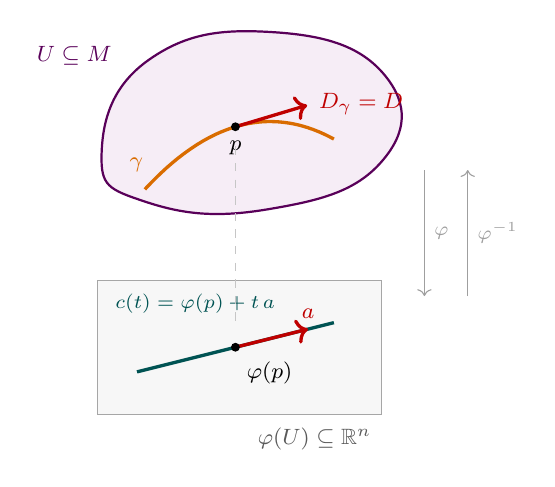
\begin{tikzpicture}
\draw[violet!70!black,fill=violet!7,thick] plot[smooth cycle,tension=0.8] coordinates {(0.9,3.05) (1.5,4.25) (3.1,4.6) (4.5,4.05) (4.45,2.95) (3.0,2.35) (1.45,2.45)};
\draw[orange!85!black,very thick] (1.450,2.605) -- (1.480,2.638) -- (1.511,2.670) -- (1.541,2.701) -- (1.572,2.732) -- (1.602,2.762) -- (1.632,2.791) -- (1.663,2.820) -- (1.693,2.848) -- (1.723,2.876) -- (1.754,2.903) -- (1.784,2.929) -- (1.815,2.955) -- (1.845,2.980) -- (1.875,3.004) -- (1.906,3.028) -- (1.936,3.051) -- (1.966,3.073) -- (1.997,3.095) -- (2.027,3.117) -- (2.058,3.137) -- (2.088,3.157) -- (2.118,3.177) -- (2.149,3.195) -- (2.179,3.214) -- (2.209,3.231) -- (2.240,3.248) -- (2.270,3.264) -- (2.301,3.280) -- (2.331,3.295) -- (2.361,3.309) -- (2.392,3.323) -- (2.422,3.336) -- (2.453,3.348) -- (2.483,3.360) -- (2.513,3.371) -- (2.544,3.382) -- (2.574,3.392) -- (2.604,3.401) -- (2.635,3.410) -- (2.665,3.418) -- (2.696,3.426) -- (2.726,3.432) -- (2.756,3.439) -- (2.787,3.444) -- (2.817,3.449) -- (2.847,3.453) -- (2.878,3.457) -- (2.908,3.460) -- (2.939,3.463) -- (2.969,3.464) -- (2.999,3.466) -- (3.030,3.466) -- (3.060,3.466) -- (3.091,3.465) -- (3.121,3.464) -- (3.151,3.462) -- (3.182,3.459) -- (3.212,3.456) -- (3.242,3.452) -- (3.273,3.448) -- (3.303,3.443) -- (3.334,3.437) -- (3.364,3.431) -- (3.394,3.424) -- (3.425,3.416) -- (3.455,3.408) -- (3.485,3.399) -- (3.516,3.390) -- (3.546,3.379) -- (3.577,3.369) -- (3.607,3.357) -- (3.637,3.345) -- (3.668,3.333) -- (3.698,3.319) -- (3.728,3.306) -- (3.759,3.291) -- (3.789,3.276) -- (3.820,3.260) -- (3.850,3.244);
\draw[red!75!black,->,very thick] (2.600,3.400) -- (3.510,3.673);
\node[red!75!black,font=\footnotesize,anchor=west] at (3.540,3.693) {$D_\gamma = D$};
\fill (2.600,3.400) circle (1.6pt); \node[font=\footnotesize,anchor=north] at (2.600,3.340) {$p$};
\node[orange!85!black,font=\footnotesize,anchor=south east] at (1.550,2.710) {$\gamma$};
\node[violet!70!black,font=\footnotesize,anchor=east] at (1.15,4.3) {$U \subseteq M$};
\draw[gray!70,fill=gray!6] (0.85,-0.25) rectangle (4.45,1.45);
\draw[teal!65!black,very thick] (1.350,0.287) -- (3.850,0.912);
\draw[red!75!black,->,very thick] (2.600,0.600) -- (3.522,0.830) node[anchor=south,font=\footnotesize]{$a$};
\fill (2.600,0.600) circle (1.6pt); \node[font=\footnotesize,anchor=north west] at (2.620,0.540) {$\varphi(p)$};
\node[teal!65!black,font=\scriptsize,anchor=north west] at (0.95,1.4) {$c(t) = \varphi(p) + t\,a$};
\node[gray!70!black,font=\footnotesize,anchor=north east] at (4.45,-0.3) {$\varphi(U) \subseteq \mathbb{R}^n$};
\draw[->,gray!75] (5.0,2.85) -- node[right,font=\scriptsize]{$\varphi$} (5.0,1.25);
\draw[->,gray!75] (5.55,1.25) -- node[right,font=\scriptsize]{$\varphi^{-1}$} (5.55,2.85);
\draw[gray!45,dashed] (2.600,3.150) -- (2.600,0.850);
\end{tikzpicture}
\end{center}

The proof in one picture. Downstairs, in the chart, the curve is the straight line through $\varphi(p)$ in the direction of the coefficient vector $a = (D[x^1], \ldots, D[x^n])$. The chart carries it upstairs to a curve $\gamma$ in $M$, bent by whatever distortion $\varphi^{-1}$ introduces. The bending is invisible to the velocity, which depends only on $(\varphi \circ \gamma)'(0) = a$ --- so the velocity is $D$.

\begin{center}
\begin{tikzcd}[row sep=3em, column sep=3.6em]
& U \subseteq M \arrow[d, "\varphi"] \\
(-\varepsilon, \varepsilon) \arrow[ur, "\gamma = \varphi^{-1} \circ c"] \arrow[r, "c"'] & \varphi(U) \subseteq \mathbb{R}^n
\end{tikzcd}
\end{center}

The same construction as a diagram: the curve is built downstairs as $c$ and lifted by $\varphi^{-1}$, and the triangle commutes, $\varphi \circ \gamma = c$.

\begin{rembox}[The Two Faces Reconciled]\label{rem:two-faces-reconciled}
Theorem~\ref{thm:every-vector-velocity} says the map $\gamma \mapsto D_\gamma$, from smooth curves through $p$ to $T_pM$, is onto. By Proposition~\ref{prop:velocity-coords}, two curves have the same velocity exactly when their coordinate curves have the same velocity in one chart, and then in every chart. So $T_pM$ may equally be described as \emph{curves through $p$, modulo having the same velocity in coordinates} --- the intrinsic ``velocities of curves'' definition of the tangent space, now a theorem, on every manifold, with no ambient space. For a regular level set, the abstract velocity $D_\gamma$ is the derivation $D_{\gamma'(0)}$ attached to the geometric velocity $\gamma'(0) \in T^{\geo}_pM$ (Proposition~\ref{prop:Dv-properties}(2)). So the identification of Theorem~\ref{thm:ambient-abstract} is the statement that the two notions of velocity agree.
\end{rembox}

\subsection{Tangent Spaces of Products}\label{sub:tangent-products}

\textit{Lecture 11. ``There is a natural isomorphism'' between the tangent space of a product and the direct sum of the tangent spaces of the factors --- ``natural meaning coordinate-free.'' Uribe gave three ways to see it: by the inclusions of the factors, by curves, and in coordinates. He added that this part of the course is, in his experience, ``the most abstract, somehow the hardest part'', and that while physicists tend to favour coordinates and pure mathematicians abstract settings, ``you need both.''}

Throughout, $p = (p_1, p_2) \in M_1 \times M_2$, and $\iota_1 = \iota^{p_2} : M_1 \to M_1 \times M_2$, $\iota_2 = \iota^{p_1} : M_2 \to M_1 \times M_2$ are the slice inclusions through $p$ (Definition~\ref{def:product-manifold}).

\begin{thmbox}[The Tangent Space of a Product]\thmlabel{thm:tangent-product}
The linear map
\[
\Theta : T_{p_1}M_1 \oplus T_{p_2}M_2 \longrightarrow T_p(M_1 \times M_2), \qquad \Theta(v, w) = \iota_{1*}v + \iota_{2*}w,
\]
is an isomorphism, defined without charts, with inverse $\Psi(D) = (\pi_{1*}D, \pi_{2*}D)$. In particular $\iota_{1*}$ and $\iota_{2*}$ are injective, and $T_p(M_1 \times M_2)$ is the internal direct sum of their images, $\Theta\big(T_{p_1}M_1 \oplus \{0\}\big)$ and $\Theta\big(\{0\} \oplus T_{p_2}M_2\big)$.
\leeref{Proposition 3.14}
\end{thmbox}

\begin{proof}
\textit{(Stated in lecture; Uribe left the injectivity as ``check''.)} First, the pushforward along a constant map is zero: if $\kappa$ is constant with value $q_0$ and $[g]$ is a germ at $q_0$, then $g \circ \kappa$ is constant, so $(\kappa_* D)[g] = D[g \circ \kappa] = 0$ because derivations kill constants (Lemma~\ref{lem:derivation-properties}). Now $\pi_1 \circ \iota_1 = \mathrm{id}_{M_1}$ and $\pi_2 \circ \iota_2 = \mathrm{id}_{M_2}$, while $\pi_2 \circ \iota_1$ and $\pi_1 \circ \iota_2$ are constant. By the Chain Rule (Theorem~\ref{prop:pushforward-functorial}),
\[
\pi_{1*}\iota_{1*} = \mathrm{id}, \qquad \pi_{2*}\iota_{2*} = \mathrm{id}, \qquad \pi_{2*}\iota_{1*} = 0, \qquad \pi_{1*}\iota_{2*} = 0,
\]
so $\Psi(\Theta(v, w)) = (v, w)$, and $\Theta$ is injective. Both spaces have dimension $m_1 + m_2$ (Theorem~\ref{thm:tangent-basis} and Propositions~\ref{prop:product-manifold}, \ref{prop:direct-sum}), so $\Theta$ is an isomorphism (Proposition~\ref{fact:linalg}(1)) with inverse $\Psi$. The last sentence is Proposition~\ref{prop:direct-sum}(1), carried across $\Theta$.
\end{proof}

\begin{center}
\begin{tikzcd}[column sep=4.6em, row sep=2.4em]
M_1 \arrow[r, shift left=0.8ex, "\iota_1"] & M_1 \times M_2 \arrow[l, shift left=0.8ex, "\pi_1"] \arrow[r, shift right=0.8ex, "\pi_2"'] & M_2 \arrow[l, shift right=0.8ex, "\iota_2"']
\end{tikzcd}
\qquad\qquad
\begin{tikzcd}[column sep=4.6em]
T_{p_1}M_1 \oplus T_{p_2}M_2 \arrow[r, shift left=0.8ex, "\Theta"] & T_p(M_1 \times M_2) \arrow[l, shift left=0.8ex, "\Psi"]
\end{tikzcd}
\end{center}

The slice inclusions and the projections through $p$. The four identities $\pi_1 \iota_1 = \mathrm{id}$, $\pi_2 \iota_2 = \mathrm{id}$, and $\pi_2 \iota_1$, $\pi_1 \iota_2$ constant, pushed forward to tangent spaces, are the whole proof that $\Psi \circ \Theta = \mathrm{id}$.

\textbf{Partial derivatives in the $M_1$ variables.} For $v \in T_{p_1}M_1$ and a germ $[f]$ at $p$,
\[
(\iota_{1*}v)[f] = v\big[f \circ \iota_1\big], \qquad (f \circ \iota_1)(q) = f(q, p_2) :
\]
to push $v$ forward, restrict $f$ to the slice $M_1 \times \{p_2\}$ and differentiate there. So the first summand consists of derivations ``only with respect to the $M_1$ variables'', with $p_2$ held fixed --- partial derivatives in the direction of $M_1$ --- and the second of partial derivatives in the direction of $M_2$.

\begin{center}
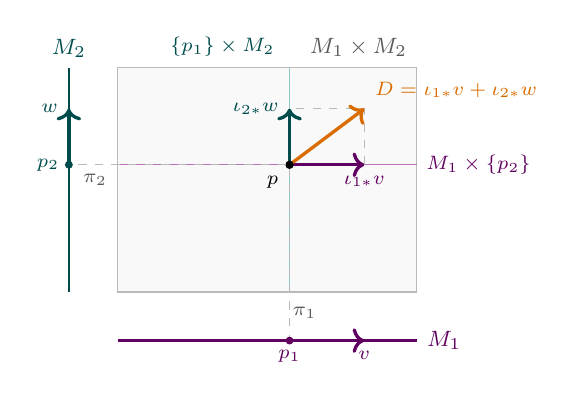
\begin{tikzpicture}[scale=0.95]
\fill[gray!5] (0,0) rectangle (4,3); \draw[gray!55] (0,0) rectangle (4,3); \node[font=\footnotesize, gray!70!black, anchor=south east] at (4,3.02) {$M_1 \times M_2$};
\draw[violet!75!black, thick] (0,-0.65) -- (4,-0.65) node[right, font=\footnotesize] {$M_1$};
\draw[teal!60!black, thick] (-0.65,0) -- (-0.65,3) node[above, font=\footnotesize] {$M_2$};
\draw[violet!55] (0,1.70) -- (4,1.70) node[right, font=\scriptsize, text=violet!75!black] {$M_1 \times \{p_2\}$};
\draw[teal!45] (2.30,0) -- (2.30,3);  \node[font=\scriptsize, text=teal!60!black, anchor=south] at (1.40,3.02) {$\{p_1\} \times M_2$};
\draw[gray!55, dashed] (3.30,1.70) -- (3.30,2.45) -- (2.30,2.45);
\draw[->, very thick, violet!75!black] (2.30,1.70) -- (3.30,1.70) node[below, font=\scriptsize] {$\iota_{1*}v$};
\draw[->, very thick, teal!60!black] (2.30,1.70) -- (2.30,2.45) node[left, font=\scriptsize] {$\iota_{2*}w$};
\draw[->, very thick, orange!85!black] (2.30,1.70) -- (3.30,2.45) node[above right, font=\scriptsize] {$D = \iota_{1*}v + \iota_{2*}w$};
\fill (2.30,1.70) circle (1.6pt); \node[font=\scriptsize, anchor=north east] at (2.28,1.68) {$p$};
\draw[gray!55, dashed] (2.30,1.65) -- (2.30,-0.65); \draw[gray!55, dashed] (2.25,1.70) -- (-0.65,1.70);
\fill[violet!75!black] (2.30,-0.65) circle (1.5pt) node[below, font=\scriptsize] {$p_1$}; \draw[->, very thick, violet!75!black] (2.30,-0.65) -- (3.30,-0.65) node[below, font=\scriptsize] {$v$};
\fill[teal!60!black] (-0.65,1.70) circle (1.5pt) node[left, font=\scriptsize] {$p_2$}; \draw[->, very thick, teal!60!black] (-0.65,1.70) -- (-0.65,2.45) node[left, font=\scriptsize] {$w$};
\node[font=\scriptsize, gray!70!black] at (2.50,-0.28) {$\pi_1$}; \node[font=\scriptsize, gray!70!black] at (-0.3,1.50) {$\pi_2$};
\end{tikzpicture}
\end{center}

The isomorphism in one picture. Through $p$ run the two slices, $M_1 \times \{p_2\}$ and $\{p_1\} \times M_2$. Pushing $v$ and $w$ forward along the slice inclusions gives tangent vectors along the slices, and every $D \in T_p(M_1 \times M_2)$ is uniquely their sum. The projections take $D$ back to $v$ and $w$: $\Psi(D) = (\pi_{1*}D, \pi_{2*}D) = (v, w)$.

\begin{corbox}[Product Coordinates]\thmlabel{cor:tangent-product-coords}
In product coordinates $(x^1, \ldots, x^{m_1}, y^1, \ldots, y^{m_2})$ at $p$,
\[
\iota_{1*}\Big(\frac{\partial}{\partial x^i}\Big|_{p_1}\Big) = \frac{\partial}{\partial x^i}\Big|_p, \qquad \iota_{2*}\Big(\frac{\partial}{\partial y^j}\Big|_{p_2}\Big) = \frac{\partial}{\partial y^j}\Big|_p .
\]
So the $\partial/\partial x^i|_p$ form a basis of the first summand and the $\partial/\partial y^j|_p$ a basis of the second.
\leeref{Proposition 3.14}
\end{corbox}

\begin{proof}
By Proposition~\ref{prop:product-maps} the coordinate representation of $\iota_1$ is $r \mapsto (r, \varphi_2(p_2))$, with Jacobian $\binom{I_{m_1}}{0}$. By Theorem~\ref{lem:differential-matrix} its $i$-th column says $\iota_{1*}(\partial/\partial x^i|_{p_1}) = \partial/\partial x^i|_p$. The same for $\iota_2$.
\end{proof}

\begin{corbox}[Velocities of Curves in a Product]\thmlabel{cor:tangent-product-curves}
Let $\gamma = (\gamma_1, \gamma_2)$ be a smooth curve in $M_1 \times M_2$ with $\gamma(0) = p$. Then $\Psi(D_\gamma) = (D_{\gamma_1}, D_{\gamma_2})$, that is, $D_\gamma = \iota_{1*}D_{\gamma_1} + \iota_{2*}D_{\gamma_2}$. In particular, if $\gamma_2$ is constant --- a ``horizontal'' curve $\gamma(t) = (\gamma_1(t), p_2)$ --- then $D_\gamma = \iota_{1*}D_{\gamma_1}$ lies in the first summand.
\end{corbox}

\begin{proof}
$\gamma_i = \pi_i \circ \gamma$, so $\pi_{i*}D_\gamma = D_{\pi_i \circ \gamma} = D_{\gamma_i}$ by Corollary~\ref{cor:velocity-composite}. If $\gamma_2$ is constant, $D_{\gamma_2} = 0$.
\end{proof}

This is the second of Uribe's three views, and it uses the velocities of Assignment~3, Problem~2 (\ref{sub:velocities}).

\section{The Cotangent Space}\label{sec:cotangent}

\roadmark{Stage: abstract, dual}{Differentials of functions and the cotangent space: defined as a dual, then recovered from germs alone.}

% ============================================================================
% Lecture 10 (Wed Sep 23, 2026)
% ============================================================================
\subsection{Differentials of Functions and the Cotangent Space}\label{sub:cotangent}

\textit{Lecture 10: ``a very special case --- a very important case.'' The target is $N = \mathbb{R}$, and the differential of a scalar function becomes a covector.}

On $\mathbb{R}$ we always use the standard coordinate $r$. For every $c \in \mathbb{R}$ the abstract tangent space $T_c\mathbb{R}$ has the basis $\{\partial/\partial r|_c\}$ (Theorem~\ref{thm:tangent-basis}), and we identify $T_c\mathbb{R} \cong \mathbb{R}$ once and for all by $\partial/\partial r|_c \mapsto 1$ --- ``we identify this with $\mathbb{R}$ forever.''

\begin{defbox}[Cotangent Space]\deflabel{def:cotangent}
Let $M$ be a smooth manifold and $p \in M$. The \textbf{cotangent space} of $M$ at $p$ is the dual of the abstract tangent space,
\[
T_p^*M = (T_pM)^* .
\]
\leeref{Ch.~11, \emph{Covectors}}
\end{defbox}

\begin{defbox}[The Differential of a Function]\deflabel{def:differential-function}
Let $M$ be a smooth manifold and $p \in M$. For a smooth $f : M \to \mathbb{R}$ (or one defined only near $p$), the \textbf{differential} of $f$ at $p$ is $df_p = f_{*p} : T_pM \to T_{f(p)}\mathbb{R} \cong \mathbb{R}$. Here $T_{f(p)}\mathbb{R}$ is identified with $\mathbb{R}$ by $c\,\partial/\partial r|_{f(p)} \mapsto c$, the derivation $\partial/\partial r|_{f(p)}$ being a basis (Theorem~\ref{thm:tangent-basis}). So $df_p$ takes a tangent vector $D \in T_pM$ and returns a number, $df_p(D) = D[f]$ (Proposition~\ref{prop:df-derivation}); it is linear, so $df_p \in T_p^*M$, the cotangent space of Definition~\ref{def:cotangent}.
\leeref{Ch.~11, \emph{Covectors}}
\end{defbox}

\begin{center}
\begin{tikzcd}[column sep=4.4em, row sep=2.6em]
T_pM \arrow[r, "f_{*p}"] \arrow[rr, bend right=22, "df_p"'] & T_{f(p)}\mathbb{R} \arrow[r, "\partial_r \,\mapsto\, 1", "\cong"'] & \mathbb{R}
\end{tikzcd}
\end{center}

The differential of a function is its pushforward followed by the permanent identification of every tangent space of $\mathbb{R}$ with $\mathbb{R}$; so $df_p$ is the pushforward $f_{*p}$ under another name. The notation $T_p^*M$ puts the star on the $T$ ``to save some ink.''

\begin{propbox}[The Differential Evaluates Derivations]\thmlabel{prop:df-derivation}
For every $D \in T_pM$, $\ df_p(D) = D[f]$. In particular $df_p\big(\partial/\partial x^j|_p\big) = \partial f/\partial x^j(p)$ in any chart.
\leeref{Ch.~11, \emph{Covectors}}
\end{propbox}

\begin{proof}
By the universal formula at $f(p)$ with the coordinate $r$, $f_{*p}D = (f_{*p}D)[r]\,\partial/\partial r|_{f(p)}$, and $(f_{*p}D)[r] = D[r \circ f] = D[f]$. Under the identification, $\partial/\partial r|_{f(p)} \mapsto 1$.
\end{proof}

\begin{lembox}[The Differential in Coordinates]\thmlabel{lem:df-coords}
Let $(x^1, \ldots, x^m)$ be coordinates near $p$, and write $dx^i|_p$ for the differential at $p$ of the coordinate function $x^i$. Then $\{dx^1|_p, \ldots, dx^m|_p\}$ is the dual basis of $\{\partial/\partial x^1|_p, \ldots, \partial/\partial x^m|_p\}$, so $\dim T_p^*M = m$ (Proposition~\ref{prop:dual-basis}), and for every smooth $f$ defined near $p$,
\[
df_p = \sum_{i=1}^m \frac{\partial f}{\partial x^i}(p)\, dx^i\big|_p .
\]
\leeref{Ch.~11, \emph{Covectors}}
\end{lembox}

\begin{proof}
\textit{(Lecture~10: ``it suffices to check the identity on basis vectors.'' In lecture the left side came from the matrix of $f_{*p}$ (Theorem~\ref{lem:differential-matrix}), a $1 \times m$ row --- ``remember, gradients are across'', after a student first proposed $m \times 1$ --- whose $j$-th entry is $\partial f/\partial x^j(p)$. Proposition~\ref{prop:df-derivation} gives the same value directly.)} By Proposition~\ref{prop:df-derivation}, $dx^i|_p(\partial/\partial x^j|_p) = \partial x^i/\partial x^j(p) = \partial r^i/\partial r^j = \delta^i_j$, which is the defining property of the dual basis (Definition~\ref{def:dual}). Two linear functionals agree if they agree on a basis (Proposition~\ref{fact:linalg}(2)), so it suffices to evaluate both sides of the formula on $\partial/\partial x^j|_p$. The left side gives $\partial f/\partial x^j(p)$, again by Proposition~\ref{prop:df-derivation}; the right side gives $\sum_i \partial f/\partial x^i(p)\,\delta^i_j = \partial f/\partial x^j(p)$.
\end{proof}

\begin{corbox}[Components of a Covector]\thmlabel{cor:covector-components}
In a chart $(x^1, \ldots, x^m)$ near $p$, every covector $\alpha \in T_p^*M$ is
\[
\alpha = \sum_{j=1}^m a_j\, dx^j\big|_p, \qquad a_j = \alpha\Big(\frac{\partial}{\partial x^j}\Big|_p\Big) .
\]
The numbers $a_1, \ldots, a_m$ are the \textbf{components} of $\alpha$ in the chart.
\leeref{Ch.~11, \emph{Covectors}}
\end{corbox}

\begin{proof}
\textit{(Lecture~15 recalled the basis $dx^j|_p$ --- ``a fact that I forgot to mention to remind you'' --- and read off the components by evaluation.)} By Lemma~\ref{lem:df-coords} the $dx^j|_p$ form the basis of $T_p^*M$ dual to the $\partial/\partial x^j|_p$, and Proposition~\ref{prop:dual-basis} expands every element of a dual space in the dual basis with the coefficients $\alpha(\partial/\partial x^j|_p)$.
\end{proof}

\begin{corbox}[Properties of the Differential of a Function]\thmlabel{cor:df-properties}
Let $f, g$ be smooth near $p$ and $a, b \in \mathbb{R}$. Then
\[
d(af + bg)_p = a\,df_p + b\,dg_p, \qquad d(fg)_p = f(p)\,dg_p + g(p)\,df_p,
\]
and if $h$ is smooth on an open interval containing the values of $f$ near $p$, then $d(h \circ f)_p = h'(f(p))\,df_p$.
\leeref{Proposition 11.20}
\end{corbox}

\begin{proof}
Evaluate at $D \in T_pM$ using Proposition~\ref{prop:df-derivation}. The first two identities are the linearity and the Leibniz rule of $D$. For the third, $D[h \circ f] = (f_{*p}D)[h]$, and under the identification of Definition~\ref{def:cotangent}, $f_{*p}D = df_p(D)\,\partial/\partial r|_{f(p)}$; applying this to $h$ gives $df_p(D)\,h'(f(p))$.
\end{proof}

\begin{rembox}\label{rem:cotangent}
Equivalently, by Theorem~\ref{lem:differential-matrix} with the coordinate $r$ on the target, the matrix of $f_{*p}$ is the $1 \times m$ row
\[
\Big( \frac{\partial f}{\partial x^1}(p) \ \ \cdots \ \ \frac{\partial f}{\partial x^m}(p) \Big).
\]
A student proposed $m \times 1$; it is $1 \times m$ --- ``gradients go across'' --- since the target is one-dimensional. The lecture's proof took this route and paused over the shape of the matrix; the version above goes through Proposition~\ref{prop:df-derivation} instead, which avoids the question.
\end{rembox}

\begin{center}
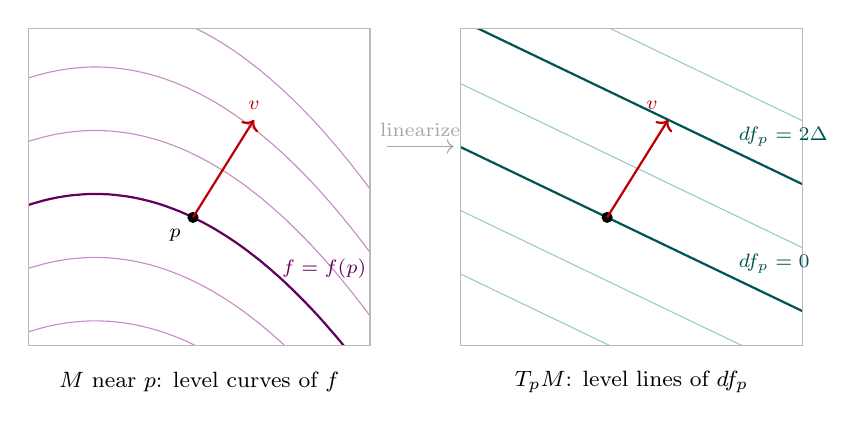
\begin{tikzpicture}
\begin{scope}[scale=1.55]
\begin{scope}\clip (-0.55,-1.05) rectangle (2.25,1.55);
\draw[violet!45] (-0.600,-0.956) -- (-0.576,-0.947) -- (-0.551,-0.939) -- (-0.527,-0.931) -- (-0.503,-0.924) -- (-0.478,-0.917) -- (-0.454,-0.910) -- (-0.429,-0.903) -- (-0.405,-0.897) -- (-0.381,-0.891) -- (-0.356,-0.886) -- (-0.332,-0.881) -- (-0.308,-0.876) -- (-0.283,-0.872) -- (-0.259,-0.868) -- (-0.234,-0.864) -- (-0.210,-0.861) -- (-0.186,-0.858) -- (-0.161,-0.856) -- (-0.137,-0.854) -- (-0.113,-0.852) -- (-0.088,-0.850) -- (-0.064,-0.849) -- (-0.039,-0.848) -- (-0.015,-0.848) -- (0.009,-0.848) -- (0.034,-0.848) -- (0.058,-0.849) -- (0.082,-0.850) -- (0.107,-0.851) -- (0.131,-0.853) -- (0.155,-0.855) -- (0.180,-0.858) -- (0.204,-0.861) -- (0.229,-0.864) -- (0.253,-0.867) -- (0.277,-0.871) -- (0.302,-0.875) -- (0.326,-0.880) -- (0.350,-0.885) -- (0.375,-0.890) -- (0.399,-0.896) -- (0.424,-0.902) -- (0.448,-0.908) -- (0.472,-0.915) -- (0.497,-0.922) -- (0.521,-0.929) -- (0.545,-0.937) -- (0.570,-0.945) -- (0.594,-0.954) -- (0.618,-0.963) -- (0.643,-0.972) -- (0.667,-0.982) -- (0.692,-0.991) -- (0.716,-1.002) -- (0.740,-1.012) -- (0.765,-1.023) -- (0.789,-1.035) -- (0.813,-1.047) -- (0.838,-1.059) -- (0.862,-1.071) -- (0.887,-1.084) -- (0.911,-1.097) -- (0.935,-1.110) -- (0.960,-1.124) -- (0.984,-1.138) -- (1.008,-1.153) -- (1.033,-1.168) -- (1.057,-1.183) -- (1.082,-1.199) -- (1.106,-1.215) -- (1.130,-1.231) -- (1.155,-1.248) -- (1.179,-1.265) -- (1.203,-1.282) -- (1.228,-1.300) -- (1.252,-1.318) -- (1.276,-1.337) -- (1.301,-1.356) -- (1.325,-1.375) -- (1.350,-1.394) -- (1.374,-1.414) -- (1.398,-1.435) -- (1.423,-1.455) -- (1.447,-1.476) -- (1.471,-1.498) -- (1.496,-1.519) -- (1.520,-1.541) -- (1.545,-1.564) -- (1.569,-1.586) -- (1.593,-1.610) -- (1.618,-1.633) -- (1.642,-1.657) -- (1.666,-1.681) -- (1.691,-1.706) -- (1.715,-1.730) -- (1.739,-1.756) -- (1.764,-1.781) -- (1.788,-1.807) -- (1.813,-1.834) -- (1.837,-1.860) -- (1.861,-1.887) -- (1.886,-1.915) -- (1.910,-1.943) -- (1.934,-1.971) -- (1.959,-1.999) -- (1.983,-2.028) -- (2.008,-2.057) -- (2.032,-2.087) -- (2.056,-2.117) -- (2.081,-2.147) -- (2.105,-2.177) -- (2.129,-2.208) -- (2.154,-2.240) -- (2.178,-2.271) -- (2.203,-2.303) -- (2.227,-2.336) -- (2.251,-2.368) -- (2.276,-2.402) -- (2.300,-2.435);
\draw[violet!45] (-0.600,-0.436) -- (-0.576,-0.427) -- (-0.551,-0.419) -- (-0.527,-0.411) -- (-0.503,-0.404) -- (-0.478,-0.397) -- (-0.454,-0.390) -- (-0.429,-0.383) -- (-0.405,-0.377) -- (-0.381,-0.371) -- (-0.356,-0.366) -- (-0.332,-0.361) -- (-0.308,-0.356) -- (-0.283,-0.352) -- (-0.259,-0.348) -- (-0.234,-0.344) -- (-0.210,-0.341) -- (-0.186,-0.338) -- (-0.161,-0.336) -- (-0.137,-0.334) -- (-0.113,-0.332) -- (-0.088,-0.330) -- (-0.064,-0.329) -- (-0.039,-0.328) -- (-0.015,-0.328) -- (0.009,-0.328) -- (0.034,-0.328) -- (0.058,-0.329) -- (0.082,-0.330) -- (0.107,-0.331) -- (0.131,-0.333) -- (0.155,-0.335) -- (0.180,-0.338) -- (0.204,-0.341) -- (0.229,-0.344) -- (0.253,-0.347) -- (0.277,-0.351) -- (0.302,-0.355) -- (0.326,-0.360) -- (0.350,-0.365) -- (0.375,-0.370) -- (0.399,-0.376) -- (0.424,-0.382) -- (0.448,-0.388) -- (0.472,-0.395) -- (0.497,-0.402) -- (0.521,-0.409) -- (0.545,-0.417) -- (0.570,-0.425) -- (0.594,-0.434) -- (0.618,-0.443) -- (0.643,-0.452) -- (0.667,-0.462) -- (0.692,-0.471) -- (0.716,-0.482) -- (0.740,-0.492) -- (0.765,-0.503) -- (0.789,-0.515) -- (0.813,-0.527) -- (0.838,-0.539) -- (0.862,-0.551) -- (0.887,-0.564) -- (0.911,-0.577) -- (0.935,-0.590) -- (0.960,-0.604) -- (0.984,-0.618) -- (1.008,-0.633) -- (1.033,-0.648) -- (1.057,-0.663) -- (1.082,-0.679) -- (1.106,-0.695) -- (1.130,-0.711) -- (1.155,-0.728) -- (1.179,-0.745) -- (1.203,-0.762) -- (1.228,-0.780) -- (1.252,-0.798) -- (1.276,-0.817) -- (1.301,-0.836) -- (1.325,-0.855) -- (1.350,-0.874) -- (1.374,-0.894) -- (1.398,-0.915) -- (1.423,-0.935) -- (1.447,-0.956) -- (1.471,-0.978) -- (1.496,-0.999) -- (1.520,-1.021) -- (1.545,-1.044) -- (1.569,-1.066) -- (1.593,-1.090) -- (1.618,-1.113) -- (1.642,-1.137) -- (1.666,-1.161) -- (1.691,-1.186) -- (1.715,-1.210) -- (1.739,-1.236) -- (1.764,-1.261) -- (1.788,-1.287) -- (1.813,-1.314) -- (1.837,-1.340) -- (1.861,-1.367) -- (1.886,-1.395) -- (1.910,-1.423) -- (1.934,-1.451) -- (1.959,-1.479) -- (1.983,-1.508) -- (2.008,-1.537) -- (2.032,-1.567) -- (2.056,-1.597) -- (2.081,-1.627) -- (2.105,-1.657) -- (2.129,-1.688) -- (2.154,-1.720) -- (2.178,-1.751) -- (2.203,-1.783) -- (2.227,-1.816) -- (2.251,-1.848) -- (2.276,-1.882) -- (2.300,-1.915);
\draw[violet!75!black,thick] (-0.600,0.084) -- (-0.576,0.093) -- (-0.551,0.101) -- (-0.527,0.109) -- (-0.503,0.116) -- (-0.478,0.123) -- (-0.454,0.130) -- (-0.429,0.137) -- (-0.405,0.143) -- (-0.381,0.149) -- (-0.356,0.154) -- (-0.332,0.159) -- (-0.308,0.164) -- (-0.283,0.168) -- (-0.259,0.172) -- (-0.234,0.176) -- (-0.210,0.179) -- (-0.186,0.182) -- (-0.161,0.184) -- (-0.137,0.186) -- (-0.113,0.188) -- (-0.088,0.190) -- (-0.064,0.191) -- (-0.039,0.192) -- (-0.015,0.192) -- (0.009,0.192) -- (0.034,0.192) -- (0.058,0.191) -- (0.082,0.190) -- (0.107,0.189) -- (0.131,0.187) -- (0.155,0.185) -- (0.180,0.182) -- (0.204,0.179) -- (0.229,0.176) -- (0.253,0.173) -- (0.277,0.169) -- (0.302,0.165) -- (0.326,0.160) -- (0.350,0.155) -- (0.375,0.150) -- (0.399,0.144) -- (0.424,0.138) -- (0.448,0.132) -- (0.472,0.125) -- (0.497,0.118) -- (0.521,0.111) -- (0.545,0.103) -- (0.570,0.095) -- (0.594,0.086) -- (0.618,0.077) -- (0.643,0.068) -- (0.667,0.058) -- (0.692,0.049) -- (0.716,0.038) -- (0.740,0.028) -- (0.765,0.017) -- (0.789,0.005) -- (0.813,-0.007) -- (0.838,-0.019) -- (0.862,-0.031) -- (0.887,-0.044) -- (0.911,-0.057) -- (0.935,-0.070) -- (0.960,-0.084) -- (0.984,-0.098) -- (1.008,-0.113) -- (1.033,-0.128) -- (1.057,-0.143) -- (1.082,-0.159) -- (1.106,-0.175) -- (1.130,-0.191) -- (1.155,-0.208) -- (1.179,-0.225) -- (1.203,-0.242) -- (1.228,-0.260) -- (1.252,-0.278) -- (1.276,-0.297) -- (1.301,-0.316) -- (1.325,-0.335) -- (1.350,-0.354) -- (1.374,-0.374) -- (1.398,-0.395) -- (1.423,-0.415) -- (1.447,-0.436) -- (1.471,-0.458) -- (1.496,-0.479) -- (1.520,-0.501) -- (1.545,-0.524) -- (1.569,-0.546) -- (1.593,-0.570) -- (1.618,-0.593) -- (1.642,-0.617) -- (1.666,-0.641) -- (1.691,-0.666) -- (1.715,-0.690) -- (1.739,-0.716) -- (1.764,-0.741) -- (1.788,-0.767) -- (1.813,-0.794) -- (1.837,-0.820) -- (1.861,-0.847) -- (1.886,-0.875) -- (1.910,-0.903) -- (1.934,-0.931) -- (1.959,-0.959) -- (1.983,-0.988) -- (2.008,-1.017) -- (2.032,-1.047) -- (2.056,-1.077) -- (2.081,-1.107) -- (2.105,-1.137) -- (2.129,-1.168) -- (2.154,-1.200) -- (2.178,-1.231) -- (2.203,-1.263) -- (2.227,-1.296) -- (2.251,-1.328) -- (2.276,-1.362) -- (2.300,-1.395);
\draw[violet!45] (-0.600,0.604) -- (-0.576,0.613) -- (-0.551,0.621) -- (-0.527,0.629) -- (-0.503,0.636) -- (-0.478,0.643) -- (-0.454,0.650) -- (-0.429,0.657) -- (-0.405,0.663) -- (-0.381,0.669) -- (-0.356,0.674) -- (-0.332,0.679) -- (-0.308,0.684) -- (-0.283,0.688) -- (-0.259,0.692) -- (-0.234,0.696) -- (-0.210,0.699) -- (-0.186,0.702) -- (-0.161,0.704) -- (-0.137,0.706) -- (-0.113,0.708) -- (-0.088,0.710) -- (-0.064,0.711) -- (-0.039,0.712) -- (-0.015,0.712) -- (0.009,0.712) -- (0.034,0.712) -- (0.058,0.711) -- (0.082,0.710) -- (0.107,0.709) -- (0.131,0.707) -- (0.155,0.705) -- (0.180,0.702) -- (0.204,0.699) -- (0.229,0.696) -- (0.253,0.693) -- (0.277,0.689) -- (0.302,0.685) -- (0.326,0.680) -- (0.350,0.675) -- (0.375,0.670) -- (0.399,0.664) -- (0.424,0.658) -- (0.448,0.652) -- (0.472,0.645) -- (0.497,0.638) -- (0.521,0.631) -- (0.545,0.623) -- (0.570,0.615) -- (0.594,0.606) -- (0.618,0.597) -- (0.643,0.588) -- (0.667,0.578) -- (0.692,0.569) -- (0.716,0.558) -- (0.740,0.548) -- (0.765,0.537) -- (0.789,0.525) -- (0.813,0.513) -- (0.838,0.501) -- (0.862,0.489) -- (0.887,0.476) -- (0.911,0.463) -- (0.935,0.450) -- (0.960,0.436) -- (0.984,0.422) -- (1.008,0.407) -- (1.033,0.392) -- (1.057,0.377) -- (1.082,0.361) -- (1.106,0.345) -- (1.130,0.329) -- (1.155,0.312) -- (1.179,0.295) -- (1.203,0.278) -- (1.228,0.260) -- (1.252,0.242) -- (1.276,0.223) -- (1.301,0.204) -- (1.325,0.185) -- (1.350,0.166) -- (1.374,0.146) -- (1.398,0.125) -- (1.423,0.105) -- (1.447,0.084) -- (1.471,0.062) -- (1.496,0.041) -- (1.520,0.019) -- (1.545,-0.004) -- (1.569,-0.026) -- (1.593,-0.050) -- (1.618,-0.073) -- (1.642,-0.097) -- (1.666,-0.121) -- (1.691,-0.146) -- (1.715,-0.170) -- (1.739,-0.196) -- (1.764,-0.221) -- (1.788,-0.247) -- (1.813,-0.274) -- (1.837,-0.300) -- (1.861,-0.327) -- (1.886,-0.355) -- (1.910,-0.383) -- (1.934,-0.411) -- (1.959,-0.439) -- (1.983,-0.468) -- (2.008,-0.497) -- (2.032,-0.527) -- (2.056,-0.557) -- (2.081,-0.587) -- (2.105,-0.617) -- (2.129,-0.648) -- (2.154,-0.680) -- (2.178,-0.711) -- (2.203,-0.743) -- (2.227,-0.776) -- (2.251,-0.808) -- (2.276,-0.842) -- (2.300,-0.875);
\draw[violet!45] (-0.600,1.124) -- (-0.576,1.133) -- (-0.551,1.141) -- (-0.527,1.149) -- (-0.503,1.156) -- (-0.478,1.163) -- (-0.454,1.170) -- (-0.429,1.177) -- (-0.405,1.183) -- (-0.381,1.189) -- (-0.356,1.194) -- (-0.332,1.199) -- (-0.308,1.204) -- (-0.283,1.208) -- (-0.259,1.212) -- (-0.234,1.216) -- (-0.210,1.219) -- (-0.186,1.222) -- (-0.161,1.224) -- (-0.137,1.226) -- (-0.113,1.228) -- (-0.088,1.230) -- (-0.064,1.231) -- (-0.039,1.232) -- (-0.015,1.232) -- (0.009,1.232) -- (0.034,1.232) -- (0.058,1.231) -- (0.082,1.230) -- (0.107,1.229) -- (0.131,1.227) -- (0.155,1.225) -- (0.180,1.222) -- (0.204,1.219) -- (0.229,1.216) -- (0.253,1.213) -- (0.277,1.209) -- (0.302,1.205) -- (0.326,1.200) -- (0.350,1.195) -- (0.375,1.190) -- (0.399,1.184) -- (0.424,1.178) -- (0.448,1.172) -- (0.472,1.165) -- (0.497,1.158) -- (0.521,1.151) -- (0.545,1.143) -- (0.570,1.135) -- (0.594,1.126) -- (0.618,1.117) -- (0.643,1.108) -- (0.667,1.098) -- (0.692,1.089) -- (0.716,1.078) -- (0.740,1.068) -- (0.765,1.057) -- (0.789,1.045) -- (0.813,1.033) -- (0.838,1.021) -- (0.862,1.009) -- (0.887,0.996) -- (0.911,0.983) -- (0.935,0.970) -- (0.960,0.956) -- (0.984,0.942) -- (1.008,0.927) -- (1.033,0.912) -- (1.057,0.897) -- (1.082,0.881) -- (1.106,0.865) -- (1.130,0.849) -- (1.155,0.832) -- (1.179,0.815) -- (1.203,0.798) -- (1.228,0.780) -- (1.252,0.762) -- (1.276,0.743) -- (1.301,0.724) -- (1.325,0.705) -- (1.350,0.686) -- (1.374,0.666) -- (1.398,0.645) -- (1.423,0.625) -- (1.447,0.604) -- (1.471,0.582) -- (1.496,0.561) -- (1.520,0.539) -- (1.545,0.516) -- (1.569,0.494) -- (1.593,0.470) -- (1.618,0.447) -- (1.642,0.423) -- (1.666,0.399) -- (1.691,0.374) -- (1.715,0.350) -- (1.739,0.324) -- (1.764,0.299) -- (1.788,0.273) -- (1.813,0.246) -- (1.837,0.220) -- (1.861,0.193) -- (1.886,0.165) -- (1.910,0.137) -- (1.934,0.109) -- (1.959,0.081) -- (1.983,0.052) -- (2.008,0.023) -- (2.032,-0.007) -- (2.056,-0.037) -- (2.081,-0.067) -- (2.105,-0.097) -- (2.129,-0.128) -- (2.154,-0.160) -- (2.178,-0.191) -- (2.203,-0.223) -- (2.227,-0.256) -- (2.251,-0.288) -- (2.276,-0.322) -- (2.300,-0.355);
\draw[violet!45] (-0.600,1.644) -- (-0.576,1.653) -- (-0.551,1.661) -- (-0.527,1.669) -- (-0.503,1.676) -- (-0.478,1.683) -- (-0.454,1.690) -- (-0.429,1.697) -- (-0.405,1.703) -- (-0.381,1.709) -- (-0.356,1.714) -- (-0.332,1.719) -- (-0.308,1.724) -- (-0.283,1.728) -- (-0.259,1.732) -- (-0.234,1.736) -- (-0.210,1.739) -- (-0.186,1.742) -- (-0.161,1.744) -- (-0.137,1.746) -- (-0.113,1.748) -- (-0.088,1.750) -- (-0.064,1.751) -- (-0.039,1.752) -- (-0.015,1.752) -- (0.009,1.752) -- (0.034,1.752) -- (0.058,1.751) -- (0.082,1.750) -- (0.107,1.749) -- (0.131,1.747) -- (0.155,1.745) -- (0.180,1.742) -- (0.204,1.739) -- (0.229,1.736) -- (0.253,1.733) -- (0.277,1.729) -- (0.302,1.725) -- (0.326,1.720) -- (0.350,1.715) -- (0.375,1.710) -- (0.399,1.704) -- (0.424,1.698) -- (0.448,1.692) -- (0.472,1.685) -- (0.497,1.678) -- (0.521,1.671) -- (0.545,1.663) -- (0.570,1.655) -- (0.594,1.646) -- (0.618,1.637) -- (0.643,1.628) -- (0.667,1.618) -- (0.692,1.609) -- (0.716,1.598) -- (0.740,1.588) -- (0.765,1.577) -- (0.789,1.565) -- (0.813,1.553) -- (0.838,1.541) -- (0.862,1.529) -- (0.887,1.516) -- (0.911,1.503) -- (0.935,1.490) -- (0.960,1.476) -- (0.984,1.462) -- (1.008,1.447) -- (1.033,1.432) -- (1.057,1.417) -- (1.082,1.401) -- (1.106,1.385) -- (1.130,1.369) -- (1.155,1.352) -- (1.179,1.335) -- (1.203,1.318) -- (1.228,1.300) -- (1.252,1.282) -- (1.276,1.263) -- (1.301,1.244) -- (1.325,1.225) -- (1.350,1.206) -- (1.374,1.186) -- (1.398,1.165) -- (1.423,1.145) -- (1.447,1.124) -- (1.471,1.102) -- (1.496,1.081) -- (1.520,1.059) -- (1.545,1.036) -- (1.569,1.014) -- (1.593,0.990) -- (1.618,0.967) -- (1.642,0.943) -- (1.666,0.919) -- (1.691,0.894) -- (1.715,0.870) -- (1.739,0.844) -- (1.764,0.819) -- (1.788,0.793) -- (1.813,0.766) -- (1.837,0.740) -- (1.861,0.713) -- (1.886,0.685) -- (1.910,0.657) -- (1.934,0.629) -- (1.959,0.601) -- (1.983,0.572) -- (2.008,0.543) -- (2.032,0.513) -- (2.056,0.483) -- (2.081,0.453) -- (2.105,0.423) -- (2.129,0.392) -- (2.154,0.360) -- (2.178,0.329) -- (2.203,0.297) -- (2.227,0.264) -- (2.251,0.232) -- (2.276,0.198) -- (2.300,0.165);
\end{scope}
\draw[gray!55] (-0.55,-1.05) rectangle (2.25,1.55);
\fill (0.800,0.000) circle (1.3pt);
\node[font=\scriptsize,anchor=north east] at (0.780,-0.020) {$p$};
\draw[red!75!black,->,thick] (0.800,0.000) -- (1.300,0.800) node[anchor=south,font=\scriptsize]{$v$};
\node[violet!75!black,font=\scriptsize,anchor=west] at (1.45,-0.419) {$f = f(p)$};
\node[font=\footnotesize] at (0.85,-1.35) {$M$ near $p$: level curves of $f$};
\end{scope}
\begin{scope}[xshift=6.5cm,scale=1.55]
\begin{scope}\clip (-1.2,-1.05) rectangle (1.6,1.55);
\draw[teal!40] (-1.300,-0.416) -- (1.700,-1.856);
\draw[teal!40] (-1.300,0.104) -- (1.700,-1.336);
\draw[teal!65!black,thick] (-1.300,0.624) -- (1.700,-0.816);
\draw[teal!40] (-1.300,1.144) -- (1.700,-0.296);
\draw[teal!65!black,thick] (-1.300,1.664) -- (1.700,0.224);
\draw[teal!40] (-1.300,2.184) -- (1.700,0.744);
\end{scope}
\draw[gray!55] (-1.2,-1.05) rectangle (1.6,1.55);
\fill (0,0) circle (1.3pt);
\draw[red!75!black,->,thick] (0,0) -- (0.500,0.800) node[anchor=south east,font=\scriptsize]{$v$};
\node[teal!65!black,font=\scriptsize,anchor=south west,inner sep=1pt] at (1.050,-0.484) {$df_p = 0$};
\node[teal!65!black,font=\scriptsize,anchor=south west,inner sep=1pt] at (1.050,0.556) {$df_p = 2\Delta$};
\node[font=\footnotesize] at (0.2,-1.35) {$T_pM$: level lines of $df_p$};
\end{scope}
\draw[->,gray!70] (3.7,0.9) -- node[above,font=\scriptsize]{linearize} (4.55,0.9);
\end{tikzpicture}
\end{center}

The differential as a covector, for $f(x,y) = y + 0.3x^2$ near $p = (0.8, 0)$. Left: level curves of $f$ at equal spacing $\Delta$, and a tangent vector $v$ at $p$. Right: in $T_pM$, the level lines of the linear functional $df_p$ at the same spacing --- the linearization of the curves on the left, straight and parallel. The value $df_p(v)$ counts, in units of $\Delta$, how many lines $v$ crosses: here exactly $2\Delta$, since $v$ ends on the line $df_p = 2\Delta$. On the left, $v$ crosses \emph{approximately} two level curves; the curvature is what the linearization discards.

\begin{rembox}[Differential --- Not Gradient]\label{rem:differential-not-gradient}
``The standard formula from Calc 3 now has this manifold general interpretation.'' The formula $df = \sum \partial f/\partial x^i\,dx^i$ of multivariable calculus is now a statement about covectors: the $dx^i|_p$ are not infinitesimals but the dual basis of the coordinate derivations, the coefficients are numbers, and the dual basis ``extracts the components of a vector in the original basis.'' What does \emph{not} survive on a manifold is the gradient. A function on $M$ has no gradient \emph{vector} --- converting $df_p$ into a vector requires an inner product on $T_pM$, i.e.\ a Riemannian metric --- but it always has its differential $df_p \in T_p^*M$, and that is where differentials of scalar functions live. Differential forms, later in the term, will be built from covectors, and will pull back as naturally as germs do. Uribe also announced that tangent vectors, written $D$ while thought of as derivations, will soon be written $v$.
\end{rembox}

\subsection{The Cotangent Space from Germs}\label{sub:cotangent-germs}

\textit{Assignment 3, Problem 3. The cotangent space was defined in Lecture 10 as the dual $(T_pM)^*$. This subsection shows that it also has a description with no dualizing at all, in terms of germs alone --- ``as you can see, it has the natural definition $I_p/I_p^2$.'' The proof splits into four results: a characterization of $I_p^2$, a basis of the quotient, a non-degenerate pairing, and the isomorphism, which then comes from the Linear Algebra Toolkit for free.}

\begin{defbox}[The Space $I_p/I_p^2$]\deflabel{def:Ip-quotient}
$I_p/I_p^2$ is the quotient vector space (Definition~\ref{def:quotient-vs}) of $I_p$ by its subspace $I_p^2$ (Lemma~\ref{lem:Ip-subspaces}). The class of $[f] \in I_p$ is written $[[f]] = [f] + I_p^2$, and $[[f]] = [[f']]$ iff $[f'] - [f] \in I_p^2$.
\end{defbox}

\begin{propbox}[Germs Vanishing to Second Order]\thmlabel{prop:second-order}
For $[f] \in C_p^\infty(M)$ the following are equivalent:
\begin{enumerate}
    \item $[f] \in I_p^2$;
    \item $f(p) = 0$ and $df_p = 0$;
    \item $f(p) = 0$ and $\partial f/\partial x^i(p) = 0$ for all $i$, in one --- hence every --- chart at $p$.
\end{enumerate}
\leeref{Problem 11-4(a)}
\end{propbox}

\begin{proof}
(2)$\iff$(3): by Lemma~\ref{lem:df-coords}, $df_p = \sum_i \partial f/\partial x^i(p)\,dx^i|_p$, and the $dx^i|_p$ form a basis. Condition (2) mentions no chart, which is why ``one'' chart implies ``every''.

(1)$\Rightarrow$(2): every element of $I_p^2$ lies in $I_p$, so it vanishes at $p$. And for $[u], [w] \in I_p$ and any $D \in T_pM$, Proposition~\ref{prop:df-derivation} and Lemma~\ref{lem:derivation-properties}(2) give $d(uw)_p(D) = D([u][w]) = 0$. So $d(uw)_p = 0$, and by linearity $df_p = 0$ for every $[f] \in I_p^2$.

(3)$\Rightarrow$(1): \textit{(Assignment 3, Problem 3.)} Fix a chart $(U,\varphi)$ at $p$, a representative $f : V \to \mathbb{R}$, and put $a = \varphi(p)$ and $f_\varphi = f \circ \varphi^{-1}$. The hypotheses say $f_\varphi(a) = 0$ and $\partial f_\varphi/\partial r^i(a) = 0$. On an open ball $B \subseteq \varphi(U \cap V)$ centred at $a$, Hadamard's lemma (Lemma~\ref{lem:hadamard}) gives smooth $f_i$ with
\[
f_\varphi(r) = \sum_{i=1}^n (r^i - a^i)\, f_i(r) \quad (r \in B), \qquad f_i(a) = \frac{\partial f_\varphi}{\partial r^i}(a) = 0 .
\]
On the open neighbourhood $W = \varphi^{-1}(B)$ of $p$, with $r = \varphi(q)$ and $r^i = x^i(q)$, this reads
\[
f(q) = \sum_{i=1}^n \big(x^i(q) - x^i(p)\big)\,(f_i \circ \varphi)(q) \qquad (q \in W),
\]
an identity of germs: $[f] = \sum_i [x^i - x^i(p)]\,[f_i \circ \varphi]$. Both factors of each term vanish at $p$ --- the second because $f_i(a) = 0$ --- so each term is a product of two elements of $I_p$, and $[f] \in I_p^2$.
\end{proof}

\begin{rembox}\label{rem:cotangent-2}
The proposition is the conceptual centre of Problem~3. $I_p$ consists of the germs vanishing to \emph{first} order at $p$, and $I_p^2$ of those vanishing to \emph{second} order --- value and first derivatives zero. So the quotient $I_p/I_p^2$ remembers exactly the first derivatives of a germ that vanishes at $p$, and nothing else. It only needs first-order Hadamard: the vanishing of $f_i(a)$ is what puts the second factor in $I_p$.
\end{rembox}

\begin{propbox}[A Basis of $I_p/I_p^2$]\thmlabel{prop:ideal-basis}
Let $(U, \varphi)$ be a chart at $p$ with coordinate functions $x^1, \ldots, x^n$. For every $[f] \in I_p$,
\[
[[f]] = \sum_{i=1}^n \frac{\partial f}{\partial x^i}(p)\, [[x^i - x^i(p)]],
\]
and the classes $[[x^1 - x^1(p)]], \ldots, [[x^n - x^n(p)]]$ form a basis of $I_p/I_p^2$. In particular $\dim I_p/I_p^2 = n$.
\leeref{cf.\ Problem 11-4(a)}
\end{propbox}

\begin{proof}
Each $x^i - x^i(p)$ is smooth on $U$ and vanishes at $p$, so its germ lies in $I_p$. Put $g = f - \sum_i \partial f/\partial x^i(p)\,(x^i - x^i(p))$ near $p$. Then $g(p) = 0$ and, using $\partial x^i/\partial x^j = \delta^i_j$,
\[
\frac{\partial g}{\partial x^j}(p) = \frac{\partial f}{\partial x^j}(p) - \sum_i \frac{\partial f}{\partial x^i}(p)\,\delta^i_j = 0,
\]
so $[g] \in I_p^2$ by Proposition~\ref{prop:second-order}. This is the displayed expansion, which shows that the classes span. For independence, suppose $\sum_i c_i\,[[x^i - x^i(p)]] = 0$, i.e.\ $\sum_i c_i\,[x^i - x^i(p)] \in I_p^2$. By Proposition~\ref{prop:second-order} its $j$-th partial at $p$ vanishes, and that partial is $c_j$.
\end{proof}

This is the cotangent counterpart of the basis theorem for $T_pM$ (Theorem~\ref{thm:tangent-basis}): the coefficients of $[[f]]$ are the first partials of $f$, just as the coefficients of a derivation $D$ were its values $D[x^i]$.

\begin{defbox}[The Pairing Between Tangent Vectors and $I_p/I_p^2$]\deflabel{def:cotangent-pairing}
The \textbf{pairing} of $T_pM$ with $I_p/I_p^2$ is
\[
\langle\ ,\ \rangle : T_pM \times I_p/I_p^2 \to \mathbb{R}, \qquad \langle D, [[f]] \rangle = D[f] .
\]
\end{defbox}

\begin{propbox}[The Pairing Is Well Defined and Non-Degenerate]\thmlabel{prop:cotangent-pairing}
The pairing of Definition~\ref{def:cotangent-pairing} is well defined, bilinear, and non-degenerate in the sense of Definition~\ref{def:pairing}.
\leeref{no counterpart; Lee proves Problem 11-4(b) without a pairing}
\end{propbox}

\begin{proof}
\emph{Well defined} \textit{(Problem~3(a))}. Each $D$ is a linear functional on $I_p$ that vanishes on $I_p^2$ (Lemma~\ref{lem:derivation-properties}(2)), so it descends to $I_p/I_p^2$ by the universal property of quotient spaces (Proposition~\ref{prop:quotient-vs}(2)). \emph{Bilinear:} derivations are linear, and they are added and scaled pointwise.

\emph{Left non-degenerate.} If $D[f] = 0$ for every $[f] \in I_p$, then $D = 0$, because a derivation is determined by its values on $I_p$ (Lemma~\ref{lem:derivation-properties}(1)).

\emph{Right non-degenerate.} If $[f] \in I_p$ and $D[f] = 0$ for every $D \in T_pM$, then $df_p = 0$ by Proposition~\ref{prop:df-derivation}; with $f(p) = 0$, Proposition~\ref{prop:second-order} gives $[f] \in I_p^2$, i.e.\ $[[f]] = 0$.
\end{proof}

\begin{thmbox}[The Cotangent Space from Germs]\thmlabel{thm:cotangent-ideal}
\begin{enumerate}
    \item The pairing induces isomorphisms
    \[
    T_pM \xrightarrow{\ \cong\ } \big(I_p/I_p^2\big)^*, \qquad\qquad \Phi : I_p/I_p^2 \xrightarrow{\ \cong\ } (T_pM)^* = T_p^*M .
    \]
    \item $\Phi([[f]]) = df_p$: the isomorphism sends the class of a germ to its differential.
    \item In any chart, $\Phi$ carries the basis $[[x^i - x^i(p)]]$ of $I_p/I_p^2$ to the basis $dx^i|_p$ of $T_p^*M$, which is dual to the basis $\partial/\partial x^i|_p$ of $T_pM$.
\end{enumerate}
The isomorphisms are defined without any chart.
\leeref{Problem 11-4(b), with global functions in place of germs (see the comparison below)}
\end{thmbox}

\begin{proof}
(1) $T_pM$ is finite-dimensional (Theorem~\ref{thm:tangent-basis}) and the pairing is non-degenerate (Proposition~\ref{prop:cotangent-pairing}), so Theorem~\ref{thm:pairing} applies. (2) $\Phi([[f]])(D) = \langle D, [[f]] \rangle = D[f] = df_p(D)$ by Proposition~\ref{prop:df-derivation}. (3) By (2), $\Phi([[x^i - x^i(p)]]) = d(x^i - x^i(p))_p = dx^i|_p$, since a constant has zero differential (Lemma~\ref{lem:derivation-properties}(1)); and the $dx^i|_p$ are dual to the $\partial/\partial x^i|_p$ by Lemma~\ref{lem:df-coords}. Every map in (1) is defined by $\langle D, [[f]] \rangle = D[f]$, which mentions no chart.
\end{proof}

\begin{rembox}[The Most Natural Description]\label{rem:cotangent-natural}
Lecture~15 came back to this theorem: ``the cotangent space is, in a way, very extremely natural from the point of view of functions.'' The tangent space needed derivations; the cotangent space needs only functions --- germs vanishing at $p$, modulo those vanishing to second order. This is one reason why the cotangent bundle will turn out to carry structure that the tangent bundle does not.
\end{rembox}

\begin{center}
\begin{tikzcd}[row sep=1.4em, column sep=3.6em]
I_p/I_p^2 \arrow[r, "\Phi", "\cong"'] & T_p^*M \arrow[r, dash, "\text{dual to}"] & T_pM \\
{[[f]]} \arrow[r, mapsto] & df_p & \\
{[[x^i - x^i(p)]]} \arrow[r, mapsto] & dx^i|_p \arrow[r, leftrightarrow, "\text{dual}"] & \dfrac{\partial}{\partial x^i}\Big|_p
\end{tikzcd}
\end{center}

The three spaces and their three bases. $\Phi$ sends the class of a germ to its differential, so the coordinate classes go to the coordinate covectors, and those are the dual basis of the coordinate derivations. Uribe's $dx^i|_p$ of Lecture 10 and the classes $[[x^i - x^i(p)]]$ of Problem~3 are the same objects, seen through $\Phi$.

\begin{thmbox}[Dimension of the Cotangent Space]\thmlabel{thm:cotangent-dimension}
Let $M$ be a smooth $m$-manifold and $p \in M$. Then
\[
\dim T_p^*M \;=\; \dim \big(I_p/I_p^2\big) \;=\; \dim T_pM \;=\; m .
\]
The cotangent space has the same dimension as the tangent space, at every point.
\end{thmbox}

\begin{proof}
\textit{(Collected from the results above; not stated as a single theorem in lecture.)} $T_p^*M = (T_pM)^*$ is the dual of a space of dimension $m$ (Theorem~\ref{thm:tangent-dimension}), and the dual of a finite-dimensional space has the same dimension (Proposition~\ref{prop:dual-basis}); explicitly, the $m$ covectors $dx^i|_p$ form a basis (Lemma~\ref{lem:df-coords}). And $I_p/I_p^2$ has the basis of $m$ classes $[[x^i - x^i(p)]]$ (Proposition~\ref{prop:ideal-basis}), or equivalently is isomorphic to $T_p^*M$ by $\Phi$ (Theorem~\ref{thm:cotangent-ideal}).
\end{proof}

Equal dimension is what makes the isomorphisms of Theorem~\ref{thm:cotangent-ideal} possible, but the dimension count alone does not produce them: any two spaces of dimension $m$ are isomorphic, by choosing bases. What Theorem~\ref{thm:cotangent-ideal} adds is that $\Phi$ needs no choice. Between $T_pM$ and $T_p^*M$ themselves there is no such choice-free isomorphism, which is why the tangent and cotangent bundles are isomorphic ``but not naturally'' (\ref{sub:cotangent-bundle}).

\textbf{Assignment 3, Problem 3.} Part (a) is the well-definedness in Proposition~\ref{prop:cotangent-pairing}. Part (b) is its non-degeneracy, and the ``therefore'' of (b) is Theorem~\ref{thm:pairing}, which uses \emph{both} halves: right non-degeneracy bounds $\dim I_p/I_p^2 \le n$, left non-degeneracy gives $n \le \dim I_p/I_p^2$. The submitted solution reaches the isomorphism by another route: it shows $\Phi$ injective by right non-degeneracy and surjective by checking that $\Phi([[x^i - x^i(p)]])$ is the dual basis --- which is part (3) of the theorem.

\textbf{Comparison with Lee.} In the text of Chapter~11, Lee defines the cotangent space as the dual $(T_pM)^*$, motivated as the coordinate-independent replacement for the gradient. The description of this subsection is his Problem~11-4. Part~(a) is Proposition~\ref{prop:second-order}, down to the phrase ``vanishes to second order'', and part~(b) is Theorem~\ref{thm:cotangent-ideal}(1)--(2). There are two differences. First, Lee's $I_p$ consists of smooth functions on all of $M$ vanishing at $p$, not germs, so his version needs bump functions to pass between local and global, as everywhere in his treatment (Proposition~\ref{prop:germ-global}). Second, Lee proves the isomorphism directly, showing that $f \mapsto df_p$ vanishes on $I_p^2$ and descends to the quotient, where Assignment~3 goes through a non-degenerate pairing and the pairing theorem. His remark to the problem adds two points: some treatments define $T_p^*M$ first, as $I_p/I_p^2$, and then $T_pM$ as its dual --- the order Uribe called in some ways more natural --- and covectors, as classes of functions $M \to \mathbb{R}$, are dual to tangent vectors as classes of curves $\mathbb{R} \to M$ (his Problem~3-8; here Theorem~\ref{thm:every-vector-velocity}). The quotient $I_p/I_p^2$ is also the manifold analogue of the Zariski cotangent space of algebraic geometry.


% ============================================================================
% Lecture 15 (Mon Oct 5, 2026)
% ============================================================================
\subsection{Pulling Back Covectors}\label{sub:pullback-covectors}

\textit{Lecture 15. A smooth map pushes tangent vectors forward; dually, it pulls covectors back. ``Functions pull back by composition, and you can pull back actually any one-form by using the dual map of the forward star.''}

\begin{defbox}[Pullback of Covectors]\deflabel{def:pullback-covector}
Let $F : M \to N$ be smooth and $p \in M$. The \textbf{pullback of covectors} at $p$ is the dual map (Definition~\ref{def:dual-map}) of the pushforward $F_{*p} : T_pM \to T_{F(p)}N$:
\[
F_p^* : T^*_{F(p)}N \longrightarrow T_p^*M, \qquad (F_p^*\alpha)(v) = \alpha\big(F_{*p}v\big) .
\]
\leeref{Ch.~11, \emph{Pullbacks of Covector Fields}}
\end{defbox}

Directions: points and vectors move \emph{forward} along $F$, from $M$ to $N$; functions and covectors move \emph{backward}, from $N$ to $M$, because they are things that eat --- to evaluate one on $M$, push the input to $N$ and evaluate there.

\begin{rembox}[One Symbol for Two Pullbacks]\label{rem:two-pullbacks}
The symbol $F_p^*$ now has two meanings. On germs it is the pullback $C^\infty_{F(p)}(N) \to C^\infty_p(M)$, $[g] \mapsto [g \circ F]$ (Definition~\ref{def:germ-pullback}); on covectors it is the dual map $T^*_{F(p)}N \to T_p^*M$ of Definition~\ref{def:pullback-covector}. Context decides which is meant, and the two are compatible: by the next proposition, pulling back the differential of $g$ is the same as differentiating the pulled-back germ, $F_p^*(dg_{F(p)}) = d\big(F_p^*[g]\big)_p$.
\end{rembox}

\begin{propbox}[Pullback Commutes with $d$]\thmlabel{prop:pullback-d}
Let $F : M \to N$ be smooth, $p \in M$, and $f$ smooth near $F(p)$. Then
\[
F_p^*\big(df_{F(p)}\big) = d(f \circ F)_p \quad \text{in } T_p^*M .
\]
\leeref{Proposition 11.25}
\end{propbox}

\begin{proof}
\textit{(Lecture~15 --- ``every equal sign is a definition \ldots\ maybe this is best to be reflected upon at your coffee shop of choice.'')} For $v \in T_pM$:
\[
F_p^*\big(df_{F(p)}\big)(v) = df_{F(p)}\big(F_{*p}v\big) = \big(F_{*p}v\big)[f] = v[f \circ F] = d(f \circ F)_p(v) .
\]
The first equality is the definition of the dual map; the second, of the differential of a function, applied to the vector $F_{*p}v \in T_{F(p)}N$; the third, of the pushforward; the fourth, of the differential of $f \circ F$. Two covectors that agree on every $v$ are equal.
\end{proof}

In $\mathbb{R}^n$, with the dot-product identification of the figure above, the proposition is the chain rule in the form $\nabla(f \circ F) = J_F^{\mathsf T}\, \nabla f$. Uribe added that the pushforward $F_*$ ``we should have called the differential of $F$ ages ago'': for a function $f : M \to \mathbb{R}$, $df_p$ is $f_{*p}$ followed by the identification $T_{f(p)}\mathbb{R} \cong \mathbb{R}$.

\begin{rembox}[The Two Differentials Meet]\label{rem:pullback-d-chain-rule}
In $\mathbb{R}^n$, with the dot-product identification of Remark~\ref{rem:differential-not-gradient}, the proposition is the chain rule in the form $\nabla(f \circ F) = J_F^{\mathsf T}\, \nabla f$. Uribe added that the pushforward $F_*$ ``we should have called the differential of $F$ ages ago'': for a function $f : M \to \mathbb{R}$, $df_p$ is $f_{*p}$ followed by the identification $T_{f(p)}\mathbb{R} \cong \mathbb{R}$.
\end{rembox}


\chapter{Maps of Constant Rank and Fibrations}

% ============================================================================
\section{Local Diffeomorphisms}\label{sec:special-maps}

\roadmark{Stage: maps}{Properties of the linear maps $F_{*p}$ control the local behaviour of $F$ itself.}

\textit{References: Lee Ch.\ 4. Lecture 10.} Three special types of smooth maps $F : M \to N$ are singled out by the linear algebra of their differentials: \emph{local diffeomorphisms}, whose differentials are bijective; \emph{submersions}, whose differentials are surjective; and \emph{immersions}, whose differentials are injective. The theme of the section is that in each case a property of the linear maps $F_{*p}$ --- computable from a Jacobian --- controls the behaviour of $F$ itself near $p$. Immersions, listed with the others in Lecture~10, were treated only in Lecture~13, after the tangent bundle, and have their own section, \ref{sec:immersions}; everything up to the tangent bundle is the theory of submersions. ``That's why we're discussing them in this context.''

\label{sub:local-diffeo}

\begin{defbox}[Local Diffeomorphism]\deflabel{def:local-diffeo}
A smooth map $F : M \to N$ is a \textbf{local diffeomorphism} if for every $p \in M$ there are neighbourhoods $U$ of $p$ and $V$ of $F(p)$ with $F(U) = V$ such that $F|_U^V : U \to V$ --- the restriction of $F$ to $U$, regarded as a map onto $V$ --- has a smooth inverse. Such an inverse $G : V \to U$ is a \textbf{local inverse} of $F$ at $p$.
\leeref{Ch.~2 and Ch.~4}
\end{defbox}

\begin{rembox}\label{rem:special-maps}
Neighbourhoods are open (\ref{sec:review}). A local diffeomorphism need not be injective: the local inverses are local, and different ones need not fit together. The examples show both finite-to-one and infinite-to-one behaviour.
\end{rembox}

\begin{exbox}[The Circle Covered by a Line]\exlabel{ex:line-circle}
$F : \mathbb{R} \to S^1$, $F(t) = (\cos t, \sin t)$, is a local diffeomorphism, and so is its restriction to $(0, 4\pi)$. Neither is injective.
\leeref{cf.\ Ch.~4, \emph{Smooth Covering Maps}}
\end{exbox}

\begin{proof}
\textit{(Stated in Lecture~10 as an example, without proof --- the covering-map distinction was ``postponed''; filled in.)} $F$ is smooth into $\mathbb{R}^2$ with values in $S^1$; by Lemma~\ref{lem:level-set-maps}(2) it is therefore smooth into $S^1$. Fix $t_0$ and let $U = (t_0 - \pi, t_0 + \pi)$ and $V = S^1 \setminus \{F(t_0 + \pi)\}$. Then $F$ maps $U$ bijectively onto $V$, and its inverse is the angle chart $\theta : V \to U$ taking values in $U$, which belongs to the smooth structure of $S^1$ (Proposition~\ref{prop:circle-atlases-same} and the remark on ranges in its proof). So $F|_U^V = \theta^{-1}$ is a diffeomorphism by Proposition~\ref{prop:chart-diffeo}. For $t_0 \in (0,4\pi)$, replace $U$ by $U \cap (0, 4\pi)$ and $V$ by its image, which is open because $F|_U^V$ is a homeomorphism. Finally $F(t + 2\pi) = F(t)$.
\end{proof}

\begin{center}
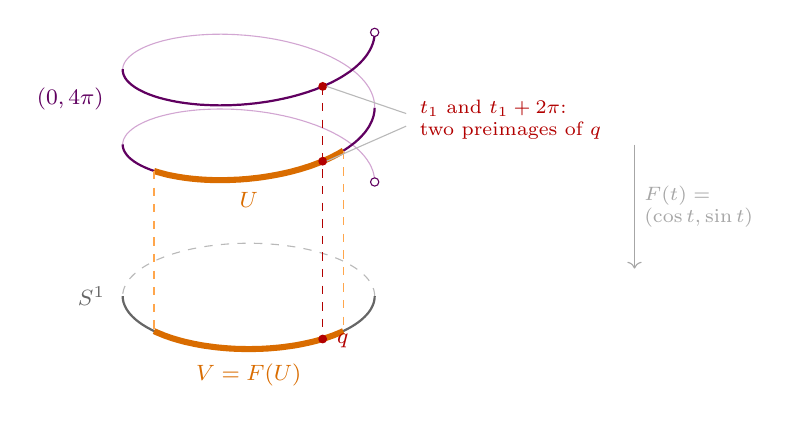
\begin{tikzpicture}
\draw[gray!55,dashed] (1.600,0.000) -- (1.599,0.027) -- (1.595,0.053) -- (1.589,0.080) -- (1.580,0.106) -- (1.568,0.133) -- (1.555,0.159) -- (1.538,0.185) -- (1.520,0.210) -- (1.499,0.235) -- (1.475,0.260) -- (1.449,0.285) -- (1.421,0.309) -- (1.391,0.332) -- (1.358,0.355) -- (1.324,0.377) -- (1.287,0.399) -- (1.248,0.420) -- (1.207,0.441) -- (1.165,0.461) -- (1.120,0.480) -- (1.074,0.498) -- (1.026,0.516) -- (0.976,0.532) -- (0.925,0.548) -- (0.872,0.563) -- (0.818,0.577) -- (0.763,0.591) -- (0.706,0.603) -- (0.649,0.614) -- (0.590,0.625) -- (0.531,0.634) -- (0.470,0.642) -- (0.409,0.650) -- (0.347,0.656) -- (0.285,0.661) -- (0.222,0.666) -- (0.159,0.669) -- (0.095,0.671) -- (0.032,0.672) -- (-0.032,0.672) -- (-0.095,0.671) -- (-0.159,0.669) -- (-0.222,0.666) -- (-0.285,0.661) -- (-0.347,0.656) -- (-0.409,0.650) -- (-0.470,0.642) -- (-0.531,0.634) -- (-0.590,0.625) -- (-0.649,0.614) -- (-0.706,0.603) -- (-0.763,0.591) -- (-0.818,0.577) -- (-0.872,0.563) -- (-0.925,0.548) -- (-0.976,0.532) -- (-1.026,0.516) -- (-1.074,0.498) -- (-1.120,0.480) -- (-1.165,0.461) -- (-1.207,0.441) -- (-1.248,0.420) -- (-1.287,0.399) -- (-1.324,0.377) -- (-1.358,0.355) -- (-1.391,0.332) -- (-1.421,0.309) -- (-1.449,0.285) -- (-1.475,0.260) -- (-1.499,0.235) -- (-1.520,0.210) -- (-1.538,0.185) -- (-1.555,0.159) -- (-1.568,0.133) -- (-1.580,0.106) -- (-1.589,0.080) -- (-1.595,0.053) -- (-1.599,0.027) -- (-1.600,0.000);
\draw[gray!80!black,thick] (-1.600,0.000) -- (-1.599,-0.027) -- (-1.595,-0.053) -- (-1.589,-0.080) -- (-1.580,-0.106) -- (-1.568,-0.133) -- (-1.555,-0.159) -- (-1.538,-0.185) -- (-1.520,-0.210) -- (-1.499,-0.235) -- (-1.475,-0.260) -- (-1.449,-0.285) -- (-1.421,-0.309) -- (-1.391,-0.332) -- (-1.358,-0.355) -- (-1.324,-0.377) -- (-1.287,-0.399) -- (-1.248,-0.420) -- (-1.207,-0.441) -- (-1.165,-0.461) -- (-1.120,-0.480) -- (-1.074,-0.498) -- (-1.026,-0.516) -- (-0.976,-0.532) -- (-0.925,-0.548) -- (-0.872,-0.563) -- (-0.818,-0.577) -- (-0.763,-0.591) -- (-0.706,-0.603) -- (-0.649,-0.614) -- (-0.590,-0.625) -- (-0.531,-0.634) -- (-0.470,-0.642) -- (-0.409,-0.650) -- (-0.347,-0.656) -- (-0.285,-0.661) -- (-0.222,-0.666) -- (-0.159,-0.669) -- (-0.095,-0.671) -- (-0.032,-0.672) -- (0.032,-0.672) -- (0.095,-0.671) -- (0.159,-0.669) -- (0.222,-0.666) -- (0.285,-0.661) -- (0.347,-0.656) -- (0.409,-0.650) -- (0.470,-0.642) -- (0.531,-0.634) -- (0.590,-0.625) -- (0.649,-0.614) -- (0.706,-0.603) -- (0.763,-0.591) -- (0.818,-0.577) -- (0.872,-0.563) -- (0.925,-0.548) -- (0.976,-0.532) -- (1.026,-0.516) -- (1.074,-0.498) -- (1.120,-0.480) -- (1.165,-0.461) -- (1.207,-0.441) -- (1.248,-0.420) -- (1.287,-0.399) -- (1.324,-0.377) -- (1.358,-0.355) -- (1.391,-0.332) -- (1.421,-0.309) -- (1.449,-0.285) -- (1.475,-0.260) -- (1.499,-0.235) -- (1.520,-0.210) -- (1.538,-0.185) -- (1.555,-0.159) -- (1.568,-0.133) -- (1.580,-0.106) -- (1.589,-0.080) -- (1.595,-0.053) -- (1.599,-0.027) -- (1.600,-0.000);
\draw[violet!35] (1.600,1.466) -- (1.599,1.481) -- (1.598,1.496) -- (1.596,1.511) -- (1.593,1.525) -- (1.590,1.540) -- (1.587,1.555) -- (1.583,1.569) -- (1.579,1.584) -- (1.574,1.599) -- (1.568,1.613) -- (1.562,1.628) -- (1.556,1.642) -- (1.549,1.656) -- (1.542,1.671) -- (1.534,1.685) -- (1.525,1.699) -- (1.516,1.713) -- (1.507,1.728) -- (1.497,1.742) -- (1.487,1.755) -- (1.476,1.769) -- (1.465,1.783) -- (1.453,1.797) -- (1.441,1.810) -- (1.428,1.824) -- (1.415,1.837) -- (1.401,1.851) -- (1.387,1.864) -- (1.373,1.877) -- (1.358,1.890) -- (1.342,1.903) -- (1.326,1.916) -- (1.310,1.928) -- (1.294,1.941) -- (1.276,1.953) -- (1.259,1.965) -- (1.241,1.977) -- (1.223,1.989) -- (1.204,2.001) -- (1.185,2.013) -- (1.166,2.024) -- (1.146,2.036) -- (1.125,2.047) -- (1.105,2.058) -- (1.084,2.069) -- (1.063,2.080) -- (1.041,2.091) -- (1.019,2.101) -- (0.997,2.111) -- (0.974,2.122) -- (0.951,2.131) -- (0.928,2.141) -- (0.905,2.151) -- (0.881,2.160) -- (0.857,2.170) -- (0.833,2.179) -- (0.808,2.187) -- (0.783,2.196) -- (0.758,2.205) -- (0.733,2.213) -- (0.707,2.221) -- (0.681,2.229) -- (0.655,2.237) -- (0.629,2.244) -- (0.602,2.252) -- (0.576,2.259) -- (0.549,2.266) -- (0.522,2.273) -- (0.495,2.279) -- (0.467,2.285) -- (0.440,2.292) -- (0.412,2.297) -- (0.384,2.303) -- (0.356,2.309) -- (0.328,2.314) -- (0.300,2.319) -- (0.272,2.324) -- (0.244,2.329) -- (0.215,2.333) -- (0.187,2.337) -- (0.159,2.341) -- (0.130,2.345) -- (0.101,2.349) -- (0.073,2.352) -- (0.044,2.355) -- (0.015,2.358) -- (-0.013,2.361) -- (-0.042,2.363) -- (-0.071,2.366) -- (-0.099,2.368) -- (-0.128,2.369) -- (-0.156,2.371) -- (-0.185,2.373) -- (-0.213,2.374) -- (-0.242,2.375) -- (-0.270,2.376) -- (-0.298,2.376) -- (-0.326,2.376) -- (-0.354,2.377) -- (-0.382,2.377) -- (-0.410,2.376) -- (-0.438,2.376) -- (-0.465,2.375) -- (-0.493,2.374) -- (-0.520,2.373) -- (-0.547,2.372) -- (-0.574,2.370) -- (-0.600,2.369) -- (-0.627,2.367) -- (-0.653,2.365) -- (-0.679,2.362) -- (-0.705,2.360) -- (-0.731,2.357) -- (-0.756,2.354) -- (-0.781,2.351) -- (-0.806,2.348) -- (-0.831,2.344) -- (-0.855,2.341) -- (-0.879,2.337) -- (-0.903,2.333) -- (-0.926,2.329) -- (-0.950,2.324) -- (-0.973,2.320) -- (-0.995,2.315) -- (-1.018,2.310) -- (-1.040,2.305) -- (-1.061,2.300) -- (-1.082,2.295) -- (-1.103,2.289) -- (-1.124,2.284) -- (-1.144,2.278) -- (-1.164,2.272) -- (-1.184,2.266) -- (-1.203,2.259) -- (-1.221,2.253) -- (-1.240,2.246) -- (-1.258,2.240) -- (-1.275,2.233) -- (-1.292,2.226) -- (-1.309,2.219) -- (-1.325,2.212) -- (-1.341,2.204) -- (-1.356,2.197) -- (-1.371,2.189) -- (-1.386,2.182) -- (-1.400,2.174) -- (-1.414,2.166) -- (-1.427,2.158) -- (-1.440,2.150) -- (-1.452,2.142) -- (-1.464,2.133) -- (-1.475,2.125) -- (-1.486,2.117) -- (-1.496,2.108) -- (-1.506,2.100) -- (-1.516,2.091) -- (-1.525,2.082) -- (-1.533,2.073) -- (-1.541,2.065) -- (-1.549,2.056) -- (-1.555,2.047) -- (-1.562,2.038) -- (-1.568,2.029) -- (-1.573,2.019) -- (-1.578,2.010) -- (-1.583,2.001) -- (-1.587,1.992) -- (-1.590,1.983) -- (-1.593,1.973) -- (-1.595,1.964) -- (-1.597,1.955) -- (-1.599,1.945) -- (-1.600,1.936) -- (-1.600,1.927);
\draw[violet!75!black,thick] (-1.600,1.927) -- (-1.600,1.917) -- (-1.599,1.908) -- (-1.598,1.899) -- (-1.596,1.889) -- (-1.594,1.880) -- (-1.591,1.871) -- (-1.588,1.862) -- (-1.584,1.852) -- (-1.580,1.843) -- (-1.575,1.834) -- (-1.570,1.825) -- (-1.564,1.816) -- (-1.558,1.807) -- (-1.551,1.798) -- (-1.544,1.789) -- (-1.536,1.780) -- (-1.528,1.771) -- (-1.519,1.762) -- (-1.510,1.754) -- (-1.500,1.745) -- (-1.490,1.737) -- (-1.479,1.728) -- (-1.468,1.720) -- (-1.457,1.711) -- (-1.444,1.703) -- (-1.432,1.695) -- (-1.419,1.687) -- (-1.405,1.679) -- (-1.391,1.671) -- (-1.377,1.664) -- (-1.362,1.656) -- (-1.347,1.649) -- (-1.331,1.641) -- (-1.315,1.634) -- (-1.299,1.627) -- (-1.282,1.620) -- (-1.264,1.613) -- (-1.247,1.606) -- (-1.228,1.600) -- (-1.210,1.593) -- (-1.191,1.587) -- (-1.172,1.581) -- (-1.152,1.575) -- (-1.132,1.569) -- (-1.111,1.563) -- (-1.091,1.557) -- (-1.069,1.552) -- (-1.048,1.547) -- (-1.026,1.542) -- (-1.004,1.537) -- (-0.981,1.532) -- (-0.959,1.527) -- (-0.935,1.523) -- (-0.912,1.519) -- (-0.888,1.515) -- (-0.864,1.511) -- (-0.840,1.507) -- (-0.816,1.503) -- (-0.791,1.500) -- (-0.766,1.497) -- (-0.740,1.494) -- (-0.715,1.491) -- (-0.689,1.489) -- (-0.663,1.486) -- (-0.637,1.484) -- (-0.611,1.482) -- (-0.584,1.480) -- (-0.557,1.479) -- (-0.530,1.477) -- (-0.503,1.476) -- (-0.476,1.475) -- (-0.448,1.474) -- (-0.421,1.474) -- (-0.393,1.474) -- (-0.365,1.473) -- (-0.337,1.473) -- (-0.309,1.474) -- (-0.281,1.474) -- (-0.253,1.475) -- (-0.224,1.476) -- (-0.196,1.477) -- (-0.167,1.478) -- (-0.139,1.480) -- (-0.110,1.482) -- (-0.082,1.484) -- (-0.053,1.486) -- (-0.024,1.488) -- (0.004,1.491) -- (0.033,1.494) -- (0.062,1.497) -- (0.090,1.500) -- (0.119,1.504) -- (0.148,1.507) -- (0.176,1.511) -- (0.205,1.515) -- (0.233,1.520) -- (0.261,1.524) -- (0.290,1.529) -- (0.318,1.534) -- (0.346,1.539) -- (0.374,1.545) -- (0.401,1.550) -- (0.429,1.556) -- (0.457,1.562) -- (0.484,1.568) -- (0.511,1.575) -- (0.538,1.582) -- (0.565,1.588) -- (0.592,1.596) -- (0.619,1.603) -- (0.645,1.610) -- (0.671,1.618) -- (0.697,1.626) -- (0.723,1.634) -- (0.748,1.642) -- (0.773,1.651) -- (0.798,1.659) -- (0.823,1.668) -- (0.848,1.677) -- (0.872,1.686) -- (0.896,1.695) -- (0.919,1.705) -- (0.943,1.715) -- (0.966,1.725) -- (0.988,1.735) -- (1.011,1.745) -- (1.033,1.755) -- (1.055,1.766) -- (1.076,1.777) -- (1.097,1.788) -- (1.118,1.799) -- (1.138,1.810) -- (1.158,1.821) -- (1.178,1.833) -- (1.197,1.844) -- (1.216,1.856) -- (1.234,1.868) -- (1.252,1.880) -- (1.270,1.892) -- (1.287,1.905) -- (1.304,1.917) -- (1.320,1.930) -- (1.336,1.942) -- (1.352,1.955) -- (1.367,1.968) -- (1.382,1.981) -- (1.396,1.994) -- (1.410,2.008) -- (1.423,2.021) -- (1.436,2.034) -- (1.448,2.048) -- (1.460,2.062) -- (1.472,2.075) -- (1.483,2.089) -- (1.493,2.103) -- (1.503,2.117) -- (1.513,2.131) -- (1.522,2.145) -- (1.531,2.159) -- (1.539,2.174) -- (1.546,2.188) -- (1.553,2.202) -- (1.560,2.217) -- (1.566,2.231) -- (1.572,2.246) -- (1.577,2.260) -- (1.581,2.275) -- (1.586,2.290) -- (1.589,2.304) -- (1.592,2.319) -- (1.595,2.334) -- (1.597,2.348) -- (1.598,2.363) -- (1.599,2.378) -- (1.600,2.393);
\draw[violet!35] (1.600,2.393) -- (1.600,2.407) -- (1.599,2.422) -- (1.598,2.437) -- (1.597,2.452) -- (1.595,2.466) -- (1.592,2.481) -- (1.589,2.496) -- (1.586,2.510) -- (1.581,2.525) -- (1.577,2.540) -- (1.572,2.554) -- (1.566,2.569) -- (1.560,2.583) -- (1.553,2.598) -- (1.546,2.612) -- (1.539,2.626) -- (1.531,2.641) -- (1.522,2.655) -- (1.513,2.669) -- (1.503,2.683) -- (1.493,2.697) -- (1.483,2.711) -- (1.472,2.725) -- (1.460,2.738) -- (1.448,2.752) -- (1.436,2.766) -- (1.423,2.779) -- (1.410,2.792) -- (1.396,2.806) -- (1.382,2.819) -- (1.367,2.832) -- (1.352,2.845) -- (1.336,2.858) -- (1.320,2.870) -- (1.304,2.883) -- (1.287,2.895) -- (1.270,2.908) -- (1.252,2.920) -- (1.234,2.932) -- (1.216,2.944) -- (1.197,2.956) -- (1.178,2.967) -- (1.158,2.979) -- (1.138,2.990) -- (1.118,3.001) -- (1.097,3.012) -- (1.076,3.023) -- (1.055,3.034) -- (1.033,3.045) -- (1.011,3.055) -- (0.988,3.065) -- (0.966,3.075) -- (0.943,3.085) -- (0.919,3.095) -- (0.896,3.105) -- (0.872,3.114) -- (0.848,3.123) -- (0.823,3.132) -- (0.798,3.141) -- (0.773,3.149) -- (0.748,3.158) -- (0.723,3.166) -- (0.697,3.174) -- (0.671,3.182) -- (0.645,3.190) -- (0.619,3.197) -- (0.592,3.204) -- (0.565,3.212) -- (0.538,3.218) -- (0.511,3.225) -- (0.484,3.232) -- (0.457,3.238) -- (0.429,3.244) -- (0.401,3.250) -- (0.374,3.255) -- (0.346,3.261) -- (0.318,3.266) -- (0.290,3.271) -- (0.261,3.276) -- (0.233,3.280) -- (0.205,3.285) -- (0.176,3.289) -- (0.148,3.293) -- (0.119,3.296) -- (0.090,3.300) -- (0.062,3.303) -- (0.033,3.306) -- (0.004,3.309) -- (-0.024,3.312) -- (-0.053,3.314) -- (-0.082,3.316) -- (-0.110,3.318) -- (-0.139,3.320) -- (-0.167,3.322) -- (-0.196,3.323) -- (-0.224,3.324) -- (-0.253,3.325) -- (-0.281,3.326) -- (-0.309,3.326) -- (-0.337,3.327) -- (-0.365,3.327) -- (-0.393,3.326) -- (-0.421,3.326) -- (-0.448,3.326) -- (-0.476,3.325) -- (-0.503,3.324) -- (-0.530,3.323) -- (-0.557,3.321) -- (-0.584,3.320) -- (-0.611,3.318) -- (-0.637,3.316) -- (-0.663,3.314) -- (-0.689,3.311) -- (-0.715,3.309) -- (-0.740,3.306) -- (-0.766,3.303) -- (-0.791,3.300) -- (-0.816,3.297) -- (-0.840,3.293) -- (-0.864,3.289) -- (-0.888,3.285) -- (-0.912,3.281) -- (-0.935,3.277) -- (-0.959,3.273) -- (-0.981,3.268) -- (-1.004,3.263) -- (-1.026,3.258) -- (-1.048,3.253) -- (-1.069,3.248) -- (-1.091,3.243) -- (-1.111,3.237) -- (-1.132,3.231) -- (-1.152,3.225) -- (-1.172,3.219) -- (-1.191,3.213) -- (-1.210,3.207) -- (-1.228,3.200) -- (-1.247,3.194) -- (-1.264,3.187) -- (-1.282,3.180) -- (-1.299,3.173) -- (-1.315,3.166) -- (-1.331,3.159) -- (-1.347,3.151) -- (-1.362,3.144) -- (-1.377,3.136) -- (-1.391,3.129) -- (-1.405,3.121) -- (-1.419,3.113) -- (-1.432,3.105) -- (-1.444,3.097) -- (-1.457,3.089) -- (-1.468,3.080) -- (-1.479,3.072) -- (-1.490,3.063) -- (-1.500,3.055) -- (-1.510,3.046) -- (-1.519,3.038) -- (-1.528,3.029) -- (-1.536,3.020) -- (-1.544,3.011) -- (-1.551,3.002) -- (-1.558,2.993) -- (-1.564,2.984) -- (-1.570,2.975) -- (-1.575,2.966) -- (-1.580,2.957) -- (-1.584,2.948) -- (-1.588,2.938) -- (-1.591,2.929) -- (-1.594,2.920) -- (-1.596,2.911) -- (-1.598,2.901) -- (-1.599,2.892) -- (-1.600,2.883);
\draw[violet!75!black,thick] (-1.600,2.883) -- (-1.600,2.873) -- (-1.600,2.864) -- (-1.599,2.855) -- (-1.597,2.845) -- (-1.595,2.836) -- (-1.593,2.827) -- (-1.590,2.817) -- (-1.587,2.808) -- (-1.583,2.799) -- (-1.578,2.790) -- (-1.573,2.781) -- (-1.568,2.771) -- (-1.562,2.762) -- (-1.555,2.753) -- (-1.549,2.744) -- (-1.541,2.735) -- (-1.533,2.727) -- (-1.525,2.718) -- (-1.516,2.709) -- (-1.506,2.700) -- (-1.496,2.692) -- (-1.486,2.683) -- (-1.475,2.675) -- (-1.464,2.667) -- (-1.452,2.658) -- (-1.440,2.650) -- (-1.427,2.642) -- (-1.414,2.634) -- (-1.400,2.626) -- (-1.386,2.618) -- (-1.371,2.611) -- (-1.356,2.603) -- (-1.341,2.596) -- (-1.325,2.588) -- (-1.309,2.581) -- (-1.292,2.574) -- (-1.275,2.567) -- (-1.258,2.560) -- (-1.240,2.554) -- (-1.221,2.547) -- (-1.203,2.541) -- (-1.184,2.534) -- (-1.164,2.528) -- (-1.144,2.522) -- (-1.124,2.516) -- (-1.103,2.511) -- (-1.082,2.505) -- (-1.061,2.500) -- (-1.040,2.495) -- (-1.018,2.490) -- (-0.995,2.485) -- (-0.973,2.480) -- (-0.950,2.476) -- (-0.926,2.471) -- (-0.903,2.467) -- (-0.879,2.463) -- (-0.855,2.459) -- (-0.831,2.456) -- (-0.806,2.452) -- (-0.781,2.449) -- (-0.756,2.446) -- (-0.731,2.443) -- (-0.705,2.440) -- (-0.679,2.438) -- (-0.653,2.435) -- (-0.627,2.433) -- (-0.600,2.431) -- (-0.574,2.430) -- (-0.547,2.428) -- (-0.520,2.427) -- (-0.493,2.426) -- (-0.465,2.425) -- (-0.438,2.424) -- (-0.410,2.424) -- (-0.382,2.423) -- (-0.354,2.423) -- (-0.326,2.424) -- (-0.298,2.424) -- (-0.270,2.424) -- (-0.242,2.425) -- (-0.213,2.426) -- (-0.185,2.427) -- (-0.156,2.429) -- (-0.128,2.431) -- (-0.099,2.432) -- (-0.071,2.434) -- (-0.042,2.437) -- (-0.013,2.439) -- (0.015,2.442) -- (0.044,2.445) -- (0.073,2.448) -- (0.101,2.451) -- (0.130,2.455) -- (0.159,2.459) -- (0.187,2.463) -- (0.215,2.467) -- (0.244,2.471) -- (0.272,2.476) -- (0.300,2.481) -- (0.328,2.486) -- (0.356,2.491) -- (0.384,2.497) -- (0.412,2.503) -- (0.440,2.508) -- (0.467,2.515) -- (0.495,2.521) -- (0.522,2.527) -- (0.549,2.534) -- (0.576,2.541) -- (0.602,2.548) -- (0.629,2.556) -- (0.655,2.563) -- (0.681,2.571) -- (0.707,2.579) -- (0.733,2.587) -- (0.758,2.595) -- (0.783,2.604) -- (0.808,2.613) -- (0.833,2.621) -- (0.857,2.630) -- (0.881,2.640) -- (0.905,2.649) -- (0.928,2.659) -- (0.951,2.669) -- (0.974,2.678) -- (0.997,2.689) -- (1.019,2.699) -- (1.041,2.709) -- (1.063,2.720) -- (1.084,2.731) -- (1.105,2.742) -- (1.125,2.753) -- (1.146,2.764) -- (1.166,2.776) -- (1.185,2.787) -- (1.204,2.799) -- (1.223,2.811) -- (1.241,2.823) -- (1.259,2.835) -- (1.276,2.847) -- (1.294,2.859) -- (1.310,2.872) -- (1.326,2.884) -- (1.342,2.897) -- (1.358,2.910) -- (1.373,2.923) -- (1.387,2.936) -- (1.401,2.949) -- (1.415,2.963) -- (1.428,2.976) -- (1.441,2.990) -- (1.453,3.003) -- (1.465,3.017) -- (1.476,3.031) -- (1.487,3.045) -- (1.497,3.058) -- (1.507,3.072) -- (1.516,3.087) -- (1.525,3.101) -- (1.534,3.115) -- (1.542,3.129) -- (1.549,3.144) -- (1.556,3.158) -- (1.562,3.172) -- (1.568,3.187) -- (1.574,3.201) -- (1.579,3.216) -- (1.583,3.231) -- (1.587,3.245) -- (1.590,3.260) -- (1.593,3.275) -- (1.596,3.289) -- (1.598,3.304) -- (1.599,3.319) -- (1.600,3.334);
\draw[violet!75!black,fill=white] (1.600,1.450) circle (1.5pt);
\draw[violet!75!black,fill=white] (1.600,3.350) circle (1.5pt);
\draw[orange!85!black,line width=2.2pt] (-1.202,1.590) -- (-1.171,1.580) -- (-1.139,1.571) -- (-1.106,1.562) -- (-1.073,1.553) -- (-1.038,1.544) -- (-1.002,1.536) -- (-0.966,1.529) -- (-0.929,1.522) -- (-0.891,1.515) -- (-0.852,1.509) -- (-0.813,1.503) -- (-0.773,1.498) -- (-0.732,1.493) -- (-0.691,1.489) -- (-0.649,1.485) -- (-0.607,1.482) -- (-0.564,1.479) -- (-0.521,1.477) -- (-0.477,1.475) -- (-0.433,1.474) -- (-0.388,1.474) -- (-0.343,1.473) -- (-0.298,1.474) -- (-0.252,1.475) -- (-0.207,1.477) -- (-0.161,1.479) -- (-0.115,1.481) -- (-0.069,1.485) -- (-0.023,1.488) -- (0.023,1.493) -- (0.069,1.498) -- (0.115,1.503) -- (0.161,1.509) -- (0.207,1.516) -- (0.252,1.523) -- (0.298,1.531) -- (0.343,1.539) -- (0.388,1.548) -- (0.433,1.557) -- (0.477,1.567) -- (0.521,1.577) -- (0.564,1.588) -- (0.607,1.600) -- (0.649,1.611) -- (0.691,1.624) -- (0.732,1.637) -- (0.773,1.650) -- (0.813,1.664) -- (0.852,1.679) -- (0.891,1.694) -- (0.929,1.709) -- (0.966,1.725) -- (1.002,1.741) -- (1.038,1.758) -- (1.073,1.775) -- (1.106,1.793) -- (1.139,1.810) -- (1.171,1.829) -- (1.202,1.848);
\draw[orange!85!black,line width=2.2pt] (-1.202,-0.444) -- (-1.171,-0.458) -- (-1.139,-0.472) -- (-1.106,-0.485) -- (-1.073,-0.499) -- (-1.038,-0.511) -- (-1.002,-0.524) -- (-0.966,-0.536) -- (-0.929,-0.547) -- (-0.891,-0.558) -- (-0.852,-0.569) -- (-0.813,-0.579) -- (-0.773,-0.588) -- (-0.732,-0.597) -- (-0.691,-0.606) -- (-0.649,-0.614) -- (-0.607,-0.622) -- (-0.564,-0.629) -- (-0.521,-0.635) -- (-0.477,-0.641) -- (-0.433,-0.647) -- (-0.388,-0.652) -- (-0.343,-0.656) -- (-0.298,-0.660) -- (-0.252,-0.664) -- (-0.207,-0.666) -- (-0.161,-0.669) -- (-0.115,-0.670) -- (-0.069,-0.671) -- (-0.023,-0.672) -- (0.023,-0.672) -- (0.069,-0.671) -- (0.115,-0.670) -- (0.161,-0.669) -- (0.207,-0.666) -- (0.252,-0.664) -- (0.298,-0.660) -- (0.343,-0.656) -- (0.388,-0.652) -- (0.433,-0.647) -- (0.477,-0.641) -- (0.521,-0.635) -- (0.564,-0.629) -- (0.607,-0.622) -- (0.649,-0.614) -- (0.691,-0.606) -- (0.732,-0.597) -- (0.773,-0.588) -- (0.813,-0.579) -- (0.852,-0.569) -- (0.891,-0.558) -- (0.929,-0.547) -- (0.966,-0.536) -- (1.002,-0.524) -- (1.038,-0.511) -- (1.073,-0.499) -- (1.106,-0.485) -- (1.139,-0.472) -- (1.171,-0.458) -- (1.202,-0.444);
\draw[orange!70,dashed,thin] (-1.202,1.590) -- (-1.202,-0.444);
\draw[orange!70,dashed,thin] (1.202,1.848) -- (1.202,-0.444);
\node[orange!85!black,font=\footnotesize,anchor=north] at (-0.000,1.440) {$U$};
\node[orange!85!black,font=\footnotesize,anchor=north] at (-0.000,-0.732) {$V = F(U)$};
\draw[red!70!black,dashed] (0.940,2.664) -- (0.940,-0.544);
\fill[red!70!black] (0.940,1.714) circle (1.6pt);
\fill[red!70!black] (0.940,2.664) circle (1.6pt);
\fill[red!70!black] (0.940,-0.544) circle (1.6pt);
\node[red!70!black,font=\footnotesize,anchor=west] at (1.000,-0.564) {$q$};
\draw[gray!55,thin] (0.990,1.714) -- (2.000,2.159);
\draw[gray!55,thin] (0.990,2.664) -- (2.000,2.319);
\node[red!70!black,font=\scriptsize,anchor=west,align=left] at (2.050,2.239) {$t_1$ and $t_1 + 2\pi$:\\ two preimages of $q$};
\node[violet!75!black,font=\footnotesize,anchor=east] at (-1.720,2.500) {$(0,4\pi)$};
\node[gray!80!black,font=\footnotesize,anchor=east] at (-1.700,0.000) {$S^1$};
\draw[->,gray!70] (4.900,1.925) -- node[right,font=\scriptsize,align=left]{$F(t) =$\\$(\cos t, \sin t)$} (4.900,0.350);
\end{tikzpicture}
\end{center}

The helix is the interval $(0, 4\pi)$, lifted so that $F$ becomes the vertical projection onto the circle. On the orange interval $U$ the projection is a diffeomorphism onto the arc $V$; but the point $q \in V$ has a second preimage $t_1 + 2\pi$, on the other turn and outside $U$. Local invertibility does not see it.


The projection $S^n \to \mathbb{RP}^n$, a two-to-one local diffeomorphism, is collected in Section~\ref{sec:ex-hopf}.


\begin{rembox}[Covering Maps]\label{rem:covering-maps}
Uribe noted that $\mathbb{R} \to S^1$ and $S^n \to \mathbb{RP}^n$ are \emph{covering maps}, while $(0, 4\pi) \to S^1$ is a local diffeomorphism that is not: over the point $F(0) = (1,0)$ it has a single preimage, $2\pi$, where every other point of the circle has two. Covering maps were not defined in lecture and the distinction was postponed (``we're running a little bit behind schedule''); it is Lee Ch.\ 4.
\end{rembox}

The converse direction of the main theorem rests on one theorem from analysis --- ``that's really what's paying the bills here.''

\begin{thmbox}[Inverse Function Theorem]\thmlabel{thm:inverse-function}
Let $W \subseteq \mathbb{R}^n$ be open, $\Phi : W \to \mathbb{R}^n$ smooth, and $a \in W$ with $\Phi'(a)$ invertible. Then there are open sets $U_0 \ni a$ in $W$ and $V_0 \ni \Phi(a)$ in $\mathbb{R}^n$ such that $\Phi(U_0) = V_0$ and $\Phi|_{U_0} : U_0 \to V_0$ is bijective with smooth inverse.
\leeref{Theorem C.34}
\end{thmbox}

\begin{proof}[Proof (to be filled)]
Taken from analysis, not proved in this course (Lee, Theorem~C.34; MATH~452 proves the two-variable case). To be filled.
\end{proof}

Lee, Theorem C.34; taken from analysis, not proved in the course. It should not be confused with the \emph{implicit} function theorem of \S\ref{sub:ift} --- the board's ``IFT'' now means the inverse one. Each theorem can be derived from the other.

\begin{thmbox}[Local Diffeomorphisms Are Detected by the Differential]\thmlabel{thm:local-diffeo-criterion}
A smooth map $F : M \to N$ is a local diffeomorphism if and only if $F_{*p} : T_pM \to T_{F(p)}N$ is bijective for every $p \in M$.
\leeref{Theorem 4.5 and Proposition 4.8}
\end{thmbox}

\begin{proof}
\textit{(Lecture~10. The forward direction was supplied by a student at Uribe's prompting --- use the local inverse and the chain rule; for the converse the inverse function theorem ``is really what's paying the bills here.'' The identification of $(F|_U^V)_{*p}$ with $F_{*p}$ is a completion.)} ($\Rightarrow$) Let $G : V \to U$ be a local inverse at $p$, so that $G \circ F|_U^V = \mathrm{id}_U$ and $F|_U^V \circ G = \mathrm{id}_V$. By the Chain Rule (Theorem~\ref{prop:pushforward-functorial}),
\[
G_{*F(p)} \circ (F|_U^V)_{*p} = \mathrm{id}, \qquad (F|_U^V)_{*p} \circ G_{*F(p)} = \mathrm{id},
\]
so $(F|_U^V)_{*p}$ is bijective with inverse $G_{*F(p)}$. Under the identifications $T_pU = T_pM$ and $T_{F(p)}V = T_{F(p)}N$ of Lemma~\ref{lem:germs-local}, $(F|_U^V)_{*p}$ is $F_{*p}$, again by the Chain Rule applied to $F \circ \iota_U = \iota_V \circ F|_U^V$.

($\Leftarrow$) Fix $p$, and choose charts $(U,\varphi)$ at $p$ and $(V,\psi)$ at $F(p)$ with $F(U) \subseteq V$. A bijective linear map forces $\dim M = \dim N$, and by Theorem~\ref{lem:differential-matrix} the matrix of $F_{*p}$ is the square matrix $\tilde F'(\varphi(p))$; so the latter is invertible. By the Inverse Function Theorem there are open sets $\tilde A \ni \varphi(p)$ in $\varphi(U)$ and $\tilde B \ni \tilde F(\varphi(p))$ such that $\tilde F|_{\tilde A} : \tilde A \to \tilde B$ is bijective with smooth inverse. Put $U' = \varphi^{-1}(\tilde A)$ and $V' = \psi^{-1}(\tilde B)$, neighbourhoods of $p$ and $F(p)$; since $\varphi$ is a homeomorphism, ``shrinking $\varphi(U)$ is the same as shrinking $U$.'' On $U'$ we have $F = \psi^{-1} \circ \tilde F \circ \varphi$, so $F(U') = V'$ and
\[
\big(F|_{U'}^{V'}\big)^{-1} = \varphi^{-1} \circ \big(\tilde F|_{\tilde A}\big)^{-1} \circ \psi|_{V'},
\]
a composite of diffeomorphisms (Proposition~\ref{prop:chart-diffeo}), hence smooth.
\end{proof}

\begin{center}
\begin{tikzcd}[row sep=3.2em, column sep=5em]
U' \arrow[r, shift left=0.8ex, "F|_{U'}^{V'}"] \arrow[d, "\varphi"', "\cong"] & V' \arrow[l, shift left=0.8ex, "G"] \arrow[d, "\psi", "\cong"'] \\
\tilde A \arrow[r, shift left=0.8ex, "\tilde F"] & \tilde B \arrow[l, shift left=0.8ex, "\tilde F^{-1}"]
\end{tikzcd}
\end{center}

The converse in one picture. Downstairs the Inverse Function Theorem supplies $\tilde F^{-1}$; the charts carry it upstairs as the local inverse $G = \varphi^{-1} \circ \tilde F^{-1} \circ \psi$. The only input from the hypothesis is that the bottom arrow has an invertible Jacobian at $\varphi(p)$ --- which is where Theorem~\ref{lem:differential-matrix} enters.

A student asked why $\tilde F'(\varphi(p))$ is invertible; Uribe's answer was the lemma just cited: the Jacobian \emph{is} the matrix of $F_{*p}$ in coordinate bases, and $F_{*p}$ is bijective by hypothesis. The practical content of the theorem is that ``being a local diffeomorphism is detectable'' by computing one Jacobian at each point, rather than by exhibiting local inverses.

\begin{corbox}[Diffeomorphisms Are the Bijective Local Diffeomorphisms]\thmlabel{cor:bijective-local-diffeo}
A smooth map $F : M \to N$ is a diffeomorphism if and only if it is a bijective local diffeomorphism. Consequently, a smooth bijection with $F_{*p}$ bijective at every $p \in M$ is a diffeomorphism.
\leeref{Proposition 4.6}
\end{corbox}

\begin{proof}
A diffeomorphism is a local diffeomorphism with $U = M$ and $V = N$. Conversely, let $F$ be a bijective local diffeomorphism. Given $q \in N$, let $p = F^{-1}(q)$ and let $G : V \to U$ be a local inverse at $p$. For $y \in V$, $G(y) \in U$ and $F(G(y)) = y$, so $G(y) = F^{-1}(y)$ because $F$ is injective. Thus $F^{-1}$ agrees on the open neighbourhood $V$ of $q$ with the smooth map $G$. As $q$ was arbitrary, $F^{-1}$ is continuous and smooth, since both properties are local. The last sentence follows from Theorem~\ref{thm:local-diffeo-criterion}.
\end{proof}

\begin{rembox}\label{rem:special-maps-2}
Not stated in lecture. Injectivity is the entire difference between the two notions, as the helix of Example~\ref{ex:line-circle} shows: there every local inverse exists, but they cannot be assembled into a global one, because the second preimage of $q$ lies outside the domain of the local inverse. The same argument shows that a bijective local homeomorphism is a homeomorphism.
\end{rembox}

% ============================================================================
% SECTION: SUBMERSIONS
% ============================================================================

\section{Submersions}\label{sec:submersions}\label{sub:submersions}

\roadmark{Stage: maps}{Maps with surjective differentials: locally projections, by the normal form --- the tool that makes the regular value theorem work on any manifold (\ref{sec:submanifolds}).}

\begin{defbox}[Submersion and Immersion]\deflabel{def:submersion}
Let $F : M \to N$ be smooth and $p \in M$. $F$ is a \textbf{submersion at $p$} if $F_{*p}$ is onto, and a \textbf{submersion} if it is a submersion at every point. $F$ is an \textbf{immersion at $p$} if $F_{*p}$ is injective, and an \textbf{immersion} if it is one at every point.
\leeref{Ch.~4, \emph{Maps of Constant Rank}}
\end{defbox}

The submersion half is the lecture's definition. Immersions were listed as the third special type and treated in Lecture~13 (\ref{sub:immersions}); the definition is recorded here in Lee's form so that the three types can be compared. In the language of Definition~\ref{def:manifold-regular}, $F$ is a submersion at $p$ exactly when $p$ is a regular point.

\begin{propbox}[Dimension Constraints]\thmlabel{prop:dimension-constraints}
Let $F : M \to N$ be smooth, $m = \dim M$, $n = \dim N$, and $p \in M$.
\begin{enumerate}
    \item If $F$ is a submersion at $p$ then $n \le m$; if $F$ is an immersion at $p$ then $m \le n$.
    \item $F$ is a local diffeomorphism if and only if it is both a submersion and an immersion; in that case $m = n$.
    \item If $m = n$ and $F$ is a submersion, or an immersion, at every point, then $F$ is a local diffeomorphism.
\end{enumerate}
\leeref{Proposition 4.8}
\end{propbox}

\begin{proof}
(1) By rank--nullity (Proposition~\ref{fact:linalg}(1)), a surjective linear map $T_pM \to T_{F(p)}N$ forces $n \le m$, and an injective one forces $m \le n$. (2) A linear map is bijective if and only if it is injective and surjective, so this is Theorem~\ref{thm:local-diffeo-criterion}; then (1) gives $m = n$. (3) Between spaces of the same finite dimension, a linear map is injective iff surjective iff bijective (Proposition~\ref{fact:linalg}(1)); apply Theorem~\ref{thm:local-diffeo-criterion}.
\end{proof}

\begin{exbox}[Projections Are Submersions]\exlabel{ex:projection-submersion}
The projection $\pi : \mathbb{R}^k \times \mathbb{R}^l \to \mathbb{R}^k$, $(x, y) \mapsto x$, is a submersion.
\end{exbox}

\begin{proof}
By Proposition~\ref{prop:differential-agree} the differential is the Jacobian $\big(I_k \mid 0\big)$, a $k \times (k+l)$ matrix of rank $k$.
\end{proof}

\textbf{Transcription note.} Page 28 of the handwritten notes writes the projection as $\mathbb{R}^m \times \mathbb{R}^l \to \mathbb{R}^k$; for a projection onto a factor the factor must be the target, $\mathbb{R}^k \times \mathbb{R}^l \to \mathbb{R}^k$. Projections of \emph{product manifolds} $M_1 \times M_2 \to M_1$ are submersions for the same reason, but that needs the tangent space of a product --- ``they will be direct sums of tangent spaces'' --- which Uribe postponed to the next lecture.

Lecture~11 supplied it (Theorem~\ref{thm:tangent-product}):

\begin{exbox}[Projections of Product Manifolds Are Submersions]\exlabel{ex:product-projection-submersion}
The projection $\pi_1 : M_1 \times M_2 \to M_1$ is a submersion, and so is $\pi_2$.
\leeref{Proposition 3.14}
\end{exbox}

\begin{proof}
$\pi_{1*}\big(\Theta(v, w)\big) = \pi_{1*}\iota_{1*}v + \pi_{1*}\iota_{2*}w = v$, by the proof of Theorem~\ref{thm:tangent-product}; so $\pi_{1*}$ is onto $T_{p_1}M_1$.
\end{proof}

The projection $S^{2n+1} \to \mathbb{CP}^n$, a submersion, is collected in Section~\ref{sec:ex-hopf}.

\begin{defbox}[Regular Points and Critical Points]\deflabel{def:regular-critical}
Let $F : M \to N$ be smooth, with $\dim M = m$ and $\dim N = n$.
\begin{enumerate}
    \item $p \in M$ is a \textbf{regular point} of $F$ if $F$ is a submersion at $p$, i.e.\ $F_{*p}$ is onto --- which forces $n \le m$. Otherwise $p$ is a \textbf{critical point}, also called a \textbf{singular point}.
    \item $q \in N$ is a \textbf{regular value} of $F$ if $F$ is a submersion at every $p \in F^{-1}(q)$, and a \textbf{critical value} otherwise.
    \item In particular every $q \notin F(M)$ is a regular value: its preimage is empty, and ``everything is true for the empty set.''
\end{enumerate}
These are the notions of Definition~\ref{def:manifold-regular}, now with critical points and the empty-preimage convention made explicit; for maps between open subsets of Euclidean spaces they are those of Definition~\ref{def:regular-value}.
\end{defbox}

Uribe called (3) ``kind of a trivial way to be [regular], but important'': it matters in Sard's theorem, about the set of regular values, which is still to come. \textbf{Transcription note.} Page 29 of the handwritten notes has ``if $q \in \operatorname{Im} F$, then $q$ is regular''; the audio has ``if $q$ is not in the image of $F$'', as in (3). The same page writes the preimage in (2) as $F^{-1}(p)$ for $F^{-1}(q)$.

\begin{propbox}[Critical Points of Real-Valued Functions]\thmlabel{prop:critical-functions}
Let $f : M \to \mathbb{R}$ be smooth. Then $df_p$ is either onto or zero, so
\[
p \text{ is a critical point of } f \iff df_p = 0 \iff \frac{\partial f}{\partial x^i}(p) = 0 \text{ for all } i,
\]
in any chart at $p$.
\leeref{Exercise 11.24}
\end{propbox}

\begin{proof}
The image of the linear map $df_p$ is a subspace of the one-dimensional $T_{f(p)}\mathbb{R} \cong \mathbb{R}$ (Definition~\ref{def:cotangent}), so it is $0$ or everything --- ``dimensions of images cannot be fractional.'' The second equivalence is Lemma~\ref{lem:df-coords}.
\end{proof}

This is the definition of critical point Uribe sent to the class by email, and it agrees with Definition~\ref{def:regular-value} for $m = 1$: there $p$ is regular iff $\nabla F(p) \ne 0$.

\begin{lembox}[Diffeomorphisms onto Open Sets Are Charts]\thmlabel{lem:diffeo-chart}
Let $U \subseteq M$ be open and $\hat\varphi : U \to \mathbb{R}^m$ smooth, with $\hat\varphi(U)$ open and $\hat\varphi : U \to \hat\varphi(U)$ a diffeomorphism. Then $(U, \hat\varphi)$ is a smooth chart of $M$.
\leeref{cf.\ Ch.~2, \emph{Diffeomorphisms}}
\end{lembox}

\begin{proof}
It is a homeomorphism onto an open subset of $\mathbb{R}^m$, so it is a chart. For any smooth chart $(W, \chi)$ of $M$, the transition maps $\hat\varphi \circ \chi^{-1}$ and $\chi \circ \hat\varphi^{-1}$ are coordinate representations of $\hat\varphi$ and $\hat\varphi^{-1}$, smooth because these maps are (Proposition~\ref{prop:smooth-map-charts}). So $(U, \hat\varphi)$ is compatible with every chart of the maximal atlas, and therefore belongs to it (Theorem~\ref{thm:maximal-atlas}).
\end{proof}
\begin{thmbox}[Local Normal Form for Submersions]\thmlabel{thm:submersion-normal-form}
Let $F : M \to N$ be a submersion at $p$, with $\dim M = m$ and $\dim N = n$. Then there are charts $(U, \varphi)$ at $p$ and $(V, \psi)$ at $F(p)$ with $F(U) \subseteq V$ in which the coordinate representation $\tilde F = \psi \circ F \circ \varphi^{-1} : \varphi(U) \to \psi(V)$ is the projection onto the first $n$ coordinates:
\[
\tilde F\big(r^1, \ldots, r^m\big) = \big(r^1, \ldots, r^n\big).
\]
Equivalently, with coordinate functions $x^i = r^i \circ \varphi$ on $U$ and $y^j = r^j \circ \psi$ on $V$: $\;y^j \circ F = x^j$ on $U$ for $j = 1, \ldots, n$. In particular $n \le m$.
\leeref{Theorem 4.12, the rank theorem}
\end{thmbox}

Stated in Lecture 10 and proved in Lecture 11, below. The inequality $n \le m$ needs no theorem --- a surjective linear map cannot raise dimension --- but the normal form does: it says that every submersion, in suitable coordinates, \emph{is} a projection.

\begin{center}
\begin{tikzcd}[row sep=3em, column sep=11em]
U \arrow[r, "F"] \arrow[d, "\varphi"'] & V \arrow[d, "\psi"] \\
\varphi(U) \arrow[r, "{(r^1, \ldots, r^m) \,\mapsto\, (r^1, \ldots, r^n)}"'] & \psi(V)
\end{tikzcd}
\end{center}

\begin{center}
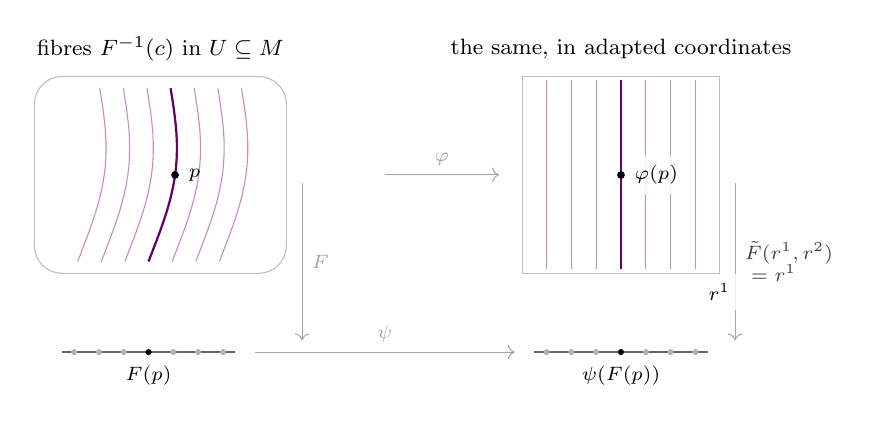
\begin{tikzpicture}
\begin{scope}
\draw[gray!50,rounded corners=10pt] (-1.45,-0.15) rectangle (1.75,2.35);
\draw[violet!45] (-0.900,0.000) -- (-0.889,0.028) -- (-0.879,0.056) -- (-0.868,0.084) -- (-0.857,0.111) -- (-0.847,0.139) -- (-0.836,0.167) -- (-0.825,0.195) -- (-0.815,0.223) -- (-0.804,0.251) -- (-0.793,0.278) -- (-0.783,0.306) -- (-0.773,0.334) -- (-0.762,0.362) -- (-0.752,0.390) -- (-0.742,0.418) -- (-0.732,0.446) -- (-0.722,0.473) -- (-0.713,0.501) -- (-0.703,0.529) -- (-0.694,0.557) -- (-0.685,0.585) -- (-0.676,0.613) -- (-0.667,0.641) -- (-0.659,0.668) -- (-0.651,0.696) -- (-0.643,0.724) -- (-0.635,0.752) -- (-0.628,0.780) -- (-0.620,0.808) -- (-0.614,0.835) -- (-0.607,0.863) -- (-0.601,0.891) -- (-0.595,0.919) -- (-0.589,0.947) -- (-0.583,0.975) -- (-0.578,1.003) -- (-0.574,1.030) -- (-0.569,1.058) -- (-0.565,1.086) -- (-0.561,1.114) -- (-0.558,1.142) -- (-0.554,1.170) -- (-0.551,1.197) -- (-0.549,1.225) -- (-0.547,1.253) -- (-0.545,1.281) -- (-0.543,1.309) -- (-0.542,1.337) -- (-0.541,1.365) -- (-0.540,1.392) -- (-0.540,1.420) -- (-0.540,1.448) -- (-0.540,1.476) -- (-0.540,1.504) -- (-0.541,1.532) -- (-0.542,1.559) -- (-0.544,1.587) -- (-0.545,1.615) -- (-0.547,1.643) -- (-0.549,1.671) -- (-0.551,1.699) -- (-0.554,1.727) -- (-0.557,1.754) -- (-0.560,1.782) -- (-0.563,1.810) -- (-0.566,1.838) -- (-0.570,1.866) -- (-0.573,1.894) -- (-0.577,1.922) -- (-0.581,1.949) -- (-0.585,1.977) -- (-0.589,2.005) -- (-0.593,2.033) -- (-0.598,2.061) -- (-0.602,2.089) -- (-0.606,2.116) -- (-0.611,2.144) -- (-0.615,2.172) -- (-0.620,2.200);
\draw[violet!45] (-0.600,0.000) -- (-0.589,0.028) -- (-0.579,0.056) -- (-0.568,0.084) -- (-0.557,0.111) -- (-0.547,0.139) -- (-0.536,0.167) -- (-0.525,0.195) -- (-0.515,0.223) -- (-0.504,0.251) -- (-0.493,0.278) -- (-0.483,0.306) -- (-0.473,0.334) -- (-0.462,0.362) -- (-0.452,0.390) -- (-0.442,0.418) -- (-0.432,0.446) -- (-0.422,0.473) -- (-0.413,0.501) -- (-0.403,0.529) -- (-0.394,0.557) -- (-0.385,0.585) -- (-0.376,0.613) -- (-0.367,0.641) -- (-0.359,0.668) -- (-0.351,0.696) -- (-0.343,0.724) -- (-0.335,0.752) -- (-0.328,0.780) -- (-0.320,0.808) -- (-0.314,0.835) -- (-0.307,0.863) -- (-0.301,0.891) -- (-0.295,0.919) -- (-0.289,0.947) -- (-0.283,0.975) -- (-0.278,1.003) -- (-0.274,1.030) -- (-0.269,1.058) -- (-0.265,1.086) -- (-0.261,1.114) -- (-0.258,1.142) -- (-0.254,1.170) -- (-0.251,1.197) -- (-0.249,1.225) -- (-0.247,1.253) -- (-0.245,1.281) -- (-0.243,1.309) -- (-0.242,1.337) -- (-0.241,1.365) -- (-0.240,1.392) -- (-0.240,1.420) -- (-0.240,1.448) -- (-0.240,1.476) -- (-0.240,1.504) -- (-0.241,1.532) -- (-0.242,1.559) -- (-0.244,1.587) -- (-0.245,1.615) -- (-0.247,1.643) -- (-0.249,1.671) -- (-0.251,1.699) -- (-0.254,1.727) -- (-0.257,1.754) -- (-0.260,1.782) -- (-0.263,1.810) -- (-0.266,1.838) -- (-0.270,1.866) -- (-0.273,1.894) -- (-0.277,1.922) -- (-0.281,1.949) -- (-0.285,1.977) -- (-0.289,2.005) -- (-0.293,2.033) -- (-0.298,2.061) -- (-0.302,2.089) -- (-0.306,2.116) -- (-0.311,2.144) -- (-0.315,2.172) -- (-0.320,2.200);
\draw[violet!45] (-0.300,0.000) -- (-0.289,0.028) -- (-0.279,0.056) -- (-0.268,0.084) -- (-0.257,0.111) -- (-0.247,0.139) -- (-0.236,0.167) -- (-0.225,0.195) -- (-0.215,0.223) -- (-0.204,0.251) -- (-0.193,0.278) -- (-0.183,0.306) -- (-0.173,0.334) -- (-0.162,0.362) -- (-0.152,0.390) -- (-0.142,0.418) -- (-0.132,0.446) -- (-0.122,0.473) -- (-0.113,0.501) -- (-0.103,0.529) -- (-0.094,0.557) -- (-0.085,0.585) -- (-0.076,0.613) -- (-0.067,0.641) -- (-0.059,0.668) -- (-0.051,0.696) -- (-0.043,0.724) -- (-0.035,0.752) -- (-0.028,0.780) -- (-0.020,0.808) -- (-0.014,0.835) -- (-0.007,0.863) -- (-0.001,0.891) -- (0.005,0.919) -- (0.011,0.947) -- (0.017,0.975) -- (0.022,1.003) -- (0.026,1.030) -- (0.031,1.058) -- (0.035,1.086) -- (0.039,1.114) -- (0.042,1.142) -- (0.046,1.170) -- (0.049,1.197) -- (0.051,1.225) -- (0.053,1.253) -- (0.055,1.281) -- (0.057,1.309) -- (0.058,1.337) -- (0.059,1.365) -- (0.060,1.392) -- (0.060,1.420) -- (0.060,1.448) -- (0.060,1.476) -- (0.060,1.504) -- (0.059,1.532) -- (0.058,1.559) -- (0.056,1.587) -- (0.055,1.615) -- (0.053,1.643) -- (0.051,1.671) -- (0.049,1.699) -- (0.046,1.727) -- (0.043,1.754) -- (0.040,1.782) -- (0.037,1.810) -- (0.034,1.838) -- (0.030,1.866) -- (0.027,1.894) -- (0.023,1.922) -- (0.019,1.949) -- (0.015,1.977) -- (0.011,2.005) -- (0.007,2.033) -- (0.002,2.061) -- (-0.002,2.089) -- (-0.006,2.116) -- (-0.011,2.144) -- (-0.015,2.172) -- (-0.020,2.200);
\draw[violet!75!black,thick] (-0.000,0.000) -- (0.011,0.028) -- (0.021,0.056) -- (0.032,0.084) -- (0.043,0.111) -- (0.053,0.139) -- (0.064,0.167) -- (0.075,0.195) -- (0.085,0.223) -- (0.096,0.251) -- (0.107,0.278) -- (0.117,0.306) -- (0.127,0.334) -- (0.138,0.362) -- (0.148,0.390) -- (0.158,0.418) -- (0.168,0.446) -- (0.178,0.473) -- (0.187,0.501) -- (0.197,0.529) -- (0.206,0.557) -- (0.215,0.585) -- (0.224,0.613) -- (0.233,0.641) -- (0.241,0.668) -- (0.249,0.696) -- (0.257,0.724) -- (0.265,0.752) -- (0.272,0.780) -- (0.280,0.808) -- (0.286,0.835) -- (0.293,0.863) -- (0.299,0.891) -- (0.305,0.919) -- (0.311,0.947) -- (0.317,0.975) -- (0.322,1.003) -- (0.326,1.030) -- (0.331,1.058) -- (0.335,1.086) -- (0.339,1.114) -- (0.342,1.142) -- (0.346,1.170) -- (0.349,1.197) -- (0.351,1.225) -- (0.353,1.253) -- (0.355,1.281) -- (0.357,1.309) -- (0.358,1.337) -- (0.359,1.365) -- (0.360,1.392) -- (0.360,1.420) -- (0.360,1.448) -- (0.360,1.476) -- (0.360,1.504) -- (0.359,1.532) -- (0.358,1.559) -- (0.356,1.587) -- (0.355,1.615) -- (0.353,1.643) -- (0.351,1.671) -- (0.349,1.699) -- (0.346,1.727) -- (0.343,1.754) -- (0.340,1.782) -- (0.337,1.810) -- (0.334,1.838) -- (0.330,1.866) -- (0.327,1.894) -- (0.323,1.922) -- (0.319,1.949) -- (0.315,1.977) -- (0.311,2.005) -- (0.307,2.033) -- (0.302,2.061) -- (0.298,2.089) -- (0.294,2.116) -- (0.289,2.144) -- (0.285,2.172) -- (0.280,2.200);
\draw[violet!45] (0.300,0.000) -- (0.311,0.028) -- (0.321,0.056) -- (0.332,0.084) -- (0.343,0.111) -- (0.353,0.139) -- (0.364,0.167) -- (0.375,0.195) -- (0.385,0.223) -- (0.396,0.251) -- (0.407,0.278) -- (0.417,0.306) -- (0.427,0.334) -- (0.438,0.362) -- (0.448,0.390) -- (0.458,0.418) -- (0.468,0.446) -- (0.478,0.473) -- (0.487,0.501) -- (0.497,0.529) -- (0.506,0.557) -- (0.515,0.585) -- (0.524,0.613) -- (0.533,0.641) -- (0.541,0.668) -- (0.549,0.696) -- (0.557,0.724) -- (0.565,0.752) -- (0.572,0.780) -- (0.580,0.808) -- (0.586,0.835) -- (0.593,0.863) -- (0.599,0.891) -- (0.605,0.919) -- (0.611,0.947) -- (0.617,0.975) -- (0.622,1.003) -- (0.626,1.030) -- (0.631,1.058) -- (0.635,1.086) -- (0.639,1.114) -- (0.642,1.142) -- (0.646,1.170) -- (0.649,1.197) -- (0.651,1.225) -- (0.653,1.253) -- (0.655,1.281) -- (0.657,1.309) -- (0.658,1.337) -- (0.659,1.365) -- (0.660,1.392) -- (0.660,1.420) -- (0.660,1.448) -- (0.660,1.476) -- (0.660,1.504) -- (0.659,1.532) -- (0.658,1.559) -- (0.656,1.587) -- (0.655,1.615) -- (0.653,1.643) -- (0.651,1.671) -- (0.649,1.699) -- (0.646,1.727) -- (0.643,1.754) -- (0.640,1.782) -- (0.637,1.810) -- (0.634,1.838) -- (0.630,1.866) -- (0.627,1.894) -- (0.623,1.922) -- (0.619,1.949) -- (0.615,1.977) -- (0.611,2.005) -- (0.607,2.033) -- (0.602,2.061) -- (0.598,2.089) -- (0.594,2.116) -- (0.589,2.144) -- (0.585,2.172) -- (0.580,2.200);
\draw[violet!45] (0.600,0.000) -- (0.611,0.028) -- (0.621,0.056) -- (0.632,0.084) -- (0.643,0.111) -- (0.653,0.139) -- (0.664,0.167) -- (0.675,0.195) -- (0.685,0.223) -- (0.696,0.251) -- (0.707,0.278) -- (0.717,0.306) -- (0.727,0.334) -- (0.738,0.362) -- (0.748,0.390) -- (0.758,0.418) -- (0.768,0.446) -- (0.778,0.473) -- (0.787,0.501) -- (0.797,0.529) -- (0.806,0.557) -- (0.815,0.585) -- (0.824,0.613) -- (0.833,0.641) -- (0.841,0.668) -- (0.849,0.696) -- (0.857,0.724) -- (0.865,0.752) -- (0.872,0.780) -- (0.880,0.808) -- (0.886,0.835) -- (0.893,0.863) -- (0.899,0.891) -- (0.905,0.919) -- (0.911,0.947) -- (0.917,0.975) -- (0.922,1.003) -- (0.926,1.030) -- (0.931,1.058) -- (0.935,1.086) -- (0.939,1.114) -- (0.942,1.142) -- (0.946,1.170) -- (0.949,1.197) -- (0.951,1.225) -- (0.953,1.253) -- (0.955,1.281) -- (0.957,1.309) -- (0.958,1.337) -- (0.959,1.365) -- (0.960,1.392) -- (0.960,1.420) -- (0.960,1.448) -- (0.960,1.476) -- (0.960,1.504) -- (0.959,1.532) -- (0.958,1.559) -- (0.956,1.587) -- (0.955,1.615) -- (0.953,1.643) -- (0.951,1.671) -- (0.949,1.699) -- (0.946,1.727) -- (0.943,1.754) -- (0.940,1.782) -- (0.937,1.810) -- (0.934,1.838) -- (0.930,1.866) -- (0.927,1.894) -- (0.923,1.922) -- (0.919,1.949) -- (0.915,1.977) -- (0.911,2.005) -- (0.907,2.033) -- (0.902,2.061) -- (0.898,2.089) -- (0.894,2.116) -- (0.889,2.144) -- (0.885,2.172) -- (0.880,2.200);
\draw[violet!45] (0.900,0.000) -- (0.911,0.028) -- (0.921,0.056) -- (0.932,0.084) -- (0.943,0.111) -- (0.953,0.139) -- (0.964,0.167) -- (0.975,0.195) -- (0.985,0.223) -- (0.996,0.251) -- (1.007,0.278) -- (1.017,0.306) -- (1.027,0.334) -- (1.038,0.362) -- (1.048,0.390) -- (1.058,0.418) -- (1.068,0.446) -- (1.078,0.473) -- (1.087,0.501) -- (1.097,0.529) -- (1.106,0.557) -- (1.115,0.585) -- (1.124,0.613) -- (1.133,0.641) -- (1.141,0.668) -- (1.149,0.696) -- (1.157,0.724) -- (1.165,0.752) -- (1.172,0.780) -- (1.180,0.808) -- (1.186,0.835) -- (1.193,0.863) -- (1.199,0.891) -- (1.205,0.919) -- (1.211,0.947) -- (1.217,0.975) -- (1.222,1.003) -- (1.226,1.030) -- (1.231,1.058) -- (1.235,1.086) -- (1.239,1.114) -- (1.242,1.142) -- (1.246,1.170) -- (1.249,1.197) -- (1.251,1.225) -- (1.253,1.253) -- (1.255,1.281) -- (1.257,1.309) -- (1.258,1.337) -- (1.259,1.365) -- (1.260,1.392) -- (1.260,1.420) -- (1.260,1.448) -- (1.260,1.476) -- (1.260,1.504) -- (1.259,1.532) -- (1.258,1.559) -- (1.256,1.587) -- (1.255,1.615) -- (1.253,1.643) -- (1.251,1.671) -- (1.249,1.699) -- (1.246,1.727) -- (1.243,1.754) -- (1.240,1.782) -- (1.237,1.810) -- (1.234,1.838) -- (1.230,1.866) -- (1.227,1.894) -- (1.223,1.922) -- (1.219,1.949) -- (1.215,1.977) -- (1.211,2.005) -- (1.207,2.033) -- (1.202,2.061) -- (1.198,2.089) -- (1.194,2.116) -- (1.189,2.144) -- (1.185,2.172) -- (1.180,2.200);
\fill (0.337,1.100) circle (1.4pt); \node[font=\scriptsize,anchor=west] at (0.387,1.100) {$p$};
\draw[gray!80!black,thick] (-1.1,-1.15) -- (1.1,-1.15);
\fill[gray!60] (-0.945,-1.15) circle (1.1pt);
\fill[gray!60] (-0.630,-1.15) circle (1.1pt);
\fill[gray!60] (-0.315,-1.15) circle (1.1pt);
\fill[black] (-0.000,-1.15) circle (1.1pt);
\fill[gray!60] (0.315,-1.15) circle (1.1pt);
\fill[gray!60] (0.630,-1.15) circle (1.1pt);
\fill[gray!60] (0.945,-1.15) circle (1.1pt);
\node[font=\scriptsize,anchor=north] at (0,-1.2) {$F(p)$};
\draw[->,gray!70] (1.95,1.0) -- node[right,font=\scriptsize]{$F$} (1.95,-1.0);
\node[font=\footnotesize] at (0.15,2.7) {fibres $F^{-1}(c)$ in $U \subseteq M$};
\end{scope}
\begin{scope}[xshift=6.0cm]
\draw[gray!50] (-1.25,-0.15) rectangle (1.25,2.35);
\draw[violet!45] (-0.945,-0.1) -- (-0.945,2.3);
\draw[violet!45] (-0.630,-0.1) -- (-0.630,2.3);
\draw[violet!45] (-0.315,-0.1) -- (-0.315,2.3);
\draw[violet!75!black,thick] (-0.000,-0.1) -- (-0.000,2.3);
\draw[violet!45] (0.315,-0.1) -- (0.315,2.3);
\draw[violet!45] (0.630,-0.1) -- (0.630,2.3);
\draw[violet!45] (0.945,-0.1) -- (0.945,2.3);
\fill (0,1.1) circle (1.4pt); \node[fill=white, fill opacity=0.85, text opacity=1, font=\scriptsize,anchor=west] at (0.05,1.1) {$\varphi(p)$};
\draw[gray!80!black,thick] (-1.1,-1.15) -- (1.1,-1.15);
\fill[gray!60] (-0.945,-1.15) circle (1.1pt);
\fill[gray!60] (-0.630,-1.15) circle (1.1pt);
\fill[gray!60] (-0.315,-1.15) circle (1.1pt);
\fill[black] (-0.000,-1.15) circle (1.1pt);
\fill[gray!60] (0.315,-1.15) circle (1.1pt);
\fill[gray!60] (0.630,-1.15) circle (1.1pt);
\fill[gray!60] (0.945,-1.15) circle (1.1pt);
\node[font=\scriptsize,anchor=north] at (0,-1.2) {$\psi(F(p))$};
\draw[->,gray!70] (1.45,1.0) -- node[right,font=\scriptsize,align=left,text=black!75]{$\tilde F(r^1,r^2)$\\$\;= r^1$} (1.45,-1.0);
\node[fill=white, fill opacity=0.85, text opacity=1, font=\scriptsize,anchor=north] at (1.25,-0.15) {$r^1$};
\node[font=\footnotesize] at (0,2.7) {the same, in adapted coordinates};
\end{scope}
\draw[->,gray!70] (3.0,1.1) -- node[above,font=\scriptsize]{$\varphi$} (4.45,1.1);
\draw[->,gray!70] (1.35,-1.15) -- node[above,font=\scriptsize]{$\psi$} (4.65,-1.15);
\end{tikzpicture}
\end{center}

What the normal form says, for $m = 2$ and $n = 1$. Left: near $p$ the fibres $F^{-1}(c)$ of a submersion are curves, one through each point, which $F$ collapses to the points of an interval. Right: in the charts of the theorem the fibres are straightened into vertical lines, and $\tilde F$ forgets the second coordinate. Every submersion looks, locally and up to a change of coordinates, like the projection of Example~\ref{ex:projection-submersion}.

% ============================================================
% Lecture 11 (Fri Sep 25, 2026)
% ============================================================

\textit{Lecture 11. ``Back to submersions.'' Uribe now made the vocabulary official, with the letters matched to the dimensions: $\dim M = m$ and $\dim N = n$. (In \ref{sec:rvt}, following the earlier lecture, $F : \mathbb{R}^N \to \mathbb{R}^m$ had $m$ as the dimension of the target.)}


Uribe singled out Lemma~\ref{lem:diffeo-chart} as ``an intellectual step that should not be overlooked'': in the proof below, a map is shown to be a local diffeomorphism, and this lemma is what makes it a coordinate system.

\begin{proof}[Proof (Lecture 11)]
The steps are the lecture's, in the lecture's order. Sentences marked \textit{(Completion.)} fill in details the lecture passed over.

\emph{1. Start with any coordinates.} ``I start with any coordinates'': smooth charts $(U_0, \varphi_0 = (x^1, \ldots, x^m))$ at $p$ and $(V, \psi = (y^1, \ldots, y^n))$ at $F(p)$ with $F(U_0) \subseteq V$. \textit{(Completion.)} Such charts exist: take any charts and replace $U_0$ by the open set $U_0 \cap F^{-1}(V)$.

\emph{2. The components and their matrix.} As before, define the components of $F$, $F^j = y^j \circ F : U_0 \to \mathbb{R}$. The submersion condition says that the matrix
\[
J = \Big[\frac{\partial F^j}{\partial x^i}(p)\Big]
\]
has rank $n$. It ``has $m$ columns, which are the $x$'s, and $n$ rows, that are the gradients'' of the $F^j$. \textit{(Completion.)} By Theorem~\ref{lem:differential-matrix}, $J$ is the matrix of $F_{*p}$ in the coordinate bases, and $F_{*p}$ is onto, so $J$ has rank $n$.

\emph{3. ``It's the same matrix.''} A student asked whether the matrix should be written with $\tilde F$. Uribe: ``It's the same thing\ldots\ That's how we define partials. We define them by going downstairs and taking the ordinary partial derivative downstairs. So it's the same matrix.'' That is Proposition~\ref{prop:upstairs-downstairs}: writing $G = \psi \circ F \circ \varphi_0^{-1}$ for the coordinate representation in these first charts (the lecture's $\tilde F$ at this stage),
\[
\frac{\partial F^j}{\partial x^i}(p) = \frac{\partial G^j}{\partial r^i}\big(\varphi_0(p)\big), \qquad J = G'\big(\varphi_0(p)\big).
\]

\emph{4. Reindex --- ``the only thing we need to do.''} $J$ has $n$ linearly independent columns; ``I just put them at the beginning.'' Rearranging the $x^i$, we can write $J$ in block form
\[
J = \big(\, A \ \big|\ B \,\big), \qquad A \text{ an } n \times n \text{ non-singular matrix}, \quad B \text{ of size } n \times (m - n),
\]
where $B$ is ``the stuff that remains here that I'm not going to care about.'' \textit{(Completion.)} Rearranging the coordinates replaces $\varphi_0$ by $P \circ \varphi_0$ for a permutation $P$ of $\mathbb{R}^m$. This is again a smooth chart: a chart by Lemma~\ref{lem:chart-modify}, and its transition maps are those of $\varphi_0$ composed with the linear map $P$ or $P^{-1}$, hence smooth. It permutes the columns of $J$ in the same way.

\emph{5. The coordinates we want.} ``The thing to do, you see, is to take the first $n$ components of $F$ as the first $n$ coordinate functions, and then we keep the remaining ones'':
\[
\hat\varphi = \big(F^1, \ldots, F^n, x^{n+1}, \ldots, x^m\big) : U_0 \to \mathbb{R}^m .
\]
\textit{(Completion.)} This makes sense because $n \le m$ --- the theorem's ``in particular'', true since $F_{*p}$ is onto (Proposition~\ref{prop:dimension-constraints}) --- so there are $m - n \ge 0$ remaining coordinates. $\hat\varphi$ is smooth because its components are. It has $m$ components, so it maps into $\mathbb{R}^m$ (see the transcription note below).

\emph{6. The claim.} $\hat\varphi$ is a local diffeomorphism in a neighbourhood of $p$.

\emph{7. The Jacobian of $\hat\varphi$ in the old coordinates.} ``Gradient across'': the first $n$ rows are the gradients of $F^1, \ldots, F^n$, which give the matrix $J = (A \mid B)$; the last $m - n$ rows are the gradients of $x^{n+1}, \ldots, x^m$. These give the $(m-n) \times (m-n)$ identity, and zero in the first $n$ columns, ``because I would be taking partials of these $x$'s with respect to $x$'s that come before.'' So
\[
\begin{pmatrix} A & B \\ 0 & I_{m-n} \end{pmatrix},
\]
and ``by the block nature, the fact that we have a big zero there, this is non-degenerate'' at $p$: its determinant is $\det A \ne 0$. \textit{(Completion.)} ``The Jacobian of $\hat\varphi$ in the $x$-coordinates'' is the Jacobian at $\varphi_0(p)$ of the ordinary map $H = \hat\varphi \circ \varphi_0^{-1} : \varphi_0(U_0) \to \mathbb{R}^m$. Its rows are the partials of the components of $\hat\varphi$ by Proposition~\ref{prop:upstairs-downstairs}, applied with the identity chart on $\mathbb{R}^m$, and $\partial x^k/\partial x^i = \delta^k_i$ gives the identity and zero blocks.

\emph{8. The inverse function theorem, ``possibly after shrinking $U$.''} By the inverse function theorem (Theorem~\ref{thm:inverse-function}), possibly after shrinking, $\hat\varphi$ is a diffeomorphism onto $\hat\varphi(U)$. \textit{(Completion.)} The theorem gives an open $W \ni \varphi_0(p)$, contained in $\varphi_0(U_0)$, with $H|_W$ a diffeomorphism onto the open set $H(W) \subseteq \mathbb{R}^m$. Put $U = \varphi_0^{-1}(W)$, an open neighbourhood of $p$. Then $\hat\varphi|_U = H|_W \circ \varphi_0|_U$ is a composite of diffeomorphisms (Proposition~\ref{prop:chart-diffeo}, Lemma~\ref{lem:composition-smooth}), mapping $U$ onto the open set $\hat\varphi(U) = H(W)$.

\emph{9. The intellectual step: $\hat\varphi$ is a chart.} ``There's an intellectual step here that should not be overlooked. If I have a local diffeomorphism like this from an open set in $M$ into its image, which is open in $\mathbb{R}^m$, that is a chart'': it is a homeomorphism, and being smooth with smooth inverse makes it compatible with every other smooth chart, so it lies in the maximal atlas. This is Lemma~\ref{lem:diffeo-chart}. So $(U, \hat\varphi)$ is a smooth chart at $p$, and $F(U) \subseteq F(U_0) \subseteq V$.

\emph{10. Do not change the $y$-coordinates.} The chart $(V, \psi)$ on $N$ stays as it was. Only the chart on $M$ is new.

\emph{11. Going up and coming down.} Let $\tilde F = \psi \circ F \circ \hat\varphi^{-1} : \hat\varphi(U) \to \psi(V)$ be the coordinate representation of $F$ in the new chart. ``I take a point down here, $r^1$ up to $r^m$, and I go upstairs'': going up means finding the point $q = \hat\varphi^{-1}(r)$ of $U$ whose values of the first $n$ functions $F^1, \ldots, F^n$ are the first $n$ coordinates of $r$. By the definition of $\hat\varphi$,
\[
F^i\big(\hat\varphi^{-1}(r^1, \ldots, r^m)\big) = r^i \qquad (i = 1, \ldots, n).
\]
Coming back down by $\psi$, the $i$-th coordinate of $\tilde F(r)$ is $y^i(F(q)) = F^i(q) = r^i$. So $\tilde F(r^1, \ldots, r^m) = (r^1, \ldots, r^n)$: ``this coordinate system labels every point in $U$; the first $n$ labels are the values of the $F$'s at that point.''
\end{proof}

\begin{center}
\begin{tikzcd}[row sep=2.8em, column sep=3.8em]
& U \arrow[dl, "\varphi_0"'] \arrow[dr, "\hat\varphi"] \arrow[rr, "F"] & & V \arrow[d, "\psi"] \\
W \subseteq \varphi_0(U_0) \arrow[rr, "H = \hat\varphi \circ \varphi_0^{-1}"', "\cong"] & & \hat\varphi(U) \arrow[r, "\tilde F"'] & \psi(V)
\end{tikzcd}
\end{center}

The change of chart in one diagram. The first chart $\varphi_0$ and the new chart $\hat\varphi$ differ by $H$, a diffeomorphism near $\varphi_0(p)$ by step~8. In the new chart, $F$ becomes $\tilde F$, the projection (step~11). The lecture used the letters $\phi$ and $\tilde F$ both for the first charts and for the new ones. The notes write $\varphi_0$ and $G$ for the first, and $\hat\varphi$ and $\tilde F$ for the new, to keep the two stages apart.

\textbf{Transcription note.} In the lecture, $\hat\varphi$ was twice called ``a map from $U$ into $\mathbb{R}^n$'', and page 30 of the handwritten notes writes $\phi : U \to \mathbb{R}$; it has $m$ components, so $\hat\varphi : U \to \mathbb{R}^m$. The matrix of partials was spoken as ``$\partial x^j/\partial x^i$'', for $\partial F^j/\partial x^i$.

\begin{corbox}[Being a Submersion Is an Open Condition]\thmlabel{cor:submersion-open-condition}
If $F : M \to N$ is a submersion at $p$, then $F$ is a submersion at every point of some neighbourhood of $p$.
\leeref{Proposition 4.1}
\end{corbox}

\begin{proof}
In the charts of the theorem, $\tilde F$ is the projection, whose Jacobian $(I_n \mid 0)$ has rank $n$ at every point of $\hat\varphi(U)$. By Theorem~\ref{lem:differential-matrix}, $F_{*q}$ is onto for every $q \in U$.
\end{proof}

\begin{corbox}[Submersions Are Open Maps]\thmlabel{cor:submersion-open-map}
If $F : M \to N$ is a submersion, then $F(W)$ is open in $N$ for every open $W \subseteq M$.
\leeref{Proposition 4.28}
\end{corbox}

\begin{proof}
Let $q = F(p)$ with $p \in W$, and take the charts of the theorem at $p$, shrinking $U$ to $U \cap W$. Then $F(U) = \psi^{-1}\big(\mathrm{pr}(\hat\varphi(U))\big)$, where $\mathrm{pr} : \mathbb{R}^m \to \mathbb{R}^n$ is the projection onto the first $n$ coordinates. Projections are open (Example~\ref{ex:proj-open}), and $\hat\varphi(U)$ is open, so $\mathrm{pr}(\hat\varphi(U))$ is an open subset of $\psi(V)$, and $F(U)$ is open in $N$. It contains $q$ and lies in $F(W)$.
\end{proof}

\begin{thmbox}[Submersions from Compact Manifolds]\thmlabel{thm:compact-submersion}
Let $M$ be compact and nonempty, $N$ connected, and $F : M \to N$ a submersion. Then $F$ is surjective, and $N$ is compact.
\end{thmbox}

\begin{proof}
\textit{(Assignment~4, Problem~2, where $N = \mathbb{R}^k$; the same argument gives the general statement.)} $F(M)$ is open in $N$ because a submersion is an open map (Corollary~\ref{cor:submersion-open-map}), and compact, hence closed in the Hausdorff space $N$, because $M$ is compact. It is nonempty, and $N$ is connected, so $F(M) = N$. Then $N = F(M)$ is compact.
\end{proof}

\begin{corbox}[No Submersions from Compact Manifolds to Euclidean Space]\thmlabel{cor:no-submersion-Rk}
If $M$ is compact and nonempty and $k \ge 1$, there is no submersion $M \to \mathbb{R}^k$.
\end{corbox}

\begin{proof}
\textit{(Assignment~4, Problem~2.)} $\mathbb{R}^k$ is connected but not compact, since it is unbounded; apply Theorem~\ref{thm:compact-submersion}.
\end{proof}

The submitted solution also noted the edge cases: for $k = 0$ the constant map $M \to \mathbb{R}^0$ is a submersion, since every differential maps onto the zero space; and for $M = \emptyset$ the empty map is vacuously one. In particular, a compact manifold carries no nonconstant submersion to $\mathbb{R}$ --- the maximum of any smooth function $f : M \to \mathbb{R}$ is a critical point.

\section{Submanifolds}\label{sec:submanifolds-fibrations}\label{sec:submanifolds}

\roadmark{Stage: submanifolds}{Subsets of a manifold that are locally coordinate slices --- the equations thread, completed.}

\textit{References: Lee Ch.~5. Lecture 12.} The subsets of a manifold that look locally like $\mathbb{R}^{m-k} \subseteq \mathbb{R}^m$. The regular value theorem for manifolds, proved from the submersion normal form of \ref{sec:submersions}, produces them as level sets --- the end of the equations thread that began in \ref{sec:rvt}.

% ============================================================
% Lecture 12 (Mon Sep 28, 2026)
% ============================================================

\subsection{Submanifolds}\label{sub:submanifolds}

\textit{Lecture 12 (Mon Sep 28). ``I know we're in the middle of discussing submersions and fibrations, but we need the notion of submanifold. So let's pause to discuss that. It's not difficult.'' The local model is a lower-dimensional Euclidean space inside a higher-dimensional one: $\mathbb{R}^{m-k} \subseteq \mathbb{R}^m$ as the points whose last $k$ coordinates vanish, $x \mapsto (x, \vec 0)$.}

\begin{defbox}[Submanifold and Adapted Charts]\deflabel{def:submanifold}
Let $M$ be a smooth manifold of dimension $m$, $S \subseteq M$ a subset with the subspace topology, and $0 \le k \le m$. For a chart $\varphi = (x^1, \ldots, x^m)$ write $x_a = (x^1, \ldots, x^{m-k})$ for its first $m - k$ components and $x_b = (x^{m-k+1}, \ldots, x^m)$ for its last $k$. Then $S$ is a \textbf{submanifold of $M$ of codimension $k$} if every $p \in S$ lies in the domain of a smooth chart $(U, \varphi)$ of $M$ with
\[
U \cap S = \{\, q \in U : x_b(q) = \vec 0 \,\}.
\]
Such charts are \textbf{adapted} to $S$; ``a random chart of $M$ is not adapted.'' In an adapted chart, $U \cap S$ is cut out by the $k$ equations $x^{m-k+1} = \cdots = x^m = 0$, exactly as in the local model. These are sometimes called \textbf{regular} or \textbf{embedded} submanifolds, as opposed to the immersed submanifolds still to come.
\leeref{Theorem 5.8}
\end{defbox}

\begin{propbox}[Two Observations on Adapted Charts]\thmlabel{prop:adapted-flex}
Let $(U, \varphi)$ be a smooth chart of $M$, and suppose that $U \cap S$ is cut out in it by setting some $k$ of the coordinates equal to constants:
\[
U \cap S = \{\, q \in U : x^{i_1}(q) = c_1, \ \ldots, \ x^{i_k}(q) = c_k \,\}.
\]
Then there is an adapted chart with the same domain $U$. That is: (1) the value $\vec 0$ in the definition may be replaced by any constant vector $\vec c$, and (2) the last $k$ coordinates may be replaced by any $k$ of them.
\end{propbox}

\begin{proof}
\textit{(Lecture~12: ``obvious observations''; filled in.)} Let $P : \mathbb{R}^m \to \mathbb{R}^m$ be the permutation of coordinates that moves positions $i_1, \ldots, i_k$ to the last $k$ places, and $T(r) = r - (\vec 0, \vec c)$. Then $A = T \circ P$ is an affine diffeomorphism of $\mathbb{R}^m$, so $(U, A \circ \varphi)$ is a smooth chart: a chart by Lemma~\ref{lem:chart-modify}, whose transition maps with any smooth chart are those of $\varphi$ composed with $A$ or $A^{-1}$, hence smooth. Its last $k$ coordinates are $x^{i_1} - c_1, \ldots, x^{i_k} - c_k$, which vanish exactly on $U \cap S$.
\end{proof}

\begin{propbox}[The Induced Smooth Structure]\thmlabel{prop:submanifold-structure}
Let $S \subseteq M$ be a submanifold of codimension $k$. For each adapted chart $(U, \varphi = (x_a, x_b))$ put
\[
\varphi_S = x_a|_{U \cap S} : U \cap S \longrightarrow \mathbb{R}^{m-k}.
\]
Then (1) $U \cap S$ is open in $S$, and $\varphi_S$ is a homeomorphism onto an open subset of $\mathbb{R}^{m-k}$; and (2) the charts $(U \cap S, \varphi_S)$, over all adapted charts, form a smooth atlas $\mathcal{A}_S$ on $S$. So $S$ is a topological manifold of dimension $m - k$, and with the smooth structure generated by $\mathcal{A}_S$ it is a smooth manifold --- ``a manifold in its own right.''
\leeref{Theorem 5.8}
\end{propbox}

\begin{proof}
\textit{(Lecture~12 claimed (1) --- ``easy to check'' --- and gave the reason for (2); completed here.)} $S$ is Hausdorff and second countable as a subspace of $M$ (Theorem~\ref{thm:subspace-inherit}) --- ``back to week one of the class.'' Let $j : \mathbb{R}^{m-k} \to \mathbb{R}^m$, $j(r) = (r, \vec 0)$, and $\mathrm{pr} : \mathbb{R}^m \to \mathbb{R}^{m-k}$, $\mathrm{pr}(r, s) = r$.

(1) $U \cap S$ is open in $S$ by the definition of the subspace topology. Since $U \cap S = \{x_b = \vec 0\}$, the chart $\varphi$ maps $U \cap S$ bijectively onto $\varphi(U) \cap j(\mathbb{R}^{m-k}) = j(W)$, where $W = j^{-1}(\varphi(U))$ is open in $\mathbb{R}^{m-k}$ because $j$ is continuous. So $\varphi_S = \mathrm{pr} \circ \varphi|_{U \cap S}$ is a continuous bijection $U \cap S \to W$, with continuous inverse $r \mapsto \varphi^{-1}(j(r))$.

(2) Every point of $S$ lies in an adapted chart, so the domains cover $S$. For adapted charts $(U, \varphi)$ and $(V, \psi)$, since $\varphi_S^{-1} = \varphi^{-1} \circ j$,
\[
\psi_S \circ \varphi_S^{-1} = \mathrm{pr} \circ (\psi \circ \varphi^{-1}) \circ j \qquad \text{on } \varphi_S(U \cap V \cap S) = j^{-1}\big(\varphi(U \cap V)\big) .
\]
This is the transition map of $M$, which is smooth, composed with the linear maps $j$ and $\mathrm{pr}$: the transition maps of $S$ are ``restrictions to $\mathbb{R}^{m-k}$ of $C^\infty$ maps between open sets of $\mathbb{R}^m$.''
\end{proof}

\begin{center}
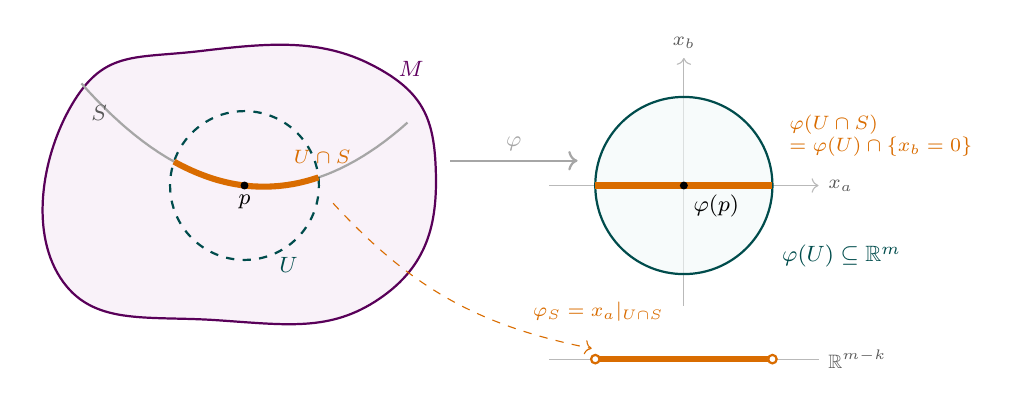
\begin{tikzpicture}[scale=0.9]
\draw[violet!70!black, thick, fill=violet!5] plot[smooth cycle, tension=0.8] coordinates {(-2.6,-1.3) (-2.4,1.2) (-0.6,1.9) (1.8,1.7) (2.7,0.2) (1.9,-1.6) (-0.4,-1.9)};
\node[violet!75!black, font=\footnotesize] at (2.35,1.65) {$M$};
\draw[gray!70, thick] (-2.300,1.440) -- (-2.261,1.396) -- (-2.223,1.354) -- (-2.184,1.311) -- (-2.145,1.270) -- (-2.107,1.229) -- (-2.068,1.189) -- (-2.029,1.150) -- (-1.991,1.111) -- (-1.952,1.073) -- (-1.913,1.035) -- (-1.875,0.998) -- (-1.836,0.962) -- (-1.797,0.927) -- (-1.759,0.892) -- (-1.720,0.857) -- (-1.682,0.824) -- (-1.643,0.791) -- (-1.604,0.759) -- (-1.566,0.727) -- (-1.527,0.696) -- (-1.488,0.666) -- (-1.450,0.636) -- (-1.411,0.607) -- (-1.372,0.579) -- (-1.334,0.551) -- (-1.295,0.524) -- (-1.256,0.498) -- (-1.218,0.472) -- (-1.179,0.447) -- (-1.140,0.423) -- (-1.102,0.399) -- (-1.063,0.376) -- (-1.024,0.354) -- (-0.986,0.332) -- (-0.947,0.311) -- (-0.908,0.291) -- (-0.870,0.271) -- (-0.831,0.252) -- (-0.792,0.233) -- (-0.754,0.215) -- (-0.715,0.198) -- (-0.676,0.182) -- (-0.638,0.166) -- (-0.599,0.151) -- (-0.561,0.136) -- (-0.522,0.123) -- (-0.483,0.109) -- (-0.445,0.097) -- (-0.406,0.085) -- (-0.367,0.074) -- (-0.329,0.063) -- (-0.290,0.053) -- (-0.251,0.044) -- (-0.213,0.035) -- (-0.174,0.028) -- (-0.135,0.020) -- (-0.097,0.014) -- (-0.058,0.008) -- (-0.019,0.002) -- (0.019,-0.002) -- (0.058,-0.006) -- (0.097,-0.010) -- (0.135,-0.012) -- (0.174,-0.014) -- (0.213,-0.016) -- (0.251,-0.016) -- (0.290,-0.016) -- (0.329,-0.016) -- (0.367,-0.014) -- (0.406,-0.012) -- (0.445,-0.010) -- (0.483,-0.007) -- (0.522,-0.003) -- (0.561,0.002) -- (0.599,0.007) -- (0.638,0.013) -- (0.676,0.019) -- (0.715,0.027) -- (0.754,0.035) -- (0.792,0.043) -- (0.831,0.052) -- (0.870,0.062) -- (0.908,0.073) -- (0.947,0.084) -- (0.986,0.095) -- (1.024,0.108) -- (1.063,0.121) -- (1.102,0.135) -- (1.140,0.149) -- (1.179,0.164) -- (1.218,0.180) -- (1.256,0.196) -- (1.295,0.214) -- (1.334,0.231) -- (1.372,0.250) -- (1.411,0.269) -- (1.450,0.288) -- (1.488,0.309) -- (1.527,0.330) -- (1.566,0.351) -- (1.604,0.374) -- (1.643,0.397) -- (1.682,0.420) -- (1.720,0.445) -- (1.759,0.470) -- (1.797,0.495) -- (1.836,0.521) -- (1.875,0.548) -- (1.913,0.576) -- (1.952,0.604) -- (1.991,0.633) -- (2.029,0.663) -- (2.068,0.693) -- (2.107,0.724) -- (2.145,0.755) -- (2.184,0.787) -- (2.223,0.820) -- (2.261,0.854) -- (2.300,0.888); \node[font=\footnotesize, gray!70!black] at (-2.05,1.02) {$S$};
\draw[teal!60!black, thick, dashed] (0,0) circle (1.05); \node[teal!60!black, font=\footnotesize] at (0.62,-1.12) {$U$};
\draw[orange!85!black, line width=2.2pt] (-0.994,0.337) -- (-0.960,0.318) -- (-0.925,0.299) -- (-0.891,0.281) -- (-0.856,0.264) -- (-0.822,0.247) -- (-0.787,0.231) -- (-0.753,0.215) -- (-0.718,0.200) -- (-0.684,0.185) -- (-0.649,0.171) -- (-0.614,0.157) -- (-0.580,0.144) -- (-0.545,0.131) -- (-0.511,0.119) -- (-0.476,0.107) -- (-0.442,0.096) -- (-0.407,0.085) -- (-0.373,0.075) -- (-0.338,0.066) -- (-0.304,0.057) -- (-0.269,0.048) -- (-0.234,0.040) -- (-0.200,0.033) -- (-0.165,0.026) -- (-0.131,0.019) -- (-0.096,0.014) -- (-0.062,0.008) -- (-0.027,0.003) -- (0.007,-0.001) -- (0.042,-0.005) -- (0.076,-0.008) -- (0.111,-0.011) -- (0.146,-0.013) -- (0.180,-0.014) -- (0.215,-0.016) -- (0.249,-0.016) -- (0.284,-0.016) -- (0.318,-0.016) -- (0.353,-0.015) -- (0.387,-0.013) -- (0.422,-0.011) -- (0.456,-0.009) -- (0.491,-0.006) -- (0.526,-0.002) -- (0.560,0.002) -- (0.595,0.006) -- (0.629,0.012) -- (0.664,0.017) -- (0.698,0.023) -- (0.733,0.030) -- (0.767,0.037) -- (0.802,0.045) -- (0.836,0.054) -- (0.871,0.062) -- (0.906,0.072) -- (0.940,0.082) -- (0.975,0.092) -- (1.009,0.103) -- (1.044,0.114);
\fill (0,0) circle (1.6pt) node[below, font=\footnotesize] {$p$};
\node[orange!85!black, font=\scriptsize, anchor=south] at (1.094,0.174) {$U \cap S$};
\draw[->, gray!55] (4.30,0) -- (8.10,0) node[right, font=\scriptsize, text=gray!70!black] {$x_a$}; \draw[->, gray!55] (6.20,-1.7) -- (6.20,1.8) node[above, font=\scriptsize, text=gray!70!black] {$x_b$};
\draw[teal!60!black, thick, fill=teal!5, fill opacity=0.6] (6.20,0) circle (1.25); \node[teal!60!black, font=\footnotesize, anchor=west] at (7.45,-1.0) {$\varphi(U) \subseteq \mathbb{R}^m$};
\draw[orange!85!black, line width=2.2pt] (4.95,0) -- (7.45,0);
\fill (6.20,0) circle (1.6pt) node[below right, font=\footnotesize] {$\varphi(p)$};
\node[orange!85!black, font=\scriptsize, anchor=west, align=left] at (7.55,0.7) {$\varphi(U \cap S)$\\ $= \varphi(U) \cap \{x_b = 0\}$};
\draw[->, thick, gray!70] (2.9,0.35) -- node[above, font=\footnotesize] {$\varphi$} (4.7,0.35);
\draw[gray!55] (4.30,-2.45) -- (8.10,-2.45) node[right, font=\scriptsize, text=gray!70!black] {$\mathbb{R}^{m-k}$};
\draw[orange!85!black, line width=2.2pt] (4.95,-2.45) -- (7.45,-2.45);
\draw[white, fill=white] (4.95,-2.45) circle (1.7pt); \draw[orange!85!black, thick] (4.95,-2.45) circle (1.7pt); \draw[white, fill=white] (7.45,-2.45) circle (1.7pt); \draw[orange!85!black, thick] (7.45,-2.45) circle (1.7pt);
\draw[->, dashed, orange!85!black] (1.25,-0.25) to[bend right=18] node[pos=0.78, above right, font=\scriptsize] {$\varphi_S = x_a|_{U \cap S}$} (4.90,-2.3);
\end{tikzpicture}
\end{center}

An adapted chart ($m = 2$, $k = 1$). The chart $\varphi$ straightens $U \cap S$ onto the part of the $x_a$-axis inside $\varphi(U)$ --- exactly the set $\varphi(U) \cap \{x_b = 0\}$, running from rim to rim --- and the induced chart $\varphi_S$ keeps only the coordinate $x_a$, landing on an open interval of $\mathbb{R}^{m-k}$.

\textbf{Extending charts.} A student asked whether every chart of $S$ extends to an adapted chart of $M$. Uribe: ``The answer is yes'' --- since everything reduces to the local Euclidean picture, the $m - k$ functions of a chart of $S$ extend to a neighbourhood in $M$. This is stated, not proved, here; likewise his remark that smooth functions on $S$ extend to smooth functions near $S$.

\begin{lembox}[Smooth Maps and Submanifolds]\thmlabel{lem:maps-into-submanifold}
Let $S \subseteq M$ be a submanifold, with its induced structure, and $\iota : S \to M$ the inclusion.
\begin{enumerate}
    \item $\iota$ is smooth; in an adapted chart and its induced chart, its coordinate representation is $j(r) = (r, \vec 0)$.
    \item If $G : X \to M$ is smooth and $G(X) \subseteq S$, then $G$ is smooth as a map into $S$.
\end{enumerate}
\leeref{Corollary 5.30}
\end{lembox}

\begin{proof}
\textit{((1) is Uribe's ``immediate from the definitions''; filled in, and (2) is not from lecture.)} (1) $\iota$ is continuous for the subspace topology. For an adapted chart, $\varphi \circ \iota \circ \varphi_S^{-1} = \varphi \circ \varphi^{-1} \circ j = j$ on $\varphi_S(U \cap S)$, which is smooth, so $\iota$ is smooth (Proposition~\ref{prop:smooth-map-charts}). (2) $G$ is continuous into $S$, since $G^{-1}(O \cap S) = G^{-1}(O)$ for $O$ open in $M$. Given $x \in X$, take an adapted chart $(U, \varphi)$ at $G(x)$ and a chart $\chi$ of $X$ at $x$ with domain inside $G^{-1}(U)$. Then $\varphi_S \circ G \circ \chi^{-1} = \mathrm{pr} \circ (\varphi \circ G \circ \chi^{-1})$, a linear map composed with a coordinate representation of the smooth map $G$, hence smooth.
\end{proof}

\begin{center}
\begin{tikzcd}[column sep=4.2em, row sep=2.8em]
U \cap S \arrow[r, hook, "\iota"] \arrow[d, "\varphi_S"'] & U \arrow[d, "\varphi"] \\
\varphi_S(U \cap S) \arrow[r, hook, "j"'] & \varphi(U)
\end{tikzcd}
\qquad\qquad
\begin{tikzcd}[column sep=3.6em, row sep=2.8em]
X \arrow[r, dashed, "G"] \arrow[dr, "G"'] & S \arrow[d, hook, "\iota"] \\
& M
\end{tikzcd}
\end{center}

Left, (1): in an adapted chart and its induced chart the inclusion is $j(r) = (r, \vec 0)$. Right, (2): a smooth map into $M$ whose values lie in $S$ factors through $S$, and the factor --- dashed --- is smooth.

\begin{propbox}[Tangent Spaces of a Submanifold]\thmlabel{prop:submanifold-tangent}
Let $S \subseteq M$ be a submanifold of codimension $k$ and $p \in S$. Then $\iota_{*p} : T_pS \to T_pM$ is injective. In an adapted chart $(x^1, \ldots, x^m)$ at $p$, writing $\partial/\partial x^i|^S_p$ for the coordinate derivations of the induced chart $(x^1, \ldots, x^{m-k})$ of $S$,
\[
\iota_{*p}\Big(\frac{\partial}{\partial x^i}\Big|^S_p\Big) = \frac{\partial}{\partial x^i}\Big|_p \quad (i \le m - k), \qquad \iota_{*p}(T_pS) = \Span\Big\{\frac{\partial}{\partial x^1}\Big|_p, \ldots, \frac{\partial}{\partial x^{m-k}}\Big|_p\Big\}.
\]
Equivalently, by curves: for a smooth curve $\gamma$ in $S$ with $\gamma(0) = p$, $\iota_{*p} D_\gamma = D_{\iota \circ \gamma}$ --- a curve in $S$ is a curve in $M$, with the same velocity.
\leeref{Propositions 5.35 and 5.37}
\end{propbox}

\begin{proof}
\textit{(Lecture~12: ``immediate from the definitions''; filled in.)} By Lemma~\ref{lem:maps-into-submanifold}(1) the coordinate representation of $\iota$ is $j$, whose Jacobian is the $m \times (m-k)$ matrix $\binom{I_{m-k}}{0}$. By Theorem~\ref{lem:differential-matrix} this is the matrix of $\iota_{*p}$ in the coordinate bases; its $i$-th column gives the formula, and its columns are independent, so $\iota_{*p}$ is injective. The statement for curves is Corollary~\ref{cor:velocity-composite}.
\end{proof}

So $T_pS$ is identified with the $(m-k)$-dimensional subspace $\iota_{*p}(T_pS) \subseteq T_pM$, the ``intrinsic tangent space'' inside the ambient one --- ``for some reason this class, and maybe all abstract classes, keep identifying things with each other.'' The second description is the one from Assignment~3, Problem~2: think of a curve in $S$ composed with the inclusion as a curve in $M$, and take its velocity there.

\begin{defbox}[Conormal Space]\deflabel{def:conormal}
Let $S \subseteq M$ be a submanifold and $p \in S$. The \textbf{conormal space} of $S$ at $p$ is
\[
N_pS = \{\, \xi \in T_p^*M : \xi(v) = 0 \text{ for all } v \in \iota_{*p}(T_pS) \,\},
\]
the covectors at $p$ that vanish on the tangent space of $S$ --- the annihilator of $T_pS$ in $T_p^*M$.
\end{defbox}

\begin{propbox}[A Basis of the Conormal Space]\thmlabel{prop:conormal-basis}
In an adapted chart at $p$, $N_pS$ has basis $dx^{m-k+1}|_p, \ldots, dx^m|_p$. In particular $\dim N_pS = k$, the codimension of $S$.
\end{propbox}

\begin{proof}
\textit{(Not from lecture; filled in.)} Write $\xi = \sum_j \xi_j\, dx^j|_p$ in the dual basis (Proposition~\ref{prop:dual-basis}), so that $\xi(\partial/\partial x^i|_p) = \xi_i$. By Proposition~\ref{prop:submanifold-tangent}, $\xi$ vanishes on $\iota_{*p}(T_pS)$ if and only if $\xi_i = 0$ for all $i \le m - k$. So $N_pS$ is spanned by the $dx^j|_p$ with $j > m - k$, which are linearly independent as part of a basis.
\end{proof}

\begin{rembox}[No Normal Vectors Without a Metric]\label{rem:no-normal-vectors-without-metric}
``We don't have normal vectors, because we don't have a metric \ldots\ There is no notion of orthogonality, but there is an intrinsic'' definition: the conormal space. ``If we had a metric, [an] inner product on $T_pM$, we could identify $T^*_pM$ with $T_pM$, and this would be the normal space.'' Uribe added that he regards the cotangent side as ``actually more natural'' than the tangent side --- ``that's where Hamiltonian mechanics takes place.''
\end{rembox}

\begin{center}
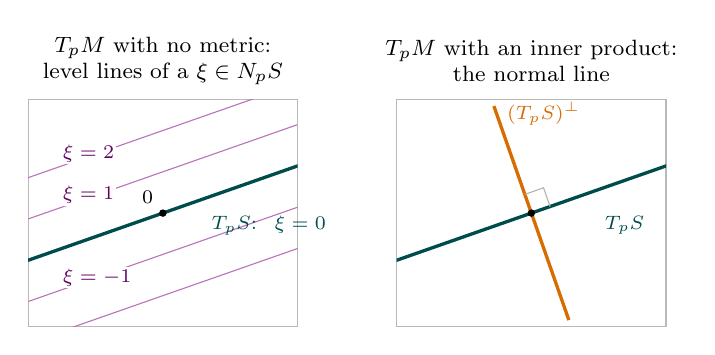
\begin{tikzpicture}[scale=0.9]
\draw[gray!55] (-1.90,-1.6) rectangle (1.90,1.6);
\node[font=\footnotesize, align=center] at (0.00,2.15){$T_pM$ with no metric:\\ level lines of a $\xi \in N_pS$};
\begin{scope}\clip (-1.9,-1.6) rectangle (1.9,1.6); \draw[violet!55] (-1.713,-1.765) -- (2.440,-0.311); \end{scope}
\begin{scope}\clip (-1.9,-1.6) rectangle (1.9,1.6); \draw[violet!55] (-1.895,-1.246) -- (2.258,0.208); \end{scope}
\begin{scope}\clip (-1.9,-1.6) rectangle (1.9,1.6); \draw[violet!55] (-2.258,-0.208) -- (1.895,1.246); \end{scope}
\begin{scope}\clip (-1.9,-1.6) rectangle (1.9,1.6); \draw[violet!55] (-2.440,0.311) -- (1.713,1.765); \end{scope}


\begin{scope}\clip (-1.9,-1.6) rectangle (1.9,1.6); \draw[teal!60!black, very thick] (-2.076,-0.727) -- (2.076,0.727); \end{scope}
\node[teal!60!black, font=\scriptsize, anchor=north west] at (0.55,0.1) {$T_pS$: \ $\xi = 0$};
\fill (0,0) circle (1.5pt) node[above left, font=\scriptsize] {$0$};
\draw[gray!55] (3.30,-1.6) rectangle (7.10,1.6);
\node[font=\footnotesize, align=center] at (5.20,2.15){$T_pM$ with an inner product:\\ the normal line};
\begin{scope}\clip (3.30,-1.6) rectangle (7.10,1.6); \draw[teal!60!black, very thick] (3.124,-0.727) -- (7.276,0.727); \end{scope}
\draw[orange!85!black, very thick] (5.729,-1.510) -- (4.671,1.510);
\draw[gray!60] (5.464,0.092) -- (5.372,0.357) -- (5.108,0.264);
\node[teal!60!black, font=\scriptsize, anchor=north west] at (6.10,0.1) {$T_pS$};
\node[orange!85!black, font=\scriptsize, anchor=west] at (4.721,1.410) {$(T_pS)^\perp$};
\fill (5.20,0) circle (1.5pt);
\node[violet!75!black, font=\scriptsize, fill=white, inner sep=0.8pt, anchor=south west] at (-1.450,0.095) {$\xi = 1$};
\node[violet!75!black, font=\scriptsize, fill=white, inner sep=0.8pt, anchor=south west] at (-1.450,0.678) {$\xi = 2$};
\node[violet!75!black, font=\scriptsize, fill=white, inner sep=0.8pt, anchor=south west] at (-1.450,-1.070) {$\xi = -1$};
\end{tikzpicture}
\end{center}

How to draw a conormal covector. Without a metric, a covector $\xi$ on $T_pM$ is drawn by its level lines $\{\xi = \text{const}\}$. For $\xi \in N_pS$ the level line $\xi = 0$ contains $T_pS$, so all of its level lines run \emph{parallel} to $T_pS$ (left). Only once an inner product is chosen does $\xi$ become a vector, perpendicular to its level lines, and $N_pS$ becomes the normal line $(T_pS)^\perp$ (right). The board, and page~33 of the handwritten notes, draw $N_pS$ as a line perpendicular to $T_pS$: that is the right-hand, metric picture.

\subsection{The Regular Value Theorem for Manifolds}\label{sub:rvt-manifolds}

\textit{Lecture 12. ``And now we go back to submersions'' --- to ``[the] wonderful version of the regular value theorem.''}

\begin{thmbox}[The Regular Value Theorem for Manifolds]\thmlabel{thm:rvt-manifolds}
Let $F : M \to N$ be smooth, with $\dim M = m$ and $\dim N = n$, and let $q \in N$ be a regular value of $F$ (Definition~\ref{def:regular-critical}). Then $S = F^{-1}(q)$ is a submanifold of $M$ of codimension $n$ (possibly empty), so $\dim S = m - n$, and for every $p \in S$
\[
\iota_{*p}(T_pS) = \ker F_{*p} .
\]
\leeref{Corollary 5.14 and Proposition 5.38}
\end{thmbox}

\begin{proof}
\emph{$S$ is a submanifold (Lecture~12).} We check the definition at each $p \in S$: we need an adapted chart at $p$. By assumption $F$ is a submersion at $p$, so the normal form (Theorem~\ref{thm:submersion-normal-form}) gives charts $(U, \hat\varphi = (x^1, \ldots, x^m))$ at $p$ and $(V, \psi = (y^1, \ldots, y^n))$ at $q = F(p)$, with $F(U) \subseteq V$ and $\tilde F(r^1, \ldots, r^m) = (r^1, \ldots, r^n)$. What are the equations of $S \cap U$ in these coordinates? For $q' \in U$,
\begin{align*}
q' \in S &\iff F(q') = q \iff \psi\big(F(q')\big) = \psi(q) \\
&\iff \tilde F\big(\hat\varphi(q')\big) = \psi(q) \iff \big(x^1(q'), \ldots, x^n(q')\big) = \big(y^1(q), \ldots, y^n(q)\big).
\end{align*}
``These are not of the type $x_b = 0$, but of the type $x_a$ equals a constant'': the first $n$ coordinates equal a constant vector. By the observations after the definition (Proposition~\ref{prop:adapted-flex}) --- any constant, and any $n$ of the coordinates --- $S$ has an adapted chart at $p$, of codimension $n$. \textit{(Completion.)} The second equivalence uses that $\psi$ is injective on $V$, which contains $F(q')$; the last is the normal form.

\emph{The tangent space.} \textit{(Completion. In lecture: ``I won't bother checking the kernel thing, because everything really reduces to the Euclidean [case].'')} The composite $F \circ \iota : S \to N$ is constant, with value $q$, and the pushforward along a constant map is zero (as in the proof of Theorem~\ref{thm:tangent-product}); so $F_{*p} \circ \iota_{*p} = 0$ and $\iota_{*p}(T_pS) \subseteq \ker F_{*p}$. The left side has dimension $m - n$, since $\iota_{*p}$ is injective (Proposition~\ref{prop:submanifold-tangent}); the right side has dimension $m - n$ by rank--nullity, since $F_{*p}$ is onto (Proposition~\ref{fact:linalg}). A subspace of the same finite dimension is everything, so the two are equal. This is the argument of Lecture~8 for $T^{\geo}_pM = \ker F'(p)$ (Theorem~\ref{thm:tangent-kernel}), one level up.
\end{proof}

\begin{center}
\begin{tikzcd}[column sep=6em, row sep=3em]
S \cap U \subseteq U \arrow[r, "F"] \arrow[d, "\hat\varphi"'] & V \ni q \arrow[d, "\psi"] \\
\big\{ r : (r^1, \ldots, r^n) = \psi(q) \big\} \subseteq \hat\varphi(U) \arrow[r, "\tilde F"'] & \psi(V) \ni \psi(q)
\end{tikzcd}
\end{center}

The proof in one square, as on the board. In the normal-form charts $\tilde F$ is the projection onto the first $n$ coordinates, so the level set $S \cap U = F^{-1}(q) \cap U$ is carried by $\hat\varphi$ onto a fibre of a projection: the slice where the first $n$ coordinates equal $\psi(q)$.

\textbf{Transcription note.} Page~33 of the handwritten notes states the theorem for ``$q \in M$ a regular value''; the regular value lies in the target, $q \in N$.

\begin{corbox}[Fibres of Submersions Are Submanifolds]\thmlabel{cor:submersion-fibres}
If $F : M \to N$ is a submersion, then every fibre $F^{-1}(q)$, $q \in N$, is a submanifold of $M$ of codimension $n$ --- ``they could be empty, some of them.''
\end{corbox}

\begin{proof}
Every $q \in N$ is a regular value: every point of $F^{-1}(q)$ is a regular point, and if $F^{-1}(q)$ is empty the condition holds vacuously. Apply Theorem~\ref{thm:rvt-manifolds}.
\end{proof}

\begin{rembox}[The Regular Value Theorems --- Old and New]\label{rem:regular-value-theorems-old-new}
The notes now contain the regular value theorem in five forms. They are one idea met at increasing generality, not competing statements.
\begin{center}
\renewcommand{\arraystretch}{1.2}
\begin{tabular}{>{\raggedright\arraybackslash}p{2.5cm} >{\raggedright\arraybackslash}p{2.9cm} >{\raggedright\arraybackslash}p{3.0cm} >{\raggedright\arraybackslash}p{3.0cm}}
\toprule
\textbf{Where} & \textbf{Setting} & \textbf{Conclusion} & \textbf{Role now} \\ \midrule
Thm.~\ref{thm:regular-value}, Cor.~\ref{cor:rvt-open} & $F : W \to \mathbb{R}^k$, $W \subseteq \mathbb{R}^{n+k}$ open & topological manifold & the first version (Lecture~3); Chapter~2 needs it \\
Prop.~\ref{prop:level-set-smooth} & the same & smooth manifold, by graph charts & the Euclidean case (Lecture~6) \\
Prop.~\ref{prop:regular-one-chart} & $F : M \to N$, level set inside one chart & regular for $F$ iff for $\tilde F$ & a computational tool \\
Cor.~\ref{cor:manifold-level-sets} & $F : M \to N$ & topological manifold & subsumed; a more elementary proof \\
Thm.~\ref{thm:rvt-manifolds} & $F : M \to N$ & submanifold, with $\iota_{*p}(T_pS) = \ker F_{*p}$ & the general theorem (Lecture~12) \\
\bottomrule
\end{tabular}
\end{center}
The general theorem contains the others: taking $M$ an open subset of Euclidean space recovers the first two. Its proof goes through the normal form, which rests on the inverse function theorem and not on \ref{sec:rvt}, so nothing is circular. The next proposition shows that the old and new versions give the same smooth structure and the same tangent spaces.
\end{rembox}

\begin{propbox}[The Old and New Versions Agree]\thmlabel{prop:rvt-agree}
Let $W \subseteq \mathbb{R}^{n+k}$ be open, $F : W \to \mathbb{R}^k$ smooth, $c$ a regular value, and $S = F^{-1}(c)$.
\begin{enumerate}
    \item The smooth structure on $S$ given by the graph charts (Proposition~\ref{prop:level-set-smooth}) is the induced structure of $S$ as a submanifold of $W$ (Theorem~\ref{thm:rvt-manifolds}).
    \item In the setting of Theorem~\ref{thm:ambient-abstract}, under the identification $T_pW = \mathbb{R}^{n+k}$ of Corollary~\ref{cor:tangent-vs}, the subspace $\iota_{*p}(T_pS)$ is $T^{\geo}_pS = \ker F'(p)$.
\end{enumerate}
\end{propbox}

\begin{proof}
\textit{(Not from lecture; filled in.)} First, $c$ is a regular value in both senses, since the matrix of $F_{*p}$ in the standard coordinates is $F'(p)$ (Theorem~\ref{lem:differential-matrix}).

(1) Let $p \in S$. As in the construction of the graph charts, after reordering the coordinates write the points of $\mathbb{R}^{n+k}$ as $(x, y) \in \mathbb{R}^n \times \mathbb{R}^k$ with $\partial F/\partial y\,(p)$ invertible, so that the graph chart near $p$ is $(x, y) \mapsto x$ on $S$. Let $\Phi(x, y) = (x, F(x, y) - c)$. Its Jacobian at $p$ is $\begin{pmatrix} I_n & 0 \\ \partial F/\partial x & \partial F/\partial y \end{pmatrix}$, which is invertible, so by the inverse function theorem $\Phi$ restricts to a diffeomorphism of an open $U \ni p$ onto an open set, and by Lemma~\ref{lem:diffeo-chart} it is a smooth chart of $W$. Its last $k$ components are $F - c$, which vanish exactly on $S \cap U$, so $\Phi$ is adapted, and its induced chart is $\Phi_S = x|_{S \cap U}$: the graph chart. So near each of its points, every graph chart is an induced chart. Induced charts are pairwise compatible, and smoothness of a transition map is local, so every graph chart is compatible with every induced chart, and the two atlases determine the same maximal atlas (Theorem~\ref{thm:maximal-atlas}).

(2) Let $v \in T^{\geo}_pS$, and let $\gamma$ be the lifted line of Definition~\ref{def:Dv}, a curve in $S$ with $\gamma(0) = p$ and $\gamma'(0) = v$, so that $D_v = D_\gamma$. By Corollary~\ref{cor:velocity-composite}, $\iota_{*p}D_v = D_{\iota \circ \gamma}$, the derivation $g \mapsto (g \circ \gamma)'(0) = \nabla g(p) \cdot v$ at $p$ --- the directional derivative in the direction $v$, which is $v$ under Corollary~\ref{cor:tangent-vs}. Since $v \mapsto D_v$ is onto $T_pS$ (Theorem~\ref{thm:ambient-abstract}), $\iota_{*p}(T_pS) = T^{\geo}_pS$, and $T^{\geo}_pS = \ker F'(p)$ by Theorem~\ref{thm:tangent-kernel}. This matches $\ker F_{*p}$ in Theorem~\ref{thm:rvt-manifolds}, $F_{*p}$ being $F'(p)$.
\end{proof}

\section{Fibrations}\label{sec:fibrations}

\roadmark{Stage: bundles}{Submersions that are locally products.}

\textit{References: Lee Ch.~10. Lectures 11--13.} The submersions that look locally like the projection $U \times F \to U$. Their fibres are submanifolds (\ref{sec:submanifolds}), all copies of one fibre; the tangent bundle of the next section is the first major example.

\subsection{Fibrations}\label{sub:fibrations}

\textit{Lecture 11. ``An important class within the submersions.'' Uribe introduced fibrations now because the tangent bundle, the cotangent bundle and vector bundles, coming soon, are all fibrations. The idea: surjective maps $\pi : M \to B$ that are locally like the projection $U \times F \to U$, with $U$ open in the \textbf{base} $B$ and $F$ a third, fixed manifold. There is a notation clash he apologized for --- $F$ now names the fibre, not the map, which is called $\pi$.}

\begin{defbox}[Fibration]\deflabel{def:fibration}
Let $M$, $B$ and $F$ be smooth manifolds and $\pi : M \to B$ smooth. Then $\pi$ is a \textbf{fibration with fibre $F$} if there are an open cover $\{U_\alpha\}_{\alpha \in A}$ of $B$ and, for each $\alpha$, a diffeomorphism
\[
\phi_\alpha : \pi^{-1}(U_\alpha) \longrightarrow U_\alpha \times F \qquad \text{with} \qquad \mathrm{pr}_1 \circ \phi_\alpha = \pi|_{\pi^{-1}(U_\alpha)},
\]
where $\pi^{-1}(U_\alpha)$ is an open submanifold of $M$, $U_\alpha \times F$ a product manifold (Definition~\ref{def:product-manifold}), and $\mathrm{pr}_1 : U_\alpha \times F \to U_\alpha$ the projection. The $\phi_\alpha$ are called \textbf{local trivializations}. $M$ is the \textbf{total space} and $B$ the \textbf{base}.
\leeref{Ch.~10, smooth fiber bundles}
\end{defbox}

\begin{center}
\begin{tikzcd}[row sep=3em, column sep=4.5em]
\pi^{-1}(U_\alpha) \arrow[rr, "\phi_\alpha", "\cong"'] \arrow[dr, "\pi|"'] & & U_\alpha \times F \arrow[dl, "\mathrm{pr}_1"] \\
& U_\alpha \subseteq B &
\end{tikzcd}
\end{center}

The diagram \emph{commutes}. A student asked what that means; Uribe: ``whenever you have a diagram \ldots\ all the compositions that you can construct from one place to another give you the same answer.'' Here there are two routes from $\pi^{-1}(U_\alpha)$ to $U_\alpha$, and they agree: $\mathrm{pr}_1 \circ \phi_\alpha = \pi|$. Concretely, $\phi_\alpha(p) = (\pi(p), \ast)$ --- its first component \emph{is} $\pi(p)$, and only the second, a point of $F$, is new information.

\begin{center}
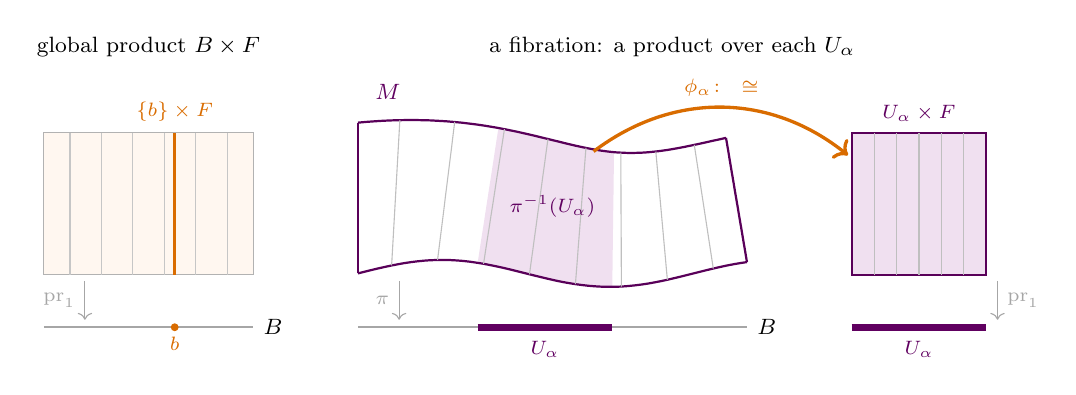
\begin{tikzpicture}[scale=0.95]
\fill[orange!6] (0,0.7) rectangle (2.8,2.6); \draw[gray!60] (0,0.7) rectangle (2.8,2.6);
\draw[gray!45] (0.35,0.7) -- (0.35,2.6);
\draw[gray!45] (0.77,0.7) -- (0.77,2.6);
\draw[gray!45] (1.19,0.7) -- (1.19,2.6);
\draw[gray!45] (1.61,0.7) -- (1.61,2.6);
\draw[gray!45] (2.03,0.7) -- (2.03,2.6);
\draw[gray!45] (2.45,0.7) -- (2.45,2.6);
\draw[orange!85!black, very thick] (1.75,0.7) -- (1.75,2.6); \node[orange!85!black, font=\scriptsize, anchor=south] at (1.75,2.62) {$\{b\} \times F$};
\draw[thick, gray!70] (0,0) -- (2.8,0) node[right, font=\footnotesize, text=black] {$B$}; \fill[orange!85!black] (1.75,0) circle (1.5pt) node[below, font=\scriptsize] {$b$};
\draw[->, gray!70] (0.55,0.62) -- node[left, font=\scriptsize] {$\mathrm{pr}_1$} (0.55,0.1);
\node[font=\footnotesize] at (1.4,3.75) {global product $B \times F$};
\fill[violet!12] (5.800,0.861) -- (5.825,1.025) -- (5.850,1.189) -- (5.876,1.353) -- (5.901,1.517) -- (5.926,1.680) -- (5.951,1.844) -- (5.977,2.008) -- (6.002,2.172) -- (6.027,2.336) -- (6.052,2.500) -- (6.078,2.663) -- (6.078,2.663) -- (6.174,2.645) -- (6.269,2.626) -- (6.362,2.606) -- (6.453,2.586) -- (6.542,2.565) -- (6.628,2.544) -- (6.713,2.523) -- (6.796,2.503) -- (6.878,2.483) -- (6.958,2.463) -- (7.036,2.444) -- (7.113,2.427) -- (7.188,2.410) -- (7.262,2.395) -- (7.336,2.381) -- (7.408,2.368) -- (7.480,2.357) -- (7.552,2.348) -- (7.623,2.341) -- (7.623,2.341) -- (7.621,2.177) -- (7.619,2.013) -- (7.617,1.850) -- (7.615,1.686) -- (7.612,1.522) -- (7.610,1.359) -- (7.608,1.195) -- (7.606,1.031) -- (7.604,0.868) -- (7.602,0.704) -- (7.600,0.540) -- (7.600,0.540) -- (7.505,0.541) -- (7.411,0.544) -- (7.316,0.551) -- (7.221,0.561) -- (7.126,0.573) -- (7.032,0.588) -- (6.937,0.605) -- (6.842,0.625) -- (6.747,0.646) -- (6.653,0.668) -- (6.558,0.691) -- (6.463,0.715) -- (6.368,0.739) -- (6.274,0.763) -- (6.179,0.785) -- (6.084,0.807) -- (5.989,0.827) -- (5.895,0.845) -- (5.800,0.861) -- cycle;
\draw[violet!70!black, thick] (4.200,0.720) -- (4.288,0.742) -- (4.376,0.764) -- (4.464,0.785) -- (4.553,0.805) -- (4.641,0.824) -- (4.729,0.841) -- (4.817,0.857) -- (4.905,0.870) -- (4.993,0.881) -- (5.081,0.890) -- (5.169,0.896) -- (5.258,0.899) -- (5.346,0.900) -- (5.434,0.898) -- (5.522,0.893) -- (5.610,0.886) -- (5.698,0.876) -- (5.786,0.863) -- (5.875,0.849) -- (5.963,0.832) -- (6.051,0.814) -- (6.139,0.795) -- (6.227,0.774) -- (6.315,0.752) -- (6.403,0.730) -- (6.492,0.708) -- (6.580,0.686) -- (6.668,0.665) -- (6.756,0.644) -- (6.844,0.624) -- (6.932,0.606) -- (7.020,0.590) -- (7.108,0.576) -- (7.197,0.564) -- (7.285,0.554) -- (7.373,0.547) -- (7.461,0.542) -- (7.549,0.540) -- (7.637,0.541) -- (7.725,0.544) -- (7.814,0.551) -- (7.902,0.560) -- (7.990,0.571) -- (8.078,0.584) -- (8.166,0.600) -- (8.254,0.617) -- (8.342,0.636) -- (8.431,0.657) -- (8.519,0.678) -- (8.607,0.700) -- (8.695,0.722) -- (8.783,0.744) -- (8.871,0.766) -- (8.959,0.787) -- (9.047,0.807) -- (9.136,0.826) -- (9.224,0.843) -- (9.312,0.858) -- (9.400,0.871); \draw[violet!70!black, thick] (4.200,2.735) -- (4.310,2.745) -- (4.421,2.753) -- (4.530,2.760) -- (4.640,2.765) -- (4.749,2.768) -- (4.857,2.770) -- (4.965,2.770) -- (5.071,2.768) -- (5.177,2.765) -- (5.281,2.759) -- (5.384,2.753) -- (5.486,2.744) -- (5.586,2.735) -- (5.685,2.723) -- (5.782,2.711) -- (5.878,2.697) -- (5.971,2.682) -- (6.064,2.666) -- (6.154,2.649) -- (6.243,2.631) -- (6.330,2.613) -- (6.415,2.594) -- (6.498,2.575) -- (6.580,2.556) -- (6.660,2.536) -- (6.738,2.517) -- (6.815,2.498) -- (6.891,2.480) -- (6.965,2.461) -- (7.037,2.444) -- (7.109,2.427) -- (7.179,2.412) -- (7.249,2.397) -- (7.317,2.384) -- (7.385,2.372) -- (7.452,2.361) -- (7.518,2.352) -- (7.585,2.344) -- (7.651,2.338) -- (7.717,2.334) -- (7.783,2.331) -- (7.849,2.330) -- (7.915,2.331) -- (7.982,2.333) -- (8.050,2.337) -- (8.118,2.343) -- (8.187,2.350) -- (8.258,2.359) -- (8.329,2.369) -- (8.401,2.381) -- (8.475,2.394) -- (8.550,2.408) -- (8.627,2.424) -- (8.705,2.440) -- (8.784,2.457) -- (8.866,2.475) -- (8.949,2.494) -- (9.034,2.512) -- (9.120,2.532);
\draw[violet!70!black, thick] (4.200,0.720) -- (4.200,0.903) -- (4.200,1.086) -- (4.200,1.270) -- (4.200,1.453) -- (4.200,1.636) -- (4.200,1.819) -- (4.200,2.002) -- (4.200,2.186) -- (4.200,2.369) -- (4.200,2.552) -- (4.200,2.735); \draw[violet!70!black, thick] (9.400,0.871) -- (9.375,1.022) -- (9.349,1.173) -- (9.324,1.324) -- (9.298,1.475) -- (9.273,1.626) -- (9.247,1.777) -- (9.222,1.928) -- (9.196,2.079) -- (9.171,2.230) -- (9.146,2.381) -- (9.120,2.532);
\draw[gray!50] (4.650,0.826) -- (4.660,1.003) -- (4.670,1.179) -- (4.680,1.356) -- (4.690,1.532) -- (4.700,1.709) -- (4.710,1.886) -- (4.720,2.062) -- (4.730,2.239) -- (4.740,2.415) -- (4.750,2.592) -- (4.760,2.768);
\draw[gray!50] (5.264,0.899) -- (5.285,1.067) -- (5.306,1.235) -- (5.327,1.402) -- (5.348,1.570) -- (5.368,1.738) -- (5.389,1.905) -- (5.410,2.073) -- (5.431,2.241) -- (5.452,2.408) -- (5.472,2.576) -- (5.493,2.744);
\draw[gray!50] (5.879,0.848) -- (5.904,1.012) -- (5.929,1.175) -- (5.955,1.339) -- (5.980,1.503) -- (6.006,1.666) -- (6.031,1.830) -- (6.056,1.994) -- (6.082,2.157) -- (6.107,2.321) -- (6.133,2.485) -- (6.158,2.648);
\draw[gray!50] (6.493,0.708) -- (6.515,0.872) -- (6.538,1.037) -- (6.560,1.201) -- (6.583,1.366) -- (6.605,1.530) -- (6.627,1.695) -- (6.650,1.859) -- (6.672,2.023) -- (6.695,2.188) -- (6.717,2.352) -- (6.740,2.517);
\draw[gray!50] (7.107,0.576) -- (7.120,0.741) -- (7.133,0.907) -- (7.145,1.073) -- (7.158,1.238) -- (7.171,1.404) -- (7.184,1.570) -- (7.196,1.735) -- (7.209,1.901) -- (7.222,2.066) -- (7.235,2.232) -- (7.248,2.398);
\draw[gray!50] (7.721,0.544) -- (7.721,0.707) -- (7.720,0.870) -- (7.719,1.032) -- (7.719,1.195) -- (7.718,1.358) -- (7.717,1.520) -- (7.716,1.683) -- (7.716,1.846) -- (7.715,2.009) -- (7.714,2.171) -- (7.714,2.334);
\draw[gray!50] (8.336,0.635) -- (8.322,0.791) -- (8.308,0.947) -- (8.294,1.102) -- (8.280,1.258) -- (8.266,1.414) -- (8.252,1.570) -- (8.238,1.726) -- (8.224,1.882) -- (8.210,2.038) -- (8.196,2.194) -- (8.182,2.349);
\draw[gray!50] (8.950,0.785) -- (8.927,0.935) -- (8.904,1.085) -- (8.881,1.236) -- (8.858,1.386) -- (8.835,1.536) -- (8.812,1.687) -- (8.789,1.837) -- (8.766,1.987) -- (8.742,2.138) -- (8.719,2.288) -- (8.696,2.438);
\node[violet!75!black, font=\footnotesize] at (4.60,3.15) {$M$};
\node[violet!75!black, font=\scriptsize] at (6.80,1.62) {$\pi^{-1}(U_\alpha)$};
\draw[thick, gray!70] (4.20,0) -- (9.40,0) node[right, font=\footnotesize, text=black] {$B$};
\draw[violet!75!black, line width=2.4pt] (5.80,0) -- (7.60,0); \node[violet!75!black, font=\scriptsize] at (6.70,-0.3) {$U_\alpha$};
\draw[->, gray!70] (4.75,0.62) -- node[left, font=\scriptsize] {$\pi$} (4.75,0.1);
\fill[violet!12] (10.80,0.7) rectangle (12.60,2.6); \draw[violet!70!black, thick] (10.80,0.7) rectangle (12.60,2.6);
\draw[gray!50] (11.10,0.7) -- (11.10,2.6);
\draw[gray!50] (11.40,0.7) -- (11.40,2.6);
\draw[gray!50] (11.70,0.7) -- (11.70,2.6);
\draw[gray!50] (12.00,0.7) -- (12.00,2.6);
\draw[gray!50] (12.30,0.7) -- (12.30,2.6);
\node[violet!75!black, font=\scriptsize, anchor=south] at (11.70,2.62) {$U_\alpha \times F$};
\draw[violet!75!black, line width=2.4pt] (10.80,0) -- (12.60,0); \node[violet!75!black, font=\scriptsize] at (11.70,-0.3) {$U_\alpha$};
\draw[->, gray!70] (12.75,0.62) -- node[right, font=\scriptsize] {$\mathrm{pr}_1$} (12.75,0.1);
\draw[->, very thick, orange!85!black] (7.35,2.35) to[bend left=38] node[above, font=\scriptsize] {$\phi_\alpha \colon\ \cong$} (10.75,2.3);
\node[font=\footnotesize] at (8.40,3.75) {a fibration: a product over each $U_\alpha$};
\end{tikzpicture}
\end{center}

Uribe's cartoon, and why it matters: ``these cartoons are incredibly important.'' On the left, the global product $B \times F$, with each fibre $\{b\} \times F$ standing over its point. On the right, a total space that need not be a product: its fibres may twist as they travel over $B$. But over each $U_\alpha$ the part $\pi^{-1}(U_\alpha)$ is identified by $\phi_\alpha$ with the straight product $U_\alpha \times F$, and the identification respects the base points, which is the commuting diagram.

\begin{propbox}[Fibres and Fibrations]\thmlabel{prop:fibration-properties}
Let $\pi : M \to B$ be a fibration with fibre $F$.
\begin{enumerate}
    \item For every $b \in B$, the fibre $\pi^{-1}(b)$ is homeomorphic to $F$: every fibre is a copy of the model fibre.
    \item $\pi$ is a submersion, and it is surjective if $F \ne \emptyset$.
    \item $\pi$ is an open map.
\end{enumerate}
\end{propbox}

\begin{proof}
\textit{(Stated in lecture; (2) as ``chain rule and stuff''.)} (1) Choose $\alpha$ with $b \in U_\alpha$. Because the diagram commutes and $\phi_\alpha$ is a bijection, $\phi_\alpha$ maps $\pi^{-1}(b)$ onto $\mathrm{pr}_1^{-1}(b) = \{b\} \times F$; it restricts to a homeomorphism with the subspace topologies. And $\{b\} \times F \to F$, $(b, f) \mapsto f$, is a homeomorphism, with inverse $f \mapsto (b, f)$. (2) On the open set $\pi^{-1}(U_\alpha)$, $\pi = \mathrm{pr}_1 \circ \phi_\alpha$; by the Chain Rule $\pi_{*p} = (\mathrm{pr}_1)_{*} \circ (\phi_\alpha)_{*p}$, a composite of an isomorphism and a surjection (Example~\ref{ex:product-projection-submersion}), hence onto. Every $b$ lies in some $U_\alpha$, and its fibre is a copy of $F$, nonempty if $F$ is. (3) Corollary~\ref{cor:submersion-open-map}.
\end{proof}

The Hopf fibration $S^{2n+1} \to \mathbb{CP}^n$, the first example of a fibration, and its local but not global sections are collected in Section~\ref{sec:ex-hopf}.

\begin{rembox}[What Comes Next]\label{rem:what-comes-next}
Tangent bundles, cotangent bundles and vector bundles are fibrations ``with additional structure, where the fibres are vector spaces.'' The basic notion of fibration is more general: its fibre $F$ is any manifold.
\end{rembox}

\textbf{Transcription note.} Stating the idea of a fibration, Uribe first said ``$U$ open in $M$''; a student corrected it to open in $B$, as in the definition.

\subsection{Fibres and Examples}\label{sub:fibrations-revisited}

\textit{Lecture 12. Uribe changed the notation once more ``to conform to more general usage'': the fibration is $\pi : E \to B$, with total space $E$, base $B$, and fibre $F$ --- the definition as before (Definition~\ref{def:fibration}), with $E$ in place of $M$.}

\begin{propbox}[Fibres Are Copies of the Model Fibre]\thmlabel{prop:fibres-diffeo}
Let $\pi : E \to B$ be a fibration with fibre $F$ and $b \in B$. Then $\pi^{-1}(b)$ is a submanifold of $E$, and for every $\alpha$ with $b \in U_\alpha$ the local trivialization $\phi_\alpha$ restricts to a diffeomorphism
\[
\pi^{-1}(b) \longrightarrow \{b\} \times F \cong F .
\]
\end{propbox}

\begin{proof}
\textit{(Claimed in Lecture~12 --- ``I claim that they are diffeomorphic to this fibre, to the third manifold that is sitting outside, looking over [the] landscape''; filled in.)} $\pi$ is a submersion (Proposition~\ref{prop:fibration-properties}), so $\pi^{-1}(b)$ is a submanifold (Corollary~\ref{cor:submersion-fibres}); likewise $\{b\} \times F = \mathrm{pr}_1^{-1}(b)$ is a submanifold of $U_\alpha \times F$ (Example~\ref{ex:product-projection-submersion}). Because the diagram commutes, $\phi_\alpha$ maps $\pi^{-1}(b)$ bijectively onto $\{b\} \times F$. The restriction and its inverse are smooth as maps into $U_\alpha \times F$ and into $E$ (restrictions of $\phi_\alpha$, $\phi_\alpha^{-1}$ to submanifolds, Lemma~\ref{lem:maps-into-submanifold}(1)), hence smooth into the submanifolds $\{b\} \times F$ and $\pi^{-1}(b)$ (Lemma~\ref{lem:maps-into-submanifold}(2)). Finally $\{b\} \times F \to F$, $(b, f) \mapsto f$, is a diffeomorphism by the same lemma, with inverse $f \mapsto (b, f)$.
\end{proof}

\begin{center}
\begin{tikzcd}[column sep=4.4em, row sep=2.8em]
\pi^{-1}(b) \arrow[r, hook] \arrow[d, "\phi_\alpha|"', "\cong"] & \pi^{-1}(U_\alpha) \arrow[d, "\phi_\alpha", "\cong"'] \\
\{b\} \times F \arrow[r, hook] \arrow[d, "\mathrm{pr}_2"', "\cong"] & U_\alpha \times F \\
F &
\end{tikzcd}
\end{center}

The fibre over $b$ and the model fibre. The trivialization $\phi_\alpha$ carries the submanifold $\pi^{-1}(b)$ onto the submanifold $\{b\} \times F$ --- this is where the commuting triangle of Definition~\ref{def:fibration} is used --- and $\mathrm{pr}_2$ identifies that with $F$.

This upgrades Proposition~\ref{prop:fibration-properties}(1) from homeomorphic to diffeomorphic. Not every submersion has this property: its fibres are submanifolds, but they can change type from one point to another.

\begin{exbox}[A Submersion That Is Not a Fibration]\exlabel{ex:punctured-plane}
Let $E = \mathbb{R}^2 \setminus \{(0, 1)\}$ and $\pi : E \to \mathbb{R}$, $\pi(x, y) = x$. Then $\pi$ is a surjective submersion, but not a fibration.
\end{exbox}

\begin{proof}
\textit{(Lecture~12.)} $\pi$ is the restriction of the projection $\mathbb{R}^2 \to \mathbb{R}$ to an open subset, so it is a submersion (Example~\ref{ex:projection-submersion}), and it is onto. Its fibres are the vertical lines $\{x\} \times \mathbb{R}$ for $x \ne 0$, ``except for one'': over $0$ the fibre is $\{0\} \times (\mathbb{R} \setminus \{1\})$, two half-lines --- ``it wants to be a vertical line, but there's a point missing.'' If $\pi$ were a fibration with fibre $F$, all fibres would be diffeomorphic to $F$ (Proposition~\ref{prop:fibres-diffeo}), hence to each other; but $\{1\} \times \mathbb{R}$ is connected and $\{0\} \times (\mathbb{R} \setminus \{1\})$ is not, and connectedness is preserved by homeomorphisms.
\end{proof}

\begin{center}
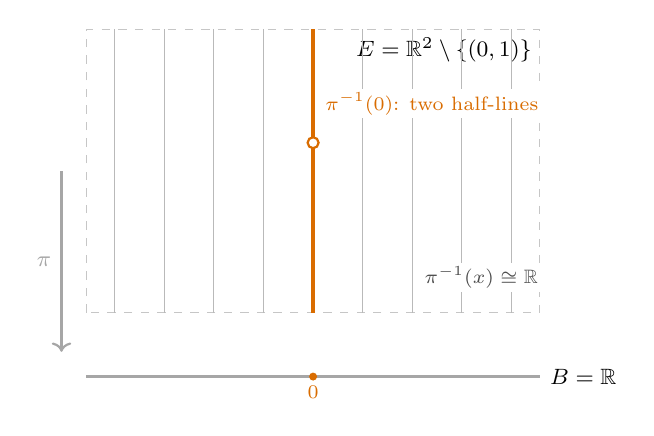
\begin{tikzpicture}[scale=0.9]
\draw[gray!45, dashed] (-3.2,-1.4) rectangle (3.2,2.6); \node[font=\footnotesize, anchor=north east, fill=white, inner sep=1.5pt] at (3.15,2.55) {$E = \mathbb{R}^2 \setminus \{(0,1)\}$};
\draw[gray!55] (-2.80,-1.4) -- (-2.80,2.6);
\draw[gray!55] (-2.10,-1.4) -- (-2.10,2.6);
\draw[gray!55] (-1.40,-1.4) -- (-1.40,2.6);
\draw[gray!55] (-0.70,-1.4) -- (-0.70,2.6);
\draw[gray!55] (0.70,-1.4) -- (0.70,2.6);
\draw[gray!55] (1.40,-1.4) -- (1.40,2.6);
\draw[gray!55] (2.10,-1.4) -- (2.10,2.6);
\draw[gray!55] (2.80,-1.4) -- (2.80,2.6);
\draw[orange!85!black, very thick] (0,-1.4) -- (0,0.93); \draw[orange!85!black, very thick] (0,1.07) -- (0,2.6);
\draw[orange!85!black, fill=white, thick] (0,1) circle (2.2pt);
\node[orange!85!black, font=\scriptsize, anchor=west, align=left, fill=white, inner sep=1.2pt] at (0.12,1.55) {$\pi^{-1}(0)$: two half-lines};
\node[gray!60!black, font=\scriptsize, anchor=west, fill=white, inner sep=1.2pt] at (1.52,-0.9) {$\pi^{-1}(x) \cong \mathbb{R}$};
\draw[->, thick, gray!70] (-3.55,0.6) -- node[left, font=\footnotesize] {$\pi$} (-3.55,-1.95);
\draw[thick, gray!70] (-3.2,-2.3) -- (3.2,-2.3) node[right, font=\footnotesize, text=black] {$B = \mathbb{R}$};
\fill[orange!85!black] (0,-2.3) circle (1.6pt) node[below, font=\scriptsize] {$0$};
\end{tikzpicture}
\end{center}

The punctured plane over the $x$-axis. Every fibre is a whole vertical line except the one over $0$, which is broken at the missing point into two half-lines. The fibres are all submanifolds (Corollary~\ref{cor:submersion-fibres}), but not all of the same type.

A student asked the converse: if all the fibres of a surjective submersion are diffeomorphic to one manifold, must it be a fibration? Uribe: ``I don't think that's true, but I don't have a quick example.'' He answered it at the start of Lecture~13: yes when $\pi$ is proper, no in general (Theorem~\ref{thm:ehresmann} and Example~\ref{ex:ehresmann-counter} below).

\begin{exbox}[The Möbius Band]\exlabel{ex:mobius}
The Möbius band fibres over its core circle, with an interval as fibre: ``no matter where you cut it, it just looks like a [strip]. But globally, it's not a product.'' Concretely, let $E = \big(\mathbb{R} \times (-1, 1)\big)/{\sim}$ with $(s, t) \sim (s + n, (-1)^n t)$ for $n \in \mathbb{Z}$, and $\pi[s, t] = [s] \in \mathbb{R}/\mathbb{Z} \cong S^1$.
\leeref{Example 10.3}
\end{exbox}

\textit{Status.} In lecture this was a picture, not a proof: the claims that $\pi$ is a fibration with fibre $(-1, 1)$, and that $E$ is not globally the product $S^1 \times (-1, 1)$, are stated, not proved, here. Over any arc of the circle shorter than the whole, the twist can be undone, which is the local product structure; the obstruction is global, and it is visible in the picture: the band has a single boundary curve, while the product $S^1 \times (-1, 1)$ closed up would have two. Lee's Möbius bundle takes the fibre $\mathbb{R}$ in place of $(-1, 1)$.

\begin{center}
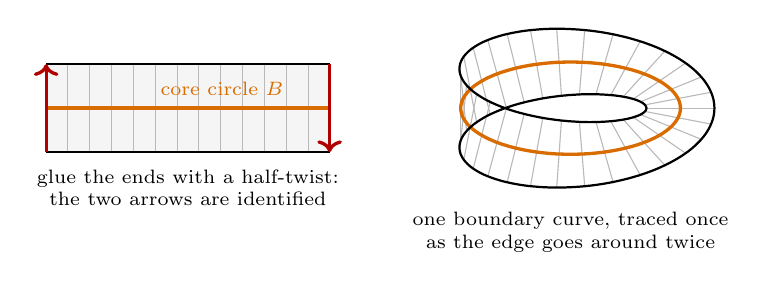
\begin{tikzpicture}[scale=0.9]
\fill[gray!8] (0,-0.62) rectangle (4.00,0.62);
\draw[gray!55] (0.30,-0.62) -- (0.30,0.62);
\draw[gray!55] (0.61,-0.62) -- (0.61,0.62);
\draw[gray!55] (0.92,-0.62) -- (0.92,0.62);
\draw[gray!55] (1.23,-0.62) -- (1.23,0.62);
\draw[gray!55] (1.54,-0.62) -- (1.54,0.62);
\draw[gray!55] (1.85,-0.62) -- (1.85,0.62);
\draw[gray!55] (2.15,-0.62) -- (2.15,0.62);
\draw[gray!55] (2.46,-0.62) -- (2.46,0.62);
\draw[gray!55] (2.77,-0.62) -- (2.77,0.62);
\draw[gray!55] (3.08,-0.62) -- (3.08,0.62);
\draw[gray!55] (3.39,-0.62) -- (3.39,0.62);
\draw[gray!55] (3.70,-0.62) -- (3.70,0.62);
\draw[thick] (0,0.62) -- (4.00,0.62); \draw[thick] (0,-0.62) -- (4.00,-0.62);
\draw[orange!85!black, very thick] (0,0) -- (4.00,0);
\draw[very thick, red!70!black, ->] (0,-0.62) -- (0,0.62); \draw[very thick, red!70!black, ->] (4.00,0.62) -- (4.00,-0.62);
\node[font=\scriptsize, align=center, anchor=north] at (2.00,-0.74) {glue the ends with a half-twist:\\ the two arrows are identified};
\node[orange!85!black, font=\scriptsize, anchor=south] at (2.48,0.04) {core circle $B$};
\draw[gray!55] (8.470,0.000) -- (8.607,0.000) -- (8.744,0.000) -- (8.881,0.000) -- (9.019,0.000) -- (9.156,0.000) -- (9.293,0.000) -- (9.430,0.000);
\draw[gray!55] (8.449,0.046) -- (8.583,0.072) -- (8.716,0.097) -- (8.849,0.123) -- (8.983,0.148) -- (9.116,0.174) -- (9.250,0.199) -- (9.383,0.225);
\draw[gray!55] (8.387,0.090) -- (8.510,0.140) -- (8.632,0.190) -- (8.755,0.240) -- (8.877,0.290) -- (9.000,0.340) -- (9.122,0.390) -- (9.245,0.440);
\draw[gray!55] (8.285,0.129) -- (8.390,0.201) -- (8.496,0.274) -- (8.601,0.346) -- (8.707,0.419) -- (8.812,0.491) -- (8.918,0.564) -- (9.023,0.636);
\draw[gray!55] (8.144,0.161) -- (8.228,0.254) -- (8.311,0.346) -- (8.395,0.438) -- (8.479,0.530) -- (8.563,0.622) -- (8.647,0.714) -- (8.731,0.806);
\draw[gray!55] (7.967,0.185) -- (8.027,0.293) -- (8.086,0.401) -- (8.145,0.510) -- (8.205,0.618) -- (8.264,0.726) -- (8.323,0.835) -- (8.383,0.943);
\draw[gray!55] (7.759,0.196) -- (7.793,0.317) -- (7.828,0.438) -- (7.862,0.559) -- (7.896,0.680) -- (7.930,0.800) -- (7.965,0.921) -- (7.999,1.042);
\draw[gray!55] (7.525,0.193) -- (7.535,0.323) -- (7.546,0.453) -- (7.557,0.583) -- (7.567,0.712) -- (7.578,0.842) -- (7.589,0.972) -- (7.599,1.102);
\draw[gray!55] (7.272,0.174) -- (7.262,0.310) -- (7.252,0.445) -- (7.243,0.580) -- (7.233,0.715) -- (7.224,0.850) -- (7.214,0.985) -- (7.204,1.120);
\draw[gray!55] (7.008,0.138) -- (6.983,0.275) -- (6.958,0.413) -- (6.933,0.550) -- (6.909,0.688) -- (6.884,0.826) -- (6.859,0.963) -- (6.834,1.101);
\draw[gray!55] (6.745,0.082) -- (6.711,0.219) -- (6.676,0.357) -- (6.642,0.495) -- (6.608,0.633) -- (6.574,0.770) -- (6.539,0.908) -- (6.505,1.046);
\draw[gray!55] (6.493,0.006) -- (6.456,0.143) -- (6.419,0.279) -- (6.382,0.416) -- (6.344,0.552) -- (6.307,0.688) -- (6.270,0.825) -- (6.232,0.961);
\draw[gray!55] (6.266,-0.088) -- (6.232,0.047) -- (6.197,0.181) -- (6.163,0.315) -- (6.129,0.450) -- (6.095,0.584) -- (6.060,0.719) -- (6.026,0.853);
\draw[gray!55] (6.075,-0.198) -- (6.049,-0.066) -- (6.023,0.066) -- (5.997,0.199) -- (5.971,0.331) -- (5.945,0.463) -- (5.919,0.596) -- (5.893,0.728);
\draw[gray!55] (5.933,-0.323) -- (5.919,-0.192) -- (5.905,-0.061) -- (5.891,0.070) -- (5.877,0.201) -- (5.863,0.332) -- (5.849,0.462) -- (5.835,0.593);
\draw[gray!55] (5.850,-0.456) -- (5.850,-0.326) -- (5.850,-0.195) -- (5.850,-0.065) -- (5.850,0.065) -- (5.850,0.195) -- (5.850,0.326) -- (5.850,0.456);
\draw[gray!55] (5.835,-0.593) -- (5.849,-0.462) -- (5.863,-0.332) -- (5.877,-0.201) -- (5.891,-0.070) -- (5.905,0.061) -- (5.919,0.192) -- (5.933,0.323);
\draw[gray!55] (5.893,-0.728) -- (5.919,-0.596) -- (5.945,-0.463) -- (5.971,-0.331) -- (5.997,-0.199) -- (6.023,-0.066) -- (6.049,0.066) -- (6.075,0.198);
\draw[gray!55] (6.026,-0.853) -- (6.060,-0.719) -- (6.095,-0.584) -- (6.129,-0.450) -- (6.163,-0.315) -- (6.197,-0.181) -- (6.232,-0.047) -- (6.266,0.088);
\draw[gray!55] (6.232,-0.961) -- (6.270,-0.825) -- (6.307,-0.688) -- (6.344,-0.552) -- (6.382,-0.416) -- (6.419,-0.279) -- (6.456,-0.143) -- (6.493,-0.006);
\draw[gray!55] (6.505,-1.046) -- (6.539,-0.908) -- (6.574,-0.770) -- (6.608,-0.633) -- (6.642,-0.495) -- (6.676,-0.357) -- (6.711,-0.219) -- (6.745,-0.082);
\draw[gray!55] (6.834,-1.101) -- (6.859,-0.963) -- (6.884,-0.826) -- (6.909,-0.688) -- (6.933,-0.550) -- (6.958,-0.413) -- (6.983,-0.275) -- (7.008,-0.138);
\draw[gray!55] (7.204,-1.120) -- (7.214,-0.985) -- (7.224,-0.850) -- (7.233,-0.715) -- (7.243,-0.580) -- (7.252,-0.445) -- (7.262,-0.310) -- (7.272,-0.174);
\draw[gray!55] (7.599,-1.102) -- (7.589,-0.972) -- (7.578,-0.842) -- (7.567,-0.712) -- (7.557,-0.583) -- (7.546,-0.453) -- (7.535,-0.323) -- (7.525,-0.193);
\draw[gray!55] (7.999,-1.042) -- (7.965,-0.921) -- (7.930,-0.800) -- (7.896,-0.680) -- (7.862,-0.559) -- (7.828,-0.438) -- (7.793,-0.317) -- (7.759,-0.196);
\draw[gray!55] (8.383,-0.943) -- (8.323,-0.835) -- (8.264,-0.726) -- (8.205,-0.618) -- (8.145,-0.510) -- (8.086,-0.401) -- (8.027,-0.293) -- (7.967,-0.185);
\draw[gray!55] (8.731,-0.806) -- (8.647,-0.714) -- (8.563,-0.622) -- (8.479,-0.530) -- (8.395,-0.438) -- (8.311,-0.346) -- (8.228,-0.254) -- (8.144,-0.161);
\draw[gray!55] (9.023,-0.636) -- (8.918,-0.564) -- (8.812,-0.491) -- (8.707,-0.419) -- (8.601,-0.346) -- (8.496,-0.274) -- (8.390,-0.201) -- (8.285,-0.129);
\draw[gray!55] (9.245,-0.440) -- (9.122,-0.390) -- (9.000,-0.340) -- (8.877,-0.290) -- (8.755,-0.240) -- (8.632,-0.190) -- (8.510,-0.140) -- (8.387,-0.090);
\draw[gray!55] (9.383,-0.225) -- (9.250,-0.199) -- (9.116,-0.174) -- (8.983,-0.148) -- (8.849,-0.123) -- (8.716,-0.097) -- (8.583,-0.072) -- (8.449,-0.046);
\draw[orange!85!black, very thick] (8.950,0.000) -- (8.949,0.026) -- (8.945,0.051) -- (8.939,0.077) -- (8.931,0.102) -- (8.920,0.128) -- (8.907,0.153) -- (8.891,0.178) -- (8.873,0.202) -- (8.853,0.227) -- (8.831,0.251) -- (8.806,0.274) -- (8.779,0.297) -- (8.750,0.320) -- (8.719,0.342) -- (8.686,0.364) -- (8.650,0.385) -- (8.613,0.405) -- (8.574,0.425) -- (8.533,0.444) -- (8.491,0.463) -- (8.446,0.480) -- (8.400,0.497) -- (8.353,0.514) -- (8.304,0.529) -- (8.253,0.544) -- (8.201,0.557) -- (8.148,0.570) -- (8.094,0.582) -- (8.039,0.593) -- (7.983,0.603) -- (7.925,0.612) -- (7.867,0.621) -- (7.809,0.628) -- (7.749,0.634) -- (7.689,0.640) -- (7.629,0.644) -- (7.568,0.647) -- (7.507,0.649) -- (7.446,0.651) -- (7.385,0.651) -- (7.323,0.650) -- (7.262,0.648) -- (7.201,0.646) -- (7.141,0.642) -- (7.081,0.637) -- (7.021,0.631) -- (6.962,0.624) -- (6.904,0.617) -- (6.846,0.608) -- (6.789,0.598) -- (6.733,0.588) -- (6.679,0.576) -- (6.625,0.564) -- (6.573,0.550) -- (6.521,0.536) -- (6.472,0.521) -- (6.423,0.506) -- (6.377,0.489) -- (6.331,0.472) -- (6.288,0.453) -- (6.246,0.435) -- (6.206,0.415) -- (6.168,0.395) -- (6.132,0.374) -- (6.098,0.353) -- (6.065,0.331) -- (6.035,0.309) -- (6.007,0.286) -- (5.982,0.262) -- (5.958,0.239) -- (5.937,0.215) -- (5.918,0.190) -- (5.901,0.165) -- (5.886,0.140) -- (5.874,0.115) -- (5.865,0.090) -- (5.858,0.064) -- (5.853,0.039) -- (5.850,0.013) -- (5.850,-0.013) -- (5.853,-0.039) -- (5.858,-0.064) -- (5.865,-0.090) -- (5.874,-0.115) -- (5.886,-0.140) -- (5.901,-0.165) -- (5.918,-0.190) -- (5.937,-0.215) -- (5.958,-0.239) -- (5.982,-0.262) -- (6.007,-0.286) -- (6.035,-0.309) -- (6.065,-0.331) -- (6.098,-0.353) -- (6.132,-0.374) -- (6.168,-0.395) -- (6.206,-0.415) -- (6.246,-0.435) -- (6.288,-0.453) -- (6.331,-0.472) -- (6.377,-0.489) -- (6.423,-0.506) -- (6.472,-0.521) -- (6.521,-0.536) -- (6.573,-0.550) -- (6.625,-0.564) -- (6.679,-0.576) -- (6.733,-0.588) -- (6.789,-0.598) -- (6.846,-0.608) -- (6.904,-0.617) -- (6.962,-0.624) -- (7.021,-0.631) -- (7.081,-0.637) -- (7.141,-0.642) -- (7.201,-0.646) -- (7.262,-0.648) -- (7.323,-0.650) -- (7.385,-0.651) -- (7.446,-0.651) -- (7.507,-0.649) -- (7.568,-0.647) -- (7.629,-0.644) -- (7.689,-0.640) -- (7.749,-0.634) -- (7.809,-0.628) -- (7.867,-0.621) -- (7.925,-0.612) -- (7.983,-0.603) -- (8.039,-0.593) -- (8.094,-0.582) -- (8.148,-0.570) -- (8.201,-0.557) -- (8.253,-0.544) -- (8.304,-0.529) -- (8.353,-0.514) -- (8.400,-0.497) -- (8.446,-0.480) -- (8.491,-0.463) -- (8.533,-0.444) -- (8.574,-0.425) -- (8.613,-0.405) -- (8.650,-0.385) -- (8.686,-0.364) -- (8.719,-0.342) -- (8.750,-0.320) -- (8.779,-0.297) -- (8.806,-0.274) -- (8.831,-0.251) -- (8.853,-0.227) -- (8.873,-0.202) -- (8.891,-0.178) -- (8.907,-0.153) -- (8.920,-0.128) -- (8.931,-0.102) -- (8.939,-0.077) -- (8.945,-0.051) -- (8.949,-0.026) -- (8.950,-0.000);
\draw[thick] (9.430,0.000) -- (9.428,0.043) -- (9.423,0.085) -- (9.415,0.127) -- (9.403,0.170) -- (9.388,0.211) -- (9.370,0.253) -- (9.349,0.294) -- (9.324,0.335) -- (9.297,0.375) -- (9.266,0.415) -- (9.232,0.454) -- (9.195,0.492) -- (9.156,0.530) -- (9.114,0.567) -- (9.069,0.603) -- (9.021,0.638) -- (8.971,0.672) -- (8.918,0.705) -- (8.863,0.737) -- (8.806,0.768) -- (8.747,0.798) -- (8.685,0.827) -- (8.622,0.855) -- (8.558,0.881) -- (8.491,0.906) -- (8.423,0.930) -- (8.354,0.952) -- (8.283,0.973) -- (8.212,0.993) -- (8.139,1.011) -- (8.066,1.028) -- (7.992,1.044) -- (7.917,1.058) -- (7.842,1.071) -- (7.767,1.082) -- (7.691,1.092) -- (7.616,1.100) -- (7.540,1.107) -- (7.465,1.112) -- (7.391,1.116) -- (7.317,1.119) -- (7.243,1.120) -- (7.171,1.120) -- (7.099,1.119) -- (7.028,1.116) -- (6.959,1.112) -- (6.891,1.106) -- (6.824,1.100) -- (6.759,1.092) -- (6.695,1.083) -- (6.633,1.072) -- (6.573,1.061) -- (6.515,1.048) -- (6.458,1.035) -- (6.404,1.020) -- (6.352,1.004) -- (6.302,0.988) -- (6.254,0.970) -- (6.209,0.952) -- (6.166,0.933) -- (6.126,0.913) -- (6.088,0.892) -- (6.052,0.870) -- (6.020,0.849) -- (5.989,0.826) -- (5.962,0.803) -- (5.937,0.779) -- (5.915,0.755) -- (5.895,0.731) -- (5.878,0.706) -- (5.864,0.681) -- (5.852,0.656) -- (5.843,0.630) -- (5.837,0.604) -- (5.833,0.579) -- (5.832,0.553) -- (5.833,0.527) -- (5.837,0.501) -- (5.844,0.475) -- (5.852,0.450) -- (5.864,0.424) -- (5.877,0.399) -- (5.893,0.374) -- (5.911,0.349) -- (5.932,0.324) -- (5.954,0.300) -- (5.978,0.276) -- (6.005,0.253) -- (6.033,0.229) -- (6.063,0.207) -- (6.095,0.185) -- (6.129,0.163) -- (6.164,0.142) -- (6.200,0.121) -- (6.239,0.101) -- (6.278,0.082) -- (6.319,0.063) -- (6.361,0.045) -- (6.404,0.027) -- (6.448,0.010) -- (6.493,-0.006) -- (6.539,-0.022) -- (6.585,-0.037) -- (6.632,-0.051) -- (6.680,-0.065) -- (6.729,-0.077) -- (6.778,-0.090) -- (6.827,-0.101) -- (6.876,-0.112) -- (6.926,-0.122) -- (6.976,-0.132) -- (7.026,-0.141) -- (7.075,-0.149) -- (7.125,-0.156) -- (7.175,-0.163) -- (7.224,-0.169) -- (7.273,-0.175) -- (7.322,-0.179) -- (7.370,-0.184) -- (7.418,-0.187) -- (7.465,-0.190) -- (7.512,-0.193) -- (7.558,-0.195) -- (7.603,-0.196) -- (7.647,-0.197) -- (7.691,-0.197) -- (7.734,-0.196) -- (7.776,-0.196) -- (7.817,-0.194) -- (7.857,-0.192) -- (7.895,-0.190) -- (7.933,-0.187) -- (7.970,-0.184) -- (8.006,-0.181) -- (8.040,-0.177) -- (8.074,-0.172) -- (8.106,-0.168) -- (8.137,-0.163) -- (8.166,-0.157) -- (8.195,-0.152) -- (8.222,-0.146) -- (8.247,-0.139) -- (8.272,-0.133) -- (8.295,-0.126) -- (8.316,-0.119) -- (8.337,-0.112) -- (8.356,-0.104) -- (8.373,-0.097) -- (8.389,-0.089) -- (8.404,-0.081) -- (8.417,-0.073) -- (8.429,-0.064) -- (8.439,-0.056) -- (8.448,-0.048) -- (8.455,-0.039) -- (8.461,-0.030) -- (8.465,-0.022) -- (8.468,-0.013) -- (8.470,-0.004) -- (8.470,0.004) -- (8.468,0.013) -- (8.465,0.022) -- (8.461,0.030) -- (8.455,0.039) -- (8.448,0.048) -- (8.439,0.056) -- (8.429,0.064) -- (8.417,0.073) -- (8.404,0.081) -- (8.389,0.089) -- (8.373,0.097) -- (8.356,0.104) -- (8.337,0.112) -- (8.316,0.119) -- (8.295,0.126) -- (8.272,0.133) -- (8.247,0.139) -- (8.222,0.146) -- (8.195,0.152) -- (8.166,0.157) -- (8.137,0.163) -- (8.106,0.168) -- (8.074,0.172) -- (8.040,0.177) -- (8.006,0.181) -- (7.970,0.184) -- (7.933,0.187) -- (7.895,0.190) -- (7.857,0.192) -- (7.817,0.194) -- (7.776,0.196) -- (7.734,0.196) -- (7.691,0.197) -- (7.647,0.197) -- (7.603,0.196) -- (7.558,0.195) -- (7.512,0.193) -- (7.465,0.190) -- (7.418,0.187) -- (7.370,0.184) -- (7.322,0.179) -- (7.273,0.175) -- (7.224,0.169) -- (7.175,0.163) -- (7.125,0.156) -- (7.075,0.149) -- (7.026,0.141) -- (6.976,0.132) -- (6.926,0.122) -- (6.876,0.112) -- (6.827,0.101) -- (6.778,0.090) -- (6.729,0.077) -- (6.680,0.065) -- (6.632,0.051) -- (6.585,0.037) -- (6.539,0.022) -- (6.493,0.006) -- (6.448,-0.010) -- (6.404,-0.027) -- (6.361,-0.045) -- (6.319,-0.063) -- (6.278,-0.082) -- (6.239,-0.101) -- (6.200,-0.121) -- (6.164,-0.142) -- (6.129,-0.163) -- (6.095,-0.185) -- (6.063,-0.207) -- (6.033,-0.229) -- (6.005,-0.253) -- (5.978,-0.276) -- (5.954,-0.300) -- (5.932,-0.324) -- (5.911,-0.349) -- (5.893,-0.374) -- (5.877,-0.399) -- (5.864,-0.424) -- (5.852,-0.450) -- (5.844,-0.475) -- (5.837,-0.501) -- (5.833,-0.527) -- (5.832,-0.553) -- (5.833,-0.579) -- (5.837,-0.604) -- (5.843,-0.630) -- (5.852,-0.656) -- (5.864,-0.681) -- (5.878,-0.706) -- (5.895,-0.731) -- (5.915,-0.755) -- (5.937,-0.779) -- (5.962,-0.803) -- (5.989,-0.826) -- (6.020,-0.849) -- (6.052,-0.870) -- (6.088,-0.892) -- (6.126,-0.913) -- (6.166,-0.933) -- (6.209,-0.952) -- (6.254,-0.970) -- (6.302,-0.988) -- (6.352,-1.004) -- (6.404,-1.020) -- (6.458,-1.035) -- (6.515,-1.048) -- (6.573,-1.061) -- (6.633,-1.072) -- (6.695,-1.083) -- (6.759,-1.092) -- (6.824,-1.100) -- (6.891,-1.106) -- (6.959,-1.112) -- (7.028,-1.116) -- (7.099,-1.119) -- (7.171,-1.120) -- (7.243,-1.120) -- (7.317,-1.119) -- (7.391,-1.116) -- (7.465,-1.112) -- (7.540,-1.107) -- (7.616,-1.100) -- (7.691,-1.092) -- (7.767,-1.082) -- (7.842,-1.071) -- (7.917,-1.058) -- (7.992,-1.044) -- (8.066,-1.028) -- (8.139,-1.011) -- (8.212,-0.993) -- (8.283,-0.973) -- (8.354,-0.952) -- (8.423,-0.930) -- (8.491,-0.906) -- (8.558,-0.881) -- (8.622,-0.855) -- (8.685,-0.827) -- (8.747,-0.798) -- (8.806,-0.768) -- (8.863,-0.737) -- (8.918,-0.705) -- (8.971,-0.672) -- (9.021,-0.638) -- (9.069,-0.603) -- (9.114,-0.567) -- (9.156,-0.530) -- (9.195,-0.492) -- (9.232,-0.454) -- (9.266,-0.415) -- (9.297,-0.375) -- (9.324,-0.335) -- (9.349,-0.294) -- (9.370,-0.253) -- (9.388,-0.211) -- (9.403,-0.170) -- (9.415,-0.127) -- (9.423,-0.085) -- (9.428,-0.043) -- (9.430,-0.000);
\node[font=\scriptsize, align=center] at (7.40,-1.75) {one boundary curve, traced once\\ as the edge goes around twice};
\end{tikzpicture}
\end{center}

Left: the strip $[0, 1] \times (-1, 1)$, ruled by its fibres, with the core circle in orange; glue the two ends with a half-twist, matching the arrows. Right: the band itself. Each grey segment is a fibre, lying over one point of the orange core circle, and the boundary is a single curve.

% ============================================================
% Lecture 13 (Wed Sep 30, 2026)
% ============================================================

\subsection{When Is a Submersion a Fibration?}\label{sub:ehresmann}

\textit{Lecture 13 (Wed Sep 30). Uribe opened with the answer to the question left open in Lecture~12 --- ``I didn't know the answer right away. I thought the answer was no, and in fact the answer is no. But there's a partial yes.''}

\begin{thmbox}[Ehresmann's Theorem]\thmlabel{thm:ehresmann}
Let $\pi : E \to B$ be a surjective submersion which is \emph{proper}: the preimage of every compact set is compact. If $B$ is connected, then $\pi$ is a fibration.
\end{thmbox}

\begin{proof}[Proof (to be filled)]
Stated in Lecture~13, not proved: the proof uses connections, which the course does not cover. To be filled.
\end{proof}

\textit{Status.} Stated in Lecture~13, not proved: ``we don't have time to do the proof, and it uses material that we're not going to cover called connections.'' Uribe first recalled the case of a compact fibre, then the general statement for proper maps, which is the form given here. The intuition: a connection lets one lift a path from $b$ to $b'$ in the base to paths in $E$, and flow the fibre over $b$ onto the fibre over $b'$; properness is what lets the flow run for as long as needed, so that it identifies the fibres not just one at a time but over a whole neighbourhood --- a local trivialization. The transcript renders the name as ``Aristotle''; it is Ehresmann.

\begin{exbox}[All Fibres Diffeomorphic but Not a Fibration]\exlabel{ex:ehresmann-counter}
Let
\[
E = \big\{ (x, y, t) \in \mathbb{R}^3 : (x, y) \ne (0, 0), \ \text{and } (x, y) \ne (t, 0) \text{ if } t \ne 0, \ (x, y) \ne (1, 0) \text{ if } t = 0 \big\},
\]
and $\pi(x, y, t) = t$. Then $\pi : E \to \mathbb{R}$ is a surjective submersion, and every fibre is the plane minus two points:
\[
\pi^{-1}(t) \cong \begin{cases} \mathbb{R}^2 \setminus \{(0,0), (t,0)\}, & t \ne 0, \\ \mathbb{R}^2 \setminus \{(0,0), (1,0)\}, & t = 0, \end{cases}
\]
all diffeomorphic to one another. But $\pi$ is not a fibration.
\end{exbox}

\textit{Status.} Found for Uribe by ChatGPT, which reported that a human had posted it on a mathematics forum; given in lecture as a picture, without proof. \textit{(Completion.)} $E$ is open in $\mathbb{R}^3$: its complement is the $t$-axis $\{(0,0,t)\}$, together with the line $\{(t, 0, t)\}$ and the single point $(1, 0, 0)$, a closed set. So $\pi$ is the restriction of a projection to an open set, hence a submersion (Example~\ref{ex:projection-submersion}), and it is onto. Any two copies of the plane with two points removed are diffeomorphic by an affine map. That $\pi$ is not a fibration is stated, not proved, here. Uribe's intuition: as $t \to 0$ the missing point $(t, 0)$ ``is colliding with $(0,0)$'', while over $t = 0$ the second missing point sits away at $(1, 0)$. He added that the example is subtler than it looks: with lines in place of planes the corresponding map would be locally trivial, and ``it's the fact that you have [a] fundamental group that messes things up.''

\begin{center}
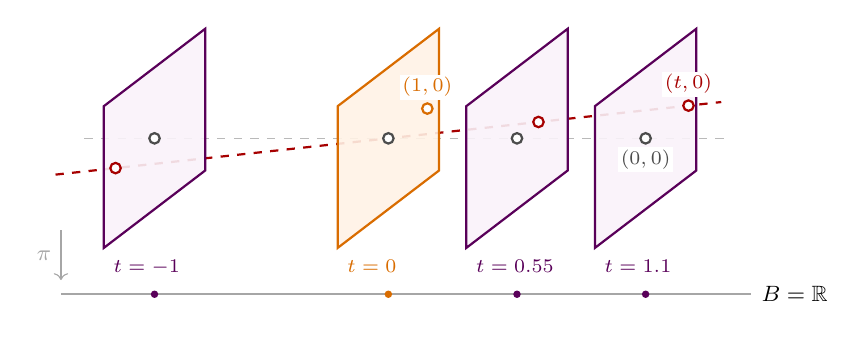
\begin{tikzpicture}[scale=0.9]
\draw[gray!55, dashed] (-4.290,0.000) -- (4.785,0.000);
\draw[red!65!black, dashed, thick] (-4.697,-0.512) -- (4.697,0.512);
\draw[violet!70!black, thick, fill=violet!5, fill opacity=0.9] (-4.015,-1.546) -- (-2.585,-0.454) -- (-2.585,1.546) -- (-4.015,0.454) -- cycle;
\draw[gray!60!black, fill=white, thick] (-3.300,0.000) circle (2.1pt);
\draw[red!65!black, fill=white, thick] (-3.850,-0.420) circle (2.1pt);
\node[font=\scriptsize, text=violet!70!black, anchor=north west] at (-4.015,-1.586) {$t = -1$};
\draw[orange!85!black, thick, fill=orange!10, fill opacity=0.9] (-0.715,-1.546) -- (0.715,-0.454) -- (0.715,1.546) -- (-0.715,0.454) -- cycle;
\draw[gray!60!black, fill=white, thick] (0.000,0.000) circle (2.1pt);
\draw[orange!85!black, fill=white, thick] (0.550,0.420) circle (2.1pt);
\node[font=\scriptsize, text=orange!85!black, anchor=north west] at (-0.715,-1.586) {$t = 0$};
\draw[violet!70!black, thick, fill=violet!5, fill opacity=0.9] (1.100,-1.546) -- (2.530,-0.454) -- (2.530,1.546) -- (1.100,0.454) -- cycle;
\draw[gray!60!black, fill=white, thick] (1.815,0.000) circle (2.1pt);
\draw[red!65!black, fill=white, thick] (2.118,0.231) circle (2.1pt);
\node[font=\scriptsize, text=violet!70!black, anchor=north west] at (1.100,-1.586) {$t = 0.55$};
\draw[violet!70!black, thick, fill=violet!5, fill opacity=0.9] (2.915,-1.546) -- (4.345,-0.454) -- (4.345,1.546) -- (2.915,0.454) -- cycle;
\draw[gray!60!black, fill=white, thick] (3.630,0.000) circle (2.1pt);
\draw[red!65!black, fill=white, thick] (4.235,0.462) circle (2.1pt);
\node[font=\scriptsize, text=violet!70!black, anchor=north west] at (2.915,-1.586) {$t = 1.1$};
\node[orange!85!black, font=\scriptsize, anchor=south, fill=white, inner sep=1pt] at (0.550,0.540) {$(1,0)$};
\node[red!65!black, font=\scriptsize, anchor=south, fill=white, inner sep=1pt] at (4.235,0.582) {$(t,0)$};
\node[gray!60!black, font=\scriptsize, anchor=north, fill=white, inner sep=1pt] at (3.630,-0.120) {$(0,0)$};
\draw[thick, gray!70] (-4.62,-2.2) -- (5.12,-2.2) node[right, font=\footnotesize, text=black] {$B = \mathbb{R}$};
\fill[violet!70!black] (-3.300,-2.2) circle (1.5pt);
\fill[orange!85!black] (0.000,-2.2) circle (1.5pt);
\fill[violet!70!black] (1.815,-2.2) circle (1.5pt);
\fill[violet!70!black] (3.630,-2.2) circle (1.5pt);
\draw[->, gray!70] (-4.62,-1.3) -- node[left, font=\footnotesize] {$\pi$} (-4.62,-2.0);
\end{tikzpicture}
\end{center}

The fibres over a few values of $t$. The origin, grey, is missing from every fibre, and the missing points $(t, 0)$, red, lie on a line --- dashed --- which meets the line of origins exactly at $t = 0$: the collision. Over $t = 0$ (orange) the second missing point is $(1, 0)$, off that line. Each fibre on its own is a plane minus two points; what fails is the way they fit together near $t = 0$.

\textbf{Transcription note.} Page~35 of the handwritten notes labels the second missing point over $t = 0$ as $(1, 1)$; it is $(1, 0)$.

\subsection{Sections and Local Sections}\label{sub:local-sections}

\textit{From Assignment~4, Problem~4, whose hint --- ``declare that $\Phi_i \circ s_i$ includes $U_i \to U_i \times \{1\}$, and extend the definition of $\Phi_i$ by equivariance'' --- contains a general principle: local trivializations and local sections are two descriptions of the same thing.}

\begin{defbox}[Section]\deflabel{def:section}
Let $\pi : E \to B$ be a fibration. A \textbf{section} of $\pi$ is a smooth map $s : B \to E$ with $\pi \circ s = \mathrm{id}_B$: ``if you first go up and then down, you get the identity on the base.'' It picks, smoothly in $b$, one point $s(b)$ of each fibre $\pi^{-1}(b)$.
\leeref{Ch.~10, \emph{Sections of Vector Bundles}}
\end{defbox}

\begin{center}
\begin{tikzcd}[row sep=3.2em]
E \arrow[d, shift right=0.9ex, "\pi"'] \\
B \arrow[u, shift right=0.9ex, "s"']
\end{tikzcd}
\qquad
\raisebox{1.6em}{$\pi \circ s = \mathrm{id}_B$}
\end{center}

A section goes up, the projection comes down, and the round trip is the identity on the base.

\begin{center}
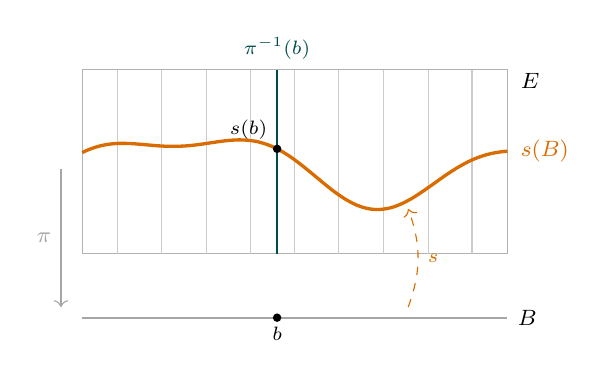
\begin{tikzpicture}[scale=0.9]
\draw[gray!60] (0,0) rectangle (6,2.6); \node[font=\footnotesize, anchor=south west] at (6.05,2.2) {$E$};
\draw[gray!40] (0.50,0) -- (0.50,2.6);
\draw[gray!40] (1.12,0) -- (1.12,2.6);
\draw[gray!40] (1.75,0) -- (1.75,2.6);
\draw[gray!40] (2.38,0) -- (2.38,2.6);
\draw[gray!40] (3.00,0) -- (3.00,2.6);
\draw[gray!40] (3.62,0) -- (3.62,2.6);
\draw[gray!40] (4.25,0) -- (4.25,2.6);
\draw[gray!40] (4.88,0) -- (4.88,2.6);
\draw[gray!40] (5.50,0) -- (5.50,2.6);
\draw[orange!85!black, very thick] (0.000,1.430) -- (0.050,1.454) -- (0.101,1.475) -- (0.151,1.494) -- (0.202,1.510) -- (0.252,1.524) -- (0.303,1.535) -- (0.353,1.544) -- (0.403,1.551) -- (0.454,1.556) -- (0.504,1.559) -- (0.555,1.560) -- (0.605,1.560) -- (0.655,1.558) -- (0.706,1.556) -- (0.756,1.552) -- (0.807,1.548) -- (0.857,1.544) -- (0.908,1.539) -- (0.958,1.535) -- (1.008,1.530) -- (1.059,1.526) -- (1.109,1.523) -- (1.160,1.520) -- (1.210,1.519) -- (1.261,1.518) -- (1.311,1.518) -- (1.361,1.519) -- (1.412,1.521) -- (1.462,1.524) -- (1.513,1.528) -- (1.563,1.533) -- (1.613,1.539) -- (1.664,1.546) -- (1.714,1.553) -- (1.765,1.560) -- (1.815,1.568) -- (1.866,1.575) -- (1.916,1.583) -- (1.966,1.589) -- (2.017,1.596) -- (2.067,1.601) -- (2.118,1.605) -- (2.168,1.608) -- (2.218,1.609) -- (2.269,1.608) -- (2.319,1.605) -- (2.370,1.600) -- (2.420,1.593) -- (2.471,1.584) -- (2.521,1.571) -- (2.571,1.556) -- (2.622,1.539) -- (2.672,1.519) -- (2.723,1.496) -- (2.773,1.470) -- (2.824,1.442) -- (2.874,1.412) -- (2.924,1.379) -- (2.975,1.344) -- (3.025,1.307) -- (3.076,1.269) -- (3.126,1.229) -- (3.176,1.188) -- (3.227,1.147) -- (3.277,1.105) -- (3.328,1.063) -- (3.378,1.021) -- (3.429,0.979) -- (3.479,0.939) -- (3.529,0.899) -- (3.580,0.862) -- (3.630,0.826) -- (3.681,0.792) -- (3.731,0.761) -- (3.782,0.733) -- (3.832,0.707) -- (3.882,0.685) -- (3.933,0.666) -- (3.983,0.651) -- (4.034,0.639) -- (4.084,0.631) -- (4.134,0.627) -- (4.185,0.626) -- (4.235,0.630) -- (4.286,0.637) -- (4.336,0.647) -- (4.387,0.661) -- (4.437,0.678) -- (4.487,0.699) -- (4.538,0.722) -- (4.588,0.748) -- (4.639,0.776) -- (4.689,0.806) -- (4.739,0.838) -- (4.790,0.872) -- (4.840,0.906) -- (4.891,0.942) -- (4.941,0.977) -- (4.992,1.014) -- (5.042,1.049) -- (5.092,1.085) -- (5.143,1.120) -- (5.193,1.153) -- (5.244,1.186) -- (5.294,1.217) -- (5.345,1.246) -- (5.395,1.274) -- (5.445,1.300) -- (5.496,1.324) -- (5.546,1.345) -- (5.597,1.365) -- (5.647,1.382) -- (5.697,1.397) -- (5.748,1.411) -- (5.798,1.422) -- (5.849,1.431) -- (5.899,1.439) -- (5.950,1.445) -- (6.000,1.450); \node[orange!85!black, font=\footnotesize, anchor=west] at (6.05,1.450) {$s(B)$};
\draw[teal!60!black, thick] (2.75,0) -- (2.75,2.6) node[above, font=\scriptsize] {$\pi^{-1}(b)$};
\fill (2.750,1.482) circle (1.7pt) node[font=\scriptsize, anchor=south east] {$s(b)$};
\draw[thick, gray!70] (0,-0.9) -- (6,-0.9) node[right, font=\footnotesize, text=black] {$B$};
\fill (2.75,-0.9) circle (1.7pt) node[below, font=\scriptsize] {$b$};
\draw[->, gray!70] (-0.3,1.2) -- node[left, font=\footnotesize] {$\pi$} (-0.3,-0.75);
\draw[->, dashed, orange!85!black] (4.6,-0.75) to[bend right=20] node[right, font=\scriptsize] {$s$} (4.600,0.634);
\end{tikzpicture}
\end{center}

The cartoon of a section. The fibration is drawn as a box over its base, with fibres vertical; a section is a graph over the base, meeting every fibre exactly once --- at $s(b)$ in the fibre over $b$ --- so its image $s(B)$ is ``a copy of $B$'' inside $E$.

\begin{defbox}[Local Section]\deflabel{def:local-section}
Let $\pi : E \to B$ be smooth and $U \subseteq B$ open. A \textbf{local section} of $\pi$ over $U$ is a smooth map $s : U \to E$ with $\pi \circ s = \mathrm{id}_U$.
\leeref{Ch.~10, \emph{Local and Global Sections of Vector Bundles}}
\end{defbox}

A section in the sense of Definition~\ref{def:section} is a local section over $U = B$; to stress the difference, it is also called a \emph{global} section.

\begin{propbox}[Local Trivializations Give Local Sections]\thmlabel{prop:trivialization-section}
Let $\pi : E \to B$ be a fibration with fibre $F$, and $\phi : \pi^{-1}(U) \to U \times F$ a local trivialization. For every $f_0 \in F$, the map $s(u) = \phi^{-1}(u, f_0)$ is a local section over $U$.
\end{propbox}

\begin{proof}
\textit{(Not from lecture; filled in.)} $s$ is smooth, a composite of $u \mapsto (u, f_0)$ and the diffeomorphism $\phi^{-1}$; and $\pi(s(u)) = \mathrm{pr}_1\big(\phi(s(u))\big) = \mathrm{pr}_1(u, f_0) = u$, because $\pi = \mathrm{pr}_1 \circ \phi$.
\end{proof}

\section{Immersions}\label{sec:immersions}

\roadmark{Stage: maps}{The maps with injective differentials: locally inclusions, globally more subtle.}

\textit{References: Lee Ch.~4. Lecture 13.} The third special type of map, dual to the submersions of \ref{sec:submersions}: the differential is injective instead of surjective, and the local model is an inclusion instead of a projection.

\subsection{Immersions}\label{sub:immersions}

\textit{Lecture 13. ``Next class of special maps'': Lecture~10 listed immersions among the special types of map, and the definition has been on record since (Definition~\ref{def:submersion}); Lecture~13 is where they were first treated seriously, after the tangent bundle (\ref{sec:tangent-bundle}).}

\begin{defbox}[Immersions]\deflabel{def:immersion-lecture}
Let $F : M \to N$ be smooth, with $\dim M = m$ and $\dim N = n$. $F$ is an \textbf{immersion at $p$} if $F_{*p} : T_pM \to T_{F(p)}N$ is injective --- which forces $m \le n$, since an injective linear map cannot lower dimension --- and an \textbf{immersion} if it is an immersion at every point. ``Go from a lower-dimensional manifold to a bigger one.''
\leeref{Ch.~4, \emph{Immersions}}
\end{defbox}

\begin{thmbox}[Local Normal Form for Immersions]\thmlabel{thm:immersion-normal-form}
Let $F : M \to N$ be an immersion at $p$, with $\dim M = m \le n = \dim N$. Then there are charts $(U, \varphi = (x^1, \ldots, x^m))$ at $p$ and $(V, \psi = (y^1, \ldots, y^n))$ at $F(p)$ with $F(U) \subseteq V$ in which the coordinate representation $\tilde F = \psi \circ F \circ \varphi^{-1}$ is the standard inclusion:
\[
\tilde F(r^1, \ldots, r^m) = (r^1, \ldots, r^m, \underbrace{0, \ldots, 0}_{n - m}) .
\]
\leeref{Theorem 4.12, the rank theorem}
\end{thmbox}

\begin{proof}[Proof (Lecture~14)]
The steps are the lecture's, in the lecture's order; sentences marked \textit{(Completion.)} fill in details. The first half runs as for submersions (Theorem~\ref{thm:submersion-normal-form}); the new step is that here the chart on $N$ changes too.

\emph{1. Start with any coordinates.} Take charts $(U_0, \varphi_0 = (x^1, \ldots, x^m))$ at $p$ and $(V_0, \psi = (y^1, \ldots, y^n))$ at $F(p)$ with $F(U_0) \subseteq V_0$, shrinking $U_0$ if necessary, and write $F^j = y^j \circ F$.

\emph{2. The Jacobian is taller than wide.} $J = \big[\partial F^j/\partial x^i(p)\big]$ is the matrix of $F_{*p}$ (Theorem~\ref{lem:differential-matrix}): $n$ rows and $m$ columns, ``fewer columns than rows.'' $F_{*p}$ is injective, so $J$ has rank $m$: it has $m$ linearly independent row vectors.

\emph{3. Relabel the $y$'s.} Reordering the coordinates of $\psi$ --- again a smooth chart, as in step~4 of the proof of Theorem~\ref{thm:submersion-normal-form} --- we may assume the top $m \times m$ block $A$ of $J$ is invertible.

\emph{4. The first $m$ components of $F$ are coordinates on $M$.} $A$ is the Jacobian at $p$, in the $x$-coordinates, of the map $U_0 \to \mathbb{R}^m$ that sends $q$ to the first $m$ components $\big(F^1(q), \ldots, F^m(q)\big)$ (Proposition~\ref{prop:upstairs-downstairs}). It is invertible, so by the inverse function theorem (Theorem~\ref{thm:inverse-function}) --- ``I always say implicit, but in this case I want the inverse function theorem'' --- this map is a local diffeomorphism near $p$, and, possibly after shrinking $U_0$ to some $U \ni p$, it is a chart:
\[
\tilde\varphi = \big(F^1, \ldots, F^m\big)\big|_U : U \longrightarrow \tilde\varphi(U) \subseteq \mathbb{R}^m .
\]
\textit{(Completion.)} As in step~8 of the proof of Theorem~\ref{thm:submersion-normal-form}: the inverse function theorem gives an open $W \ni \varphi_0(p)$ on which $\tilde\varphi \circ \varphi_0^{-1}$ is a diffeomorphism onto an open set; put $U = \varphi_0^{-1}(W)$; then $\tilde\varphi$ maps $U$ diffeomorphically onto an open set, and is a chart by Lemma~\ref{lem:diffeo-chart}.

\emph{5. In the new chart, $F$ is a graph.} Let $\hat F = \psi \circ F \circ \tilde\varphi^{-1} : \tilde\varphi(U) \to \psi(V_0)$. By the definition of $\tilde\varphi$, the first $m$ components of $\hat F(r)$ are $F^i(\tilde\varphi^{-1}(r)) = r^i$, so
\[
\hat F(r) = \big(r, \ G^1(r), \ldots, G^{n-m}(r)\big), \qquad G^k = F^{m+k} \circ \tilde\varphi^{-1} ,
\]
with $G = (G^1, \ldots, G^{n-m})$ smooth on $\tilde\varphi(U)$. ``I don't get zeros yet. I get something'': $\hat F$ is the graph of $G$ over $\tilde\varphi(U)$.

\emph{6. Straighten the graph.} ``You can always straighten out a graph to make it zero.'' Define new coordinates on $N$ by keeping the first $m$ and shifting the rest: ``I always mess up my indices \ldots\ so I'm going to cheat''
\[
\tilde y^i = y^i \quad (1 \le i \le m), \qquad \tilde y^i = y^i - G^{i-m}\big(y^1, \ldots, y^m\big) \quad (m+1 \le i \le n),
\]
and $\tilde\psi = (\tilde y^1, \ldots, \tilde y^n)$. \textit{(Completion.)} This is $\tilde\psi = \Sigma \circ \psi$, where $\Sigma(y_a, y_b) = \big(y_a, \, y_b - G(y_a)\big)$ for $y_a = (y^1, \ldots, y^m)$ and $y_b = (y^{m+1}, \ldots, y^n)$. $\Sigma$ is defined on $\tilde\varphi(U) \times \mathbb{R}^{n-m}$, and is a diffeomorphism of that open set onto itself, with inverse $(y_a, z) \mapsto (y_a, z + G(y_a))$. So on the open set $V = \psi^{-1}\big(\tilde\varphi(U) \times \mathbb{R}^{n-m}\big) \cap V_0$ the map $\tilde\psi$ is a diffeomorphism onto an open subset of $\mathbb{R}^n$, hence a chart (Lemma~\ref{lem:diffeo-chart}). And $F(U) \subseteq V$, because the first $m$ coordinates of $\psi(F(u))$ are $\tilde\varphi(u) \in \tilde\varphi(U)$.

\emph{7. These do the job.} ``We're not changing the first $m$ --- we already have the inclusion here --- but we're fixing the other ones.'' \textit{(Completion.)} For $r \in \tilde\varphi(U)$,
\[
\tilde\psi \circ F \circ \tilde\varphi^{-1}(r) = \Sigma\big(\hat F(r)\big) = \Sigma\big(r, G(r)\big) = \big(r, \, G(r) - G(r)\big) = (r, \vec 0) .
\]
So in the charts $(U, \tilde\varphi)$ and $(V, \tilde\psi)$, $F$ is the standard inclusion.
\end{proof}

\begin{center}
\begin{tikzcd}[column sep=5.4em, row sep=3em]
U \arrow[r, "F"] \arrow[d, "\tilde\varphi"'] & V \arrow[d, "\psi"'] \arrow[dr, "\tilde\psi"] & \\
\tilde\varphi(U) \arrow[r, "\hat F"'] \arrow[rr, bend right=24, "{\tilde F :\ r \,\mapsto\, (r, \vec 0)}"'] & \psi(V) \arrow[r, "\Sigma"'] & \tilde\psi(V)
\end{tikzcd}
\end{center}

The two changes of chart in one diagram, as on the board. On $M$, the chart $\tilde\varphi$ is made from the first $m$ components of $F$, which turns $F$ into the graph $\hat F$; on $N$, the straightening $\Sigma$ removes the graph, so that $\tilde F = \Sigma \circ \hat F$ is the inclusion.

\begin{center}
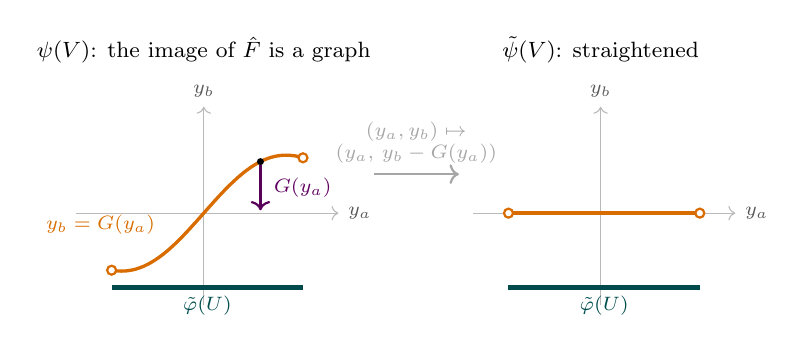
\begin{tikzpicture}[scale=0.9]
\draw[->, gray!55] (-1.80,0) -- (1.90,0) node[right, font=\scriptsize, text=gray!70!black] {$y_a$};
\draw[->, gray!55] (0.00,-1.3) -- (0.00,1.5) node[above, font=\scriptsize, text=gray!70!black] {$y_b$};
\node[font=\footnotesize] at (0.00,2.3) {$\psi(V)$: the image of $\hat F$ is a graph};
\draw[->, gray!55] (3.80,0) -- (7.50,0) node[right, font=\scriptsize, text=gray!70!black] {$y_a$};
\draw[->, gray!55] (5.60,-1.3) -- (5.60,1.5) node[above, font=\scriptsize, text=gray!70!black] {$y_b$};
\node[font=\footnotesize] at (5.60,2.3) {$\tilde\psi(V)$: straightened};
\draw[orange!85!black, very thick] (-1.300,-0.805) -- (-1.277,-0.809) -- (-1.255,-0.812) -- (-1.232,-0.815) -- (-1.209,-0.816) -- (-1.187,-0.817) -- (-1.164,-0.818) -- (-1.141,-0.817) -- (-1.118,-0.817) -- (-1.096,-0.815) -- (-1.073,-0.812) -- (-1.050,-0.809) -- (-1.028,-0.805) -- (-1.005,-0.801) -- (-0.982,-0.796) -- (-0.960,-0.790) -- (-0.937,-0.783) -- (-0.914,-0.775) -- (-0.892,-0.767) -- (-0.869,-0.758) -- (-0.846,-0.749) -- (-0.824,-0.738) -- (-0.801,-0.727) -- (-0.778,-0.716) -- (-0.755,-0.703) -- (-0.733,-0.690) -- (-0.710,-0.676) -- (-0.687,-0.662) -- (-0.665,-0.647) -- (-0.642,-0.631) -- (-0.619,-0.615) -- (-0.597,-0.598) -- (-0.574,-0.581) -- (-0.551,-0.562) -- (-0.529,-0.544) -- (-0.506,-0.525) -- (-0.483,-0.505) -- (-0.461,-0.485) -- (-0.438,-0.464) -- (-0.415,-0.443) -- (-0.392,-0.421) -- (-0.370,-0.399) -- (-0.347,-0.377) -- (-0.324,-0.354) -- (-0.302,-0.331) -- (-0.279,-0.307) -- (-0.256,-0.283) -- (-0.234,-0.259) -- (-0.211,-0.235) -- (-0.188,-0.210) -- (-0.166,-0.185) -- (-0.143,-0.160) -- (-0.120,-0.135) -- (-0.097,-0.110) -- (-0.075,-0.084) -- (-0.052,-0.059) -- (-0.029,-0.033) -- (-0.007,-0.008) -- (0.016,0.018) -- (0.039,0.044) -- (0.061,0.069) -- (0.084,0.095) -- (0.107,0.120) -- (0.129,0.145) -- (0.152,0.171) -- (0.175,0.196) -- (0.197,0.220) -- (0.220,0.245) -- (0.243,0.269) -- (0.266,0.293) -- (0.288,0.317) -- (0.311,0.340) -- (0.334,0.363) -- (0.356,0.386) -- (0.379,0.408) -- (0.402,0.430) -- (0.424,0.451) -- (0.447,0.472) -- (0.470,0.493) -- (0.492,0.513) -- (0.515,0.532) -- (0.538,0.551) -- (0.561,0.570) -- (0.583,0.588) -- (0.606,0.605) -- (0.629,0.622) -- (0.651,0.638) -- (0.674,0.653) -- (0.697,0.668) -- (0.719,0.682) -- (0.742,0.696) -- (0.765,0.708) -- (0.787,0.720) -- (0.810,0.732) -- (0.833,0.743) -- (0.855,0.753) -- (0.878,0.762) -- (0.901,0.771) -- (0.924,0.778) -- (0.946,0.786) -- (0.969,0.792) -- (0.992,0.798) -- (1.014,0.803) -- (1.037,0.807) -- (1.060,0.811) -- (1.082,0.813) -- (1.105,0.816) -- (1.128,0.817) -- (1.150,0.818) -- (1.173,0.818) -- (1.196,0.817) -- (1.218,0.816) -- (1.241,0.814) -- (1.264,0.811) -- (1.287,0.808) -- (1.309,0.804) -- (1.332,0.799) -- (1.355,0.794) -- (1.377,0.788) -- (1.400,0.781);
\draw[orange!85!black, very thick] (4.30,0) -- (7.00,0);
\draw[orange!85!black, fill=white, thick] (-1.300,-0.805) circle (1.8pt);
\draw[orange!85!black, fill=white, thick] (1.400,0.781) circle (1.8pt);
\draw[orange!85!black, fill=white, thick] (4.300,-0.000) circle (1.8pt);
\draw[orange!85!black, fill=white, thick] (7.000,0.000) circle (1.8pt);
\draw[teal!60!black, line width=2pt] (-1.30,-1.05) -- (1.40,-1.05); \node[teal!60!black, font=\scriptsize] at (0.05,-1.3) {$\tilde\varphi(U)$};
\draw[teal!60!black, line width=2pt] (4.30,-1.05) -- (7.00,-1.05); \node[teal!60!black, font=\scriptsize] at (5.65,-1.3) {$\tilde\varphi(U)$};
\draw[->, thick, violet!70!black] (0.800,0.677) -- (0.800,0.04); \fill (0.800,0.727) circle (1.4pt); \node[violet!75!black, font=\scriptsize, anchor=west] at (0.850,0.363) {$G(y_a)$};
\node[orange!85!black, font=\scriptsize, anchor=south east] at (-0.55,-0.44) {$y_b = G(y_a)$};
\draw[->, thick, gray!70] (2.4,0.55) -- node[above, font=\scriptsize, align=center] {$(y_a, y_b) \mapsto$\\ $(y_a,\, y_b - G(y_a))$} (3.6,0.55);
\end{tikzpicture}
\end{center}

Step~6 in a picture ($m = n - m = 1$). Before: the image of $\hat F$ is the graph $y_b = G(y_a)$ over $\tilde\varphi(U)$. After: each point is moved straight down by $G(y_a)$, and the graph becomes a piece of the $y_a$-axis --- an open interval, over the same $\tilde\varphi(U)$.

\textbf{Transcription note.} Page~38 of the handwritten notes begins the proof with ``start with any coordinates with $\varphi(U) \subset V$''; the condition is $F(U) \subseteq V$. In the lecture the shifted coordinates were first spoken as $G^{i-m}(y^1, \ldots, y^n)$; the arguments are the first $m$ coordinates, $y^1, \ldots, y^m$, as on page~38.

\begin{center}
\begin{tikzcd}[column sep=8em, row sep=3em]
U \arrow[r, "F"] \arrow[d, "\varphi"'] & V \arrow[d, "\psi"] \\
\varphi(U) \arrow[r, "{\tilde F :\ r \,\mapsto\, (r, \vec 0)}"'] & \psi(V)
\end{tikzcd}
\end{center}

The immersion normal form, as on the board: the mirror image of the submersion normal form (Theorem~\ref{thm:submersion-normal-form}). There $\tilde F$ forgot the last $m - n$ coordinates; here it appends $n - m$ zeros.

\textit{Status.} Stated in Lecture~13 --- ``a little bit technical \ldots\ better do it fresh at the beginning of the class'' --- and proved at the start of Lecture~14, above. It is the counterpart of Theorem~\ref{thm:submersion-normal-form}: there $F$ was locally a projection, here it is locally an inclusion.

What the image of an immersion looks like --- locally a submanifold, globally not necessarily --- is taken up next, in \ref{sub:immersion-images}.

\subsection{Images of Immersions}\label{sub:immersion-images}

\textit{Lecture 13, continuing \ref{sub:immersions}. What the image of an immersion looks like. These results use submanifolds (\ref{sub:submanifolds}).}

\begin{corbox}[The Local Image of an Immersion]\thmlabel{cor:immersion-local-image}
In the charts of Theorem~\ref{thm:immersion-normal-form}, $F|_U$ is injective and $F(U)$ is a submanifold of $N$ of codimension $n - m$.
\end{corbox}

\begin{proof}
\textit{(Lecture~13 gave the idea --- the image of $\tilde F$ is an open set times zeros, ``and so since what happens below happens upstairs too'', $F(U)$ is a submanifold --- adding ``I'm feeling a little bit uneasy, because I want to say after restriction, possibly after restricting $U$.'' Completed here: shrinking $V$ instead of $U$ settles it.)} $\tilde F$ is injective, so $F|_U$ is. Let
\[
V' = \big\{\, q \in V : \big(y^1(q), \ldots, y^m(q)\big) \in \varphi(U) \,\big\},
\]
open in $N$ because $\varphi(U)$ is open, and containing $F(U)$ because $\psi(F(u)) = (\varphi(u), \vec 0)$. We claim $F(U) = \{ q \in V' : y^{m+1}(q) = \cdots = y^n(q) = 0 \}$. The inclusion $\subseteq$ is clear. Conversely, if $q \in V'$ has $\psi(q) = (r, \vec 0)$ with $r \in \varphi(U)$, then $\psi(q) = \tilde F(r) = \psi\big(F(\varphi^{-1}(r))\big)$, so $q = F(\varphi^{-1}(r))$ because $\psi$ is injective. So $(V', \psi|_{V'})$ is an adapted chart (Definition~\ref{def:submanifold}) at every point of $F(U)$, and $F(U)$ is a submanifold of codimension $n - m$. No restriction of $U$ was needed: the worry was that $\psi(V) \cap (\mathbb{R}^m \times \{\vec 0\})$ might contain points not of the form $\tilde F(r)$ with $r \in \varphi(U)$, and passing to $V'$ removes exactly those.
\end{proof}

``But the really interesting thing about these immersions is that globally it doesn't have to be the case'': the whole image of an immersion need not be a submanifold. There are two ways for this to fail.

\begin{exbox}[An Immersion That Crosses Itself]\exlabel{ex:nodal-cubic}
$\gamma : \mathbb{R} \to \mathbb{R}^2$, $\gamma(t) = (t^2 - 1, \ t^3 - t)$, is an immersion, but it is not injective, and its image is not a submanifold of $\mathbb{R}^2$: near the origin the image looks like an X.
\end{exbox}

\begin{proof}
\textit{(Lecture~13 drew a curve crossing itself and gave the argument below; the specific curve is filled in.)} $\gamma'(t) = (2t, 3t^2 - 1)$ never vanishes --- the first component vanishes only at $t = 0$, where the second is $-1$ --- so $\gamma$ is an immersion. And $\gamma(1) = \gamma(-1) = (0, 0)$, so $\gamma$ is not injective. Near the origin the image consists of two arcs crossing transversally, one through $\gamma(-1)$ and one through $\gamma(1)$, with tangent directions $\gamma'(\mp 1) = (\mp 2, 2)$. ``What is the proof? If you remove the point of intersection from an X, you get four connected components. If you remove a point from an interval, you get two.'' This is the lecture's level of rigour: made precise, it compares small connected neighbourhoods of the crossing point in the image with those of a point of a $1$-manifold.
\end{proof}

\begin{center}
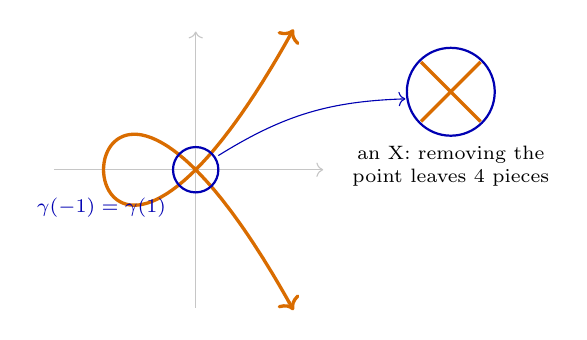
\begin{tikzpicture}[scale=0.9]
\draw[->, gray!45] (-2.0,0) -- (1.8,0); \draw[->, gray!45] (0,-1.95) -- (0,1.95);
\draw[orange!85!black, very thick] (1.321,-1.876) -- (1.286,-1.814) -- (1.252,-1.754) -- (1.217,-1.694) -- (1.183,-1.635) -- (1.149,-1.577) -- (1.115,-1.520) -- (1.082,-1.464) -- (1.048,-1.409) -- (1.015,-1.355) -- (0.982,-1.302) -- (0.950,-1.249) -- (0.917,-1.198) -- (0.885,-1.148) -- (0.853,-1.098) -- (0.822,-1.050) -- (0.790,-1.002) -- (0.759,-0.955) -- (0.728,-0.909) -- (0.697,-0.864) -- (0.667,-0.820) -- (0.637,-0.777) -- (0.607,-0.735) -- (0.577,-0.693) -- (0.547,-0.652) -- (0.518,-0.612) -- (0.489,-0.573) -- (0.460,-0.535) -- (0.431,-0.498) -- (0.403,-0.461) -- (0.375,-0.425) -- (0.347,-0.390) -- (0.319,-0.356) -- (0.292,-0.323) -- (0.265,-0.290) -- (0.238,-0.258) -- (0.211,-0.227) -- (0.184,-0.197) -- (0.158,-0.167) -- (0.132,-0.139) -- (0.106,-0.111) -- (0.081,-0.083) -- (0.055,-0.057) -- (0.030,-0.031) -- (0.005,-0.005) -- (-0.019,0.019) -- (-0.044,0.043) -- (-0.068,0.066) -- (-0.092,0.088) -- (-0.115,0.110) -- (-0.139,0.131) -- (-0.162,0.152) -- (-0.185,0.171) -- (-0.208,0.190) -- (-0.230,0.209) -- (-0.253,0.227) -- (-0.275,0.244) -- (-0.296,0.260) -- (-0.318,0.276) -- (-0.339,0.292) -- (-0.361,0.306) -- (-0.381,0.321) -- (-0.402,0.334) -- (-0.422,0.347) -- (-0.443,0.359) -- (-0.463,0.371) -- (-0.482,0.382) -- (-0.502,0.393) -- (-0.521,0.403) -- (-0.540,0.413) -- (-0.559,0.422) -- (-0.577,0.430) -- (-0.596,0.438) -- (-0.614,0.446) -- (-0.631,0.453) -- (-0.649,0.459) -- (-0.666,0.465) -- (-0.684,0.471) -- (-0.700,0.476) -- (-0.717,0.480) -- (-0.733,0.484) -- (-0.750,0.488) -- (-0.766,0.491) -- (-0.781,0.494) -- (-0.797,0.496) -- (-0.812,0.498) -- (-0.827,0.499) -- (-0.842,0.500) -- (-0.856,0.500) -- (-0.871,0.500) -- (-0.885,0.500) -- (-0.899,0.499) -- (-0.912,0.498) -- (-0.926,0.497) -- (-0.939,0.495) -- (-0.952,0.493) -- (-0.964,0.490) -- (-0.977,0.487) -- (-0.989,0.484) -- (-1.001,0.480) -- (-1.013,0.476) -- (-1.024,0.472) -- (-1.035,0.467) -- (-1.046,0.462) -- (-1.057,0.457) -- (-1.068,0.451) -- (-1.078,0.445) -- (-1.088,0.439) -- (-1.098,0.433) -- (-1.108,0.426) -- (-1.117,0.419) -- (-1.126,0.412) -- (-1.135,0.404) -- (-1.144,0.397) -- (-1.152,0.389) -- (-1.160,0.380) -- (-1.168,0.372) -- (-1.176,0.363) -- (-1.184,0.354) -- (-1.191,0.345) -- (-1.198,0.336) -- (-1.205,0.326) -- (-1.211,0.316) -- (-1.218,0.306) -- (-1.224,0.296) -- (-1.230,0.286) -- (-1.235,0.276) -- (-1.241,0.265) -- (-1.246,0.254) -- (-1.251,0.244) -- (-1.255,0.233) -- (-1.260,0.221) -- (-1.264,0.210) -- (-1.268,0.199) -- (-1.272,0.187) -- (-1.275,0.176) -- (-1.279,0.164) -- (-1.282,0.152) -- (-1.284,0.140) -- (-1.287,0.128) -- (-1.289,0.116) -- (-1.292,0.104) -- (-1.293,0.092) -- (-1.295,0.080) -- (-1.296,0.068) -- (-1.298,0.055) -- (-1.299,0.043) -- (-1.299,0.031) -- (-1.300,0.019) -- (-1.300,0.006) -- (-1.300,-0.006) -- (-1.300,-0.019) -- (-1.299,-0.031) -- (-1.299,-0.043) -- (-1.298,-0.055) -- (-1.296,-0.068) -- (-1.295,-0.080) -- (-1.293,-0.092) -- (-1.292,-0.104) -- (-1.289,-0.116) -- (-1.287,-0.128) -- (-1.284,-0.140) -- (-1.282,-0.152) -- (-1.279,-0.164) -- (-1.275,-0.176) -- (-1.272,-0.187) -- (-1.268,-0.199) -- (-1.264,-0.210) -- (-1.260,-0.221) -- (-1.255,-0.233) -- (-1.251,-0.244) -- (-1.246,-0.254) -- (-1.241,-0.265) -- (-1.235,-0.276) -- (-1.230,-0.286) -- (-1.224,-0.296) -- (-1.218,-0.306) -- (-1.211,-0.316) -- (-1.205,-0.326) -- (-1.198,-0.336) -- (-1.191,-0.345) -- (-1.184,-0.354) -- (-1.176,-0.363) -- (-1.168,-0.372) -- (-1.160,-0.380) -- (-1.152,-0.389) -- (-1.144,-0.397) -- (-1.135,-0.404) -- (-1.126,-0.412) -- (-1.117,-0.419) -- (-1.108,-0.426) -- (-1.098,-0.433) -- (-1.088,-0.439) -- (-1.078,-0.445) -- (-1.068,-0.451) -- (-1.057,-0.457) -- (-1.046,-0.462) -- (-1.035,-0.467) -- (-1.024,-0.472) -- (-1.013,-0.476) -- (-1.001,-0.480) -- (-0.989,-0.484) -- (-0.977,-0.487) -- (-0.964,-0.490) -- (-0.952,-0.493) -- (-0.939,-0.495) -- (-0.926,-0.497) -- (-0.912,-0.498) -- (-0.899,-0.499) -- (-0.885,-0.500) -- (-0.871,-0.500) -- (-0.856,-0.500) -- (-0.842,-0.500) -- (-0.827,-0.499) -- (-0.812,-0.498) -- (-0.797,-0.496) -- (-0.781,-0.494) -- (-0.766,-0.491) -- (-0.750,-0.488) -- (-0.733,-0.484) -- (-0.717,-0.480) -- (-0.700,-0.476) -- (-0.684,-0.471) -- (-0.666,-0.465) -- (-0.649,-0.459) -- (-0.631,-0.453) -- (-0.614,-0.446) -- (-0.596,-0.438) -- (-0.577,-0.430) -- (-0.559,-0.422) -- (-0.540,-0.413) -- (-0.521,-0.403) -- (-0.502,-0.393) -- (-0.482,-0.382) -- (-0.463,-0.371) -- (-0.443,-0.359) -- (-0.422,-0.347) -- (-0.402,-0.334) -- (-0.381,-0.321) -- (-0.361,-0.306) -- (-0.339,-0.292) -- (-0.318,-0.276) -- (-0.296,-0.260) -- (-0.275,-0.244) -- (-0.253,-0.227) -- (-0.230,-0.209) -- (-0.208,-0.190) -- (-0.185,-0.171) -- (-0.162,-0.152) -- (-0.139,-0.131) -- (-0.115,-0.110) -- (-0.092,-0.088) -- (-0.068,-0.066) -- (-0.044,-0.043) -- (-0.019,-0.019) -- (0.005,0.005) -- (0.030,0.031) -- (0.055,0.057) -- (0.081,0.083) -- (0.106,0.111) -- (0.132,0.139) -- (0.158,0.167) -- (0.184,0.197) -- (0.211,0.227) -- (0.238,0.258) -- (0.265,0.290) -- (0.292,0.323) -- (0.319,0.356) -- (0.347,0.390) -- (0.375,0.425) -- (0.403,0.461) -- (0.431,0.498) -- (0.460,0.535) -- (0.489,0.573) -- (0.518,0.612) -- (0.547,0.652) -- (0.577,0.693) -- (0.607,0.735) -- (0.637,0.777) -- (0.667,0.820) -- (0.697,0.864) -- (0.728,0.909) -- (0.759,0.955) -- (0.790,1.002) -- (0.822,1.050) -- (0.853,1.098) -- (0.885,1.148) -- (0.917,1.198) -- (0.950,1.249) -- (0.982,1.302) -- (1.015,1.355) -- (1.048,1.409) -- (1.082,1.464) -- (1.115,1.520) -- (1.149,1.577) -- (1.183,1.635) -- (1.217,1.694) -- (1.252,1.754) -- (1.286,1.814) -- (1.321,1.876);
\draw[blue!70!black, thick] (0,0) circle (0.32);
\node[blue!70!black, font=\scriptsize, anchor=north east] at (-0.28,-0.26) {$\gamma(-1) = \gamma(1)$};
\draw[blue!70!black, thick] (3.60,1.10) circle (0.62);
\draw[orange!85!black, very thick] (3.18,0.68) -- (4.02,1.52);
\draw[orange!85!black, very thick] (3.18,1.52) -- (4.02,0.68);
\draw[->, blue!70!black] (0.32,0.2) to[bend left=15] (2.96,1.00);
\node[font=\scriptsize, align=center] at (3.60,0.05) {an X: removing the\\ point leaves 4 pieces};
\draw[->, orange!85!black, very thick] (1.316,-1.868) -- (1.381,-1.981);
\draw[->, orange!85!black, very thick] (1.316,1.868) -- (1.381,1.981);
\end{tikzpicture}
\end{center}

The nodal cubic. The parameter values $t = -1$ and $t = 1$ both land on the origin, where the two branches cross; the arrows show the curve continuing, its domain being all of $\mathbb{R}$. A small disc around the crossing meets the image in an X, which is not a piece of a line.

\begin{exbox}[An Injective Immersion That Is Not a Homeomorphism onto Its Image]\exlabel{ex:hook}
Let $\gamma : (a, b) \to \mathbb{R}^2$ be an injective immersion that passes through a point $P = \gamma(t_0)$ and whose other end returns to $P$: $\gamma(t) \to P$ as $t \to b$. Then $\gamma$ is not a homeomorphism onto its image, and near $P$ the image looks like a T.
\end{exbox}

\begin{proof}
\textit{(Lecture~13: ``it's like you're making a hook with a piece of wire \ldots\ but the wire is open, it doesn't have an end''; the discontinuity argument is filled in.)} Choose $t_k \to b$. Then $\gamma(t_k) \to P = \gamma(t_0)$ in the image, but $t_k \to b \ne t_0$, so $\gamma^{-1}(\gamma(t_k)) = t_k$ does not converge to $\gamma^{-1}(P) = t_0$. So $\gamma^{-1} : \gamma\big((a,b)\big) \to (a, b)$ is not continuous at $P$. The image near $P$ consists of the strand through $P$ together with the end arriving at it: ``this point now doesn't look like an X, but it looks like a T''; removing it leaves three pieces, not two.
\end{proof}

\begin{center}
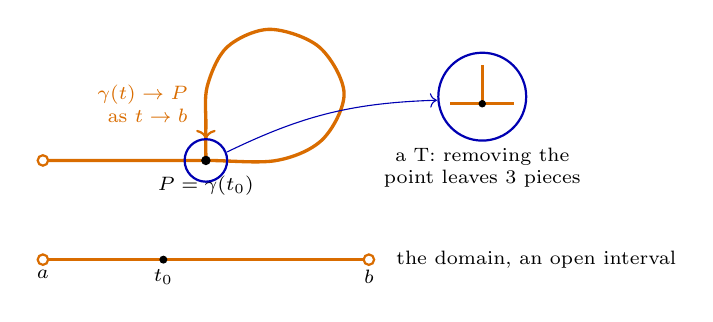
\begin{tikzpicture}[scale=0.9]
\draw[orange!85!black, very thick] plot[smooth, tension=0.55] coordinates {(-2.3,0) (-1.2,0) (0,0) (1.0,0.0) (1.65,0.3) (1.95,0.95) (1.6,1.6) (0.9,1.85) (0.3,1.6) (0.02,1.05) (0,0.5) (0,0)};
\draw[orange!85!black, fill=white, thick] (-2.3,0) circle (2.1pt);
\fill (0,0) circle (1.9pt); \node[font=\scriptsize, anchor=north] at (0,-0.08) {$P = \gamma(t_0)$};
\draw[->, orange!85!black, thick] (0,0.62) -- (0,0.3);
\node[orange!85!black, font=\scriptsize, anchor=east, align=right] at (-0.12,0.8) {$\gamma(t) \to P$\\ as $t \to b$};
\draw[blue!70!black, thick] (0,0) circle (0.3);
\draw[blue!70!black, thick] (3.90,0.90) circle (0.62);
\draw[orange!85!black, very thick] (3.45,0.80) -- (4.35,0.80); \draw[orange!85!black, very thick] (3.90,0.80) -- (3.90,1.35);
\fill (3.90,0.80) circle (1.5pt);
\draw[->, blue!70!black] (0.3,0.12) to[bend left=12] (3.26,0.85);
\node[font=\scriptsize, align=center] at (3.90,-0.10) {a T: removing the\\ point leaves 3 pieces};
\draw[orange!85!black, very thick] (-2.3,-1.4) -- (2.3,-1.4); \draw[orange!85!black, fill=white, thick] (-2.3,-1.4) circle (2.1pt) node[below, font=\scriptsize, text=black] {$a$}; \draw[orange!85!black, fill=white, thick] (2.3,-1.4) circle (2.1pt) node[below, font=\scriptsize, text=black] {$b$};
\fill (-0.6,-1.4) circle (1.6pt) node[below, font=\scriptsize] {$t_0$};
\node[font=\scriptsize, anchor=west] at (2.55,-1.4) {the domain, an open interval};
\end{tikzpicture}
\end{center}

The hook. The domain is an open interval, so neither end is attained: the left end of the image is missing (hollow), and the right end only approaches $P$. But $P$ is in the image, reached at $t_0$ by the strand passing through it --- so points of the image near $P$ come from parameters near $t_0$ \emph{and} from parameters near $b$, which is exactly the failure of continuity of $\gamma^{-1}$. Lee's figure-eight (Example~4.19) is an explicit instance with both ends returning, $\beta(t) = (\sin 2t, \sin t)$ on $(-\pi, \pi)$, where the image near the origin is an X although $\beta$ is injective.

\begin{rembox}[Embeddings --- Next Time]\label{rem:embeddings-next-time}
To make the image of an immersion a submanifold, ``you have to add a topological condition'': an \emph{embedding} is an immersion that is a homeomorphism onto its image, and its image is a submanifold. Both were done in Lecture~14, together with the proof of the normal form above: see \ref{sec:embeddings}.
\end{rembox}

% ============================================================
% Lecture 14 (Fri Oct 2, 2026)
% ============================================================

\section{Embeddings}\label{sec:embeddings}

\roadmark{Stage: maps}{Immersions that are homeomorphisms onto their images --- their images are submanifolds.}

\textit{References: Lee Ch.~4 and Ch.~5. Lecture 14.} The normal form makes every immersion locally an inclusion, but an immersion's image can still fail to be a submanifold (\ref{sub:immersion-images}). Embeddings are the immersions for which it cannot: the normal form is local in the domain, and the topological condition makes it local in the image too.

\subsection{Embeddings and Their Images}\label{sub:embeddings}

\begin{defbox}[Embedding]\deflabel{def:embedding}
A smooth map $F : M \to N$ is an \textbf{embedding} if it is an immersion and, as a map onto its image, $F : M \to F(M)$ is a homeomorphism, $F(M)$ carrying the subspace topology of $N$. Injectivity is part of being a homeomorphism; Uribe wrote ``(injective) immersion'' and called the word redundant.
\leeref{Ch.~4, \emph{Embeddings}}
\end{defbox}

\begin{center}
\begin{tikzcd}[column sep=4.2em, row sep=2.8em]
M \arrow[r, "\cong", "F"'] \arrow[dr, "F"'] & F(M) \arrow[d, hook] \\
& N
\end{tikzcd}
\end{center}

An embedding factors through its image as a homeomorphism followed by the inclusion --- ``you're taking the manifold $M$ and you're putting it inside $N$.'' The figure-eight of Lee's Example~4.19 (\ref{sub:immersion-images}) is an injective immersion for which the top arrow is not a homeomorphism.

The standard non-example is the \emph{irrational line on the torus}: for $\alpha$ irrational, $F : \mathbb{R} \to T^2 = \mathbb{R}^2/\mathbb{Z}^2$, $F(t) = [t, \alpha t]$. It is an injective immersion whose image is dense in $T^2$, and it is not an embedding (Proposition~\ref{prop:irrational-line} below, from Assignment~4, Problem~5; Lee, Example~4.20). In lecture its image was also said not to be a regular submanifold of $T^2$.

\textit{In lecture.} Given as ``a very important category: non-examples.'' ``You're wrapping a line, but the slope of the line is irrational, so it never closes \ldots\ like one of those spirographs.'' The normal form still applies: around any $p$ there are neighbourhoods $U$ and $V$ for which $F(U)$ is ``a very nice submanifold.'' But ``it's local in the domain'', while being a submanifold is a statement about the whole image. Points outside $U$ ``contribute segments like this, and they're going to be dense. No matter how you shrink this $V$, you won't be able to isolate only the yellow guy.''

\begin{center}
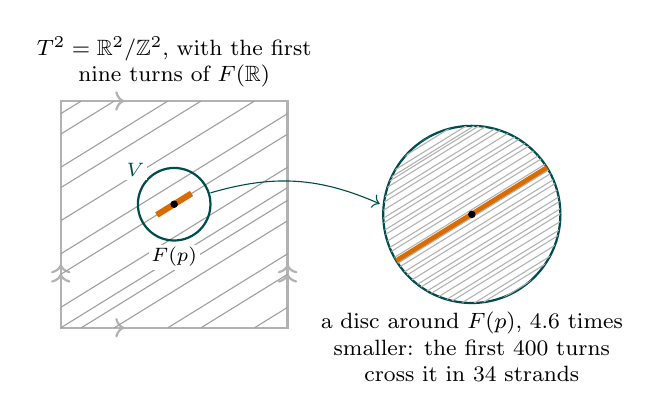
\begin{tikzpicture}[scale=0.9]
\draw[gray!60, thick] (0,0) rectangle (3.20,3.20);
\draw[->, gray!60, thick] (0.5,0) -- (0.9,0); \draw[->, gray!60, thick] (0.5,3.20) -- (0.9,3.20); \draw[->>, gray!60, thick] (0,0.5) -- (0,0.9); \draw[->>, gray!60, thick] (3.20,0.5) -- (3.20,0.9);
\draw[gray!75] (0.000,0.000) -- (3.200,1.978);
\draw[gray!75] (0.000,1.978) -- (1.978,3.200);
\draw[gray!75] (1.978,0.000) -- (3.200,0.755);
\draw[gray!75] (0.000,0.755) -- (3.200,2.733);
\draw[gray!75] (0.000,2.733) -- (0.755,3.200);
\draw[gray!75] (0.755,0.000) -- (3.200,1.511);
\draw[gray!75] (0.000,1.511) -- (2.733,3.200);
\draw[gray!75] (2.733,0.000) -- (3.200,0.289);
\draw[gray!75] (0.000,0.289) -- (3.200,2.266);
\draw[gray!75] (0.000,2.266) -- (1.511,3.200);
\draw[gray!75] (1.511,0.000) -- (3.200,1.044);
\draw[gray!75] (0.000,1.044) -- (3.200,3.022);
\draw[gray!75] (0.000,3.022) -- (0.289,3.200);
\draw[gray!75] (0.289,0.000) -- (3.200,1.799);
\draw[orange!85!black, line width=2.2pt] (1.355,1.593) -- (1.845,1.896);
\draw[teal!60!black, thick] (1.600,1.744) circle (0.512);
\fill (1.600,1.744) circle (1.5pt);
\node[font=\scriptsize, fill=white, inner sep=1pt, anchor=north] at (1.600,1.182) {$F(p)$};
\node[teal!60!black, font=\scriptsize, fill=white, inner sep=1pt] at (1.056,2.224) {$V$};
\node[font=\footnotesize, align=center] at (1.60,3.75) {$T^2 = \mathbb{R}^2/\mathbb{Z}^2$, with the first\\ nine turns of $F(\mathbb{R})$};
\draw[teal!60!black, thick] (5.80,1.60) circle (1.25);
\begin{scope}\clip (5.80,1.60) circle (1.25);
\draw[orange!85!black, line width=2pt] (4.439,0.759) -- (7.161,2.441);
\draw[gray!60] (3.889,1.649) -- (6.611,3.331);
\draw[gray!60] (4.779,0.209) -- (7.501,1.891);
\draw[gray!60] (4.229,1.099) -- (6.951,2.781);
\draw[gray!60] (4.569,0.549) -- (7.291,2.231);
\draw[gray!60] (4.019,1.439) -- (6.741,3.121);
\draw[gray!60] (4.909,-0.001) -- (7.631,1.681);
\draw[gray!60] (4.359,0.889) -- (7.081,2.571);
\draw[gray!60] (3.809,1.779) -- (6.531,3.461);
\draw[gray!60] (4.699,0.339) -- (7.421,2.021);
\draw[gray!60] (4.149,1.229) -- (6.871,2.911);
\draw[gray!60] (5.039,-0.212) -- (7.761,1.471);
\draw[gray!60] (4.489,0.679) -- (7.211,2.361);
\draw[gray!60] (3.938,1.569) -- (6.661,3.251);
\draw[gray!60] (4.829,0.128) -- (7.551,1.811);
\draw[gray!60] (4.278,1.019) -- (7.001,2.701);
\draw[gray!60] (4.618,0.468) -- (7.341,2.151);
\draw[gray!60] (4.068,1.359) -- (6.790,3.041);
\draw[gray!60] (4.958,-0.082) -- (7.680,1.601);
\draw[gray!60] (4.408,0.808) -- (7.130,2.491);
\draw[gray!60] (3.858,1.699) -- (6.580,3.381);
\draw[gray!60] (4.748,0.258) -- (7.470,1.941);
\draw[gray!60] (4.198,1.148) -- (6.920,2.831);
\draw[gray!60] (5.088,-0.292) -- (7.810,1.391);
\draw[gray!60] (4.538,0.598) -- (7.260,2.281);
\draw[gray!60] (3.988,1.488) -- (6.710,3.171);
\draw[gray!60] (4.878,0.048) -- (7.600,1.731);
\draw[gray!60] (4.328,0.938) -- (7.050,2.621);
\draw[gray!60] (3.778,1.828) -- (6.500,3.511);
\draw[gray!60] (4.668,0.388) -- (7.390,2.071);
\draw[gray!60] (4.118,1.278) -- (6.840,2.961);
\draw[gray!60] (5.008,-0.162) -- (7.730,1.520);
\draw[gray!60] (4.458,0.728) -- (7.180,2.411);
\draw[gray!60] (3.908,1.618) -- (6.630,3.301);
\end{scope}
\fill (5.80,1.60) circle (1.5pt);
\draw[->, teal!60!black] (2.112,1.904) to[bend left=20] (4.50,1.75);
\node[font=\footnotesize, align=center] at (5.80,-0.27) {a disc around $F(p)$, 4.6 times\\ smaller: the first 400 turns\\ cross it in 34 strands};
\end{tikzpicture}
\end{center}

The irrational line, drawn here with $\alpha = (\sqrt5 - 1)/2$. Left: nine turns of $F(\mathbb{R})$ in the square, whose opposite sides are identified; the orange piece is $F(U)$, and two other strands already cross the neighbourhood $V$. Right: a disc around $F(p)$ about $4.6$ times smaller, and the first 400 turns of the curve, which cross it in 34 strands. Shrinking further only takes more turns: every neighbourhood of $F(p)$ meets infinitely many strands.

\begin{thmbox}[The Image of an Embedding Is a Submanifold]\thmlabel{thm:embedding-image}
If $F : M \to N$ is an embedding, with $\dim M = m$ and $\dim N = n$, then $F(M)$ is a regular submanifold of $N$ of codimension $n - m$.
\leeref{Proposition 5.2}
\end{thmbox}

\begin{proof}
\textit{(Lecture~14. The final equality is completed with Corollary~\ref{cor:immersion-local-image}; see the remark after the proof.)} Let $q = F(p) \in F(M)$. We need a chart of $N$ at $q$ in which $F(M)$ is cut out by the vanishing of the last $n - m$ coordinates.

\emph{Start with the normal form.} Take the charts $(U, \varphi)$ at $p$ and $(V, \psi = (y^1, \ldots, y^n))$ at $q$ of Theorem~\ref{thm:immersion-normal-form}. By Corollary~\ref{cor:immersion-local-image}, after replacing $V$ by the smaller open set
\[
V' = \big\{\, x \in V : \big(y^1(x), \ldots, y^m(x)\big) \in \varphi(U) \,\big\},
\]
we have
\[
F(U) = \{\, x \in V' : y^{m+1}(x) = \cdots = y^n(x) = 0 \,\}. \tag{$*$}
\]
This describes $F(U)$, not $F(M) \cap V'$: ``other pieces of the image'' may still pass through $V'$, as in the irrational line.

\emph{The key step: the topological hypothesis.} ``Here's where we use the very strong condition that $F$ is a topological homeomorphism to its image.'' $U$ is open in $M$ and $F : M \to F(M)$ is a homeomorphism, so $F(U)$ is open in $F(M)$: there is an open $W \subseteq N$ with
\[
F(U) = W \cap F(M) .
\]

\emph{Shrink $V'$ to $V' \cap W$, and keep the same coordinates.} Since $F(U) \subseteq V' \cap W$,
\[
F(M) \cap (V' \cap W) = F(U) = \{\, x \in V' \cap W : y^{m+1}(x) = \cdots = y^n(x) = 0 \,\},
\]
the first equality because $F(M) \cap W = F(U) \subseteq V'$, the second by $(*)$ intersected with $W$. So $(V' \cap W, \psi)$ is an adapted chart at $q$ (Definition~\ref{def:submanifold}), and $F(M)$ is a submanifold of codimension $n - m$.
\end{proof}

\begin{center}
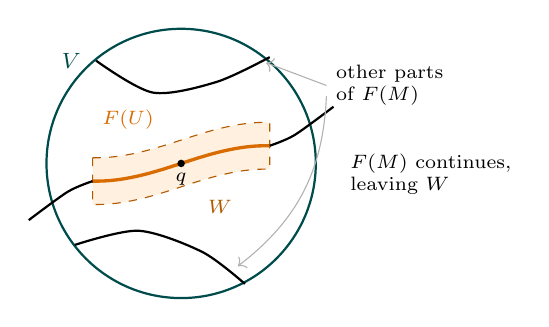
\begin{tikzpicture}[scale=0.9]
\draw[teal!60!black, thick] (0,0) circle (1.9); \node[teal!60!black, font=\footnotesize] at (-1.55,1.45) {$V$};
\fill[orange!12] (-1.250,0.080) -- (-1.208,0.080) -- (-1.165,0.080) -- (-1.123,0.082) -- (-1.081,0.083) -- (-1.038,0.086) -- (-0.996,0.089) -- (-0.953,0.094) -- (-0.911,0.098) -- (-0.869,0.104) -- (-0.826,0.110) -- (-0.784,0.117) -- (-0.742,0.125) -- (-0.699,0.133) -- (-0.657,0.142) -- (-0.614,0.151) -- (-0.572,0.161) -- (-0.530,0.171) -- (-0.487,0.182) -- (-0.445,0.193) -- (-0.403,0.205) -- (-0.360,0.217) -- (-0.318,0.230) -- (-0.275,0.242) -- (-0.233,0.255) -- (-0.191,0.269) -- (-0.148,0.282) -- (-0.106,0.296) -- (-0.064,0.309) -- (-0.021,0.323) -- (0.021,0.337) -- (0.064,0.351) -- (0.106,0.364) -- (0.148,0.378) -- (0.191,0.391) -- (0.233,0.405) -- (0.275,0.418) -- (0.318,0.430) -- (0.360,0.443) -- (0.403,0.455) -- (0.445,0.467) -- (0.487,0.478) -- (0.530,0.489) -- (0.572,0.499) -- (0.614,0.509) -- (0.657,0.518) -- (0.699,0.527) -- (0.742,0.535) -- (0.784,0.543) -- (0.826,0.550) -- (0.869,0.556) -- (0.911,0.562) -- (0.953,0.566) -- (0.996,0.571) -- (1.038,0.574) -- (1.081,0.577) -- (1.123,0.578) -- (1.165,0.580) -- (1.208,0.580) -- (1.250,0.580) -- (1.250,-0.080) -- (1.208,-0.080) -- (1.165,-0.080) -- (1.123,-0.082) -- (1.081,-0.083) -- (1.038,-0.086) -- (0.996,-0.089) -- (0.953,-0.094) -- (0.911,-0.098) -- (0.869,-0.104) -- (0.826,-0.110) -- (0.784,-0.117) -- (0.742,-0.125) -- (0.699,-0.133) -- (0.657,-0.142) -- (0.614,-0.151) -- (0.572,-0.161) -- (0.530,-0.171) -- (0.487,-0.182) -- (0.445,-0.193) -- (0.403,-0.205) -- (0.360,-0.217) -- (0.318,-0.230) -- (0.275,-0.242) -- (0.233,-0.255) -- (0.191,-0.269) -- (0.148,-0.282) -- (0.106,-0.296) -- (0.064,-0.309) -- (0.021,-0.323) -- (-0.021,-0.337) -- (-0.064,-0.351) -- (-0.106,-0.364) -- (-0.148,-0.378) -- (-0.191,-0.391) -- (-0.233,-0.405) -- (-0.275,-0.418) -- (-0.318,-0.430) -- (-0.360,-0.443) -- (-0.403,-0.455) -- (-0.445,-0.467) -- (-0.487,-0.478) -- (-0.530,-0.489) -- (-0.572,-0.499) -- (-0.614,-0.509) -- (-0.657,-0.518) -- (-0.699,-0.527) -- (-0.742,-0.535) -- (-0.784,-0.543) -- (-0.826,-0.550) -- (-0.869,-0.556) -- (-0.911,-0.562) -- (-0.953,-0.566) -- (-0.996,-0.571) -- (-1.038,-0.574) -- (-1.081,-0.577) -- (-1.123,-0.578) -- (-1.165,-0.580) -- (-1.208,-0.580) -- (-1.250,-0.580) -- cycle; \draw[orange!70!black, dashed] (-1.250,0.080) -- (-1.208,0.080) -- (-1.165,0.080) -- (-1.123,0.082) -- (-1.081,0.083) -- (-1.038,0.086) -- (-0.996,0.089) -- (-0.953,0.094) -- (-0.911,0.098) -- (-0.869,0.104) -- (-0.826,0.110) -- (-0.784,0.117) -- (-0.742,0.125) -- (-0.699,0.133) -- (-0.657,0.142) -- (-0.614,0.151) -- (-0.572,0.161) -- (-0.530,0.171) -- (-0.487,0.182) -- (-0.445,0.193) -- (-0.403,0.205) -- (-0.360,0.217) -- (-0.318,0.230) -- (-0.275,0.242) -- (-0.233,0.255) -- (-0.191,0.269) -- (-0.148,0.282) -- (-0.106,0.296) -- (-0.064,0.309) -- (-0.021,0.323) -- (0.021,0.337) -- (0.064,0.351) -- (0.106,0.364) -- (0.148,0.378) -- (0.191,0.391) -- (0.233,0.405) -- (0.275,0.418) -- (0.318,0.430) -- (0.360,0.443) -- (0.403,0.455) -- (0.445,0.467) -- (0.487,0.478) -- (0.530,0.489) -- (0.572,0.499) -- (0.614,0.509) -- (0.657,0.518) -- (0.699,0.527) -- (0.742,0.535) -- (0.784,0.543) -- (0.826,0.550) -- (0.869,0.556) -- (0.911,0.562) -- (0.953,0.566) -- (0.996,0.571) -- (1.038,0.574) -- (1.081,0.577) -- (1.123,0.578) -- (1.165,0.580) -- (1.208,0.580) -- (1.250,0.580) -- (1.250,-0.080) -- (1.208,-0.080) -- (1.165,-0.080) -- (1.123,-0.082) -- (1.081,-0.083) -- (1.038,-0.086) -- (0.996,-0.089) -- (0.953,-0.094) -- (0.911,-0.098) -- (0.869,-0.104) -- (0.826,-0.110) -- (0.784,-0.117) -- (0.742,-0.125) -- (0.699,-0.133) -- (0.657,-0.142) -- (0.614,-0.151) -- (0.572,-0.161) -- (0.530,-0.171) -- (0.487,-0.182) -- (0.445,-0.193) -- (0.403,-0.205) -- (0.360,-0.217) -- (0.318,-0.230) -- (0.275,-0.242) -- (0.233,-0.255) -- (0.191,-0.269) -- (0.148,-0.282) -- (0.106,-0.296) -- (0.064,-0.309) -- (0.021,-0.323) -- (-0.021,-0.337) -- (-0.064,-0.351) -- (-0.106,-0.364) -- (-0.148,-0.378) -- (-0.191,-0.391) -- (-0.233,-0.405) -- (-0.275,-0.418) -- (-0.318,-0.430) -- (-0.360,-0.443) -- (-0.403,-0.455) -- (-0.445,-0.467) -- (-0.487,-0.478) -- (-0.530,-0.489) -- (-0.572,-0.499) -- (-0.614,-0.509) -- (-0.657,-0.518) -- (-0.699,-0.527) -- (-0.742,-0.535) -- (-0.784,-0.543) -- (-0.826,-0.550) -- (-0.869,-0.556) -- (-0.911,-0.562) -- (-0.953,-0.566) -- (-0.996,-0.571) -- (-1.038,-0.574) -- (-1.081,-0.577) -- (-1.123,-0.578) -- (-1.165,-0.580) -- (-1.208,-0.580) -- (-1.250,-0.580) -- cycle;
\draw[orange!85!black, very thick] (-1.250,-0.250) -- (-1.208,-0.250) -- (-1.165,-0.250) -- (-1.123,-0.248) -- (-1.081,-0.247) -- (-1.038,-0.244) -- (-0.996,-0.241) -- (-0.953,-0.236) -- (-0.911,-0.232) -- (-0.869,-0.226) -- (-0.826,-0.220) -- (-0.784,-0.213) -- (-0.742,-0.205) -- (-0.699,-0.197) -- (-0.657,-0.188) -- (-0.614,-0.179) -- (-0.572,-0.169) -- (-0.530,-0.159) -- (-0.487,-0.148) -- (-0.445,-0.137) -- (-0.403,-0.125) -- (-0.360,-0.113) -- (-0.318,-0.100) -- (-0.275,-0.088) -- (-0.233,-0.075) -- (-0.191,-0.061) -- (-0.148,-0.048) -- (-0.106,-0.034) -- (-0.064,-0.021) -- (-0.021,-0.007) -- (0.021,0.007) -- (0.064,0.021) -- (0.106,0.034) -- (0.148,0.048) -- (0.191,0.061) -- (0.233,0.075) -- (0.275,0.088) -- (0.318,0.100) -- (0.360,0.113) -- (0.403,0.125) -- (0.445,0.137) -- (0.487,0.148) -- (0.530,0.159) -- (0.572,0.169) -- (0.614,0.179) -- (0.657,0.188) -- (0.699,0.197) -- (0.742,0.205) -- (0.784,0.213) -- (0.826,0.220) -- (0.869,0.226) -- (0.911,0.232) -- (0.953,0.236) -- (0.996,0.241) -- (1.038,0.244) -- (1.081,0.247) -- (1.123,0.248) -- (1.165,0.250) -- (1.208,0.250) -- (1.250,0.250);
\draw[thick] plot[smooth] coordinates {(-1.25,-0.250) (-1.6,-0.400) (-2.15,-0.800)};
\draw[thick] plot[smooth] coordinates {(1.25,0.250) (1.6,0.400) (2.15,0.800)};
\fill (0,0) circle (1.5pt) node[below, font=\scriptsize] {$q$};
\node[orange!85!black, font=\scriptsize, fill=white, inner sep=1pt] at (-0.75,0.62) {$F(U)$};
\node[orange!70!black, font=\scriptsize] at (0.55,-0.62) {$W$};
\draw[thick] plot[smooth] coordinates {(-1.2,1.45) (-0.4,1.0) (0.5,1.15) (1.25,1.5)};
\draw[thick] plot[smooth] coordinates {(-1.5,-1.15) (-0.6,-0.95) (0.3,-1.25) (0.9,-1.7)};
\node[font=\scriptsize, anchor=west, align=left] at (2.05,1.1) {other parts\\ of $F(M)$};
\node[font=\scriptsize, anchor=west, align=left] at (2.25,-0.15) {$F(M)$ continues,\\ leaving $W$};
\draw[->, gray!60] (2.05,1.1) -- (1.2,1.42); \draw[->, gray!60] (2.05,0.95) to[bend left=25] (0.8,-1.45);
\end{tikzpicture}
\end{center}

The key step. $V$ may contain other parts of $F(M)$ (black) besides $F(U)$ (orange). Because $F(U)$ is open in $F(M)$, it is $W \cap F(M)$ for an open $W$ (shaded), and $W$ cuts the other parts away; $F(M)$ continues beyond $F(U)$ only by leaving $W$. For the irrational line no such $W$ exists, which is exactly the failure of openness.

\textbf{Transcription note.} Page~39 of the handwritten notes writes the target as $F(M) \cap V = \{0 = y^{n-m+1} = \cdots = y^m\}$; the vanishing coordinates are the last $n - m$ of them, $y^{m+1}, \ldots, y^n$, as the lecture said.

\begin{rembox}[Where Is Injectivity Used?]\label{rem:where-injectivity-used}
In lecture the last equality caused trouble, and a discussion. Uribe first located the use of injectivity there; a student pointed out that $(*)$ concerns only $F(U)$, and that the proof seems to need only that $F$ be an immersion which is open onto its image. Another student added covering-type examples: maps that are not injective but whose images are manifolds, such as $\mathbb{R} \to S^1$, $t \mapsto (\cos t, \sin t)$, or the two-to-one map $S^2 \to \mathbb{RP}^2$. Uribe agreed --- ``I don't think we're using injectivity'' --- and promised ``a definite conclusion by email.''

\emph{The conclusion, from Uribe's follow-up email.} The students were right: ``a proof that we did today does show that for an immersion that is open as a map onto its image (so for all $U$ open in $M$, $F(U)$ is open in $F(M)$), $F(M)$ is a submanifold. The map $F$ does not have to be injective.'' The proof uses exactly two things: the normal form (the immersion hypothesis), and that $F(U)$ is open in $F(M)$ for the $U$ of the normal form; with the completion via Corollary~\ref{cor:immersion-local-image} nothing else enters. Injectivity belongs to the \emph{idea} of an embedding --- ``the idea of an embedding is that it is an isomorphism between $M$ and its image'' (Corollary~\ref{cor:embedding-diffeo}) --- not to this proof. He added that ``being an immersion and an open map onto its image'' is ``an unusual class of maps.\@''
\end{rembox}

\begin{propbox}[Immersions That Are Open onto Their Images]\thmlabel{prop:immersion-open-image}
Let $F : M \to N$ be an immersion such that $F : M \to F(M)$ is an open map, $F(M)$ carrying the subspace topology. Then $F(M)$ is a regular submanifold of $N$ of codimension $n - m$.
\end{propbox}

\begin{proof}
\textit{(The conclusion of the class discussion, confirmed in Uribe's follow-up email.)} The proof of Theorem~\ref{thm:embedding-image}, word for word: openness of $F$ onto its image is all it used to produce $W$. For example, $t \mapsto (\cos t, \sin t)$ is an immersion of $\mathbb{R}$, open onto $S^1$ and far from injective --- every point of $S^1$ has infinitely many preimages --- and its image $S^1$ is a submanifold of $\mathbb{R}^2$. The figure-eight is not open onto its image, consistent with its image not being a submanifold.
\end{proof}

\begin{corbox}[An Embedding Is a Diffeomorphism onto Its Image]\thmlabel{cor:embedding-diffeo}
If $F : M \to N$ is an embedding, then $F : M \to F(M)$ is a diffeomorphism, $F(M)$ carrying its induced smooth structure as a submanifold.
\end{corbox}

\begin{proof}
\textit{(Stated in Lecture~14 --- ``an embedding restricts to a diffeomorphism between $M$ and the image''; filled in.)} $F : M \to F(M)$ is smooth by Lemma~\ref{lem:maps-into-submanifold}(2), and it is an immersion: its differential followed by the injective $\iota_*$ is the injective $F_*$. Both manifolds have dimension $m$, so it is a local diffeomorphism (Proposition~\ref{prop:dimension-constraints}(3)); being bijective, it is a diffeomorphism, its inverse being smooth near every point.
\end{proof}

\subsection{Proper Maps}\label{sub:proper-maps}

\textit{Lecture 14. When is an injective immersion an embedding? The homeomorphism condition is point-set topology, and a convenient sufficient condition is properness --- the same hypothesis as in Ehresmann's theorem (Theorem~\ref{thm:ehresmann}).}

\begin{defbox}[Proper Map]\deflabel{def:proper-map}
A continuous map $F : X \to Y$ is \textbf{proper} if $F^{-1}(K)$ is compact for every compact $K \subseteq Y$.
\leeref{App.~A, \emph{Proper Maps}}
\end{defbox}

\begin{propbox}[Proper Maps into Manifolds Are Closed]\thmlabel{prop:proper-closed}
Let $F : M \to N$ be a continuous proper map, $N$ a topological manifold. Then $F$ is closed: $F(C)$ is closed in $N$ for every closed $C \subseteq M$.
\leeref{Theorem A.57}
\end{propbox}

\begin{proof}
\textit{(Lecture~14 --- ``it's a very funny proof. You go back and forth literally.'' Uribe did not finish Claim~2 in lecture and sent the complete proof in his follow-up email; the completion of Claim~2 below is the notes' own.)} Let $C \subseteq M$ be closed.

\emph{Claim 1: $F(C) \cap K$ is closed for every compact $K \subseteq N$.} $F^{-1}(K)$ is compact, so $C \cap F^{-1}(K)$, a closed subset of it, is compact; its image $F\big(C \cap F^{-1}(K)\big)$ is compact, hence closed in the Hausdorff space $N$. And $F\big(C \cap F^{-1}(K)\big) = F(C) \cap K$: a point of the left side is $F(c)$ with $c \in C$ and $F(c) \in K$, and conversely.

\emph{Claim 2.} Let $q \in \overline{F(C)}$, and let $V$ be a neighbourhood of $q$ with compact closure (Proposition~\ref{prop:locally-compact}). Then $q \in \overline{F(C) \cap \overline V}$. \textit{(Completion.)} If $O$ is any open set containing $q$, then $O \cap V$ is an open set containing $q$, so it meets $F(C)$; hence $O$ meets $F(C) \cap V \subseteq F(C) \cap \overline V$.

\emph{Conclusion.} By Claim~1 with $K = \overline V$, the set $F(C) \cap \overline V$ is closed, so it equals its closure, and $q \in F(C) \cap \overline V \subseteq F(C)$. Thus $\overline{F(C)} = F(C)$.
\end{proof}

\begin{thmbox}[Injective Proper Immersions Are Embeddings]\thmlabel{thm:proper-embedding}
An injective proper immersion $F : M \to N$ is an embedding.
\leeref{Proposition 4.22}
\end{thmbox}

\begin{proof}
\textit{(Lecture~14 reduced this to Proposition~\ref{prop:proper-closed}; the last step is filled in.)} It remains to see that $F : M \to F(M)$ is a homeomorphism. It is a continuous bijection. If $C \subseteq M$ is closed, then $F(C)$ is closed in $N$ by Proposition~\ref{prop:proper-closed}, hence $F(C) = F(C) \cap F(M)$ is closed in $F(M)$. So the inverse $F(M) \to M$ is continuous.
\end{proof}

\begin{corbox}[Injective Immersions of Compact Manifolds]\thmlabel{cor:compact-embedding}
If $M$ is compact, every injective immersion $F : M \to N$ is an embedding.
\leeref{Proposition 4.22}
\end{corbox}

\begin{proof}
\textit{(Uribe's follow-up email: ``Note that $F$ is proper if $M$ is compact, a fact that can be very useful!''; the proof is filled in.)} $F$ is proper: if $K \subseteq N$ is compact, it is closed, so $F^{-1}(K)$ is closed in the compact $M$, hence compact. Apply Theorem~\ref{thm:proper-embedding}.
\end{proof}

\textit{An aside from the end of the lecture.} Uribe mentioned that he is developing his own notes for the course, ``based on notes that somebody took a few years ago'', edited ``the night before'', and asked whether they would help, perhaps shared through Overleaf.

\subsection{Closedness and Density}\label{sub:closedness-density}

\textit{Why does density of the irrational line rule out an embedding? Because the image of an embedding is always closed \emph{locally}, and a dense set that is locally closed is open. Prompted by Assignment~4, Problem~5.}

\begin{defbox}[Locally Closed Subset]\deflabel{def:locally-closed}
A subset $S$ of a topological space $N$ is \textbf{locally closed} if every point of $S$ has an open neighbourhood $V$ in $N$ such that $S \cap V$ is closed in $V$. Equivalently, $S$ is closed in some open subset of $N$ containing it, namely the union $U$ of these $V$'s.
\end{defbox}

\begin{propbox}[Images of Embeddings Are Locally Closed]\thmlabel{prop:embedding-locally-closed}
Every regular submanifold of $N$ --- in particular the image of an embedding (Theorem~\ref{thm:embedding-image}) --- is locally closed in $N$.
\end{propbox}

\begin{proof}
\textit{(Not from lecture; filled in.)} At each point of the submanifold $S$ there is an adapted chart $(V, \psi)$, in which $S \cap V = \{x \in V : y^{m+1}(x) = \cdots = y^n(x) = 0\}$, a closed subset of $V$ as the zero set of continuous functions. For the equivalence in the definition: if $U$ is the union of these $V$, a point of $U \setminus S$ lies in some $V \setminus S$, which is open, so $U \setminus S$ is open and $S$ is closed in $U$.
\end{proof}

\begin{corbox}[Dense Submanifolds Are Open]\thmlabel{cor:dense-submanifold}
A dense regular submanifold $S$ of $N$ is an open subset of $N$, and has codimension $0$. In particular, the image of an embedding $F : M \to N$ with $\dim M < \dim N$ is never dense.
\end{corbox}

\begin{proof}
\textit{(Not from lecture; filled in.)} By Proposition~\ref{prop:embedding-locally-closed}, $S$ is closed in an open $U \supseteq S$. $S$ is dense in $N$, hence in $U$, and a closed dense subset of $U$ is all of $U$; so $S = U$ is open. If $S$ had codimension $k \ge 1$, take an adapted chart $(V, \psi)$ at a point of $S$: then $\psi(S \cap V)$ would be a nonempty subset of $\mathbb{R}^{n-k} \times \{0\}$, open in $\mathbb{R}^n$ because $S \cap V$ is open in $V$ --- impossible, since no nonempty open subset of $\mathbb{R}^n$ lies in a hyperplane.
\end{proof}

This is the precise form of Uribe's ``no matter how you shrink $V$, you won't be able to isolate only the yellow guy'': at every point of the irrational line, local closedness fails.

\begin{propbox}[Closed Embeddings Are the Proper Ones]\thmlabel{prop:proper-iff-closed}
An embedding $F : M \to N$ is proper if and only if its image $F(M)$ is closed in $N$. In particular, an injective proper immersion is exactly an embedding with closed image.
\leeref{Proposition 5.5}
\end{propbox}

\begin{proof}
\textit{(Not from lecture; filled in.)} If $F$ is proper, it is closed (Proposition~\ref{prop:proper-closed}), so $F(M)$ is closed. Conversely, let $F(M)$ be closed and $K \subseteq N$ compact. Then $K \cap F(M)$ is a closed subset of $K$, hence compact, and $F^{-1}(K) = F^{-1}\big(K \cap F(M)\big)$ is its image under the inverse of the homeomorphism $F : M \to F(M)$, hence compact. The last sentence combines this with Theorem~\ref{thm:proper-embedding}.
\end{proof}

\begin{center}
\renewcommand{\arraystretch}{1.3}
\begin{tabular}{p{0.27\textwidth} p{0.33\textwidth} p{0.3\textwidth}}
\hline
Map & Image & Example separating it from the row above \\
\hline
injective proper immersion & closed regular submanifold & --- \\
embedding & locally closed regular submanifold & an open interval embedded in $\mathbb{R}^2$ \\
injective immersion & possibly not locally closed, even dense & the irrational line \\
\hline
\end{tabular}
\end{center}

Closedness of the image alone is not enough: the image of the figure-eight (Lee's Example~4.19) is compact, hence closed, but the figure-eight is not an embedding. Local closedness is necessary for an embedding, not sufficient.

\begin{lembox}[Dirichlet's Approximation Theorem]\thmlabel{lem:dirichlet}
For every $\alpha \in \mathbb{R}$ and every integer $N \ge 1$ there are integers $n, m$ with $1 \le n \le N$ and $|n\alpha - m| < 1/N$.
\leeref{Lemma 4.21}
\end{lembox}

\textit{Status.} Used in Assignment~4, Problem~5, citing Lee; not proved here. (Lee's proof is a pigeonhole argument on the fractional parts of $0, \alpha, \ldots, N\alpha$.)

\begin{propbox}[The Irrational Line on the Torus]\thmlabel{prop:irrational-line}
Let $\alpha$ be irrational and $\gamma : \mathbb{R} \to T^2 = S^1 \times S^1$, $\gamma(t) = (e^{2\pi i t}, e^{2\pi i \alpha t})$ --- the curve $F(t) = [t, \alpha t]$ introduced before Theorem~\ref{thm:embedding-image}, under the identification $[x, y] \mapsto (e^{2\pi i x}, e^{2\pi i y})$. Then $\gamma$ is an injective immersion, its image is dense in $T^2$, and $\gamma$ is not an embedding.
\leeref{Example 4.20}
\end{propbox}

\begin{proof}
\textit{(Assignment~4, Problem~5: the submitted solution, condensed; the second proof of the last claim is new.)} \emph{Immersion.} $\gamma$ is smooth into $\mathbb{C}^2$ with values in the submanifold $T^2$, hence smooth into $T^2$. Its velocity in $\mathbb{C}^2$, $\big(2\pi i e^{2\pi i t}, 2\pi i\alpha e^{2\pi i \alpha t}\big)$, has first entry of modulus $2\pi \ne 0$, so by the chain rule $\gamma_{*t}$ is nonzero, hence injective.

\emph{Injective.} If $\gamma(t_1) = \gamma(t_2)$, then $t_1 - t_2 \in \mathbb{Z}$ and $\alpha(t_1 - t_2) \in \mathbb{Z}$; if $t_1 \ne t_2$ this makes $\alpha$ rational.

\emph{Dense.} Using $|e^{is} - e^{it}| \le |s - t|$: by Lemma~\ref{lem:dirichlet} there are $n_N \ge 1$ and $m_N$ with $|n_N\alpha - m_N| < 1/N$, so $w_N = e^{2\pi i \alpha n_N} = e^{i\theta_N}$ with $\theta_N = 2\pi(n_N\alpha - m_N)$, $0 < |\theta_N| < 2\pi/N$ (nonzero by injectivity). The powers $w_N^k = e^{2\pi i \alpha (k n_N)}$ are $2\pi/N$-dense in $S^1$, since consecutive ones differ in angle by $|\theta_N|$. So $D = \{e^{2\pi i\alpha k} : k \in \mathbb{Z}\}$ is dense in $S^1$. Given $(e^{2\pi i a}, e^{2\pi i b}) \in T^2$, the points $\gamma(a + k) = (e^{2\pi i a}, e^{2\pi i \alpha a} e^{2\pi i \alpha k})$ have the right first coordinate, and their second coordinates come arbitrarily close to $e^{2\pi i b}$ because $D$ is dense.

\emph{Not an embedding: the submitted proof.} $\gamma(n_N) \to \gamma(0)$, since $|\gamma(n_N) - \gamma(0)| \le 2\pi|n_N\alpha - m_N| < 2\pi/N$. If $\gamma^{-1} : \gamma(\mathbb{R}) \to \mathbb{R}$ were continuous, then $n_N \to 0$, which is false because $n_N \ge 1$.

\emph{Not an embedding: via density.} The image is dense and $\dim \mathbb{R} = 1 < 2 = \dim T^2$, so by Corollary~\ref{cor:dense-submanifold} it is not the image of an embedding.
\end{proof}

% ============================================================================
% SECTION: EXAMPLE: PROJECTIVE SPACES AND THE HOPF FIBRATION
% ============================================================================

\section{Projective Spaces and the Hopf Fibration}\label{sec:ex-hopf}

\roadmark{Stage: bundles}{The maps of this chapter on projective spaces: $S^n \to \mathbb{RP}^n$ is a two-to-one local diffeomorphism, and $S^{2n+1} \to \mathbb{CP}^n$ is a submersion and a fibration, the Hopf fibration, with local sections but no global one.}

The projections $S^n \to \mathbb{RP}^n$ and $S^{2n+1} \to \mathbb{CP}^n$ through the course: the second is the quotient map that defines $\mathbb{CP}^n$ in Section~\ref{sec:ex-cpn}, an orbit map in Example~\ref{ex:cpn-orbit}; the first is the quotient map of Proposition~\ref{prop:rpn-topologies}, and both are read in the standard atlases of Section~\ref{sec:projective-smooth}; Section~\ref{sec:ex-hopf} shows the first is a two-to-one local diffeomorphism and the second a submersion and a fibration, the Hopf fibration, with local but no global sections; and for $n = 3$ the first returns as $S^3 = \mathrm{SU}(2) \to \SO(3) \cong \mathbb{RP}^3$ in Theorem~\ref{thm:double-cover}.

\begin{exbox}[Spheres Cover Projective Spaces]\exlabel{ex:sn-rpn}
The projection $\pi : S^n \to \mathbb{RP}^n$, $x \mapsto [x]$, is a local diffeomorphism, exactly two-to-one.
\end{exbox}

\begin{proof}
\textit{(Stated in Lecture~10 as an example, without proof --- the covering-map distinction was ``postponed''; filled in.)} Use coordinates $x_0, \ldots, x_n$ on $\mathbb{R}^{n+1}$, matching the charts $(U_i, \varphi_i)$ of Corollary~\ref{cor:rpn-atlas}, and give $S^n = \{|x|^2 = 1\}$ its level-set structure. For each $i$ and $\varepsilon = \pm 1$, the open hemisphere $U_i^\varepsilon = \{x \in S^n \mid \varepsilon x_i > 0\}$ is mapped by $\pi$ bijectively onto $U_i = \{[x] \mid x_i \neq 0\}$, since a line not contained in $\{x_i = 0\}$ meets $U_i^\varepsilon$ exactly once. In the chart $\varphi_i$,
\[
\varphi_i \circ \pi(x) = (x_k/x_i)_{k \neq i},
\]
the restriction of a smooth map on the open set $\{x_i \neq 0\} \subseteq \mathbb{R}^{n+1}$, hence smooth by Lemma~\ref{lem:level-set-maps}(1). Its inverse is $y \mapsto \varepsilon\,\hat y/|\hat y|$, where $\hat y$ is $y$ with a $1$ inserted in slot $i$. This is smooth into $\mathbb{R}^{n+1}$ with values in $U_i^\varepsilon$, hence smooth into $S^n$ by Lemma~\ref{lem:level-set-maps}(2). So $\varphi_i \circ \pi$ is a diffeomorphism of $U_i^\varepsilon$ onto $\mathbb{R}^n$, and $\pi|_{U_i^\varepsilon} = \varphi_i^{-1} \circ (\varphi_i \circ \pi)$ is a diffeomorphism onto $U_i$ by Proposition~\ref{prop:chart-diffeo}. The hemispheres cover $S^n$, and $\pi(x) = \pi(-x)$.
\end{proof}

\begin{exbox}[The Projection $S^{2n+1} \to \mathbb{CP}^n$]\exlabel{ex:hopf-submersion}
The projection $S^{2n+1} \to \mathbb{CP}^n$ of \S\ref{sub:cpn} is a submersion.
\leeref{Problem 4-5(a)}
\end{exbox}

Stated in lecture as an example (``the projection you worked with from a sphere to complex projective space''); not proved in that lecture; the proof follows Example~\ref{ex:hopf-fibration} below. The dimensions are consistent, $2n \le 2n+1$. A proof needs the differential of a map \emph{out of} a level set in terms of the ambient Jacobian, which Lemma~\ref{lem:level-set-maps} makes available for smoothness but not yet for differentials.


\begin{exbox}[The Hopf Fibration $S^{2n+1} \to \mathbb{CP}^n$]\exlabel{ex:hopf-fibration}
The projection $\pi : S^{2n+1} \to \mathbb{CP}^n$, $\pi(z) = [z]$, is a fibration with fibre $S^1$. Over the chart domain $U_j = \{z_j \ne 0\}$ a local trivialization is
\[
\phi_j : \pi^{-1}(U_j) \to U_j \times S^1, \qquad \phi_j(z) = \Big(\, [z],\ \frac{z_j}{|z_j|} \,\Big),
\]
with inverse $([w], \lambda) \mapsto \lambda\, \hat w / |\hat w|$, where $\hat w$ is the representative of $[w]$ with $\hat w_j = 1$.
\leeref{Problem 4-5(a) and the Hopf map of Ch.~21}
\end{exbox}

\begin{proof}
\textit{(Claimed in lecture --- a student supplied the fibre, $S^1$; the trivialization is filled in.)} The sets $U_j$ cover $\mathbb{CP}^n$, and $\pi^{-1}(U_j) = S^{2n+1} \cap \{z_j \ne 0\}$ is open. $\phi_j$ is smooth: in the chart $\varphi_j$ of Definition~\ref{def:cpn-charts} its first component is $z \mapsto (z_k/z_j)_{k \ne j}$, and its second is $z \mapsto z_j/|z_j|$, both smooth on $\{z_j \ne 0\}$, with the second taking values in $S^1$ (Lemma~\ref{lem:level-set-maps}). The proposed inverse is smooth, since in the chart it is $(u, \lambda) \mapsto \lambda \hat w(u)/|\hat w(u)|$ with $\hat w(u)$ the vector $u$ with the entry $1$ inserted in slot $j$, a smooth map into $\mathbb{C}^{n+1} \setminus \{0\}$ landing in $S^{2n+1}$ (Lemma~\ref{lem:level-set-maps}). They are mutually inverse: for $z \in S^{2n+1}$ with $z_j \ne 0$, $\hat w = z/z_j$ and $\lambda = z_j/|z_j|$ give $\lambda \hat w/|\hat w| = z/|z| = z$; conversely $z = \lambda \hat w/|\hat w|$ has $[z] = [\hat w]$ and $z_j/|z_j| = \lambda$. Finally $\mathrm{pr}_1 \circ \phi_j = \pi$ by definition. So each $\phi_j$ is a local trivialization.
\end{proof}

With Proposition~\ref{prop:fibration-properties}(2), this also proves Example~\ref{ex:hopf-submersion}, which Lecture~10 stated without proof: the projection $S^{2n+1} \to \mathbb{CP}^n$ is a submersion. Its fibres are the circles $\{\lambda z : |\lambda| = 1\}$.

\begin{rembox}[Sections Need Not Exist]\label{rem:sections-need-not-exist}
``A fact'': the Hopf fibration $S^{2n+1} \to \mathbb{CP}^n$ of Example~\ref{ex:hopf-fibration} --- ``the fibration that you're working with in homework'' --- has no continuous section, for $n \ge 1$. (For $n = 0$ the base is a single point.) This is stated, not proved, here; a proof uses the fundamental group. A vector bundle, by contrast, always has sections --- the zero section at least --- and in fact ``a very infinite-dimensional space'' of them.
\end{rembox}

For the Hopf fibration the converse of Proposition~\ref{prop:trivialization-section} holds: the circle acting on the fibres turns any local section into a local trivialization.

\begin{propbox}[Local Sections of the Hopf Fibration Give Trivializations]\thmlabel{prop:hopf-section-trivialization}
Let $\pi : S^{2n+1} \to \mathbb{CP}^n$ be the Hopf fibration, on which $S^1$ acts by $\lambda \cdot z = \lambda z$, and let $s : U \to \pi^{-1}(U)$ be a local section. Then
\[
\Psi_s : U \times S^1 \longrightarrow \pi^{-1}(U), \qquad \Psi_s(u, \lambda) = \lambda\, s(u),
\]
is a diffeomorphism with $\pi \circ \Psi_s = \mathrm{pr}_1$ and $\Psi_s(u, 1) = s(u)$, equivariant for the actions $\lambda \cdot (u, \mu) = (u, \lambda\mu)$ and $\lambda \cdot z = \lambda z$. Its inverse is
\[
\Psi_s^{-1}(z) = \Big( \pi(z),\ \big\langle z, s(\pi(z)) \big\rangle \Big), \qquad \langle z, w \rangle = \textstyle\sum_k z_k \bar w_k .
\]
\end{propbox}

\begin{proof}
\textit{(Assignment~4, Problem~4 did this for the explicit sections $s_i$ of the corollary below; the inner-product formula for the inverse, which works for every local section, is filled in.)} $\Psi_s$ lands in $\pi^{-1}(U)$: $|\lambda s(u)| = 1$, and $\lambda s(u)$ spans the same complex line as $s(u)$, so $\pi(\lambda s(u)) = \pi(s(u)) = u$. This also gives $\pi \circ \Psi_s = \mathrm{pr}_1$, and equivariance is $\mu\,(\lambda s(u)) = (\mu\lambda)\, s(u)$. Both maps are smooth: $\Psi_s$ is a product of smooth maps into $\mathbb{C}^{n+1}$ landing in $S^{2n+1}$ (Lemma~\ref{lem:level-set-maps}), and the proposed inverse is built from $\pi$, $s$ and the polynomial $\langle \cdot, \cdot \rangle$, with second component of modulus~$1$. They are mutually inverse. If $z \in \pi^{-1}(U)$, then $z$ and the unit vector $s(\pi(z))$ span the same complex line, so $z = \lambda s(\pi(z))$ for some $\lambda$, and $\lambda = \lambda \langle s, s \rangle = \langle z, s(\pi(z)) \rangle$; hence $\Psi_s(\Psi_s^{-1}(z)) = z$. Conversely $\Psi_s^{-1}(\lambda s(u)) = (u, \lambda \langle s(u), s(u) \rangle) = (u, \lambda)$.
\end{proof}

\begin{corbox}[Local but Not Global Sections of the Hopf Fibration]\thmlabel{cor:hopf-local-sections}
Over each chart domain $U_i = \{[z] : z_i \neq 0\}$ of $\mathbb{CP}^n$, the Hopf fibration has the local section
\[
s_i([z]) = \frac{\hat z}{|\hat z|}, \qquad \hat z = \frac{z}{z_i} ,
\]
and the trivialization $\Psi_{s_i}^{-1}$ it gives is the one of Example~\ref{ex:hopf-fibration}, $z \mapsto ([z], z_i/|z_i|)$. For $n \ge 1$ there is no global section.
\end{corbox}

\begin{proof}
\textit{(Assignment~4, Problem~4; the global statement is the fact of Remark~\ref{rem:sections-need-not-exist} above, stated there without proof.)} $\hat z$ is independent of the representative $z$, smooth in the chart $\varphi_i$ (it is $\varphi_i([z])$ with a $1$ inserted in slot~$i$), and nonzero, so $s_i$ is smooth and lands in $S^{2n+1}$; it spans the line of $z$, so $\pi \circ s_i = \mathrm{id}$. For $|z| = 1$ with $z_i \neq 0$, $s_i([z]) = \bar z_i z / |z_i|$, so $\langle z, s_i([z]) \rangle = z_i \langle z, z \rangle / |z_i| = z_i/|z_i|$. By Proposition~\ref{prop:hopf-section-trivialization} a global section would make $\pi$ globally trivial, $S^{2n+1} \cong \mathbb{CP}^n \times S^1$; that this is impossible for $n \ge 1$ is the fact of Remark~\ref{rem:sections-need-not-exist}.
\end{proof}

\section{\texorpdfstring{$\mathrm{SU}(2) \to \SO(3)$}{SU(2) -> SO(3)}: The Double Cover}\label{sec:double-cover}

\roadmark{Stage: maps}{One example that uses everything so far: submanifolds, embeddings, local diffeomorphisms, and translation in a group.}

\textit{From Assignment~4, Problem~3: the submitted solution, reorganized, with every claim the problem allowed us to assume now proved. References: Lee, Problems~7-22 and 7-23 (quaternions).} The unit quaternions form a group $S^3$; acting on $\mathbb{C}^2$ they identify it with $\mathrm{SU}(2)$, and acting by conjugation on the pure imaginary quaternions $\mathbb{R}^3$ they give rotations. The result is a two-to-one local diffeomorphism $\mathrm{SU}(2) \to \SO(3)$, and with it $\SO(3) \cong \mathbb{RP}^3$.

\begin{center}
\begin{tikzcd}[column sep=5em, row sep=3em]
S^3 \arrow[r, "F", "\cong"'] \arrow[dr, "C"'] & \mathrm{SU}(2) \arrow[d, "G"] \\
& \SO(3)
\end{tikzcd}
\end{center}

The three maps of the section: $F$ identifies unit quaternions with matrices in $\mathrm{SU}(2)$ (Proposition~\ref{prop:s3-su2}); $C$ is conjugation (Proposition~\ref{prop:conjugation-so3}); and $G = C \circ F^{-1}$ is the double cover (Theorem~\ref{thm:double-cover}).

\subsection{Quaternions and the Unit Sphere}\label{sub:quaternions}

\begin{defbox}[Quaternions]\deflabel{def:quaternions}
The \textbf{quaternions} are $\mathbb{H} = \{ q = x_0 + x_1 i + x_2 j + x_3 k : x_a \in \mathbb{R} \} \cong \mathbb{R}^4$, with the associative, bilinear multiplication determined by
\[
i^2 = j^2 = k^2 = -1, \qquad ij = -ji = k, \quad jk = -kj = i, \quad ki = -ik = j .
\]
The \textbf{conjugate} of $q$ is $\bar q = x_0 - x_1 i - x_2 j - x_3 k$, its \textbf{norm} is the Euclidean norm $|q|$ of $(x_0, \ldots, x_3)$, and $q$ is \textbf{pure imaginary} if $x_0 = 0$; the pure imaginary quaternions form $\mathbb{H}_0 \cong \mathbb{R}^3$. We identify $\mathbb{C}$ with $\{x_2 = x_3 = 0\}$.
\leeref{Problem 7-22}
\end{defbox}

\begin{propbox}[Norm and Conjugation]\thmlabel{prop:quaternion-norm}
For $p, q \in \mathbb{H}$: $\overline{pq} = \bar q\, \bar p$, $\ q \bar q = \bar q q = |q|^2$, and $|pq| = |p|\,|q|$. Hence every $q \neq 0$ has inverse $q^{-1} = \bar q / |q|^2$, and $S^3 = \{|q| = 1\}$ is a group, with $q^{-1} = \bar q$.
\end{propbox}

\begin{proof}
\textit{(Not proved in the submitted solution, where the problem stated it; filled in.)} Both sides of $\overline{pq} = \bar q \bar p$ are real-bilinear in $(p, q)$, so it suffices to check basis elements, where it reads, for instance, $\overline{ij} = \bar k = -k$ and $\bar j \bar i = (-j)(-i) = ji = -k$. Expanding $q \bar q$, the cross terms cancel in pairs ($x_1 x_2 (-ij - ji) = 0$, and so on) and the squares give $x_0^2 + x_1^2 + x_2^2 + x_3^2$. Then $|pq|^2 = pq\, \overline{pq} = p\, q \bar q\, \bar p = |q|^2 p \bar p = |p|^2 |q|^2$, using that the real number $|q|^2$ commutes with everything. The rest follows.
\end{proof}

\begin{defbox}[Hyperspherical Coordinates]\deflabel{def:hyperspherical}
Points of $\mathbb{H} = \mathbb{R}^4$ are written $\vec x = (x_0, x_1, x_2, x_3)$, and the standard basis vectors are $\vec e_0, \ldots, \vec e_3$. Throughout, $c_k = \cos\theta_k$ and $s_k = \sin\theta_k$. The \textbf{hyperspherical coordinates} $(r, \theta_1, \theta_2, \theta_3)$ on $\mathbb{R}^4$ are given by the map $\Phi$ below. Let
\[
\Phi : (0, \infty) \times \mathbb{R}^3 \to \mathbb{R}^4, \qquad \Phi(r, \theta_1, \theta_2, \theta_3) = \bigl( r c_1,\ r s_1 c_2,\ r s_1 s_2 c_3,\ r s_1 s_2 s_3 \bigr).
\]
It is smooth, and using $c_k^2 + s_k^2 = 1$ three times, $|\Phi(r, \theta)|^2 = r^2\bigl(c_1^2 + s_1^2 c_2^2 + s_1^2 s_2^2\bigr) = r^2\bigl(c_1^2 + s_1^2\bigr) = r^2$, so $|\Phi(r, \theta)| = r$.
\end{defbox}

\begin{lembox}[The Jacobian of Hyperspherical Coordinates]\thmlabel{lem:hyperspherical-jacobian}
The map $\Phi$ of Definition~\ref{def:hyperspherical} has Jacobian determinant
\[
\det \Phi'(r, \theta) = r^3 \sin^2\theta_1 \, \sin\theta_2 .
\]
For $r = 1$ it vanishes exactly when $\sin\theta_1 = 0$ or $\sin\theta_2 = 0$, and then $\Phi(1, \theta)$ lies on the circle
\[
B = \{ \vec x \in S^3 : x_2 = x_3 = 0 \}.
\]
\end{lembox}

\begin{proof}
\textit{(Assignment~4, Problem~3(a), as submitted.)} With columns indexed by $r, \theta_1, \theta_2, \theta_3$,
\[
\Phi'(r, \theta) = \begin{pmatrix}
c_1 & -r s_1 & 0 & 0 \\
s_1 c_2 & r c_1 c_2 & -r s_1 s_2 & 0 \\
s_1 s_2 c_3 & r c_1 s_2 c_3 & r s_1 c_2 c_3 & -r s_1 s_2 s_3 \\
s_1 s_2 s_3 & r c_1 s_2 s_3 & r s_1 c_2 s_3 & r s_1 s_2 c_3
\end{pmatrix}.
\]
Replacing rows $R_3, R_4$ by $c_3 R_3 + s_3 R_4 = (s_1 s_2,\ r c_1 s_2,\ r s_1 c_2,\ 0)$ and $-s_3 R_3 + c_3 R_4 = (0, 0, 0, r s_1 s_2)$ multiplies by a rotation and does not change the determinant; expanding along the last column, then doing the same with rows $2, 3$ of the remaining $3 \times 3$ matrix and the angle $\theta_2$, which turns them into $(s_1, r c_1, 0)$ and $(0, 0, r s_1)$,
\[
\det \Phi'(r, \theta) = r s_1 s_2 \det \begin{pmatrix} c_1 & -r s_1 & 0 \\ s_1 & r c_1 & 0 \\ 0 & 0 & r s_1 \end{pmatrix} = r s_1 s_2 \cdot r s_1 \cdot r = r^3 \sin^2\theta_1 \, \sin\theta_2 .
\]
For $r = 1$ it vanishes exactly when $\sin\theta_1 = 0$, where $\Phi(1, \theta) = (\pm 1, 0, 0, 0)$, or $\sin\theta_2 = 0$, where $\Phi(1, \theta) = (c_1, \pm s_1, 0, 0)$. In both cases $\Phi(1, \theta)$ lies on the circle
\[
B = \{ \vec x \in S^3 : x_2 = x_3 = 0 \}.
\]
\end{proof}

\begin{propbox}[Hyperspherical Charts Are Adapted to $S^3$]\thmlabel{prop:hyperspherical-charts}
Let $\Phi$ and $B$ be as in Definition~\ref{def:hyperspherical} and Lemma~\ref{lem:hyperspherical-jacobian}. Every $p \in S^3$ lies in the domain of a chart of $\mathbb{R}^4$ adapted to $S^3$ (Definition~\ref{def:submanifold}):
\begin{enumerate}
    \item if $p \notin B$, then $p = \Phi(1, \theta)$ for some $\theta$, and for a suitable open $W \ni (1, \theta)$ in $(0, \infty) \times \mathbb{R}^3$ the map $\psi_p = \tau \circ (\Phi|_W)^{-1}$, where $\tau(r, \theta_1, \theta_2, \theta_3) = (\theta_1, \theta_2, \theta_3, r - 1)$, is such a chart, with last coordinate $y^4 = r - 1$;
    \item if $p \in B$, the same construction with $\tilde\Phi = P \circ \Phi$ in place of $\Phi$, where $P(x_0, x_1, x_2, x_3) = (x_2, x_3, x_0, x_1)$, gives such a chart.
\end{enumerate}
\end{propbox}

\begin{proof}
\textit{(Assignment~4, Problem~3(a), as submitted.)} Steps (i) and (ii) of the submitted solution are Definition~\ref{def:hyperspherical} and Lemma~\ref{lem:hyperspherical-jacobian}. By the definition from lecture (Definition~\ref{def:submanifold}), we must show that every $p \in S^3$ lies in the domain of a chart $(U, \psi = (y^1, y^2, y^3, y^4))$ of $\mathbb{R}^4$ with
\[
U \cap S^3 = \{ \vec u \in U : y^4(\vec u) = 0 \};
\]
such a chart is \emph{adapted} to $S^3$. Any diffeomorphism from an open subset of $\mathbb{R}^4$ onto an open subset of $\mathbb{R}^4$ is a chart of the standard smooth structure (Lemma~\ref{lem:diffeo-chart}).

\emph{(iii) Inverting $\Phi$ off $B$.} Let $p = (x_0, x_1, x_2, x_3) \in S^3 \setminus B$, so $x_2^2 + x_3^2 > 0$. Since $x_0^2 = 1 - x_1^2 - x_2^2 - x_3^2 < 1$, there is $\theta_1 \in (0, \pi)$ with $c_1 = x_0$, and then $s_1 = \sqrt{1 - x_0^2} > 0$. Since $(x_1/s_1)^2 = x_1^2 / (x_1^2 + x_2^2 + x_3^2) < 1$, there is $\theta_2 \in (0, \pi)$ with $c_2 = x_1/s_1$, and then $s_2 > 0$. Now $x_2^2 + x_3^2 = 1 - c_1^2 - s_1^2 c_2^2 = s_1^2 s_2^2$, so $(x_2, x_3)/(s_1 s_2)$ lies on the unit circle and equals $(c_3, s_3)$ for some $\theta_3$. Then $\Phi(1, \theta) = p$ and $\det \Phi'(1, \theta) = s_1^2 s_2 \neq 0$ (Lemma~\ref{lem:hyperspherical-jacobian}).

\emph{(iv) Adapted charts off $B$.} With $p$ and $\theta$ as in (iii), the inverse function theorem (Theorem~\ref{thm:inverse-function}) gives an open $W \ni (1, \theta)$ in $(0, \infty) \times \mathbb{R}^3$ such that $U_p = \Phi(W)$ is open and $\Phi|_W : W \to U_p$ is a diffeomorphism. Let
\[
\psi_p = \tau \circ (\Phi|_W)^{-1}, \qquad \tau(r, \theta_1, \theta_2, \theta_3) = (\theta_1, \theta_2, \theta_3, r - 1),
\]
a diffeomorphism onto the open set $\tau(W)$, hence a chart about $p$, with last component $y^4 = r - 1$. For $\vec u = \Phi(r, \theta') \in U_p$ we have $|\vec u| = r$ by (i), so $\vec u \in S^3 \iff r = 1 \iff y^4(\vec u) = 0$. Thus $\psi_p$ is adapted to $S^3$.

\emph{(v) Adapted charts on $B$.} Let $P(x_0, x_1, x_2, x_3) = (x_2, x_3, x_0, x_1)$, a linear isometry of $\mathbb{R}^4$ with $\det P = \pm 1$, and $\tilde\Phi = P \circ \Phi$. Then $|\tilde\Phi(r, \theta)| = r$ and $\det \tilde\Phi' = \det P \cdot \det \Phi'$, so (i)--(iv) hold for $\tilde\Phi$ with $B$ replaced by $P(B) = \{ \vec x \in S^3 : x_0 = x_1 = 0 \}$, the angles for $p$ being those of $P^{-1}p$. A point of $B \cap P(B)$ would be $0 \notin S^3$, so $B \cap P(B) = \emptyset$, and every $p \in B$ gets an adapted chart from $\tilde\Phi$.

Hence every point of $S^3$ lies in an adapted chart.
\end{proof}

\begin{propbox}[The Unit Quaternions]\thmlabel{prop:s3-lie-group}
$S^3 \subseteq \mathbb{H} = \mathbb{R}^4$ is a regular submanifold of dimension $3$ and a group whose multiplication and inversion are smooth. It is connected: every $q \in S^3$ other than $\pm 1$ can be written $q = \cos\theta + \sin\theta\, u$ with $\theta \in (0, \pi)$ and $u \in \mathbb{H}_0$, $|u| = 1$, and $t \mapsto \cos t + \sin t\, u$ joins $1$ to $q$ in $S^3$.
\end{propbox}

\begin{proof}
\textit{(The submitted solution proved the submanifold claim with hyperspherical charts; the regular value theorem is shorter. Filled in; the submitted proof follows.)} $1$ is a regular value of $f(x) = |x|^2$, since $f'(x) = 2x^{\mathsf T} \neq 0$ on $S^3$, so $S^3$ is a submanifold of codimension $1$ (Theorem~\ref{thm:rvt-manifolds}). Multiplication is polynomial in the coordinates and inversion is $q \mapsto \bar q$, linear; both are smooth into $\mathbb{R}^4$ and land in $S^3$, hence are smooth into $S^3$ (Lemma~\ref{lem:maps-into-submanifold}). For the polar form, write $q = x_0 + v$ with $v \in \mathbb{H}_0$; if $q \neq \pm 1$ then $v \neq 0$, $x_0^2 + |v|^2 = 1$, and $\theta = \arccos x_0 \in (0, \pi)$, $u = v/|v|$ work, since $|v| = \sin\theta$. The path stays in $S^3$ because $|\cos t + \sin t\, u|^2 = \cos^2 t + \sin^2 t$; and $-1$ is joined to $1$ by $t \mapsto \cos t + \sin t\, i$, $t \in [0, \pi]$.
\end{proof}

\begin{proof}[Second proof of the submanifold claim: hyperspherical charts (the submitted solution)]
\textit{(Assignment~4, Problem~3(a), as submitted. An ``embedded submanifold'' is a submanifold in the sense of Definition~\ref{def:submanifold}. The group and connectedness claims are proved above.)} \textbf{$S^3$ is an embedded submanifold of $\mathbb{R}^4$.} By Proposition~\ref{prop:hyperspherical-charts}, every point of $S^3$ lies in a chart of $\mathbb{R}^4$ adapted to $S^3$, so $S^3$ is a submanifold of $\mathbb{R}^4$ of codimension $1$ (Definition~\ref{def:submanifold}).
\end{proof}

\subsection{\texorpdfstring{$S^3$ and $\mathrm{SU}(2)$}{S3 and SU(2)}}\label{sub:s3-su2}

\begin{propbox}[$S^3$ Is $\mathrm{SU}(2)$]\thmlabel{prop:s3-su2}
Identify $\mathbb{C}^2$ with $\mathbb{H}$ by $(z, w) \mapsto z + wj$, so that $\mathbb{C}$ acts by left multiplication.
\begin{enumerate}
    \item For $q = a + bj$ ($a, b \in \mathbb{C}$), right multiplication $R_q(x) = xq$ is complex-linear, with matrix $\begin{pmatrix} a & -\bar b \\ b & \bar a \end{pmatrix}$; for $q \in S^3$ this matrix lies in $\mathrm{SU}(2)$.
    \item $F : S^3 \to \mathrm{SU}(2)$, $F(q) = $ the matrix of $R_{q^{-1}}$, is a group isomorphism, explicitly
    \[
    F(x_0 + x_1 i + x_2 j + x_3 k) = \begin{pmatrix} x_0 - x_1 i & x_2 - x_3 i \\ -x_2 - x_3 i & x_0 + x_1 i \end{pmatrix}.
    \]
    \item $\mathrm{SU}(2)$ is a regular submanifold of $\Mat(2, \mathbb{C}) \cong \mathbb{R}^8$ of dimension $3$, and $F$ is a diffeomorphism.
\end{enumerate}
\end{propbox}

\begin{proof}
\textit{(The submitted warm-up gave the matrix in (1) and (2); the problem stated the rest, and the proof of (3) is new, using \ref{sec:embeddings}; the submitted proof of (3), with adapted charts, follows.)} (1) Left multiplication by $c \in \mathbb{C}$ commutes with right multiplication by $q$ (associativity), so $R_q$ is complex-linear. Using $jc = \bar c\, j$ for $c \in \mathbb{C}$ and $j^2 = -1$,
\[
(z + wj)(a + bj) = za + zbj + w\bar a\, j + w \bar b\, j^2 = (az - \bar b w) + (bz + \bar a w)\, j ,
\]
which is the matrix shown. Its determinant is $|a|^2 + |b|^2 = |q|^2$; and $R_q$ preserves norms when $|q| = 1$ (Proposition~\ref{prop:quaternion-norm}), and the norm of $\mathbb{H}$ is the Hermitian norm of $\mathbb{C}^2$, so the matrix is unitary. Hence it lies in $\mathrm{SU}(2)$.

(2) $q^{-1} = \bar q = \bar a - bj$, so (1) with $(a, b)$ replaced by $(\bar a, -b)$ gives the formula. $F$ is a homomorphism because $R_{(pq)^{-1}}(x) = x q^{-1} p^{-1} = R_{p^{-1}}(R_{q^{-1}}(x))$ --- the inverse is there to make the order come out right. It is injective, since $R_{q^{-1}} = \mathrm{id}$ forces $q^{-1} = 1 \cdot q^{-1} = 1$. It is surjective: a matrix $\begin{pmatrix} \alpha & \beta \\ \gamma & \delta \end{pmatrix} \in \mathrm{SU}(2)$ has inverse $\begin{pmatrix} \delta & -\beta \\ -\gamma & \alpha \end{pmatrix}$ (determinant $1$) equal to its conjugate transpose $\begin{pmatrix} \bar\alpha & \bar\gamma \\ \bar\beta & \bar\delta \end{pmatrix}$, so $\delta = \bar\alpha$ and $\gamma = -\bar\beta$, with $|\alpha|^2 + |\beta|^2 = 1$; this is $F(a + bj)$ for $a = \bar\alpha$, $b = \bar\beta$.

(3) The formula defines an $\mathbb{R}$-linear map $L : \mathbb{R}^4 \to \Mat(2, \mathbb{C})$ with $F = L|_{S^3}$, and $L$ is injective (its first row determines $x$). An injective linear map is an embedding --- an immersion, and a homeomorphism onto its image, with the inverse a restriction of a linear map --- and so is $L|_{S^3}$, as the composite of the embeddings $S^3 \hookrightarrow \mathbb{R}^4 \xrightarrow{L} \Mat(2, \mathbb{C})$. Its image is $F(S^3) = \mathrm{SU}(2)$ by (2), so $\mathrm{SU}(2)$ is a regular submanifold of dimension $3$ (Theorem~\ref{thm:embedding-image}) and $F$ is a diffeomorphism onto it (Corollary~\ref{cor:embedding-diffeo}).
\end{proof}

\begin{proof}[Second proof of (3): adapted charts (the submitted solution)]
\textit{(Assignment~4, Problem~3, as submitted: its notation and setup, its proof that $\mathrm{SU}(2)$ is a submanifold and $F$ is smooth, and, moved here from its part~(b), its proof that $F^{-1}$ is smooth; together they give (3). The adapted charts of $\mathbb{R}^4$ are those of Proposition~\ref{prop:hyperspherical-charts}. What the submitted solution takes from the problem --- that $F$ is a bijection onto $\mathrm{SU}(2)$, and that $\SO(3)$ is a submanifold of dimension~$3$ --- is proved in (2) above and in Theorem~\ref{thm:classical-summary}.)}

\textbf{Notation.} The problem writes $dF_p$ for the differential of a smooth map $F$ at a point $p$. As in lecture and in Problem 1 (Proposition~\ref{prop:zero-differential}), we write $F_{*,p}$ instead, so that $dF_p = F_{*,p}$. Since we work in $\mathbb{R}^4$ (see below), the problem's point $1 \in S^3$ is $\vec e_0$; thus the problem's $T_1 S^3$, $\sigma_j = dF_1(\vec e_j)$ and $dG_I(\sigma_j)$ are, in our notation, $T_{\vec e_0} S^3$, $\sigma_j = F_{*,\vec e_0}(\vec e_j)$ and $G_{*,I}(\sigma_j)$.

\textbf{Setup.} Let $h : \mathbb{R}^4 \to \mathbb{H}$, $h(x_0, x_1, x_2, x_3) = x_0 + x_1 i + x_2 j + x_3 k$, be the $\mathbb{R}$-linear isomorphism of the problem. We work in $\mathbb{R}^4$ throughout, and pass to $\mathbb{H}$ only by plugging in $h$. Since $|h(\vec x)| = |\vec x|$, the sphere is $S^3 = \{ \vec x \in \mathbb{R}^4 : |\vec x| = 1 \}$, the point $1 \in S^3$ of the problem is $\vec e_0 = h^{-1}(1) = (1, 0, 0, 0)$, and $h(\vec e_1), h(\vec e_2), h(\vec e_3) = i, j, k$. Working in $\mathbb{R}^4$ loses nothing: $h$ is an $\mathbb{R}$-linear isomorphism, hence a diffeomorphism whose differential at every point is $h$ itself, and it carries the unit sphere of $\mathbb{R}^4$ onto the unit quaternions and $\vec e_0$ to $1$. So if $\hat F$ denotes the problem's map on unit quaternions, then $F = \hat F \circ h$ and, by the chain rule, $F_{*,\vec e_0} = \hat F_{*,1} \circ h$; in particular $F_{*,\vec e_0}(\vec e_j) = \hat F_{*,1}\bigl(h(\vec e_j)\bigr)$, so computing in $\mathbb{R}^4$ with $\vec e_j$ gives the same $\sigma_j$ as computing in $\mathbb{H}$ with the tangent vectors $i, j, k$ at $1$, and likewise for $C$ and $G$ in part (b) (the second proof of Theorem~\ref{thm:double-cover}). Quaternion multiplication enters only through $h$, in the definitions of $F$ and of the conjugation map $C$. In part (b), the $3 \times 3$ matrices are taken with respect to the identification of $\mathbb{R}^3$ with the purely imaginary quaternions fixed in the problem. In this notation
\[
F : S^3 \to \mathrm{SU}(2), \qquad F(\vec x) = \text{matrix of } R_{h(\vec x)^{-1}} .
\]
Write $h(\vec x) = a + b\,j$ with $a = x_0 + x_1 i$ and $b = x_2 + x_3 i$, using $ij = k$. Using $j\,c = \bar c\,j$ for $c \in \mathbb{C}$, for $(z, w) \in \mathbb{C}^2$ we have $(z + wj)(a + bj) = (az - \bar b w) + (bz + \bar a w)\,j$, so $R_{h(\vec x)}$ has matrix $\begin{pmatrix} a & -\bar b \\ b & \bar a \end{pmatrix}$. Since $|h(\vec x)| = 1$, we have $h(\vec x)^{-1} = \overline{h(\vec x)} = \bar a - b\,j$, and replacing $(a, b)$ by $(\bar a, -b)$ gives
\[
F(\vec x) = \begin{pmatrix} \bar a & \bar b \\ -b & a \end{pmatrix} = \begin{pmatrix} x_0 - x_1 i & x_2 - x_3 i \\ -x_2 - x_3 i & x_0 + x_1 i \end{pmatrix}.
\]
Let $L : \mathbb{R}^4 \to \mathrm{Mat}(2, \mathbb{C})$ be given by the same formula, now for all $\vec x \in \mathbb{R}^4$. Each entry is a real linear combination of $x_0, \ldots, x_3$, so $L$ is $\mathbb{R}$-linear, $F = L|_{S^3}$, and $F(\vec e_0) = I$. Throughout, $c_k = \cos\theta_k$ and $s_k = \sin\theta_k$.

\textbf{$\mathrm{SU}(2)$ and $\mathrm{SO}(3)$ as submanifolds.} The map $L$ is injective: if $L(\vec x) = 0$, its first row gives $x_0 - x_1 i = 0$ and $x_2 - x_3 i = 0$, so $\vec x = 0$. Hence $V = L(\mathbb{R}^4)$ is a $4$-dimensional real subspace of $\mathrm{Mat}(2, \mathbb{C})$, which has real dimension $8$. Extending the basis $L(\vec e_0), \ldots, L(\vec e_3)$ of $V$ to a basis of $\mathrm{Mat}(2, \mathbb{C})$ gives a linear isomorphism
\[
\Lambda : \mathbb{R}^4 \times \mathbb{R}^4 \to \mathrm{Mat}(2, \mathbb{C}) \qquad \text{with} \qquad \Lambda(\vec x, 0) = L(\vec x).
\]
By the problem, $F : S^3 \to \mathrm{SU}(2)$ is a bijection, and $F = L|_{S^3}$, so
\[
\mathrm{SU}(2) = L(S^3) = \Lambda\bigl( S^3 \times \{0\} \bigr).
\]
Let $M \in \mathrm{SU}(2)$, say $M = L(p)$ with $p \in S^3$, and let $(U, \psi = (y^1, \ldots, y^4))$ be an adapted chart of $\mathbb{R}^4$ at $p$ as constructed above (in Proposition~\ref{prop:hyperspherical-charts}). Then $\Lambda(U \times \mathbb{R}^4)$ is an open neighborhood of $M$, and
\[
\Psi = (\psi \times \mathrm{id}_{\mathbb{R}^4}) \circ \Lambda^{-1} : \Lambda(U \times \mathbb{R}^4) \to \psi(U) \times \mathbb{R}^4,
\]
with components $(y^1, y^2, y^3, y^4, w^1, \ldots, w^4)$, is a diffeomorphism onto an open subset of $\mathbb{R}^8$, hence a chart of $\mathrm{Mat}(2, \mathbb{C})$ at $M$ (Lemma~\ref{lem:diffeo-chart}). Since $\Lambda$ is bijective, a point $\Lambda(\vec x, \vec w)$ of its domain lies in $\mathrm{SU}(2)$ if and only if $\vec x \in S^3$ and $\vec w = 0$, that is, if and only if $y^4 = 0$ and $w^1 = \cdots = w^4 = 0$. Listing these five components last, $\Psi$ is adapted to $\mathrm{SU}(2)$. Hence $\mathrm{SU}(2)$ is an embedded submanifold of $\mathrm{Mat}(2, \mathbb{C})$ of dimension $8 - 5 = 3$; by the result on tangent spaces (Proposition~\ref{prop:submanifold-tangent}), the differential $\jmath_{*I}$ of the inclusion $\jmath : \mathrm{SU}(2) \hookrightarrow \mathrm{Mat}(2, \mathbb{C})$ is injective, and we identify $T_I\,\mathrm{SU}(2)$ with its image, a $3$-dimensional subspace of $\mathrm{Mat}(2, \mathbb{C})$. Moreover $L \circ \iota : S^3 \to \mathrm{Mat}(2, \mathbb{C})$ is smooth, as the composite of the inclusion $\iota$ of the embedded submanifold $S^3$ and the linear map $L$, and its image $F(S^3)$ lies in the embedded submanifold $\mathrm{SU}(2)$; since a smooth map whose image lies in an embedded submanifold is smooth into that submanifold (Lemma~\ref{lem:maps-into-submanifold}), $F : S^3 \to \mathrm{SU}(2)$ is smooth.

For $\mathrm{SO}(3)$ we have no such parametrization, and we take as given, as is implicit in the problem, that $\mathrm{SO}(3)$ is an embedded submanifold of $\mathrm{Mat}(3, \mathbb{R})$ of dimension $3$. Likewise $T_I\,\mathrm{SO}(3)$ is identified with a $3$-dimensional subspace of $\mathrm{Mat}(3, \mathbb{R})$.

\textbf{$F^{-1}$ is smooth} (from part (b) of the submitted solution). By the problem, $F : S^3 \to \mathrm{SU}(2)$ is a bijection, so every $M = (m_{kl}) \in \mathrm{SU}(2)$ is $F(\vec x)$ for a unique $\vec x \in S^3$. Comparing the first row of $M$ with the first row of the matrix formula for $F(\vec x)$,
\[
m_{11} = x_0 - x_1 i, \qquad m_{12} = x_2 - x_3 i,
\]
and taking real and imaginary parts, $x_0 = \operatorname{Re} m_{11}$, $x_1 = -\operatorname{Im} m_{11}$, $x_2 = \operatorname{Re} m_{12}$, $x_3 = -\operatorname{Im} m_{12}$. Hence
\[
F^{-1}\begin{pmatrix} m_{11} & m_{12} \\ m_{21} & m_{22} \end{pmatrix} = \bigl( \operatorname{Re} m_{11},\ -\operatorname{Im} m_{11},\ \operatorname{Re} m_{12},\ -\operatorname{Im} m_{12} \bigr),
\]
which is the restriction to $\mathrm{SU}(2)$ of an $\mathbb{R}$-linear map $\mathrm{Mat}(2, \mathbb{C}) \to \mathbb{R}^4$, hence smooth as a map $\mathrm{SU}(2) \to \mathbb{R}^4$ (composing with the inclusion of $\mathrm{SU}(2)$); since its image lies in the embedded submanifold $S^3$, it is smooth as a map $\mathrm{SU}(2) \to S^3$.
\end{proof}

The sphere through the course: a topological manifold with hemisphere charts in Section~\ref{sec:ex-spheres}; the homogeneous space $\SO(3)/\SO(2)$ in Example~\ref{ex:s2-homogeneous}; the Riemann sphere $\mathbb{CP}^1$ in Proposition~\ref{prop:cp1-sphere}; its geometric tangent spaces in Example~\ref{ex:tangent-sphere} and its transverse intersection with a plane in Example~\ref{ex:sphere-plane-transverse}; the double cover $S^n \to \mathbb{RP}^n$ and the Hopf fibration $S^{2n+1} \to \mathbb{CP}^n$ in Section~\ref{sec:ex-hopf}; and $S^3 = \mathrm{SU}(2)$ in Proposition~\ref{prop:s3-su2}.


\begin{propbox}[The Tangent Space of $\mathrm{SU}(2)$ at the Identity]\thmlabel{prop:su2-tangent}
The curves $\gamma_1(t) = \cos t + \sin t\, i$, $\gamma_2(t) = \cos t + \sin t\, j$, $\gamma_3(t) = \cos t + \sin t\, k$ in $S^3$ pass through $1$ with velocities $i, j, k$, and
\[
\sigma_1 = F_{*1}(i) = \begin{pmatrix} -i & 0 \\ 0 & i \end{pmatrix}, \qquad
\sigma_2 = F_{*1}(j) = \begin{pmatrix} 0 & 1 \\ -1 & 0 \end{pmatrix}, \qquad
\sigma_3 = F_{*1}(k) = \begin{pmatrix} 0 & -i \\ -i & 0 \end{pmatrix}.
\]
They form a basis of $T_I\,\mathrm{SU}(2) = \mathfrak{su}(2) = \{ X \in \Mat(2, \mathbb{C}) : X^* = -X,\ \tr X = 0 \}$.
\end{propbox}

\begin{proof}
\textit{(The submitted solution computed the $\sigma_j$ --- ``use curves, not coordinates'', as the problem's hint said; the identification of the tangent space is filled in; the submitted computation, with the curves obtained from a hyperspherical chart, follows.)} By the chain rule for curves, $F_{*1}(\gamma_j'(0)) = (F \circ \gamma_j)'(0)$, the entrywise derivative of
\[
F(\gamma_1(t)) = \begin{pmatrix} e^{-it} & 0 \\ 0 & e^{it} \end{pmatrix}, \quad
F(\gamma_2(t)) = \begin{pmatrix} \cos t & \sin t \\ -\sin t & \cos t \end{pmatrix}, \quad
F(\gamma_3(t)) = \begin{pmatrix} \cos t & -i\sin t \\ -i\sin t & \cos t \end{pmatrix}
\]
at $t = 0$. The three matrices are linearly independent (compare the $(1,1)$, $(1,2)$ and $(2,1)$ entries), and $T_I\,\mathrm{SU}(2)$ has dimension $3$ (Theorem~\ref{thm:tangent-dimension}), so they are a basis. Each lies in $\mathfrak{su}(2)$, which has real dimension $3$: a skew-Hermitian $2 \times 2$ matrix has imaginary diagonal and $x_{21} = -\bar x_{12}$, four real parameters, and $\tr X = 0$ removes one. So $T_I\,\mathrm{SU}(2) = \Span\{\sigma_j\} = \mathfrak{su}(2)$.
\end{proof}

\begin{proof}[Second proof of the formulas for the $\sigma_j$: curves from a hyperspherical chart (the submitted solution)]
\textit{(Assignment~4, Problem~3(a), as submitted, in the notation of the second proof of Proposition~\ref{prop:s3-su2}: $\vec e_0 = 1$ and $\vec e_1, \vec e_2, \vec e_3$ correspond to $i, j, k$, so $\sigma_j = F_{*,\vec e_0}(\vec e_j)$ is the $\sigma_j$ of the statement, and the curves $\gamma_j$ below are those of the statement. Items (i)--(v) are Definition~\ref{def:hyperspherical}, Lemma~\ref{lem:hyperspherical-jacobian} and the steps (iii)--(v) of the proof of Proposition~\ref{prop:hyperspherical-charts}, and the map $\tilde\Phi$ is that of Proposition~\ref{prop:hyperspherical-charts}. That the $\sigma_j$ form a basis is shown in the proof above, and again in the second proof of Theorem~\ref{thm:double-cover}.)}

\textbf{The tangent space $T_{\vec e_0} S^3$.} By the result from lecture on tangent spaces of submanifolds (Proposition~\ref{prop:submanifold-tangent}), if $\psi = (y^1, \ldots, y^4)$ is an adapted chart at $p \in S^3$, then $\iota_{*p} : T_p S^3 \to T_p\mathbb{R}^4$ is injective and
\[
\iota_{*p}(T_p S^3) = \operatorname{span}\left\{ \frac{\partial}{\partial y^1}\Big|_p, \frac{\partial}{\partial y^2}\Big|_p, \frac{\partial}{\partial y^3}\Big|_p \right\}.
\]
We identify $T_p\mathbb{R}^4$ with $\mathbb{R}^4$ by $\frac{\partial}{\partial x_a}\big|_p \leftrightarrow \vec e_a$ (Corollary~\ref{cor:tangent-vs}), and $T_p S^3$ with its image under $\iota_{*p}$. By the chain rule (Corollary~\ref{cor:change-coords}), $\frac{\partial}{\partial y^i}\big|_p = \sum_a \frac{\partial x_a}{\partial y^i}\,\frac{\partial}{\partial x_a}\big|_p$ is then the $i$-th column of the Jacobian of $\psi^{-1}$ at $\psi(p)$.

Since $\vec e_0 \in B$, we use $\tilde\Phi$. Applying (iii) to $P^{-1}\vec e_0 = (0, 0, 1, 0)$ gives $\theta = (\pi/2, \pi/2, 0)$, so the adapted chart at $\vec e_0$ from (iv)--(v) has
\[
\psi^{-1}(y^1, y^2, y^3, y^4) = \tilde\Phi(y^4 + 1, y^1, y^2, y^3), \qquad \psi(\vec e_0) = (\tfrac{\pi}{2}, \tfrac{\pi}{2}, 0, 0).
\]
For $i = 1, 2, 3$, the $i$-th column of the Jacobian of $\psi^{-1}$ there is $P$ applied to the $\theta_i$-column of $\Phi'(1, \frac{\pi}{2}, \frac{\pi}{2}, 0)$. With $c_1 = 0$, $s_1 = 1$, $c_2 = 0$, $s_2 = 1$, $c_3 = 1$, $s_3 = 0$, these columns are $(-1, 0, 0, 0)$, $(0, -1, 0, 0)$ and $(0, 0, 0, 1)$, so
\[
\frac{\partial}{\partial y^1}\Big|_{\vec e_0} = -\vec e_2, \qquad \frac{\partial}{\partial y^2}\Big|_{\vec e_0} = -\vec e_3, \qquad \frac{\partial}{\partial y^3}\Big|_{\vec e_0} = \vec e_1 .
\]
Therefore
\[
T_{\vec e_0} S^3 = \operatorname{span}\{ \vec e_1, \vec e_2, \vec e_3 \} = \{ \vec x \in \mathbb{R}^4 : x_0 = 0 \}.
\]

\textbf{The vectors $\sigma_j$.} The differential $F_{*,\vec e_0} : T_{\vec e_0} S^3 \to T_I\,\mathrm{SU}(2)$ is to be evaluated on the basis $\vec e_1, \vec e_2, \vec e_3$, with $T_I\,\mathrm{SU}(2) \subseteq \mathrm{Mat}(2, \mathbb{C})$ as above:
\[
\sigma_j = F_{*,\vec e_0}(\vec e_j) \in T_I\,\mathrm{SU}(2) \subseteq \mathrm{Mat}(2, \mathbb{C}), \qquad j = 1, 2, 3.
\]

\textbf{Computing $\sigma_j$ with curves.} We use two results from lecture. First, every tangent vector is a velocity (Theorem~\ref{thm:every-vector-velocity}): if $D \in T_p M$ and $(U, \psi)$ is a chart at $p$ with $D = \sum_i a^i \frac{\partial}{\partial y^i}\big|_p$, then $\gamma = \psi^{-1} \circ \ell$, where $\ell(t) = \psi(p) + t\,a$, is a smooth curve with $\gamma(0) = p$ and velocity $D_\gamma = D$. Second, the chain rule for curves (Corollary~\ref{cor:velocity-composite}): for a smooth map $G$, $G_{*,p}(D_\gamma) = D_{G \circ \gamma}$. For a curve in $\mathbb{R}^4$ or in $\mathrm{Mat}(2, \mathbb{C})$, the velocity is the ordinary derivative at $t = 0$, computed entry by entry.

\emph{The curves.} We use the chart at $\vec e_0$ constructed above, restricted to $S^3$, that is, the induced chart $(y^1, y^2, y^3)$ with $\psi(\vec e_0) = (\frac{\pi}{2}, \frac{\pi}{2}, 0)$ and $\psi^{-1}(y^1, y^2, y^3) = \tilde\Phi(1, y^1, y^2, y^3)$, where
\[
\tilde\Phi(1, \theta_1, \theta_2, \theta_3) = \bigl( s_1 s_2 c_3,\ s_1 s_2 s_3,\ c_1,\ s_1 c_2 \bigr).
\]
By the computation of $T_{\vec e_0} S^3$ above, $\vec e_1 = \frac{\partial}{\partial y^3}\big|_{\vec e_0}$, $\vec e_2 = -\frac{\partial}{\partial y^1}\big|_{\vec e_0}$ and $\vec e_3 = -\frac{\partial}{\partial y^2}\big|_{\vec e_0}$, so the coefficient vectors are $a = (0, 0, 1)$, $(-1, 0, 0)$ and $(0, -1, 0)$, and the lines in the chart are
\[
\ell_1(t) = \bigl( \tfrac{\pi}{2}, \tfrac{\pi}{2}, t \bigr), \qquad \ell_2(t) = \bigl( \tfrac{\pi}{2} - t, \tfrac{\pi}{2}, 0 \bigr), \qquad \ell_3(t) = \bigl( \tfrac{\pi}{2}, \tfrac{\pi}{2} - t, 0 \bigr).
\]
Using $\sin(\frac{\pi}{2} - t) = \cos t$ and $\cos(\frac{\pi}{2} - t) = \sin t$, the curves $\gamma_j = \psi^{-1} \circ \ell_j$ are
\[
\gamma_1(t) = (\cos t, \sin t, 0, 0), \qquad \gamma_2(t) = (\cos t, 0, \sin t, 0), \qquad \gamma_3(t) = (\cos t, 0, 0, \sin t),
\]
that is, $\gamma_j(t) = \cos t\,\vec e_0 + \sin t\,\vec e_j$. Each lies on $S^3$, satisfies $\gamma_j(0) = \vec e_0$, and has velocity $D_{\gamma_j} = \vec e_j$; indeed $\gamma_j'(0) = \vec e_j$.

\emph{The images under $F$.} Plugging $\gamma_j(t)$ into the matrix formula for $F$,
\[
F(\gamma_1(t)) = \begin{pmatrix} \cos t - i \sin t & 0 \\ 0 & \cos t + i \sin t \end{pmatrix},
\]
\[
F(\gamma_2(t)) = \begin{pmatrix} \cos t & \sin t \\ -\sin t & \cos t \end{pmatrix}, \qquad
F(\gamma_3(t)) = \begin{pmatrix} \cos t & -i \sin t \\ -i \sin t & \cos t \end{pmatrix}.
\]

\emph{The derivatives.} By the chain rule for curves, applied to $F$ and then to $\jmath$, $\sigma_j = F_{*,\vec e_0}(D_{\gamma_j}) = D_{F \circ \gamma_j}$, which under $\jmath_{*I}$ is the entrywise derivative of $F(\gamma_j(t))$ at $t = 0$. Hence
\[
\sigma_1 = \begin{pmatrix} -i & 0 \\ 0 & i \end{pmatrix}, \qquad \sigma_2 = \begin{pmatrix} 0 & 1 \\ -1 & 0 \end{pmatrix}, \qquad \sigma_3 = \begin{pmatrix} 0 & -i \\ -i & 0 \end{pmatrix}. \qedhere
\]
\end{proof}

\subsection{Conjugation and Rotations}\label{sub:conjugation}

\begin{propbox}[Conjugation by Unit Quaternions Is Rotation]\thmlabel{prop:conjugation-so3}
For $q \in S^3$, the map $C_q(v) = q v \bar q$ sends $\mathbb{H}_0 \cong \mathbb{R}^3$ to itself, and:
\begin{enumerate}
    \item $C_q \in \SO(3)$, and $C : S^3 \to \SO(3)$, $q \mapsto C_q$, is a smooth group homomorphism;
    \item $\ker C = \{\pm 1\}$, so $C_p = C_q$ if and only if $p = \pm q$;
    \item if $u \in \mathbb{H}_0$ is a unit vector and $\theta \in \mathbb{R}$, then $C_q$ for $q = \cos\frac\theta2 + \sin\frac\theta2\, u$ is the rotation by the angle $\theta$ about the axis $u$.
\end{enumerate}
\end{propbox}

\begin{proof}
\textit{(The problem stated (1) and the two-to-one property without proof; filled in. Part (3) contains the submitted computation: for $q = \gamma_j(t)$ it gives the rotation by $2t$ about $e_j$; the submitted computation itself is in the second proof of Theorem~\ref{thm:double-cover}.)} A quaternion $v$ is pure imaginary iff $\bar v = -v$, and then $\overline{q v \bar q} = q \bar v \bar q = -q v \bar q$, so $C_q(v) \in \mathbb{H}_0$; and $|C_q(v)| = |v|$ by Proposition~\ref{prop:quaternion-norm}. So $C_q$ is a linear isometry of $\mathbb{R}^3$, $C_q \in \Ogp(3)$.

(1) $C_{pq}(v) = pq v \bar q \bar p = C_p(C_q(v))$. The entries of $C_q$ are quadratic polynomials in the coordinates of $q$, so $C$ is smooth into $\Mat(3, \mathbb{R})$, with values in the submanifold $\Ogp(3)$ (Theorem~\ref{thm:classical-summary}). $\det \circ C : S^3 \to \{\pm 1\}$ is continuous on the connected $S^3$ (Proposition~\ref{prop:s3-lie-group}) and equals $1$ at $q = 1$, so $C$ takes values in $\SO(3)$, an open subset of $\Ogp(3)$; hence $C$ is smooth into $\SO(3)$ (Lemma~\ref{lem:maps-into-submanifold}).

(2) If $C_q = \mathrm{id}$, then $q$ commutes with $i$, $j$ and $k$. Writing $q = x_0 + x_1 i + x_2 j + x_3 k$, $qi = iq$ forces $x_2 = x_3 = 0$, and $qj = jq$ forces $x_1 = 0$; so $q = x_0$ is real, and $|q| = 1$ gives $q = \pm 1$. Conversely $C_{\pm 1} = \mathrm{id}$. Then $C_p = C_q$ iff $C_{p\bar q} = \mathrm{id}$ iff $p = \pm q$.

(3) Write $c = \cos\frac\theta2$, $s = \sin\frac\theta2$. For pure imaginary $u, v$ one has $uv = -u\cdot v + u \times v$, so $u$ commutes with $q$ and $C_q(u) = u q \bar q = u$. If $v \perp u$, then $vu = -uv$, hence $v\bar q = (c + su) v = qv$, and
\[
C_q(v) = q^2 v = \big(\cos\theta + \sin\theta\, u\big) v = \cos\theta\, v + \sin\theta\, (u \times v) .
\]
That is the rotation by $\theta$ about $u$: it fixes $u$ and turns the plane $u^\perp$ through $\theta$.
\end{proof}

The half-angle in (3) is the source of the factor $2$ below: the curve $\gamma_j(t)$ through $1$ moves at unit speed in $S^3$, but its image rotates by $2t$.

\begin{lembox}[Every Rotation Has an Axis]\thmlabel{lem:euler-axis}
Every $A \in \SO(3)$ is the rotation by some angle $\theta$ about some unit axis $u$.
\end{lembox}

\begin{proof}
\textit{(Not from lecture; filled in.)} $\det(A - I) = \det(A - A A^{\mathsf T}) = \det A \, \det(I - A^{\mathsf T}) = \det(I - A) = -\det(A - I)$, the last step because $3$ is odd. So $\det(A - I) = 0$, and $Au = u$ for some unit $u$. $A$ preserves $u^\perp$ and restricts to an orientation-preserving isometry of that plane, a rotation by some $\theta$.
\end{proof}

\subsection{The Double Cover}\label{sub:double-cover}

\begin{lembox}[Translating the Differential]\thmlabel{lem:group-morphism-translation}
Let $G : H \to K$ be a smooth group homomorphism between groups of matrices that are regular submanifolds, closed under products and inverses. For $h \in H$ let $L_h(x) = hx$. Then for every $g \in H$,
\[
G_{*g} = (L_{G(g)})_{*I} \circ G_{*I} \circ (L_{g^{-1}})_{*g} ,
\]
and each $(L_h)_{*}$ is an isomorphism. In particular, if $G_{*I}$ is an isomorphism, so is every $G_{*g}$.
\end{lembox}

\begin{proof}
\textit{(The submitted solution's argument, isolated as a lemma; in its original form it is part of the second proof of Theorem~\ref{thm:double-cover}.)} $L_h$ is the restriction of the linear map $x \mapsto hx$, so it is smooth (Lemma~\ref{lem:maps-into-submanifold}), with smooth inverse $L_{h^{-1}}$: a diffeomorphism, so its differentials are isomorphisms (chain rule). $G$ is a homomorphism, so $G \circ L_g = L_{G(g)} \circ G$; differentiating at $I$ gives $G_{*g} \circ (L_g)_{*I} = (L_{G(g)})_{*I} \circ G_{*I}$, and $(L_g)_{*I}^{-1} = (L_{g^{-1}})_{*g}$.
\end{proof}

This is the left translation of the discussion of moving base points: in a group, translation carries the tangent space at $I$ to the tangent space at every $g$, so what happens at the identity happens everywhere.

\begin{thmbox}[The Double Cover $\mathrm{SU}(2) \to \SO(3)$]\thmlabel{thm:double-cover}
$G = C \circ F^{-1} : \mathrm{SU}(2) \to \SO(3)$ is a surjective smooth group homomorphism and a local diffeomorphism, with
\[
G_{*I}(\sigma_j) = 2\,\hat e_j \qquad (j = 1, 2, 3),
\]
twice the basis of $\Skew(3, \mathbb{R}) = T_I\,\SO(3)$ given by the hat map. It is two-to-one: $G(g) = G(h)$ iff $h = \pm g$. Consequently $G$ induces a homeomorphism
\[
\SO(3) \;\cong\; \mathrm{SU}(2)/\{\pm I\} \;\cong\; S^3/\{\pm 1\} \;=\; \mathbb{RP}^3 .
\]
\end{thmbox}

\begin{proof}
\textit{(The submitted solution computed $G_{*I}(\sigma_j)$ and proved the local diffeomorphism; surjectivity, the two-to-one property and the identification with $\mathbb{RP}^3$ are filled in; the submitted proof follows.)} $G$ is a smooth homomorphism, as a composite of $F^{-1}$ (Proposition~\ref{prop:s3-su2}) and $C$.

\emph{The differential at $I$.} By the chain rule $G_{*I}(\sigma_j) = G_{*I}(F_{*1}(\gamma_j'(0))) = C_{*1}(\gamma_j'(0)) = (C \circ \gamma_j)'(0)$, and by Proposition~\ref{prop:conjugation-so3}(3) with $\theta = 2t$, $C(\gamma_j(t))$ is the rotation by $2t$ about $e_j$; for $j = 1$,
\[
C(\gamma_1(t)) = \begin{pmatrix} 1 & 0 & 0 \\ 0 & \cos 2t & -\sin 2t \\ 0 & \sin 2t & \cos 2t \end{pmatrix}, \qquad \frac{d}{dt}\Big|_{t=0} = \begin{pmatrix} 0 & 0 & 0 \\ 0 & 0 & -2 \\ 0 & 2 & 0 \end{pmatrix} = 2\,\hat e_1 ,
\]
and likewise for $j = 2, 3$ (Definition~\ref{def:hat-map}). The $\hat e_j$ are a basis of $T_I\,\SO(3) = \Skew(3, \mathbb{R})$ (Example~\ref{ex:so3-infinitesimal}), so $G_{*I}$ is an isomorphism.

\emph{Local diffeomorphism.} By Lemma~\ref{lem:group-morphism-translation} every $G_{*g}$ is an isomorphism, so $G$ is a local diffeomorphism (Theorem~\ref{thm:local-diffeo-criterion}).

\emph{Surjective.} By Lemma~\ref{lem:euler-axis}, an element of $\SO(3)$ is a rotation by some $\theta$ about some $u$, which is $C_q = G(F(q))$ for $q = \cos\frac\theta2 + \sin\frac\theta2\, u$ by Proposition~\ref{prop:conjugation-so3}(3).

\emph{Two-to-one.} $G(g) = G(h)$ iff $C_{F^{-1}(g)} = C_{F^{-1}(h)}$ iff $F^{-1}(h) = \pm F^{-1}(g)$ (Proposition~\ref{prop:conjugation-so3}(2)) iff $h = \pm g$, since $F$ is a homomorphism with $F(-1) = -I$.

\emph{$\mathbb{RP}^3$.} $C$ is constant on the classes $\{\pm q\}$, so it induces a map $\bar C : S^3/\{\pm 1\} \to \SO(3)$, continuous by the universal property of the quotient, and bijective by the last two steps. $S^3/\{\pm 1\} = \mathbb{RP}^3$ (Corollary~\ref{cor:rpn-atlas}) is compact as the image of $S^3$, and $\SO(3)$ is Hausdorff, so $\bar C$ is a homeomorphism (Fact~\ref{fact:compact}); and $F$ identifies $S^3/\{\pm 1\}$ with $\mathrm{SU}(2)/\{\pm I\}$.
\end{proof}

\begin{proof}[Second proof: the conjugation map computed explicitly (the submitted solution)]
\textit{(Assignment~4, Problem~3(b), as submitted, in the notation of the second proofs of Propositions~\ref{prop:s3-su2} and~\ref{prop:su2-tangent}; ``part (a)'' is the second proof of Proposition~\ref{prop:su2-tangent}. It proves that $G$ is smooth, the formula for $G_{*I}(\sigma_j)$ --- the three matrices it finds are $2\hat e_1$, $2\hat e_2$, $2\hat e_3$ (Definition~\ref{def:hat-map}) --- and that $G$ is a local diffeomorphism; surjectivity, the two-to-one property and $\mathbb{RP}^3$ are proved above. What it takes as given from the problem is proved in Propositions~\ref{prop:s3-su2} and~\ref{prop:conjugation-so3}. Its proof that $F^{-1}$ is smooth is in the second proof of Proposition~\ref{prop:s3-su2}. In $C(\vec x)$, $\vec x$ is a point of $S^3$; in the proof above, $C_q$ is the same map for $q = h(\vec x)$.)}

\textbf{Reduction to the conjugation map.} Let $\mathbb{H}_0 = \{ y_1 i + y_2 j + y_3 k : y_1, y_2, y_3 \in \mathbb{R} \}$ be the purely imaginary quaternions, and identify $\mathbb{R}^3$ with $\mathbb{H}_0$ by $h_0(y_1, y_2, y_3) = h(0, y_1, y_2, y_3) = y_1 i + y_2 j + y_3 k$. For $\vec x \in S^3$, conjugation by the unit quaternion $h(\vec x)$, whose inverse is $\overline{h(\vec x)}$, defines the linear map
\[
C(\vec x) : \mathbb{R}^3 \to \mathbb{R}^3, \qquad C(\vec x)(\vec y) = h_0^{-1}\Bigl( h(\vec x)\; h_0(\vec y)\; \overline{h(\vec x)} \Bigr).
\]
As stated in the problem, $C(\vec x) \in \mathrm{SO}(3)$, and $C : S^3 \to \mathrm{SO}(3)$ is a $2$--$1$ group morphism; we take these facts as given.

\emph{Smoothness.} Each coordinate of the quaternion $h(\vec x)\, h_0(\vec y)\, \overline{h(\vec x)}$ is a polynomial in the variables $x_0, \ldots, x_3$ and $y_1, y_2, y_3$, quadratic in $\vec x$ and linear in $\vec y$, so each entry of the matrix $C(\vec x)$ is a quadratic polynomial in $x_0, \ldots, x_3$. Hence $C$ is the restriction to $S^3$ of a smooth map $\mathbb{R}^4 \to \mathrm{Mat}(3, \mathbb{R})$, so it is smooth as a map $S^3 \to \mathrm{Mat}(3, \mathbb{R})$ (composing with the inclusion of $S^3$), and since its image lies in the embedded submanifold $\mathrm{SO}(3)$, it is smooth as a map $S^3 \to \mathrm{SO}(3)$ (Lemma~\ref{lem:maps-into-submanifold}). [The submitted proof that $F^{-1} : \mathrm{SU}(2) \to S^3$ is smooth stands here; it is now the last paragraph of the second proof of Proposition~\ref{prop:s3-su2}.] Thus
\[
G = C \circ F^{-1} : \mathrm{SU}(2) \to \mathrm{SO}(3)
\]
is smooth, as a composite of smooth maps.

\emph{Reduction.} Since $G \circ F = C$ and $F(\vec e_0) = I$, the chain rule gives $G_{*,I} \circ F_{*,\vec e_0} = C_{*,\vec e_0}$. Applying this to $\vec e_j$ and using $\sigma_j = F_{*,\vec e_0}(\vec e_j)$ from part (a),
\[
G_{*,I}(\sigma_j) = C_{*,\vec e_0}(\vec e_j), \qquad j = 1, 2, 3.
\]
By the chain rule for curves (Corollary~\ref{cor:velocity-composite}), with the curves $\gamma_j$ of part (a), which satisfy $\gamma_j(0) = \vec e_0$ and $D_{\gamma_j} = \vec e_j$,
\[
G_{*,I}(\sigma_j) = D_{C \circ \gamma_j} = \frac{d}{dt}\Big|_{t=0} C\bigl(\gamma_j(t)\bigr),
\]
the entrywise derivative of the matrix $C(\gamma_j(t))$, where $h(\gamma_j(t)) = \cos t + \sin t\, u_j$ with $u_1 = i$, $u_2 = j$, $u_3 = k$.

\textbf{Computing $C(\gamma_j(t))$.} Let $\vec y \in \mathbb{R}^3$ and $v = h_0(\vec y) = y_1 i + y_2 j + y_3 k$. Since $\overline{h(\gamma_j(t))} = \cos t - \sin t\, u_j$, expanding the four terms gives
\[
(\cos t + \sin t\, u_j)\, v\, (\cos t - \sin t\, u_j) = \cos^2 t\; v + \sin t \cos t\, (u_j v - v u_j) - \sin^2 t\; u_j v u_j .
\]
Using $i^2 = j^2 = k^2 = -1$ and $ij = k = -ji$, $jk = i = -kj$, $ki = j = -ik$, the two products needed are:
\begin{itemize}[topsep=0.3em]
\item for $u_1 = i$: $\ iv - vi = -2y_3\, j + 2y_2\, k$ and $ivi = -y_1 i + y_2 j + y_3 k$;
\item for $u_2 = j$: $\ jv - vj = 2y_3\, i - 2y_1\, k$ and $jvj = y_1 i - y_2 j + y_3 k$;
\item for $u_3 = k$: $\ kv - vk = -2y_2\, i + 2y_1\, j$ and $kvk = y_1 i + y_2 j - y_3 k$.
\end{itemize}
Substituting, and using $\cos^2 t - \sin^2 t = \cos 2t$ and $2 \sin t \cos t = \sin 2t$,
\begin{align*}
(\cos t + \sin t\, i)\, v\, (\cos t - \sin t\, i) &= y_1\, i + (\cos 2t\, y_2 - \sin 2t\, y_3)\, j + (\sin 2t\, y_2 + \cos 2t\, y_3)\, k, \\
(\cos t + \sin t\, j)\, v\, (\cos t - \sin t\, j) &= (\cos 2t\, y_1 + \sin 2t\, y_3)\, i + y_2\, j + (-\sin 2t\, y_1 + \cos 2t\, y_3)\, k, \\
(\cos t + \sin t\, k)\, v\, (\cos t - \sin t\, k) &= (\cos 2t\, y_1 - \sin 2t\, y_2)\, i + (\sin 2t\, y_1 + \cos 2t\, y_2)\, j + y_3\, k .
\end{align*}
Applying $h_0^{-1}$ and reading off the matrices with respect to $\vec y$,
\[
C(\gamma_1(t)) = \begin{pmatrix} 1 & 0 & 0 \\ 0 & \cos 2t & -\sin 2t \\ 0 & \sin 2t & \cos 2t \end{pmatrix}, \quad
C(\gamma_2(t)) = \begin{pmatrix} \cos 2t & 0 & \sin 2t \\ 0 & 1 & 0 \\ -\sin 2t & 0 & \cos 2t \end{pmatrix},
\]
\[
C(\gamma_3(t)) = \begin{pmatrix} \cos 2t & -\sin 2t & 0 \\ \sin 2t & \cos 2t & 0 \\ 0 & 0 & 1 \end{pmatrix}.
\]

\textbf{The vectors $G_{*,I}(\sigma_j)$.} Differentiating entrywise at $t = 0$, the constant entries give $0$, while $\frac{d}{dt}\cos 2t = -2\sin 2t$ and $\frac{d}{dt}\sin 2t = 2\cos 2t$ take the values $0$ and $2$ at $t = 0$. Hence
\[
G_{*,I}(\sigma_1) = \begin{pmatrix} 0 & 0 & 0 \\ 0 & 0 & -2 \\ 0 & 2 & 0 \end{pmatrix}, \qquad
G_{*,I}(\sigma_2) = \begin{pmatrix} 0 & 0 & 2 \\ 0 & 0 & 0 \\ -2 & 0 & 0 \end{pmatrix}, \qquad
G_{*,I}(\sigma_3) = \begin{pmatrix} 0 & -2 & 0 \\ 2 & 0 & 0 \\ 0 & 0 & 0 \end{pmatrix}.
\]

\textbf{$G_{*,I}$ is an isomorphism.} The matrices $\sigma_1, \sigma_2, \sigma_3$ are linearly independent: if $a\sigma_1 + b\sigma_2 + c\sigma_3 = 0$ with $a, b, c \in \mathbb{R}$, the $(1,1)$, $(1,2)$ and $(2,1)$ entries give $-ai = 0$, $b - ci = 0$ and $-b - ci = 0$, so $a = b = c = 0$. Since $\dim T_I\,\mathrm{SU}(2) = 3$, they form a basis of $T_I\,\mathrm{SU}(2)$. Their images are also linearly independent: if $a\,G_{*,I}(\sigma_1) + b\,G_{*,I}(\sigma_2) + c\,G_{*,I}(\sigma_3) = 0$, the $(3,2)$, $(1,3)$ and $(2,1)$ entries give $2a = 0$, $2b = 0$ and $2c = 0$. So the linear map $G_{*,I} : T_I\,\mathrm{SU}(2) \to T_I\,\mathrm{SO}(3)$ sends a basis to $3$ linearly independent vectors of the $3$-dimensional space $T_I\,\mathrm{SO}(3)$, and is therefore an isomorphism.

\textbf{$G_{*,g}$ is an isomorphism for every $g$.} By the problem, $C$ is a group morphism and $F$ is a group isomorphism; hence $F^{-1}$ is a group morphism, and so is $G = C \circ F^{-1}$. In particular $G(I) = I$.

\emph{The translation identity.} For $g \in \mathrm{SU}(2)$ let $L_g : \mathrm{SU}(2) \to \mathrm{SU}(2)$, $L_g(g') = gg'$, and for $A \in \mathrm{SO}(3)$ let $L_A : \mathrm{SO}(3) \to \mathrm{SO}(3)$, $L_A(A') = AA'$. For every $g' \in \mathrm{SU}(2)$,
\[
G\bigl(L_g(g')\bigr) = G(gg') = G(g)\,G(g') = L_{G(g)}\bigl(G(g')\bigr),
\]
so $G \circ L_g = L_{G(g)} \circ G$.

\emph{Translations are diffeomorphisms.} On $\mathrm{Mat}(2, \mathbb{C})$ the map $M \mapsto gM$ is linear, hence smooth; its restriction to the embedded submanifold $\mathrm{SU}(2)$ is smooth, and it takes values in $\mathrm{SU}(2)$ because $\mathrm{SU}(2)$ is closed under products, so $L_g : \mathrm{SU}(2) \to \mathrm{SU}(2)$ is smooth, since a smooth map whose image lies in an embedded submanifold is smooth into that submanifold (Lemma~\ref{lem:maps-into-submanifold}). The same holds for $L_{g^{-1}}$, and $L_g \circ L_{g^{-1}} = L_{g^{-1}} \circ L_g = \mathrm{id}$ by associativity and $g g^{-1} = g^{-1} g = I$. Hence $L_g$ is a diffeomorphism, and by the chain rule (Theorem~\ref{prop:pushforward-functorial}) $(L_{g^{-1}})_{*,g} \circ (L_g)_{*,I} = \mathrm{id}$ and $(L_g)_{*,I} \circ (L_{g^{-1}})_{*,g} = \mathrm{id}$, so $(L_g)_{*,I}$ is an isomorphism with inverse $(L_{g^{-1}})_{*,g}$. In the same way, using that $\mathrm{SO}(3)$ is an embedded submanifold of $\mathrm{Mat}(3, \mathbb{R})$ closed under products, $L_{G(g)}$ is a diffeomorphism of $\mathrm{SO}(3)$ and $(L_{G(g)})_{*,I}$ is an isomorphism.

\emph{The chain rule at $I$.} Since $L_g(I) = g$ and $G(I) = I$, applying the chain rule to both sides of $G \circ L_g = L_{G(g)} \circ G$ at $I$ gives
\[
G_{*,g} \circ (L_g)_{*,I} = (L_{G(g)})_{*,I} \circ G_{*,I},
\]
and therefore
\[
G_{*,g} = (L_{G(g)})_{*,I} \circ G_{*,I} \circ (L_{g^{-1}})_{*,g} .
\]
Each factor is an isomorphism, so $G_{*,g} : T_g\,\mathrm{SU}(2) \to T_{G(g)}\,\mathrm{SO}(3)$ is an isomorphism.

\textbf{$G$ is a local diffeomorphism.} Let $g \in \mathrm{SU}(2)$. Choose a chart $(V, \chi)$ of $\mathrm{SO}(3)$ at $G(g)$ and, using continuity of $G$, a chart $(U, \varphi)$ of $\mathrm{SU}(2)$ at $g$ with $G(U) \subseteq V$. The coordinate representation $\hat G = \chi \circ G \circ \varphi^{-1} : \varphi(U) \to \chi(V)$ is a smooth map between open subsets of $\mathbb{R}^3$, and its Jacobian at $\varphi(g)$ is the matrix of $G_{*,g}$ in the coordinate bases (Theorem~\ref{lem:differential-matrix}), hence invertible. By the inverse function theorem (Theorem~\ref{thm:inverse-function}), there are open sets $U_0 \ni \varphi(g)$ in $\varphi(U)$ and $V_0 = \hat G(U_0) \subseteq \chi(V)$ such that $\hat G|_{U_0} : U_0 \to V_0$ is bijective with smooth inverse. Then $\varphi^{-1}(U_0)$ is an open neighborhood of $g$, $\chi^{-1}(V_0)$ is open in $\mathrm{SO}(3)$, and
\[
G|_{\varphi^{-1}(U_0)} = \chi^{-1} \circ \hat G|_{U_0} \circ \varphi : \varphi^{-1}(U_0) \to \chi^{-1}(V_0)
\]
is a composite of diffeomorphisms, hence a diffeomorphism. As $g$ was arbitrary, $G$ is a local diffeomorphism.
\end{proof}

The classical groups through the course: defined in Section~\ref{sec:topgroups}, with the examples of Section~\ref{sec:ex-classical}; topological manifolds as level sets in Theorem~\ref{thm:classical-manifolds}; $\SO(2)$ and $\SO(3)$ acting on $\mathbb{R}^2$ and $\mathbb{R}^3$ in Examples~\ref{ex:so2-orbits} and~\ref{ex:so3-orbits}, and $\SO(3)$ on $S^2$ in Examples~\ref{ex:so3-isotropy} and~\ref{ex:s2-homogeneous}; $\Ogp(n)$ acting on the Grassmannians in Corollary~\ref{cor:grassmannian}; smooth manifolds in Examples~\ref{ex:On-smooth} and~\ref{ex:Un-smooth}; their tangent spaces at the identity in Theorem~\ref{thm:classical-summary}, with the infinitesimal rotations of Example~\ref{ex:so3-infinitesimal}; and the double cover $\mathrm{SU}(2) \to \SO(3)$ in Theorem~\ref{thm:double-cover}.

The projections $S^n \to \mathbb{RP}^n$ and $S^{2n+1} \to \mathbb{CP}^n$ through the course: the second is the quotient map that defines $\mathbb{CP}^n$ in Section~\ref{sec:ex-cpn}, an orbit map in Example~\ref{ex:cpn-orbit}; the first is the quotient map of Proposition~\ref{prop:rpn-topologies}, and both are read in the standard atlases of Section~\ref{sec:projective-smooth}; Section~\ref{sec:ex-hopf} shows the first is a two-to-one local diffeomorphism and the second a submersion and a fibration, the Hopf fibration, with local but no global sections; and for $n = 3$ the first returns as $S^3 = \mathrm{SU}(2) \to \SO(3) \cong \mathbb{RP}^3$ in Theorem~\ref{thm:double-cover}.


\begin{rembox}[What the Example Shows]\label{rem:what-example-shows-2}
$G$ is a local diffeomorphism that is not a diffeomorphism: locally $\mathrm{SU}(2)$ and $\SO(3)$ are indistinguishable --- their tangent spaces at $I$ are isomorphic, and $\mathfrak{su}(2) \cong \mathfrak{so}(3)$ --- but globally $\mathrm{SU}(2) \cong S^3$ wraps twice around $\SO(3) \cong \mathbb{RP}^3$. Every fibre $G^{-1}(A) = \{\pm g\}$ is two points, and $G$ is a proper surjective submersion onto the connected $\SO(3)$, so Ehresmann's theorem (Theorem~\ref{thm:ehresmann}, stated without proof) makes it a fibration whose fibre is two points: a double cover. The smooth version of the last statement --- that $\bar C$ is a diffeomorphism for the smooth structure of $\mathbb{RP}^3$ --- needs the quotient map $S^3 \to \mathbb{RP}^3$ to be a local diffeomorphism, and is not proved here.
\end{rembox}

\chapter{Bundles and Vector Fields}

% ============================================================================
% SECTION: RECAP: GERMS, DERIVATIONS AND TANGENT VECTORS
% ============================================================================

\section{Recap: Germs, Derivations and Tangent Vectors}\label{sec:recap-tangent}

\roadmark{Stage: recap}{Chapter~4's road from arrows to derivations, retraced in one place before tangent vectors are gathered into bundles and fields.}

\textit{Not from lecture: a recap written for these notes at the start of the chapter on bundles and vector fields. Nothing here is new. Every object is defined, and every fact proved, where the cross-reference points; this section puts them in order and says why each step was taken.}

\textbf{The problem.} On a surface in $\mathbb{R}^3$ a tangent vector is an arrow: the velocity of a curve that stays on the surface (Definition~\ref{def:geometric-tangent}). An abstract manifold, built from charts or as a quotient, sits in no ambient space, so there is nowhere for an arrow to live. The course solved this by keeping not the arrow but \emph{what the arrow does to functions}. Six steps lead from one to the other.

\begin{quote}
\textbf{Recall: Definition~\ref{def:geometric-tangent} (Geometric Tangent Space).} The \textbf{geometric} (or \textbf{ambient}) \textbf{tangent space} to $M$ at $p$ is
\[
T^{\geo}_pM \;=\; \Big\{\, \gamma'(0) \;\Big|\; \gamma : (-\varepsilon,\varepsilon) \to \mathbb{R}^{n+k} \text{ smooth},\ \varepsilon > 0,\ \gamma\big((-\varepsilon,\varepsilon)\big) \subseteq M,\ \gamma(0) = p \,\Big\} \subseteq \mathbb{R}^{n+k},
\]
where $\gamma'(0) = \frac{d\gamma}{dt}\big|_{t=0}$ is the ordinary derivative of a curve in $\mathbb{R}^{n+k}$. In words: $T^{\geo}_pM$ is the set of velocities at $p$ of smooth curves that pass through $p$ while staying on $M$. The same definition applies verbatim with $\mathbb{R}^{n+k}$ replaced by any finite-dimensional real vector space containing $M$, such as $\Mat(n,\mathbb{R})$, with $\gamma'(0)$ computed in that space.
\end{quote}

\textbf{Step 1: an arrow differentiates functions.} For a geometric tangent vector $v$ at $p$ and a function $f$ near $p$, the number
\[
D_v(f) = \frac{d}{dt}\Big|_{t=0} f(\gamma(t))
\]
is the rate of change of $f$ along a curve $\gamma$ through $p$ with velocity $v$ (Definition~\ref{def:Dv}). The map $f \mapsto D_v(f)$ is linear and obeys the product rule (Proposition~\ref{prop:Dv-properties}), and it determines $v$ (Proposition~\ref{prop:Dv-determines-v}). So nothing is lost by remembering only how $v$ acts on functions.

\begin{quote}
\textbf{Recall: Definition~\ref{def:Dv} (The Directional Derivative Attached to a Tangent Vector).} Let $M \subseteq \mathbb{R}^{n+k}$ be the graph of a smooth $G : A \to \mathbb{R}^k$ on an open $A \subseteq \mathbb{R}^n$, with chart $\varphi(x, G(x)) = x$, and $p = (x_0, G(x_0))$. Let $v \in T^{\geo}_pM$, let $u \in \mathbb{R}^n$ be the vector with $v = (u, G'(x_0)u)$ (Lemma~\ref{lem:tangent-graph}), and let $\gamma(t) = (x_0 + tu, G(x_0 + tu))$ be the lifted line, a curve in $M$ with $\gamma(0) = p$ and $\gamma'(0) = v$. For $f$ a smooth real-valued function on a neighbourhood of $p$ in $M$, set
\[
D_v(f) \;=\; \frac{d}{dt}\Big|_{t=0} f(\gamma(t)) \;=\; \frac{d}{dt}\Big|_{t=0} f_\varphi(x_0 + tu) \;=\; u \cdot \nabla f_\varphi(x_0),
\]
the second equality because $\varphi(\gamma(t)) = x_0 + tu$ and $f = f_\varphi \circ \varphi$, the third by the chain rule. So $D_v$ takes a smooth function defined near $p$ and returns a real number, and it depends only on the values of $f$ near $p$ --- which is what the germs of the next subsection make precise.
\end{quote}

\textbf{Step 2: only the behaviour near $p$ matters, so use germs.} $D_v(f)$ depends on $f$ only on a neighbourhood of $p$, however small. Two functions defined near $p$ \emph{agree near $p$} if they coincide on some open set around $p$ (Definition~\ref{def:germ-relation}); a \emph{germ} at $p$ is an equivalence class $[f]$ of this relation, and $C^\infty_p(M)$ is the set of germs (Definition~\ref{def:germ}). A germ remembers $f$ near $p$ without committing to a particular neighbourhood --- no single neighbourhood serves every representative (Example~\ref{ex:germ-no-common-nbhd}). Germs can be added and multiplied, and evaluated at $p$: $[f](p) = f(p)$ (Proposition~\ref{prop:germ-algebra}). The germs vanishing at $p$ form the ideal $I_p$ (Definition~\ref{def:Ip}), which returns in the cotangent space.

\begin{quote}
\textbf{Recall: Definition~\ref{def:germ-relation} (Agreement Near a Point).} Let $M$ be a smooth manifold and $p \in M$. Consider pairs $(f, U)$ with $U \subseteq M$ open, $p \in U$, and $f : U \to \mathbb{R}$ smooth. Two such pairs \textbf{agree near $p$}, written $(f,U) \sim (g,V)$, if
\[
\text{there is an open } W \text{ with } p \in W \subseteq U \cap V \text{ and } f|_W = g|_W .
\]
\end{quote}

\begin{quote}
\textbf{Recall: Definition~\ref{def:germ} (Germs of Smooth Functions).} An equivalence class $[f]$ of the relation $\sim$ of Definition~\ref{def:germ-relation} is a \textbf{(}$C^\infty$\textbf{) germ at $p$}, and each pair $(f,U)$ in it is a \textbf{representative} of the germ. The set of all germs at $p$ is denoted $C_p^\infty(M)$.
\end{quote}

\begin{quote}
\textbf{Recall: Definition~\ref{def:Ip} (The Ideal of Germs Vanishing at a Point).} The \textbf{ideal of germs vanishing at $p$} is
\[
I_p = \{\, [f] \in C_p^\infty(M) \mid f(p) = 0 \,\},
\]
the kernel of evaluation at $p$ (Definition~\ref{def:germ-evaluation}). Its \textbf{square} $I_p^2$ is the set of all finite sums $\sum_k [u_k][w_k]$ of products of two elements of $I_p$, the empty sum $0$ included.
\end{quote}

\textbf{Step 3: a tangent vector is a derivation.} The two properties of $D_v$ become the definition. A \emph{derivation at $p$} is a linear map $D : C^\infty_p(M) \to \mathbb{R}$ with the Leibniz rule $D([f][g]) = f(p)\,D[g] + g(p)\,D[f]$ (Definition~\ref{def:derivation}), and the \emph{tangent space} $T_pM$ is the vector space of all derivations at $p$ (Definition~\ref{def:abstract-tangent}). A tangent vector is therefore a machine: feed it a germ at $p$, and it returns a number. Lee lets derivations act on global functions $C^\infty(M)$ instead of germs; the two spaces are canonically isomorphic (Proposition~\ref{prop:germ-global}).

\begin{quote}
\textbf{Recall: Definition~\ref{def:derivation} (Derivation at a Point).} Let $M$ be a smooth manifold and $p \in M$. A \textbf{derivation at $p$} is an $\mathbb{R}$-linear map
\[
D : C_p^\infty(M) \longrightarrow \mathbb{R}
\]
satisfying the \textbf{Leibniz rule}
\[
D\big([f][g]\big) \;=\; f(p)\, D[g] \;+\; g(p)\, D[f] \qquad \text{for all } [f], [g] \in C_p^\infty(M),
\]
where $f(p) = [f](p)$ is the evaluation of Proposition~\ref{prop:germ-algebra}.
\end{quote}

\begin{quote}
\textbf{Recall: Definition~\ref{def:abstract-tangent} (The Abstract Tangent Space).} The \textbf{(abstract) tangent space} to $M$ at $p$ is
\[
T_pM \;=\; \{\, \text{all derivations at } p \,\},
\]
a real vector space under the pointwise operations $(D + D')[f] = D[f] + D'[f]$ and $(\lambda D)[f] = \lambda\, D[f]$. An element $D \in T_pM$ is a \textbf{tangent vector} at $p$. It is not an arrow in any ambient space but a function on germs, $D : C^\infty_p(M) \to \mathbb{R}$, so $D[f]$ is a real number for each germ $[f]$ at $p$.
\end{quote}

\textbf{Step 4: coordinates give a basis.} In a chart $(U, \varphi = (x^1, \ldots, x^m))$, the \emph{coordinate derivation} $\partial/\partial x^i|_p$ takes the $i$-th partial derivative of the coordinate representation $f \circ \varphi^{-1}$ at $\varphi(p)$ (Definition~\ref{def:coordinate-derivation}). The Basis Theorem says these $m$ derivations form a basis of $T_pM$, and the \emph{universal formula} gives the components of any $D$: they are the values of $D$ on the coordinate functions,
\[
D = \sum_{i=1}^m D[x^i]\, \frac{\partial}{\partial x^i}\Big|_p
\]
(Theorem~\ref{thm:tangent-basis}). So $\dim T_pM = m$, and for a level set in $\mathbb{R}^N$ the derivations are exactly the old arrows: $v \mapsto D_v$ is an isomorphism (Theorem~\ref{thm:ambient-abstract}).

\begin{quote}
\textbf{Recall: Definition~\ref{def:coordinate-derivation} (Coordinate Derivations).} Let $(U,\varphi)$ be a smooth chart with $p \in U$, with coordinate functions $x^1, \ldots, x^n$ (Definition~\ref{def:coordinate-functions}), and let $i \in \{1,\ldots,n\}$. Define $\dfrac{\partial}{\partial x^i}\Big|_p : C_p^\infty(M) \to \mathbb{R}$ by
\[
\frac{\partial}{\partial x^i}\Big|_p [f] \;:=\; \frac{\partial f_\varphi}{\partial r^i}\big(\varphi(p)\big),
\]
the ordinary $i$-th partial derivative at $\varphi(p)$ of the coordinate representation $f_\varphi = f \circ \varphi^{-1}$. For a function $f$ smooth near $p$ we also write
\[
\frac{\partial f}{\partial x^i}(p) \;:=\; \frac{\partial}{\partial x^i}\Big|_p [f] \;=\; \frac{\partial f_\varphi}{\partial r^i}\big(\varphi(p)\big),
\]
the \textbf{partial derivative} of $f$ with respect to the coordinate $x^i$. It is defined by going downstairs: there is no other way to differentiate a function on a manifold with respect to a coordinate.
\end{quote}

\begin{quote}
\textbf{Recall: Theorem~\ref{thm:tangent-basis} (Basis Theorem).} Let $M$ be a smooth $n$-manifold, $p \in M$, and $(U, \varphi)$ any smooth chart with $p \in U$. Then
\[
\left\{ \frac{\partial}{\partial x^1}\Big|_p, \ \ldots, \ \frac{\partial}{\partial x^n}\Big|_p \right\}
\]
is a basis of $T_pM$; in particular $\dim T_pM = n$. Explicitly, every derivation $D$ at $p$ satisfies the \textbf{universal formula}
\[
D \;=\; \sum_{i=1}^n D\big[x^i\big]\, \frac{\partial}{\partial x^i}\Big|_p .
\]
\end{quote}

\textbf{Step 5: maps push vectors forward.} Let $F : M \to N$ be smooth. Germs travel \emph{backwards} along $F$: a germ $[g]$ at $F(p)$ pulls back to the germ $F_p^*[g] = [g \circ F]$ at $p$ (Definition~\ref{def:germ-pullback}). Tangent vectors then travel \emph{forwards}: the \emph{pushforward}, or \emph{differential}, of $F$ at $p$ is
\[
F_{*p} : T_pM \to T_{F(p)}N, \qquad (F_{*p}D)[g] = D\big(F_p^*[g]\big) = D[g \circ F]
\]
(Definition~\ref{def:pushforward}) --- to see how $F_{*p}D$ differentiates $g$, pull $g$ back and let $D$ differentiate it. The chain rule is $(G \circ F)_{*p} = G_{*F(p)} \circ F_{*p}$ (Theorem~\ref{prop:pushforward-functorial}). In charts the matrix of $F_{*p}$ is the Jacobian of the coordinate representation (Theorem~\ref{lem:differential-matrix}, with Proposition~\ref{prop:upstairs-downstairs}), and on open subsets of Euclidean space $F_{*p}$ \emph{is} the ordinary derivative, the differential $dF_p$ of Definition~\ref{def:vs-differential} (Proposition~\ref{prop:differential-agree}).

\begin{quote}
\textbf{Recall: Definition~\ref{def:germ-pullback} (Pullback of Germs).} Let $F : M \to N$ be a smooth map between smooth manifolds, and $p \in M$, so that $F(p)$ is a point of $N$. Let $[g] \in C^\infty_{F(p)}(N)$ be a germ \emph{at the point $F(p)$ of $N$}, with a representative $(g, V)$: $V \subseteq N$ is open with $F(p) \in V$, and $g : V \to \mathbb{R}$ is smooth. Then $F^{-1}(V)$ is an open neighbourhood of $p$ in $M$, and $g \circ F : F^{-1}(V) \to \mathbb{R}$ is smooth (Lemma~\ref{lem:composition-smooth}), so $(g \circ F, F^{-1}(V))$ represents a germ at $p$ on $M$. The \textbf{pullback} of germs along $F$ at $p$ is the map
\[
F_p^* : C^\infty_{F(p)}(N) \longrightarrow C^\infty_p(M), \qquad F_p^*[g] = [\,g \circ F\,],
\]
which takes a germ on $N$ at $F(p)$ to a germ on $M$ at $p$. It does not depend on the representative $(g, V)$ (Proposition~\ref{prop:pullback-properties}).
\end{quote}

\begin{quote}
\textbf{Recall: Definition~\ref{def:pushforward} (Pushforward --- the Differential).} Let $F : M \to N$ be smooth and $p \in M$, and let $D \in T_pM$ be a tangent vector at $p$ --- that is, a derivation at $p$, a linear map $D : C^\infty_p(M) \to \mathbb{R}$ satisfying the Leibniz rule. The \textbf{pushforward} of $D$ along $F$ is the map
\[
F_{*p}D : C^\infty_{F(p)}(N) \longrightarrow \mathbb{R}, \qquad \big(F_{*p}D\big)[g] \;:=\; D\big(F_p^*[g]\big) = D[\,g \circ F\,],
\]
defined on germs $[g]$ at $F(p)$ on $N$: pull the germ back to $p$, then apply $D$. In one line, $F_{*p}D = D \circ F_p^*$. It is a derivation at $F(p)$, i.e.\ an element of $T_{F(p)}N$ (Proposition~\ref{prop:pushforward-derivation}). Letting $D$ vary gives the \textbf{pushforward}, or \textbf{differential}, of $F$ at $p$,
\[
F_{*p} : T_pM \longrightarrow T_{F(p)}N, \qquad D \longmapsto F_{*p}D,
\]
a map from tangent vectors at $p$ in $M$ to tangent vectors at $F(p)$ in $N$, also written $dF_p$. (Uribe: ``the awkward notation $F_{*p}$.'') So $F_{*p}$ acts on derivations; its value $F_{*p}D$ is again a derivation, which acts on germs at $F(p)$.
\end{quote}

\begin{quote}
\textbf{Recall: Definition~\ref{def:vs-differential} (The Differential).} Let $F : X \to Y$ be smooth and $p \in X$. Choose linear coordinates $L$ on $X$ and $K$ on $Y$, let $\widetilde F = K \circ F \circ L^{-1}$ be the coordinate representation (Definition~\ref{def:linear-coords}), and put $\tilde p = L(p)$. The \textbf{differential} of $F$ at $p$ is the unique linear map $dF_p : X \to Y$ making the square commute:
\[
\begin{tikzcd}[row sep=2.2em, column sep=3.6em]
X \arrow[r, "dF_p"] \arrow[d, "L"'] & Y \arrow[d, "K"] \\
\mathbb{R}^m \arrow[r, "\widetilde F'(\tilde p)"'] & \mathbb{R}^n
\end{tikzcd}
\qquad\qquad dF_p = K^{-1} \circ \widetilde F'(\tilde p) \circ L.
\]
\end{quote}

\textbf{Step 6: back to arrows, through curves.} A smooth curve $\gamma$ with $\gamma(0) = p$ has the velocity $D_\gamma = \gamma_{*0}(d/dt|_0)$, which differentiates $f$ by $D_\gamma[f] = (f \circ \gamma)'(0)$ (Definition~\ref{def:velocity}), and every tangent vector is the velocity of some curve (Theorem~\ref{thm:every-vector-velocity}). So the arrow picture survives on every manifold, as ``the velocity of a curve'', even where there is no ambient space to draw the arrow in.

\begin{quote}
\textbf{Recall: Definition~\ref{def:velocity} (Smooth Curve and Its Velocity).} Let $J \subseteq \mathbb{R}$ be an open interval containing $0$, with its standard smooth structure and coordinate $t$. A \textbf{smooth curve} in $M$ is a smooth map $\gamma : J \to M$. If $\gamma(0) = p$, the \textbf{velocity} of $\gamma$ at $0$ is the abstract tangent vector
\[
D_\gamma = \gamma_{*0}\Big(\frac{d}{dt}\Big|_0\Big) \in T_pM, \qquad\text{explicitly}\qquad D_\gamma[f] = \frac{d}{dt}\Big|_{t=0} f\big(\gamma(t)\big).
\]
\end{quote}

\begin{center}
\renewcommand{\arraystretch}{1.3}
\begin{tabular}{p{0.24\textwidth} p{0.3\textwidth} p{0.36\textwidth}}
\hline
Object & What it is & What it does \\
\hline
germ $[f]$ at $p$ & $f$ near $p$, neighbourhood forgotten & has a value $f(p)$; can be differentiated \\
tangent vector $D \in T_pM$ & a derivation at $p$ & eats a germ at $p$, returns $D[f] \in \mathbb{R}$ \\
$\partial/\partial x^i|_p$ & a coordinate derivation & returns the $i$-th partial in the chart \\
$F_p^*$ & pullback of germs & germ at $F(p)$ $\mapsto$ germ at $p$ \\
$F_{*p}$ & pushforward (differential) of $F$ & vector at $p$ $\mapsto$ vector at $F(p)$ \\
$D_\gamma$ & velocity of a curve & the arrow picture, on any manifold \\
\hline
\end{tabular}
\end{center}

\begin{exbox}[Vectors in the Plane in Three Ways]\exlabel{ex:recap-vectors-plane}
On $M = \mathbb{R}^2$ with coordinates $(x, y)$, let $p = (1, 2)$, $f(x, y) = x^2 y$, and
\[
v = 3\,\frac{\partial}{\partial x}\Big|_p - \frac{\partial}{\partial y}\Big|_p \in T_pM .
\]
\begin{enumerate}
    \item \emph{As a derivation.} $v[f] = 3\, \partial_x f(p) - \partial_y f(p) = 3 \cdot 2xy\big|_p - x^2\big|_p = 3 \cdot 4 - 1 = 11$.
    \item \emph{As a velocity.} The curve $\gamma(t) = (1 + 3t,\ 2 - t)$ has $\gamma(0) = p$ and velocity $v$, since $D_\gamma[x] = 3$ and $D_\gamma[y] = -1$ (universal formula). Indeed $f(\gamma(t)) = (1 + 3t)^2 (2 - t)$, whose derivative at $t = 0$ is $2 \cdot 3 \cdot 2 - 1 = 11$.
    \item \emph{Pushed forward.} Let $F : \mathbb{R}^2 \to \mathbb{R}^2$, $F(x, y) = (x^2,\ x + y)$, with coordinates $(u, w)$ on the target, so $F(p) = (1, 3)$. The Jacobian at $p$ is $\begin{pmatrix} 2x & 0 \\ 1 & 1 \end{pmatrix}_p = \begin{pmatrix} 2 & 0 \\ 1 & 1 \end{pmatrix}$, so
    \[
    F_{*p} v = (2 \cdot 3 + 0)\, \frac{\partial}{\partial u}\Big|_{F(p)} + (3 - 1)\, \frac{\partial}{\partial w}\Big|_{F(p)} = 6\, \frac{\partial}{\partial u} + 2\, \frac{\partial}{\partial w} .
    \]
    By the definition instead: $(F_{*p}v)[u] = v[u \circ F] = v[x^2] = 3 \cdot 2 = 6$ and $(F_{*p}v)[w] = v[x + y] = 3 - 1 = 2$, the same components by the universal formula.
\end{enumerate}
The example continues with covectors in Example~\ref{ex:recap-covectors-plane}.
\end{exbox}


% ============================================================================
% SECTION: RECAP: COVECTORS AND THE FOUR DIFFERENTIALS
% ============================================================================

\section{Recap: Covectors and the Four Differentials}\label{sec:recap-objects}

\roadmark{Stage: recap}{Covectors, the differential of a function, pullbacks --- and the four objects that the course calls ``the differential'', side by side.}

\textit{Not from lecture: a recap written for these notes, continuing \ref{sec:recap-tangent}. Nothing here is new; every object is defined, and every fact proved, where the cross-reference points.}

Keep one picture in mind: $M$ is a surface, $f$ is the temperature on it, and you are walking on it. A tangent vector is a direction to walk in. This section is about the objects that \emph{eat} directions.

\textbf{Step 1: covectors are linear functions on a vector space.} The dual space $V^*$ of a vector space $V$ consists of the linear maps $V \to \mathbb{R}$, its elements are called \emph{covectors}, and a basis $(e_i)$ of $V$ has a dual basis $(\varepsilon^i)$ with $\varepsilon^i(e_j) = \delta^i_j$ (Definitions~\ref{def:dual} and~\ref{def:dual-basis}). Components come out by evaluation, $\lambda = \sum_i \lambda(e_i)\, \varepsilon^i$ (Proposition~\ref{prop:dual-basis}). A linear map $A : V \to W$ has a dual map $A^* : W^* \to V^*$, $A^*\lambda = \lambda \circ A$, which goes \emph{backwards} (Definition~\ref{def:dual-map}).

\begin{quote}
\textbf{Recall: Definition~\ref{def:dual} (Dual Space).} The \textbf{dual space} of $V$ is $V^* = \{\lambda : V \to \mathbb{R} \mid \lambda \text{ linear}\}$, a vector space under pointwise operations; its elements are \textbf{linear functionals}, or \textbf{covectors}.
\end{quote}

\begin{quote}
\textbf{Recall: Definition~\ref{def:dual-basis} (Dual Basis).} If $(e_1, \ldots, e_n)$ is a basis of $V$, the \textbf{dual basis} $(\varepsilon^1, \ldots, \varepsilon^n)$ consists of the covectors (Definition~\ref{def:dual}) with
\[
\varepsilon^i(e_j) = \delta^i_j ,
\]
which exist and are unique by Proposition~\ref{fact:linalg}(2).
\end{quote}

\begin{quote}
\textbf{Recall: Definition~\ref{def:dual-map} (Dual Map).} The \textbf{dual map}, or \textbf{transpose}, of a linear map $A : V \to W$ is
\[
A^* : W^* \to V^*, \qquad A^*(\lambda) = \lambda \circ A .
\]
\end{quote}

\textbf{Step 2: the cotangent space.} At $p \in M$, $T_p^*M = (T_pM)^*$ (Definition~\ref{def:cotangent}). A covector $\alpha \in T_p^*M$ eats a direction $v \in T_pM$ and returns a number $\alpha(v)$: think of it as a price list for the first step of a walk.

\begin{quote}
\textbf{Recall: Definition~\ref{def:cotangent} (Cotangent Space).} Let $M$ be a smooth manifold and $p \in M$. The \textbf{cotangent space} of $M$ at $p$ is the dual of the abstract tangent space,
\[
T_p^*M = (T_pM)^* .
\]
\end{quote}

\textbf{Step 3: a function produces a covector, its differential.} The \emph{differential} of $f$ at $p$ is the covector
\[
df_p \in T_p^*M, \qquad df_p(v) = v[f]
\]
(Definition~\ref{def:differential-function} and Proposition~\ref{prop:df-derivation}): feed it a direction, and it returns how fast the temperature changes that way. Officially $df_p$ is the pushforward $f_{*p} : T_pM \to T_{f(p)}\mathbb{R}$ followed by the identification $T_{f(p)}\mathbb{R} \cong \mathbb{R}$, so it is the differential of Step~5 of \ref{sec:recap-tangent} for the special target $N = \mathbb{R}$. In a chart the differentials $dx^i|_p$ of the coordinate functions form the basis dual to $\partial/\partial x^i|_p$, and
\[
df_p = \sum_{i=1}^m \frac{\partial f}{\partial x^i}(p)\, dx^i\big|_p
\]
(Lemma~\ref{lem:df-coords}); the components of any covector are found by evaluation, $\alpha = \sum_j \alpha(\partial/\partial x^j|_p)\, dx^j|_p$ (Corollary~\ref{cor:covector-components}). This is the formula of multivariable calculus, but $df_p$ is \emph{not} the gradient: turning the covector $df_p$ into a vector needs an inner product, which a manifold does not come with (Remark~\ref{rem:differential-not-gradient}). In $\mathbb{R}^n$ with the dot product, $df_p(v) = \nabla f(p) \cdot v$.

\begin{quote}
\textbf{Recall: Definition~\ref{def:differential-function} (The Differential of a Function).} Let $M$ be a smooth manifold and $p \in M$. For a smooth $f : M \to \mathbb{R}$ (or one defined only near $p$), the \textbf{differential} of $f$ at $p$ is $df_p = f_{*p} : T_pM \to T_{f(p)}\mathbb{R} \cong \mathbb{R}$. Here $T_{f(p)}\mathbb{R}$ is identified with $\mathbb{R}$ by $c\,\partial/\partial r|_{f(p)} \mapsto c$, the derivation $\partial/\partial r|_{f(p)}$ being a basis (Theorem~\ref{thm:tangent-basis}). So $df_p$ takes a tangent vector $D \in T_pM$ and returns a number, $df_p(D) = D[f]$ (Proposition~\ref{prop:df-derivation}); it is linear, so $df_p \in T_p^*M$, the cotangent space of Definition~\ref{def:cotangent}.
\end{quote}

\begin{quote}
\textbf{Recall: Lemma~\ref{lem:df-coords} (The Differential in Coordinates).} Let $(x^1, \ldots, x^m)$ be coordinates near $p$, and write $dx^i|_p$ for the differential at $p$ of the coordinate function $x^i$. Then $\{dx^1|_p, \ldots, dx^m|_p\}$ is the dual basis of $\{\partial/\partial x^1|_p, \ldots, \partial/\partial x^m|_p\}$, so $\dim T_p^*M = m$ (Proposition~\ref{prop:dual-basis}), and for every smooth $f$ defined near $p$,
\[
df_p = \sum_{i=1}^m \frac{\partial f}{\partial x^i}(p)\, dx^i\big|_p .
\]
\end{quote}

\begin{quote}
\textbf{Recall: Corollary~\ref{cor:covector-components} (Components of a Covector).} In a chart $(x^1, \ldots, x^m)$ near $p$, every covector $\alpha \in T_p^*M$ is
\[
\alpha = \sum_{j=1}^m a_j\, dx^j\big|_p, \qquad a_j = \alpha\Big(\frac{\partial}{\partial x^j}\Big|_p\Big) .
\]
The numbers $a_1, \ldots, a_m$ are the \textbf{components} of $\alpha$ in the chart.
\end{quote}

\begin{center}
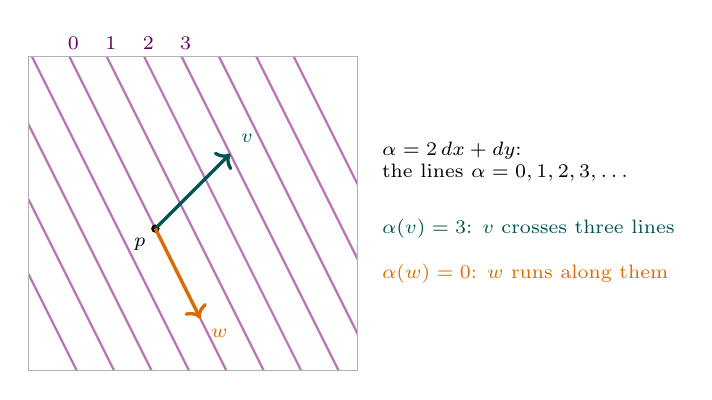
\begin{tikzpicture}[scale=0.95]
\begin{scope}
\clip (-1.7,-1.9) rectangle (2.7,2.3);
\foreach \c in {-4,...,6} \draw[violet!55, thick] ({(\c+2)/2},-2) -- ({(\c-2.4)/2},2.4);
\end{scope}
\draw[gray!60] (-1.7,-1.9) rectangle (2.7,2.3);
\foreach \c in {0,1,2,3} \node[violet!75!black, font=\scriptsize] at ({(\c-2.45)/2+0.13},2.48) {$\c$};
\fill (0,0) circle (1.6pt) node[below left, font=\scriptsize] {$p$};
\draw[->, very thick, teal!65!black] (0,0) -- (1,1) node[above right, font=\scriptsize] {$v$};
\draw[->, very thick, orange!85!black] (0,0) -- (0.6,-1.2) node[below right, font=\scriptsize] {$w$};
\node[font=\scriptsize, align=left, anchor=west] at (2.9,0.9) {$\alpha = 2\,dx + dy$:\\ the lines $\alpha = 0, 1, 2, 3, \ldots$};
\node[font=\scriptsize, align=left, anchor=west, teal!65!black] at (2.9,0.0) {$\alpha(v) = 3$: $v$ crosses three lines};
\node[font=\scriptsize, align=left, anchor=west, orange!85!black] at (2.9,-0.6) {$\alpha(w) = 0$: $w$ runs along them};
\end{tikzpicture}
\end{center}

A covector drawn as a stack of parallel lines. In $\mathbb{R}^2$ (or in one tangent space, after choosing a basis) the covector $\alpha = 2\,dx + dy$ is pictured by its level lines $\{\alpha = 0\}, \{\alpha = 1\}, \ldots$; its value on an arrow is the number of lines the arrow crosses, with sign. $v = \partial_x + \partial_y$ crosses three, so $\alpha(v) = 3$; $w = 0.6\,\partial_x - 1.2\,\partial_y$ runs along the lines, so $\alpha(w) = 0$. For $\alpha = df_p$ the lines are the level sets of the linear approximation of $f$ at $p$: closely spaced lines mean a steep $f$. An arrow and a stack of lines are different kinds of objects; only an inner product turns one into the other.

\textbf{Step 4: the cotangent space from germs alone.} The differential of $f$ depends only on $f$ to first order: $T_p^*M \cong I_p/I_p^2$, the germs vanishing at $p$ modulo those vanishing to second order, by $[[f - f(p)]] \mapsto df_p$ (Theorem~\ref{thm:cotangent-ideal}). So covectors can be built from functions without mentioning tangent vectors at all --- the cotangent space is ``very extremely natural from the point of view of functions'' (Remark~\ref{rem:cotangent-natural}).

\begin{quote}
\textbf{Recall: Definition~\ref{def:Ip-quotient} (The Space $I_p/I_p^2$).} $I_p/I_p^2$ is the quotient vector space (Definition~\ref{def:quotient-vs}) of $I_p$ by its subspace $I_p^2$ (Lemma~\ref{lem:Ip-subspaces}). The class of $[f] \in I_p$ is written $[[f]] = [f] + I_p^2$, and $[[f]] = [[f']]$ iff $[f'] - [f] \in I_p^2$.
\end{quote}

\begin{quote}
\textbf{Recall: Theorem~\ref{thm:cotangent-ideal} (The Cotangent Space from Germs).} \begin{enumerate}
    \item The pairing induces isomorphisms
    \[
    T_pM \xrightarrow{\ \cong\ } \big(I_p/I_p^2\big)^*, \qquad\qquad \Phi : I_p/I_p^2 \xrightarrow{\ \cong\ } (T_pM)^* = T_p^*M .
    \]
    \item $\Phi([[f]]) = df_p$: the isomorphism sends the class of a germ to its differential.
    \item In any chart, $\Phi$ carries the basis $[[x^i - x^i(p)]]$ of $I_p/I_p^2$ to the basis $dx^i|_p$ of $T_p^*M$, which is dual to the basis $\partial/\partial x^i|_p$ of $T_pM$.
\end{enumerate}
The isomorphisms are defined without any chart.
\end{quote}

\textbf{Step 5: covectors pull back.} For $F : M \to N$, the dual map of $F_{*p}$ is the \emph{pullback of covectors} $F_p^* : T^*_{F(p)}N \to T_p^*M$, $(F_p^*\alpha)(v) = \alpha(F_{*p}v)$ (Definition~\ref{def:pullback-covector}). It commutes with differentials: $F_p^*(df_{F(p)}) = d(f \circ F)_p$ (Proposition~\ref{prop:pullback-d}), which is the chain rule in covector form. The same symbol $F_p^*$ already denoted the pullback of germs (Step~5 of \ref{sec:recap-tangent}); the two are compatible, as Remark~\ref{rem:two-pullbacks} explains.

\begin{quote}
\textbf{Recall: Definition~\ref{def:pullback-covector} (Pullback of Covectors).} Let $F : M \to N$ be smooth and $p \in M$. The \textbf{pullback of covectors} at $p$ is the dual map (Definition~\ref{def:dual-map}) of the pushforward $F_{*p} : T_pM \to T_{F(p)}N$:
\[
F_p^* : T^*_{F(p)}N \longrightarrow T_p^*M, \qquad (F_p^*\alpha)(v) = \alpha\big(F_{*p}v\big) .
\]
\end{quote}

\begin{quote}
\textbf{Recall: Proposition~\ref{prop:pullback-d} (Pullback Commutes with $d$).} Let $F : M \to N$ be smooth, $p \in M$, and $f$ smooth near $F(p)$. Then
\[
F_p^*\big(df_{F(p)}\big) = d(f \circ F)_p \quad \text{in } T_p^*M .
\]
\end{quote}

\textbf{Step 6: the word ``differential''.} The course uses it for four objects. They are one idea at four levels of generality.

\begin{center}
\renewcommand{\arraystretch}{1.3}
\begin{tabular}{p{0.25\textwidth} p{0.13\textwidth} p{0.27\textwidth} p{0.25\textwidth}}
\hline
Name & Symbol & Takes \ldots\ to \ldots & Defined in \\
\hline
differential of a map between vector spaces & $dF_p$ & a vector in $X$ to a vector in $Y$ (the Jacobian) & Definition~\ref{def:vs-differential} \\
differential (pushforward) of a smooth map & $F_{*p}$ & $T_pM \to T_{F(p)}N$ & Definition~\ref{def:pushforward} \\
differential of a function at $p$ & $df_p$ & $T_pM \to \mathbb{R}$, a covector & Definition~\ref{def:differential-function} \\
the operator $d$ & $d$ & a function $f$ to the one-form $df$ & Proposition~\ref{prop:d-operator} \\
\hline
\end{tabular}
\end{center}

How they fit: on open subsets of $\mathbb{R}^n$ the second is the first (Proposition~\ref{prop:differential-agree}); Lee writes $dF_p$ for what these notes call $F_{*p}$, and Uribe said in Lecture~15 that $F_{*p}$ ``we should have called the differential of $F$ ages ago''. The third is the second for maps into $\mathbb{R}$. The fourth collects the third over all points: $df$ is the field $p \mapsto df_p$, a one-form (\ref{sec:d-operator}).

\textbf{Step 7: forward and backward.} Given $F : M \to N$:

\begin{center}
\renewcommand{\arraystretch}{1.3}
\begin{tabular}{p{0.27\textwidth} p{0.14\textwidth} p{0.48\textwidth}}
\hline
Object & Moves & Rule \\
\hline
point $p \in M$ & forward & $p \mapsto F(p)$ \\
tangent vector $v \in T_pM$ & forward & $F_{*p}v \in T_{F(p)}N$ (Definition~\ref{def:pushforward}) \\
function $f$ on $N$ & backward & $F^*f = f \circ F$ on $M$ \\
germ $[g]$ at $F(p)$ & backward & $F_p^*[g] = [g \circ F]$ (Definition~\ref{def:germ-pullback}) \\
covector $\alpha \in T^*_{F(p)}N$ & backward & $(F_p^*\alpha)(v) = \alpha(F_{*p}v)$ (Definition~\ref{def:pullback-covector}) \\
\hline
\end{tabular}
\end{center}

Things that \emph{are} somewhere move forward with the points; things that \emph{eat} move backward, because to evaluate one on $M$ you push its input forward and evaluate on $N$.

\textbf{What this chapter builds.} So far every object lives at a single point. This chapter lets the point vary. The tangent spaces are assembled into one manifold, the tangent bundle $TM$ (\ref{sec:tangent-bundle}), and the cotangent spaces into the cotangent bundle $T^*M$ (\ref{sec:cotangent-bundle}). A smooth choice of a covector at every point is a one-form; $d$ turns functions into one-forms, and $F^*$ pulls one-forms back (\ref{sec:d-operator}). A smooth choice of a tangent vector at every point is a vector field, and a vector field differentiates functions everywhere at once (\ref{sec:fields}).

\begin{exbox}[Covectors in the Plane]\exlabel{ex:recap-covectors-plane}
Continue Example~\ref{ex:recap-vectors-plane}: $p = (1, 2)$, $f = x^2 y$, $v = 3\,\partial_x - \partial_y$, and $F(x, y) = (x^2, x + y)$ with $F(p) = (1, 3)$ and $F_{*p}v = 6\,\partial_u + 2\,\partial_w$.
\begin{enumerate}
    \item \emph{The differential of $f$.} $df_p = \partial_x f(p)\, dx + \partial_y f(p)\, dy = 4\, dx + dy$, and $df_p(v) = 4 \cdot 3 + 1 \cdot (-1) = 11 = v[f]$, as Step~3 promises.
    \item \emph{A covector at $F(p)$.} Let $g(u, w) = u w^2$ on the target. Then $dg_{F(p)} = w^2\, du + 2uw\, dw = 9\, du + 6\, dw$ at $(1, 3)$.
    \item \emph{Its pullback, by definition.} $(F_p^* dg_{F(p)})(v) = dg_{F(p)}(F_{*p}v) = 9 \cdot 6 + 6 \cdot 2 = 66$.
    \item \emph{Its pullback, by the chain rule.} $g \circ F = x^2 (x + y)^2$, with $\partial_x (g \circ F)(p) = 2x(x+y)^2 + 2x^2(x+y) = 18 + 6 = 24$ and $\partial_y (g \circ F)(p) = 2x^2(x+y) = 6$. So $d(g \circ F)_p = 24\, dx + 6\, dy$, and $d(g \circ F)_p(v) = 72 - 6 = 66$: the two agree, as Proposition~\ref{prop:pullback-d} says.
    \item \emph{The transpose.} The components of $F_p^*$ come from the \emph{transpose} of the Jacobian: $\begin{pmatrix} 2 & 1 \\ 0 & 1 \end{pmatrix} \begin{pmatrix} 9 \\ 6 \end{pmatrix} = \begin{pmatrix} 24 \\ 6 \end{pmatrix}$. Vectors are pushed forward by the Jacobian, covectors pulled back by its transpose.
\end{enumerate}
\end{exbox}


% ============================================================================
% SECTION: THE TANGENT BUNDLE
% ============================================================================

\section{The Tangent Bundle}\label{sec:tangent-bundle}

\roadmark{Stage: bundles}{All the tangent spaces of $M$, assembled into a single manifold that fibres over $M$.}

\textit{Lecture 12. ``Again, these constructions, especially the cotangent [bundle], are basic parts of the basic theory.'' The tangent bundle was introduced as a set, with its projection and zero section; its topology, smooth structure and charts come next lecture.}

\begin{defbox}[The Tangent Bundle as a Set]\deflabel{def:tangent-bundle-set}
Let $M$ be a smooth manifold of dimension $m$. Its \textbf{tangent bundle} is the set
\[
TM = \bigcup_{p \in M} \{p\} \times T_pM = \{\, (p, v) : p \in M,\ v \in T_pM \,\},
\]
all the tangent spaces ``put together in one big set.'' It comes with the \textbf{projection} $\pi : TM \to M$, $\pi(p, v) = p$, whose fibre $\pi^{-1}(p) = \{p\} \times T_pM$ is identified with $T_pM$; and with the \textbf{zero section} $\zeta : M \to TM$, $\zeta(p) = (p, 0)$, which is one-to-one because every tangent space has a distinguished element, its zero.
\leeref{Ch.~3, \emph{The Tangent Bundle}}
\end{defbox}

\begin{rembox}[The Picture Changes]\label{rem:picture-changes}
``There are several psychological inflection steps that one needs to make. The most important one is that we're going to think of $TM$ as fibering over $M$.'' A tangent space is usually drawn touching $M$, lying along it. In the bundle picture it stands \emph{vertically}, as the fibre over its point, and $M$ itself sits horizontally inside $TM$ as the zero section --- the tangent spaces become ``transversal'' to it.
\end{rembox}

\begin{center}
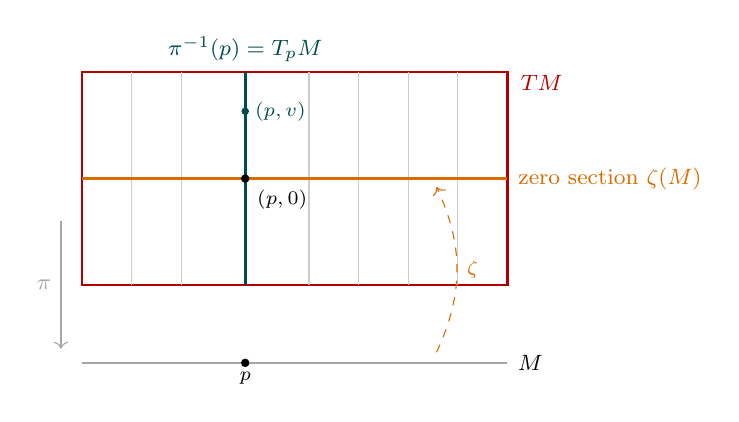
\begin{tikzpicture}[scale=0.9]
\draw[red!70!black, thick] (0,-1.5) rectangle (6,1.5); \node[red!70!black, font=\footnotesize, anchor=south west] at (6.05,1.1) {$TM$};
\draw[gray!40] (0.70,-1.5) -- (0.70,1.5);
\draw[gray!40] (1.40,-1.5) -- (1.40,1.5);
\draw[gray!40] (3.20,-1.5) -- (3.20,1.5);
\draw[gray!40] (3.90,-1.5) -- (3.90,1.5);
\draw[gray!40] (4.60,-1.5) -- (4.60,1.5);
\draw[gray!40] (5.30,-1.5) -- (5.30,1.5);
\draw[teal!60!black, very thick] (2.3,-1.5) -- (2.3,1.5) node[above, font=\footnotesize] {$\pi^{-1}(p) = T_pM$};
\draw[orange!85!black, very thick] (0,0) -- (6,0) node[right, font=\footnotesize] {zero section $\zeta(M)$};
\fill (2.3,0) circle (1.7pt); \node[font=\scriptsize, anchor=north west] at (2.33,-0.02) {$(p, 0)$};
\fill[teal!60!black] (2.3,0.95) circle (1.5pt) node[right, font=\scriptsize] {$(p, v)$};
\draw[thick, gray!70] (0,-2.6) -- (6,-2.6) node[right, font=\footnotesize, text=black] {$M$};
\fill (2.3,-2.6) circle (1.7pt) node[below, font=\scriptsize] {$p$};
\draw[->, gray!70] (-0.3,-0.6) -- node[left, font=\footnotesize] {$\pi$} (-0.3,-2.4);
\draw[->, dashed, orange!85!black] (5.0,-2.45) to[bend right=25] node[right, font=\scriptsize] {$\zeta$} (5.0,-0.12);
\end{tikzpicture}
\end{center}

The tangent bundle as a fibration. Each fibre $\pi^{-1}(p) = T_pM$ is a vertical line over $p$ (in general a copy of $\mathbb{R}^m$); the point $(p, v)$ lies on it, and the zero section $\zeta$ lifts each $p$ straight up to $(p, 0)$, placing a copy of $M$ horizontally inside $TM$.


\textit{Status.} Proposition~\ref{prop:tangent-bundle-claim}, below, was stated in Lecture~12 --- ``the claim, which takes a lot of detail to prove'' --- and made precise in Lecture~13 (\ref{sub:tb-charts}), which wrote down the charts. Their idea was given: a chart $(U, \varphi = (x^1, \ldots, x^m))$ of $M$ gives the basis $\partial/\partial x^i|_p$ of every $T_pM$, $p \in U$, hence an identification of each of these tangent spaces with $\mathbb{R}^m$; ``putting all that together gives us a map'' $\pi^{-1}(U) \to \varphi(U) \times \mathbb{R}^m \subseteq \mathbb{R}^{2m}$, the chart of $TM$. The dimension $2m$ is $m$ coordinates for the point and $m$ for the vector.

\subsection{Trivializations and Charts}\label{sub:tb-charts}

\textit{Lecture 13. ``Back to the tangent bundle.'' $TM$ has been defined as a set; its charts come from charts of $M$ and the coordinate bases.}

\begin{defbox}[Local Trivializations of $TM$]\deflabel{def:tb-charts}
Let $(U, \varphi = (x^1, \ldots, x^m))$ be a smooth chart of $M$, and $TU = \pi^{-1}(U) = \{(p, v) \in TM : p \in U\}$, the tangent vectors at points of $U$. The \textbf{local trivialization} over $U$ is
\[
\Phi : TU \longrightarrow U \times \mathbb{R}^m, \qquad \Phi(p, v) = (p, v^1, \ldots, v^m), \qquad \text{where } v = \sum_{i=1}^m v^i \frac{\partial}{\partial x^i}\Big|_p ,
\]
the components of $v$ in the coordinate basis (Theorem~\ref{thm:tangent-basis}). It is a bijection, and $\mathrm{pr}_1 \circ \Phi = \pi$ --- ``that's why I call it a trivialization.''
\leeref{Proposition 3.18}
\end{defbox}

\begin{defbox}[Charts of $TM$]\deflabel{def:tb-chart}
Let $(U, \varphi = (x^1, \ldots, x^m))$ be a smooth chart of $M$ and $\Phi$ the local trivialization over $U$ (Definition~\ref{def:tb-charts}). The \textbf{chart} of $TM$ over $U$ is
\[
\tilde\varphi = (\varphi \times \mathrm{id}) \circ \Phi : TU \longrightarrow \varphi(U) \times \mathbb{R}^m \subseteq \mathbb{R}^{2m}, \qquad (p, v) \longmapsto \big(x^1(p), \ldots, x^m(p), v^1, \ldots, v^m\big).
\]
It is a bijection, with inverse $(r, v) \mapsto \big(\varphi^{-1}(r), \sum_i v^i\, \partial/\partial x^i|_{\varphi^{-1}(r)}\big)$.
\leeref{Proposition 3.18}
\end{defbox}

\begin{center}
\begin{tikzcd}[column sep=4.6em, row sep=3em]
TU \arrow[r, "\Phi"] \arrow[dr, "\pi"'] \arrow[rr, bend left=28, "\tilde\varphi"] & U \times \mathbb{R}^m \arrow[r, "\varphi \times \mathrm{id}"] \arrow[d, "\mathrm{pr}_1"] & \varphi(U) \times \mathbb{R}^m \subseteq \mathbb{R}^{2m} \\
& U &
\end{tikzcd}
\end{center}

The trivialization and the chart, as on the board. The triangle commutes, $\mathrm{pr}_1 \circ \Phi = \pi$ --- the fibration diagram of Definition~\ref{def:fibration} --- and the chart $\tilde\varphi$ is $\Phi$ followed by $\varphi$ on the first factor.

\begin{propbox}[The Topology of $TM$]\thmlabel{prop:tb-topology}
There is a unique topology on $TM$ for which every $TU$ is open and every chart $\tilde\varphi : TU \to \varphi(U) \times \mathbb{R}^m$ is a homeomorphism. With it, $TM$ is a topological manifold of dimension $2m$.
\leeref{Lemma 1.35 and Proposition 3.18}
\end{propbox}

\begin{proof}
\textit{(Stated in Lecture~13 without proof --- ``it's all point-set topology, and of course everything is in Lee \ldots\ see Lee''; filled in, following Lee's smooth manifold chart lemma.)} Throughout, $(U, \varphi)$ and $(V, \psi)$ denote smooth charts of $M$.

\emph{The transition maps.} The computation in the proof of Proposition~\ref{prop:tb-atlas} below uses only the definitions of the charts, not any topology on $TM$. It shows that $\tilde\psi \circ \tilde\varphi^{-1}$ maps the open set $\tilde\varphi(TU \cap TV) = \varphi(U \cap V) \times \mathbb{R}^m$ bijectively onto the open set $\psi(U \cap V) \times \mathbb{R}^m$, by a smooth map whose inverse, $\tilde\varphi \circ \tilde\psi^{-1}$, is given by the same formula with the two charts exchanged. So each transition map is a homeomorphism between open subsets of $\mathbb{R}^{2m}$.

\emph{The topology.} Declare $W \subseteq TM$ open if $\tilde\varphi(W \cap TU)$ is open in $\mathbb{R}^{2m}$ for every chart $(U, \varphi)$. This is a topology: $\emptyset$ and $TM$ are open, the latter because $\tilde\varphi(TU) = \varphi(U) \times \mathbb{R}^m$ is open; and since each $\tilde\varphi$ is a bijection, it carries unions and finite intersections of subsets of $TU$ to unions and finite intersections of their images.

\emph{Each $TU$ is open, and each $\tilde\varphi$ is a homeomorphism onto an open set.} For any chart $(V, \psi)$, $\tilde\psi(TU \cap TV) = \psi(U \cap V) \times \mathbb{R}^m$ is open, so $TU$ is open. If $W \subseteq TU$ is open, then $\tilde\varphi(W) = \tilde\varphi(W \cap TU)$ is open by definition, so $\tilde\varphi$ is an open map. For continuity, let $O \subseteq \varphi(U) \times \mathbb{R}^m$ be open and $W = \tilde\varphi^{-1}(O)$. For any chart $(V, \psi)$,
\[
\tilde\psi(W \cap TV) = \big(\tilde\psi \circ \tilde\varphi^{-1}\big)\Big(O \cap \big(\varphi(U \cap V) \times \mathbb{R}^m\big)\Big),
\]
the image of an open set under a homeomorphism between open sets, hence open. So $W$ is open.

\emph{Uniqueness.} Let $\tau'$ be any topology in which every $TU$ is open and every $\tilde\varphi$ is a homeomorphism. If $W \in \tau'$, then $W \cap TU$ is open in $TU$, so $\tilde\varphi(W \cap TU)$ is open, and $W$ is open in the topology above. Conversely, if $W$ is open above, then each $W \cap TU = \tilde\varphi^{-1}\big(\tilde\varphi(W \cap TU)\big)$ is open in $TU$, hence in $\tau'$ since $TU \in \tau'$, and $W = \bigcup_U (W \cap TU) \in \tau'$.

\emph{Locally Euclidean.} Every point of $TM$ lies in some $TU$, which is open and homeomorphic, by $\tilde\varphi$, to an open subset of $\mathbb{R}^{2m}$.

\emph{Hausdorff.} Let $(p, v) \ne (q, w)$. If $p = q$, both points lie in one $TU$, homeomorphic to a subset of the Hausdorff space $\mathbb{R}^{2m}$; disjoint open sets of $TU$ separating them are open in $TM$, because $TU$ is. If $p \ne q$, choose charts with disjoint domains $U \ni p$ and $V \ni q$, possible because $M$ is Hausdorff (shrink the domains, Lemma~\ref{lem:chart-modify}); then $TU$ and $TV$ are disjoint open sets containing the two points.

\emph{Second countable.} Let $\mathcal{B}$ be a countable basis of $M$. For each $B \in \mathcal{B}$ contained in some chart domain, choose one such chart $(U_B, \varphi_B)$. These countably many charts cover $M$: each $p$ lies in some chart domain $U$, and then in some $B \in \mathcal{B}$ with $p \in B \subseteq U$. So the countably many open sets $TU_B$ cover $TM$. Each is homeomorphic to an open subset of $\mathbb{R}^{2m}$, so has a countable basis, whose members are open in $TM$; the union of these countably many bases is countable and is a basis of $TM$, since any open $W \ni (p, v)$ meets some $TU_B$ containing $(p, v)$ in a set open in $TU_B$.
\end{proof}

The same argument, word for word, builds the topology of the cotangent bundle (\ref{sub:cotangent-bundle}), with the dual bases in place of the coordinate bases.

\begin{propbox}[The Smooth Atlas of $TM$]\thmlabel{prop:tb-atlas}
The charts $(TU, \tilde\varphi)$, as $(U, \varphi)$ ranges over the smooth charts of $M$, form a smooth atlas on $TM$. For charts $\varphi = (x^i)$ and $\psi = (y^j)$ of $M$, the transition map is
\[
\tilde\psi \circ \tilde\varphi^{-1}(r, v) = \Big( \psi \circ \varphi^{-1}(r), \ \ \sum_{j=1}^m \frac{\partial y^1}{\partial x^j}\big(\varphi^{-1}(r)\big)\, v^j, \ \ldots, \ \sum_{j=1}^m \frac{\partial y^m}{\partial x^j}\big(\varphi^{-1}(r)\big)\, v^j \Big) .
\]
\leeref{Proposition 3.18}
\end{propbox}

\begin{proof}
\textit{(Lecture~13: ``the only thing that I want to have a look at is \ldots\ the transition functions of the atlas, because this is how people handle tangent vectors.'' Completed here.)} The domain is $\tilde\varphi(TU \cap TV) = \varphi(U \cap V) \times \mathbb{R}^m$, open in $\mathbb{R}^{2m}$. Let $p \in U \cap V$ and $v \in T_pM$, written in both bases:
\[
v = \sum_j v^j \frac{\partial}{\partial x^j}\Big|_p = \sum_i w^i \frac{\partial}{\partial y^i}\Big|_p .
\]
The first component of the transition is $\psi \circ \varphi^{-1}$, smooth because the charts of $M$ are compatible. For the rest we need the $w$'s in terms of the $v$'s: ``a change of basis formula from 217, which I always forget.'' By the universal formula (Theorem~\ref{thm:tangent-basis}), the $i$-th coefficient of a derivation $D$ in the basis $\partial/\partial y^i|_p$ is $D[y^i]$; applied to $D = \partial/\partial x^j|_p$ it gives
\[
\frac{\partial}{\partial x^j}\Big|_p = \sum_i \frac{\partial y^i}{\partial x^j}(p) \frac{\partial}{\partial y^i}\Big|_p, \qquad\text{so}\qquad w^i = \sum_j \frac{\partial y^i}{\partial x^j}(p)\, v^j ,
\]
comparing coefficients in the basis $\partial/\partial y^i|_p$. (In lecture Uribe expanded $\partial/\partial y^j$ in the other basis and first solved for the $v$'s --- ``I did it backwards'' --- then took the other direction ``by the same argument''.) With $p = \varphi^{-1}(r)$ this is the displayed formula. The coefficients are smooth functions of $r$: by Proposition~\ref{prop:upstairs-downstairs}, $\partial y^i/\partial x^j(\varphi^{-1}(r)) = \partial(\psi \circ \varphi^{-1})^i/\partial r^j(r)$, the entries of the Jacobian of the transition map of $M$. So the transition map of $TM$ is $(r, v) \mapsto \big(\psi \circ \varphi^{-1}(r), (\psi \circ \varphi^{-1})'(r)\, v\big)$, smooth.
\end{proof}

\begin{center}
\begin{tikzcd}[column sep=5.4em, row sep=3em]
& TU \cap TV \arrow[dl, "\tilde\varphi"'] \arrow[dr, "\tilde\psi"] & \\
\varphi(U \cap V) \times \mathbb{R}^m \arrow[rr, "{(r, v) \,\mapsto\, (\psi \circ \varphi^{-1}(r),\ (\psi \circ \varphi^{-1})'(r)\, v)}"'] & & \psi(U \cap V) \times \mathbb{R}^m
\end{tikzcd}
\end{center}

The transition map of the charts $\tilde\varphi$ and $\tilde\psi$ of $TM$, as drawn in lecture over a point $(p, v)$ of $TU \cap TV$.

The transition map of $TM$, in one line: the base point moves by the transition map of $M$, and the vector by its Jacobian. This is Uribe's identity at work once more --- the partials $\partial y^i/\partial x^j$, taken upstairs on $M$, are the Jacobian downstairs.

\begin{corbox}[The Tangent Bundle Is a Fibration]\thmlabel{cor:tb-fibration}
With the smooth structure of Proposition~\ref{prop:tb-atlas}:
\begin{enumerate}
    \item $TM$ is a smooth manifold of dimension $2m$, and $\pi : TM \to M$ is smooth;
    \item the $\Phi$ are local trivializations, so $\pi$ is a fibration with fibre $\mathbb{R}^m$, and each $\Phi$ restricts on the fibre $T_pM$ to a linear isomorphism $T_pM \to \{p\} \times \mathbb{R}^m$;
    \item the image $\zeta(M)$ of the zero section is a submanifold of $TM$ of codimension $m$.
\end{enumerate}
With Proposition~\ref{prop:tb-topology}, this proves Proposition~\ref{prop:tangent-bundle-claim} below in full.
\end{corbox}

\begin{proof}
\textit{((1) and (2) are the lecture's observations --- ``in these coordinates, the projection is just projection onto the first $m$ components \ldots\ so we get a beautiful fibration''; the details and (3) are filled in.)} (1) In the charts $\tilde\varphi$ and $\varphi$, $\pi$ is $(r, v) \mapsto r$, which is smooth. (2) $\Phi = (\varphi^{-1} \times \mathrm{id}) \circ \tilde\varphi$ is a composite of diffeomorphisms (Proposition~\ref{prop:chart-diffeo}), and $\mathrm{pr}_1 \circ \Phi = \pi$; the $TU$ cover $TM$, the $U$ cover $M$. On $T_pM$, $\Phi$ is $v \mapsto (p, v^1, \ldots, v^m)$, taking components in a basis, which is a linear isomorphism. (3) In the chart $\tilde\varphi$, $\zeta(M) \cap TU = \{v^1 = \cdots = v^m = 0\}$, so the charts $\tilde\varphi$ are adapted to $\zeta(M)$ (Definition~\ref{def:submanifold}).
\end{proof}
\begin{propbox}[The Tangent Bundle Is a Manifold (Claim)]\thmlabel{prop:tangent-bundle-claim}
$TM$ has a natural topology and smooth structure making it a smooth manifold of dimension $2m$, for which $\pi : TM \to M$ is a fibration with fibre $\mathbb{R}^m$, and the image $\zeta(M)$ of the zero section is a submanifold of $TM$.
\leeref{Proposition 3.18}
\end{propbox}

\begin{proof}[Proof]
Proposition~\ref{prop:tb-topology} gives the topology, and Corollary~\ref{cor:tb-fibration} the smooth structure, the fibration with fibre $\mathbb{R}^m$, and the zero section as a submanifold.
\end{proof}

\begin{rembox}[Vector Bundles]\label{rem:vector-bundles}
$TM$ is in fact a \emph{vector bundle}: a fibration whose fibres are vector spaces, with trivializations that are linear isomorphisms on each fibre. Uribe postponed the general definition --- ``it takes another 10 minutes of axioms'' --- but these are the two features: ``the fibres are abstract vector spaces, and you can find trivializations which restrict to linear isomorphisms fibrewise.'' Vector bundles are ``fun objects'' in their own right; K-theory is built from them.
\end{rembox}

\begin{rembox}[Trivializations and Frames]\label{rem:same-principle-elsewhere}
Proposition~\ref{prop:trivialization-section} turns local trivializations into local sections. For the tangent bundle the dictionary is between trivializations and \emph{frames}: the trivialization $\Phi$ of a chart (Definition~\ref{def:tb-charts}) corresponds to the $m$ local sections $u \mapsto \partial/\partial x^i|_u$, since $\Phi^{-1}(u, e_i) = \partial/\partial x^i|_u$; for a vector bundle of rank $m$ one local section is not enough, and it takes $m$ sections that are linearly independent at every point (Lee, Example~10.18 and Proposition~10.19). For the Hopf fibration one section suffices because the fibre is a single orbit of the free $S^1$-action. That is the general pattern of \emph{principal bundles}, where a group acts freely and transitively on each fibre; it is stated here, not proved.
\end{rembox}

% ============================================================================
% SECTION: THE COTANGENT BUNDLE
% ============================================================================

\section{The Cotangent Bundle}\label{sec:cotangent-bundle}\label{sub:cotangent-bundle}

\roadmark{Stage: bundles}{The cotangent spaces assembled into $T^*M$, with charts from the dual bases; covector components transform by the inverse transpose.}

\textit{Lecture 13 defined the cotangent bundle --- ``completely analogous'' to the tangent bundle, with the dual bases in place of the coordinate bases; Lecture 15 returned to it for the homework.}

\begin{defbox}[The Cotangent Bundle as a Set]\deflabel{def:cotangent-bundle}
Let $M$ be a smooth manifold of dimension $m$. Its \textbf{cotangent bundle} is the set
\[
T^*M = \bigcup_{p \in M} \{p\} \times T_p^*M = \{\, (p, \xi) : p \in M,\ \xi \in T_p^*M \,\},
\]
all the cotangent spaces (Definition~\ref{def:cotangent}) put together. It comes with the \textbf{projection} $\pi : T^*M \to M$, $\pi(p, \xi) = p$, whose fibre $\pi^{-1}(p) = \{p\} \times T_p^*M$ is identified with $T_p^*M$; and with the \textbf{zero section} $\zeta : M \to T^*M$, $\zeta(p) = (p, 0)$.
\leeref{Ch.~11, \emph{The Cotangent Bundle}}
\end{defbox}

The definitions and results of this section run parallel to those for the tangent bundle in \ref{sec:tangent-bundle}, item for item, with the dual bases $dx^i|_p$ in place of the coordinate bases $\partial/\partial x^i|_p$. Lecture~13 gave the charts and the transition maps; the rest is filled in, following Section~\ref{sec:tangent-bundle}.

\subsection{Trivializations and Charts}\label{sub:ctb-charts}

\begin{defbox}[Local Trivializations of $T^*M$]\deflabel{def:ctb-trivialization}
Let $(U, \varphi = (x^1, \ldots, x^m))$ be a smooth chart of $M$, and $T^*U = \pi^{-1}(U) = \{(p, \xi) \in T^*M : p \in U\}$, the covectors at points of $U$. The \textbf{local trivialization} of $T^*M$ over $U$ is
\[
\Psi : T^*U \longrightarrow U \times \mathbb{R}^m, \qquad \Psi(p, \xi) = (p, \xi_1, \ldots, \xi_m), \qquad \text{where } \xi = \sum_{i=1}^m \xi_i\, dx^i\big|_p ,
\]
the components of $\xi$ in the dual basis. Because the bases $dx^i|_p$ and $\partial/\partial x^i|_p$ are dual to each other, the components are computed by evaluation, $\xi_i = \xi\big(\partial/\partial x^i|_p\big)$ (Corollary~\ref{cor:covector-components}). $\Psi$ is a bijection, and $\mathrm{pr}_1 \circ \Psi = \pi$.
\leeref{Proposition 11.9}
\end{defbox}

\begin{defbox}[Charts of $T^*M$]\deflabel{def:ctb-chart}
Let $(U, \varphi = (x^1, \ldots, x^m))$ be a smooth chart of $M$ and $\Psi$ the local trivialization over $U$ (Definition~\ref{def:ctb-trivialization}). The \textbf{chart} of $T^*M$ over $U$ --- the \textbf{standard coordinates} on $T^*U$ --- is
\[
\hat\varphi = (\varphi \times \mathrm{id}) \circ \Psi : T^*U \longrightarrow \varphi(U) \times \mathbb{R}^m \subseteq \mathbb{R}^{2m}, \qquad (p, \xi) \longmapsto \big(x^1(p), \ldots, x^m(p), \xi_1, \ldots, \xi_m\big).
\]
It is a bijection, with inverse $(r, \xi) \mapsto \big(\varphi^{-1}(r), \sum_i \xi_i\, dx^i|_{\varphi^{-1}(r)}\big)$.
\leeref{Proposition 11.9}
\end{defbox}

\begin{propbox}[The Topology of $T^*M$]\thmlabel{prop:ctb-topology}
There is a unique topology on $T^*M$ for which every $T^*U$ is open and every chart $\hat\varphi : T^*U \to \varphi(U) \times \mathbb{R}^m$ is a homeomorphism. With it, $T^*M$ is a topological manifold of dimension $2m$.
\leeref{Lemma 1.35 and Proposition 11.9}
\end{propbox}

\begin{proof}
\textit{(Not from lecture --- ``completely analogous''; filled in.)} The proof of Proposition~\ref{prop:tb-topology} uses only two facts about the charts $\tilde\varphi$: each is a bijection of $TU$ onto the open set $\varphi(U) \times \mathbb{R}^m$, and each transition map $\tilde\psi \circ \tilde\varphi^{-1}$ is a homeomorphism between the open sets $\varphi(U \cap V) \times \mathbb{R}^m$ and $\psi(U \cap V) \times \mathbb{R}^m$. Both hold for the charts $\hat\varphi$: the first by Definition~\ref{def:ctb-chart}, and the second by the computation in the proof of Proposition~\ref{prop:cotangent-transition} below, which uses only the definitions of the charts, not any topology on $T^*M$. With $\hat\varphi$, $\hat\psi$ and $T^*U$ in place of $\tilde\varphi$, $\tilde\psi$ and $TU$, the proof then goes through word for word:
\begin{itemize}
    \item declare $W \subseteq T^*M$ open if $\hat\varphi(W \cap T^*U)$ is open in $\mathbb{R}^{2m}$ for every chart $(U, \varphi)$; this is a topology, since each $\hat\varphi$ is a bijection;
    \item each $T^*U$ is open, because $\hat\psi(T^*U \cap T^*V) = \psi(U \cap V) \times \mathbb{R}^m$ is open, and each $\hat\varphi$ is a homeomorphism onto its open image, because the transition maps are homeomorphisms;
    \item any topology with these two properties has the same open sets, since $W = \bigcup_U (W \cap T^*U)$;
    \item $T^*M$ is locally Euclidean of dimension $2m$, through the charts;
    \item it is Hausdorff: two covectors at the same point lie in one $T^*U$, homeomorphic to a subset of $\mathbb{R}^{2m}$, and covectors at distinct points $p \neq q$ lie in the disjoint open sets $T^*U$, $T^*V$ for charts with disjoint domains $U \ni p$, $V \ni q$;
    \item it is second countable: countably many chart domains $U_B$ cover $M$, so the countably many open sets $T^*U_B$, each with a countable basis, cover $T^*M$.
\end{itemize}
\end{proof}

\begin{propbox}[The Smooth Atlas of $T^*M$]\thmlabel{prop:cotangent-transition}
The charts $(T^*U, \hat\varphi)$, as $(U, \varphi)$ ranges over the smooth charts of $M$, form a smooth atlas on $T^*M$. For charts $\varphi = (x^i)$ and $\psi = (y^j)$, if $\xi = \sum_i \xi_i\, dx^i|_p = \sum_j \eta_j\, dy^j|_p$, then
\[
dx^i|_p = \sum_j \frac{\partial x^i}{\partial y^j}(p)\, dy^j|_p, \qquad \eta_j = \sum_i \frac{\partial x^i}{\partial y^j}(p)\, \xi_i .
\]
So the covector components transform by the transpose of the inverse of the matrix that transforms tangent components: with $\tau = \psi \circ \varphi^{-1}$, the transition map is
\[
\hat\psi \circ \hat\varphi^{-1}(r, \xi) = \Big( \tau(r),\ \big(\tau'(r)^{-1}\big)^{\mathsf T} \xi \Big) .
\]
\leeref{Proposition 11.9}
\end{propbox}

\begin{proof}
\textit{(Lecture~13: ``completely analogous'', with the change ``we use the dual basis'', and the formula for $dx^i$ given; the rest is filled in.)} The formula for $dx^i|_p$ is Lemma~\ref{lem:df-coords} applied to the function $x^i$ in the chart $\psi$. Substituting it into $\sum_i \xi_i\, dx^i|_p$ and comparing coefficients of $dy^j|_p$ gives $\eta_j$. The matrix $\big[\partial x^i/\partial y^j\big]$ is the inverse of $\big[\partial y^i/\partial x^j\big]$ (chain rule), so the tangent components transform by $A = \big[\partial y^i/\partial x^j\big]$ and the covector components by $(A^{-1})^{\mathsf T}$. Its entries are smooth functions of the base point, so the transition maps are smooth, as in Proposition~\ref{prop:tb-atlas}; the fibration and linearity statements follow as in Corollary~\ref{cor:tb-fibration}.
Explicitly, with $p = \varphi^{-1}(r)$, the matrix $\big[\partial y^i/\partial x^j(p)\big]$ is $\tau'(r)$ (Proposition~\ref{prop:upstairs-downstairs}), so $\big[\partial x^i/\partial y^j(p)\big] = \tau'(r)^{-1}$ and $\eta = \big(\tau'(r)^{-1}\big)^{\mathsf T}\xi$, which is the displayed transition map. Its entries are smooth in $r$: those of $\tau'(r)$ are, and the inverse of an invertible matrix is given by Cramer's rule, a quotient of polynomials in the entries by the nonzero determinant. The inverse transition map is the same formula with the two charts exchanged.
\end{proof}

\begin{corbox}[The Cotangent Bundle Is a Fibration]\thmlabel{cor:ctb-fibration}
With the smooth structure of Proposition~\ref{prop:cotangent-transition}:
\begin{enumerate}
    \item $T^*M$ is a smooth manifold of dimension $2m$, and $\pi : T^*M \to M$ is smooth;
    \item the $\Psi$ are local trivializations, so $\pi$ is a fibration with fibre $\mathbb{R}^m$, and each $\Psi$ restricts on the fibre $T_p^*M$ to a linear isomorphism $T_p^*M \to \{p\} \times \mathbb{R}^m$; so $T^*M$ is a vector bundle;
    \item the image $\zeta(M)$ of the zero section is a submanifold of $T^*M$ of codimension $m$.
\end{enumerate}
\leeref{Proposition 11.9}
\end{corbox}

\begin{proof}
\textit{(Not from lecture; filled in, as Corollary~\ref{cor:tb-fibration}.)} (1) By Propositions~\ref{prop:ctb-topology} and~\ref{prop:cotangent-transition}. In the charts $\hat\varphi$ and $\varphi$, $\pi$ is $(r, \xi) \mapsto r$, which is smooth. (2) $\Psi = (\varphi^{-1} \times \mathrm{id}) \circ \hat\varphi$ is a composite of diffeomorphisms (Proposition~\ref{prop:chart-diffeo}), and $\mathrm{pr}_1 \circ \Psi = \pi$; the $T^*U$ cover $T^*M$ and the $U$ cover $M$. On $T_p^*M$, $\Psi$ is $\xi \mapsto (p, \xi_1, \ldots, \xi_m)$, taking components in a basis, which is a linear isomorphism. (3) In the chart $\hat\varphi$, $\zeta(M) \cap T^*U = \{\xi_1 = \cdots = \xi_m = 0\}$, so the charts $\hat\varphi$ are adapted to $\zeta(M)$ (Definition~\ref{def:submanifold}).
\end{proof}

\subsection{Lecture 15 and the Standard Coordinates}\label{sub:ctb-lecture15}

\textit{Lecture~15 returned to the cotangent bundle --- ``we did define it, but it was all very quick'' --- because the homework uses it: ``the standard coordinates on $T^*M$, which are also trivializations'', with the components found by evaluating on the dual basis, as in Definitions~\ref{def:ctb-trivialization} and~\ref{def:ctb-chart}. He also recalled that the cotangent space has a description from germs, $T_p^*M \cong I_p/I_p^2$ (Theorem~\ref{thm:cotangent-ideal}): ``the cotangent space is, in a way, very extremely natural from the point of view of functions.''}

\textbf{Transcription note.} Page~40 of the handwritten notes writes the standard coordinates as a map on $T^*M$; they are defined on $T^*U$, the part of the bundle over the chart domain, as Uribe corrected in lecture.

``We'll see that the cotangent bundle has a natural structure that the tangent bundle doesn't have.'' $TM$ and $T^*M$ are isomorphic as vector bundles, ``but not naturally isomorphic --- we have to make choices to construct an isomorphism'' (a metric, for instance, as in the remark on conormal spaces). This is stated, not proved, here.

% ============================================================================
% SECTION: ONE-FORMS
% ============================================================================

\section{One-Forms}\label{sub:one-forms}\label{sec:d-operator}

\roadmark{Stage: fields}{Smooth sections of $T^*M$, a covector at every point; functions give one-forms through $d$, but not every one-form is a $df$; one-forms pull back along smooth maps, and $d$ commutes with pulling back.}

\textit{Lecture 15. The sections of the cotangent bundle, and the operator $d$ that produces them from functions --- ``which will be the beginning of a chain of operators when we discuss the de Rham cohomology.''}

A one-form is a section of the cotangent bundle (Definition~\ref{def:section}): it picks a covector in every fibre $T_p^*M$. Every vector bundle has sections, the zero section at least --- unlike a general fibration: the Hopf fibration has none (Remark~\ref{rem:sections-need-not-exist}).

\subsection{One-Forms and Their Coordinates}\label{sub:one-forms-def}

\begin{defbox}[One-Form]\deflabel{def:one-form}
A \textbf{one-form} (or \emph{$1$-form}, or \emph{covector field}) on $M$ is a smooth section $\theta : M \to T^*M$ of the cotangent bundle: $\pi \circ \theta = \mathrm{id}_M$, so that $\theta$ assigns to every $p \in M$ a covector in $T_p^*M$. This value is written $\theta_p$, not $\theta(p)$, and it is a linear function $\theta_p : T_pM \to \mathbb{R}$, $v \mapsto \theta_p(v)$. The space of one-forms on $M$ is written $C^\infty(M, T^*M)$ (Uribe's notation; also $\Omega^1(M)$).
\leeref{Ch.~11, \emph{Covector Fields}}
\end{defbox}

Uribe on the notation: ``$\theta$ is really a function of two variables, a point and a vector, and you want to make room for the vector variable'' --- so the point goes into the subscript and the vector into the parentheses. A student asked where a $\theta_p$ comes from; the answer is that the definition describes \emph{every} one-form, and the examples come next.

\begin{propbox}[One-Forms in Coordinates]\thmlabel{prop:one-form-coords}
Let $\theta$ be a section of $T^*M \to M$ (not assumed smooth) and $(U, \varphi = (x^i))$ a chart. Then on $U$
\[
\theta = \sum_{j=1}^m \theta_j\, dx^j, \qquad \theta_j(p) = \theta_p\Big(\frac{\partial}{\partial x^j}\Big|_p\Big),
\]
and $\theta$ is smooth on $U$ if and only if the coefficient functions $\theta_1, \ldots, \theta_m$ are smooth on $U$.
\leeref{Proposition 11.11}
\end{propbox}

\begin{proof}
\textit{(Lecture~15 stated it --- ``smoothness of the form will translate into these functions being smooth''; the proof is filled in.)} At each $p$ the $dx^j|_p$ form a basis of $T_p^*M$ dual to the $\partial/\partial x^j|_p$, which gives the expansion and the formula for $\theta_j(p)$. In the chart of $T^*M$ over $U$ (Definition~\ref{def:ctb-chart}) and the chart $\varphi$ of $M$, the coordinate representation of $\theta$ is $r \mapsto \big(r, \theta_1(\varphi^{-1}(r)), \ldots, \theta_m(\varphi^{-1}(r))\big)$, which is smooth exactly when every $\theta_j \circ \varphi^{-1}$ is.
\end{proof}

\subsection{The Operator $d$}\label{sub:d-operator}

\begin{propbox}[The Differential of a Function Is a One-Form]\thmlabel{prop:d-operator}
For $f \in C^\infty(M)$, the section $df : p \mapsto df_p$ is a one-form, given in a chart by
\[
df = \sum_{j=1}^m \frac{\partial f}{\partial x^j}\, dx^j .
\]
The resulting operator $d : C^\infty(M) \to C^\infty(M, T^*M)$, $f \mapsto df$, is $\mathbb{R}$-linear and satisfies $d(fg) = f\, dg + g\, df$.
\leeref{Ch.~11, \emph{The Differential of a Function}}
\end{propbox}

\begin{proof}
\textit{(The coordinate formula is Lemma~\ref{lem:df-coords}, which Lecture~15 recalled; the rest is filled in.)} The coefficients $\partial f/\partial x^j$ are smooth, so $df$ is smooth by Proposition~\ref{prop:one-form-coords}. For $v \in T_pM$, $d(fg)_p(v) = v[fg] = f(p)\, v[g] + g(p)\, v[f]$ because $v$ is a derivation, and linearity is the same one line.
\end{proof}

\begin{exbox}[Two One-Forms on the Plane]\exlabel{ex:two-one-forms}
On $\mathbb{R}^2$ with coordinates $x, y$, any expression $a(x,y)\, dx + b(x,y)\, dy$ with smooth $a, b$ is a one-form. Uribe's two examples:
\[
\theta = \tfrac12\,(x\, dy - y\, dx), \qquad \sigma = \tfrac12\,(x\, dx + y\, dy) .
\]
$\sigma$ is the differential of a function: $\sigma = d\big(\tfrac14(x^2 + y^2)\big)$.
\end{exbox}

$\theta$ is not the differential of any function, as the next proposition shows.

\begin{propbox}[A Necessary Condition for Being a Differential]\thmlabel{prop:exactness-test}
If $\theta = \sum_j \theta_j\, dx^j = df$ on a chart domain $U$ for some $f \in C^\infty(U)$, then
\[
\frac{\partial \theta_j}{\partial x^k} = \frac{\partial \theta_k}{\partial x^j} \qquad \text{for all } j, k .
\]
In particular, $\theta = \tfrac12(x\,dy - y\,dx)$ is not $df$ for any $f$ on any open subset of $\mathbb{R}^2$.
\end{propbox}

\begin{proof}
\textit{(Lecture~15.)} If $\theta = df$ then $\theta_j = \partial f/\partial x^j$ for every $j$ (Proposition~\ref{prop:d-operator}), and so $\partial\theta_j/\partial x^k = \partial^2 f/\partial x^k \partial x^j$. By equality of mixed partials (Clairaut's theorem) this is $\partial^2 f/\partial x^j \partial x^k = \partial\theta_k/\partial x^j$. \textit{(Completion.)} For $\theta = \tfrac12(x\,dy - y\,dx)$, $\theta_x = -\tfrac{y}{2}$ and $\theta_y = \tfrac{x}{2}$, so $\partial\theta_y/\partial x = \tfrac12 \neq -\tfrac12 = \partial\theta_x/\partial y$.
\end{proof}

``You know this from multivariable calculus in various different forms. Not every vector field is a gradient field'': the condition is the vanishing of the curl, ``a curl condition.''

\begin{center}
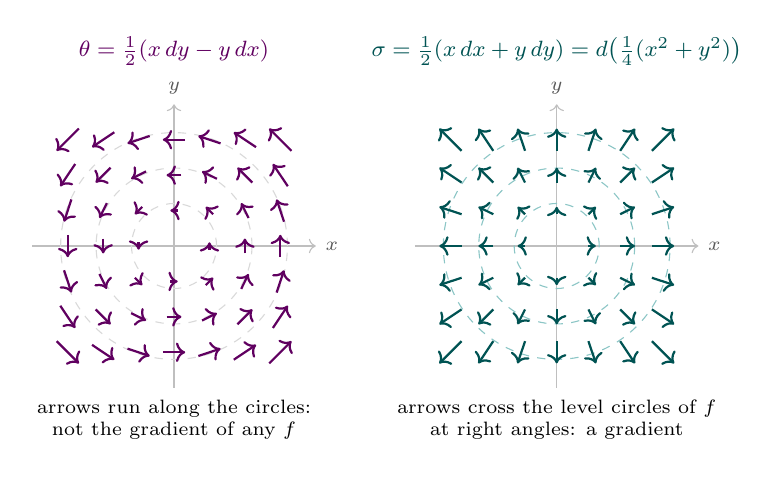
\begin{tikzpicture}[scale=0.9]
\draw[->, gray!50] (-2.00,0) -- (2.00,0) node[right, font=\scriptsize, text=gray!70!black] {$x$};
\draw[->, gray!50] (0.00,-2.0) -- (0.00,2.0) node[above, font=\scriptsize, text=gray!70!black] {$y$};
\draw[gray!30, dashed] (0.00,0) circle (0.60);
\draw[gray!30, dashed] (0.00,0) circle (1.10);
\draw[gray!30, dashed] (0.00,0) circle (1.60);
\draw[->, violet!75!black, thick] (-1.657,-1.343) -- (-1.343,-1.657);
\draw[->, violet!75!black, thick] (-1.605,-0.843) -- (-1.395,-1.157);
\draw[->, violet!75!black, thick] (-1.552,-0.343) -- (-1.448,-0.657);
\draw[->, violet!75!black, thick] (-1.500,0.158) -- (-1.500,-0.158);
\draw[->, violet!75!black, thick] (-1.448,0.657) -- (-1.552,0.343);
\draw[->, violet!75!black, thick] (-1.395,1.157) -- (-1.605,0.843);
\draw[->, violet!75!black, thick] (-1.343,1.657) -- (-1.657,1.343);
\draw[->, violet!75!black, thick] (-1.157,-1.395) -- (-0.843,-1.605);
\draw[->, violet!75!black, thick] (-1.105,-0.895) -- (-0.895,-1.105);
\draw[->, violet!75!black, thick] (-1.052,-0.395) -- (-0.948,-0.605);
\draw[->, violet!75!black, thick] (-1.000,0.105) -- (-1.000,-0.105);
\draw[->, violet!75!black, thick] (-0.948,0.605) -- (-1.052,0.395);
\draw[->, violet!75!black, thick] (-0.895,1.105) -- (-1.105,0.895);
\draw[->, violet!75!black, thick] (-0.843,1.605) -- (-1.157,1.395);
\draw[->, violet!75!black, thick] (-0.657,-1.448) -- (-0.343,-1.552);
\draw[->, violet!75!black, thick] (-0.605,-0.948) -- (-0.395,-1.052);
\draw[->, violet!75!black, thick] (-0.552,-0.448) -- (-0.448,-0.552);
\draw[->, violet!75!black, thick] (-0.500,0.052) -- (-0.500,-0.052);
\draw[->, violet!75!black, thick] (-0.448,0.552) -- (-0.552,0.448);
\draw[->, violet!75!black, thick] (-0.395,1.052) -- (-0.605,0.948);
\draw[->, violet!75!black, thick] (-0.343,1.552) -- (-0.657,1.448);
\draw[->, violet!75!black, thick] (-0.158,-1.500) -- (0.158,-1.500);
\draw[->, violet!75!black, thick] (-0.105,-1.000) -- (0.105,-1.000);
\draw[->, violet!75!black, thick] (-0.052,-0.500) -- (0.052,-0.500);
\draw[->, violet!75!black, thick] (0.052,0.500) -- (-0.052,0.500);
\draw[->, violet!75!black, thick] (0.105,1.000) -- (-0.105,1.000);
\draw[->, violet!75!black, thick] (0.158,1.500) -- (-0.158,1.500);
\draw[->, violet!75!black, thick] (0.343,-1.552) -- (0.657,-1.448);
\draw[->, violet!75!black, thick] (0.395,-1.052) -- (0.605,-0.948);
\draw[->, violet!75!black, thick] (0.448,-0.552) -- (0.552,-0.448);
\draw[->, violet!75!black, thick] (0.500,-0.052) -- (0.500,0.052);
\draw[->, violet!75!black, thick] (0.552,0.448) -- (0.448,0.552);
\draw[->, violet!75!black, thick] (0.605,0.948) -- (0.395,1.052);
\draw[->, violet!75!black, thick] (0.657,1.448) -- (0.343,1.552);
\draw[->, violet!75!black, thick] (0.843,-1.605) -- (1.157,-1.395);
\draw[->, violet!75!black, thick] (0.895,-1.105) -- (1.105,-0.895);
\draw[->, violet!75!black, thick] (0.948,-0.605) -- (1.052,-0.395);
\draw[->, violet!75!black, thick] (1.000,-0.105) -- (1.000,0.105);
\draw[->, violet!75!black, thick] (1.052,0.395) -- (0.948,0.605);
\draw[->, violet!75!black, thick] (1.105,0.895) -- (0.895,1.105);
\draw[->, violet!75!black, thick] (1.157,1.395) -- (0.843,1.605);
\draw[->, violet!75!black, thick] (1.343,-1.657) -- (1.657,-1.343);
\draw[->, violet!75!black, thick] (1.395,-1.157) -- (1.605,-0.843);
\draw[->, violet!75!black, thick] (1.448,-0.657) -- (1.552,-0.343);
\draw[->, violet!75!black, thick] (1.500,-0.158) -- (1.500,0.158);
\draw[->, violet!75!black, thick] (1.552,0.343) -- (1.448,0.657);
\draw[->, violet!75!black, thick] (1.605,0.843) -- (1.395,1.157);
\draw[->, violet!75!black, thick] (1.657,1.343) -- (1.343,1.657);
\draw[->, gray!50] (3.40,0) -- (7.40,0) node[right, font=\scriptsize, text=gray!70!black] {$x$};
\draw[->, gray!50] (5.40,-2.0) -- (5.40,2.0) node[above, font=\scriptsize, text=gray!70!black] {$y$};
\draw[teal!45, dashed] (5.40,0) circle (0.60);
\draw[teal!45, dashed] (5.40,0) circle (1.10);
\draw[teal!45, dashed] (5.40,0) circle (1.60);
\draw[->, teal!65!black, thick] (4.058,-1.343) -- (3.743,-1.657);
\draw[->, teal!65!black, thick] (4.058,-0.895) -- (3.743,-1.105);
\draw[->, teal!65!black, thick] (4.058,-0.448) -- (3.743,-0.552);
\draw[->, teal!65!black, thick] (4.058,0.000) -- (3.743,0.000);
\draw[->, teal!65!black, thick] (4.058,0.448) -- (3.743,0.552);
\draw[->, teal!65!black, thick] (4.058,0.895) -- (3.743,1.105);
\draw[->, teal!65!black, thick] (4.058,1.343) -- (3.743,1.657);
\draw[->, teal!65!black, thick] (4.505,-1.343) -- (4.295,-1.657);
\draw[->, teal!65!black, thick] (4.505,-0.895) -- (4.295,-1.105);
\draw[->, teal!65!black, thick] (4.505,-0.448) -- (4.295,-0.552);
\draw[->, teal!65!black, thick] (4.505,0.000) -- (4.295,0.000);
\draw[->, teal!65!black, thick] (4.505,0.448) -- (4.295,0.552);
\draw[->, teal!65!black, thick] (4.505,0.895) -- (4.295,1.105);
\draw[->, teal!65!black, thick] (4.505,1.343) -- (4.295,1.657);
\draw[->, teal!65!black, thick] (4.953,-1.343) -- (4.848,-1.657);
\draw[->, teal!65!black, thick] (4.953,-0.895) -- (4.848,-1.105);
\draw[->, teal!65!black, thick] (4.953,-0.448) -- (4.848,-0.552);
\draw[->, teal!65!black, thick] (4.953,0.000) -- (4.848,0.000);
\draw[->, teal!65!black, thick] (4.953,0.448) -- (4.848,0.552);
\draw[->, teal!65!black, thick] (4.953,0.895) -- (4.848,1.105);
\draw[->, teal!65!black, thick] (4.953,1.343) -- (4.848,1.657);
\draw[->, teal!65!black, thick] (5.400,-1.343) -- (5.400,-1.657);
\draw[->, teal!65!black, thick] (5.400,-0.895) -- (5.400,-1.105);
\draw[->, teal!65!black, thick] (5.400,-0.448) -- (5.400,-0.552);
\draw[->, teal!65!black, thick] (5.400,0.448) -- (5.400,0.552);
\draw[->, teal!65!black, thick] (5.400,0.895) -- (5.400,1.105);
\draw[->, teal!65!black, thick] (5.400,1.343) -- (5.400,1.657);
\draw[->, teal!65!black, thick] (5.848,-1.343) -- (5.953,-1.657);
\draw[->, teal!65!black, thick] (5.848,-0.895) -- (5.953,-1.105);
\draw[->, teal!65!black, thick] (5.848,-0.448) -- (5.953,-0.552);
\draw[->, teal!65!black, thick] (5.848,0.000) -- (5.953,0.000);
\draw[->, teal!65!black, thick] (5.848,0.448) -- (5.953,0.552);
\draw[->, teal!65!black, thick] (5.848,0.895) -- (5.953,1.105);
\draw[->, teal!65!black, thick] (5.848,1.343) -- (5.953,1.657);
\draw[->, teal!65!black, thick] (6.295,-1.343) -- (6.505,-1.657);
\draw[->, teal!65!black, thick] (6.295,-0.895) -- (6.505,-1.105);
\draw[->, teal!65!black, thick] (6.295,-0.448) -- (6.505,-0.552);
\draw[->, teal!65!black, thick] (6.295,0.000) -- (6.505,0.000);
\draw[->, teal!65!black, thick] (6.295,0.448) -- (6.505,0.552);
\draw[->, teal!65!black, thick] (6.295,0.895) -- (6.505,1.105);
\draw[->, teal!65!black, thick] (6.295,1.343) -- (6.505,1.657);
\draw[->, teal!65!black, thick] (6.743,-1.343) -- (7.058,-1.657);
\draw[->, teal!65!black, thick] (6.743,-0.895) -- (7.058,-1.105);
\draw[->, teal!65!black, thick] (6.743,-0.448) -- (7.058,-0.552);
\draw[->, teal!65!black, thick] (6.743,0.000) -- (7.058,0.000);
\draw[->, teal!65!black, thick] (6.743,0.448) -- (7.058,0.552);
\draw[->, teal!65!black, thick] (6.743,0.895) -- (7.058,1.105);
\draw[->, teal!65!black, thick] (6.743,1.343) -- (7.058,1.657);
\node[font=\footnotesize, violet!75!black] at (0,2.75) {$\theta = \tfrac12(x\,dy - y\,dx)$};
\node[font=\footnotesize, teal!65!black] at (5.4,2.75) {$\sigma = \tfrac12(x\,dx + y\,dy) = d\big(\tfrac14(x^2+y^2)\big)$};
\node[font=\scriptsize, align=center] at (0,-2.45) {arrows run along the circles:\\ not the gradient of any $f$};
\node[font=\scriptsize, align=center] at (5.4,-2.45) {arrows cross the level circles of $f$\\ at right angles: a gradient};
\end{tikzpicture}
\end{center}

The two forms of Example~\ref{ex:two-one-forms}, drawn as arrows. A one-form is not an arrow --- it eats arrows --- so the picture uses the Euclidean dot product to turn $a\,dx + b\,dy$ into the vector $(a, b)$; this identification is available in $\mathbb{R}^2$, not on a general manifold, and it is how ``$df$'' becomes the ``gradient'' of calculus. Right: $\sigma = df$ for $f = \tfrac14(x^2+y^2)$, and its arrows cross the level circles of $f$ at right angles, as a gradient's must. Left: $\theta$'s arrows run \emph{along} the circles. If $\theta$ were $df$, then $f$ would increase steadily all the way around a circle and return to its starting value --- impossible.

\begin{rembox}[The Condition Is Not Sufficient]\label{rem:condition-not-sufficient}
The mixed-partials condition is necessary but not sufficient, and Uribe flagged this as ``the beginning of de Rham theory'': whether it suffices ``has to do with the topology of the domain.'' The standard example (Lee, Example~11.36; not from lecture) is
\[
\omega = \frac{x\, dy - y\, dx}{x^2 + y^2} \quad \text{on } \mathbb{R}^2 \setminus \{0\} .
\]
It satisfies the condition: both mixed partials equal $(y^2 - x^2)/(x^2 + y^2)^2$. But it is not $df$. Along the circle $c(t) = (\cos t, \sin t)$, with velocity $c'(t) = -\sin t\, \partial_x + \cos t\, \partial_y$ (\ref{sec:velocities}), one finds $\omega(c'(t)) = 1$. If $\omega = df$, then $(f \circ c)'(t) = df(c'(t)) = 1$, so $f(c(2\pi)) - f(c(0)) = 2\pi$; but $c(2\pi) = c(0)$. The hole at the origin is what makes this possible: on all of $\mathbb{R}^2$ --- indeed on any star-shaped domain --- the condition is sufficient (Lee, Corollary~11.50).
\end{rembox}

\subsection{Pullbacks of One-Forms}\label{sub:pullback-one-forms}

\begin{defbox}[Pullback of One-Forms]\deflabel{def:pullback-one-form}
Let $F : M \to N$ be smooth. The \textbf{pullback} of functions is $F^*f = f \circ F$. For a one-form $\theta$ on $N$, the \textbf{pullback} $F^*\theta$ is the section of $T^*M$ whose value at $p$ is the pullback of the covector $\theta_{F(p)}$ (Definition~\ref{def:pullback-covector}):
\[
(F^*\theta)_p = F_p^*\big(\theta_{F(p)}\big), \qquad (F^*\theta)_p(v) = \theta_{F(p)}\big(F_{*p}v\big) .
\]
It is smooth, hence a one-form, by Proposition~\ref{prop:pullback-coords} below.
\leeref{Ch.~11, \emph{Pullbacks of Covector Fields}}
\end{defbox}

\begin{corbox}[Pullback Commutes with $d$]\thmlabel{cor:pullback-d-forms}
Let $F : M \to N$ be smooth and $f \in C^\infty(N)$. Then $F^*(df) = d(F^*f)$ as one-forms on $M$.
\leeref{Proposition 11.25}
\end{corbox}

\begin{proof}
\textit{(Lecture~15 stated it in this form, ``one says that the pullback map commutes with $d$''.)} At each $p \in M$ the two sides are $F_p^*(df_{F(p)})$ and $d(f \circ F)_p$, which agree by Proposition~\ref{prop:pullback-d}.
\end{proof}

\begin{propbox}[Pullbacks in Coordinates]\thmlabel{prop:pullback-coords}
In charts $(x^i)$ on $M$ and $(y^j)$ on $N$, with $F^j = y^j \circ F$,
\[
F^*\Big(\sum_j \theta_j\, dy^j\Big) = \sum_i \Big( \sum_j (\theta_j \circ F)\, \frac{\partial F^j}{\partial x^i} \Big)\, dx^i .
\]
In particular $F^*\theta$ is smooth whenever $\theta$ is.
\end{propbox}

\begin{proof}
\textit{(Not from lecture; filled in.)} Evaluate both sides on $\partial/\partial x^i|_p$: by definition the left side gives $\sum_j \theta_j(F(p))\, dy^j|_{F(p)}\big(F_{*p}\, \partial/\partial x^i|_p\big)$, and $F_{*p}\, \partial/\partial x^i|_p = \sum_j \partial F^j/\partial x^i(p)\, \partial/\partial y^j|_{F(p)}$ (Theorem~\ref{lem:differential-matrix}). Smoothness follows from Proposition~\ref{prop:one-form-coords}.
\end{proof}

% ============================================================================
% SECTION: VECTOR FIELDS
% ============================================================================

\section{Vector Fields}\label{sec:fields}\label{sub:sections}\label{sub:vector-fields}\label{sec:vf-operators}

\roadmark{Stage: fields}{Smooth sections of $TM$, a tangent vector at every point --- and vector fields acting on functions, as derivations of $C^\infty(M)$.}

\textit{Lecture 15: ``now we want to start a big chapter, new chapter, and now it is on vector fields.'' References: Lee Ch.~8.} The definition itself was given in Lectures~12 and~13, with the tangent bundle; Lecture~15 restated it ``analogously'' to one-forms.

\subsection{Vector Fields and Their Coordinates}\label{sub:vf-def}

\begin{defbox}[Vector Field]\deflabel{def:vector-field}
A \textbf{vector field} on $M$ is a section of the tangent bundle $\pi : TM \to M$: a smooth map $\mathbf{X} : M \to TM$ with $\mathbf{X}(p) \in T_pM$ for every $p$ --- ``for every point, [it] selects a tangent vector at that point.''
\leeref{Ch.~8, \emph{Vector Fields}}
\end{defbox}

\textbf{Transcription note.} Page~36 of the handwritten notes writes ``Section of $TM \xrightarrow{F} M$''; the map is the projection $\pi$.

\begin{defbox}[The Space of Vector Fields]\deflabel{def:vector-fields-space}
A vector field on $M$ is a smooth section $\mathbf{X}$ of the tangent bundle $TM \to M$ (Definition~\ref{def:vector-field}); its value at $p$ is written $\mathbf{X}_p \in T_pM$, again with $p$ as a subscript, to make room for the function a tangent vector acts on. The set of all vector fields on $M$ is denoted
\[
\mathfrak{X}(M) \qquad \text{(\LaTeX: \texttt{\textbackslash mathfrak\{X\}})}.
\]
It is a real vector space, and functions multiply vector fields pointwise: $(f\mathbf{X})_p = f(p) \mathbf{X}_p$.
\leeref{Ch.~8, \emph{Vector Fields on Manifolds}}
\end{defbox}

\begin{propbox}[Vector Fields in Coordinates]\thmlabel{prop:vf-coords}
Let $\mathbf{X}$ be a section of $TM$ (not assumed smooth) and $(U, \varphi = (x^j))$ a chart. Then on $U$
\[
\mathbf{X} = \sum_{j=1}^m \mathbf{X}^j\, \frac{\partial}{\partial x^j}, \qquad \mathbf{X}^j(p) = \mathbf{X}_p[x^j] = dx^j|_p(\mathbf{X}_p),
\]
and $\mathbf{X}$ is smooth on $U$ if and only if the coefficient functions $\mathbf{X}^1, \ldots, \mathbf{X}^m$ are smooth on $U$.
\leeref{Proposition 8.1}
\end{propbox}

\begin{proof}
\textit{(Stated in Lecture~15, ``analogously'' to one-forms; filled in.)} The expansion is the basis theorem at each point, with coefficients $\mathbf{X}_p[x^j]$ (Theorem~\ref{thm:tangent-basis}). In the chart $\tilde\varphi$ of $TM$ (Definition~\ref{def:tb-chart}) the coordinate representation of $\mathbf{X}$ is $r \mapsto \big(r, \mathbf{X}^1(\varphi^{-1}(r)), \ldots, \mathbf{X}^m(\varphi^{-1}(r))\big)$, smooth exactly when every $\mathbf{X}^j \circ \varphi^{-1}$ is.
\end{proof}

\begin{rembox}[Vector Fields and One-Forms Side by Side]\label{rem:fields-side-by-side}
\begin{center}
\renewcommand{\arraystretch}{1.3}
\begin{tabular}{p{0.2\textwidth} p{0.26\textwidth} p{0.2\textwidth} p{0.22\textwidth}}
\hline
Field & A section of & In a chart & Picture \\
\hline
vector field $\mathbf{X}$ & $TM$ (Definition~\ref{def:vector-field}) & $\sum_j \mathbf{X}^j\, \partial/\partial x^j$ & wind on the surface \\
one-form $\theta$ & $T^*M$ (Definition~\ref{def:one-form}) & $\sum_j \theta_j\, dx^j$ & a rule pricing every step \\
\hline
\end{tabular}
\end{center}
Every function gives a one-form, $f \mapsto df$ (Proposition~\ref{prop:d-operator}), but not every one-form is a $df$ (Proposition~\ref{prop:exactness-test}). A one-form and a vector field together give a function, $p \mapsto \theta_p(\mathbf{X}_p)$. And a vector field acting on a function gives a function, $p \mapsto \mathbf{X}_p[f]$ --- the starting point of the next subsection.
\end{rembox}

\subsection{Vector Fields as Derivations}\label{sub:vf-derivations}

\begin{rembox}[Two Faces of a Vector Field]\label{rem:two-faces-vector-field}
``Just as tangent vectors, fields have a double life.'' Tangent vectors were defined as derivations and then shown to be velocities of curves (\ref{sec:velocities}). Vector fields likewise have two faces: \emph{operators on functions}, studied first because it continues the definition by derivations; and \emph{dynamics on $M$} --- integral curves, the trajectories that follow the field, to come later.
\end{rembox}

\begin{defbox}[Derivation of $C^\infty(M)$]\deflabel{def:global-derivation}
A \textbf{derivation} of $C^\infty(M)$ is an $\mathbb{R}$-linear map $D : C^\infty(M) \to C^\infty(M)$ satisfying the product rule
\[
D(fg) = f\, Dg + g\, Df \qquad \text{for all } f, g \in C^\infty(M).
\]
Compare a derivation \emph{at a point} (Definition~\ref{def:derivation}), which takes values in $\mathbb{R}$ and acts on germs.
\leeref{Ch.~8, \emph{Vector Fields as Derivations}}
\end{defbox}

\begin{lembox}[A Vector Field Is a Derivation]\thmlabel{lem:vf-derivation}
For $\mathbf{X} \in \mathfrak{X}(M)$ and $f \in C^\infty(M)$, the function $D_\mathbf{X}f : p \mapsto \mathbf{X}_p[f]$ is smooth, and $D_\mathbf{X} : C^\infty(M) \to C^\infty(M)$ is a derivation. In a chart, $D_\mathbf{X}f = \sum_j \mathbf{X}^j\, \partial f/\partial x^j$. (Lee writes $\mathbf{X}f$ for $D_\mathbf{X}f$.)
\end{lembox}

\begin{proof}
\textit{(Lecture~15: linearity and the product rule are ``an immediate consequence of the corresponding properties for tangent vectors'', applied at each point. Smoothness of $D_\mathbf{X}f$, which the lecture did not address, is filled in.)} In a chart, $\mathbf{X}_p[f] = \sum_j \mathbf{X}^j(p)\, \partial f/\partial x^j(p)$ by Proposition~\ref{prop:vf-coords}, a sum of products of smooth functions. At each $p$, $\mathbf{X}_p[fg] = f(p)\, \mathbf{X}_p[g] + g(p)\, \mathbf{X}_p[f]$ because $\mathbf{X}_p$ is a derivation at $p$; that is the product rule for $D_\mathbf{X}$, and linearity is the same.
\end{proof}

The goal of this section is the converse of the lemma: every derivation of $C^\infty(M)$ comes from a vector field (Proposition~\ref{prop:derivations-are-fields}, at the end). Tangent vectors act on germs, which only see a neighbourhood of a point, while a derivation of $C^\infty(M)$ acts on functions on all of $M$. The bridge is locality (Lemma~\ref{lem:derivation-local}), and its proof needs bump functions, so these come first.

\begin{defbox}[Local Operator]\deflabel{def:local-operator}
An operator $D : C^\infty(M) \to C^\infty(M)$ is \textbf{local} if for every open $U \subseteq M$ and all $f, g \in C^\infty(M)$,
\[
f|_U = g|_U \quad \Longrightarrow \quad (Df)|_U = (Dg)|_U .
\]
\end{defbox}

``Even though $D$ a priori is defined on functions on $M$, it's actually going to be given by local data'': knowing $f$ on $U$ determines $Df$ on $U$.

\begin{defbox}[Support]\deflabel{def:support}
The \textbf{support} of a function $\chi : M \to \mathbb{R}$ is the \emph{closure} of the set where it is nonzero,
\[
\operatorname{supp}\chi = \overline{\{ q \in M : \chi(q) \neq 0 \}} ,
\]
and $C^\infty_0(M)$ is the set of smooth functions with compact support.
\leeref{Ch.~2, \emph{Partitions of Unity}}
\end{defbox}

\begin{defbox}[Bump Function]\deflabel{def:bump-function}
Let $p \in M$. A \textbf{bump function at $p$} is a $\chi \in C^\infty_0(M)$ (Definition~\ref{def:support}) with $\chi \equiv 1$ on a neighbourhood of $p$.
\leeref{Ch.~2, \emph{Partitions of Unity}}
\end{defbox}

``It's a technical term, and it's not a joke'': the graph is a plateau, equal to $1$ near $p$ and dying off to $0$ outside a compact set --- ``smooth, but not analytic'', since an analytic function equal to $1$ on an open set would equal $1$ on the whole connected domain.

\begin{center}
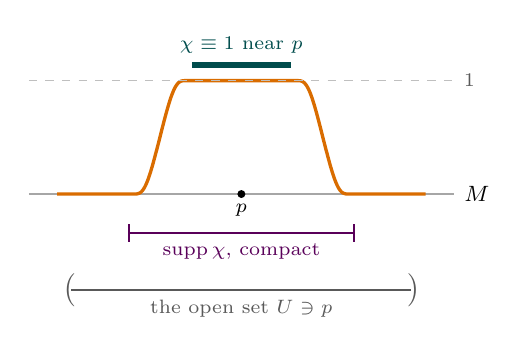
\begin{tikzpicture}[scale=0.9]
\draw[thick, gray!70] (-3.0,0) -- (3.0,0) node[right, font=\footnotesize, text=black] {$M$};
\draw[orange!85!black, very thick] (-2.600,0.000) -- (-2.587,0.000) -- (-2.574,0.000) -- (-2.561,0.000) -- (-2.548,0.000) -- (-2.535,0.000) -- (-2.522,0.000) -- (-2.509,0.000) -- (-2.496,0.000) -- (-2.483,0.000) -- (-2.470,0.000) -- (-2.457,0.000) -- (-2.444,0.000) -- (-2.431,0.000) -- (-2.418,0.000) -- (-2.405,0.000) -- (-2.391,0.000) -- (-2.378,0.000) -- (-2.365,0.000) -- (-2.352,0.000) -- (-2.339,0.000) -- (-2.326,0.000) -- (-2.313,0.000) -- (-2.300,0.000) -- (-2.287,0.000) -- (-2.274,0.000) -- (-2.261,0.000) -- (-2.248,0.000) -- (-2.235,0.000) -- (-2.222,0.000) -- (-2.209,0.000) -- (-2.196,0.000) -- (-2.183,0.000) -- (-2.170,0.000) -- (-2.157,0.000) -- (-2.144,0.000) -- (-2.131,0.000) -- (-2.118,0.000) -- (-2.105,0.000) -- (-2.092,0.000) -- (-2.079,0.000) -- (-2.066,0.000) -- (-2.053,0.000) -- (-2.040,0.000) -- (-2.027,0.000) -- (-2.014,0.000) -- (-2.001,0.000) -- (-1.987,0.000) -- (-1.974,0.000) -- (-1.961,0.000) -- (-1.948,0.000) -- (-1.935,0.000) -- (-1.922,0.000) -- (-1.909,0.000) -- (-1.896,0.000) -- (-1.883,0.000) -- (-1.870,0.000) -- (-1.857,0.000) -- (-1.844,0.000) -- (-1.831,0.000) -- (-1.818,0.000) -- (-1.805,0.000) -- (-1.792,0.000) -- (-1.779,0.000) -- (-1.766,0.000) -- (-1.753,0.000) -- (-1.740,0.000) -- (-1.727,0.000) -- (-1.714,0.000) -- (-1.701,0.000) -- (-1.688,0.000) -- (-1.675,0.000) -- (-1.662,0.000) -- (-1.649,0.000) -- (-1.636,0.000) -- (-1.623,0.000) -- (-1.610,0.000) -- (-1.596,0.000) -- (-1.583,0.000) -- (-1.570,0.000) -- (-1.557,0.000) -- (-1.544,0.000) -- (-1.531,0.000) -- (-1.518,0.000) -- (-1.505,0.000) -- (-1.492,0.001) -- (-1.479,0.001) -- (-1.466,0.003) -- (-1.453,0.007) -- (-1.440,0.012) -- (-1.427,0.019) -- (-1.414,0.029) -- (-1.401,0.043) -- (-1.388,0.059) -- (-1.375,0.079) -- (-1.362,0.102) -- (-1.349,0.128) -- (-1.336,0.158) -- (-1.323,0.190) -- (-1.310,0.226) -- (-1.297,0.264) -- (-1.284,0.304) -- (-1.271,0.347) -- (-1.258,0.391) -- (-1.245,0.437) -- (-1.232,0.485) -- (-1.219,0.533) -- (-1.206,0.583) -- (-1.192,0.633) -- (-1.179,0.684) -- (-1.166,0.735) -- (-1.153,0.787) -- (-1.140,0.838) -- (-1.127,0.889) -- (-1.114,0.941) -- (-1.101,0.991) -- (-1.088,1.041) -- (-1.075,1.090) -- (-1.062,1.138) -- (-1.049,1.185) -- (-1.036,1.230) -- (-1.023,1.274) -- (-1.010,1.315) -- (-0.997,1.355) -- (-0.984,1.392) -- (-0.971,1.426) -- (-0.958,1.457) -- (-0.945,1.485) -- (-0.932,1.510) -- (-0.919,1.531) -- (-0.906,1.549) -- (-0.893,1.564) -- (-0.880,1.576) -- (-0.867,1.585) -- (-0.854,1.591) -- (-0.841,1.595) -- (-0.828,1.598) -- (-0.815,1.599) -- (-0.802,1.600) -- (-0.788,1.600) -- (-0.775,1.600) -- (-0.762,1.600) -- (-0.749,1.600) -- (-0.736,1.600) -- (-0.723,1.600) -- (-0.710,1.600) -- (-0.697,1.600) -- (-0.684,1.600) -- (-0.671,1.600) -- (-0.658,1.600) -- (-0.645,1.600) -- (-0.632,1.600) -- (-0.619,1.600) -- (-0.606,1.600) -- (-0.593,1.600) -- (-0.580,1.600) -- (-0.567,1.600) -- (-0.554,1.600) -- (-0.541,1.600) -- (-0.528,1.600) -- (-0.515,1.600) -- (-0.502,1.600) -- (-0.489,1.600) -- (-0.476,1.600) -- (-0.463,1.600) -- (-0.450,1.600) -- (-0.437,1.600) -- (-0.424,1.600) -- (-0.411,1.600) -- (-0.397,1.600) -- (-0.384,1.600) -- (-0.371,1.600) -- (-0.358,1.600) -- (-0.345,1.600) -- (-0.332,1.600) -- (-0.319,1.600) -- (-0.306,1.600) -- (-0.293,1.600) -- (-0.280,1.600) -- (-0.267,1.600) -- (-0.254,1.600) -- (-0.241,1.600) -- (-0.228,1.600) -- (-0.215,1.600) -- (-0.202,1.600) -- (-0.189,1.600) -- (-0.176,1.600) -- (-0.163,1.600) -- (-0.150,1.600) -- (-0.137,1.600) -- (-0.124,1.600) -- (-0.111,1.600) -- (-0.098,1.600) -- (-0.085,1.600) -- (-0.072,1.600) -- (-0.059,1.600) -- (-0.046,1.600) -- (-0.033,1.600) -- (-0.020,1.600) -- (-0.007,1.600) -- (0.007,1.600) -- (0.020,1.600) -- (0.033,1.600) -- (0.046,1.600) -- (0.059,1.600) -- (0.072,1.600) -- (0.085,1.600) -- (0.098,1.600) -- (0.111,1.600) -- (0.124,1.600) -- (0.137,1.600) -- (0.150,1.600) -- (0.163,1.600) -- (0.176,1.600) -- (0.189,1.600) -- (0.202,1.600) -- (0.215,1.600) -- (0.228,1.600) -- (0.241,1.600) -- (0.254,1.600) -- (0.267,1.600) -- (0.280,1.600) -- (0.293,1.600) -- (0.306,1.600) -- (0.319,1.600) -- (0.332,1.600) -- (0.345,1.600) -- (0.358,1.600) -- (0.371,1.600) -- (0.384,1.600) -- (0.397,1.600) -- (0.411,1.600) -- (0.424,1.600) -- (0.437,1.600) -- (0.450,1.600) -- (0.463,1.600) -- (0.476,1.600) -- (0.489,1.600) -- (0.502,1.600) -- (0.515,1.600) -- (0.528,1.600) -- (0.541,1.600) -- (0.554,1.600) -- (0.567,1.600) -- (0.580,1.600) -- (0.593,1.600) -- (0.606,1.600) -- (0.619,1.600) -- (0.632,1.600) -- (0.645,1.600) -- (0.658,1.600) -- (0.671,1.600) -- (0.684,1.600) -- (0.697,1.600) -- (0.710,1.600) -- (0.723,1.600) -- (0.736,1.600) -- (0.749,1.600) -- (0.762,1.600) -- (0.775,1.600) -- (0.788,1.600) -- (0.802,1.600) -- (0.815,1.599) -- (0.828,1.598) -- (0.841,1.595) -- (0.854,1.591) -- (0.867,1.585) -- (0.880,1.576) -- (0.893,1.564) -- (0.906,1.549) -- (0.919,1.531) -- (0.932,1.510) -- (0.945,1.485) -- (0.958,1.457) -- (0.971,1.426) -- (0.984,1.392) -- (0.997,1.355) -- (1.010,1.315) -- (1.023,1.274) -- (1.036,1.230) -- (1.049,1.185) -- (1.062,1.138) -- (1.075,1.090) -- (1.088,1.041) -- (1.101,0.991) -- (1.114,0.941) -- (1.127,0.889) -- (1.140,0.838) -- (1.153,0.787) -- (1.166,0.735) -- (1.179,0.684) -- (1.192,0.633) -- (1.206,0.583) -- (1.219,0.533) -- (1.232,0.485) -- (1.245,0.437) -- (1.258,0.391) -- (1.271,0.347) -- (1.284,0.304) -- (1.297,0.264) -- (1.310,0.226) -- (1.323,0.190) -- (1.336,0.158) -- (1.349,0.128) -- (1.362,0.102) -- (1.375,0.079) -- (1.388,0.059) -- (1.401,0.043) -- (1.414,0.029) -- (1.427,0.019) -- (1.440,0.012) -- (1.453,0.007) -- (1.466,0.003) -- (1.479,0.001) -- (1.492,0.001) -- (1.505,0.000) -- (1.518,0.000) -- (1.531,0.000) -- (1.544,0.000) -- (1.557,0.000) -- (1.570,0.000) -- (1.583,0.000) -- (1.596,0.000) -- (1.610,0.000) -- (1.623,0.000) -- (1.636,0.000) -- (1.649,0.000) -- (1.662,0.000) -- (1.675,0.000) -- (1.688,0.000) -- (1.701,0.000) -- (1.714,0.000) -- (1.727,0.000) -- (1.740,0.000) -- (1.753,0.000) -- (1.766,0.000) -- (1.779,0.000) -- (1.792,0.000) -- (1.805,0.000) -- (1.818,0.000) -- (1.831,0.000) -- (1.844,0.000) -- (1.857,0.000) -- (1.870,0.000) -- (1.883,0.000) -- (1.896,0.000) -- (1.909,0.000) -- (1.922,0.000) -- (1.935,0.000) -- (1.948,0.000) -- (1.961,0.000) -- (1.974,0.000) -- (1.987,0.000) -- (2.001,0.000) -- (2.014,0.000) -- (2.027,0.000) -- (2.040,0.000) -- (2.053,0.000) -- (2.066,0.000) -- (2.079,0.000) -- (2.092,0.000) -- (2.105,0.000) -- (2.118,0.000) -- (2.131,0.000) -- (2.144,0.000) -- (2.157,0.000) -- (2.170,0.000) -- (2.183,0.000) -- (2.196,0.000) -- (2.209,0.000) -- (2.222,0.000) -- (2.235,0.000) -- (2.248,0.000) -- (2.261,0.000) -- (2.274,0.000) -- (2.287,0.000) -- (2.300,0.000) -- (2.313,0.000) -- (2.326,0.000) -- (2.339,0.000) -- (2.352,0.000) -- (2.365,0.000) -- (2.378,0.000) -- (2.391,0.000) -- (2.405,0.000) -- (2.418,0.000) -- (2.431,0.000) -- (2.444,0.000) -- (2.457,0.000) -- (2.470,0.000) -- (2.483,0.000) -- (2.496,0.000) -- (2.509,0.000) -- (2.522,0.000) -- (2.535,0.000) -- (2.548,0.000) -- (2.561,0.000) -- (2.574,0.000) -- (2.587,0.000) -- (2.600,0.000);
\draw[gray!50, dashed] (-3.0,1.60) -- (3.0,1.60) node[right, font=\scriptsize, text=gray!70!black] {$1$};
\fill (0,0) circle (1.6pt) node[below, font=\scriptsize] {$p$};
\draw[teal!60!black, line width=2.2pt] (-0.70,1.82) -- (0.70,1.82);
\node[teal!60!black, font=\scriptsize, above] at (0,1.85) {$\chi \equiv 1$ near $p$};
\draw[violet!70!black, |-|, thick] (-1.60,-0.55) -- node[below, font=\scriptsize] {$\operatorname{supp}\chi$, compact} (1.60,-0.55);
\draw[gray!70!black, thick] (-2.4,-1.35) -- node[below, font=\scriptsize] {the open set $U \ni p$} (2.4,-1.35); \node[gray!70!black, font=\large] at (-2.42,-1.35) {(}; \node[gray!70!black, font=\large] at (2.42,-1.35) {)};
\end{tikzpicture}
\end{center}

A bump function, drawn over a one-dimensional slice of $M$ (the graph is the plateau of Uribe's picture, in cross-section). It equals $1$ on a neighbourhood of $p$, is smooth everywhere, and vanishes outside its support, which is compact and lies inside the given open set $U$. This one is built from $h(t) = e^{-1/t}$ for $t > 0$, $h(t) = 0$ for $t \le 0$, as $\chi(x) = h(b - |x|)/\big(h(b - |x|) + h(|x| - a)\big)$, which is $1$ for $|x| \le a$ and $0$ for $|x| \ge b$.

\textbf{Transcription note.} Page~41 of the handwritten notes defines $\operatorname{supp}(\chi) = \{q \in M : \chi(q) \neq 0\}$; the support is the \emph{closure} of that set, as Uribe said (``and then you take the closure of that''). Without the closure, the support of a bump function would not be compact.

\begin{propbox}[Bump Functions Exist]\thmlabel{prop:bump-existence}
For every open $U \subseteq M$ and every $p \in U$ there is a bump function $\chi$ at $p$ with $\operatorname{supp}\chi \subseteq U$.
\leeref{Proposition 2.25}
\end{propbox}

\begin{proof}[Proof (to be filled)]
Stated in Lecture~15, to be proved next week --- ``the week before the exam'', so Uribe will prove ``technical things that you will not be using in homework.'' ``The existence is not so obvious, but it's true.''
\end{proof}

\begin{lembox}[Derivations Are Local]\thmlabel{lem:derivation-local}
Every derivation of $C^\infty(M)$ is a local operator.
\end{lembox}

\begin{proof}[Proof (to be filled)]
Stated in Lecture~15; the proof ``uses the existence of bump functions'' (Proposition~\ref{prop:bump-existence}, above) and is to come.
\end{proof}

\begin{rembox}[Differential Operators]\label{rem:differential-operators}
The operators $D_\mathbf{X}$, $\mathbf{X} \in \mathfrak{X}(M)$, together with the multiplication operators $f \mapsto gf$, generate under composition and sums the ring of \emph{differential operators} on $M$; all of them are local. Uribe stated the converse ``FYI'', without proof: every linear local operator is a differential operator. This is Peetre's theorem; its precise form says that a linear local operator is, near each point, a differential operator of finite order --- on a non-compact $M$ the order need not be bounded globally. Stated, not proved, here.
\end{rembox}

\begin{propbox}[Derivations Are Vector Fields]\thmlabel{prop:derivations-are-fields}
Conversely, every derivation $D$ of $C^\infty(M)$ is of the form $D = D_\mathbf{X}$ for a unique $\mathbf{X} \in \mathfrak{X}(M)$.
\leeref{Proposition 8.15}
\end{propbox}

\begin{proof}[Proof (to be filled)]
Stated in Lecture~15 as ``the goal''; the proof is to come. ``It's not an immediate thing at all \ldots\ tangent vectors are defined in terms of germs'', local objects near a point, ``whereas'' a derivation of $C^\infty(M)$ ``a priori'' acts on functions on all of $M$. Locality (Lemma~\ref{lem:derivation-local}) bridges the two.
\end{proof}

\appendix
\chapter{Concordance with Lee}\label{app:lee}

These notes follow the course, and Lee's \emph{Introduction to Smooth Manifolds} (2nd ed.) is the course text. The two cover the same mathematics by different routes. The course is more algebraic --- germs, derivations of germs, the ideal $I_p$ --- and it builds tangent spaces from the geometric picture towards the abstract one, where Lee starts abstract. This appendix is for reading the two side by side. It records where the notation differs, where the routes diverge, which parts of Lee each section corresponds to, and, for every result of Lee's cited in these notes, where its counterpart is. Throughout the notes, the line \textsc{Lee}: at the foot of a box gives the same information locally.

\section*{A.1\quad Notation}
\addcontentsline{toc}{section}{A.1\quad Notation}

\begin{longtable}{>{\raggedright\arraybackslash}p{4.3cm} >{\raggedright\arraybackslash}p{4.3cm} >{\raggedright\arraybackslash}p{6.2cm}}
\toprule
\textbf{These notes} & \textbf{Lee} & \textbf{Remark} \\ \midrule \endhead
$T_pM$: derivations of germs $C_p^\infty(M)$ & $T_pM$: derivations of $C^\infty(M)$ at $p$ & Isomorphic, by Proposition~\ref{prop:germ-global}; Lee's version needs bump functions. \\
$T^{\geo}_pM$, the geometric tangent space & $\mathbb{R}^n_a$ in $\mathbb{R}^n$; $T_pS \subseteq T_pM$ for embedded $S$ & Theorem~\ref{thm:ambient-abstract}; Lee, Propositions 3.2 and 5.38. \\
$F_{*p}$ & $dF_p$ & The notes keep $dF_p$ for the vector-space differential (Definition~\ref{def:vs-differential}) and $df_p$ for functions. \\
$D_\gamma$, the velocity & $\gamma'(0)$ & The notes keep $\gamma'(0)$ for the ordinary derivative of a curve in $\mathbb{R}^N$, a geometric vector (Definition~\ref{def:velocity}). \\
$D_v$, $D_v|_a$ & $D_v|_a$ & The directional derivative (Definition~\ref{def:Dv}). \\
$[f] \in C_p^\infty(M)$, germs & --- & Lee works with global functions $C^\infty(M)$ (Definition~\ref{def:germ}). \\
$f_\varphi = f \circ \varphi^{-1}$, \ $\tilde F = \psi \circ F \circ \varphi^{-1}$ & $\hat f$, \ $\widehat F$ & Coordinate representations (Definition~\ref{def:coordinate-functions}). \\
$\sum_i a^i\, \partial/\partial x^i|_p$ & $a^i\, \partial/\partial x^i|_p$ & Lee uses the Einstein summation convention; the notes always write the sum. \\
$T_p^*M$, $df_p$, $dx^i|_p$ & the same & Definition~\ref{def:cotangent}, Lemma~\ref{lem:df-coords}. \\
$I_p$, $I_p^2$, $I_p/I_p^2$, of germs & $I_p$, $I_p^2$ of global functions (Problem 11-4) & Theorem~\ref{thm:cotangent-ideal}; Lee's version needs bump functions. \\
$\Gamma = \{(x, g \cdot x)\}$, the orbit relation & $\mathcal{O} = \{(g \cdot p, p)\}$ & The same set with the factors swapped (proof of Lee, Proposition 21.4). \\
$H_{x_0}$, the isotropy group & $G_p$ & Definition~\ref{def:isotropy}. \\
$\Phi : G/H \to X$, $gH \mapsto g \cdot x_0$ & $F : G/G_p \to M$ & Theorem~\ref{thm:GH-homeo}; Lee, Theorem 21.18. \\
$\mathfrak{g} = T^{\geo}_I G$ & $\mathrm{Lie}(G) \cong T_eG$ & The notes' $\mathfrak{g}$ is the geometric tangent space at $I$; Lee defines $\mathrm{Lie}(G)$ by left-invariant vector fields (Chapter~8). \\
$\widetilde{\mathbb{R}}$: the chart $\sqrt[3]{x}$ & Example 1.23: the chart $x^3$ & Two different non-standard structures --- the transition map between them is $y \mapsto y^9$ --- both diffeomorphic to $\mathbb{R}$ (Corollary~\ref{cor:single-chart-Rn}). \\
\bottomrule
\end{longtable}

\section*{A.2\quad Where the routes diverge}
\addcontentsline{toc}{section}{A.2\quad Where the routes diverge}

Each row is expanded in a \textbf{Comparison with Lee} paragraph at the place indicated.

\begin{longtable}{>{\raggedright\arraybackslash}p{3.2cm} >{\raggedright\arraybackslash}p{5.9cm} >{\raggedright\arraybackslash}p{5.7cm}}
\toprule
\textbf{Topic} & \textbf{These notes} & \textbf{Lee} \\ \midrule \endhead
Hausdorff quotients & One criterion for all open quotients (Theorems~\ref{thm:hausdorff-criterion} and~\ref{thm:2c-quotient}), reused for orbit and coset spaces & Checked example by example (Example 1.5, Problem 1-9) \\
Regular level sets & Implicit function theorem, topological first (Theorem~\ref{thm:regular-value}), smooth afterwards (Proposition~\ref{prop:level-set-smooth}) & Example 1.32 for one function; Corollary 5.14 via the constant-rank theorem \\
Hausdorff orbit spaces & Compact group on a Hausdorff space, purely topological (Theorem~\ref{thm:orbit-T2-strong}) & Proper actions of Lie groups (Proposition 21.4, Corollary 21.6) \\
Homogeneous spaces & $G/H$ compact and $X$ Hausdorff (Theorem~\ref{thm:GH-homeo}); the hypothesis is needed (Example~\ref{ex:GH-not-homeo}) & Smooth version, no compactness (Theorem 21.18) \\
Tangent vectors & Derivations of germs; locality is built in, and no bump functions are needed & Derivations of $C^\infty(M)$; locality from bump functions (Proposition 3.8) \\
Order of ideas & Geometric first, $T^{\geo}_pM = \ker F'(p)$ (Theorem~\ref{thm:tangent-kernel}), then derivations & Derivations first; $T_pS = \ker d\Phi_p$ later (Proposition 5.38) \\
Cotangent space & The dual, and also $I_p/I_p^2$ of germs, via a non-degenerate pairing (Theorem~\ref{thm:cotangent-ideal}) & The dual in the text (Chapter~11); $I_p/I_p^2$ of global functions, via $f \mapsto df_p$, as Problem 11-4 \\
Transversality & Level sets in Euclidean space (Theorem~\ref{thm:transverse-preimage}) & Embedded submanifolds (Theorem 6.30) \\
Linear algebra & The toolkit of \ref{sec:vector-spaces}, including the pairing theorem (Theorem~\ref{thm:pairing}) & Appendix B; dual spaces in Chapter~11 \\
\bottomrule
\end{longtable}

\section*{A.3\quad Chapter map}
\addcontentsline{toc}{section}{A.3\quad Chapter map}

\begin{longtable}{>{\raggedright\arraybackslash}p{6.4cm} >{\raggedright\arraybackslash}p{8.4cm}}
\toprule
\textbf{These notes} & \textbf{Lee} \\ \midrule \endhead
\ref{sec:review}\ Point-set review & Appendix A, \emph{Topological Spaces} and \emph{Connectedness and Compactness} \\
\ref{sec:manifolds}\ Topological manifolds & Chapter 1, \emph{Topological Manifolds}; Problems 1-1 and 1-2 \\
\ref{sec:new-spaces}--\ref{sec:open-quotients}\ Subspaces, products, quotients & Appendix A, \emph{Subspaces, Products, Disjoint Unions, and Quotients}; Problem 1-9 \\
\ref{sec:rvt}\ Regular value theorem & Appendix C (Theorem C.40); Example 1.32; Corollary 5.14 \\
\ref{sec:topgroups}\ Topological and matrix groups & Chapter 7, Examples 7.27--7.30; Propositions 21.34 and 21.35; Problem 7-4 \\
\ref{sec:actions}\ Actions and orbit spaces & Chapter 7, \emph{Group Actions and Equivariant Maps}; Lemma 21.1, Proposition 21.4 \\
\ref{sec:homogeneous}\ Homogeneous spaces & Theorems 21.17--21.20; Examples 1.36 and 21.21 \\
\ref{sec:smooth-structures}\ Differentiable structures & Chapter 1, \emph{Smooth Structures}, Examples 1.22--1.34; Chapter 2 \\
\ref{sec:euclidean}\ Manifolds in Euclidean space & Example 1.32; Chapter 5 \\
\ref{sec:vector-spaces}\ Vector spaces and matrix groups & Appendix B; Chapter 11 (dual spaces); Example 1.24; Examples 7.27 and 7.29 \\
\ref{sec:tangent}\ The geometric tangent space & Propositions 3.2, 5.37 and 5.38; Theorem 6.30 \\
\ref{sec:abstract-tangent}--\ref{sec:velocities}\ Germs, derivations, the abstract tangent space & Chapter 3 throughout, including Proposition 3.14 (products) \\
\ref{sec:cotangent}\ The cotangent space & Chapter 11, \emph{Covectors}; Problem 11-4 for $I_p/I_p^2$ \\
\ref{sec:special-maps}--\ref{sec:submersions}\ Local diffeomorphisms, submersions & Chapter 4 (Propositions 4.1 and 4.28, Theorem 4.12); Theorem C.34 \\
\ref{sec:submanifolds}\ Submanifolds & Chapter 5, \emph{Embedded Submanifolds} (Theorem 5.8, Corollary 5.14, Propositions 5.35--5.38) \\
\ref{sec:fibrations}\ Fibrations & smooth fiber bundles (Chapter 10); Chapter 10 (sections); Ehresmann's theorem is not in Lee \\
\ref{sec:immersions}\ Immersions & Chapter 4, \emph{Immersions} (Theorem 4.12); Example 4.19 \\
\ref{sec:embeddings}\ Embeddings & Chapter 4, \emph{Embeddings} (Proposition 4.22, Example 4.20); Proposition 5.2; Theorem A.57; Proposition 1.12 \\
\ref{sec:double-cover}\ The double cover $\mathrm{SU}(2) \to \SO(3)$ & Problems 7-22 and 7-23 (quaternions); Examples 7.27--7.30 (matrix groups) \\
\ref{sec:recap-tangent}--\ref{sec:recap-objects}\ Recaps: tangent vectors, covectors & Chapters 3 and 11 (overview) \\
\ref{sec:tangent-bundle}\ The tangent bundle & Chapter 3, \emph{The Tangent Bundle} (Lemma 1.35, Proposition 3.18) \\
\ref{sec:cotangent-bundle}\ The cotangent bundle & Chapter 11, \emph{The Cotangent Bundle} (Proposition 11.9); Lemma 1.35 \\
\ref{sec:d-operator}\ One-forms, the operator $d$, pullbacks & Chapter 11, \emph{Covector Fields} (Propositions 11.11 and 11.25, Example 11.36, Corollary 11.50) \\
\ref{sec:fields}\ Vector fields & Chapter 8 (Propositions 8.1 and 8.15); Proposition 2.25 (bump functions) \\
\bottomrule
\end{longtable}

\section*{A.4\quad Index from Lee to these notes}
\addcontentsline{toc}{section}{A.4\quad Index from Lee to these notes}

Every numbered result of Lee's cited in these notes, in Lee's order, with the boxes that correspond to it. The table is generated from the \textsc{Lee}: lines in the boxes, so the two always agree.

{\small
\begin{longtable}{>{\raggedright\arraybackslash}p{3.6cm} >{\raggedright\arraybackslash}p{11.2cm}}
\toprule
\textbf{Lee} & \textbf{These notes} \\ \midrule \endhead
%LEE-INDEX-ROWS-BEGIN
Theorem 1.2 & Thm.~\ref{thm:inv-dim}, Cor.~\ref{cor:dim-loc-const} \\
Example 1.4 & Ex.~\ref{ex:s2-manifold}, Prop.~\ref{prop:sn-manifold}, Ex.~\ref{ex:circle-four} \\
Example 1.5 & Prop.~\ref{prop:rpn-topologies} \\
Example 1.8 & Thm.~\ref{thm:product-inherit} \\
Proposition 1.11 & Prop.~\ref{prop:count-components}, Thm.~\ref{thm:conn-implies-path}, Cor.~\ref{cor:manifold-components} \\
Proposition 1.12 & Prop.~\ref{prop:locally-compact} \\
Proposition 1.17 & Def.~\ref{def:compatible-atlases}, Thm.~\ref{thm:maximal-atlas} \\
Example 1.21 & Prop.~\ref{prop:zero-manifolds} \\
Example 1.22 & Ex.~\ref{ex:atlas-Rn} \\
Example 1.23 & Ex.~\ref{ex:two-structures-R}, Cor.~\ref{cor:single-chart-Rn}, Ex.~\ref{ex:cube-root-transport} \\
Example 1.24 & Def.~\ref{def:linear-coords}, Prop.~\ref{prop:vs-manifold}, Def.~\ref{def:vs-structure} \\
Example 1.25 & Def.~\ref{def:mat-euclid} \\
Example 1.26 & Prop.~\ref{prop:open-submanifold}, Def.~\ref{def:open-submanifold} \\
Example 1.27 & Def.~\ref{def:GL}, Prop.~\ref{prop:GL-topgroup}, Thm.~\ref{thm:classical-manifolds} \\
Example 1.31 & Ex.~\ref{ex:circle-four} \\
Example 1.32 & Thm.~\ref{thm:regular-value}, Prop.~\ref{prop:level-set-smooth} \\
Example 1.33 & Cor.~\ref{cor:rpn-atlas}, Prop.~\ref{prop:rpn-topologies} \\
Example 1.34 & Prop.~\ref{prop:product-manifold} \\
Lemma 1.35 & Prop.~\ref{prop:tb-topology}, Prop.~\ref{prop:ctb-topology} \\
Example 1.36 & Def.~\ref{def:grassmannian}, Cor.~\ref{cor:grassmannian} \\
Problem 1-1 & Ex.~\ref{ex:two-origins}, Prop.~\ref{prop:conditions-independent}, Ex.~\ref{ex:two-origins-quotient} \\
Problem 1-2 & Ex.~\ref{ex:rdisc-times-r}, Prop.~\ref{prop:conditions-independent} \\
Problem 1-6 & Prop.~\ref{prop:transport-structure}, Def.~\ref{def:transported}, Cor.~\ref{cor:single-chart-Rn} \\
Problem 1-7 & Ex.~\ref{ex:circle-stereo} \\
Problem 1-9 & Def.~\ref{def:cpn}, Prop.~\ref{prop:cpn}, Prop.~\ref{prop:cpn-compact}, Prop.~\ref{prop:cpn-lines}, Ex.~\ref{ex:cpn-orbit}, Def.~\ref{def:homogeneous-coords}, Def.~\ref{def:cpn-charts}, Prop.~\ref{prop:cpn-chart}, Thm.~\ref{thm:cpn-atlas} \\
Proposition 2.5 & Prop.~\ref{prop:smooth-map-charts} \\
Proposition 2.10 & Lem.~\ref{lem:composition-smooth} \\
Proposition 2.15 & Prop.~\ref{prop:diffeomorphic-equivalence} \\
Proposition 2.25 & Prop.~\ref{prop:germ-global}, Prop.~\ref{prop:bump-existence} \\
Lemma 3.1 & Lem.~\ref{lem:derivation-properties} \\
Proposition 3.2 & Def.~\ref{def:Dv}, Prop.~\ref{prop:Dv-determines-v}, Lem.~\ref{lem:hadamard}, Cor.~\ref{cor:derivations-Rn}, Thm.~\ref{thm:ambient-abstract} \\
Corollary 3.3 & Cor.~\ref{cor:derivations-Rn}, Thm.~\ref{thm:tangent-basis}, Prop.~\ref{prop:differential-agree} \\
Lemma 3.4 & Lem.~\ref{lem:derivation-properties} \\
Proposition 3.6 & Thm.~\ref{prop:pushforward-functorial}, Cor.~\ref{lem:germs-diffeo} \\
Proposition 3.8 & Prop.~\ref{prop:germ-global} \\
Proposition 3.9 & Lem.~\ref{lem:germs-local} \\
Proposition 3.10 & Cor.~\ref{cor:tangent-basis-consequences} \\
Proposition 3.13 & Prop.~\ref{prop:differential-agree}, Cor.~\ref{cor:tangent-vs} \\
Proposition 3.14 & Thm.~\ref{thm:tangent-product}, Cor.~\ref{cor:tangent-product-coords}, Ex.~\ref{ex:product-projection-submersion} \\
Proposition 3.15 & Thm.~\ref{thm:tangent-basis} \\
Proposition 3.18 & Def.~\ref{def:tb-charts}, Def.~\ref{def:tb-chart}, Prop.~\ref{prop:tb-topology}, Prop.~\ref{prop:tb-atlas}, Prop.~\ref{prop:tangent-bundle-claim} \\
Proposition 3.23 & Thm.~\ref{thm:every-vector-velocity} \\
Proposition 3.24 & Cor.~\ref{cor:velocity-composite} \\
Corollary 3.25 & Thm.~\ref{thm:vs-differential-curves}, Cor.~\ref{cor:velocity-composite} \\
Proposition 4.1 & Cor.~\ref{cor:submersion-open-condition} \\
Theorem 4.5 & Thm.~\ref{thm:local-diffeo-criterion} \\
Proposition 4.6 & Cor.~\ref{cor:bijective-local-diffeo} \\
Proposition 4.8 & Thm.~\ref{thm:local-diffeo-criterion}, Prop.~\ref{prop:dimension-constraints} \\
Theorem 4.12 & Thm.~\ref{thm:submersion-normal-form}, Thm.~\ref{thm:immersion-normal-form} \\
Example 4.20 & Prop.~\ref{prop:irrational-line} \\
Lemma 4.21 & Lem.~\ref{lem:dirichlet} \\
Proposition 4.22 & Thm.~\ref{thm:proper-embedding}, Cor.~\ref{cor:compact-embedding} \\
Proposition 4.28 & Cor.~\ref{cor:submersion-open-map} \\
Problem 4-5 & Prop.~\ref{prop:cp1-sphere}, Ex.~\ref{ex:hopf-submersion}, Ex.~\ref{ex:hopf-fibration} \\
Proposition 5.2 & Thm.~\ref{thm:embedding-image} \\
Proposition 5.5 & Prop.~\ref{prop:proper-iff-closed} \\
Theorem 5.8 & Def.~\ref{def:submanifold}, Prop.~\ref{prop:submanifold-structure} \\
Corollary 5.14 & Thm.~\ref{thm:regular-value}, Prop.~\ref{prop:level-set-smooth}, Thm.~\ref{thm:rvt-manifolds} \\
Corollary 5.30 & Lem.~\ref{lem:maps-into-submanifold} \\
Proposition 5.35 & Prop.~\ref{prop:submanifold-tangent} \\
Proposition 5.37 & Def.~\ref{def:geometric-tangent}, Cor.~\ref{cor:tangent-three}, Thm.~\ref{thm:ambient-abstract}, Prop.~\ref{prop:submanifold-tangent} \\
Proposition 5.38 & Thm.~\ref{thm:tangent-kernel}, Cor.~\ref{cor:tangent-three}, Thm.~\ref{thm:ambient-abstract}, Thm.~\ref{thm:rvt-manifolds} \\
Theorem 6.30 & Thm.~\ref{thm:transverse-preimage}, Def.~\ref{def:transverse-intersection}, Prop.~\ref{prop:transverse-intersection} \\
Example 7.3 & Prop.~\ref{prop:GL-topgroup} \\
Proposition 7.26 & Def.~\ref{def:orbit-map} \\
Example 7.27 & Prop.~\ref{prop:orth-equiv}, Thm.~\ref{thm:classical-manifolds}, Ex.~\ref{ex:On-smooth}, Cor.~\ref{cor:On-consequences}, Thm.~\ref{thm:classical-summary} \\
Example 7.28 & Thm.~\ref{thm:classical-manifolds}, Thm.~\ref{thm:classical-summary} \\
Example 7.29 & Def.~\ref{def:complex-groups}, Thm.~\ref{thm:classical-manifolds}, Ex.~\ref{ex:Un-smooth}, Cor.~\ref{cor:Un-compact}, Thm.~\ref{thm:classical-summary} \\
Example 7.30 & Def.~\ref{def:complex-groups}, Thm.~\ref{thm:classical-manifolds}, Thm.~\ref{thm:classical-summary} \\
Problem 7-4 & Prop.~\ref{prop:jacobi}, Cor.~\ref{cor:jacobi-gradient} \\
Problem 7-22 & Def.~\ref{def:quaternions} \\
Proposition 8.1 & Prop.~\ref{prop:vf-coords} \\
Proposition 8.15 & Prop.~\ref{prop:derivations-are-fields} \\
Example 10.3 & Ex.~\ref{ex:mobius} \\
Proposition 11.1 & Def.~\ref{def:dual}, Def.~\ref{def:dual-basis}, Prop.~\ref{prop:dual-basis} \\
Proposition 11.4 & Def.~\ref{def:dual-map}, Prop.~\ref{prop:dual-map} \\
Proposition 11.8 & Prop.~\ref{prop:double-dual} \\
Proposition 11.9 & Def.~\ref{def:cotangent-bundle}, Prop.~\ref{prop:cotangent-transition}, Def.~\ref{def:ctb-trivialization}, Def.~\ref{def:ctb-chart}, Prop.~\ref{prop:ctb-topology}, Cor.~\ref{cor:ctb-fibration} \\
Proposition 11.11 & Prop.~\ref{prop:one-form-coords} \\
Proposition 11.20 & Cor.~\ref{cor:df-properties} \\
Proposition 11.25 & Prop.~\ref{prop:pullback-d}, Cor.~\ref{cor:pullback-d-forms} \\
Problem 11-4 & Def.~\ref{def:Ip}, Prop.~\ref{prop:second-order}, Prop.~\ref{prop:ideal-basis}, Thm.~\ref{thm:cotangent-ideal}, Prop.~\ref{prop:cotangent-pairing} \\
Theorem 17.26 & Thm.~\ref{thm:inv-dim} \\
Lemma 21.1 & Lem.~\ref{lem:Lg}, Lem.~\ref{lem:orbit-open}, Prop.~\ref{prop:GH-open-sets} \\
Example 21.3 & Ex.~\ref{ex:nonhausdorff-orbit} \\
Proposition 21.4 & Def.~\ref{def:orbit-relation}, Cor.~\ref{cor:orbit-T2}, Thm.~\ref{thm:orbit-T2-strong} \\
Corollary 21.6 & Cor.~\ref{cor:orbit-T2}, Thm.~\ref{thm:orbit-T2-strong} \\
Example 21.14 & Ex.~\ref{ex:circle-RZ} \\
Example 21.15 & Def.~\ref{def:homogeneous}, Ex.~\ref{ex:s2-homogeneous} \\
Theorem 21.17 & Def.~\ref{def:cosets}, Lem.~\ref{lem:cosets}, Def.~\ref{def:coset-projection}, Prop.~\ref{prop:GH-orbit-space}, Def.~\ref{def:GH-topology}, Prop.~\ref{prop:GH-open-sets}, Cor.~\ref{cor:GH-quotient-map}, Cor.~\ref{cor:GH-nice} \\
Theorem 21.18 & Thm.~\ref{thm:isotropy-closed}, Lem.~\ref{lem:GH-bijection}, Thm.~\ref{thm:GH-homeo} \\
Example 21.19 & Ex.~\ref{ex:s2-homogeneous} \\
Theorem 21.20 & Def.~\ref{def:homogeneous-topology}, Prop.~\ref{prop:homog-basepoint} \\
Example 21.21 & Prop.~\ref{prop:On-transitive}, Prop.~\ref{prop:grassmann-isotropy}, Cor.~\ref{cor:grassmannian} \\
Proposition 21.34 & Thm.~\ref{thm:GL-two-components} \\
Proposition 21.35 & Prop.~\ref{prop:GL-disconnected}, Thm.~\ref{thm:GL-two-components} \\
%LEE-INDEX-ROWS-END
\bottomrule
\end{longtable}
}


\end{document}
